\chapter{Data Analysis}
    Analyzing millions of segments is not optimal for an expert analyst. The work of this expert is expensive and time-consuming. Therefore, methods that reduce the number of segments and thus the expert's work need to be used to make the analysis manageable for the expert. The output is a list of text segments that contain dark patterns.

    The methods used in this section follow the work of the Princeton researchers. At the same time, the results of this work are again compared with the results of their work.

    The data analysis can be divided into four steps:

    \section{Preprocessing}
        The SQLite database, which has 9.5 million segments, contains many duplicate segments across multiple websites. For example, "Add to Cart" buttons, various unified headings such as "Product Description", and others. Since only the text of the segments is analyzed, only those segments that have unique text across a single domain are selected from the dataset for further processing. Also, all the numbers in the dataset have been replaced with placeholders, thus reducing the dataset even more. 

        The output of this preprocessing is a reduction in the number of segments from ~9.5M segments to ~805K. Thus, this approach led to a 92\% reduction in the number of segments. Again, the results are similar to those of the Princeton researchers who achieved a 90\% reduction.

    \section{Feature processing}
        In order to be able to use clustering in the next step, the texts of the segments must first be transformed into a representation for which the similarities between the segments can be expressed mathematically (hereafter, the document means the internal text of the segment).  For this purpose, the Bag-of-Words model is used here. This model is a type of word embedding that represents a document as a string of the number of occurrences of words from a dictionary of all words used across all documents. 

        However, many words do not have only one base form. Especially in the English language, a single word can have many forms due to inflections such as declension and conjugation. The basis of the Bag-of-Words model is the previously mentioned dictionary. If that dictionary contained all the occurrences of the different forms of words, the dictionary would be unnecessarily large and inefficient. For example, the distances of two very similar documents could be disproportionately large simply by rewriting them in a different tense.

        This mischief can be avoided by stemming, or lemmatisation, where stemming returns the roots of words. Lemmatization produces the basic forms of words (infinitive for verbs and first-person singular for nouns, adjectives, pronouns and numerals). Lemmatization also considers the context of the word and is, therefore, more accurate\cite{stemming-and-lemmatisation}. On the other hand, it is slower than stemming.

        The Princeton researchers used stemming from the NLTK Python library\cite{nltk}. Still, because both methods (stemming and lemmatisation) depend on the language and because the NLTK library does not support the Czech language, another library had to be chosen.

        Such a library is UDPipe\cite{udpipe} by the Institute of Formal and Applied Linguistics at Charles University. Also, one of the functionalities of this library is tokenisation in the Czech language, which is needed to split the documents into individual words (also referred to as tokens)\cite{tokenisation}.

        Each document is tokenised during the dictionary creation process, producing a list of tokens for which lemmas are obtained and then added to the dictionary. Also, stop words from the Czech language and punction are filtered out of these lists.

        The vocabulary after all the described steps above had a size of \textbf{~269K} tokens. However, this vocabulary still contained tokens, which did have not enough occurrences in the documents.

        Furthermore, only those that appeared in the documents at least 100 times were selected. There were only 188 such tokens. The Count Vectorizer\cite{count-vectorizer} was used to create the BoW matrix, which counts the number of token occurrences in a document. 

        Using Principal Component Analysis (PCA) with three retained components on the BoW matrix led to a dimensional reduction which captured 95\% of the variance in the data.

    \section{Clustering}
        The goal of clustering is to group data together. In this case, it means clustering segments into clusters based on similarity. The expert then evaluates the resulting clusters, which makes the expert's job of manual passes easier.

        The clustering method used was HDBSCAN (Hierarchical Density-based Spatial Clustering of Applications with Noise)\cite{hdbscan}. According to the Princeton researchers, they selected this clustering algorithm because it is robust to noise and, in particular, allows to choose the minimum size of the output clusters.

        In total, HDBSCAN was performed for four different hyperparameter settings. The number of output clusters and the size of the noise cluster was analysed.  The metric used and the minimum cluster size mentioned earlier were the hyperparameters varied. The metrics used were $L_{1}$ and $L_{2}$ norms, also known as Manhattan and Euclidean distance. The hyperparameter of the minimum cluster sizes selected was 5 and 10 segments, which keep the size of noise small and prevents two or more clusters (that are separatable) from forming only one.

        The analysis showed the number of clusters is significantly lower for the models with a minimum cluster size of 10 segments. Similarly, as for the results from Princeton researchers, the difference between selected metric distances was not very significant for data. As expected, models with a larger minimum cluster size have a larger noise cluster size. However, this noise cluster is slightly less than 50\% larger, while the number of all clusters is twice as small. Therefore, a model with a minimum cluster size of 5 segments was selected using the Manhattan distance as the metric with \textbf{4,248} clusters (one cluster is the noise cluster). The table \ref{table:hyperparameters-hdbscan} summarised the number of clusters and size of noise for the given hyperparameters. 

        \begin{table}[h!]
            \centering
            \bgroup
            \def\arraystretch{1.65}
            \begin{tabular}{r|cr|cr}
                \toprule
                \textbf{Minimum cluster size}  & \multicolumn{2}{c|}{\textbf{5}}                               & \multicolumn{2}{c}{\textbf{10}}                              \\ \hline
                \textbf{Distance metric}       & \multicolumn{1}{c|}{\textbf{L1}}    & \multicolumn{1}{c|}{\textbf{L2}} & \multicolumn{1}{c|}{\textbf{L1}}    & \multicolumn{1}{c}{\textbf{L2}} \\ \hline
                \textbf{Number of clusters}    & \multicolumn{1}{r|}{9,040}  & 9,088                    & \multicolumn{1}{r|}{4,249}  & 4,265                    \\ \hline
                \textbf{Size of noise cluster} & \multicolumn{1}{r|}{80,980} & 80,083                   & \multicolumn{1}{r|}{98,436} & 97,651                   \\
            \end{tabular}
            \egroup
            \caption{Number of clusters and size of noise cluster for different distance metrics and minimum size of a cluster.}
            \label{table:hyperparameters-hdbscan}
        \end{table}

    \section{Analysis of output clusters}
    \label{section:analysis-of-output-clusters}
        The clusters that were obtained in the previous step are manually scanned in two steps.

        In both passes, I put myself in the role of an expert who evaluates what is and what is not a dark pattern. I used the knowledge I gained from writing the Dark patterns section. I also used available literature \cite{dark-patterns-brignull-types}\cite{dark-patterns-colin}\cite{kysar-douglas}\cite{taxonomies-tales}\cite{taxonomies-conti}. In uncertainty, I also used the Internet to find out examples what is and what is not a dark pattern, to keep my decisions even more objective. However, the subjective component could still play a role in the decision making process.

        In the first pass, I selected those clusters for which any segment could manifest a dark pattern. For example, the selected clusters were commonly countdowns, total cart prices, user references, notifications, product options, logins and registrations. Only the text components of the segments were checked, not how the segment actually looks on the page. This pass resulted in the number of clusters being reduced from 4,249 to 477.
        
        In pass two, I investigate these 477 clusters by directly visiting the website where the dark pattern is searched. If the page no longer exists or does not match the segment, then I investigated screenshots that were obtained during the simulated putchase flow instead. I extended this search by manually going through the entire shopping process directly on the web page and manually searching for all dark patterns.
        
        Lastly, this output dataset of found dark patterns is examined and cleaned from duplicities.

    \section{Results}

    At first, it is important to mention the limitations of the analysis and the evaluation.
    
    \subsection*{Limitations}
    As mentioned in the previous chapter, deciding what is still a harmless user interface pattern and what is already a dark pattern is a complex task. It always depends on the subjective opinion of the expert. At the same time, different types of dark patterns affect each customer differently. Several steps were done as described earlier in \nameref{section:analysis-of-output-clusters} in order to make the analysis to be more objective. Also, more experts analysing the clusters would lead only to more objective results.
    
    Another limitation of this work is that it considers only the textual segments on the page and ignores the appearance of these segments. Thus, it cannot find dark patterns in images, for example.
    
    During the analysis, it was also found that some webshops use dark patterns to increase their number of references on Heureka.cz. This behaviour could significantly affect their position in the overall ranking, especially for the lower-ranked webshops, where a small number of references can make a significant change in the rank.
    
    Lastly, not every webpage was a part of the analysis due to simulation of the checkout flow only. Homepage, listings of products, registration page, login page, and payment page were omitted in the flow.
    
    \subsection{Webshops using Dark patterns prevelance}
    
    A total number of 1,419 dark patterns were found on \textbf{1,081} webshops from a total of 10K webshops, which makes 10.81\% of all webshops to contains at least one instance of Dark Pattern. No dark patterns of the Hidden Costs, Corfirmshaming and Hidden Subscription types were found during the manual passes. The found instances of Dark Pattern are divided into categories and types shown in table \ref{table:summary-dark-patterns}.
    
    
    \begin{table}[h!]
        \centering
        \bgroup
        \def\arraystretch{1.65}
            \begin{tabular}{ll|l}
                \toprule
                \textbf{Category}                     & \textbf{Type}                      & \textbf{\# Instances}                     \\ \hline
                Sneaking                              & Sneak into Basket                  & 2                                         \\
                                                        & Hidden Costs                       & 0                                         \\
                                                        & Hidden Subscription                & 0                                         \\ \hline
                Urgency                               & Countdown Timer                    & 23                                        \\
                                                        & Limited-time Message               & 17                                        \\ \hline
                Misdirection                          & Confirmshaming                     & 0                                         \\
                                                        & Visual Interference                & 28                                        \\
                                                        & Trick Questions                    & 68                                        \\
                                                        & Pressured Selling                  & 924                                       \\ \hline
                Social Proof                          & Activity Message                   & 223                                       \\
                                                        & Testimonials                       & 19                                        \\ \hline
                Scarcity                              & Low-stock Message                  & 38                                        \\
                                                        & High-demand Message                & 7                                         \\ \hline
                Obstruction                           & Hard to Cancel                     & 6                                         \\ \hline
                Forced Action                         & Forced Enrollment                  & 75                                        \\ \hline                                       
                \end{tabular}
            \egroup
        \caption{Number of Dark patterns instances found on Czech webshops, divided into categories and types.}
        \label{table:summary-dark-patterns}
    \end{table}
    
    \begin{figure}
        \begin{center}
            %% Creator: Matplotlib, PGF backend
%%
%% To include the figure in your LaTeX document, write
%%   \input{<filename>.pgf}
%%
%% Make sure the required packages are loaded in your preamble
%%   \usepackage{pgf}
%%
%% and, on pdftex
%%   \usepackage[utf8]{inputenc}\DeclareUnicodeCharacter{2212}{-}
%%
%% or, on luatex and xetex
%%   \usepackage{unicode-math}
%%
%% Figures using additional raster images can only be included by \input if
%% they are in the same directory as the main LaTeX file. For loading figures
%% from other directories you can use the `import` package
%%   \usepackage{import}
%%
%% and then include the figures with
%%   \import{<path to file>}{<filename>.pgf}
%%
%% Matplotlib used the following preamble
%%   \usepackage{fontspec}
%%   \setmainfont{DejaVuSerif.ttf}[Path=/Users/petrhanzl/anaconda3/lib/python3.8/site-packages/matplotlib/mpl-data/fonts/ttf/]
%%   \setsansfont{DejaVuSans.ttf}[Path=/Users/petrhanzl/anaconda3/lib/python3.8/site-packages/matplotlib/mpl-data/fonts/ttf/]
%%   \setmonofont{DejaVuSansMono.ttf}[Path=/Users/petrhanzl/anaconda3/lib/python3.8/site-packages/matplotlib/mpl-data/fonts/ttf/]
%%
\begingroup%
\makeatletter%
\begin{pgfpicture}%
\pgfpathrectangle{\pgfpointorigin}{\pgfqpoint{5.000000in}{2.000000in}}%
\pgfusepath{use as bounding box, clip}%
\begin{pgfscope}%
\pgfsetbuttcap%
\pgfsetmiterjoin%
\definecolor{currentfill}{rgb}{1.000000,1.000000,1.000000}%
\pgfsetfillcolor{currentfill}%
\pgfsetlinewidth{0.000000pt}%
\definecolor{currentstroke}{rgb}{1.000000,1.000000,1.000000}%
\pgfsetstrokecolor{currentstroke}%
\pgfsetdash{}{0pt}%
\pgfpathmoveto{\pgfqpoint{0.000000in}{0.000000in}}%
\pgfpathlineto{\pgfqpoint{5.000000in}{0.000000in}}%
\pgfpathlineto{\pgfqpoint{5.000000in}{2.000000in}}%
\pgfpathlineto{\pgfqpoint{0.000000in}{2.000000in}}%
\pgfpathclose%
\pgfusepath{fill}%
\end{pgfscope}%
\begin{pgfscope}%
\pgfsetbuttcap%
\pgfsetmiterjoin%
\definecolor{currentfill}{rgb}{1.000000,1.000000,1.000000}%
\pgfsetfillcolor{currentfill}%
\pgfsetlinewidth{0.000000pt}%
\definecolor{currentstroke}{rgb}{0.000000,0.000000,0.000000}%
\pgfsetstrokecolor{currentstroke}%
\pgfsetstrokeopacity{0.000000}%
\pgfsetdash{}{0pt}%
\pgfpathmoveto{\pgfqpoint{0.625000in}{0.250000in}}%
\pgfpathlineto{\pgfqpoint{4.500000in}{0.250000in}}%
\pgfpathlineto{\pgfqpoint{4.500000in}{1.760000in}}%
\pgfpathlineto{\pgfqpoint{0.625000in}{1.760000in}}%
\pgfpathclose%
\pgfusepath{fill}%
\end{pgfscope}%
\begin{pgfscope}%
\pgfpathrectangle{\pgfqpoint{0.625000in}{0.250000in}}{\pgfqpoint{3.875000in}{1.510000in}}%
\pgfusepath{clip}%
\pgfsetbuttcap%
\pgfsetmiterjoin%
\definecolor{currentfill}{rgb}{0.415686,0.678431,0.894118}%
\pgfsetfillcolor{currentfill}%
\pgfsetlinewidth{1.405250pt}%
\definecolor{currentstroke}{rgb}{0.000000,0.396078,0.741176}%
\pgfsetstrokecolor{currentstroke}%
\pgfsetdash{}{0pt}%
\pgfpathmoveto{\pgfqpoint{0.801136in}{0.250000in}}%
\pgfpathlineto{\pgfqpoint{0.871591in}{0.250000in}}%
\pgfpathlineto{\pgfqpoint{0.871591in}{1.112857in}}%
\pgfpathlineto{\pgfqpoint{0.801136in}{1.112857in}}%
\pgfpathclose%
\pgfusepath{stroke,fill}%
\end{pgfscope}%
\begin{pgfscope}%
\pgfpathrectangle{\pgfqpoint{0.625000in}{0.250000in}}{\pgfqpoint{3.875000in}{1.510000in}}%
\pgfusepath{clip}%
\pgfsetbuttcap%
\pgfsetmiterjoin%
\definecolor{currentfill}{rgb}{0.415686,0.678431,0.894118}%
\pgfsetfillcolor{currentfill}%
\pgfsetlinewidth{1.405250pt}%
\definecolor{currentstroke}{rgb}{0.000000,0.396078,0.741176}%
\pgfsetstrokecolor{currentstroke}%
\pgfsetdash{}{0pt}%
\pgfpathmoveto{\pgfqpoint{0.871591in}{0.250000in}}%
\pgfpathlineto{\pgfqpoint{0.942045in}{0.250000in}}%
\pgfpathlineto{\pgfqpoint{0.942045in}{0.861190in}}%
\pgfpathlineto{\pgfqpoint{0.871591in}{0.861190in}}%
\pgfpathclose%
\pgfusepath{stroke,fill}%
\end{pgfscope}%
\begin{pgfscope}%
\pgfpathrectangle{\pgfqpoint{0.625000in}{0.250000in}}{\pgfqpoint{3.875000in}{1.510000in}}%
\pgfusepath{clip}%
\pgfsetbuttcap%
\pgfsetmiterjoin%
\definecolor{currentfill}{rgb}{0.415686,0.678431,0.894118}%
\pgfsetfillcolor{currentfill}%
\pgfsetlinewidth{1.405250pt}%
\definecolor{currentstroke}{rgb}{0.000000,0.396078,0.741176}%
\pgfsetstrokecolor{currentstroke}%
\pgfsetdash{}{0pt}%
\pgfpathmoveto{\pgfqpoint{0.942045in}{0.250000in}}%
\pgfpathlineto{\pgfqpoint{1.012500in}{0.250000in}}%
\pgfpathlineto{\pgfqpoint{1.012500in}{1.184762in}}%
\pgfpathlineto{\pgfqpoint{0.942045in}{1.184762in}}%
\pgfpathclose%
\pgfusepath{stroke,fill}%
\end{pgfscope}%
\begin{pgfscope}%
\pgfpathrectangle{\pgfqpoint{0.625000in}{0.250000in}}{\pgfqpoint{3.875000in}{1.510000in}}%
\pgfusepath{clip}%
\pgfsetbuttcap%
\pgfsetmiterjoin%
\definecolor{currentfill}{rgb}{0.415686,0.678431,0.894118}%
\pgfsetfillcolor{currentfill}%
\pgfsetlinewidth{1.405250pt}%
\definecolor{currentstroke}{rgb}{0.000000,0.396078,0.741176}%
\pgfsetstrokecolor{currentstroke}%
\pgfsetdash{}{0pt}%
\pgfpathmoveto{\pgfqpoint{1.012500in}{0.250000in}}%
\pgfpathlineto{\pgfqpoint{1.082955in}{0.250000in}}%
\pgfpathlineto{\pgfqpoint{1.082955in}{1.076905in}}%
\pgfpathlineto{\pgfqpoint{1.012500in}{1.076905in}}%
\pgfpathclose%
\pgfusepath{stroke,fill}%
\end{pgfscope}%
\begin{pgfscope}%
\pgfpathrectangle{\pgfqpoint{0.625000in}{0.250000in}}{\pgfqpoint{3.875000in}{1.510000in}}%
\pgfusepath{clip}%
\pgfsetbuttcap%
\pgfsetmiterjoin%
\definecolor{currentfill}{rgb}{0.415686,0.678431,0.894118}%
\pgfsetfillcolor{currentfill}%
\pgfsetlinewidth{1.405250pt}%
\definecolor{currentstroke}{rgb}{0.000000,0.396078,0.741176}%
\pgfsetstrokecolor{currentstroke}%
\pgfsetdash{}{0pt}%
\pgfpathmoveto{\pgfqpoint{1.082955in}{0.250000in}}%
\pgfpathlineto{\pgfqpoint{1.153409in}{0.250000in}}%
\pgfpathlineto{\pgfqpoint{1.153409in}{1.220714in}}%
\pgfpathlineto{\pgfqpoint{1.082955in}{1.220714in}}%
\pgfpathclose%
\pgfusepath{stroke,fill}%
\end{pgfscope}%
\begin{pgfscope}%
\pgfpathrectangle{\pgfqpoint{0.625000in}{0.250000in}}{\pgfqpoint{3.875000in}{1.510000in}}%
\pgfusepath{clip}%
\pgfsetbuttcap%
\pgfsetmiterjoin%
\definecolor{currentfill}{rgb}{0.415686,0.678431,0.894118}%
\pgfsetfillcolor{currentfill}%
\pgfsetlinewidth{1.405250pt}%
\definecolor{currentstroke}{rgb}{0.000000,0.396078,0.741176}%
\pgfsetstrokecolor{currentstroke}%
\pgfsetdash{}{0pt}%
\pgfpathmoveto{\pgfqpoint{1.153409in}{0.250000in}}%
\pgfpathlineto{\pgfqpoint{1.223864in}{0.250000in}}%
\pgfpathlineto{\pgfqpoint{1.223864in}{0.789286in}}%
\pgfpathlineto{\pgfqpoint{1.153409in}{0.789286in}}%
\pgfpathclose%
\pgfusepath{stroke,fill}%
\end{pgfscope}%
\begin{pgfscope}%
\pgfpathrectangle{\pgfqpoint{0.625000in}{0.250000in}}{\pgfqpoint{3.875000in}{1.510000in}}%
\pgfusepath{clip}%
\pgfsetbuttcap%
\pgfsetmiterjoin%
\definecolor{currentfill}{rgb}{0.415686,0.678431,0.894118}%
\pgfsetfillcolor{currentfill}%
\pgfsetlinewidth{1.405250pt}%
\definecolor{currentstroke}{rgb}{0.000000,0.396078,0.741176}%
\pgfsetstrokecolor{currentstroke}%
\pgfsetdash{}{0pt}%
\pgfpathmoveto{\pgfqpoint{1.223864in}{0.250000in}}%
\pgfpathlineto{\pgfqpoint{1.294318in}{0.250000in}}%
\pgfpathlineto{\pgfqpoint{1.294318in}{1.436429in}}%
\pgfpathlineto{\pgfqpoint{1.223864in}{1.436429in}}%
\pgfpathclose%
\pgfusepath{stroke,fill}%
\end{pgfscope}%
\begin{pgfscope}%
\pgfpathrectangle{\pgfqpoint{0.625000in}{0.250000in}}{\pgfqpoint{3.875000in}{1.510000in}}%
\pgfusepath{clip}%
\pgfsetbuttcap%
\pgfsetmiterjoin%
\definecolor{currentfill}{rgb}{0.415686,0.678431,0.894118}%
\pgfsetfillcolor{currentfill}%
\pgfsetlinewidth{1.405250pt}%
\definecolor{currentstroke}{rgb}{0.000000,0.396078,0.741176}%
\pgfsetstrokecolor{currentstroke}%
\pgfsetdash{}{0pt}%
\pgfpathmoveto{\pgfqpoint{1.294318in}{0.250000in}}%
\pgfpathlineto{\pgfqpoint{1.364773in}{0.250000in}}%
\pgfpathlineto{\pgfqpoint{1.364773in}{1.220714in}}%
\pgfpathlineto{\pgfqpoint{1.294318in}{1.220714in}}%
\pgfpathclose%
\pgfusepath{stroke,fill}%
\end{pgfscope}%
\begin{pgfscope}%
\pgfpathrectangle{\pgfqpoint{0.625000in}{0.250000in}}{\pgfqpoint{3.875000in}{1.510000in}}%
\pgfusepath{clip}%
\pgfsetbuttcap%
\pgfsetmiterjoin%
\definecolor{currentfill}{rgb}{0.415686,0.678431,0.894118}%
\pgfsetfillcolor{currentfill}%
\pgfsetlinewidth{1.405250pt}%
\definecolor{currentstroke}{rgb}{0.000000,0.396078,0.741176}%
\pgfsetstrokecolor{currentstroke}%
\pgfsetdash{}{0pt}%
\pgfpathmoveto{\pgfqpoint{1.364773in}{0.250000in}}%
\pgfpathlineto{\pgfqpoint{1.435227in}{0.250000in}}%
\pgfpathlineto{\pgfqpoint{1.435227in}{0.753333in}}%
\pgfpathlineto{\pgfqpoint{1.364773in}{0.753333in}}%
\pgfpathclose%
\pgfusepath{stroke,fill}%
\end{pgfscope}%
\begin{pgfscope}%
\pgfpathrectangle{\pgfqpoint{0.625000in}{0.250000in}}{\pgfqpoint{3.875000in}{1.510000in}}%
\pgfusepath{clip}%
\pgfsetbuttcap%
\pgfsetmiterjoin%
\definecolor{currentfill}{rgb}{0.415686,0.678431,0.894118}%
\pgfsetfillcolor{currentfill}%
\pgfsetlinewidth{1.405250pt}%
\definecolor{currentstroke}{rgb}{0.000000,0.396078,0.741176}%
\pgfsetstrokecolor{currentstroke}%
\pgfsetdash{}{0pt}%
\pgfpathmoveto{\pgfqpoint{1.435227in}{0.250000in}}%
\pgfpathlineto{\pgfqpoint{1.505682in}{0.250000in}}%
\pgfpathlineto{\pgfqpoint{1.505682in}{1.580238in}}%
\pgfpathlineto{\pgfqpoint{1.435227in}{1.580238in}}%
\pgfpathclose%
\pgfusepath{stroke,fill}%
\end{pgfscope}%
\begin{pgfscope}%
\pgfpathrectangle{\pgfqpoint{0.625000in}{0.250000in}}{\pgfqpoint{3.875000in}{1.510000in}}%
\pgfusepath{clip}%
\pgfsetbuttcap%
\pgfsetmiterjoin%
\definecolor{currentfill}{rgb}{0.415686,0.678431,0.894118}%
\pgfsetfillcolor{currentfill}%
\pgfsetlinewidth{1.405250pt}%
\definecolor{currentstroke}{rgb}{0.000000,0.396078,0.741176}%
\pgfsetstrokecolor{currentstroke}%
\pgfsetdash{}{0pt}%
\pgfpathmoveto{\pgfqpoint{1.505682in}{0.250000in}}%
\pgfpathlineto{\pgfqpoint{1.576136in}{0.250000in}}%
\pgfpathlineto{\pgfqpoint{1.576136in}{0.897143in}}%
\pgfpathlineto{\pgfqpoint{1.505682in}{0.897143in}}%
\pgfpathclose%
\pgfusepath{stroke,fill}%
\end{pgfscope}%
\begin{pgfscope}%
\pgfpathrectangle{\pgfqpoint{0.625000in}{0.250000in}}{\pgfqpoint{3.875000in}{1.510000in}}%
\pgfusepath{clip}%
\pgfsetbuttcap%
\pgfsetmiterjoin%
\definecolor{currentfill}{rgb}{0.415686,0.678431,0.894118}%
\pgfsetfillcolor{currentfill}%
\pgfsetlinewidth{1.405250pt}%
\definecolor{currentstroke}{rgb}{0.000000,0.396078,0.741176}%
\pgfsetstrokecolor{currentstroke}%
\pgfsetdash{}{0pt}%
\pgfpathmoveto{\pgfqpoint{1.576136in}{0.250000in}}%
\pgfpathlineto{\pgfqpoint{1.646591in}{0.250000in}}%
\pgfpathlineto{\pgfqpoint{1.646591in}{0.825238in}}%
\pgfpathlineto{\pgfqpoint{1.576136in}{0.825238in}}%
\pgfpathclose%
\pgfusepath{stroke,fill}%
\end{pgfscope}%
\begin{pgfscope}%
\pgfpathrectangle{\pgfqpoint{0.625000in}{0.250000in}}{\pgfqpoint{3.875000in}{1.510000in}}%
\pgfusepath{clip}%
\pgfsetbuttcap%
\pgfsetmiterjoin%
\definecolor{currentfill}{rgb}{0.415686,0.678431,0.894118}%
\pgfsetfillcolor{currentfill}%
\pgfsetlinewidth{1.405250pt}%
\definecolor{currentstroke}{rgb}{0.000000,0.396078,0.741176}%
\pgfsetstrokecolor{currentstroke}%
\pgfsetdash{}{0pt}%
\pgfpathmoveto{\pgfqpoint{1.646591in}{0.250000in}}%
\pgfpathlineto{\pgfqpoint{1.717045in}{0.250000in}}%
\pgfpathlineto{\pgfqpoint{1.717045in}{1.112857in}}%
\pgfpathlineto{\pgfqpoint{1.646591in}{1.112857in}}%
\pgfpathclose%
\pgfusepath{stroke,fill}%
\end{pgfscope}%
\begin{pgfscope}%
\pgfpathrectangle{\pgfqpoint{0.625000in}{0.250000in}}{\pgfqpoint{3.875000in}{1.510000in}}%
\pgfusepath{clip}%
\pgfsetbuttcap%
\pgfsetmiterjoin%
\definecolor{currentfill}{rgb}{0.415686,0.678431,0.894118}%
\pgfsetfillcolor{currentfill}%
\pgfsetlinewidth{1.405250pt}%
\definecolor{currentstroke}{rgb}{0.000000,0.396078,0.741176}%
\pgfsetstrokecolor{currentstroke}%
\pgfsetdash{}{0pt}%
\pgfpathmoveto{\pgfqpoint{1.717045in}{0.250000in}}%
\pgfpathlineto{\pgfqpoint{1.787500in}{0.250000in}}%
\pgfpathlineto{\pgfqpoint{1.787500in}{0.861190in}}%
\pgfpathlineto{\pgfqpoint{1.717045in}{0.861190in}}%
\pgfpathclose%
\pgfusepath{stroke,fill}%
\end{pgfscope}%
\begin{pgfscope}%
\pgfpathrectangle{\pgfqpoint{0.625000in}{0.250000in}}{\pgfqpoint{3.875000in}{1.510000in}}%
\pgfusepath{clip}%
\pgfsetbuttcap%
\pgfsetmiterjoin%
\definecolor{currentfill}{rgb}{0.415686,0.678431,0.894118}%
\pgfsetfillcolor{currentfill}%
\pgfsetlinewidth{1.405250pt}%
\definecolor{currentstroke}{rgb}{0.000000,0.396078,0.741176}%
\pgfsetstrokecolor{currentstroke}%
\pgfsetdash{}{0pt}%
\pgfpathmoveto{\pgfqpoint{1.787500in}{0.250000in}}%
\pgfpathlineto{\pgfqpoint{1.857955in}{0.250000in}}%
\pgfpathlineto{\pgfqpoint{1.857955in}{1.364524in}}%
\pgfpathlineto{\pgfqpoint{1.787500in}{1.364524in}}%
\pgfpathclose%
\pgfusepath{stroke,fill}%
\end{pgfscope}%
\begin{pgfscope}%
\pgfpathrectangle{\pgfqpoint{0.625000in}{0.250000in}}{\pgfqpoint{3.875000in}{1.510000in}}%
\pgfusepath{clip}%
\pgfsetbuttcap%
\pgfsetmiterjoin%
\definecolor{currentfill}{rgb}{0.415686,0.678431,0.894118}%
\pgfsetfillcolor{currentfill}%
\pgfsetlinewidth{1.405250pt}%
\definecolor{currentstroke}{rgb}{0.000000,0.396078,0.741176}%
\pgfsetstrokecolor{currentstroke}%
\pgfsetdash{}{0pt}%
\pgfpathmoveto{\pgfqpoint{1.857955in}{0.250000in}}%
\pgfpathlineto{\pgfqpoint{1.928409in}{0.250000in}}%
\pgfpathlineto{\pgfqpoint{1.928409in}{0.861190in}}%
\pgfpathlineto{\pgfqpoint{1.857955in}{0.861190in}}%
\pgfpathclose%
\pgfusepath{stroke,fill}%
\end{pgfscope}%
\begin{pgfscope}%
\pgfpathrectangle{\pgfqpoint{0.625000in}{0.250000in}}{\pgfqpoint{3.875000in}{1.510000in}}%
\pgfusepath{clip}%
\pgfsetbuttcap%
\pgfsetmiterjoin%
\definecolor{currentfill}{rgb}{0.415686,0.678431,0.894118}%
\pgfsetfillcolor{currentfill}%
\pgfsetlinewidth{1.405250pt}%
\definecolor{currentstroke}{rgb}{0.000000,0.396078,0.741176}%
\pgfsetstrokecolor{currentstroke}%
\pgfsetdash{}{0pt}%
\pgfpathmoveto{\pgfqpoint{1.928409in}{0.250000in}}%
\pgfpathlineto{\pgfqpoint{1.998864in}{0.250000in}}%
\pgfpathlineto{\pgfqpoint{1.998864in}{1.184762in}}%
\pgfpathlineto{\pgfqpoint{1.928409in}{1.184762in}}%
\pgfpathclose%
\pgfusepath{stroke,fill}%
\end{pgfscope}%
\begin{pgfscope}%
\pgfpathrectangle{\pgfqpoint{0.625000in}{0.250000in}}{\pgfqpoint{3.875000in}{1.510000in}}%
\pgfusepath{clip}%
\pgfsetbuttcap%
\pgfsetmiterjoin%
\definecolor{currentfill}{rgb}{0.415686,0.678431,0.894118}%
\pgfsetfillcolor{currentfill}%
\pgfsetlinewidth{1.405250pt}%
\definecolor{currentstroke}{rgb}{0.000000,0.396078,0.741176}%
\pgfsetstrokecolor{currentstroke}%
\pgfsetdash{}{0pt}%
\pgfpathmoveto{\pgfqpoint{1.998864in}{0.250000in}}%
\pgfpathlineto{\pgfqpoint{2.069318in}{0.250000in}}%
\pgfpathlineto{\pgfqpoint{2.069318in}{1.256667in}}%
\pgfpathlineto{\pgfqpoint{1.998864in}{1.256667in}}%
\pgfpathclose%
\pgfusepath{stroke,fill}%
\end{pgfscope}%
\begin{pgfscope}%
\pgfpathrectangle{\pgfqpoint{0.625000in}{0.250000in}}{\pgfqpoint{3.875000in}{1.510000in}}%
\pgfusepath{clip}%
\pgfsetbuttcap%
\pgfsetmiterjoin%
\definecolor{currentfill}{rgb}{0.415686,0.678431,0.894118}%
\pgfsetfillcolor{currentfill}%
\pgfsetlinewidth{1.405250pt}%
\definecolor{currentstroke}{rgb}{0.000000,0.396078,0.741176}%
\pgfsetstrokecolor{currentstroke}%
\pgfsetdash{}{0pt}%
\pgfpathmoveto{\pgfqpoint{2.069318in}{0.250000in}}%
\pgfpathlineto{\pgfqpoint{2.139773in}{0.250000in}}%
\pgfpathlineto{\pgfqpoint{2.139773in}{1.005000in}}%
\pgfpathlineto{\pgfqpoint{2.069318in}{1.005000in}}%
\pgfpathclose%
\pgfusepath{stroke,fill}%
\end{pgfscope}%
\begin{pgfscope}%
\pgfpathrectangle{\pgfqpoint{0.625000in}{0.250000in}}{\pgfqpoint{3.875000in}{1.510000in}}%
\pgfusepath{clip}%
\pgfsetbuttcap%
\pgfsetmiterjoin%
\definecolor{currentfill}{rgb}{0.415686,0.678431,0.894118}%
\pgfsetfillcolor{currentfill}%
\pgfsetlinewidth{1.405250pt}%
\definecolor{currentstroke}{rgb}{0.000000,0.396078,0.741176}%
\pgfsetstrokecolor{currentstroke}%
\pgfsetdash{}{0pt}%
\pgfpathmoveto{\pgfqpoint{2.139773in}{0.250000in}}%
\pgfpathlineto{\pgfqpoint{2.210227in}{0.250000in}}%
\pgfpathlineto{\pgfqpoint{2.210227in}{1.005000in}}%
\pgfpathlineto{\pgfqpoint{2.139773in}{1.005000in}}%
\pgfpathclose%
\pgfusepath{stroke,fill}%
\end{pgfscope}%
\begin{pgfscope}%
\pgfpathrectangle{\pgfqpoint{0.625000in}{0.250000in}}{\pgfqpoint{3.875000in}{1.510000in}}%
\pgfusepath{clip}%
\pgfsetbuttcap%
\pgfsetmiterjoin%
\definecolor{currentfill}{rgb}{0.415686,0.678431,0.894118}%
\pgfsetfillcolor{currentfill}%
\pgfsetlinewidth{1.405250pt}%
\definecolor{currentstroke}{rgb}{0.000000,0.396078,0.741176}%
\pgfsetstrokecolor{currentstroke}%
\pgfsetdash{}{0pt}%
\pgfpathmoveto{\pgfqpoint{2.210227in}{0.250000in}}%
\pgfpathlineto{\pgfqpoint{2.280682in}{0.250000in}}%
\pgfpathlineto{\pgfqpoint{2.280682in}{1.580238in}}%
\pgfpathlineto{\pgfqpoint{2.210227in}{1.580238in}}%
\pgfpathclose%
\pgfusepath{stroke,fill}%
\end{pgfscope}%
\begin{pgfscope}%
\pgfpathrectangle{\pgfqpoint{0.625000in}{0.250000in}}{\pgfqpoint{3.875000in}{1.510000in}}%
\pgfusepath{clip}%
\pgfsetbuttcap%
\pgfsetmiterjoin%
\definecolor{currentfill}{rgb}{0.415686,0.678431,0.894118}%
\pgfsetfillcolor{currentfill}%
\pgfsetlinewidth{1.405250pt}%
\definecolor{currentstroke}{rgb}{0.000000,0.396078,0.741176}%
\pgfsetstrokecolor{currentstroke}%
\pgfsetdash{}{0pt}%
\pgfpathmoveto{\pgfqpoint{2.280682in}{0.250000in}}%
\pgfpathlineto{\pgfqpoint{2.351136in}{0.250000in}}%
\pgfpathlineto{\pgfqpoint{2.351136in}{1.220714in}}%
\pgfpathlineto{\pgfqpoint{2.280682in}{1.220714in}}%
\pgfpathclose%
\pgfusepath{stroke,fill}%
\end{pgfscope}%
\begin{pgfscope}%
\pgfpathrectangle{\pgfqpoint{0.625000in}{0.250000in}}{\pgfqpoint{3.875000in}{1.510000in}}%
\pgfusepath{clip}%
\pgfsetbuttcap%
\pgfsetmiterjoin%
\definecolor{currentfill}{rgb}{0.415686,0.678431,0.894118}%
\pgfsetfillcolor{currentfill}%
\pgfsetlinewidth{1.405250pt}%
\definecolor{currentstroke}{rgb}{0.000000,0.396078,0.741176}%
\pgfsetstrokecolor{currentstroke}%
\pgfsetdash{}{0pt}%
\pgfpathmoveto{\pgfqpoint{2.351136in}{0.250000in}}%
\pgfpathlineto{\pgfqpoint{2.421591in}{0.250000in}}%
\pgfpathlineto{\pgfqpoint{2.421591in}{0.789286in}}%
\pgfpathlineto{\pgfqpoint{2.351136in}{0.789286in}}%
\pgfpathclose%
\pgfusepath{stroke,fill}%
\end{pgfscope}%
\begin{pgfscope}%
\pgfpathrectangle{\pgfqpoint{0.625000in}{0.250000in}}{\pgfqpoint{3.875000in}{1.510000in}}%
\pgfusepath{clip}%
\pgfsetbuttcap%
\pgfsetmiterjoin%
\definecolor{currentfill}{rgb}{0.415686,0.678431,0.894118}%
\pgfsetfillcolor{currentfill}%
\pgfsetlinewidth{1.405250pt}%
\definecolor{currentstroke}{rgb}{0.000000,0.396078,0.741176}%
\pgfsetstrokecolor{currentstroke}%
\pgfsetdash{}{0pt}%
\pgfpathmoveto{\pgfqpoint{2.421591in}{0.250000in}}%
\pgfpathlineto{\pgfqpoint{2.492045in}{0.250000in}}%
\pgfpathlineto{\pgfqpoint{2.492045in}{0.861190in}}%
\pgfpathlineto{\pgfqpoint{2.421591in}{0.861190in}}%
\pgfpathclose%
\pgfusepath{stroke,fill}%
\end{pgfscope}%
\begin{pgfscope}%
\pgfpathrectangle{\pgfqpoint{0.625000in}{0.250000in}}{\pgfqpoint{3.875000in}{1.510000in}}%
\pgfusepath{clip}%
\pgfsetbuttcap%
\pgfsetmiterjoin%
\definecolor{currentfill}{rgb}{0.415686,0.678431,0.894118}%
\pgfsetfillcolor{currentfill}%
\pgfsetlinewidth{1.405250pt}%
\definecolor{currentstroke}{rgb}{0.000000,0.396078,0.741176}%
\pgfsetstrokecolor{currentstroke}%
\pgfsetdash{}{0pt}%
\pgfpathmoveto{\pgfqpoint{2.492045in}{0.250000in}}%
\pgfpathlineto{\pgfqpoint{2.562500in}{0.250000in}}%
\pgfpathlineto{\pgfqpoint{2.562500in}{1.508333in}}%
\pgfpathlineto{\pgfqpoint{2.492045in}{1.508333in}}%
\pgfpathclose%
\pgfusepath{stroke,fill}%
\end{pgfscope}%
\begin{pgfscope}%
\pgfpathrectangle{\pgfqpoint{0.625000in}{0.250000in}}{\pgfqpoint{3.875000in}{1.510000in}}%
\pgfusepath{clip}%
\pgfsetbuttcap%
\pgfsetmiterjoin%
\definecolor{currentfill}{rgb}{0.415686,0.678431,0.894118}%
\pgfsetfillcolor{currentfill}%
\pgfsetlinewidth{1.405250pt}%
\definecolor{currentstroke}{rgb}{0.000000,0.396078,0.741176}%
\pgfsetstrokecolor{currentstroke}%
\pgfsetdash{}{0pt}%
\pgfpathmoveto{\pgfqpoint{2.562500in}{0.250000in}}%
\pgfpathlineto{\pgfqpoint{2.632955in}{0.250000in}}%
\pgfpathlineto{\pgfqpoint{2.632955in}{1.256667in}}%
\pgfpathlineto{\pgfqpoint{2.562500in}{1.256667in}}%
\pgfpathclose%
\pgfusepath{stroke,fill}%
\end{pgfscope}%
\begin{pgfscope}%
\pgfpathrectangle{\pgfqpoint{0.625000in}{0.250000in}}{\pgfqpoint{3.875000in}{1.510000in}}%
\pgfusepath{clip}%
\pgfsetbuttcap%
\pgfsetmiterjoin%
\definecolor{currentfill}{rgb}{0.415686,0.678431,0.894118}%
\pgfsetfillcolor{currentfill}%
\pgfsetlinewidth{1.405250pt}%
\definecolor{currentstroke}{rgb}{0.000000,0.396078,0.741176}%
\pgfsetstrokecolor{currentstroke}%
\pgfsetdash{}{0pt}%
\pgfpathmoveto{\pgfqpoint{2.632955in}{0.250000in}}%
\pgfpathlineto{\pgfqpoint{2.703409in}{0.250000in}}%
\pgfpathlineto{\pgfqpoint{2.703409in}{0.861190in}}%
\pgfpathlineto{\pgfqpoint{2.632955in}{0.861190in}}%
\pgfpathclose%
\pgfusepath{stroke,fill}%
\end{pgfscope}%
\begin{pgfscope}%
\pgfpathrectangle{\pgfqpoint{0.625000in}{0.250000in}}{\pgfqpoint{3.875000in}{1.510000in}}%
\pgfusepath{clip}%
\pgfsetbuttcap%
\pgfsetmiterjoin%
\definecolor{currentfill}{rgb}{0.415686,0.678431,0.894118}%
\pgfsetfillcolor{currentfill}%
\pgfsetlinewidth{1.405250pt}%
\definecolor{currentstroke}{rgb}{0.000000,0.396078,0.741176}%
\pgfsetstrokecolor{currentstroke}%
\pgfsetdash{}{0pt}%
\pgfpathmoveto{\pgfqpoint{2.703409in}{0.250000in}}%
\pgfpathlineto{\pgfqpoint{2.773864in}{0.250000in}}%
\pgfpathlineto{\pgfqpoint{2.773864in}{0.933095in}}%
\pgfpathlineto{\pgfqpoint{2.703409in}{0.933095in}}%
\pgfpathclose%
\pgfusepath{stroke,fill}%
\end{pgfscope}%
\begin{pgfscope}%
\pgfpathrectangle{\pgfqpoint{0.625000in}{0.250000in}}{\pgfqpoint{3.875000in}{1.510000in}}%
\pgfusepath{clip}%
\pgfsetbuttcap%
\pgfsetmiterjoin%
\definecolor{currentfill}{rgb}{0.415686,0.678431,0.894118}%
\pgfsetfillcolor{currentfill}%
\pgfsetlinewidth{1.405250pt}%
\definecolor{currentstroke}{rgb}{0.000000,0.396078,0.741176}%
\pgfsetstrokecolor{currentstroke}%
\pgfsetdash{}{0pt}%
\pgfpathmoveto{\pgfqpoint{2.773864in}{0.250000in}}%
\pgfpathlineto{\pgfqpoint{2.844318in}{0.250000in}}%
\pgfpathlineto{\pgfqpoint{2.844318in}{0.861190in}}%
\pgfpathlineto{\pgfqpoint{2.773864in}{0.861190in}}%
\pgfpathclose%
\pgfusepath{stroke,fill}%
\end{pgfscope}%
\begin{pgfscope}%
\pgfpathrectangle{\pgfqpoint{0.625000in}{0.250000in}}{\pgfqpoint{3.875000in}{1.510000in}}%
\pgfusepath{clip}%
\pgfsetbuttcap%
\pgfsetmiterjoin%
\definecolor{currentfill}{rgb}{0.415686,0.678431,0.894118}%
\pgfsetfillcolor{currentfill}%
\pgfsetlinewidth{1.405250pt}%
\definecolor{currentstroke}{rgb}{0.000000,0.396078,0.741176}%
\pgfsetstrokecolor{currentstroke}%
\pgfsetdash{}{0pt}%
\pgfpathmoveto{\pgfqpoint{2.844318in}{0.250000in}}%
\pgfpathlineto{\pgfqpoint{2.914773in}{0.250000in}}%
\pgfpathlineto{\pgfqpoint{2.914773in}{1.220714in}}%
\pgfpathlineto{\pgfqpoint{2.844318in}{1.220714in}}%
\pgfpathclose%
\pgfusepath{stroke,fill}%
\end{pgfscope}%
\begin{pgfscope}%
\pgfpathrectangle{\pgfqpoint{0.625000in}{0.250000in}}{\pgfqpoint{3.875000in}{1.510000in}}%
\pgfusepath{clip}%
\pgfsetbuttcap%
\pgfsetmiterjoin%
\definecolor{currentfill}{rgb}{0.415686,0.678431,0.894118}%
\pgfsetfillcolor{currentfill}%
\pgfsetlinewidth{1.405250pt}%
\definecolor{currentstroke}{rgb}{0.000000,0.396078,0.741176}%
\pgfsetstrokecolor{currentstroke}%
\pgfsetdash{}{0pt}%
\pgfpathmoveto{\pgfqpoint{2.914773in}{0.250000in}}%
\pgfpathlineto{\pgfqpoint{2.985227in}{0.250000in}}%
\pgfpathlineto{\pgfqpoint{2.985227in}{1.364524in}}%
\pgfpathlineto{\pgfqpoint{2.914773in}{1.364524in}}%
\pgfpathclose%
\pgfusepath{stroke,fill}%
\end{pgfscope}%
\begin{pgfscope}%
\pgfpathrectangle{\pgfqpoint{0.625000in}{0.250000in}}{\pgfqpoint{3.875000in}{1.510000in}}%
\pgfusepath{clip}%
\pgfsetbuttcap%
\pgfsetmiterjoin%
\definecolor{currentfill}{rgb}{0.415686,0.678431,0.894118}%
\pgfsetfillcolor{currentfill}%
\pgfsetlinewidth{1.405250pt}%
\definecolor{currentstroke}{rgb}{0.000000,0.396078,0.741176}%
\pgfsetstrokecolor{currentstroke}%
\pgfsetdash{}{0pt}%
\pgfpathmoveto{\pgfqpoint{2.985227in}{0.250000in}}%
\pgfpathlineto{\pgfqpoint{3.055682in}{0.250000in}}%
\pgfpathlineto{\pgfqpoint{3.055682in}{0.825238in}}%
\pgfpathlineto{\pgfqpoint{2.985227in}{0.825238in}}%
\pgfpathclose%
\pgfusepath{stroke,fill}%
\end{pgfscope}%
\begin{pgfscope}%
\pgfpathrectangle{\pgfqpoint{0.625000in}{0.250000in}}{\pgfqpoint{3.875000in}{1.510000in}}%
\pgfusepath{clip}%
\pgfsetbuttcap%
\pgfsetmiterjoin%
\definecolor{currentfill}{rgb}{0.415686,0.678431,0.894118}%
\pgfsetfillcolor{currentfill}%
\pgfsetlinewidth{1.405250pt}%
\definecolor{currentstroke}{rgb}{0.000000,0.396078,0.741176}%
\pgfsetstrokecolor{currentstroke}%
\pgfsetdash{}{0pt}%
\pgfpathmoveto{\pgfqpoint{3.055682in}{0.250000in}}%
\pgfpathlineto{\pgfqpoint{3.126136in}{0.250000in}}%
\pgfpathlineto{\pgfqpoint{3.126136in}{0.717381in}}%
\pgfpathlineto{\pgfqpoint{3.055682in}{0.717381in}}%
\pgfpathclose%
\pgfusepath{stroke,fill}%
\end{pgfscope}%
\begin{pgfscope}%
\pgfpathrectangle{\pgfqpoint{0.625000in}{0.250000in}}{\pgfqpoint{3.875000in}{1.510000in}}%
\pgfusepath{clip}%
\pgfsetbuttcap%
\pgfsetmiterjoin%
\definecolor{currentfill}{rgb}{0.415686,0.678431,0.894118}%
\pgfsetfillcolor{currentfill}%
\pgfsetlinewidth{1.405250pt}%
\definecolor{currentstroke}{rgb}{0.000000,0.396078,0.741176}%
\pgfsetstrokecolor{currentstroke}%
\pgfsetdash{}{0pt}%
\pgfpathmoveto{\pgfqpoint{3.126136in}{0.250000in}}%
\pgfpathlineto{\pgfqpoint{3.196591in}{0.250000in}}%
\pgfpathlineto{\pgfqpoint{3.196591in}{0.717381in}}%
\pgfpathlineto{\pgfqpoint{3.126136in}{0.717381in}}%
\pgfpathclose%
\pgfusepath{stroke,fill}%
\end{pgfscope}%
\begin{pgfscope}%
\pgfpathrectangle{\pgfqpoint{0.625000in}{0.250000in}}{\pgfqpoint{3.875000in}{1.510000in}}%
\pgfusepath{clip}%
\pgfsetbuttcap%
\pgfsetmiterjoin%
\definecolor{currentfill}{rgb}{0.415686,0.678431,0.894118}%
\pgfsetfillcolor{currentfill}%
\pgfsetlinewidth{1.405250pt}%
\definecolor{currentstroke}{rgb}{0.000000,0.396078,0.741176}%
\pgfsetstrokecolor{currentstroke}%
\pgfsetdash{}{0pt}%
\pgfpathmoveto{\pgfqpoint{3.196591in}{0.250000in}}%
\pgfpathlineto{\pgfqpoint{3.267045in}{0.250000in}}%
\pgfpathlineto{\pgfqpoint{3.267045in}{0.897143in}}%
\pgfpathlineto{\pgfqpoint{3.196591in}{0.897143in}}%
\pgfpathclose%
\pgfusepath{stroke,fill}%
\end{pgfscope}%
\begin{pgfscope}%
\pgfpathrectangle{\pgfqpoint{0.625000in}{0.250000in}}{\pgfqpoint{3.875000in}{1.510000in}}%
\pgfusepath{clip}%
\pgfsetbuttcap%
\pgfsetmiterjoin%
\definecolor{currentfill}{rgb}{0.415686,0.678431,0.894118}%
\pgfsetfillcolor{currentfill}%
\pgfsetlinewidth{1.405250pt}%
\definecolor{currentstroke}{rgb}{0.000000,0.396078,0.741176}%
\pgfsetstrokecolor{currentstroke}%
\pgfsetdash{}{0pt}%
\pgfpathmoveto{\pgfqpoint{3.267045in}{0.250000in}}%
\pgfpathlineto{\pgfqpoint{3.337500in}{0.250000in}}%
\pgfpathlineto{\pgfqpoint{3.337500in}{0.753333in}}%
\pgfpathlineto{\pgfqpoint{3.267045in}{0.753333in}}%
\pgfpathclose%
\pgfusepath{stroke,fill}%
\end{pgfscope}%
\begin{pgfscope}%
\pgfpathrectangle{\pgfqpoint{0.625000in}{0.250000in}}{\pgfqpoint{3.875000in}{1.510000in}}%
\pgfusepath{clip}%
\pgfsetbuttcap%
\pgfsetmiterjoin%
\definecolor{currentfill}{rgb}{0.415686,0.678431,0.894118}%
\pgfsetfillcolor{currentfill}%
\pgfsetlinewidth{1.405250pt}%
\definecolor{currentstroke}{rgb}{0.000000,0.396078,0.741176}%
\pgfsetstrokecolor{currentstroke}%
\pgfsetdash{}{0pt}%
\pgfpathmoveto{\pgfqpoint{3.337500in}{0.250000in}}%
\pgfpathlineto{\pgfqpoint{3.407955in}{0.250000in}}%
\pgfpathlineto{\pgfqpoint{3.407955in}{1.112857in}}%
\pgfpathlineto{\pgfqpoint{3.337500in}{1.112857in}}%
\pgfpathclose%
\pgfusepath{stroke,fill}%
\end{pgfscope}%
\begin{pgfscope}%
\pgfpathrectangle{\pgfqpoint{0.625000in}{0.250000in}}{\pgfqpoint{3.875000in}{1.510000in}}%
\pgfusepath{clip}%
\pgfsetbuttcap%
\pgfsetmiterjoin%
\definecolor{currentfill}{rgb}{0.415686,0.678431,0.894118}%
\pgfsetfillcolor{currentfill}%
\pgfsetlinewidth{1.405250pt}%
\definecolor{currentstroke}{rgb}{0.000000,0.396078,0.741176}%
\pgfsetstrokecolor{currentstroke}%
\pgfsetdash{}{0pt}%
\pgfpathmoveto{\pgfqpoint{3.407955in}{0.250000in}}%
\pgfpathlineto{\pgfqpoint{3.478409in}{0.250000in}}%
\pgfpathlineto{\pgfqpoint{3.478409in}{1.148810in}}%
\pgfpathlineto{\pgfqpoint{3.407955in}{1.148810in}}%
\pgfpathclose%
\pgfusepath{stroke,fill}%
\end{pgfscope}%
\begin{pgfscope}%
\pgfpathrectangle{\pgfqpoint{0.625000in}{0.250000in}}{\pgfqpoint{3.875000in}{1.510000in}}%
\pgfusepath{clip}%
\pgfsetbuttcap%
\pgfsetmiterjoin%
\definecolor{currentfill}{rgb}{0.415686,0.678431,0.894118}%
\pgfsetfillcolor{currentfill}%
\pgfsetlinewidth{1.405250pt}%
\definecolor{currentstroke}{rgb}{0.000000,0.396078,0.741176}%
\pgfsetstrokecolor{currentstroke}%
\pgfsetdash{}{0pt}%
\pgfpathmoveto{\pgfqpoint{3.478409in}{0.250000in}}%
\pgfpathlineto{\pgfqpoint{3.548864in}{0.250000in}}%
\pgfpathlineto{\pgfqpoint{3.548864in}{1.400476in}}%
\pgfpathlineto{\pgfqpoint{3.478409in}{1.400476in}}%
\pgfpathclose%
\pgfusepath{stroke,fill}%
\end{pgfscope}%
\begin{pgfscope}%
\pgfpathrectangle{\pgfqpoint{0.625000in}{0.250000in}}{\pgfqpoint{3.875000in}{1.510000in}}%
\pgfusepath{clip}%
\pgfsetbuttcap%
\pgfsetmiterjoin%
\definecolor{currentfill}{rgb}{0.415686,0.678431,0.894118}%
\pgfsetfillcolor{currentfill}%
\pgfsetlinewidth{1.405250pt}%
\definecolor{currentstroke}{rgb}{0.000000,0.396078,0.741176}%
\pgfsetstrokecolor{currentstroke}%
\pgfsetdash{}{0pt}%
\pgfpathmoveto{\pgfqpoint{3.548864in}{0.250000in}}%
\pgfpathlineto{\pgfqpoint{3.619318in}{0.250000in}}%
\pgfpathlineto{\pgfqpoint{3.619318in}{1.400476in}}%
\pgfpathlineto{\pgfqpoint{3.548864in}{1.400476in}}%
\pgfpathclose%
\pgfusepath{stroke,fill}%
\end{pgfscope}%
\begin{pgfscope}%
\pgfpathrectangle{\pgfqpoint{0.625000in}{0.250000in}}{\pgfqpoint{3.875000in}{1.510000in}}%
\pgfusepath{clip}%
\pgfsetbuttcap%
\pgfsetmiterjoin%
\definecolor{currentfill}{rgb}{0.415686,0.678431,0.894118}%
\pgfsetfillcolor{currentfill}%
\pgfsetlinewidth{1.405250pt}%
\definecolor{currentstroke}{rgb}{0.000000,0.396078,0.741176}%
\pgfsetstrokecolor{currentstroke}%
\pgfsetdash{}{0pt}%
\pgfpathmoveto{\pgfqpoint{3.619318in}{0.250000in}}%
\pgfpathlineto{\pgfqpoint{3.689773in}{0.250000in}}%
\pgfpathlineto{\pgfqpoint{3.689773in}{0.537619in}}%
\pgfpathlineto{\pgfqpoint{3.619318in}{0.537619in}}%
\pgfpathclose%
\pgfusepath{stroke,fill}%
\end{pgfscope}%
\begin{pgfscope}%
\pgfpathrectangle{\pgfqpoint{0.625000in}{0.250000in}}{\pgfqpoint{3.875000in}{1.510000in}}%
\pgfusepath{clip}%
\pgfsetbuttcap%
\pgfsetmiterjoin%
\definecolor{currentfill}{rgb}{0.415686,0.678431,0.894118}%
\pgfsetfillcolor{currentfill}%
\pgfsetlinewidth{1.405250pt}%
\definecolor{currentstroke}{rgb}{0.000000,0.396078,0.741176}%
\pgfsetstrokecolor{currentstroke}%
\pgfsetdash{}{0pt}%
\pgfpathmoveto{\pgfqpoint{3.689773in}{0.250000in}}%
\pgfpathlineto{\pgfqpoint{3.760227in}{0.250000in}}%
\pgfpathlineto{\pgfqpoint{3.760227in}{0.861190in}}%
\pgfpathlineto{\pgfqpoint{3.689773in}{0.861190in}}%
\pgfpathclose%
\pgfusepath{stroke,fill}%
\end{pgfscope}%
\begin{pgfscope}%
\pgfpathrectangle{\pgfqpoint{0.625000in}{0.250000in}}{\pgfqpoint{3.875000in}{1.510000in}}%
\pgfusepath{clip}%
\pgfsetbuttcap%
\pgfsetmiterjoin%
\definecolor{currentfill}{rgb}{0.415686,0.678431,0.894118}%
\pgfsetfillcolor{currentfill}%
\pgfsetlinewidth{1.405250pt}%
\definecolor{currentstroke}{rgb}{0.000000,0.396078,0.741176}%
\pgfsetstrokecolor{currentstroke}%
\pgfsetdash{}{0pt}%
\pgfpathmoveto{\pgfqpoint{3.760227in}{0.250000in}}%
\pgfpathlineto{\pgfqpoint{3.830682in}{0.250000in}}%
\pgfpathlineto{\pgfqpoint{3.830682in}{0.861190in}}%
\pgfpathlineto{\pgfqpoint{3.760227in}{0.861190in}}%
\pgfpathclose%
\pgfusepath{stroke,fill}%
\end{pgfscope}%
\begin{pgfscope}%
\pgfpathrectangle{\pgfqpoint{0.625000in}{0.250000in}}{\pgfqpoint{3.875000in}{1.510000in}}%
\pgfusepath{clip}%
\pgfsetbuttcap%
\pgfsetmiterjoin%
\definecolor{currentfill}{rgb}{0.415686,0.678431,0.894118}%
\pgfsetfillcolor{currentfill}%
\pgfsetlinewidth{1.405250pt}%
\definecolor{currentstroke}{rgb}{0.000000,0.396078,0.741176}%
\pgfsetstrokecolor{currentstroke}%
\pgfsetdash{}{0pt}%
\pgfpathmoveto{\pgfqpoint{3.830682in}{0.250000in}}%
\pgfpathlineto{\pgfqpoint{3.901136in}{0.250000in}}%
\pgfpathlineto{\pgfqpoint{3.901136in}{0.825238in}}%
\pgfpathlineto{\pgfqpoint{3.830682in}{0.825238in}}%
\pgfpathclose%
\pgfusepath{stroke,fill}%
\end{pgfscope}%
\begin{pgfscope}%
\pgfpathrectangle{\pgfqpoint{0.625000in}{0.250000in}}{\pgfqpoint{3.875000in}{1.510000in}}%
\pgfusepath{clip}%
\pgfsetbuttcap%
\pgfsetmiterjoin%
\definecolor{currentfill}{rgb}{0.415686,0.678431,0.894118}%
\pgfsetfillcolor{currentfill}%
\pgfsetlinewidth{1.405250pt}%
\definecolor{currentstroke}{rgb}{0.000000,0.396078,0.741176}%
\pgfsetstrokecolor{currentstroke}%
\pgfsetdash{}{0pt}%
\pgfpathmoveto{\pgfqpoint{3.901136in}{0.250000in}}%
\pgfpathlineto{\pgfqpoint{3.971591in}{0.250000in}}%
\pgfpathlineto{\pgfqpoint{3.971591in}{1.005000in}}%
\pgfpathlineto{\pgfqpoint{3.901136in}{1.005000in}}%
\pgfpathclose%
\pgfusepath{stroke,fill}%
\end{pgfscope}%
\begin{pgfscope}%
\pgfpathrectangle{\pgfqpoint{0.625000in}{0.250000in}}{\pgfqpoint{3.875000in}{1.510000in}}%
\pgfusepath{clip}%
\pgfsetbuttcap%
\pgfsetmiterjoin%
\definecolor{currentfill}{rgb}{0.415686,0.678431,0.894118}%
\pgfsetfillcolor{currentfill}%
\pgfsetlinewidth{1.405250pt}%
\definecolor{currentstroke}{rgb}{0.000000,0.396078,0.741176}%
\pgfsetstrokecolor{currentstroke}%
\pgfsetdash{}{0pt}%
\pgfpathmoveto{\pgfqpoint{3.971591in}{0.250000in}}%
\pgfpathlineto{\pgfqpoint{4.042045in}{0.250000in}}%
\pgfpathlineto{\pgfqpoint{4.042045in}{0.573571in}}%
\pgfpathlineto{\pgfqpoint{3.971591in}{0.573571in}}%
\pgfpathclose%
\pgfusepath{stroke,fill}%
\end{pgfscope}%
\begin{pgfscope}%
\pgfpathrectangle{\pgfqpoint{0.625000in}{0.250000in}}{\pgfqpoint{3.875000in}{1.510000in}}%
\pgfusepath{clip}%
\pgfsetbuttcap%
\pgfsetmiterjoin%
\definecolor{currentfill}{rgb}{0.415686,0.678431,0.894118}%
\pgfsetfillcolor{currentfill}%
\pgfsetlinewidth{1.405250pt}%
\definecolor{currentstroke}{rgb}{0.000000,0.396078,0.741176}%
\pgfsetstrokecolor{currentstroke}%
\pgfsetdash{}{0pt}%
\pgfpathmoveto{\pgfqpoint{4.042045in}{0.250000in}}%
\pgfpathlineto{\pgfqpoint{4.112500in}{0.250000in}}%
\pgfpathlineto{\pgfqpoint{4.112500in}{0.753333in}}%
\pgfpathlineto{\pgfqpoint{4.042045in}{0.753333in}}%
\pgfpathclose%
\pgfusepath{stroke,fill}%
\end{pgfscope}%
\begin{pgfscope}%
\pgfpathrectangle{\pgfqpoint{0.625000in}{0.250000in}}{\pgfqpoint{3.875000in}{1.510000in}}%
\pgfusepath{clip}%
\pgfsetbuttcap%
\pgfsetmiterjoin%
\definecolor{currentfill}{rgb}{0.415686,0.678431,0.894118}%
\pgfsetfillcolor{currentfill}%
\pgfsetlinewidth{1.405250pt}%
\definecolor{currentstroke}{rgb}{0.000000,0.396078,0.741176}%
\pgfsetstrokecolor{currentstroke}%
\pgfsetdash{}{0pt}%
\pgfpathmoveto{\pgfqpoint{4.112500in}{0.250000in}}%
\pgfpathlineto{\pgfqpoint{4.182955in}{0.250000in}}%
\pgfpathlineto{\pgfqpoint{4.182955in}{0.969048in}}%
\pgfpathlineto{\pgfqpoint{4.112500in}{0.969048in}}%
\pgfpathclose%
\pgfusepath{stroke,fill}%
\end{pgfscope}%
\begin{pgfscope}%
\pgfpathrectangle{\pgfqpoint{0.625000in}{0.250000in}}{\pgfqpoint{3.875000in}{1.510000in}}%
\pgfusepath{clip}%
\pgfsetbuttcap%
\pgfsetmiterjoin%
\definecolor{currentfill}{rgb}{0.415686,0.678431,0.894118}%
\pgfsetfillcolor{currentfill}%
\pgfsetlinewidth{1.405250pt}%
\definecolor{currentstroke}{rgb}{0.000000,0.396078,0.741176}%
\pgfsetstrokecolor{currentstroke}%
\pgfsetdash{}{0pt}%
\pgfpathmoveto{\pgfqpoint{4.182955in}{0.250000in}}%
\pgfpathlineto{\pgfqpoint{4.253409in}{0.250000in}}%
\pgfpathlineto{\pgfqpoint{4.253409in}{0.825238in}}%
\pgfpathlineto{\pgfqpoint{4.182955in}{0.825238in}}%
\pgfpathclose%
\pgfusepath{stroke,fill}%
\end{pgfscope}%
\begin{pgfscope}%
\pgfpathrectangle{\pgfqpoint{0.625000in}{0.250000in}}{\pgfqpoint{3.875000in}{1.510000in}}%
\pgfusepath{clip}%
\pgfsetbuttcap%
\pgfsetmiterjoin%
\definecolor{currentfill}{rgb}{0.415686,0.678431,0.894118}%
\pgfsetfillcolor{currentfill}%
\pgfsetlinewidth{1.405250pt}%
\definecolor{currentstroke}{rgb}{0.000000,0.396078,0.741176}%
\pgfsetstrokecolor{currentstroke}%
\pgfsetdash{}{0pt}%
\pgfpathmoveto{\pgfqpoint{4.253409in}{0.250000in}}%
\pgfpathlineto{\pgfqpoint{4.323864in}{0.250000in}}%
\pgfpathlineto{\pgfqpoint{4.323864in}{0.969048in}}%
\pgfpathlineto{\pgfqpoint{4.253409in}{0.969048in}}%
\pgfpathclose%
\pgfusepath{stroke,fill}%
\end{pgfscope}%
\begin{pgfscope}%
\pgfsetbuttcap%
\pgfsetroundjoin%
\definecolor{currentfill}{rgb}{0.000000,0.000000,0.000000}%
\pgfsetfillcolor{currentfill}%
\pgfsetlinewidth{0.803000pt}%
\definecolor{currentstroke}{rgb}{0.000000,0.000000,0.000000}%
\pgfsetstrokecolor{currentstroke}%
\pgfsetdash{}{0pt}%
\pgfsys@defobject{currentmarker}{\pgfqpoint{0.000000in}{-0.048611in}}{\pgfqpoint{0.000000in}{0.000000in}}{%
\pgfpathmoveto{\pgfqpoint{0.000000in}{0.000000in}}%
\pgfpathlineto{\pgfqpoint{0.000000in}{-0.048611in}}%
\pgfusepath{stroke,fill}%
}%
\begin{pgfscope}%
\pgfsys@transformshift{0.801136in}{0.250000in}%
\pgfsys@useobject{currentmarker}{}%
\end{pgfscope}%
\end{pgfscope}%
\begin{pgfscope}%
\definecolor{textcolor}{rgb}{0.000000,0.000000,0.000000}%
\pgfsetstrokecolor{textcolor}%
\pgfsetfillcolor{textcolor}%
\pgftext[x=0.801136in,y=0.152778in,,top]{\color{textcolor}\sffamily\fontsize{10.000000}{12.000000}\selectfont 0}%
\end{pgfscope}%
\begin{pgfscope}%
\pgfsetbuttcap%
\pgfsetroundjoin%
\definecolor{currentfill}{rgb}{0.000000,0.000000,0.000000}%
\pgfsetfillcolor{currentfill}%
\pgfsetlinewidth{0.803000pt}%
\definecolor{currentstroke}{rgb}{0.000000,0.000000,0.000000}%
\pgfsetstrokecolor{currentstroke}%
\pgfsetdash{}{0pt}%
\pgfsys@defobject{currentmarker}{\pgfqpoint{0.000000in}{-0.048611in}}{\pgfqpoint{0.000000in}{0.000000in}}{%
\pgfpathmoveto{\pgfqpoint{0.000000in}{0.000000in}}%
\pgfpathlineto{\pgfqpoint{0.000000in}{-0.048611in}}%
\pgfusepath{stroke,fill}%
}%
\begin{pgfscope}%
\pgfsys@transformshift{1.505682in}{0.250000in}%
\pgfsys@useobject{currentmarker}{}%
\end{pgfscope}%
\end{pgfscope}%
\begin{pgfscope}%
\definecolor{textcolor}{rgb}{0.000000,0.000000,0.000000}%
\pgfsetstrokecolor{textcolor}%
\pgfsetfillcolor{textcolor}%
\pgftext[x=1.505682in,y=0.152778in,,top]{\color{textcolor}\sffamily\fontsize{10.000000}{12.000000}\selectfont 2000}%
\end{pgfscope}%
\begin{pgfscope}%
\pgfsetbuttcap%
\pgfsetroundjoin%
\definecolor{currentfill}{rgb}{0.000000,0.000000,0.000000}%
\pgfsetfillcolor{currentfill}%
\pgfsetlinewidth{0.803000pt}%
\definecolor{currentstroke}{rgb}{0.000000,0.000000,0.000000}%
\pgfsetstrokecolor{currentstroke}%
\pgfsetdash{}{0pt}%
\pgfsys@defobject{currentmarker}{\pgfqpoint{0.000000in}{-0.048611in}}{\pgfqpoint{0.000000in}{0.000000in}}{%
\pgfpathmoveto{\pgfqpoint{0.000000in}{0.000000in}}%
\pgfpathlineto{\pgfqpoint{0.000000in}{-0.048611in}}%
\pgfusepath{stroke,fill}%
}%
\begin{pgfscope}%
\pgfsys@transformshift{2.210227in}{0.250000in}%
\pgfsys@useobject{currentmarker}{}%
\end{pgfscope}%
\end{pgfscope}%
\begin{pgfscope}%
\definecolor{textcolor}{rgb}{0.000000,0.000000,0.000000}%
\pgfsetstrokecolor{textcolor}%
\pgfsetfillcolor{textcolor}%
\pgftext[x=2.210227in,y=0.152778in,,top]{\color{textcolor}\sffamily\fontsize{10.000000}{12.000000}\selectfont 4000}%
\end{pgfscope}%
\begin{pgfscope}%
\pgfsetbuttcap%
\pgfsetroundjoin%
\definecolor{currentfill}{rgb}{0.000000,0.000000,0.000000}%
\pgfsetfillcolor{currentfill}%
\pgfsetlinewidth{0.803000pt}%
\definecolor{currentstroke}{rgb}{0.000000,0.000000,0.000000}%
\pgfsetstrokecolor{currentstroke}%
\pgfsetdash{}{0pt}%
\pgfsys@defobject{currentmarker}{\pgfqpoint{0.000000in}{-0.048611in}}{\pgfqpoint{0.000000in}{0.000000in}}{%
\pgfpathmoveto{\pgfqpoint{0.000000in}{0.000000in}}%
\pgfpathlineto{\pgfqpoint{0.000000in}{-0.048611in}}%
\pgfusepath{stroke,fill}%
}%
\begin{pgfscope}%
\pgfsys@transformshift{2.914773in}{0.250000in}%
\pgfsys@useobject{currentmarker}{}%
\end{pgfscope}%
\end{pgfscope}%
\begin{pgfscope}%
\definecolor{textcolor}{rgb}{0.000000,0.000000,0.000000}%
\pgfsetstrokecolor{textcolor}%
\pgfsetfillcolor{textcolor}%
\pgftext[x=2.914773in,y=0.152778in,,top]{\color{textcolor}\sffamily\fontsize{10.000000}{12.000000}\selectfont 6000}%
\end{pgfscope}%
\begin{pgfscope}%
\pgfsetbuttcap%
\pgfsetroundjoin%
\definecolor{currentfill}{rgb}{0.000000,0.000000,0.000000}%
\pgfsetfillcolor{currentfill}%
\pgfsetlinewidth{0.803000pt}%
\definecolor{currentstroke}{rgb}{0.000000,0.000000,0.000000}%
\pgfsetstrokecolor{currentstroke}%
\pgfsetdash{}{0pt}%
\pgfsys@defobject{currentmarker}{\pgfqpoint{0.000000in}{-0.048611in}}{\pgfqpoint{0.000000in}{0.000000in}}{%
\pgfpathmoveto{\pgfqpoint{0.000000in}{0.000000in}}%
\pgfpathlineto{\pgfqpoint{0.000000in}{-0.048611in}}%
\pgfusepath{stroke,fill}%
}%
\begin{pgfscope}%
\pgfsys@transformshift{3.619318in}{0.250000in}%
\pgfsys@useobject{currentmarker}{}%
\end{pgfscope}%
\end{pgfscope}%
\begin{pgfscope}%
\definecolor{textcolor}{rgb}{0.000000,0.000000,0.000000}%
\pgfsetstrokecolor{textcolor}%
\pgfsetfillcolor{textcolor}%
\pgftext[x=3.619318in,y=0.152778in,,top]{\color{textcolor}\sffamily\fontsize{10.000000}{12.000000}\selectfont 8000}%
\end{pgfscope}%
\begin{pgfscope}%
\pgfsetbuttcap%
\pgfsetroundjoin%
\definecolor{currentfill}{rgb}{0.000000,0.000000,0.000000}%
\pgfsetfillcolor{currentfill}%
\pgfsetlinewidth{0.803000pt}%
\definecolor{currentstroke}{rgb}{0.000000,0.000000,0.000000}%
\pgfsetstrokecolor{currentstroke}%
\pgfsetdash{}{0pt}%
\pgfsys@defobject{currentmarker}{\pgfqpoint{0.000000in}{-0.048611in}}{\pgfqpoint{0.000000in}{0.000000in}}{%
\pgfpathmoveto{\pgfqpoint{0.000000in}{0.000000in}}%
\pgfpathlineto{\pgfqpoint{0.000000in}{-0.048611in}}%
\pgfusepath{stroke,fill}%
}%
\begin{pgfscope}%
\pgfsys@transformshift{4.323864in}{0.250000in}%
\pgfsys@useobject{currentmarker}{}%
\end{pgfscope}%
\end{pgfscope}%
\begin{pgfscope}%
\definecolor{textcolor}{rgb}{0.000000,0.000000,0.000000}%
\pgfsetstrokecolor{textcolor}%
\pgfsetfillcolor{textcolor}%
\pgftext[x=4.323864in,y=0.152778in,,top]{\color{textcolor}\sffamily\fontsize{10.000000}{12.000000}\selectfont 10000}%
\end{pgfscope}%
\begin{pgfscope}%
\definecolor{textcolor}{rgb}{0.000000,0.000000,0.000000}%
\pgfsetstrokecolor{textcolor}%
\pgfsetfillcolor{textcolor}%
\pgftext[x=2.562500in,y=-0.037191in,,top]{\color{textcolor}\sffamily\fontsize{10.000000}{12.000000}\selectfont Binned rank on Heureka.cz}%
\end{pgfscope}%
\begin{pgfscope}%
\pgfsetbuttcap%
\pgfsetroundjoin%
\definecolor{currentfill}{rgb}{0.000000,0.000000,0.000000}%
\pgfsetfillcolor{currentfill}%
\pgfsetlinewidth{0.803000pt}%
\definecolor{currentstroke}{rgb}{0.000000,0.000000,0.000000}%
\pgfsetstrokecolor{currentstroke}%
\pgfsetdash{}{0pt}%
\pgfsys@defobject{currentmarker}{\pgfqpoint{-0.048611in}{0.000000in}}{\pgfqpoint{0.000000in}{0.000000in}}{%
\pgfpathmoveto{\pgfqpoint{0.000000in}{0.000000in}}%
\pgfpathlineto{\pgfqpoint{-0.048611in}{0.000000in}}%
\pgfusepath{stroke,fill}%
}%
\begin{pgfscope}%
\pgfsys@transformshift{0.625000in}{0.250000in}%
\pgfsys@useobject{currentmarker}{}%
\end{pgfscope}%
\end{pgfscope}%
\begin{pgfscope}%
\definecolor{textcolor}{rgb}{0.000000,0.000000,0.000000}%
\pgfsetstrokecolor{textcolor}%
\pgfsetfillcolor{textcolor}%
\pgftext[x=0.307441in, y=0.197238in, left, base]{\color{textcolor}\sffamily\fontsize{10.000000}{12.000000}\selectfont 0\%}%
\end{pgfscope}%
\begin{pgfscope}%
\pgfsetbuttcap%
\pgfsetroundjoin%
\definecolor{currentfill}{rgb}{0.000000,0.000000,0.000000}%
\pgfsetfillcolor{currentfill}%
\pgfsetlinewidth{0.803000pt}%
\definecolor{currentstroke}{rgb}{0.000000,0.000000,0.000000}%
\pgfsetstrokecolor{currentstroke}%
\pgfsetdash{}{0pt}%
\pgfsys@defobject{currentmarker}{\pgfqpoint{-0.048611in}{0.000000in}}{\pgfqpoint{0.000000in}{0.000000in}}{%
\pgfpathmoveto{\pgfqpoint{0.000000in}{0.000000in}}%
\pgfpathlineto{\pgfqpoint{-0.048611in}{0.000000in}}%
\pgfusepath{stroke,fill}%
}%
\begin{pgfscope}%
\pgfsys@transformshift{0.625000in}{0.465714in}%
\pgfsys@useobject{currentmarker}{}%
\end{pgfscope}%
\end{pgfscope}%
\begin{pgfscope}%
\definecolor{textcolor}{rgb}{0.000000,0.000000,0.000000}%
\pgfsetstrokecolor{textcolor}%
\pgfsetfillcolor{textcolor}%
\pgftext[x=0.307441in, y=0.412953in, left, base]{\color{textcolor}\sffamily\fontsize{10.000000}{12.000000}\selectfont 3\%}%
\end{pgfscope}%
\begin{pgfscope}%
\pgfsetbuttcap%
\pgfsetroundjoin%
\definecolor{currentfill}{rgb}{0.000000,0.000000,0.000000}%
\pgfsetfillcolor{currentfill}%
\pgfsetlinewidth{0.803000pt}%
\definecolor{currentstroke}{rgb}{0.000000,0.000000,0.000000}%
\pgfsetstrokecolor{currentstroke}%
\pgfsetdash{}{0pt}%
\pgfsys@defobject{currentmarker}{\pgfqpoint{-0.048611in}{0.000000in}}{\pgfqpoint{0.000000in}{0.000000in}}{%
\pgfpathmoveto{\pgfqpoint{0.000000in}{0.000000in}}%
\pgfpathlineto{\pgfqpoint{-0.048611in}{0.000000in}}%
\pgfusepath{stroke,fill}%
}%
\begin{pgfscope}%
\pgfsys@transformshift{0.625000in}{0.681429in}%
\pgfsys@useobject{currentmarker}{}%
\end{pgfscope}%
\end{pgfscope}%
\begin{pgfscope}%
\definecolor{textcolor}{rgb}{0.000000,0.000000,0.000000}%
\pgfsetstrokecolor{textcolor}%
\pgfsetfillcolor{textcolor}%
\pgftext[x=0.307441in, y=0.628667in, left, base]{\color{textcolor}\sffamily\fontsize{10.000000}{12.000000}\selectfont 6\%}%
\end{pgfscope}%
\begin{pgfscope}%
\pgfsetbuttcap%
\pgfsetroundjoin%
\definecolor{currentfill}{rgb}{0.000000,0.000000,0.000000}%
\pgfsetfillcolor{currentfill}%
\pgfsetlinewidth{0.803000pt}%
\definecolor{currentstroke}{rgb}{0.000000,0.000000,0.000000}%
\pgfsetstrokecolor{currentstroke}%
\pgfsetdash{}{0pt}%
\pgfsys@defobject{currentmarker}{\pgfqpoint{-0.048611in}{0.000000in}}{\pgfqpoint{0.000000in}{0.000000in}}{%
\pgfpathmoveto{\pgfqpoint{0.000000in}{0.000000in}}%
\pgfpathlineto{\pgfqpoint{-0.048611in}{0.000000in}}%
\pgfusepath{stroke,fill}%
}%
\begin{pgfscope}%
\pgfsys@transformshift{0.625000in}{0.897143in}%
\pgfsys@useobject{currentmarker}{}%
\end{pgfscope}%
\end{pgfscope}%
\begin{pgfscope}%
\definecolor{textcolor}{rgb}{0.000000,0.000000,0.000000}%
\pgfsetstrokecolor{textcolor}%
\pgfsetfillcolor{textcolor}%
\pgftext[x=0.307441in, y=0.844381in, left, base]{\color{textcolor}\sffamily\fontsize{10.000000}{12.000000}\selectfont 9\%}%
\end{pgfscope}%
\begin{pgfscope}%
\pgfsetbuttcap%
\pgfsetroundjoin%
\definecolor{currentfill}{rgb}{0.000000,0.000000,0.000000}%
\pgfsetfillcolor{currentfill}%
\pgfsetlinewidth{0.803000pt}%
\definecolor{currentstroke}{rgb}{0.000000,0.000000,0.000000}%
\pgfsetstrokecolor{currentstroke}%
\pgfsetdash{}{0pt}%
\pgfsys@defobject{currentmarker}{\pgfqpoint{-0.048611in}{0.000000in}}{\pgfqpoint{0.000000in}{0.000000in}}{%
\pgfpathmoveto{\pgfqpoint{0.000000in}{0.000000in}}%
\pgfpathlineto{\pgfqpoint{-0.048611in}{0.000000in}}%
\pgfusepath{stroke,fill}%
}%
\begin{pgfscope}%
\pgfsys@transformshift{0.625000in}{1.112857in}%
\pgfsys@useobject{currentmarker}{}%
\end{pgfscope}%
\end{pgfscope}%
\begin{pgfscope}%
\definecolor{textcolor}{rgb}{0.000000,0.000000,0.000000}%
\pgfsetstrokecolor{textcolor}%
\pgfsetfillcolor{textcolor}%
\pgftext[x=0.219076in, y=1.060096in, left, base]{\color{textcolor}\sffamily\fontsize{10.000000}{12.000000}\selectfont 12\%}%
\end{pgfscope}%
\begin{pgfscope}%
\pgfsetbuttcap%
\pgfsetroundjoin%
\definecolor{currentfill}{rgb}{0.000000,0.000000,0.000000}%
\pgfsetfillcolor{currentfill}%
\pgfsetlinewidth{0.803000pt}%
\definecolor{currentstroke}{rgb}{0.000000,0.000000,0.000000}%
\pgfsetstrokecolor{currentstroke}%
\pgfsetdash{}{0pt}%
\pgfsys@defobject{currentmarker}{\pgfqpoint{-0.048611in}{0.000000in}}{\pgfqpoint{0.000000in}{0.000000in}}{%
\pgfpathmoveto{\pgfqpoint{0.000000in}{0.000000in}}%
\pgfpathlineto{\pgfqpoint{-0.048611in}{0.000000in}}%
\pgfusepath{stroke,fill}%
}%
\begin{pgfscope}%
\pgfsys@transformshift{0.625000in}{1.328571in}%
\pgfsys@useobject{currentmarker}{}%
\end{pgfscope}%
\end{pgfscope}%
\begin{pgfscope}%
\definecolor{textcolor}{rgb}{0.000000,0.000000,0.000000}%
\pgfsetstrokecolor{textcolor}%
\pgfsetfillcolor{textcolor}%
\pgftext[x=0.219076in, y=1.275810in, left, base]{\color{textcolor}\sffamily\fontsize{10.000000}{12.000000}\selectfont 15\%}%
\end{pgfscope}%
\begin{pgfscope}%
\pgfsetbuttcap%
\pgfsetroundjoin%
\definecolor{currentfill}{rgb}{0.000000,0.000000,0.000000}%
\pgfsetfillcolor{currentfill}%
\pgfsetlinewidth{0.803000pt}%
\definecolor{currentstroke}{rgb}{0.000000,0.000000,0.000000}%
\pgfsetstrokecolor{currentstroke}%
\pgfsetdash{}{0pt}%
\pgfsys@defobject{currentmarker}{\pgfqpoint{-0.048611in}{0.000000in}}{\pgfqpoint{0.000000in}{0.000000in}}{%
\pgfpathmoveto{\pgfqpoint{0.000000in}{0.000000in}}%
\pgfpathlineto{\pgfqpoint{-0.048611in}{0.000000in}}%
\pgfusepath{stroke,fill}%
}%
\begin{pgfscope}%
\pgfsys@transformshift{0.625000in}{1.544286in}%
\pgfsys@useobject{currentmarker}{}%
\end{pgfscope}%
\end{pgfscope}%
\begin{pgfscope}%
\definecolor{textcolor}{rgb}{0.000000,0.000000,0.000000}%
\pgfsetstrokecolor{textcolor}%
\pgfsetfillcolor{textcolor}%
\pgftext[x=0.219076in, y=1.491524in, left, base]{\color{textcolor}\sffamily\fontsize{10.000000}{12.000000}\selectfont 18\%}%
\end{pgfscope}%
\begin{pgfscope}%
\pgfsetbuttcap%
\pgfsetroundjoin%
\definecolor{currentfill}{rgb}{0.000000,0.000000,0.000000}%
\pgfsetfillcolor{currentfill}%
\pgfsetlinewidth{0.803000pt}%
\definecolor{currentstroke}{rgb}{0.000000,0.000000,0.000000}%
\pgfsetstrokecolor{currentstroke}%
\pgfsetdash{}{0pt}%
\pgfsys@defobject{currentmarker}{\pgfqpoint{-0.048611in}{0.000000in}}{\pgfqpoint{0.000000in}{0.000000in}}{%
\pgfpathmoveto{\pgfqpoint{0.000000in}{0.000000in}}%
\pgfpathlineto{\pgfqpoint{-0.048611in}{0.000000in}}%
\pgfusepath{stroke,fill}%
}%
\begin{pgfscope}%
\pgfsys@transformshift{0.625000in}{1.760000in}%
\pgfsys@useobject{currentmarker}{}%
\end{pgfscope}%
\end{pgfscope}%
\begin{pgfscope}%
\definecolor{textcolor}{rgb}{0.000000,0.000000,0.000000}%
\pgfsetstrokecolor{textcolor}%
\pgfsetfillcolor{textcolor}%
\pgftext[x=0.219076in, y=1.707238in, left, base]{\color{textcolor}\sffamily\fontsize{10.000000}{12.000000}\selectfont 21\%}%
\end{pgfscope}%
\begin{pgfscope}%
\definecolor{textcolor}{rgb}{0.000000,0.000000,0.000000}%
\pgfsetstrokecolor{textcolor}%
\pgfsetfillcolor{textcolor}%
\pgftext[x=0.163520in,y=1.005000in,,bottom,rotate=90.000000]{\color{textcolor}\sffamily\fontsize{10.000000}{12.000000}\selectfont Percentage}%
\end{pgfscope}%
\begin{pgfscope}%
\pgfsetrectcap%
\pgfsetmiterjoin%
\pgfsetlinewidth{0.803000pt}%
\definecolor{currentstroke}{rgb}{0.000000,0.000000,0.000000}%
\pgfsetstrokecolor{currentstroke}%
\pgfsetdash{}{0pt}%
\pgfpathmoveto{\pgfqpoint{0.625000in}{0.250000in}}%
\pgfpathlineto{\pgfqpoint{0.625000in}{1.760000in}}%
\pgfusepath{stroke}%
\end{pgfscope}%
\begin{pgfscope}%
\pgfsetrectcap%
\pgfsetmiterjoin%
\pgfsetlinewidth{0.803000pt}%
\definecolor{currentstroke}{rgb}{0.000000,0.000000,0.000000}%
\pgfsetstrokecolor{currentstroke}%
\pgfsetdash{}{0pt}%
\pgfpathmoveto{\pgfqpoint{0.625000in}{0.250000in}}%
\pgfpathlineto{\pgfqpoint{4.500000in}{0.250000in}}%
\pgfusepath{stroke}%
\end{pgfscope}%
\begin{pgfscope}%
\definecolor{textcolor}{rgb}{0.000000,0.000000,0.000000}%
\pgfsetstrokecolor{textcolor}%
\pgfsetfillcolor{textcolor}%
\pgftext[x=2.562500in,y=1.843333in,,base]{\color{textcolor}\sffamily\fontsize{14.000000}{16.800000}\selectfont Percentage of Webshops using Dark Patterns}%
\end{pgfscope}%
\end{pgfpicture}%
\makeatother%
\endgroup%

        \end{center}
        \caption{Distribution of webshops using at least one Dark Pattern over the ranking in Heureka's webshop list. Each bin is a size of two hundred webshops, representing a percentage prevalence of webshops containing dark patterns within the bin.}
        \label{fig:dp-percentage}
    \end{figure}
    
    It can be seen in the figure \ref{fig:dp-percentage} that the position in the Heureka's ranking of Czech webshops has a slightly negative correlation to the number of webshops in each bin, using at least one dark pattern. Using a Spearman's $\rho$ to test the monotonicity of a probability of finding a dark pattern on a webshop is considered as statistically dependent on the position in the Heureka's ranking--i.e webshops higher in the ranking are more likely to use dark patterns ($\text{Spearman's }\rho=-0.291$, $\text{p-value}=0.040 < 0.05)$).
    
    Also, a number of instances over the ranking for every defined dark pattern type is shown in figure \ref{fig:dp-types-in-ranking}. The monotonicities of the dark pattern types were not tested because of a low number of instances for some types of dark patterns. However, it can be seen that all of the dark pattern types were used over the whole spectrum of Heureka's ranking, and none type was used only by the top webshops.
    
    \begin{figure}
        \begin{center}
            %% Creator: Matplotlib, PGF backend
%%
%% To include the figure in your LaTeX document, write
%%   \input{<filename>.pgf}
%%
%% Make sure the required packages are loaded in your preamble
%%   \usepackage{pgf}
%%
%% and, on pdftex
%%   \usepackage[utf8]{inputenc}\DeclareUnicodeCharacter{2212}{-}
%%
%% or, on luatex and xetex
%%   \usepackage{unicode-math}
%%
%% Figures using additional raster images can only be included by \input if
%% they are in the same directory as the main LaTeX file. For loading figures
%% from other directories you can use the `import` package
%%   \usepackage{import}
%%
%% and then include the figures with
%%   \import{<path to file>}{<filename>.pgf}
%%
%% Matplotlib used the following preamble
%%   \usepackage{fontspec}
%%   \setmainfont{DejaVuSerif.ttf}[Path=/Users/petrhanzl/anaconda3/lib/python3.8/site-packages/matplotlib/mpl-data/fonts/ttf/]
%%   \setsansfont{DejaVuSans.ttf}[Path=/Users/petrhanzl/anaconda3/lib/python3.8/site-packages/matplotlib/mpl-data/fonts/ttf/]
%%   \setmonofont{DejaVuSansMono.ttf}[Path=/Users/petrhanzl/anaconda3/lib/python3.8/site-packages/matplotlib/mpl-data/fonts/ttf/]
%%
\begingroup%
\makeatletter%
\begin{pgfpicture}%
\pgfpathrectangle{\pgfpointorigin}{\pgfqpoint{5.500000in}{7.500000in}}%
\pgfusepath{use as bounding box, clip}%
\begin{pgfscope}%
\pgfsetbuttcap%
\pgfsetmiterjoin%
\definecolor{currentfill}{rgb}{1.000000,1.000000,1.000000}%
\pgfsetfillcolor{currentfill}%
\pgfsetlinewidth{0.000000pt}%
\definecolor{currentstroke}{rgb}{1.000000,1.000000,1.000000}%
\pgfsetstrokecolor{currentstroke}%
\pgfsetdash{}{0pt}%
\pgfpathmoveto{\pgfqpoint{0.000000in}{0.000000in}}%
\pgfpathlineto{\pgfqpoint{5.500000in}{0.000000in}}%
\pgfpathlineto{\pgfqpoint{5.500000in}{7.500000in}}%
\pgfpathlineto{\pgfqpoint{0.000000in}{7.500000in}}%
\pgfpathclose%
\pgfusepath{fill}%
\end{pgfscope}%
\begin{pgfscope}%
\pgfsetbuttcap%
\pgfsetmiterjoin%
\definecolor{currentfill}{rgb}{1.000000,1.000000,1.000000}%
\pgfsetfillcolor{currentfill}%
\pgfsetlinewidth{0.000000pt}%
\definecolor{currentstroke}{rgb}{0.000000,0.000000,0.000000}%
\pgfsetstrokecolor{currentstroke}%
\pgfsetstrokeopacity{0.000000}%
\pgfsetdash{}{0pt}%
\pgfpathmoveto{\pgfqpoint{0.417784in}{6.268403in}}%
\pgfpathlineto{\pgfqpoint{2.634398in}{6.268403in}}%
\pgfpathlineto{\pgfqpoint{2.634398in}{6.889583in}}%
\pgfpathlineto{\pgfqpoint{0.417784in}{6.889583in}}%
\pgfpathclose%
\pgfusepath{fill}%
\end{pgfscope}%
\begin{pgfscope}%
\pgfpathrectangle{\pgfqpoint{0.417784in}{6.268403in}}{\pgfqpoint{2.216615in}{0.621181in}}%
\pgfusepath{clip}%
\pgfsetbuttcap%
\pgfsetmiterjoin%
\definecolor{currentfill}{rgb}{0.415686,0.678431,0.894118}%
\pgfsetfillcolor{currentfill}%
\pgfsetlinewidth{1.405250pt}%
\definecolor{currentstroke}{rgb}{0.000000,0.396078,0.741176}%
\pgfsetstrokecolor{currentstroke}%
\pgfsetdash{}{0pt}%
\pgfpathmoveto{\pgfqpoint{0.518539in}{6.268403in}}%
\pgfpathlineto{\pgfqpoint{0.558841in}{6.268403in}}%
\pgfpathlineto{\pgfqpoint{0.558841in}{6.578993in}}%
\pgfpathlineto{\pgfqpoint{0.518539in}{6.578993in}}%
\pgfpathclose%
\pgfusepath{stroke,fill}%
\end{pgfscope}%
\begin{pgfscope}%
\pgfpathrectangle{\pgfqpoint{0.417784in}{6.268403in}}{\pgfqpoint{2.216615in}{0.621181in}}%
\pgfusepath{clip}%
\pgfsetbuttcap%
\pgfsetmiterjoin%
\definecolor{currentfill}{rgb}{0.415686,0.678431,0.894118}%
\pgfsetfillcolor{currentfill}%
\pgfsetlinewidth{1.405250pt}%
\definecolor{currentstroke}{rgb}{0.000000,0.396078,0.741176}%
\pgfsetstrokecolor{currentstroke}%
\pgfsetdash{}{0pt}%
\pgfpathmoveto{\pgfqpoint{0.558841in}{6.268403in}}%
\pgfpathlineto{\pgfqpoint{0.599143in}{6.268403in}}%
\pgfpathlineto{\pgfqpoint{0.599143in}{6.423698in}}%
\pgfpathlineto{\pgfqpoint{0.558841in}{6.423698in}}%
\pgfpathclose%
\pgfusepath{stroke,fill}%
\end{pgfscope}%
\begin{pgfscope}%
\pgfpathrectangle{\pgfqpoint{0.417784in}{6.268403in}}{\pgfqpoint{2.216615in}{0.621181in}}%
\pgfusepath{clip}%
\pgfsetbuttcap%
\pgfsetmiterjoin%
\definecolor{currentfill}{rgb}{0.415686,0.678431,0.894118}%
\pgfsetfillcolor{currentfill}%
\pgfsetlinewidth{1.405250pt}%
\definecolor{currentstroke}{rgb}{0.000000,0.396078,0.741176}%
\pgfsetstrokecolor{currentstroke}%
\pgfsetdash{}{0pt}%
\pgfpathmoveto{\pgfqpoint{0.599143in}{6.268403in}}%
\pgfpathlineto{\pgfqpoint{0.639445in}{6.268403in}}%
\pgfpathlineto{\pgfqpoint{0.639445in}{6.268403in}}%
\pgfpathlineto{\pgfqpoint{0.599143in}{6.268403in}}%
\pgfpathclose%
\pgfusepath{stroke,fill}%
\end{pgfscope}%
\begin{pgfscope}%
\pgfpathrectangle{\pgfqpoint{0.417784in}{6.268403in}}{\pgfqpoint{2.216615in}{0.621181in}}%
\pgfusepath{clip}%
\pgfsetbuttcap%
\pgfsetmiterjoin%
\definecolor{currentfill}{rgb}{0.415686,0.678431,0.894118}%
\pgfsetfillcolor{currentfill}%
\pgfsetlinewidth{1.405250pt}%
\definecolor{currentstroke}{rgb}{0.000000,0.396078,0.741176}%
\pgfsetstrokecolor{currentstroke}%
\pgfsetdash{}{0pt}%
\pgfpathmoveto{\pgfqpoint{0.639445in}{6.268403in}}%
\pgfpathlineto{\pgfqpoint{0.679747in}{6.268403in}}%
\pgfpathlineto{\pgfqpoint{0.679747in}{6.423698in}}%
\pgfpathlineto{\pgfqpoint{0.639445in}{6.423698in}}%
\pgfpathclose%
\pgfusepath{stroke,fill}%
\end{pgfscope}%
\begin{pgfscope}%
\pgfpathrectangle{\pgfqpoint{0.417784in}{6.268403in}}{\pgfqpoint{2.216615in}{0.621181in}}%
\pgfusepath{clip}%
\pgfsetbuttcap%
\pgfsetmiterjoin%
\definecolor{currentfill}{rgb}{0.415686,0.678431,0.894118}%
\pgfsetfillcolor{currentfill}%
\pgfsetlinewidth{1.405250pt}%
\definecolor{currentstroke}{rgb}{0.000000,0.396078,0.741176}%
\pgfsetstrokecolor{currentstroke}%
\pgfsetdash{}{0pt}%
\pgfpathmoveto{\pgfqpoint{0.679747in}{6.268403in}}%
\pgfpathlineto{\pgfqpoint{0.720049in}{6.268403in}}%
\pgfpathlineto{\pgfqpoint{0.720049in}{6.268403in}}%
\pgfpathlineto{\pgfqpoint{0.679747in}{6.268403in}}%
\pgfpathclose%
\pgfusepath{stroke,fill}%
\end{pgfscope}%
\begin{pgfscope}%
\pgfpathrectangle{\pgfqpoint{0.417784in}{6.268403in}}{\pgfqpoint{2.216615in}{0.621181in}}%
\pgfusepath{clip}%
\pgfsetbuttcap%
\pgfsetmiterjoin%
\definecolor{currentfill}{rgb}{0.415686,0.678431,0.894118}%
\pgfsetfillcolor{currentfill}%
\pgfsetlinewidth{1.405250pt}%
\definecolor{currentstroke}{rgb}{0.000000,0.396078,0.741176}%
\pgfsetstrokecolor{currentstroke}%
\pgfsetdash{}{0pt}%
\pgfpathmoveto{\pgfqpoint{0.720049in}{6.268403in}}%
\pgfpathlineto{\pgfqpoint{0.760351in}{6.268403in}}%
\pgfpathlineto{\pgfqpoint{0.760351in}{6.578993in}}%
\pgfpathlineto{\pgfqpoint{0.720049in}{6.578993in}}%
\pgfpathclose%
\pgfusepath{stroke,fill}%
\end{pgfscope}%
\begin{pgfscope}%
\pgfpathrectangle{\pgfqpoint{0.417784in}{6.268403in}}{\pgfqpoint{2.216615in}{0.621181in}}%
\pgfusepath{clip}%
\pgfsetbuttcap%
\pgfsetmiterjoin%
\definecolor{currentfill}{rgb}{0.415686,0.678431,0.894118}%
\pgfsetfillcolor{currentfill}%
\pgfsetlinewidth{1.405250pt}%
\definecolor{currentstroke}{rgb}{0.000000,0.396078,0.741176}%
\pgfsetstrokecolor{currentstroke}%
\pgfsetdash{}{0pt}%
\pgfpathmoveto{\pgfqpoint{0.760351in}{6.268403in}}%
\pgfpathlineto{\pgfqpoint{0.800653in}{6.268403in}}%
\pgfpathlineto{\pgfqpoint{0.800653in}{6.578993in}}%
\pgfpathlineto{\pgfqpoint{0.760351in}{6.578993in}}%
\pgfpathclose%
\pgfusepath{stroke,fill}%
\end{pgfscope}%
\begin{pgfscope}%
\pgfpathrectangle{\pgfqpoint{0.417784in}{6.268403in}}{\pgfqpoint{2.216615in}{0.621181in}}%
\pgfusepath{clip}%
\pgfsetbuttcap%
\pgfsetmiterjoin%
\definecolor{currentfill}{rgb}{0.415686,0.678431,0.894118}%
\pgfsetfillcolor{currentfill}%
\pgfsetlinewidth{1.405250pt}%
\definecolor{currentstroke}{rgb}{0.000000,0.396078,0.741176}%
\pgfsetstrokecolor{currentstroke}%
\pgfsetdash{}{0pt}%
\pgfpathmoveto{\pgfqpoint{0.800653in}{6.268403in}}%
\pgfpathlineto{\pgfqpoint{0.840955in}{6.268403in}}%
\pgfpathlineto{\pgfqpoint{0.840955in}{6.578993in}}%
\pgfpathlineto{\pgfqpoint{0.800653in}{6.578993in}}%
\pgfpathclose%
\pgfusepath{stroke,fill}%
\end{pgfscope}%
\begin{pgfscope}%
\pgfpathrectangle{\pgfqpoint{0.417784in}{6.268403in}}{\pgfqpoint{2.216615in}{0.621181in}}%
\pgfusepath{clip}%
\pgfsetbuttcap%
\pgfsetmiterjoin%
\definecolor{currentfill}{rgb}{0.415686,0.678431,0.894118}%
\pgfsetfillcolor{currentfill}%
\pgfsetlinewidth{1.405250pt}%
\definecolor{currentstroke}{rgb}{0.000000,0.396078,0.741176}%
\pgfsetstrokecolor{currentstroke}%
\pgfsetdash{}{0pt}%
\pgfpathmoveto{\pgfqpoint{0.840955in}{6.268403in}}%
\pgfpathlineto{\pgfqpoint{0.881258in}{6.268403in}}%
\pgfpathlineto{\pgfqpoint{0.881258in}{6.423698in}}%
\pgfpathlineto{\pgfqpoint{0.840955in}{6.423698in}}%
\pgfpathclose%
\pgfusepath{stroke,fill}%
\end{pgfscope}%
\begin{pgfscope}%
\pgfpathrectangle{\pgfqpoint{0.417784in}{6.268403in}}{\pgfqpoint{2.216615in}{0.621181in}}%
\pgfusepath{clip}%
\pgfsetbuttcap%
\pgfsetmiterjoin%
\definecolor{currentfill}{rgb}{0.415686,0.678431,0.894118}%
\pgfsetfillcolor{currentfill}%
\pgfsetlinewidth{1.405250pt}%
\definecolor{currentstroke}{rgb}{0.000000,0.396078,0.741176}%
\pgfsetstrokecolor{currentstroke}%
\pgfsetdash{}{0pt}%
\pgfpathmoveto{\pgfqpoint{0.881258in}{6.268403in}}%
\pgfpathlineto{\pgfqpoint{0.921560in}{6.268403in}}%
\pgfpathlineto{\pgfqpoint{0.921560in}{6.734288in}}%
\pgfpathlineto{\pgfqpoint{0.881258in}{6.734288in}}%
\pgfpathclose%
\pgfusepath{stroke,fill}%
\end{pgfscope}%
\begin{pgfscope}%
\pgfpathrectangle{\pgfqpoint{0.417784in}{6.268403in}}{\pgfqpoint{2.216615in}{0.621181in}}%
\pgfusepath{clip}%
\pgfsetbuttcap%
\pgfsetmiterjoin%
\definecolor{currentfill}{rgb}{0.415686,0.678431,0.894118}%
\pgfsetfillcolor{currentfill}%
\pgfsetlinewidth{1.405250pt}%
\definecolor{currentstroke}{rgb}{0.000000,0.396078,0.741176}%
\pgfsetstrokecolor{currentstroke}%
\pgfsetdash{}{0pt}%
\pgfpathmoveto{\pgfqpoint{0.921560in}{6.268403in}}%
\pgfpathlineto{\pgfqpoint{0.961862in}{6.268403in}}%
\pgfpathlineto{\pgfqpoint{0.961862in}{6.578993in}}%
\pgfpathlineto{\pgfqpoint{0.921560in}{6.578993in}}%
\pgfpathclose%
\pgfusepath{stroke,fill}%
\end{pgfscope}%
\begin{pgfscope}%
\pgfpathrectangle{\pgfqpoint{0.417784in}{6.268403in}}{\pgfqpoint{2.216615in}{0.621181in}}%
\pgfusepath{clip}%
\pgfsetbuttcap%
\pgfsetmiterjoin%
\definecolor{currentfill}{rgb}{0.415686,0.678431,0.894118}%
\pgfsetfillcolor{currentfill}%
\pgfsetlinewidth{1.405250pt}%
\definecolor{currentstroke}{rgb}{0.000000,0.396078,0.741176}%
\pgfsetstrokecolor{currentstroke}%
\pgfsetdash{}{0pt}%
\pgfpathmoveto{\pgfqpoint{0.961862in}{6.268403in}}%
\pgfpathlineto{\pgfqpoint{1.002164in}{6.268403in}}%
\pgfpathlineto{\pgfqpoint{1.002164in}{6.423698in}}%
\pgfpathlineto{\pgfqpoint{0.961862in}{6.423698in}}%
\pgfpathclose%
\pgfusepath{stroke,fill}%
\end{pgfscope}%
\begin{pgfscope}%
\pgfpathrectangle{\pgfqpoint{0.417784in}{6.268403in}}{\pgfqpoint{2.216615in}{0.621181in}}%
\pgfusepath{clip}%
\pgfsetbuttcap%
\pgfsetmiterjoin%
\definecolor{currentfill}{rgb}{0.415686,0.678431,0.894118}%
\pgfsetfillcolor{currentfill}%
\pgfsetlinewidth{1.405250pt}%
\definecolor{currentstroke}{rgb}{0.000000,0.396078,0.741176}%
\pgfsetstrokecolor{currentstroke}%
\pgfsetdash{}{0pt}%
\pgfpathmoveto{\pgfqpoint{1.002164in}{6.268403in}}%
\pgfpathlineto{\pgfqpoint{1.042466in}{6.268403in}}%
\pgfpathlineto{\pgfqpoint{1.042466in}{6.578993in}}%
\pgfpathlineto{\pgfqpoint{1.002164in}{6.578993in}}%
\pgfpathclose%
\pgfusepath{stroke,fill}%
\end{pgfscope}%
\begin{pgfscope}%
\pgfpathrectangle{\pgfqpoint{0.417784in}{6.268403in}}{\pgfqpoint{2.216615in}{0.621181in}}%
\pgfusepath{clip}%
\pgfsetbuttcap%
\pgfsetmiterjoin%
\definecolor{currentfill}{rgb}{0.415686,0.678431,0.894118}%
\pgfsetfillcolor{currentfill}%
\pgfsetlinewidth{1.405250pt}%
\definecolor{currentstroke}{rgb}{0.000000,0.396078,0.741176}%
\pgfsetstrokecolor{currentstroke}%
\pgfsetdash{}{0pt}%
\pgfpathmoveto{\pgfqpoint{1.042466in}{6.268403in}}%
\pgfpathlineto{\pgfqpoint{1.082768in}{6.268403in}}%
\pgfpathlineto{\pgfqpoint{1.082768in}{6.268403in}}%
\pgfpathlineto{\pgfqpoint{1.042466in}{6.268403in}}%
\pgfpathclose%
\pgfusepath{stroke,fill}%
\end{pgfscope}%
\begin{pgfscope}%
\pgfpathrectangle{\pgfqpoint{0.417784in}{6.268403in}}{\pgfqpoint{2.216615in}{0.621181in}}%
\pgfusepath{clip}%
\pgfsetbuttcap%
\pgfsetmiterjoin%
\definecolor{currentfill}{rgb}{0.415686,0.678431,0.894118}%
\pgfsetfillcolor{currentfill}%
\pgfsetlinewidth{1.405250pt}%
\definecolor{currentstroke}{rgb}{0.000000,0.396078,0.741176}%
\pgfsetstrokecolor{currentstroke}%
\pgfsetdash{}{0pt}%
\pgfpathmoveto{\pgfqpoint{1.082768in}{6.268403in}}%
\pgfpathlineto{\pgfqpoint{1.123070in}{6.268403in}}%
\pgfpathlineto{\pgfqpoint{1.123070in}{6.268403in}}%
\pgfpathlineto{\pgfqpoint{1.082768in}{6.268403in}}%
\pgfpathclose%
\pgfusepath{stroke,fill}%
\end{pgfscope}%
\begin{pgfscope}%
\pgfpathrectangle{\pgfqpoint{0.417784in}{6.268403in}}{\pgfqpoint{2.216615in}{0.621181in}}%
\pgfusepath{clip}%
\pgfsetbuttcap%
\pgfsetmiterjoin%
\definecolor{currentfill}{rgb}{0.415686,0.678431,0.894118}%
\pgfsetfillcolor{currentfill}%
\pgfsetlinewidth{1.405250pt}%
\definecolor{currentstroke}{rgb}{0.000000,0.396078,0.741176}%
\pgfsetstrokecolor{currentstroke}%
\pgfsetdash{}{0pt}%
\pgfpathmoveto{\pgfqpoint{1.123070in}{6.268403in}}%
\pgfpathlineto{\pgfqpoint{1.163372in}{6.268403in}}%
\pgfpathlineto{\pgfqpoint{1.163372in}{6.423698in}}%
\pgfpathlineto{\pgfqpoint{1.123070in}{6.423698in}}%
\pgfpathclose%
\pgfusepath{stroke,fill}%
\end{pgfscope}%
\begin{pgfscope}%
\pgfpathrectangle{\pgfqpoint{0.417784in}{6.268403in}}{\pgfqpoint{2.216615in}{0.621181in}}%
\pgfusepath{clip}%
\pgfsetbuttcap%
\pgfsetmiterjoin%
\definecolor{currentfill}{rgb}{0.415686,0.678431,0.894118}%
\pgfsetfillcolor{currentfill}%
\pgfsetlinewidth{1.405250pt}%
\definecolor{currentstroke}{rgb}{0.000000,0.396078,0.741176}%
\pgfsetstrokecolor{currentstroke}%
\pgfsetdash{}{0pt}%
\pgfpathmoveto{\pgfqpoint{1.163372in}{6.268403in}}%
\pgfpathlineto{\pgfqpoint{1.203674in}{6.268403in}}%
\pgfpathlineto{\pgfqpoint{1.203674in}{6.734288in}}%
\pgfpathlineto{\pgfqpoint{1.163372in}{6.734288in}}%
\pgfpathclose%
\pgfusepath{stroke,fill}%
\end{pgfscope}%
\begin{pgfscope}%
\pgfpathrectangle{\pgfqpoint{0.417784in}{6.268403in}}{\pgfqpoint{2.216615in}{0.621181in}}%
\pgfusepath{clip}%
\pgfsetbuttcap%
\pgfsetmiterjoin%
\definecolor{currentfill}{rgb}{0.415686,0.678431,0.894118}%
\pgfsetfillcolor{currentfill}%
\pgfsetlinewidth{1.405250pt}%
\definecolor{currentstroke}{rgb}{0.000000,0.396078,0.741176}%
\pgfsetstrokecolor{currentstroke}%
\pgfsetdash{}{0pt}%
\pgfpathmoveto{\pgfqpoint{1.203674in}{6.268403in}}%
\pgfpathlineto{\pgfqpoint{1.243976in}{6.268403in}}%
\pgfpathlineto{\pgfqpoint{1.243976in}{6.423698in}}%
\pgfpathlineto{\pgfqpoint{1.203674in}{6.423698in}}%
\pgfpathclose%
\pgfusepath{stroke,fill}%
\end{pgfscope}%
\begin{pgfscope}%
\pgfpathrectangle{\pgfqpoint{0.417784in}{6.268403in}}{\pgfqpoint{2.216615in}{0.621181in}}%
\pgfusepath{clip}%
\pgfsetbuttcap%
\pgfsetmiterjoin%
\definecolor{currentfill}{rgb}{0.415686,0.678431,0.894118}%
\pgfsetfillcolor{currentfill}%
\pgfsetlinewidth{1.405250pt}%
\definecolor{currentstroke}{rgb}{0.000000,0.396078,0.741176}%
\pgfsetstrokecolor{currentstroke}%
\pgfsetdash{}{0pt}%
\pgfpathmoveto{\pgfqpoint{1.243976in}{6.268403in}}%
\pgfpathlineto{\pgfqpoint{1.284278in}{6.268403in}}%
\pgfpathlineto{\pgfqpoint{1.284278in}{6.578993in}}%
\pgfpathlineto{\pgfqpoint{1.243976in}{6.578993in}}%
\pgfpathclose%
\pgfusepath{stroke,fill}%
\end{pgfscope}%
\begin{pgfscope}%
\pgfpathrectangle{\pgfqpoint{0.417784in}{6.268403in}}{\pgfqpoint{2.216615in}{0.621181in}}%
\pgfusepath{clip}%
\pgfsetbuttcap%
\pgfsetmiterjoin%
\definecolor{currentfill}{rgb}{0.415686,0.678431,0.894118}%
\pgfsetfillcolor{currentfill}%
\pgfsetlinewidth{1.405250pt}%
\definecolor{currentstroke}{rgb}{0.000000,0.396078,0.741176}%
\pgfsetstrokecolor{currentstroke}%
\pgfsetdash{}{0pt}%
\pgfpathmoveto{\pgfqpoint{1.284278in}{6.268403in}}%
\pgfpathlineto{\pgfqpoint{1.324580in}{6.268403in}}%
\pgfpathlineto{\pgfqpoint{1.324580in}{6.734288in}}%
\pgfpathlineto{\pgfqpoint{1.284278in}{6.734288in}}%
\pgfpathclose%
\pgfusepath{stroke,fill}%
\end{pgfscope}%
\begin{pgfscope}%
\pgfpathrectangle{\pgfqpoint{0.417784in}{6.268403in}}{\pgfqpoint{2.216615in}{0.621181in}}%
\pgfusepath{clip}%
\pgfsetbuttcap%
\pgfsetmiterjoin%
\definecolor{currentfill}{rgb}{0.415686,0.678431,0.894118}%
\pgfsetfillcolor{currentfill}%
\pgfsetlinewidth{1.405250pt}%
\definecolor{currentstroke}{rgb}{0.000000,0.396078,0.741176}%
\pgfsetstrokecolor{currentstroke}%
\pgfsetdash{}{0pt}%
\pgfpathmoveto{\pgfqpoint{1.324580in}{6.268403in}}%
\pgfpathlineto{\pgfqpoint{1.364883in}{6.268403in}}%
\pgfpathlineto{\pgfqpoint{1.364883in}{6.578993in}}%
\pgfpathlineto{\pgfqpoint{1.324580in}{6.578993in}}%
\pgfpathclose%
\pgfusepath{stroke,fill}%
\end{pgfscope}%
\begin{pgfscope}%
\pgfpathrectangle{\pgfqpoint{0.417784in}{6.268403in}}{\pgfqpoint{2.216615in}{0.621181in}}%
\pgfusepath{clip}%
\pgfsetbuttcap%
\pgfsetmiterjoin%
\definecolor{currentfill}{rgb}{0.415686,0.678431,0.894118}%
\pgfsetfillcolor{currentfill}%
\pgfsetlinewidth{1.405250pt}%
\definecolor{currentstroke}{rgb}{0.000000,0.396078,0.741176}%
\pgfsetstrokecolor{currentstroke}%
\pgfsetdash{}{0pt}%
\pgfpathmoveto{\pgfqpoint{1.364883in}{6.268403in}}%
\pgfpathlineto{\pgfqpoint{1.405185in}{6.268403in}}%
\pgfpathlineto{\pgfqpoint{1.405185in}{6.268403in}}%
\pgfpathlineto{\pgfqpoint{1.364883in}{6.268403in}}%
\pgfpathclose%
\pgfusepath{stroke,fill}%
\end{pgfscope}%
\begin{pgfscope}%
\pgfpathrectangle{\pgfqpoint{0.417784in}{6.268403in}}{\pgfqpoint{2.216615in}{0.621181in}}%
\pgfusepath{clip}%
\pgfsetbuttcap%
\pgfsetmiterjoin%
\definecolor{currentfill}{rgb}{0.415686,0.678431,0.894118}%
\pgfsetfillcolor{currentfill}%
\pgfsetlinewidth{1.405250pt}%
\definecolor{currentstroke}{rgb}{0.000000,0.396078,0.741176}%
\pgfsetstrokecolor{currentstroke}%
\pgfsetdash{}{0pt}%
\pgfpathmoveto{\pgfqpoint{1.405185in}{6.268403in}}%
\pgfpathlineto{\pgfqpoint{1.445487in}{6.268403in}}%
\pgfpathlineto{\pgfqpoint{1.445487in}{6.268403in}}%
\pgfpathlineto{\pgfqpoint{1.405185in}{6.268403in}}%
\pgfpathclose%
\pgfusepath{stroke,fill}%
\end{pgfscope}%
\begin{pgfscope}%
\pgfpathrectangle{\pgfqpoint{0.417784in}{6.268403in}}{\pgfqpoint{2.216615in}{0.621181in}}%
\pgfusepath{clip}%
\pgfsetbuttcap%
\pgfsetmiterjoin%
\definecolor{currentfill}{rgb}{0.415686,0.678431,0.894118}%
\pgfsetfillcolor{currentfill}%
\pgfsetlinewidth{1.405250pt}%
\definecolor{currentstroke}{rgb}{0.000000,0.396078,0.741176}%
\pgfsetstrokecolor{currentstroke}%
\pgfsetdash{}{0pt}%
\pgfpathmoveto{\pgfqpoint{1.445487in}{6.268403in}}%
\pgfpathlineto{\pgfqpoint{1.485789in}{6.268403in}}%
\pgfpathlineto{\pgfqpoint{1.485789in}{6.578993in}}%
\pgfpathlineto{\pgfqpoint{1.445487in}{6.578993in}}%
\pgfpathclose%
\pgfusepath{stroke,fill}%
\end{pgfscope}%
\begin{pgfscope}%
\pgfpathrectangle{\pgfqpoint{0.417784in}{6.268403in}}{\pgfqpoint{2.216615in}{0.621181in}}%
\pgfusepath{clip}%
\pgfsetbuttcap%
\pgfsetmiterjoin%
\definecolor{currentfill}{rgb}{0.415686,0.678431,0.894118}%
\pgfsetfillcolor{currentfill}%
\pgfsetlinewidth{1.405250pt}%
\definecolor{currentstroke}{rgb}{0.000000,0.396078,0.741176}%
\pgfsetstrokecolor{currentstroke}%
\pgfsetdash{}{0pt}%
\pgfpathmoveto{\pgfqpoint{1.485789in}{6.268403in}}%
\pgfpathlineto{\pgfqpoint{1.526091in}{6.268403in}}%
\pgfpathlineto{\pgfqpoint{1.526091in}{6.423698in}}%
\pgfpathlineto{\pgfqpoint{1.485789in}{6.423698in}}%
\pgfpathclose%
\pgfusepath{stroke,fill}%
\end{pgfscope}%
\begin{pgfscope}%
\pgfpathrectangle{\pgfqpoint{0.417784in}{6.268403in}}{\pgfqpoint{2.216615in}{0.621181in}}%
\pgfusepath{clip}%
\pgfsetbuttcap%
\pgfsetmiterjoin%
\definecolor{currentfill}{rgb}{0.415686,0.678431,0.894118}%
\pgfsetfillcolor{currentfill}%
\pgfsetlinewidth{1.405250pt}%
\definecolor{currentstroke}{rgb}{0.000000,0.396078,0.741176}%
\pgfsetstrokecolor{currentstroke}%
\pgfsetdash{}{0pt}%
\pgfpathmoveto{\pgfqpoint{1.526091in}{6.268403in}}%
\pgfpathlineto{\pgfqpoint{1.566393in}{6.268403in}}%
\pgfpathlineto{\pgfqpoint{1.566393in}{6.423698in}}%
\pgfpathlineto{\pgfqpoint{1.526091in}{6.423698in}}%
\pgfpathclose%
\pgfusepath{stroke,fill}%
\end{pgfscope}%
\begin{pgfscope}%
\pgfpathrectangle{\pgfqpoint{0.417784in}{6.268403in}}{\pgfqpoint{2.216615in}{0.621181in}}%
\pgfusepath{clip}%
\pgfsetbuttcap%
\pgfsetmiterjoin%
\definecolor{currentfill}{rgb}{0.415686,0.678431,0.894118}%
\pgfsetfillcolor{currentfill}%
\pgfsetlinewidth{1.405250pt}%
\definecolor{currentstroke}{rgb}{0.000000,0.396078,0.741176}%
\pgfsetstrokecolor{currentstroke}%
\pgfsetdash{}{0pt}%
\pgfpathmoveto{\pgfqpoint{1.566393in}{6.268403in}}%
\pgfpathlineto{\pgfqpoint{1.606695in}{6.268403in}}%
\pgfpathlineto{\pgfqpoint{1.606695in}{6.423698in}}%
\pgfpathlineto{\pgfqpoint{1.566393in}{6.423698in}}%
\pgfpathclose%
\pgfusepath{stroke,fill}%
\end{pgfscope}%
\begin{pgfscope}%
\pgfpathrectangle{\pgfqpoint{0.417784in}{6.268403in}}{\pgfqpoint{2.216615in}{0.621181in}}%
\pgfusepath{clip}%
\pgfsetbuttcap%
\pgfsetmiterjoin%
\definecolor{currentfill}{rgb}{0.415686,0.678431,0.894118}%
\pgfsetfillcolor{currentfill}%
\pgfsetlinewidth{1.405250pt}%
\definecolor{currentstroke}{rgb}{0.000000,0.396078,0.741176}%
\pgfsetstrokecolor{currentstroke}%
\pgfsetdash{}{0pt}%
\pgfpathmoveto{\pgfqpoint{1.606695in}{6.268403in}}%
\pgfpathlineto{\pgfqpoint{1.646997in}{6.268403in}}%
\pgfpathlineto{\pgfqpoint{1.646997in}{6.268403in}}%
\pgfpathlineto{\pgfqpoint{1.606695in}{6.268403in}}%
\pgfpathclose%
\pgfusepath{stroke,fill}%
\end{pgfscope}%
\begin{pgfscope}%
\pgfpathrectangle{\pgfqpoint{0.417784in}{6.268403in}}{\pgfqpoint{2.216615in}{0.621181in}}%
\pgfusepath{clip}%
\pgfsetbuttcap%
\pgfsetmiterjoin%
\definecolor{currentfill}{rgb}{0.415686,0.678431,0.894118}%
\pgfsetfillcolor{currentfill}%
\pgfsetlinewidth{1.405250pt}%
\definecolor{currentstroke}{rgb}{0.000000,0.396078,0.741176}%
\pgfsetstrokecolor{currentstroke}%
\pgfsetdash{}{0pt}%
\pgfpathmoveto{\pgfqpoint{1.646997in}{6.268403in}}%
\pgfpathlineto{\pgfqpoint{1.687299in}{6.268403in}}%
\pgfpathlineto{\pgfqpoint{1.687299in}{6.423698in}}%
\pgfpathlineto{\pgfqpoint{1.646997in}{6.423698in}}%
\pgfpathclose%
\pgfusepath{stroke,fill}%
\end{pgfscope}%
\begin{pgfscope}%
\pgfpathrectangle{\pgfqpoint{0.417784in}{6.268403in}}{\pgfqpoint{2.216615in}{0.621181in}}%
\pgfusepath{clip}%
\pgfsetbuttcap%
\pgfsetmiterjoin%
\definecolor{currentfill}{rgb}{0.415686,0.678431,0.894118}%
\pgfsetfillcolor{currentfill}%
\pgfsetlinewidth{1.405250pt}%
\definecolor{currentstroke}{rgb}{0.000000,0.396078,0.741176}%
\pgfsetstrokecolor{currentstroke}%
\pgfsetdash{}{0pt}%
\pgfpathmoveto{\pgfqpoint{1.687299in}{6.268403in}}%
\pgfpathlineto{\pgfqpoint{1.727601in}{6.268403in}}%
\pgfpathlineto{\pgfqpoint{1.727601in}{6.268403in}}%
\pgfpathlineto{\pgfqpoint{1.687299in}{6.268403in}}%
\pgfpathclose%
\pgfusepath{stroke,fill}%
\end{pgfscope}%
\begin{pgfscope}%
\pgfpathrectangle{\pgfqpoint{0.417784in}{6.268403in}}{\pgfqpoint{2.216615in}{0.621181in}}%
\pgfusepath{clip}%
\pgfsetbuttcap%
\pgfsetmiterjoin%
\definecolor{currentfill}{rgb}{0.415686,0.678431,0.894118}%
\pgfsetfillcolor{currentfill}%
\pgfsetlinewidth{1.405250pt}%
\definecolor{currentstroke}{rgb}{0.000000,0.396078,0.741176}%
\pgfsetstrokecolor{currentstroke}%
\pgfsetdash{}{0pt}%
\pgfpathmoveto{\pgfqpoint{1.727601in}{6.268403in}}%
\pgfpathlineto{\pgfqpoint{1.767903in}{6.268403in}}%
\pgfpathlineto{\pgfqpoint{1.767903in}{6.423698in}}%
\pgfpathlineto{\pgfqpoint{1.727601in}{6.423698in}}%
\pgfpathclose%
\pgfusepath{stroke,fill}%
\end{pgfscope}%
\begin{pgfscope}%
\pgfpathrectangle{\pgfqpoint{0.417784in}{6.268403in}}{\pgfqpoint{2.216615in}{0.621181in}}%
\pgfusepath{clip}%
\pgfsetbuttcap%
\pgfsetmiterjoin%
\definecolor{currentfill}{rgb}{0.415686,0.678431,0.894118}%
\pgfsetfillcolor{currentfill}%
\pgfsetlinewidth{1.405250pt}%
\definecolor{currentstroke}{rgb}{0.000000,0.396078,0.741176}%
\pgfsetstrokecolor{currentstroke}%
\pgfsetdash{}{0pt}%
\pgfpathmoveto{\pgfqpoint{1.767903in}{6.268403in}}%
\pgfpathlineto{\pgfqpoint{1.808205in}{6.268403in}}%
\pgfpathlineto{\pgfqpoint{1.808205in}{6.268403in}}%
\pgfpathlineto{\pgfqpoint{1.767903in}{6.268403in}}%
\pgfpathclose%
\pgfusepath{stroke,fill}%
\end{pgfscope}%
\begin{pgfscope}%
\pgfpathrectangle{\pgfqpoint{0.417784in}{6.268403in}}{\pgfqpoint{2.216615in}{0.621181in}}%
\pgfusepath{clip}%
\pgfsetbuttcap%
\pgfsetmiterjoin%
\definecolor{currentfill}{rgb}{0.415686,0.678431,0.894118}%
\pgfsetfillcolor{currentfill}%
\pgfsetlinewidth{1.405250pt}%
\definecolor{currentstroke}{rgb}{0.000000,0.396078,0.741176}%
\pgfsetstrokecolor{currentstroke}%
\pgfsetdash{}{0pt}%
\pgfpathmoveto{\pgfqpoint{1.808205in}{6.268403in}}%
\pgfpathlineto{\pgfqpoint{1.848508in}{6.268403in}}%
\pgfpathlineto{\pgfqpoint{1.848508in}{6.578993in}}%
\pgfpathlineto{\pgfqpoint{1.808205in}{6.578993in}}%
\pgfpathclose%
\pgfusepath{stroke,fill}%
\end{pgfscope}%
\begin{pgfscope}%
\pgfpathrectangle{\pgfqpoint{0.417784in}{6.268403in}}{\pgfqpoint{2.216615in}{0.621181in}}%
\pgfusepath{clip}%
\pgfsetbuttcap%
\pgfsetmiterjoin%
\definecolor{currentfill}{rgb}{0.415686,0.678431,0.894118}%
\pgfsetfillcolor{currentfill}%
\pgfsetlinewidth{1.405250pt}%
\definecolor{currentstroke}{rgb}{0.000000,0.396078,0.741176}%
\pgfsetstrokecolor{currentstroke}%
\pgfsetdash{}{0pt}%
\pgfpathmoveto{\pgfqpoint{1.848508in}{6.268403in}}%
\pgfpathlineto{\pgfqpoint{1.888810in}{6.268403in}}%
\pgfpathlineto{\pgfqpoint{1.888810in}{6.268403in}}%
\pgfpathlineto{\pgfqpoint{1.848508in}{6.268403in}}%
\pgfpathclose%
\pgfusepath{stroke,fill}%
\end{pgfscope}%
\begin{pgfscope}%
\pgfpathrectangle{\pgfqpoint{0.417784in}{6.268403in}}{\pgfqpoint{2.216615in}{0.621181in}}%
\pgfusepath{clip}%
\pgfsetbuttcap%
\pgfsetmiterjoin%
\definecolor{currentfill}{rgb}{0.415686,0.678431,0.894118}%
\pgfsetfillcolor{currentfill}%
\pgfsetlinewidth{1.405250pt}%
\definecolor{currentstroke}{rgb}{0.000000,0.396078,0.741176}%
\pgfsetstrokecolor{currentstroke}%
\pgfsetdash{}{0pt}%
\pgfpathmoveto{\pgfqpoint{1.888810in}{6.268403in}}%
\pgfpathlineto{\pgfqpoint{1.929112in}{6.268403in}}%
\pgfpathlineto{\pgfqpoint{1.929112in}{6.578993in}}%
\pgfpathlineto{\pgfqpoint{1.888810in}{6.578993in}}%
\pgfpathclose%
\pgfusepath{stroke,fill}%
\end{pgfscope}%
\begin{pgfscope}%
\pgfpathrectangle{\pgfqpoint{0.417784in}{6.268403in}}{\pgfqpoint{2.216615in}{0.621181in}}%
\pgfusepath{clip}%
\pgfsetbuttcap%
\pgfsetmiterjoin%
\definecolor{currentfill}{rgb}{0.415686,0.678431,0.894118}%
\pgfsetfillcolor{currentfill}%
\pgfsetlinewidth{1.405250pt}%
\definecolor{currentstroke}{rgb}{0.000000,0.396078,0.741176}%
\pgfsetstrokecolor{currentstroke}%
\pgfsetdash{}{0pt}%
\pgfpathmoveto{\pgfqpoint{1.929112in}{6.268403in}}%
\pgfpathlineto{\pgfqpoint{1.969414in}{6.268403in}}%
\pgfpathlineto{\pgfqpoint{1.969414in}{6.423698in}}%
\pgfpathlineto{\pgfqpoint{1.929112in}{6.423698in}}%
\pgfpathclose%
\pgfusepath{stroke,fill}%
\end{pgfscope}%
\begin{pgfscope}%
\pgfpathrectangle{\pgfqpoint{0.417784in}{6.268403in}}{\pgfqpoint{2.216615in}{0.621181in}}%
\pgfusepath{clip}%
\pgfsetbuttcap%
\pgfsetmiterjoin%
\definecolor{currentfill}{rgb}{0.415686,0.678431,0.894118}%
\pgfsetfillcolor{currentfill}%
\pgfsetlinewidth{1.405250pt}%
\definecolor{currentstroke}{rgb}{0.000000,0.396078,0.741176}%
\pgfsetstrokecolor{currentstroke}%
\pgfsetdash{}{0pt}%
\pgfpathmoveto{\pgfqpoint{1.969414in}{6.268403in}}%
\pgfpathlineto{\pgfqpoint{2.009716in}{6.268403in}}%
\pgfpathlineto{\pgfqpoint{2.009716in}{6.578993in}}%
\pgfpathlineto{\pgfqpoint{1.969414in}{6.578993in}}%
\pgfpathclose%
\pgfusepath{stroke,fill}%
\end{pgfscope}%
\begin{pgfscope}%
\pgfpathrectangle{\pgfqpoint{0.417784in}{6.268403in}}{\pgfqpoint{2.216615in}{0.621181in}}%
\pgfusepath{clip}%
\pgfsetbuttcap%
\pgfsetmiterjoin%
\definecolor{currentfill}{rgb}{0.415686,0.678431,0.894118}%
\pgfsetfillcolor{currentfill}%
\pgfsetlinewidth{1.405250pt}%
\definecolor{currentstroke}{rgb}{0.000000,0.396078,0.741176}%
\pgfsetstrokecolor{currentstroke}%
\pgfsetdash{}{0pt}%
\pgfpathmoveto{\pgfqpoint{2.009716in}{6.268403in}}%
\pgfpathlineto{\pgfqpoint{2.050018in}{6.268403in}}%
\pgfpathlineto{\pgfqpoint{2.050018in}{6.423698in}}%
\pgfpathlineto{\pgfqpoint{2.009716in}{6.423698in}}%
\pgfpathclose%
\pgfusepath{stroke,fill}%
\end{pgfscope}%
\begin{pgfscope}%
\pgfpathrectangle{\pgfqpoint{0.417784in}{6.268403in}}{\pgfqpoint{2.216615in}{0.621181in}}%
\pgfusepath{clip}%
\pgfsetbuttcap%
\pgfsetmiterjoin%
\definecolor{currentfill}{rgb}{0.415686,0.678431,0.894118}%
\pgfsetfillcolor{currentfill}%
\pgfsetlinewidth{1.405250pt}%
\definecolor{currentstroke}{rgb}{0.000000,0.396078,0.741176}%
\pgfsetstrokecolor{currentstroke}%
\pgfsetdash{}{0pt}%
\pgfpathmoveto{\pgfqpoint{2.050018in}{6.268403in}}%
\pgfpathlineto{\pgfqpoint{2.090320in}{6.268403in}}%
\pgfpathlineto{\pgfqpoint{2.090320in}{6.578993in}}%
\pgfpathlineto{\pgfqpoint{2.050018in}{6.578993in}}%
\pgfpathclose%
\pgfusepath{stroke,fill}%
\end{pgfscope}%
\begin{pgfscope}%
\pgfpathrectangle{\pgfqpoint{0.417784in}{6.268403in}}{\pgfqpoint{2.216615in}{0.621181in}}%
\pgfusepath{clip}%
\pgfsetbuttcap%
\pgfsetmiterjoin%
\definecolor{currentfill}{rgb}{0.415686,0.678431,0.894118}%
\pgfsetfillcolor{currentfill}%
\pgfsetlinewidth{1.405250pt}%
\definecolor{currentstroke}{rgb}{0.000000,0.396078,0.741176}%
\pgfsetstrokecolor{currentstroke}%
\pgfsetdash{}{0pt}%
\pgfpathmoveto{\pgfqpoint{2.090320in}{6.268403in}}%
\pgfpathlineto{\pgfqpoint{2.130622in}{6.268403in}}%
\pgfpathlineto{\pgfqpoint{2.130622in}{6.578993in}}%
\pgfpathlineto{\pgfqpoint{2.090320in}{6.578993in}}%
\pgfpathclose%
\pgfusepath{stroke,fill}%
\end{pgfscope}%
\begin{pgfscope}%
\pgfpathrectangle{\pgfqpoint{0.417784in}{6.268403in}}{\pgfqpoint{2.216615in}{0.621181in}}%
\pgfusepath{clip}%
\pgfsetbuttcap%
\pgfsetmiterjoin%
\definecolor{currentfill}{rgb}{0.415686,0.678431,0.894118}%
\pgfsetfillcolor{currentfill}%
\pgfsetlinewidth{1.405250pt}%
\definecolor{currentstroke}{rgb}{0.000000,0.396078,0.741176}%
\pgfsetstrokecolor{currentstroke}%
\pgfsetdash{}{0pt}%
\pgfpathmoveto{\pgfqpoint{2.130622in}{6.268403in}}%
\pgfpathlineto{\pgfqpoint{2.170924in}{6.268403in}}%
\pgfpathlineto{\pgfqpoint{2.170924in}{6.578993in}}%
\pgfpathlineto{\pgfqpoint{2.130622in}{6.578993in}}%
\pgfpathclose%
\pgfusepath{stroke,fill}%
\end{pgfscope}%
\begin{pgfscope}%
\pgfpathrectangle{\pgfqpoint{0.417784in}{6.268403in}}{\pgfqpoint{2.216615in}{0.621181in}}%
\pgfusepath{clip}%
\pgfsetbuttcap%
\pgfsetmiterjoin%
\definecolor{currentfill}{rgb}{0.415686,0.678431,0.894118}%
\pgfsetfillcolor{currentfill}%
\pgfsetlinewidth{1.405250pt}%
\definecolor{currentstroke}{rgb}{0.000000,0.396078,0.741176}%
\pgfsetstrokecolor{currentstroke}%
\pgfsetdash{}{0pt}%
\pgfpathmoveto{\pgfqpoint{2.170924in}{6.268403in}}%
\pgfpathlineto{\pgfqpoint{2.211226in}{6.268403in}}%
\pgfpathlineto{\pgfqpoint{2.211226in}{6.423698in}}%
\pgfpathlineto{\pgfqpoint{2.170924in}{6.423698in}}%
\pgfpathclose%
\pgfusepath{stroke,fill}%
\end{pgfscope}%
\begin{pgfscope}%
\pgfpathrectangle{\pgfqpoint{0.417784in}{6.268403in}}{\pgfqpoint{2.216615in}{0.621181in}}%
\pgfusepath{clip}%
\pgfsetbuttcap%
\pgfsetmiterjoin%
\definecolor{currentfill}{rgb}{0.415686,0.678431,0.894118}%
\pgfsetfillcolor{currentfill}%
\pgfsetlinewidth{1.405250pt}%
\definecolor{currentstroke}{rgb}{0.000000,0.396078,0.741176}%
\pgfsetstrokecolor{currentstroke}%
\pgfsetdash{}{0pt}%
\pgfpathmoveto{\pgfqpoint{2.211226in}{6.268403in}}%
\pgfpathlineto{\pgfqpoint{2.251528in}{6.268403in}}%
\pgfpathlineto{\pgfqpoint{2.251528in}{6.578993in}}%
\pgfpathlineto{\pgfqpoint{2.211226in}{6.578993in}}%
\pgfpathclose%
\pgfusepath{stroke,fill}%
\end{pgfscope}%
\begin{pgfscope}%
\pgfpathrectangle{\pgfqpoint{0.417784in}{6.268403in}}{\pgfqpoint{2.216615in}{0.621181in}}%
\pgfusepath{clip}%
\pgfsetbuttcap%
\pgfsetmiterjoin%
\definecolor{currentfill}{rgb}{0.415686,0.678431,0.894118}%
\pgfsetfillcolor{currentfill}%
\pgfsetlinewidth{1.405250pt}%
\definecolor{currentstroke}{rgb}{0.000000,0.396078,0.741176}%
\pgfsetstrokecolor{currentstroke}%
\pgfsetdash{}{0pt}%
\pgfpathmoveto{\pgfqpoint{2.251528in}{6.268403in}}%
\pgfpathlineto{\pgfqpoint{2.291830in}{6.268403in}}%
\pgfpathlineto{\pgfqpoint{2.291830in}{6.423698in}}%
\pgfpathlineto{\pgfqpoint{2.251528in}{6.423698in}}%
\pgfpathclose%
\pgfusepath{stroke,fill}%
\end{pgfscope}%
\begin{pgfscope}%
\pgfpathrectangle{\pgfqpoint{0.417784in}{6.268403in}}{\pgfqpoint{2.216615in}{0.621181in}}%
\pgfusepath{clip}%
\pgfsetbuttcap%
\pgfsetmiterjoin%
\definecolor{currentfill}{rgb}{0.415686,0.678431,0.894118}%
\pgfsetfillcolor{currentfill}%
\pgfsetlinewidth{1.405250pt}%
\definecolor{currentstroke}{rgb}{0.000000,0.396078,0.741176}%
\pgfsetstrokecolor{currentstroke}%
\pgfsetdash{}{0pt}%
\pgfpathmoveto{\pgfqpoint{2.291830in}{6.268403in}}%
\pgfpathlineto{\pgfqpoint{2.332133in}{6.268403in}}%
\pgfpathlineto{\pgfqpoint{2.332133in}{6.268403in}}%
\pgfpathlineto{\pgfqpoint{2.291830in}{6.268403in}}%
\pgfpathclose%
\pgfusepath{stroke,fill}%
\end{pgfscope}%
\begin{pgfscope}%
\pgfpathrectangle{\pgfqpoint{0.417784in}{6.268403in}}{\pgfqpoint{2.216615in}{0.621181in}}%
\pgfusepath{clip}%
\pgfsetbuttcap%
\pgfsetmiterjoin%
\definecolor{currentfill}{rgb}{0.415686,0.678431,0.894118}%
\pgfsetfillcolor{currentfill}%
\pgfsetlinewidth{1.405250pt}%
\definecolor{currentstroke}{rgb}{0.000000,0.396078,0.741176}%
\pgfsetstrokecolor{currentstroke}%
\pgfsetdash{}{0pt}%
\pgfpathmoveto{\pgfqpoint{2.332133in}{6.268403in}}%
\pgfpathlineto{\pgfqpoint{2.372435in}{6.268403in}}%
\pgfpathlineto{\pgfqpoint{2.372435in}{6.268403in}}%
\pgfpathlineto{\pgfqpoint{2.332133in}{6.268403in}}%
\pgfpathclose%
\pgfusepath{stroke,fill}%
\end{pgfscope}%
\begin{pgfscope}%
\pgfpathrectangle{\pgfqpoint{0.417784in}{6.268403in}}{\pgfqpoint{2.216615in}{0.621181in}}%
\pgfusepath{clip}%
\pgfsetbuttcap%
\pgfsetmiterjoin%
\definecolor{currentfill}{rgb}{0.415686,0.678431,0.894118}%
\pgfsetfillcolor{currentfill}%
\pgfsetlinewidth{1.405250pt}%
\definecolor{currentstroke}{rgb}{0.000000,0.396078,0.741176}%
\pgfsetstrokecolor{currentstroke}%
\pgfsetdash{}{0pt}%
\pgfpathmoveto{\pgfqpoint{2.372435in}{6.268403in}}%
\pgfpathlineto{\pgfqpoint{2.412737in}{6.268403in}}%
\pgfpathlineto{\pgfqpoint{2.412737in}{6.423698in}}%
\pgfpathlineto{\pgfqpoint{2.372435in}{6.423698in}}%
\pgfpathclose%
\pgfusepath{stroke,fill}%
\end{pgfscope}%
\begin{pgfscope}%
\pgfpathrectangle{\pgfqpoint{0.417784in}{6.268403in}}{\pgfqpoint{2.216615in}{0.621181in}}%
\pgfusepath{clip}%
\pgfsetbuttcap%
\pgfsetmiterjoin%
\definecolor{currentfill}{rgb}{0.415686,0.678431,0.894118}%
\pgfsetfillcolor{currentfill}%
\pgfsetlinewidth{1.405250pt}%
\definecolor{currentstroke}{rgb}{0.000000,0.396078,0.741176}%
\pgfsetstrokecolor{currentstroke}%
\pgfsetdash{}{0pt}%
\pgfpathmoveto{\pgfqpoint{2.412737in}{6.268403in}}%
\pgfpathlineto{\pgfqpoint{2.453039in}{6.268403in}}%
\pgfpathlineto{\pgfqpoint{2.453039in}{6.734288in}}%
\pgfpathlineto{\pgfqpoint{2.412737in}{6.734288in}}%
\pgfpathclose%
\pgfusepath{stroke,fill}%
\end{pgfscope}%
\begin{pgfscope}%
\pgfpathrectangle{\pgfqpoint{0.417784in}{6.268403in}}{\pgfqpoint{2.216615in}{0.621181in}}%
\pgfusepath{clip}%
\pgfsetbuttcap%
\pgfsetmiterjoin%
\definecolor{currentfill}{rgb}{0.415686,0.678431,0.894118}%
\pgfsetfillcolor{currentfill}%
\pgfsetlinewidth{1.405250pt}%
\definecolor{currentstroke}{rgb}{0.000000,0.396078,0.741176}%
\pgfsetstrokecolor{currentstroke}%
\pgfsetdash{}{0pt}%
\pgfpathmoveto{\pgfqpoint{2.453039in}{6.268403in}}%
\pgfpathlineto{\pgfqpoint{2.493341in}{6.268403in}}%
\pgfpathlineto{\pgfqpoint{2.493341in}{6.268403in}}%
\pgfpathlineto{\pgfqpoint{2.453039in}{6.268403in}}%
\pgfpathclose%
\pgfusepath{stroke,fill}%
\end{pgfscope}%
\begin{pgfscope}%
\pgfpathrectangle{\pgfqpoint{0.417784in}{6.268403in}}{\pgfqpoint{2.216615in}{0.621181in}}%
\pgfusepath{clip}%
\pgfsetbuttcap%
\pgfsetmiterjoin%
\definecolor{currentfill}{rgb}{0.415686,0.678431,0.894118}%
\pgfsetfillcolor{currentfill}%
\pgfsetlinewidth{1.405250pt}%
\definecolor{currentstroke}{rgb}{0.000000,0.396078,0.741176}%
\pgfsetstrokecolor{currentstroke}%
\pgfsetdash{}{0pt}%
\pgfpathmoveto{\pgfqpoint{2.493341in}{6.268403in}}%
\pgfpathlineto{\pgfqpoint{2.533643in}{6.268403in}}%
\pgfpathlineto{\pgfqpoint{2.533643in}{6.578993in}}%
\pgfpathlineto{\pgfqpoint{2.493341in}{6.578993in}}%
\pgfpathclose%
\pgfusepath{stroke,fill}%
\end{pgfscope}%
\begin{pgfscope}%
\pgfsetbuttcap%
\pgfsetroundjoin%
\definecolor{currentfill}{rgb}{0.000000,0.000000,0.000000}%
\pgfsetfillcolor{currentfill}%
\pgfsetlinewidth{0.803000pt}%
\definecolor{currentstroke}{rgb}{0.000000,0.000000,0.000000}%
\pgfsetstrokecolor{currentstroke}%
\pgfsetdash{}{0pt}%
\pgfsys@defobject{currentmarker}{\pgfqpoint{0.000000in}{-0.048611in}}{\pgfqpoint{0.000000in}{0.000000in}}{%
\pgfpathmoveto{\pgfqpoint{0.000000in}{0.000000in}}%
\pgfpathlineto{\pgfqpoint{0.000000in}{-0.048611in}}%
\pgfusepath{stroke,fill}%
}%
\begin{pgfscope}%
\pgfsys@transformshift{0.518539in}{6.268403in}%
\pgfsys@useobject{currentmarker}{}%
\end{pgfscope}%
\end{pgfscope}%
\begin{pgfscope}%
\pgfsetbuttcap%
\pgfsetroundjoin%
\definecolor{currentfill}{rgb}{0.000000,0.000000,0.000000}%
\pgfsetfillcolor{currentfill}%
\pgfsetlinewidth{0.803000pt}%
\definecolor{currentstroke}{rgb}{0.000000,0.000000,0.000000}%
\pgfsetstrokecolor{currentstroke}%
\pgfsetdash{}{0pt}%
\pgfsys@defobject{currentmarker}{\pgfqpoint{0.000000in}{-0.048611in}}{\pgfqpoint{0.000000in}{0.000000in}}{%
\pgfpathmoveto{\pgfqpoint{0.000000in}{0.000000in}}%
\pgfpathlineto{\pgfqpoint{0.000000in}{-0.048611in}}%
\pgfusepath{stroke,fill}%
}%
\begin{pgfscope}%
\pgfsys@transformshift{0.921560in}{6.268403in}%
\pgfsys@useobject{currentmarker}{}%
\end{pgfscope}%
\end{pgfscope}%
\begin{pgfscope}%
\pgfsetbuttcap%
\pgfsetroundjoin%
\definecolor{currentfill}{rgb}{0.000000,0.000000,0.000000}%
\pgfsetfillcolor{currentfill}%
\pgfsetlinewidth{0.803000pt}%
\definecolor{currentstroke}{rgb}{0.000000,0.000000,0.000000}%
\pgfsetstrokecolor{currentstroke}%
\pgfsetdash{}{0pt}%
\pgfsys@defobject{currentmarker}{\pgfqpoint{0.000000in}{-0.048611in}}{\pgfqpoint{0.000000in}{0.000000in}}{%
\pgfpathmoveto{\pgfqpoint{0.000000in}{0.000000in}}%
\pgfpathlineto{\pgfqpoint{0.000000in}{-0.048611in}}%
\pgfusepath{stroke,fill}%
}%
\begin{pgfscope}%
\pgfsys@transformshift{1.324580in}{6.268403in}%
\pgfsys@useobject{currentmarker}{}%
\end{pgfscope}%
\end{pgfscope}%
\begin{pgfscope}%
\pgfsetbuttcap%
\pgfsetroundjoin%
\definecolor{currentfill}{rgb}{0.000000,0.000000,0.000000}%
\pgfsetfillcolor{currentfill}%
\pgfsetlinewidth{0.803000pt}%
\definecolor{currentstroke}{rgb}{0.000000,0.000000,0.000000}%
\pgfsetstrokecolor{currentstroke}%
\pgfsetdash{}{0pt}%
\pgfsys@defobject{currentmarker}{\pgfqpoint{0.000000in}{-0.048611in}}{\pgfqpoint{0.000000in}{0.000000in}}{%
\pgfpathmoveto{\pgfqpoint{0.000000in}{0.000000in}}%
\pgfpathlineto{\pgfqpoint{0.000000in}{-0.048611in}}%
\pgfusepath{stroke,fill}%
}%
\begin{pgfscope}%
\pgfsys@transformshift{1.727601in}{6.268403in}%
\pgfsys@useobject{currentmarker}{}%
\end{pgfscope}%
\end{pgfscope}%
\begin{pgfscope}%
\pgfsetbuttcap%
\pgfsetroundjoin%
\definecolor{currentfill}{rgb}{0.000000,0.000000,0.000000}%
\pgfsetfillcolor{currentfill}%
\pgfsetlinewidth{0.803000pt}%
\definecolor{currentstroke}{rgb}{0.000000,0.000000,0.000000}%
\pgfsetstrokecolor{currentstroke}%
\pgfsetdash{}{0pt}%
\pgfsys@defobject{currentmarker}{\pgfqpoint{0.000000in}{-0.048611in}}{\pgfqpoint{0.000000in}{0.000000in}}{%
\pgfpathmoveto{\pgfqpoint{0.000000in}{0.000000in}}%
\pgfpathlineto{\pgfqpoint{0.000000in}{-0.048611in}}%
\pgfusepath{stroke,fill}%
}%
\begin{pgfscope}%
\pgfsys@transformshift{2.130622in}{6.268403in}%
\pgfsys@useobject{currentmarker}{}%
\end{pgfscope}%
\end{pgfscope}%
\begin{pgfscope}%
\pgfsetbuttcap%
\pgfsetroundjoin%
\definecolor{currentfill}{rgb}{0.000000,0.000000,0.000000}%
\pgfsetfillcolor{currentfill}%
\pgfsetlinewidth{0.803000pt}%
\definecolor{currentstroke}{rgb}{0.000000,0.000000,0.000000}%
\pgfsetstrokecolor{currentstroke}%
\pgfsetdash{}{0pt}%
\pgfsys@defobject{currentmarker}{\pgfqpoint{0.000000in}{-0.048611in}}{\pgfqpoint{0.000000in}{0.000000in}}{%
\pgfpathmoveto{\pgfqpoint{0.000000in}{0.000000in}}%
\pgfpathlineto{\pgfqpoint{0.000000in}{-0.048611in}}%
\pgfusepath{stroke,fill}%
}%
\begin{pgfscope}%
\pgfsys@transformshift{2.533643in}{6.268403in}%
\pgfsys@useobject{currentmarker}{}%
\end{pgfscope}%
\end{pgfscope}%
\begin{pgfscope}%
\pgfsetbuttcap%
\pgfsetroundjoin%
\definecolor{currentfill}{rgb}{0.000000,0.000000,0.000000}%
\pgfsetfillcolor{currentfill}%
\pgfsetlinewidth{0.803000pt}%
\definecolor{currentstroke}{rgb}{0.000000,0.000000,0.000000}%
\pgfsetstrokecolor{currentstroke}%
\pgfsetdash{}{0pt}%
\pgfsys@defobject{currentmarker}{\pgfqpoint{-0.048611in}{0.000000in}}{\pgfqpoint{0.000000in}{0.000000in}}{%
\pgfpathmoveto{\pgfqpoint{0.000000in}{0.000000in}}%
\pgfpathlineto{\pgfqpoint{-0.048611in}{0.000000in}}%
\pgfusepath{stroke,fill}%
}%
\begin{pgfscope}%
\pgfsys@transformshift{0.417784in}{6.268403in}%
\pgfsys@useobject{currentmarker}{}%
\end{pgfscope}%
\end{pgfscope}%
\begin{pgfscope}%
\definecolor{textcolor}{rgb}{0.000000,0.000000,0.000000}%
\pgfsetstrokecolor{textcolor}%
\pgfsetfillcolor{textcolor}%
\pgftext[x=0.232196in, y=6.215641in, left, base]{\color{textcolor}\sffamily\fontsize{10.000000}{12.000000}\selectfont 0}%
\end{pgfscope}%
\begin{pgfscope}%
\pgfsetbuttcap%
\pgfsetroundjoin%
\definecolor{currentfill}{rgb}{0.000000,0.000000,0.000000}%
\pgfsetfillcolor{currentfill}%
\pgfsetlinewidth{0.803000pt}%
\definecolor{currentstroke}{rgb}{0.000000,0.000000,0.000000}%
\pgfsetstrokecolor{currentstroke}%
\pgfsetdash{}{0pt}%
\pgfsys@defobject{currentmarker}{\pgfqpoint{-0.048611in}{0.000000in}}{\pgfqpoint{0.000000in}{0.000000in}}{%
\pgfpathmoveto{\pgfqpoint{0.000000in}{0.000000in}}%
\pgfpathlineto{\pgfqpoint{-0.048611in}{0.000000in}}%
\pgfusepath{stroke,fill}%
}%
\begin{pgfscope}%
\pgfsys@transformshift{0.417784in}{6.423698in}%
\pgfsys@useobject{currentmarker}{}%
\end{pgfscope}%
\end{pgfscope}%
\begin{pgfscope}%
\definecolor{textcolor}{rgb}{0.000000,0.000000,0.000000}%
\pgfsetstrokecolor{textcolor}%
\pgfsetfillcolor{textcolor}%
\pgftext[x=0.232196in, y=6.370936in, left, base]{\color{textcolor}\sffamily\fontsize{10.000000}{12.000000}\selectfont 1}%
\end{pgfscope}%
\begin{pgfscope}%
\pgfsetbuttcap%
\pgfsetroundjoin%
\definecolor{currentfill}{rgb}{0.000000,0.000000,0.000000}%
\pgfsetfillcolor{currentfill}%
\pgfsetlinewidth{0.803000pt}%
\definecolor{currentstroke}{rgb}{0.000000,0.000000,0.000000}%
\pgfsetstrokecolor{currentstroke}%
\pgfsetdash{}{0pt}%
\pgfsys@defobject{currentmarker}{\pgfqpoint{-0.048611in}{0.000000in}}{\pgfqpoint{0.000000in}{0.000000in}}{%
\pgfpathmoveto{\pgfqpoint{0.000000in}{0.000000in}}%
\pgfpathlineto{\pgfqpoint{-0.048611in}{0.000000in}}%
\pgfusepath{stroke,fill}%
}%
\begin{pgfscope}%
\pgfsys@transformshift{0.417784in}{6.578993in}%
\pgfsys@useobject{currentmarker}{}%
\end{pgfscope}%
\end{pgfscope}%
\begin{pgfscope}%
\definecolor{textcolor}{rgb}{0.000000,0.000000,0.000000}%
\pgfsetstrokecolor{textcolor}%
\pgfsetfillcolor{textcolor}%
\pgftext[x=0.232196in, y=6.526232in, left, base]{\color{textcolor}\sffamily\fontsize{10.000000}{12.000000}\selectfont 2}%
\end{pgfscope}%
\begin{pgfscope}%
\pgfsetbuttcap%
\pgfsetroundjoin%
\definecolor{currentfill}{rgb}{0.000000,0.000000,0.000000}%
\pgfsetfillcolor{currentfill}%
\pgfsetlinewidth{0.803000pt}%
\definecolor{currentstroke}{rgb}{0.000000,0.000000,0.000000}%
\pgfsetstrokecolor{currentstroke}%
\pgfsetdash{}{0pt}%
\pgfsys@defobject{currentmarker}{\pgfqpoint{-0.048611in}{0.000000in}}{\pgfqpoint{0.000000in}{0.000000in}}{%
\pgfpathmoveto{\pgfqpoint{0.000000in}{0.000000in}}%
\pgfpathlineto{\pgfqpoint{-0.048611in}{0.000000in}}%
\pgfusepath{stroke,fill}%
}%
\begin{pgfscope}%
\pgfsys@transformshift{0.417784in}{6.734288in}%
\pgfsys@useobject{currentmarker}{}%
\end{pgfscope}%
\end{pgfscope}%
\begin{pgfscope}%
\definecolor{textcolor}{rgb}{0.000000,0.000000,0.000000}%
\pgfsetstrokecolor{textcolor}%
\pgfsetfillcolor{textcolor}%
\pgftext[x=0.232196in, y=6.681527in, left, base]{\color{textcolor}\sffamily\fontsize{10.000000}{12.000000}\selectfont 3}%
\end{pgfscope}%
\begin{pgfscope}%
\pgfsetbuttcap%
\pgfsetroundjoin%
\definecolor{currentfill}{rgb}{0.000000,0.000000,0.000000}%
\pgfsetfillcolor{currentfill}%
\pgfsetlinewidth{0.803000pt}%
\definecolor{currentstroke}{rgb}{0.000000,0.000000,0.000000}%
\pgfsetstrokecolor{currentstroke}%
\pgfsetdash{}{0pt}%
\pgfsys@defobject{currentmarker}{\pgfqpoint{-0.048611in}{0.000000in}}{\pgfqpoint{0.000000in}{0.000000in}}{%
\pgfpathmoveto{\pgfqpoint{0.000000in}{0.000000in}}%
\pgfpathlineto{\pgfqpoint{-0.048611in}{0.000000in}}%
\pgfusepath{stroke,fill}%
}%
\begin{pgfscope}%
\pgfsys@transformshift{0.417784in}{6.889583in}%
\pgfsys@useobject{currentmarker}{}%
\end{pgfscope}%
\end{pgfscope}%
\begin{pgfscope}%
\definecolor{textcolor}{rgb}{0.000000,0.000000,0.000000}%
\pgfsetstrokecolor{textcolor}%
\pgfsetfillcolor{textcolor}%
\pgftext[x=0.232196in, y=6.836822in, left, base]{\color{textcolor}\sffamily\fontsize{10.000000}{12.000000}\selectfont 4}%
\end{pgfscope}%
\begin{pgfscope}%
\pgfsetrectcap%
\pgfsetmiterjoin%
\pgfsetlinewidth{0.803000pt}%
\definecolor{currentstroke}{rgb}{0.000000,0.000000,0.000000}%
\pgfsetstrokecolor{currentstroke}%
\pgfsetdash{}{0pt}%
\pgfpathmoveto{\pgfqpoint{0.417784in}{6.268403in}}%
\pgfpathlineto{\pgfqpoint{0.417784in}{6.889583in}}%
\pgfusepath{stroke}%
\end{pgfscope}%
\begin{pgfscope}%
\pgfsetrectcap%
\pgfsetmiterjoin%
\pgfsetlinewidth{0.803000pt}%
\definecolor{currentstroke}{rgb}{0.000000,0.000000,0.000000}%
\pgfsetstrokecolor{currentstroke}%
\pgfsetdash{}{0pt}%
\pgfpathmoveto{\pgfqpoint{2.634398in}{6.268403in}}%
\pgfpathlineto{\pgfqpoint{2.634398in}{6.889583in}}%
\pgfusepath{stroke}%
\end{pgfscope}%
\begin{pgfscope}%
\pgfsetrectcap%
\pgfsetmiterjoin%
\pgfsetlinewidth{0.803000pt}%
\definecolor{currentstroke}{rgb}{0.000000,0.000000,0.000000}%
\pgfsetstrokecolor{currentstroke}%
\pgfsetdash{}{0pt}%
\pgfpathmoveto{\pgfqpoint{0.417784in}{6.268403in}}%
\pgfpathlineto{\pgfqpoint{2.634398in}{6.268403in}}%
\pgfusepath{stroke}%
\end{pgfscope}%
\begin{pgfscope}%
\pgfsetrectcap%
\pgfsetmiterjoin%
\pgfsetlinewidth{0.803000pt}%
\definecolor{currentstroke}{rgb}{0.000000,0.000000,0.000000}%
\pgfsetstrokecolor{currentstroke}%
\pgfsetdash{}{0pt}%
\pgfpathmoveto{\pgfqpoint{0.417784in}{6.889583in}}%
\pgfpathlineto{\pgfqpoint{2.634398in}{6.889583in}}%
\pgfusepath{stroke}%
\end{pgfscope}%
\begin{pgfscope}%
\definecolor{textcolor}{rgb}{0.000000,0.000000,0.000000}%
\pgfsetstrokecolor{textcolor}%
\pgfsetfillcolor{textcolor}%
\pgftext[x=1.526091in,y=6.972917in,,base]{\color{textcolor}\sffamily\fontsize{8.000000}{9.600000}\selectfont Forced Enrollment}%
\end{pgfscope}%
\begin{pgfscope}%
\pgfsetbuttcap%
\pgfsetmiterjoin%
\definecolor{currentfill}{rgb}{1.000000,1.000000,1.000000}%
\pgfsetfillcolor{currentfill}%
\pgfsetlinewidth{0.000000pt}%
\definecolor{currentstroke}{rgb}{0.000000,0.000000,0.000000}%
\pgfsetstrokecolor{currentstroke}%
\pgfsetstrokeopacity{0.000000}%
\pgfsetdash{}{0pt}%
\pgfpathmoveto{\pgfqpoint{3.044034in}{6.268403in}}%
\pgfpathlineto{\pgfqpoint{5.260648in}{6.268403in}}%
\pgfpathlineto{\pgfqpoint{5.260648in}{6.889583in}}%
\pgfpathlineto{\pgfqpoint{3.044034in}{6.889583in}}%
\pgfpathclose%
\pgfusepath{fill}%
\end{pgfscope}%
\begin{pgfscope}%
\pgfpathrectangle{\pgfqpoint{3.044034in}{6.268403in}}{\pgfqpoint{2.216615in}{0.621181in}}%
\pgfusepath{clip}%
\pgfsetbuttcap%
\pgfsetmiterjoin%
\definecolor{currentfill}{rgb}{0.415686,0.678431,0.894118}%
\pgfsetfillcolor{currentfill}%
\pgfsetlinewidth{1.405250pt}%
\definecolor{currentstroke}{rgb}{0.000000,0.396078,0.741176}%
\pgfsetstrokecolor{currentstroke}%
\pgfsetdash{}{0pt}%
\pgfpathmoveto{\pgfqpoint{3.144789in}{6.268403in}}%
\pgfpathlineto{\pgfqpoint{3.185091in}{6.268403in}}%
\pgfpathlineto{\pgfqpoint{3.185091in}{6.547934in}}%
\pgfpathlineto{\pgfqpoint{3.144789in}{6.547934in}}%
\pgfpathclose%
\pgfusepath{stroke,fill}%
\end{pgfscope}%
\begin{pgfscope}%
\pgfpathrectangle{\pgfqpoint{3.044034in}{6.268403in}}{\pgfqpoint{2.216615in}{0.621181in}}%
\pgfusepath{clip}%
\pgfsetbuttcap%
\pgfsetmiterjoin%
\definecolor{currentfill}{rgb}{0.415686,0.678431,0.894118}%
\pgfsetfillcolor{currentfill}%
\pgfsetlinewidth{1.405250pt}%
\definecolor{currentstroke}{rgb}{0.000000,0.396078,0.741176}%
\pgfsetstrokecolor{currentstroke}%
\pgfsetdash{}{0pt}%
\pgfpathmoveto{\pgfqpoint{3.185091in}{6.268403in}}%
\pgfpathlineto{\pgfqpoint{3.225393in}{6.268403in}}%
\pgfpathlineto{\pgfqpoint{3.225393in}{6.470286in}}%
\pgfpathlineto{\pgfqpoint{3.185091in}{6.470286in}}%
\pgfpathclose%
\pgfusepath{stroke,fill}%
\end{pgfscope}%
\begin{pgfscope}%
\pgfpathrectangle{\pgfqpoint{3.044034in}{6.268403in}}{\pgfqpoint{2.216615in}{0.621181in}}%
\pgfusepath{clip}%
\pgfsetbuttcap%
\pgfsetmiterjoin%
\definecolor{currentfill}{rgb}{0.415686,0.678431,0.894118}%
\pgfsetfillcolor{currentfill}%
\pgfsetlinewidth{1.405250pt}%
\definecolor{currentstroke}{rgb}{0.000000,0.396078,0.741176}%
\pgfsetstrokecolor{currentstroke}%
\pgfsetdash{}{0pt}%
\pgfpathmoveto{\pgfqpoint{3.225393in}{6.268403in}}%
\pgfpathlineto{\pgfqpoint{3.265695in}{6.268403in}}%
\pgfpathlineto{\pgfqpoint{3.265695in}{6.547934in}}%
\pgfpathlineto{\pgfqpoint{3.225393in}{6.547934in}}%
\pgfpathclose%
\pgfusepath{stroke,fill}%
\end{pgfscope}%
\begin{pgfscope}%
\pgfpathrectangle{\pgfqpoint{3.044034in}{6.268403in}}{\pgfqpoint{2.216615in}{0.621181in}}%
\pgfusepath{clip}%
\pgfsetbuttcap%
\pgfsetmiterjoin%
\definecolor{currentfill}{rgb}{0.415686,0.678431,0.894118}%
\pgfsetfillcolor{currentfill}%
\pgfsetlinewidth{1.405250pt}%
\definecolor{currentstroke}{rgb}{0.000000,0.396078,0.741176}%
\pgfsetstrokecolor{currentstroke}%
\pgfsetdash{}{0pt}%
\pgfpathmoveto{\pgfqpoint{3.265695in}{6.268403in}}%
\pgfpathlineto{\pgfqpoint{3.305997in}{6.268403in}}%
\pgfpathlineto{\pgfqpoint{3.305997in}{6.578993in}}%
\pgfpathlineto{\pgfqpoint{3.265695in}{6.578993in}}%
\pgfpathclose%
\pgfusepath{stroke,fill}%
\end{pgfscope}%
\begin{pgfscope}%
\pgfpathrectangle{\pgfqpoint{3.044034in}{6.268403in}}{\pgfqpoint{2.216615in}{0.621181in}}%
\pgfusepath{clip}%
\pgfsetbuttcap%
\pgfsetmiterjoin%
\definecolor{currentfill}{rgb}{0.415686,0.678431,0.894118}%
\pgfsetfillcolor{currentfill}%
\pgfsetlinewidth{1.405250pt}%
\definecolor{currentstroke}{rgb}{0.000000,0.396078,0.741176}%
\pgfsetstrokecolor{currentstroke}%
\pgfsetdash{}{0pt}%
\pgfpathmoveto{\pgfqpoint{3.305997in}{6.268403in}}%
\pgfpathlineto{\pgfqpoint{3.346299in}{6.268403in}}%
\pgfpathlineto{\pgfqpoint{3.346299in}{6.625582in}}%
\pgfpathlineto{\pgfqpoint{3.305997in}{6.625582in}}%
\pgfpathclose%
\pgfusepath{stroke,fill}%
\end{pgfscope}%
\begin{pgfscope}%
\pgfpathrectangle{\pgfqpoint{3.044034in}{6.268403in}}{\pgfqpoint{2.216615in}{0.621181in}}%
\pgfusepath{clip}%
\pgfsetbuttcap%
\pgfsetmiterjoin%
\definecolor{currentfill}{rgb}{0.415686,0.678431,0.894118}%
\pgfsetfillcolor{currentfill}%
\pgfsetlinewidth{1.405250pt}%
\definecolor{currentstroke}{rgb}{0.000000,0.396078,0.741176}%
\pgfsetstrokecolor{currentstroke}%
\pgfsetdash{}{0pt}%
\pgfpathmoveto{\pgfqpoint{3.346299in}{6.268403in}}%
\pgfpathlineto{\pgfqpoint{3.386601in}{6.268403in}}%
\pgfpathlineto{\pgfqpoint{3.386601in}{6.454757in}}%
\pgfpathlineto{\pgfqpoint{3.346299in}{6.454757in}}%
\pgfpathclose%
\pgfusepath{stroke,fill}%
\end{pgfscope}%
\begin{pgfscope}%
\pgfpathrectangle{\pgfqpoint{3.044034in}{6.268403in}}{\pgfqpoint{2.216615in}{0.621181in}}%
\pgfusepath{clip}%
\pgfsetbuttcap%
\pgfsetmiterjoin%
\definecolor{currentfill}{rgb}{0.415686,0.678431,0.894118}%
\pgfsetfillcolor{currentfill}%
\pgfsetlinewidth{1.405250pt}%
\definecolor{currentstroke}{rgb}{0.000000,0.396078,0.741176}%
\pgfsetstrokecolor{currentstroke}%
\pgfsetdash{}{0pt}%
\pgfpathmoveto{\pgfqpoint{3.386601in}{6.268403in}}%
\pgfpathlineto{\pgfqpoint{3.426903in}{6.268403in}}%
\pgfpathlineto{\pgfqpoint{3.426903in}{6.703229in}}%
\pgfpathlineto{\pgfqpoint{3.386601in}{6.703229in}}%
\pgfpathclose%
\pgfusepath{stroke,fill}%
\end{pgfscope}%
\begin{pgfscope}%
\pgfpathrectangle{\pgfqpoint{3.044034in}{6.268403in}}{\pgfqpoint{2.216615in}{0.621181in}}%
\pgfusepath{clip}%
\pgfsetbuttcap%
\pgfsetmiterjoin%
\definecolor{currentfill}{rgb}{0.415686,0.678431,0.894118}%
\pgfsetfillcolor{currentfill}%
\pgfsetlinewidth{1.405250pt}%
\definecolor{currentstroke}{rgb}{0.000000,0.396078,0.741176}%
\pgfsetstrokecolor{currentstroke}%
\pgfsetdash{}{0pt}%
\pgfpathmoveto{\pgfqpoint{3.426903in}{6.268403in}}%
\pgfpathlineto{\pgfqpoint{3.467205in}{6.268403in}}%
\pgfpathlineto{\pgfqpoint{3.467205in}{6.594523in}}%
\pgfpathlineto{\pgfqpoint{3.426903in}{6.594523in}}%
\pgfpathclose%
\pgfusepath{stroke,fill}%
\end{pgfscope}%
\begin{pgfscope}%
\pgfpathrectangle{\pgfqpoint{3.044034in}{6.268403in}}{\pgfqpoint{2.216615in}{0.621181in}}%
\pgfusepath{clip}%
\pgfsetbuttcap%
\pgfsetmiterjoin%
\definecolor{currentfill}{rgb}{0.415686,0.678431,0.894118}%
\pgfsetfillcolor{currentfill}%
\pgfsetlinewidth{1.405250pt}%
\definecolor{currentstroke}{rgb}{0.000000,0.396078,0.741176}%
\pgfsetstrokecolor{currentstroke}%
\pgfsetdash{}{0pt}%
\pgfpathmoveto{\pgfqpoint{3.467205in}{6.268403in}}%
\pgfpathlineto{\pgfqpoint{3.507508in}{6.268403in}}%
\pgfpathlineto{\pgfqpoint{3.507508in}{6.454757in}}%
\pgfpathlineto{\pgfqpoint{3.467205in}{6.454757in}}%
\pgfpathclose%
\pgfusepath{stroke,fill}%
\end{pgfscope}%
\begin{pgfscope}%
\pgfpathrectangle{\pgfqpoint{3.044034in}{6.268403in}}{\pgfqpoint{2.216615in}{0.621181in}}%
\pgfusepath{clip}%
\pgfsetbuttcap%
\pgfsetmiterjoin%
\definecolor{currentfill}{rgb}{0.415686,0.678431,0.894118}%
\pgfsetfillcolor{currentfill}%
\pgfsetlinewidth{1.405250pt}%
\definecolor{currentstroke}{rgb}{0.000000,0.396078,0.741176}%
\pgfsetstrokecolor{currentstroke}%
\pgfsetdash{}{0pt}%
\pgfpathmoveto{\pgfqpoint{3.507508in}{6.268403in}}%
\pgfpathlineto{\pgfqpoint{3.547810in}{6.268403in}}%
\pgfpathlineto{\pgfqpoint{3.547810in}{6.765347in}}%
\pgfpathlineto{\pgfqpoint{3.507508in}{6.765347in}}%
\pgfpathclose%
\pgfusepath{stroke,fill}%
\end{pgfscope}%
\begin{pgfscope}%
\pgfpathrectangle{\pgfqpoint{3.044034in}{6.268403in}}{\pgfqpoint{2.216615in}{0.621181in}}%
\pgfusepath{clip}%
\pgfsetbuttcap%
\pgfsetmiterjoin%
\definecolor{currentfill}{rgb}{0.415686,0.678431,0.894118}%
\pgfsetfillcolor{currentfill}%
\pgfsetlinewidth{1.405250pt}%
\definecolor{currentstroke}{rgb}{0.000000,0.396078,0.741176}%
\pgfsetstrokecolor{currentstroke}%
\pgfsetdash{}{0pt}%
\pgfpathmoveto{\pgfqpoint{3.547810in}{6.268403in}}%
\pgfpathlineto{\pgfqpoint{3.588112in}{6.268403in}}%
\pgfpathlineto{\pgfqpoint{3.588112in}{6.454757in}}%
\pgfpathlineto{\pgfqpoint{3.547810in}{6.454757in}}%
\pgfpathclose%
\pgfusepath{stroke,fill}%
\end{pgfscope}%
\begin{pgfscope}%
\pgfpathrectangle{\pgfqpoint{3.044034in}{6.268403in}}{\pgfqpoint{2.216615in}{0.621181in}}%
\pgfusepath{clip}%
\pgfsetbuttcap%
\pgfsetmiterjoin%
\definecolor{currentfill}{rgb}{0.415686,0.678431,0.894118}%
\pgfsetfillcolor{currentfill}%
\pgfsetlinewidth{1.405250pt}%
\definecolor{currentstroke}{rgb}{0.000000,0.396078,0.741176}%
\pgfsetstrokecolor{currentstroke}%
\pgfsetdash{}{0pt}%
\pgfpathmoveto{\pgfqpoint{3.588112in}{6.268403in}}%
\pgfpathlineto{\pgfqpoint{3.628414in}{6.268403in}}%
\pgfpathlineto{\pgfqpoint{3.628414in}{6.454757in}}%
\pgfpathlineto{\pgfqpoint{3.588112in}{6.454757in}}%
\pgfpathclose%
\pgfusepath{stroke,fill}%
\end{pgfscope}%
\begin{pgfscope}%
\pgfpathrectangle{\pgfqpoint{3.044034in}{6.268403in}}{\pgfqpoint{2.216615in}{0.621181in}}%
\pgfusepath{clip}%
\pgfsetbuttcap%
\pgfsetmiterjoin%
\definecolor{currentfill}{rgb}{0.415686,0.678431,0.894118}%
\pgfsetfillcolor{currentfill}%
\pgfsetlinewidth{1.405250pt}%
\definecolor{currentstroke}{rgb}{0.000000,0.396078,0.741176}%
\pgfsetstrokecolor{currentstroke}%
\pgfsetdash{}{0pt}%
\pgfpathmoveto{\pgfqpoint{3.628414in}{6.268403in}}%
\pgfpathlineto{\pgfqpoint{3.668716in}{6.268403in}}%
\pgfpathlineto{\pgfqpoint{3.668716in}{6.532405in}}%
\pgfpathlineto{\pgfqpoint{3.628414in}{6.532405in}}%
\pgfpathclose%
\pgfusepath{stroke,fill}%
\end{pgfscope}%
\begin{pgfscope}%
\pgfpathrectangle{\pgfqpoint{3.044034in}{6.268403in}}{\pgfqpoint{2.216615in}{0.621181in}}%
\pgfusepath{clip}%
\pgfsetbuttcap%
\pgfsetmiterjoin%
\definecolor{currentfill}{rgb}{0.415686,0.678431,0.894118}%
\pgfsetfillcolor{currentfill}%
\pgfsetlinewidth{1.405250pt}%
\definecolor{currentstroke}{rgb}{0.000000,0.396078,0.741176}%
\pgfsetstrokecolor{currentstroke}%
\pgfsetdash{}{0pt}%
\pgfpathmoveto{\pgfqpoint{3.668716in}{6.268403in}}%
\pgfpathlineto{\pgfqpoint{3.709018in}{6.268403in}}%
\pgfpathlineto{\pgfqpoint{3.709018in}{6.516875in}}%
\pgfpathlineto{\pgfqpoint{3.668716in}{6.516875in}}%
\pgfpathclose%
\pgfusepath{stroke,fill}%
\end{pgfscope}%
\begin{pgfscope}%
\pgfpathrectangle{\pgfqpoint{3.044034in}{6.268403in}}{\pgfqpoint{2.216615in}{0.621181in}}%
\pgfusepath{clip}%
\pgfsetbuttcap%
\pgfsetmiterjoin%
\definecolor{currentfill}{rgb}{0.415686,0.678431,0.894118}%
\pgfsetfillcolor{currentfill}%
\pgfsetlinewidth{1.405250pt}%
\definecolor{currentstroke}{rgb}{0.000000,0.396078,0.741176}%
\pgfsetstrokecolor{currentstroke}%
\pgfsetdash{}{0pt}%
\pgfpathmoveto{\pgfqpoint{3.709018in}{6.268403in}}%
\pgfpathlineto{\pgfqpoint{3.749320in}{6.268403in}}%
\pgfpathlineto{\pgfqpoint{3.749320in}{6.703229in}}%
\pgfpathlineto{\pgfqpoint{3.709018in}{6.703229in}}%
\pgfpathclose%
\pgfusepath{stroke,fill}%
\end{pgfscope}%
\begin{pgfscope}%
\pgfpathrectangle{\pgfqpoint{3.044034in}{6.268403in}}{\pgfqpoint{2.216615in}{0.621181in}}%
\pgfusepath{clip}%
\pgfsetbuttcap%
\pgfsetmiterjoin%
\definecolor{currentfill}{rgb}{0.415686,0.678431,0.894118}%
\pgfsetfillcolor{currentfill}%
\pgfsetlinewidth{1.405250pt}%
\definecolor{currentstroke}{rgb}{0.000000,0.396078,0.741176}%
\pgfsetstrokecolor{currentstroke}%
\pgfsetdash{}{0pt}%
\pgfpathmoveto{\pgfqpoint{3.749320in}{6.268403in}}%
\pgfpathlineto{\pgfqpoint{3.789622in}{6.268403in}}%
\pgfpathlineto{\pgfqpoint{3.789622in}{6.501345in}}%
\pgfpathlineto{\pgfqpoint{3.749320in}{6.501345in}}%
\pgfpathclose%
\pgfusepath{stroke,fill}%
\end{pgfscope}%
\begin{pgfscope}%
\pgfpathrectangle{\pgfqpoint{3.044034in}{6.268403in}}{\pgfqpoint{2.216615in}{0.621181in}}%
\pgfusepath{clip}%
\pgfsetbuttcap%
\pgfsetmiterjoin%
\definecolor{currentfill}{rgb}{0.415686,0.678431,0.894118}%
\pgfsetfillcolor{currentfill}%
\pgfsetlinewidth{1.405250pt}%
\definecolor{currentstroke}{rgb}{0.000000,0.396078,0.741176}%
\pgfsetstrokecolor{currentstroke}%
\pgfsetdash{}{0pt}%
\pgfpathmoveto{\pgfqpoint{3.789622in}{6.268403in}}%
\pgfpathlineto{\pgfqpoint{3.829924in}{6.268403in}}%
\pgfpathlineto{\pgfqpoint{3.829924in}{6.516875in}}%
\pgfpathlineto{\pgfqpoint{3.789622in}{6.516875in}}%
\pgfpathclose%
\pgfusepath{stroke,fill}%
\end{pgfscope}%
\begin{pgfscope}%
\pgfpathrectangle{\pgfqpoint{3.044034in}{6.268403in}}{\pgfqpoint{2.216615in}{0.621181in}}%
\pgfusepath{clip}%
\pgfsetbuttcap%
\pgfsetmiterjoin%
\definecolor{currentfill}{rgb}{0.415686,0.678431,0.894118}%
\pgfsetfillcolor{currentfill}%
\pgfsetlinewidth{1.405250pt}%
\definecolor{currentstroke}{rgb}{0.000000,0.396078,0.741176}%
\pgfsetstrokecolor{currentstroke}%
\pgfsetdash{}{0pt}%
\pgfpathmoveto{\pgfqpoint{3.829924in}{6.268403in}}%
\pgfpathlineto{\pgfqpoint{3.870226in}{6.268403in}}%
\pgfpathlineto{\pgfqpoint{3.870226in}{6.656641in}}%
\pgfpathlineto{\pgfqpoint{3.829924in}{6.656641in}}%
\pgfpathclose%
\pgfusepath{stroke,fill}%
\end{pgfscope}%
\begin{pgfscope}%
\pgfpathrectangle{\pgfqpoint{3.044034in}{6.268403in}}{\pgfqpoint{2.216615in}{0.621181in}}%
\pgfusepath{clip}%
\pgfsetbuttcap%
\pgfsetmiterjoin%
\definecolor{currentfill}{rgb}{0.415686,0.678431,0.894118}%
\pgfsetfillcolor{currentfill}%
\pgfsetlinewidth{1.405250pt}%
\definecolor{currentstroke}{rgb}{0.000000,0.396078,0.741176}%
\pgfsetstrokecolor{currentstroke}%
\pgfsetdash{}{0pt}%
\pgfpathmoveto{\pgfqpoint{3.870226in}{6.268403in}}%
\pgfpathlineto{\pgfqpoint{3.910528in}{6.268403in}}%
\pgfpathlineto{\pgfqpoint{3.910528in}{6.516875in}}%
\pgfpathlineto{\pgfqpoint{3.870226in}{6.516875in}}%
\pgfpathclose%
\pgfusepath{stroke,fill}%
\end{pgfscope}%
\begin{pgfscope}%
\pgfpathrectangle{\pgfqpoint{3.044034in}{6.268403in}}{\pgfqpoint{2.216615in}{0.621181in}}%
\pgfusepath{clip}%
\pgfsetbuttcap%
\pgfsetmiterjoin%
\definecolor{currentfill}{rgb}{0.415686,0.678431,0.894118}%
\pgfsetfillcolor{currentfill}%
\pgfsetlinewidth{1.405250pt}%
\definecolor{currentstroke}{rgb}{0.000000,0.396078,0.741176}%
\pgfsetstrokecolor{currentstroke}%
\pgfsetdash{}{0pt}%
\pgfpathmoveto{\pgfqpoint{3.910528in}{6.268403in}}%
\pgfpathlineto{\pgfqpoint{3.950830in}{6.268403in}}%
\pgfpathlineto{\pgfqpoint{3.950830in}{6.501345in}}%
\pgfpathlineto{\pgfqpoint{3.910528in}{6.501345in}}%
\pgfpathclose%
\pgfusepath{stroke,fill}%
\end{pgfscope}%
\begin{pgfscope}%
\pgfpathrectangle{\pgfqpoint{3.044034in}{6.268403in}}{\pgfqpoint{2.216615in}{0.621181in}}%
\pgfusepath{clip}%
\pgfsetbuttcap%
\pgfsetmiterjoin%
\definecolor{currentfill}{rgb}{0.415686,0.678431,0.894118}%
\pgfsetfillcolor{currentfill}%
\pgfsetlinewidth{1.405250pt}%
\definecolor{currentstroke}{rgb}{0.000000,0.396078,0.741176}%
\pgfsetstrokecolor{currentstroke}%
\pgfsetdash{}{0pt}%
\pgfpathmoveto{\pgfqpoint{3.950830in}{6.268403in}}%
\pgfpathlineto{\pgfqpoint{3.991133in}{6.268403in}}%
\pgfpathlineto{\pgfqpoint{3.991133in}{6.780877in}}%
\pgfpathlineto{\pgfqpoint{3.950830in}{6.780877in}}%
\pgfpathclose%
\pgfusepath{stroke,fill}%
\end{pgfscope}%
\begin{pgfscope}%
\pgfpathrectangle{\pgfqpoint{3.044034in}{6.268403in}}{\pgfqpoint{2.216615in}{0.621181in}}%
\pgfusepath{clip}%
\pgfsetbuttcap%
\pgfsetmiterjoin%
\definecolor{currentfill}{rgb}{0.415686,0.678431,0.894118}%
\pgfsetfillcolor{currentfill}%
\pgfsetlinewidth{1.405250pt}%
\definecolor{currentstroke}{rgb}{0.000000,0.396078,0.741176}%
\pgfsetstrokecolor{currentstroke}%
\pgfsetdash{}{0pt}%
\pgfpathmoveto{\pgfqpoint{3.991133in}{6.268403in}}%
\pgfpathlineto{\pgfqpoint{4.031435in}{6.268403in}}%
\pgfpathlineto{\pgfqpoint{4.031435in}{6.625582in}}%
\pgfpathlineto{\pgfqpoint{3.991133in}{6.625582in}}%
\pgfpathclose%
\pgfusepath{stroke,fill}%
\end{pgfscope}%
\begin{pgfscope}%
\pgfpathrectangle{\pgfqpoint{3.044034in}{6.268403in}}{\pgfqpoint{2.216615in}{0.621181in}}%
\pgfusepath{clip}%
\pgfsetbuttcap%
\pgfsetmiterjoin%
\definecolor{currentfill}{rgb}{0.415686,0.678431,0.894118}%
\pgfsetfillcolor{currentfill}%
\pgfsetlinewidth{1.405250pt}%
\definecolor{currentstroke}{rgb}{0.000000,0.396078,0.741176}%
\pgfsetstrokecolor{currentstroke}%
\pgfsetdash{}{0pt}%
\pgfpathmoveto{\pgfqpoint{4.031435in}{6.268403in}}%
\pgfpathlineto{\pgfqpoint{4.071737in}{6.268403in}}%
\pgfpathlineto{\pgfqpoint{4.071737in}{6.423698in}}%
\pgfpathlineto{\pgfqpoint{4.031435in}{6.423698in}}%
\pgfpathclose%
\pgfusepath{stroke,fill}%
\end{pgfscope}%
\begin{pgfscope}%
\pgfpathrectangle{\pgfqpoint{3.044034in}{6.268403in}}{\pgfqpoint{2.216615in}{0.621181in}}%
\pgfusepath{clip}%
\pgfsetbuttcap%
\pgfsetmiterjoin%
\definecolor{currentfill}{rgb}{0.415686,0.678431,0.894118}%
\pgfsetfillcolor{currentfill}%
\pgfsetlinewidth{1.405250pt}%
\definecolor{currentstroke}{rgb}{0.000000,0.396078,0.741176}%
\pgfsetstrokecolor{currentstroke}%
\pgfsetdash{}{0pt}%
\pgfpathmoveto{\pgfqpoint{4.071737in}{6.268403in}}%
\pgfpathlineto{\pgfqpoint{4.112039in}{6.268403in}}%
\pgfpathlineto{\pgfqpoint{4.112039in}{6.439227in}}%
\pgfpathlineto{\pgfqpoint{4.071737in}{6.439227in}}%
\pgfpathclose%
\pgfusepath{stroke,fill}%
\end{pgfscope}%
\begin{pgfscope}%
\pgfpathrectangle{\pgfqpoint{3.044034in}{6.268403in}}{\pgfqpoint{2.216615in}{0.621181in}}%
\pgfusepath{clip}%
\pgfsetbuttcap%
\pgfsetmiterjoin%
\definecolor{currentfill}{rgb}{0.415686,0.678431,0.894118}%
\pgfsetfillcolor{currentfill}%
\pgfsetlinewidth{1.405250pt}%
\definecolor{currentstroke}{rgb}{0.000000,0.396078,0.741176}%
\pgfsetstrokecolor{currentstroke}%
\pgfsetdash{}{0pt}%
\pgfpathmoveto{\pgfqpoint{4.112039in}{6.268403in}}%
\pgfpathlineto{\pgfqpoint{4.152341in}{6.268403in}}%
\pgfpathlineto{\pgfqpoint{4.152341in}{6.780877in}}%
\pgfpathlineto{\pgfqpoint{4.112039in}{6.780877in}}%
\pgfpathclose%
\pgfusepath{stroke,fill}%
\end{pgfscope}%
\begin{pgfscope}%
\pgfpathrectangle{\pgfqpoint{3.044034in}{6.268403in}}{\pgfqpoint{2.216615in}{0.621181in}}%
\pgfusepath{clip}%
\pgfsetbuttcap%
\pgfsetmiterjoin%
\definecolor{currentfill}{rgb}{0.415686,0.678431,0.894118}%
\pgfsetfillcolor{currentfill}%
\pgfsetlinewidth{1.405250pt}%
\definecolor{currentstroke}{rgb}{0.000000,0.396078,0.741176}%
\pgfsetstrokecolor{currentstroke}%
\pgfsetdash{}{0pt}%
\pgfpathmoveto{\pgfqpoint{4.152341in}{6.268403in}}%
\pgfpathlineto{\pgfqpoint{4.192643in}{6.268403in}}%
\pgfpathlineto{\pgfqpoint{4.192643in}{6.610052in}}%
\pgfpathlineto{\pgfqpoint{4.152341in}{6.610052in}}%
\pgfpathclose%
\pgfusepath{stroke,fill}%
\end{pgfscope}%
\begin{pgfscope}%
\pgfpathrectangle{\pgfqpoint{3.044034in}{6.268403in}}{\pgfqpoint{2.216615in}{0.621181in}}%
\pgfusepath{clip}%
\pgfsetbuttcap%
\pgfsetmiterjoin%
\definecolor{currentfill}{rgb}{0.415686,0.678431,0.894118}%
\pgfsetfillcolor{currentfill}%
\pgfsetlinewidth{1.405250pt}%
\definecolor{currentstroke}{rgb}{0.000000,0.396078,0.741176}%
\pgfsetstrokecolor{currentstroke}%
\pgfsetdash{}{0pt}%
\pgfpathmoveto{\pgfqpoint{4.192643in}{6.268403in}}%
\pgfpathlineto{\pgfqpoint{4.232945in}{6.268403in}}%
\pgfpathlineto{\pgfqpoint{4.232945in}{6.408168in}}%
\pgfpathlineto{\pgfqpoint{4.192643in}{6.408168in}}%
\pgfpathclose%
\pgfusepath{stroke,fill}%
\end{pgfscope}%
\begin{pgfscope}%
\pgfpathrectangle{\pgfqpoint{3.044034in}{6.268403in}}{\pgfqpoint{2.216615in}{0.621181in}}%
\pgfusepath{clip}%
\pgfsetbuttcap%
\pgfsetmiterjoin%
\definecolor{currentfill}{rgb}{0.415686,0.678431,0.894118}%
\pgfsetfillcolor{currentfill}%
\pgfsetlinewidth{1.405250pt}%
\definecolor{currentstroke}{rgb}{0.000000,0.396078,0.741176}%
\pgfsetstrokecolor{currentstroke}%
\pgfsetdash{}{0pt}%
\pgfpathmoveto{\pgfqpoint{4.232945in}{6.268403in}}%
\pgfpathlineto{\pgfqpoint{4.273247in}{6.268403in}}%
\pgfpathlineto{\pgfqpoint{4.273247in}{6.454757in}}%
\pgfpathlineto{\pgfqpoint{4.232945in}{6.454757in}}%
\pgfpathclose%
\pgfusepath{stroke,fill}%
\end{pgfscope}%
\begin{pgfscope}%
\pgfpathrectangle{\pgfqpoint{3.044034in}{6.268403in}}{\pgfqpoint{2.216615in}{0.621181in}}%
\pgfusepath{clip}%
\pgfsetbuttcap%
\pgfsetmiterjoin%
\definecolor{currentfill}{rgb}{0.415686,0.678431,0.894118}%
\pgfsetfillcolor{currentfill}%
\pgfsetlinewidth{1.405250pt}%
\definecolor{currentstroke}{rgb}{0.000000,0.396078,0.741176}%
\pgfsetstrokecolor{currentstroke}%
\pgfsetdash{}{0pt}%
\pgfpathmoveto{\pgfqpoint{4.273247in}{6.268403in}}%
\pgfpathlineto{\pgfqpoint{4.313549in}{6.268403in}}%
\pgfpathlineto{\pgfqpoint{4.313549in}{6.470286in}}%
\pgfpathlineto{\pgfqpoint{4.273247in}{6.470286in}}%
\pgfpathclose%
\pgfusepath{stroke,fill}%
\end{pgfscope}%
\begin{pgfscope}%
\pgfpathrectangle{\pgfqpoint{3.044034in}{6.268403in}}{\pgfqpoint{2.216615in}{0.621181in}}%
\pgfusepath{clip}%
\pgfsetbuttcap%
\pgfsetmiterjoin%
\definecolor{currentfill}{rgb}{0.415686,0.678431,0.894118}%
\pgfsetfillcolor{currentfill}%
\pgfsetlinewidth{1.405250pt}%
\definecolor{currentstroke}{rgb}{0.000000,0.396078,0.741176}%
\pgfsetstrokecolor{currentstroke}%
\pgfsetdash{}{0pt}%
\pgfpathmoveto{\pgfqpoint{4.313549in}{6.268403in}}%
\pgfpathlineto{\pgfqpoint{4.353851in}{6.268403in}}%
\pgfpathlineto{\pgfqpoint{4.353851in}{6.641111in}}%
\pgfpathlineto{\pgfqpoint{4.313549in}{6.641111in}}%
\pgfpathclose%
\pgfusepath{stroke,fill}%
\end{pgfscope}%
\begin{pgfscope}%
\pgfpathrectangle{\pgfqpoint{3.044034in}{6.268403in}}{\pgfqpoint{2.216615in}{0.621181in}}%
\pgfusepath{clip}%
\pgfsetbuttcap%
\pgfsetmiterjoin%
\definecolor{currentfill}{rgb}{0.415686,0.678431,0.894118}%
\pgfsetfillcolor{currentfill}%
\pgfsetlinewidth{1.405250pt}%
\definecolor{currentstroke}{rgb}{0.000000,0.396078,0.741176}%
\pgfsetstrokecolor{currentstroke}%
\pgfsetdash{}{0pt}%
\pgfpathmoveto{\pgfqpoint{4.353851in}{6.268403in}}%
\pgfpathlineto{\pgfqpoint{4.394153in}{6.268403in}}%
\pgfpathlineto{\pgfqpoint{4.394153in}{6.656641in}}%
\pgfpathlineto{\pgfqpoint{4.353851in}{6.656641in}}%
\pgfpathclose%
\pgfusepath{stroke,fill}%
\end{pgfscope}%
\begin{pgfscope}%
\pgfpathrectangle{\pgfqpoint{3.044034in}{6.268403in}}{\pgfqpoint{2.216615in}{0.621181in}}%
\pgfusepath{clip}%
\pgfsetbuttcap%
\pgfsetmiterjoin%
\definecolor{currentfill}{rgb}{0.415686,0.678431,0.894118}%
\pgfsetfillcolor{currentfill}%
\pgfsetlinewidth{1.405250pt}%
\definecolor{currentstroke}{rgb}{0.000000,0.396078,0.741176}%
\pgfsetstrokecolor{currentstroke}%
\pgfsetdash{}{0pt}%
\pgfpathmoveto{\pgfqpoint{4.394153in}{6.268403in}}%
\pgfpathlineto{\pgfqpoint{4.434455in}{6.268403in}}%
\pgfpathlineto{\pgfqpoint{4.434455in}{6.454757in}}%
\pgfpathlineto{\pgfqpoint{4.394153in}{6.454757in}}%
\pgfpathclose%
\pgfusepath{stroke,fill}%
\end{pgfscope}%
\begin{pgfscope}%
\pgfpathrectangle{\pgfqpoint{3.044034in}{6.268403in}}{\pgfqpoint{2.216615in}{0.621181in}}%
\pgfusepath{clip}%
\pgfsetbuttcap%
\pgfsetmiterjoin%
\definecolor{currentfill}{rgb}{0.415686,0.678431,0.894118}%
\pgfsetfillcolor{currentfill}%
\pgfsetlinewidth{1.405250pt}%
\definecolor{currentstroke}{rgb}{0.000000,0.396078,0.741176}%
\pgfsetstrokecolor{currentstroke}%
\pgfsetdash{}{0pt}%
\pgfpathmoveto{\pgfqpoint{4.434455in}{6.268403in}}%
\pgfpathlineto{\pgfqpoint{4.474758in}{6.268403in}}%
\pgfpathlineto{\pgfqpoint{4.474758in}{6.423698in}}%
\pgfpathlineto{\pgfqpoint{4.434455in}{6.423698in}}%
\pgfpathclose%
\pgfusepath{stroke,fill}%
\end{pgfscope}%
\begin{pgfscope}%
\pgfpathrectangle{\pgfqpoint{3.044034in}{6.268403in}}{\pgfqpoint{2.216615in}{0.621181in}}%
\pgfusepath{clip}%
\pgfsetbuttcap%
\pgfsetmiterjoin%
\definecolor{currentfill}{rgb}{0.415686,0.678431,0.894118}%
\pgfsetfillcolor{currentfill}%
\pgfsetlinewidth{1.405250pt}%
\definecolor{currentstroke}{rgb}{0.000000,0.396078,0.741176}%
\pgfsetstrokecolor{currentstroke}%
\pgfsetdash{}{0pt}%
\pgfpathmoveto{\pgfqpoint{4.474758in}{6.268403in}}%
\pgfpathlineto{\pgfqpoint{4.515060in}{6.268403in}}%
\pgfpathlineto{\pgfqpoint{4.515060in}{6.377109in}}%
\pgfpathlineto{\pgfqpoint{4.474758in}{6.377109in}}%
\pgfpathclose%
\pgfusepath{stroke,fill}%
\end{pgfscope}%
\begin{pgfscope}%
\pgfpathrectangle{\pgfqpoint{3.044034in}{6.268403in}}{\pgfqpoint{2.216615in}{0.621181in}}%
\pgfusepath{clip}%
\pgfsetbuttcap%
\pgfsetmiterjoin%
\definecolor{currentfill}{rgb}{0.415686,0.678431,0.894118}%
\pgfsetfillcolor{currentfill}%
\pgfsetlinewidth{1.405250pt}%
\definecolor{currentstroke}{rgb}{0.000000,0.396078,0.741176}%
\pgfsetstrokecolor{currentstroke}%
\pgfsetdash{}{0pt}%
\pgfpathmoveto{\pgfqpoint{4.515060in}{6.268403in}}%
\pgfpathlineto{\pgfqpoint{4.555362in}{6.268403in}}%
\pgfpathlineto{\pgfqpoint{4.555362in}{6.454757in}}%
\pgfpathlineto{\pgfqpoint{4.515060in}{6.454757in}}%
\pgfpathclose%
\pgfusepath{stroke,fill}%
\end{pgfscope}%
\begin{pgfscope}%
\pgfpathrectangle{\pgfqpoint{3.044034in}{6.268403in}}{\pgfqpoint{2.216615in}{0.621181in}}%
\pgfusepath{clip}%
\pgfsetbuttcap%
\pgfsetmiterjoin%
\definecolor{currentfill}{rgb}{0.415686,0.678431,0.894118}%
\pgfsetfillcolor{currentfill}%
\pgfsetlinewidth{1.405250pt}%
\definecolor{currentstroke}{rgb}{0.000000,0.396078,0.741176}%
\pgfsetstrokecolor{currentstroke}%
\pgfsetdash{}{0pt}%
\pgfpathmoveto{\pgfqpoint{4.555362in}{6.268403in}}%
\pgfpathlineto{\pgfqpoint{4.595664in}{6.268403in}}%
\pgfpathlineto{\pgfqpoint{4.595664in}{6.439227in}}%
\pgfpathlineto{\pgfqpoint{4.555362in}{6.439227in}}%
\pgfpathclose%
\pgfusepath{stroke,fill}%
\end{pgfscope}%
\begin{pgfscope}%
\pgfpathrectangle{\pgfqpoint{3.044034in}{6.268403in}}{\pgfqpoint{2.216615in}{0.621181in}}%
\pgfusepath{clip}%
\pgfsetbuttcap%
\pgfsetmiterjoin%
\definecolor{currentfill}{rgb}{0.415686,0.678431,0.894118}%
\pgfsetfillcolor{currentfill}%
\pgfsetlinewidth{1.405250pt}%
\definecolor{currentstroke}{rgb}{0.000000,0.396078,0.741176}%
\pgfsetstrokecolor{currentstroke}%
\pgfsetdash{}{0pt}%
\pgfpathmoveto{\pgfqpoint{4.595664in}{6.268403in}}%
\pgfpathlineto{\pgfqpoint{4.635966in}{6.268403in}}%
\pgfpathlineto{\pgfqpoint{4.635966in}{6.501345in}}%
\pgfpathlineto{\pgfqpoint{4.595664in}{6.501345in}}%
\pgfpathclose%
\pgfusepath{stroke,fill}%
\end{pgfscope}%
\begin{pgfscope}%
\pgfpathrectangle{\pgfqpoint{3.044034in}{6.268403in}}{\pgfqpoint{2.216615in}{0.621181in}}%
\pgfusepath{clip}%
\pgfsetbuttcap%
\pgfsetmiterjoin%
\definecolor{currentfill}{rgb}{0.415686,0.678431,0.894118}%
\pgfsetfillcolor{currentfill}%
\pgfsetlinewidth{1.405250pt}%
\definecolor{currentstroke}{rgb}{0.000000,0.396078,0.741176}%
\pgfsetstrokecolor{currentstroke}%
\pgfsetdash{}{0pt}%
\pgfpathmoveto{\pgfqpoint{4.635966in}{6.268403in}}%
\pgfpathlineto{\pgfqpoint{4.676268in}{6.268403in}}%
\pgfpathlineto{\pgfqpoint{4.676268in}{6.578993in}}%
\pgfpathlineto{\pgfqpoint{4.635966in}{6.578993in}}%
\pgfpathclose%
\pgfusepath{stroke,fill}%
\end{pgfscope}%
\begin{pgfscope}%
\pgfpathrectangle{\pgfqpoint{3.044034in}{6.268403in}}{\pgfqpoint{2.216615in}{0.621181in}}%
\pgfusepath{clip}%
\pgfsetbuttcap%
\pgfsetmiterjoin%
\definecolor{currentfill}{rgb}{0.415686,0.678431,0.894118}%
\pgfsetfillcolor{currentfill}%
\pgfsetlinewidth{1.405250pt}%
\definecolor{currentstroke}{rgb}{0.000000,0.396078,0.741176}%
\pgfsetstrokecolor{currentstroke}%
\pgfsetdash{}{0pt}%
\pgfpathmoveto{\pgfqpoint{4.676268in}{6.268403in}}%
\pgfpathlineto{\pgfqpoint{4.716570in}{6.268403in}}%
\pgfpathlineto{\pgfqpoint{4.716570in}{6.703229in}}%
\pgfpathlineto{\pgfqpoint{4.676268in}{6.703229in}}%
\pgfpathclose%
\pgfusepath{stroke,fill}%
\end{pgfscope}%
\begin{pgfscope}%
\pgfpathrectangle{\pgfqpoint{3.044034in}{6.268403in}}{\pgfqpoint{2.216615in}{0.621181in}}%
\pgfusepath{clip}%
\pgfsetbuttcap%
\pgfsetmiterjoin%
\definecolor{currentfill}{rgb}{0.415686,0.678431,0.894118}%
\pgfsetfillcolor{currentfill}%
\pgfsetlinewidth{1.405250pt}%
\definecolor{currentstroke}{rgb}{0.000000,0.396078,0.741176}%
\pgfsetstrokecolor{currentstroke}%
\pgfsetdash{}{0pt}%
\pgfpathmoveto{\pgfqpoint{4.716570in}{6.268403in}}%
\pgfpathlineto{\pgfqpoint{4.756872in}{6.268403in}}%
\pgfpathlineto{\pgfqpoint{4.756872in}{6.687700in}}%
\pgfpathlineto{\pgfqpoint{4.716570in}{6.687700in}}%
\pgfpathclose%
\pgfusepath{stroke,fill}%
\end{pgfscope}%
\begin{pgfscope}%
\pgfpathrectangle{\pgfqpoint{3.044034in}{6.268403in}}{\pgfqpoint{2.216615in}{0.621181in}}%
\pgfusepath{clip}%
\pgfsetbuttcap%
\pgfsetmiterjoin%
\definecolor{currentfill}{rgb}{0.415686,0.678431,0.894118}%
\pgfsetfillcolor{currentfill}%
\pgfsetlinewidth{1.405250pt}%
\definecolor{currentstroke}{rgb}{0.000000,0.396078,0.741176}%
\pgfsetstrokecolor{currentstroke}%
\pgfsetdash{}{0pt}%
\pgfpathmoveto{\pgfqpoint{4.756872in}{6.268403in}}%
\pgfpathlineto{\pgfqpoint{4.797174in}{6.268403in}}%
\pgfpathlineto{\pgfqpoint{4.797174in}{6.346050in}}%
\pgfpathlineto{\pgfqpoint{4.756872in}{6.346050in}}%
\pgfpathclose%
\pgfusepath{stroke,fill}%
\end{pgfscope}%
\begin{pgfscope}%
\pgfpathrectangle{\pgfqpoint{3.044034in}{6.268403in}}{\pgfqpoint{2.216615in}{0.621181in}}%
\pgfusepath{clip}%
\pgfsetbuttcap%
\pgfsetmiterjoin%
\definecolor{currentfill}{rgb}{0.415686,0.678431,0.894118}%
\pgfsetfillcolor{currentfill}%
\pgfsetlinewidth{1.405250pt}%
\definecolor{currentstroke}{rgb}{0.000000,0.396078,0.741176}%
\pgfsetstrokecolor{currentstroke}%
\pgfsetdash{}{0pt}%
\pgfpathmoveto{\pgfqpoint{4.797174in}{6.268403in}}%
\pgfpathlineto{\pgfqpoint{4.837476in}{6.268403in}}%
\pgfpathlineto{\pgfqpoint{4.837476in}{6.439227in}}%
\pgfpathlineto{\pgfqpoint{4.797174in}{6.439227in}}%
\pgfpathclose%
\pgfusepath{stroke,fill}%
\end{pgfscope}%
\begin{pgfscope}%
\pgfpathrectangle{\pgfqpoint{3.044034in}{6.268403in}}{\pgfqpoint{2.216615in}{0.621181in}}%
\pgfusepath{clip}%
\pgfsetbuttcap%
\pgfsetmiterjoin%
\definecolor{currentfill}{rgb}{0.415686,0.678431,0.894118}%
\pgfsetfillcolor{currentfill}%
\pgfsetlinewidth{1.405250pt}%
\definecolor{currentstroke}{rgb}{0.000000,0.396078,0.741176}%
\pgfsetstrokecolor{currentstroke}%
\pgfsetdash{}{0pt}%
\pgfpathmoveto{\pgfqpoint{4.837476in}{6.268403in}}%
\pgfpathlineto{\pgfqpoint{4.877778in}{6.268403in}}%
\pgfpathlineto{\pgfqpoint{4.877778in}{6.485816in}}%
\pgfpathlineto{\pgfqpoint{4.837476in}{6.485816in}}%
\pgfpathclose%
\pgfusepath{stroke,fill}%
\end{pgfscope}%
\begin{pgfscope}%
\pgfpathrectangle{\pgfqpoint{3.044034in}{6.268403in}}{\pgfqpoint{2.216615in}{0.621181in}}%
\pgfusepath{clip}%
\pgfsetbuttcap%
\pgfsetmiterjoin%
\definecolor{currentfill}{rgb}{0.415686,0.678431,0.894118}%
\pgfsetfillcolor{currentfill}%
\pgfsetlinewidth{1.405250pt}%
\definecolor{currentstroke}{rgb}{0.000000,0.396078,0.741176}%
\pgfsetstrokecolor{currentstroke}%
\pgfsetdash{}{0pt}%
\pgfpathmoveto{\pgfqpoint{4.877778in}{6.268403in}}%
\pgfpathlineto{\pgfqpoint{4.918080in}{6.268403in}}%
\pgfpathlineto{\pgfqpoint{4.918080in}{6.423698in}}%
\pgfpathlineto{\pgfqpoint{4.877778in}{6.423698in}}%
\pgfpathclose%
\pgfusepath{stroke,fill}%
\end{pgfscope}%
\begin{pgfscope}%
\pgfpathrectangle{\pgfqpoint{3.044034in}{6.268403in}}{\pgfqpoint{2.216615in}{0.621181in}}%
\pgfusepath{clip}%
\pgfsetbuttcap%
\pgfsetmiterjoin%
\definecolor{currentfill}{rgb}{0.415686,0.678431,0.894118}%
\pgfsetfillcolor{currentfill}%
\pgfsetlinewidth{1.405250pt}%
\definecolor{currentstroke}{rgb}{0.000000,0.396078,0.741176}%
\pgfsetstrokecolor{currentstroke}%
\pgfsetdash{}{0pt}%
\pgfpathmoveto{\pgfqpoint{4.918080in}{6.268403in}}%
\pgfpathlineto{\pgfqpoint{4.958383in}{6.268403in}}%
\pgfpathlineto{\pgfqpoint{4.958383in}{6.501345in}}%
\pgfpathlineto{\pgfqpoint{4.918080in}{6.501345in}}%
\pgfpathclose%
\pgfusepath{stroke,fill}%
\end{pgfscope}%
\begin{pgfscope}%
\pgfpathrectangle{\pgfqpoint{3.044034in}{6.268403in}}{\pgfqpoint{2.216615in}{0.621181in}}%
\pgfusepath{clip}%
\pgfsetbuttcap%
\pgfsetmiterjoin%
\definecolor{currentfill}{rgb}{0.415686,0.678431,0.894118}%
\pgfsetfillcolor{currentfill}%
\pgfsetlinewidth{1.405250pt}%
\definecolor{currentstroke}{rgb}{0.000000,0.396078,0.741176}%
\pgfsetstrokecolor{currentstroke}%
\pgfsetdash{}{0pt}%
\pgfpathmoveto{\pgfqpoint{4.958383in}{6.268403in}}%
\pgfpathlineto{\pgfqpoint{4.998685in}{6.268403in}}%
\pgfpathlineto{\pgfqpoint{4.998685in}{6.392639in}}%
\pgfpathlineto{\pgfqpoint{4.958383in}{6.392639in}}%
\pgfpathclose%
\pgfusepath{stroke,fill}%
\end{pgfscope}%
\begin{pgfscope}%
\pgfpathrectangle{\pgfqpoint{3.044034in}{6.268403in}}{\pgfqpoint{2.216615in}{0.621181in}}%
\pgfusepath{clip}%
\pgfsetbuttcap%
\pgfsetmiterjoin%
\definecolor{currentfill}{rgb}{0.415686,0.678431,0.894118}%
\pgfsetfillcolor{currentfill}%
\pgfsetlinewidth{1.405250pt}%
\definecolor{currentstroke}{rgb}{0.000000,0.396078,0.741176}%
\pgfsetstrokecolor{currentstroke}%
\pgfsetdash{}{0pt}%
\pgfpathmoveto{\pgfqpoint{4.998685in}{6.268403in}}%
\pgfpathlineto{\pgfqpoint{5.038987in}{6.268403in}}%
\pgfpathlineto{\pgfqpoint{5.038987in}{6.439227in}}%
\pgfpathlineto{\pgfqpoint{4.998685in}{6.439227in}}%
\pgfpathclose%
\pgfusepath{stroke,fill}%
\end{pgfscope}%
\begin{pgfscope}%
\pgfpathrectangle{\pgfqpoint{3.044034in}{6.268403in}}{\pgfqpoint{2.216615in}{0.621181in}}%
\pgfusepath{clip}%
\pgfsetbuttcap%
\pgfsetmiterjoin%
\definecolor{currentfill}{rgb}{0.415686,0.678431,0.894118}%
\pgfsetfillcolor{currentfill}%
\pgfsetlinewidth{1.405250pt}%
\definecolor{currentstroke}{rgb}{0.000000,0.396078,0.741176}%
\pgfsetstrokecolor{currentstroke}%
\pgfsetdash{}{0pt}%
\pgfpathmoveto{\pgfqpoint{5.038987in}{6.268403in}}%
\pgfpathlineto{\pgfqpoint{5.079289in}{6.268403in}}%
\pgfpathlineto{\pgfqpoint{5.079289in}{6.470286in}}%
\pgfpathlineto{\pgfqpoint{5.038987in}{6.470286in}}%
\pgfpathclose%
\pgfusepath{stroke,fill}%
\end{pgfscope}%
\begin{pgfscope}%
\pgfpathrectangle{\pgfqpoint{3.044034in}{6.268403in}}{\pgfqpoint{2.216615in}{0.621181in}}%
\pgfusepath{clip}%
\pgfsetbuttcap%
\pgfsetmiterjoin%
\definecolor{currentfill}{rgb}{0.415686,0.678431,0.894118}%
\pgfsetfillcolor{currentfill}%
\pgfsetlinewidth{1.405250pt}%
\definecolor{currentstroke}{rgb}{0.000000,0.396078,0.741176}%
\pgfsetstrokecolor{currentstroke}%
\pgfsetdash{}{0pt}%
\pgfpathmoveto{\pgfqpoint{5.079289in}{6.268403in}}%
\pgfpathlineto{\pgfqpoint{5.119591in}{6.268403in}}%
\pgfpathlineto{\pgfqpoint{5.119591in}{6.470286in}}%
\pgfpathlineto{\pgfqpoint{5.079289in}{6.470286in}}%
\pgfpathclose%
\pgfusepath{stroke,fill}%
\end{pgfscope}%
\begin{pgfscope}%
\pgfpathrectangle{\pgfqpoint{3.044034in}{6.268403in}}{\pgfqpoint{2.216615in}{0.621181in}}%
\pgfusepath{clip}%
\pgfsetbuttcap%
\pgfsetmiterjoin%
\definecolor{currentfill}{rgb}{0.415686,0.678431,0.894118}%
\pgfsetfillcolor{currentfill}%
\pgfsetlinewidth{1.405250pt}%
\definecolor{currentstroke}{rgb}{0.000000,0.396078,0.741176}%
\pgfsetstrokecolor{currentstroke}%
\pgfsetdash{}{0pt}%
\pgfpathmoveto{\pgfqpoint{5.119591in}{6.268403in}}%
\pgfpathlineto{\pgfqpoint{5.159893in}{6.268403in}}%
\pgfpathlineto{\pgfqpoint{5.159893in}{6.532405in}}%
\pgfpathlineto{\pgfqpoint{5.119591in}{6.532405in}}%
\pgfpathclose%
\pgfusepath{stroke,fill}%
\end{pgfscope}%
\begin{pgfscope}%
\pgfsetbuttcap%
\pgfsetroundjoin%
\definecolor{currentfill}{rgb}{0.000000,0.000000,0.000000}%
\pgfsetfillcolor{currentfill}%
\pgfsetlinewidth{0.803000pt}%
\definecolor{currentstroke}{rgb}{0.000000,0.000000,0.000000}%
\pgfsetstrokecolor{currentstroke}%
\pgfsetdash{}{0pt}%
\pgfsys@defobject{currentmarker}{\pgfqpoint{0.000000in}{-0.048611in}}{\pgfqpoint{0.000000in}{0.000000in}}{%
\pgfpathmoveto{\pgfqpoint{0.000000in}{0.000000in}}%
\pgfpathlineto{\pgfqpoint{0.000000in}{-0.048611in}}%
\pgfusepath{stroke,fill}%
}%
\begin{pgfscope}%
\pgfsys@transformshift{3.144789in}{6.268403in}%
\pgfsys@useobject{currentmarker}{}%
\end{pgfscope}%
\end{pgfscope}%
\begin{pgfscope}%
\pgfsetbuttcap%
\pgfsetroundjoin%
\definecolor{currentfill}{rgb}{0.000000,0.000000,0.000000}%
\pgfsetfillcolor{currentfill}%
\pgfsetlinewidth{0.803000pt}%
\definecolor{currentstroke}{rgb}{0.000000,0.000000,0.000000}%
\pgfsetstrokecolor{currentstroke}%
\pgfsetdash{}{0pt}%
\pgfsys@defobject{currentmarker}{\pgfqpoint{0.000000in}{-0.048611in}}{\pgfqpoint{0.000000in}{0.000000in}}{%
\pgfpathmoveto{\pgfqpoint{0.000000in}{0.000000in}}%
\pgfpathlineto{\pgfqpoint{0.000000in}{-0.048611in}}%
\pgfusepath{stroke,fill}%
}%
\begin{pgfscope}%
\pgfsys@transformshift{3.547810in}{6.268403in}%
\pgfsys@useobject{currentmarker}{}%
\end{pgfscope}%
\end{pgfscope}%
\begin{pgfscope}%
\pgfsetbuttcap%
\pgfsetroundjoin%
\definecolor{currentfill}{rgb}{0.000000,0.000000,0.000000}%
\pgfsetfillcolor{currentfill}%
\pgfsetlinewidth{0.803000pt}%
\definecolor{currentstroke}{rgb}{0.000000,0.000000,0.000000}%
\pgfsetstrokecolor{currentstroke}%
\pgfsetdash{}{0pt}%
\pgfsys@defobject{currentmarker}{\pgfqpoint{0.000000in}{-0.048611in}}{\pgfqpoint{0.000000in}{0.000000in}}{%
\pgfpathmoveto{\pgfqpoint{0.000000in}{0.000000in}}%
\pgfpathlineto{\pgfqpoint{0.000000in}{-0.048611in}}%
\pgfusepath{stroke,fill}%
}%
\begin{pgfscope}%
\pgfsys@transformshift{3.950830in}{6.268403in}%
\pgfsys@useobject{currentmarker}{}%
\end{pgfscope}%
\end{pgfscope}%
\begin{pgfscope}%
\pgfsetbuttcap%
\pgfsetroundjoin%
\definecolor{currentfill}{rgb}{0.000000,0.000000,0.000000}%
\pgfsetfillcolor{currentfill}%
\pgfsetlinewidth{0.803000pt}%
\definecolor{currentstroke}{rgb}{0.000000,0.000000,0.000000}%
\pgfsetstrokecolor{currentstroke}%
\pgfsetdash{}{0pt}%
\pgfsys@defobject{currentmarker}{\pgfqpoint{0.000000in}{-0.048611in}}{\pgfqpoint{0.000000in}{0.000000in}}{%
\pgfpathmoveto{\pgfqpoint{0.000000in}{0.000000in}}%
\pgfpathlineto{\pgfqpoint{0.000000in}{-0.048611in}}%
\pgfusepath{stroke,fill}%
}%
\begin{pgfscope}%
\pgfsys@transformshift{4.353851in}{6.268403in}%
\pgfsys@useobject{currentmarker}{}%
\end{pgfscope}%
\end{pgfscope}%
\begin{pgfscope}%
\pgfsetbuttcap%
\pgfsetroundjoin%
\definecolor{currentfill}{rgb}{0.000000,0.000000,0.000000}%
\pgfsetfillcolor{currentfill}%
\pgfsetlinewidth{0.803000pt}%
\definecolor{currentstroke}{rgb}{0.000000,0.000000,0.000000}%
\pgfsetstrokecolor{currentstroke}%
\pgfsetdash{}{0pt}%
\pgfsys@defobject{currentmarker}{\pgfqpoint{0.000000in}{-0.048611in}}{\pgfqpoint{0.000000in}{0.000000in}}{%
\pgfpathmoveto{\pgfqpoint{0.000000in}{0.000000in}}%
\pgfpathlineto{\pgfqpoint{0.000000in}{-0.048611in}}%
\pgfusepath{stroke,fill}%
}%
\begin{pgfscope}%
\pgfsys@transformshift{4.756872in}{6.268403in}%
\pgfsys@useobject{currentmarker}{}%
\end{pgfscope}%
\end{pgfscope}%
\begin{pgfscope}%
\pgfsetbuttcap%
\pgfsetroundjoin%
\definecolor{currentfill}{rgb}{0.000000,0.000000,0.000000}%
\pgfsetfillcolor{currentfill}%
\pgfsetlinewidth{0.803000pt}%
\definecolor{currentstroke}{rgb}{0.000000,0.000000,0.000000}%
\pgfsetstrokecolor{currentstroke}%
\pgfsetdash{}{0pt}%
\pgfsys@defobject{currentmarker}{\pgfqpoint{0.000000in}{-0.048611in}}{\pgfqpoint{0.000000in}{0.000000in}}{%
\pgfpathmoveto{\pgfqpoint{0.000000in}{0.000000in}}%
\pgfpathlineto{\pgfqpoint{0.000000in}{-0.048611in}}%
\pgfusepath{stroke,fill}%
}%
\begin{pgfscope}%
\pgfsys@transformshift{5.159893in}{6.268403in}%
\pgfsys@useobject{currentmarker}{}%
\end{pgfscope}%
\end{pgfscope}%
\begin{pgfscope}%
\pgfsetbuttcap%
\pgfsetroundjoin%
\definecolor{currentfill}{rgb}{0.000000,0.000000,0.000000}%
\pgfsetfillcolor{currentfill}%
\pgfsetlinewidth{0.803000pt}%
\definecolor{currentstroke}{rgb}{0.000000,0.000000,0.000000}%
\pgfsetstrokecolor{currentstroke}%
\pgfsetdash{}{0pt}%
\pgfsys@defobject{currentmarker}{\pgfqpoint{-0.048611in}{0.000000in}}{\pgfqpoint{0.000000in}{0.000000in}}{%
\pgfpathmoveto{\pgfqpoint{0.000000in}{0.000000in}}%
\pgfpathlineto{\pgfqpoint{-0.048611in}{0.000000in}}%
\pgfusepath{stroke,fill}%
}%
\begin{pgfscope}%
\pgfsys@transformshift{3.044034in}{6.268403in}%
\pgfsys@useobject{currentmarker}{}%
\end{pgfscope}%
\end{pgfscope}%
\begin{pgfscope}%
\definecolor{textcolor}{rgb}{0.000000,0.000000,0.000000}%
\pgfsetstrokecolor{textcolor}%
\pgfsetfillcolor{textcolor}%
\pgftext[x=2.858446in, y=6.215641in, left, base]{\color{textcolor}\sffamily\fontsize{10.000000}{12.000000}\selectfont 0}%
\end{pgfscope}%
\begin{pgfscope}%
\pgfsetbuttcap%
\pgfsetroundjoin%
\definecolor{currentfill}{rgb}{0.000000,0.000000,0.000000}%
\pgfsetfillcolor{currentfill}%
\pgfsetlinewidth{0.803000pt}%
\definecolor{currentstroke}{rgb}{0.000000,0.000000,0.000000}%
\pgfsetstrokecolor{currentstroke}%
\pgfsetdash{}{0pt}%
\pgfsys@defobject{currentmarker}{\pgfqpoint{-0.048611in}{0.000000in}}{\pgfqpoint{0.000000in}{0.000000in}}{%
\pgfpathmoveto{\pgfqpoint{0.000000in}{0.000000in}}%
\pgfpathlineto{\pgfqpoint{-0.048611in}{0.000000in}}%
\pgfusepath{stroke,fill}%
}%
\begin{pgfscope}%
\pgfsys@transformshift{3.044034in}{6.423698in}%
\pgfsys@useobject{currentmarker}{}%
\end{pgfscope}%
\end{pgfscope}%
\begin{pgfscope}%
\definecolor{textcolor}{rgb}{0.000000,0.000000,0.000000}%
\pgfsetstrokecolor{textcolor}%
\pgfsetfillcolor{textcolor}%
\pgftext[x=2.770081in, y=6.370936in, left, base]{\color{textcolor}\sffamily\fontsize{10.000000}{12.000000}\selectfont 10}%
\end{pgfscope}%
\begin{pgfscope}%
\pgfsetbuttcap%
\pgfsetroundjoin%
\definecolor{currentfill}{rgb}{0.000000,0.000000,0.000000}%
\pgfsetfillcolor{currentfill}%
\pgfsetlinewidth{0.803000pt}%
\definecolor{currentstroke}{rgb}{0.000000,0.000000,0.000000}%
\pgfsetstrokecolor{currentstroke}%
\pgfsetdash{}{0pt}%
\pgfsys@defobject{currentmarker}{\pgfqpoint{-0.048611in}{0.000000in}}{\pgfqpoint{0.000000in}{0.000000in}}{%
\pgfpathmoveto{\pgfqpoint{0.000000in}{0.000000in}}%
\pgfpathlineto{\pgfqpoint{-0.048611in}{0.000000in}}%
\pgfusepath{stroke,fill}%
}%
\begin{pgfscope}%
\pgfsys@transformshift{3.044034in}{6.578993in}%
\pgfsys@useobject{currentmarker}{}%
\end{pgfscope}%
\end{pgfscope}%
\begin{pgfscope}%
\definecolor{textcolor}{rgb}{0.000000,0.000000,0.000000}%
\pgfsetstrokecolor{textcolor}%
\pgfsetfillcolor{textcolor}%
\pgftext[x=2.770081in, y=6.526232in, left, base]{\color{textcolor}\sffamily\fontsize{10.000000}{12.000000}\selectfont 20}%
\end{pgfscope}%
\begin{pgfscope}%
\pgfsetbuttcap%
\pgfsetroundjoin%
\definecolor{currentfill}{rgb}{0.000000,0.000000,0.000000}%
\pgfsetfillcolor{currentfill}%
\pgfsetlinewidth{0.803000pt}%
\definecolor{currentstroke}{rgb}{0.000000,0.000000,0.000000}%
\pgfsetstrokecolor{currentstroke}%
\pgfsetdash{}{0pt}%
\pgfsys@defobject{currentmarker}{\pgfqpoint{-0.048611in}{0.000000in}}{\pgfqpoint{0.000000in}{0.000000in}}{%
\pgfpathmoveto{\pgfqpoint{0.000000in}{0.000000in}}%
\pgfpathlineto{\pgfqpoint{-0.048611in}{0.000000in}}%
\pgfusepath{stroke,fill}%
}%
\begin{pgfscope}%
\pgfsys@transformshift{3.044034in}{6.734288in}%
\pgfsys@useobject{currentmarker}{}%
\end{pgfscope}%
\end{pgfscope}%
\begin{pgfscope}%
\definecolor{textcolor}{rgb}{0.000000,0.000000,0.000000}%
\pgfsetstrokecolor{textcolor}%
\pgfsetfillcolor{textcolor}%
\pgftext[x=2.770081in, y=6.681527in, left, base]{\color{textcolor}\sffamily\fontsize{10.000000}{12.000000}\selectfont 30}%
\end{pgfscope}%
\begin{pgfscope}%
\pgfsetbuttcap%
\pgfsetroundjoin%
\definecolor{currentfill}{rgb}{0.000000,0.000000,0.000000}%
\pgfsetfillcolor{currentfill}%
\pgfsetlinewidth{0.803000pt}%
\definecolor{currentstroke}{rgb}{0.000000,0.000000,0.000000}%
\pgfsetstrokecolor{currentstroke}%
\pgfsetdash{}{0pt}%
\pgfsys@defobject{currentmarker}{\pgfqpoint{-0.048611in}{0.000000in}}{\pgfqpoint{0.000000in}{0.000000in}}{%
\pgfpathmoveto{\pgfqpoint{0.000000in}{0.000000in}}%
\pgfpathlineto{\pgfqpoint{-0.048611in}{0.000000in}}%
\pgfusepath{stroke,fill}%
}%
\begin{pgfscope}%
\pgfsys@transformshift{3.044034in}{6.889583in}%
\pgfsys@useobject{currentmarker}{}%
\end{pgfscope}%
\end{pgfscope}%
\begin{pgfscope}%
\definecolor{textcolor}{rgb}{0.000000,0.000000,0.000000}%
\pgfsetstrokecolor{textcolor}%
\pgfsetfillcolor{textcolor}%
\pgftext[x=2.770081in, y=6.836822in, left, base]{\color{textcolor}\sffamily\fontsize{10.000000}{12.000000}\selectfont 40}%
\end{pgfscope}%
\begin{pgfscope}%
\pgfsetrectcap%
\pgfsetmiterjoin%
\pgfsetlinewidth{0.803000pt}%
\definecolor{currentstroke}{rgb}{0.000000,0.000000,0.000000}%
\pgfsetstrokecolor{currentstroke}%
\pgfsetdash{}{0pt}%
\pgfpathmoveto{\pgfqpoint{3.044034in}{6.268403in}}%
\pgfpathlineto{\pgfqpoint{3.044034in}{6.889583in}}%
\pgfusepath{stroke}%
\end{pgfscope}%
\begin{pgfscope}%
\pgfsetrectcap%
\pgfsetmiterjoin%
\pgfsetlinewidth{0.803000pt}%
\definecolor{currentstroke}{rgb}{0.000000,0.000000,0.000000}%
\pgfsetstrokecolor{currentstroke}%
\pgfsetdash{}{0pt}%
\pgfpathmoveto{\pgfqpoint{5.260648in}{6.268403in}}%
\pgfpathlineto{\pgfqpoint{5.260648in}{6.889583in}}%
\pgfusepath{stroke}%
\end{pgfscope}%
\begin{pgfscope}%
\pgfsetrectcap%
\pgfsetmiterjoin%
\pgfsetlinewidth{0.803000pt}%
\definecolor{currentstroke}{rgb}{0.000000,0.000000,0.000000}%
\pgfsetstrokecolor{currentstroke}%
\pgfsetdash{}{0pt}%
\pgfpathmoveto{\pgfqpoint{3.044034in}{6.268403in}}%
\pgfpathlineto{\pgfqpoint{5.260648in}{6.268403in}}%
\pgfusepath{stroke}%
\end{pgfscope}%
\begin{pgfscope}%
\pgfsetrectcap%
\pgfsetmiterjoin%
\pgfsetlinewidth{0.803000pt}%
\definecolor{currentstroke}{rgb}{0.000000,0.000000,0.000000}%
\pgfsetstrokecolor{currentstroke}%
\pgfsetdash{}{0pt}%
\pgfpathmoveto{\pgfqpoint{3.044034in}{6.889583in}}%
\pgfpathlineto{\pgfqpoint{5.260648in}{6.889583in}}%
\pgfusepath{stroke}%
\end{pgfscope}%
\begin{pgfscope}%
\definecolor{textcolor}{rgb}{0.000000,0.000000,0.000000}%
\pgfsetstrokecolor{textcolor}%
\pgfsetfillcolor{textcolor}%
\pgftext[x=4.152341in,y=6.972917in,,base]{\color{textcolor}\sffamily\fontsize{8.000000}{9.600000}\selectfont Pressured Selling}%
\end{pgfscope}%
\begin{pgfscope}%
\pgfsetbuttcap%
\pgfsetmiterjoin%
\definecolor{currentfill}{rgb}{1.000000,1.000000,1.000000}%
\pgfsetfillcolor{currentfill}%
\pgfsetlinewidth{0.000000pt}%
\definecolor{currentstroke}{rgb}{0.000000,0.000000,0.000000}%
\pgfsetstrokecolor{currentstroke}%
\pgfsetstrokeopacity{0.000000}%
\pgfsetdash{}{0pt}%
\pgfpathmoveto{\pgfqpoint{0.417784in}{5.204514in}}%
\pgfpathlineto{\pgfqpoint{2.634398in}{5.204514in}}%
\pgfpathlineto{\pgfqpoint{2.634398in}{5.825694in}}%
\pgfpathlineto{\pgfqpoint{0.417784in}{5.825694in}}%
\pgfpathclose%
\pgfusepath{fill}%
\end{pgfscope}%
\begin{pgfscope}%
\pgfpathrectangle{\pgfqpoint{0.417784in}{5.204514in}}{\pgfqpoint{2.216615in}{0.621181in}}%
\pgfusepath{clip}%
\pgfsetbuttcap%
\pgfsetmiterjoin%
\definecolor{currentfill}{rgb}{0.415686,0.678431,0.894118}%
\pgfsetfillcolor{currentfill}%
\pgfsetlinewidth{1.405250pt}%
\definecolor{currentstroke}{rgb}{0.000000,0.396078,0.741176}%
\pgfsetstrokecolor{currentstroke}%
\pgfsetdash{}{0pt}%
\pgfpathmoveto{\pgfqpoint{0.518539in}{5.204514in}}%
\pgfpathlineto{\pgfqpoint{0.558841in}{5.204514in}}%
\pgfpathlineto{\pgfqpoint{0.558841in}{5.648214in}}%
\pgfpathlineto{\pgfqpoint{0.518539in}{5.648214in}}%
\pgfpathclose%
\pgfusepath{stroke,fill}%
\end{pgfscope}%
\begin{pgfscope}%
\pgfpathrectangle{\pgfqpoint{0.417784in}{5.204514in}}{\pgfqpoint{2.216615in}{0.621181in}}%
\pgfusepath{clip}%
\pgfsetbuttcap%
\pgfsetmiterjoin%
\definecolor{currentfill}{rgb}{0.415686,0.678431,0.894118}%
\pgfsetfillcolor{currentfill}%
\pgfsetlinewidth{1.405250pt}%
\definecolor{currentstroke}{rgb}{0.000000,0.396078,0.741176}%
\pgfsetstrokecolor{currentstroke}%
\pgfsetdash{}{0pt}%
\pgfpathmoveto{\pgfqpoint{0.558841in}{5.204514in}}%
\pgfpathlineto{\pgfqpoint{0.599143in}{5.204514in}}%
\pgfpathlineto{\pgfqpoint{0.599143in}{5.204514in}}%
\pgfpathlineto{\pgfqpoint{0.558841in}{5.204514in}}%
\pgfpathclose%
\pgfusepath{stroke,fill}%
\end{pgfscope}%
\begin{pgfscope}%
\pgfpathrectangle{\pgfqpoint{0.417784in}{5.204514in}}{\pgfqpoint{2.216615in}{0.621181in}}%
\pgfusepath{clip}%
\pgfsetbuttcap%
\pgfsetmiterjoin%
\definecolor{currentfill}{rgb}{0.415686,0.678431,0.894118}%
\pgfsetfillcolor{currentfill}%
\pgfsetlinewidth{1.405250pt}%
\definecolor{currentstroke}{rgb}{0.000000,0.396078,0.741176}%
\pgfsetstrokecolor{currentstroke}%
\pgfsetdash{}{0pt}%
\pgfpathmoveto{\pgfqpoint{0.599143in}{5.204514in}}%
\pgfpathlineto{\pgfqpoint{0.639445in}{5.204514in}}%
\pgfpathlineto{\pgfqpoint{0.639445in}{5.500314in}}%
\pgfpathlineto{\pgfqpoint{0.599143in}{5.500314in}}%
\pgfpathclose%
\pgfusepath{stroke,fill}%
\end{pgfscope}%
\begin{pgfscope}%
\pgfpathrectangle{\pgfqpoint{0.417784in}{5.204514in}}{\pgfqpoint{2.216615in}{0.621181in}}%
\pgfusepath{clip}%
\pgfsetbuttcap%
\pgfsetmiterjoin%
\definecolor{currentfill}{rgb}{0.415686,0.678431,0.894118}%
\pgfsetfillcolor{currentfill}%
\pgfsetlinewidth{1.405250pt}%
\definecolor{currentstroke}{rgb}{0.000000,0.396078,0.741176}%
\pgfsetstrokecolor{currentstroke}%
\pgfsetdash{}{0pt}%
\pgfpathmoveto{\pgfqpoint{0.639445in}{5.204514in}}%
\pgfpathlineto{\pgfqpoint{0.679747in}{5.204514in}}%
\pgfpathlineto{\pgfqpoint{0.679747in}{5.204514in}}%
\pgfpathlineto{\pgfqpoint{0.639445in}{5.204514in}}%
\pgfpathclose%
\pgfusepath{stroke,fill}%
\end{pgfscope}%
\begin{pgfscope}%
\pgfpathrectangle{\pgfqpoint{0.417784in}{5.204514in}}{\pgfqpoint{2.216615in}{0.621181in}}%
\pgfusepath{clip}%
\pgfsetbuttcap%
\pgfsetmiterjoin%
\definecolor{currentfill}{rgb}{0.415686,0.678431,0.894118}%
\pgfsetfillcolor{currentfill}%
\pgfsetlinewidth{1.405250pt}%
\definecolor{currentstroke}{rgb}{0.000000,0.396078,0.741176}%
\pgfsetstrokecolor{currentstroke}%
\pgfsetdash{}{0pt}%
\pgfpathmoveto{\pgfqpoint{0.679747in}{5.204514in}}%
\pgfpathlineto{\pgfqpoint{0.720049in}{5.204514in}}%
\pgfpathlineto{\pgfqpoint{0.720049in}{5.500314in}}%
\pgfpathlineto{\pgfqpoint{0.679747in}{5.500314in}}%
\pgfpathclose%
\pgfusepath{stroke,fill}%
\end{pgfscope}%
\begin{pgfscope}%
\pgfpathrectangle{\pgfqpoint{0.417784in}{5.204514in}}{\pgfqpoint{2.216615in}{0.621181in}}%
\pgfusepath{clip}%
\pgfsetbuttcap%
\pgfsetmiterjoin%
\definecolor{currentfill}{rgb}{0.415686,0.678431,0.894118}%
\pgfsetfillcolor{currentfill}%
\pgfsetlinewidth{1.405250pt}%
\definecolor{currentstroke}{rgb}{0.000000,0.396078,0.741176}%
\pgfsetstrokecolor{currentstroke}%
\pgfsetdash{}{0pt}%
\pgfpathmoveto{\pgfqpoint{0.720049in}{5.204514in}}%
\pgfpathlineto{\pgfqpoint{0.760351in}{5.204514in}}%
\pgfpathlineto{\pgfqpoint{0.760351in}{5.204514in}}%
\pgfpathlineto{\pgfqpoint{0.720049in}{5.204514in}}%
\pgfpathclose%
\pgfusepath{stroke,fill}%
\end{pgfscope}%
\begin{pgfscope}%
\pgfpathrectangle{\pgfqpoint{0.417784in}{5.204514in}}{\pgfqpoint{2.216615in}{0.621181in}}%
\pgfusepath{clip}%
\pgfsetbuttcap%
\pgfsetmiterjoin%
\definecolor{currentfill}{rgb}{0.415686,0.678431,0.894118}%
\pgfsetfillcolor{currentfill}%
\pgfsetlinewidth{1.405250pt}%
\definecolor{currentstroke}{rgb}{0.000000,0.396078,0.741176}%
\pgfsetstrokecolor{currentstroke}%
\pgfsetdash{}{0pt}%
\pgfpathmoveto{\pgfqpoint{0.760351in}{5.204514in}}%
\pgfpathlineto{\pgfqpoint{0.800653in}{5.204514in}}%
\pgfpathlineto{\pgfqpoint{0.800653in}{5.648214in}}%
\pgfpathlineto{\pgfqpoint{0.760351in}{5.648214in}}%
\pgfpathclose%
\pgfusepath{stroke,fill}%
\end{pgfscope}%
\begin{pgfscope}%
\pgfpathrectangle{\pgfqpoint{0.417784in}{5.204514in}}{\pgfqpoint{2.216615in}{0.621181in}}%
\pgfusepath{clip}%
\pgfsetbuttcap%
\pgfsetmiterjoin%
\definecolor{currentfill}{rgb}{0.415686,0.678431,0.894118}%
\pgfsetfillcolor{currentfill}%
\pgfsetlinewidth{1.405250pt}%
\definecolor{currentstroke}{rgb}{0.000000,0.396078,0.741176}%
\pgfsetstrokecolor{currentstroke}%
\pgfsetdash{}{0pt}%
\pgfpathmoveto{\pgfqpoint{0.800653in}{5.204514in}}%
\pgfpathlineto{\pgfqpoint{0.840955in}{5.204514in}}%
\pgfpathlineto{\pgfqpoint{0.840955in}{5.204514in}}%
\pgfpathlineto{\pgfqpoint{0.800653in}{5.204514in}}%
\pgfpathclose%
\pgfusepath{stroke,fill}%
\end{pgfscope}%
\begin{pgfscope}%
\pgfpathrectangle{\pgfqpoint{0.417784in}{5.204514in}}{\pgfqpoint{2.216615in}{0.621181in}}%
\pgfusepath{clip}%
\pgfsetbuttcap%
\pgfsetmiterjoin%
\definecolor{currentfill}{rgb}{0.415686,0.678431,0.894118}%
\pgfsetfillcolor{currentfill}%
\pgfsetlinewidth{1.405250pt}%
\definecolor{currentstroke}{rgb}{0.000000,0.396078,0.741176}%
\pgfsetstrokecolor{currentstroke}%
\pgfsetdash{}{0pt}%
\pgfpathmoveto{\pgfqpoint{0.840955in}{5.204514in}}%
\pgfpathlineto{\pgfqpoint{0.881258in}{5.204514in}}%
\pgfpathlineto{\pgfqpoint{0.881258in}{5.500314in}}%
\pgfpathlineto{\pgfqpoint{0.840955in}{5.500314in}}%
\pgfpathclose%
\pgfusepath{stroke,fill}%
\end{pgfscope}%
\begin{pgfscope}%
\pgfpathrectangle{\pgfqpoint{0.417784in}{5.204514in}}{\pgfqpoint{2.216615in}{0.621181in}}%
\pgfusepath{clip}%
\pgfsetbuttcap%
\pgfsetmiterjoin%
\definecolor{currentfill}{rgb}{0.415686,0.678431,0.894118}%
\pgfsetfillcolor{currentfill}%
\pgfsetlinewidth{1.405250pt}%
\definecolor{currentstroke}{rgb}{0.000000,0.396078,0.741176}%
\pgfsetstrokecolor{currentstroke}%
\pgfsetdash{}{0pt}%
\pgfpathmoveto{\pgfqpoint{0.881258in}{5.204514in}}%
\pgfpathlineto{\pgfqpoint{0.921560in}{5.204514in}}%
\pgfpathlineto{\pgfqpoint{0.921560in}{5.648214in}}%
\pgfpathlineto{\pgfqpoint{0.881258in}{5.648214in}}%
\pgfpathclose%
\pgfusepath{stroke,fill}%
\end{pgfscope}%
\begin{pgfscope}%
\pgfpathrectangle{\pgfqpoint{0.417784in}{5.204514in}}{\pgfqpoint{2.216615in}{0.621181in}}%
\pgfusepath{clip}%
\pgfsetbuttcap%
\pgfsetmiterjoin%
\definecolor{currentfill}{rgb}{0.415686,0.678431,0.894118}%
\pgfsetfillcolor{currentfill}%
\pgfsetlinewidth{1.405250pt}%
\definecolor{currentstroke}{rgb}{0.000000,0.396078,0.741176}%
\pgfsetstrokecolor{currentstroke}%
\pgfsetdash{}{0pt}%
\pgfpathmoveto{\pgfqpoint{0.921560in}{5.204514in}}%
\pgfpathlineto{\pgfqpoint{0.961862in}{5.204514in}}%
\pgfpathlineto{\pgfqpoint{0.961862in}{5.500314in}}%
\pgfpathlineto{\pgfqpoint{0.921560in}{5.500314in}}%
\pgfpathclose%
\pgfusepath{stroke,fill}%
\end{pgfscope}%
\begin{pgfscope}%
\pgfpathrectangle{\pgfqpoint{0.417784in}{5.204514in}}{\pgfqpoint{2.216615in}{0.621181in}}%
\pgfusepath{clip}%
\pgfsetbuttcap%
\pgfsetmiterjoin%
\definecolor{currentfill}{rgb}{0.415686,0.678431,0.894118}%
\pgfsetfillcolor{currentfill}%
\pgfsetlinewidth{1.405250pt}%
\definecolor{currentstroke}{rgb}{0.000000,0.396078,0.741176}%
\pgfsetstrokecolor{currentstroke}%
\pgfsetdash{}{0pt}%
\pgfpathmoveto{\pgfqpoint{0.961862in}{5.204514in}}%
\pgfpathlineto{\pgfqpoint{1.002164in}{5.204514in}}%
\pgfpathlineto{\pgfqpoint{1.002164in}{5.204514in}}%
\pgfpathlineto{\pgfqpoint{0.961862in}{5.204514in}}%
\pgfpathclose%
\pgfusepath{stroke,fill}%
\end{pgfscope}%
\begin{pgfscope}%
\pgfpathrectangle{\pgfqpoint{0.417784in}{5.204514in}}{\pgfqpoint{2.216615in}{0.621181in}}%
\pgfusepath{clip}%
\pgfsetbuttcap%
\pgfsetmiterjoin%
\definecolor{currentfill}{rgb}{0.415686,0.678431,0.894118}%
\pgfsetfillcolor{currentfill}%
\pgfsetlinewidth{1.405250pt}%
\definecolor{currentstroke}{rgb}{0.000000,0.396078,0.741176}%
\pgfsetstrokecolor{currentstroke}%
\pgfsetdash{}{0pt}%
\pgfpathmoveto{\pgfqpoint{1.002164in}{5.204514in}}%
\pgfpathlineto{\pgfqpoint{1.042466in}{5.204514in}}%
\pgfpathlineto{\pgfqpoint{1.042466in}{5.204514in}}%
\pgfpathlineto{\pgfqpoint{1.002164in}{5.204514in}}%
\pgfpathclose%
\pgfusepath{stroke,fill}%
\end{pgfscope}%
\begin{pgfscope}%
\pgfpathrectangle{\pgfqpoint{0.417784in}{5.204514in}}{\pgfqpoint{2.216615in}{0.621181in}}%
\pgfusepath{clip}%
\pgfsetbuttcap%
\pgfsetmiterjoin%
\definecolor{currentfill}{rgb}{0.415686,0.678431,0.894118}%
\pgfsetfillcolor{currentfill}%
\pgfsetlinewidth{1.405250pt}%
\definecolor{currentstroke}{rgb}{0.000000,0.396078,0.741176}%
\pgfsetstrokecolor{currentstroke}%
\pgfsetdash{}{0pt}%
\pgfpathmoveto{\pgfqpoint{1.042466in}{5.204514in}}%
\pgfpathlineto{\pgfqpoint{1.082768in}{5.204514in}}%
\pgfpathlineto{\pgfqpoint{1.082768in}{5.204514in}}%
\pgfpathlineto{\pgfqpoint{1.042466in}{5.204514in}}%
\pgfpathclose%
\pgfusepath{stroke,fill}%
\end{pgfscope}%
\begin{pgfscope}%
\pgfpathrectangle{\pgfqpoint{0.417784in}{5.204514in}}{\pgfqpoint{2.216615in}{0.621181in}}%
\pgfusepath{clip}%
\pgfsetbuttcap%
\pgfsetmiterjoin%
\definecolor{currentfill}{rgb}{0.415686,0.678431,0.894118}%
\pgfsetfillcolor{currentfill}%
\pgfsetlinewidth{1.405250pt}%
\definecolor{currentstroke}{rgb}{0.000000,0.396078,0.741176}%
\pgfsetstrokecolor{currentstroke}%
\pgfsetdash{}{0pt}%
\pgfpathmoveto{\pgfqpoint{1.082768in}{5.204514in}}%
\pgfpathlineto{\pgfqpoint{1.123070in}{5.204514in}}%
\pgfpathlineto{\pgfqpoint{1.123070in}{5.796114in}}%
\pgfpathlineto{\pgfqpoint{1.082768in}{5.796114in}}%
\pgfpathclose%
\pgfusepath{stroke,fill}%
\end{pgfscope}%
\begin{pgfscope}%
\pgfpathrectangle{\pgfqpoint{0.417784in}{5.204514in}}{\pgfqpoint{2.216615in}{0.621181in}}%
\pgfusepath{clip}%
\pgfsetbuttcap%
\pgfsetmiterjoin%
\definecolor{currentfill}{rgb}{0.415686,0.678431,0.894118}%
\pgfsetfillcolor{currentfill}%
\pgfsetlinewidth{1.405250pt}%
\definecolor{currentstroke}{rgb}{0.000000,0.396078,0.741176}%
\pgfsetstrokecolor{currentstroke}%
\pgfsetdash{}{0pt}%
\pgfpathmoveto{\pgfqpoint{1.123070in}{5.204514in}}%
\pgfpathlineto{\pgfqpoint{1.163372in}{5.204514in}}%
\pgfpathlineto{\pgfqpoint{1.163372in}{5.352414in}}%
\pgfpathlineto{\pgfqpoint{1.123070in}{5.352414in}}%
\pgfpathclose%
\pgfusepath{stroke,fill}%
\end{pgfscope}%
\begin{pgfscope}%
\pgfpathrectangle{\pgfqpoint{0.417784in}{5.204514in}}{\pgfqpoint{2.216615in}{0.621181in}}%
\pgfusepath{clip}%
\pgfsetbuttcap%
\pgfsetmiterjoin%
\definecolor{currentfill}{rgb}{0.415686,0.678431,0.894118}%
\pgfsetfillcolor{currentfill}%
\pgfsetlinewidth{1.405250pt}%
\definecolor{currentstroke}{rgb}{0.000000,0.396078,0.741176}%
\pgfsetstrokecolor{currentstroke}%
\pgfsetdash{}{0pt}%
\pgfpathmoveto{\pgfqpoint{1.163372in}{5.204514in}}%
\pgfpathlineto{\pgfqpoint{1.203674in}{5.204514in}}%
\pgfpathlineto{\pgfqpoint{1.203674in}{5.796114in}}%
\pgfpathlineto{\pgfqpoint{1.163372in}{5.796114in}}%
\pgfpathclose%
\pgfusepath{stroke,fill}%
\end{pgfscope}%
\begin{pgfscope}%
\pgfpathrectangle{\pgfqpoint{0.417784in}{5.204514in}}{\pgfqpoint{2.216615in}{0.621181in}}%
\pgfusepath{clip}%
\pgfsetbuttcap%
\pgfsetmiterjoin%
\definecolor{currentfill}{rgb}{0.415686,0.678431,0.894118}%
\pgfsetfillcolor{currentfill}%
\pgfsetlinewidth{1.405250pt}%
\definecolor{currentstroke}{rgb}{0.000000,0.396078,0.741176}%
\pgfsetstrokecolor{currentstroke}%
\pgfsetdash{}{0pt}%
\pgfpathmoveto{\pgfqpoint{1.203674in}{5.204514in}}%
\pgfpathlineto{\pgfqpoint{1.243976in}{5.204514in}}%
\pgfpathlineto{\pgfqpoint{1.243976in}{5.352414in}}%
\pgfpathlineto{\pgfqpoint{1.203674in}{5.352414in}}%
\pgfpathclose%
\pgfusepath{stroke,fill}%
\end{pgfscope}%
\begin{pgfscope}%
\pgfpathrectangle{\pgfqpoint{0.417784in}{5.204514in}}{\pgfqpoint{2.216615in}{0.621181in}}%
\pgfusepath{clip}%
\pgfsetbuttcap%
\pgfsetmiterjoin%
\definecolor{currentfill}{rgb}{0.415686,0.678431,0.894118}%
\pgfsetfillcolor{currentfill}%
\pgfsetlinewidth{1.405250pt}%
\definecolor{currentstroke}{rgb}{0.000000,0.396078,0.741176}%
\pgfsetstrokecolor{currentstroke}%
\pgfsetdash{}{0pt}%
\pgfpathmoveto{\pgfqpoint{1.243976in}{5.204514in}}%
\pgfpathlineto{\pgfqpoint{1.284278in}{5.204514in}}%
\pgfpathlineto{\pgfqpoint{1.284278in}{5.204514in}}%
\pgfpathlineto{\pgfqpoint{1.243976in}{5.204514in}}%
\pgfpathclose%
\pgfusepath{stroke,fill}%
\end{pgfscope}%
\begin{pgfscope}%
\pgfpathrectangle{\pgfqpoint{0.417784in}{5.204514in}}{\pgfqpoint{2.216615in}{0.621181in}}%
\pgfusepath{clip}%
\pgfsetbuttcap%
\pgfsetmiterjoin%
\definecolor{currentfill}{rgb}{0.415686,0.678431,0.894118}%
\pgfsetfillcolor{currentfill}%
\pgfsetlinewidth{1.405250pt}%
\definecolor{currentstroke}{rgb}{0.000000,0.396078,0.741176}%
\pgfsetstrokecolor{currentstroke}%
\pgfsetdash{}{0pt}%
\pgfpathmoveto{\pgfqpoint{1.284278in}{5.204514in}}%
\pgfpathlineto{\pgfqpoint{1.324580in}{5.204514in}}%
\pgfpathlineto{\pgfqpoint{1.324580in}{5.500314in}}%
\pgfpathlineto{\pgfqpoint{1.284278in}{5.500314in}}%
\pgfpathclose%
\pgfusepath{stroke,fill}%
\end{pgfscope}%
\begin{pgfscope}%
\pgfpathrectangle{\pgfqpoint{0.417784in}{5.204514in}}{\pgfqpoint{2.216615in}{0.621181in}}%
\pgfusepath{clip}%
\pgfsetbuttcap%
\pgfsetmiterjoin%
\definecolor{currentfill}{rgb}{0.415686,0.678431,0.894118}%
\pgfsetfillcolor{currentfill}%
\pgfsetlinewidth{1.405250pt}%
\definecolor{currentstroke}{rgb}{0.000000,0.396078,0.741176}%
\pgfsetstrokecolor{currentstroke}%
\pgfsetdash{}{0pt}%
\pgfpathmoveto{\pgfqpoint{1.324580in}{5.204514in}}%
\pgfpathlineto{\pgfqpoint{1.364883in}{5.204514in}}%
\pgfpathlineto{\pgfqpoint{1.364883in}{5.204514in}}%
\pgfpathlineto{\pgfqpoint{1.324580in}{5.204514in}}%
\pgfpathclose%
\pgfusepath{stroke,fill}%
\end{pgfscope}%
\begin{pgfscope}%
\pgfpathrectangle{\pgfqpoint{0.417784in}{5.204514in}}{\pgfqpoint{2.216615in}{0.621181in}}%
\pgfusepath{clip}%
\pgfsetbuttcap%
\pgfsetmiterjoin%
\definecolor{currentfill}{rgb}{0.415686,0.678431,0.894118}%
\pgfsetfillcolor{currentfill}%
\pgfsetlinewidth{1.405250pt}%
\definecolor{currentstroke}{rgb}{0.000000,0.396078,0.741176}%
\pgfsetstrokecolor{currentstroke}%
\pgfsetdash{}{0pt}%
\pgfpathmoveto{\pgfqpoint{1.364883in}{5.204514in}}%
\pgfpathlineto{\pgfqpoint{1.405185in}{5.204514in}}%
\pgfpathlineto{\pgfqpoint{1.405185in}{5.204514in}}%
\pgfpathlineto{\pgfqpoint{1.364883in}{5.204514in}}%
\pgfpathclose%
\pgfusepath{stroke,fill}%
\end{pgfscope}%
\begin{pgfscope}%
\pgfpathrectangle{\pgfqpoint{0.417784in}{5.204514in}}{\pgfqpoint{2.216615in}{0.621181in}}%
\pgfusepath{clip}%
\pgfsetbuttcap%
\pgfsetmiterjoin%
\definecolor{currentfill}{rgb}{0.415686,0.678431,0.894118}%
\pgfsetfillcolor{currentfill}%
\pgfsetlinewidth{1.405250pt}%
\definecolor{currentstroke}{rgb}{0.000000,0.396078,0.741176}%
\pgfsetstrokecolor{currentstroke}%
\pgfsetdash{}{0pt}%
\pgfpathmoveto{\pgfqpoint{1.405185in}{5.204514in}}%
\pgfpathlineto{\pgfqpoint{1.445487in}{5.204514in}}%
\pgfpathlineto{\pgfqpoint{1.445487in}{5.500314in}}%
\pgfpathlineto{\pgfqpoint{1.405185in}{5.500314in}}%
\pgfpathclose%
\pgfusepath{stroke,fill}%
\end{pgfscope}%
\begin{pgfscope}%
\pgfpathrectangle{\pgfqpoint{0.417784in}{5.204514in}}{\pgfqpoint{2.216615in}{0.621181in}}%
\pgfusepath{clip}%
\pgfsetbuttcap%
\pgfsetmiterjoin%
\definecolor{currentfill}{rgb}{0.415686,0.678431,0.894118}%
\pgfsetfillcolor{currentfill}%
\pgfsetlinewidth{1.405250pt}%
\definecolor{currentstroke}{rgb}{0.000000,0.396078,0.741176}%
\pgfsetstrokecolor{currentstroke}%
\pgfsetdash{}{0pt}%
\pgfpathmoveto{\pgfqpoint{1.445487in}{5.204514in}}%
\pgfpathlineto{\pgfqpoint{1.485789in}{5.204514in}}%
\pgfpathlineto{\pgfqpoint{1.485789in}{5.352414in}}%
\pgfpathlineto{\pgfqpoint{1.445487in}{5.352414in}}%
\pgfpathclose%
\pgfusepath{stroke,fill}%
\end{pgfscope}%
\begin{pgfscope}%
\pgfpathrectangle{\pgfqpoint{0.417784in}{5.204514in}}{\pgfqpoint{2.216615in}{0.621181in}}%
\pgfusepath{clip}%
\pgfsetbuttcap%
\pgfsetmiterjoin%
\definecolor{currentfill}{rgb}{0.415686,0.678431,0.894118}%
\pgfsetfillcolor{currentfill}%
\pgfsetlinewidth{1.405250pt}%
\definecolor{currentstroke}{rgb}{0.000000,0.396078,0.741176}%
\pgfsetstrokecolor{currentstroke}%
\pgfsetdash{}{0pt}%
\pgfpathmoveto{\pgfqpoint{1.485789in}{5.204514in}}%
\pgfpathlineto{\pgfqpoint{1.526091in}{5.204514in}}%
\pgfpathlineto{\pgfqpoint{1.526091in}{5.204514in}}%
\pgfpathlineto{\pgfqpoint{1.485789in}{5.204514in}}%
\pgfpathclose%
\pgfusepath{stroke,fill}%
\end{pgfscope}%
\begin{pgfscope}%
\pgfpathrectangle{\pgfqpoint{0.417784in}{5.204514in}}{\pgfqpoint{2.216615in}{0.621181in}}%
\pgfusepath{clip}%
\pgfsetbuttcap%
\pgfsetmiterjoin%
\definecolor{currentfill}{rgb}{0.415686,0.678431,0.894118}%
\pgfsetfillcolor{currentfill}%
\pgfsetlinewidth{1.405250pt}%
\definecolor{currentstroke}{rgb}{0.000000,0.396078,0.741176}%
\pgfsetstrokecolor{currentstroke}%
\pgfsetdash{}{0pt}%
\pgfpathmoveto{\pgfqpoint{1.526091in}{5.204514in}}%
\pgfpathlineto{\pgfqpoint{1.566393in}{5.204514in}}%
\pgfpathlineto{\pgfqpoint{1.566393in}{5.352414in}}%
\pgfpathlineto{\pgfqpoint{1.526091in}{5.352414in}}%
\pgfpathclose%
\pgfusepath{stroke,fill}%
\end{pgfscope}%
\begin{pgfscope}%
\pgfpathrectangle{\pgfqpoint{0.417784in}{5.204514in}}{\pgfqpoint{2.216615in}{0.621181in}}%
\pgfusepath{clip}%
\pgfsetbuttcap%
\pgfsetmiterjoin%
\definecolor{currentfill}{rgb}{0.415686,0.678431,0.894118}%
\pgfsetfillcolor{currentfill}%
\pgfsetlinewidth{1.405250pt}%
\definecolor{currentstroke}{rgb}{0.000000,0.396078,0.741176}%
\pgfsetstrokecolor{currentstroke}%
\pgfsetdash{}{0pt}%
\pgfpathmoveto{\pgfqpoint{1.566393in}{5.204514in}}%
\pgfpathlineto{\pgfqpoint{1.606695in}{5.204514in}}%
\pgfpathlineto{\pgfqpoint{1.606695in}{5.204514in}}%
\pgfpathlineto{\pgfqpoint{1.566393in}{5.204514in}}%
\pgfpathclose%
\pgfusepath{stroke,fill}%
\end{pgfscope}%
\begin{pgfscope}%
\pgfpathrectangle{\pgfqpoint{0.417784in}{5.204514in}}{\pgfqpoint{2.216615in}{0.621181in}}%
\pgfusepath{clip}%
\pgfsetbuttcap%
\pgfsetmiterjoin%
\definecolor{currentfill}{rgb}{0.415686,0.678431,0.894118}%
\pgfsetfillcolor{currentfill}%
\pgfsetlinewidth{1.405250pt}%
\definecolor{currentstroke}{rgb}{0.000000,0.396078,0.741176}%
\pgfsetstrokecolor{currentstroke}%
\pgfsetdash{}{0pt}%
\pgfpathmoveto{\pgfqpoint{1.606695in}{5.204514in}}%
\pgfpathlineto{\pgfqpoint{1.646997in}{5.204514in}}%
\pgfpathlineto{\pgfqpoint{1.646997in}{5.204514in}}%
\pgfpathlineto{\pgfqpoint{1.606695in}{5.204514in}}%
\pgfpathclose%
\pgfusepath{stroke,fill}%
\end{pgfscope}%
\begin{pgfscope}%
\pgfpathrectangle{\pgfqpoint{0.417784in}{5.204514in}}{\pgfqpoint{2.216615in}{0.621181in}}%
\pgfusepath{clip}%
\pgfsetbuttcap%
\pgfsetmiterjoin%
\definecolor{currentfill}{rgb}{0.415686,0.678431,0.894118}%
\pgfsetfillcolor{currentfill}%
\pgfsetlinewidth{1.405250pt}%
\definecolor{currentstroke}{rgb}{0.000000,0.396078,0.741176}%
\pgfsetstrokecolor{currentstroke}%
\pgfsetdash{}{0pt}%
\pgfpathmoveto{\pgfqpoint{1.646997in}{5.204514in}}%
\pgfpathlineto{\pgfqpoint{1.687299in}{5.204514in}}%
\pgfpathlineto{\pgfqpoint{1.687299in}{5.204514in}}%
\pgfpathlineto{\pgfqpoint{1.646997in}{5.204514in}}%
\pgfpathclose%
\pgfusepath{stroke,fill}%
\end{pgfscope}%
\begin{pgfscope}%
\pgfpathrectangle{\pgfqpoint{0.417784in}{5.204514in}}{\pgfqpoint{2.216615in}{0.621181in}}%
\pgfusepath{clip}%
\pgfsetbuttcap%
\pgfsetmiterjoin%
\definecolor{currentfill}{rgb}{0.415686,0.678431,0.894118}%
\pgfsetfillcolor{currentfill}%
\pgfsetlinewidth{1.405250pt}%
\definecolor{currentstroke}{rgb}{0.000000,0.396078,0.741176}%
\pgfsetstrokecolor{currentstroke}%
\pgfsetdash{}{0pt}%
\pgfpathmoveto{\pgfqpoint{1.687299in}{5.204514in}}%
\pgfpathlineto{\pgfqpoint{1.727601in}{5.204514in}}%
\pgfpathlineto{\pgfqpoint{1.727601in}{5.500314in}}%
\pgfpathlineto{\pgfqpoint{1.687299in}{5.500314in}}%
\pgfpathclose%
\pgfusepath{stroke,fill}%
\end{pgfscope}%
\begin{pgfscope}%
\pgfpathrectangle{\pgfqpoint{0.417784in}{5.204514in}}{\pgfqpoint{2.216615in}{0.621181in}}%
\pgfusepath{clip}%
\pgfsetbuttcap%
\pgfsetmiterjoin%
\definecolor{currentfill}{rgb}{0.415686,0.678431,0.894118}%
\pgfsetfillcolor{currentfill}%
\pgfsetlinewidth{1.405250pt}%
\definecolor{currentstroke}{rgb}{0.000000,0.396078,0.741176}%
\pgfsetstrokecolor{currentstroke}%
\pgfsetdash{}{0pt}%
\pgfpathmoveto{\pgfqpoint{1.727601in}{5.204514in}}%
\pgfpathlineto{\pgfqpoint{1.767903in}{5.204514in}}%
\pgfpathlineto{\pgfqpoint{1.767903in}{5.352414in}}%
\pgfpathlineto{\pgfqpoint{1.727601in}{5.352414in}}%
\pgfpathclose%
\pgfusepath{stroke,fill}%
\end{pgfscope}%
\begin{pgfscope}%
\pgfpathrectangle{\pgfqpoint{0.417784in}{5.204514in}}{\pgfqpoint{2.216615in}{0.621181in}}%
\pgfusepath{clip}%
\pgfsetbuttcap%
\pgfsetmiterjoin%
\definecolor{currentfill}{rgb}{0.415686,0.678431,0.894118}%
\pgfsetfillcolor{currentfill}%
\pgfsetlinewidth{1.405250pt}%
\definecolor{currentstroke}{rgb}{0.000000,0.396078,0.741176}%
\pgfsetstrokecolor{currentstroke}%
\pgfsetdash{}{0pt}%
\pgfpathmoveto{\pgfqpoint{1.767903in}{5.204514in}}%
\pgfpathlineto{\pgfqpoint{1.808205in}{5.204514in}}%
\pgfpathlineto{\pgfqpoint{1.808205in}{5.352414in}}%
\pgfpathlineto{\pgfqpoint{1.767903in}{5.352414in}}%
\pgfpathclose%
\pgfusepath{stroke,fill}%
\end{pgfscope}%
\begin{pgfscope}%
\pgfpathrectangle{\pgfqpoint{0.417784in}{5.204514in}}{\pgfqpoint{2.216615in}{0.621181in}}%
\pgfusepath{clip}%
\pgfsetbuttcap%
\pgfsetmiterjoin%
\definecolor{currentfill}{rgb}{0.415686,0.678431,0.894118}%
\pgfsetfillcolor{currentfill}%
\pgfsetlinewidth{1.405250pt}%
\definecolor{currentstroke}{rgb}{0.000000,0.396078,0.741176}%
\pgfsetstrokecolor{currentstroke}%
\pgfsetdash{}{0pt}%
\pgfpathmoveto{\pgfqpoint{1.808205in}{5.204514in}}%
\pgfpathlineto{\pgfqpoint{1.848508in}{5.204514in}}%
\pgfpathlineto{\pgfqpoint{1.848508in}{5.352414in}}%
\pgfpathlineto{\pgfqpoint{1.808205in}{5.352414in}}%
\pgfpathclose%
\pgfusepath{stroke,fill}%
\end{pgfscope}%
\begin{pgfscope}%
\pgfpathrectangle{\pgfqpoint{0.417784in}{5.204514in}}{\pgfqpoint{2.216615in}{0.621181in}}%
\pgfusepath{clip}%
\pgfsetbuttcap%
\pgfsetmiterjoin%
\definecolor{currentfill}{rgb}{0.415686,0.678431,0.894118}%
\pgfsetfillcolor{currentfill}%
\pgfsetlinewidth{1.405250pt}%
\definecolor{currentstroke}{rgb}{0.000000,0.396078,0.741176}%
\pgfsetstrokecolor{currentstroke}%
\pgfsetdash{}{0pt}%
\pgfpathmoveto{\pgfqpoint{1.848508in}{5.204514in}}%
\pgfpathlineto{\pgfqpoint{1.888810in}{5.204514in}}%
\pgfpathlineto{\pgfqpoint{1.888810in}{5.204514in}}%
\pgfpathlineto{\pgfqpoint{1.848508in}{5.204514in}}%
\pgfpathclose%
\pgfusepath{stroke,fill}%
\end{pgfscope}%
\begin{pgfscope}%
\pgfpathrectangle{\pgfqpoint{0.417784in}{5.204514in}}{\pgfqpoint{2.216615in}{0.621181in}}%
\pgfusepath{clip}%
\pgfsetbuttcap%
\pgfsetmiterjoin%
\definecolor{currentfill}{rgb}{0.415686,0.678431,0.894118}%
\pgfsetfillcolor{currentfill}%
\pgfsetlinewidth{1.405250pt}%
\definecolor{currentstroke}{rgb}{0.000000,0.396078,0.741176}%
\pgfsetstrokecolor{currentstroke}%
\pgfsetdash{}{0pt}%
\pgfpathmoveto{\pgfqpoint{1.888810in}{5.204514in}}%
\pgfpathlineto{\pgfqpoint{1.929112in}{5.204514in}}%
\pgfpathlineto{\pgfqpoint{1.929112in}{5.796114in}}%
\pgfpathlineto{\pgfqpoint{1.888810in}{5.796114in}}%
\pgfpathclose%
\pgfusepath{stroke,fill}%
\end{pgfscope}%
\begin{pgfscope}%
\pgfpathrectangle{\pgfqpoint{0.417784in}{5.204514in}}{\pgfqpoint{2.216615in}{0.621181in}}%
\pgfusepath{clip}%
\pgfsetbuttcap%
\pgfsetmiterjoin%
\definecolor{currentfill}{rgb}{0.415686,0.678431,0.894118}%
\pgfsetfillcolor{currentfill}%
\pgfsetlinewidth{1.405250pt}%
\definecolor{currentstroke}{rgb}{0.000000,0.396078,0.741176}%
\pgfsetstrokecolor{currentstroke}%
\pgfsetdash{}{0pt}%
\pgfpathmoveto{\pgfqpoint{1.929112in}{5.204514in}}%
\pgfpathlineto{\pgfqpoint{1.969414in}{5.204514in}}%
\pgfpathlineto{\pgfqpoint{1.969414in}{5.352414in}}%
\pgfpathlineto{\pgfqpoint{1.929112in}{5.352414in}}%
\pgfpathclose%
\pgfusepath{stroke,fill}%
\end{pgfscope}%
\begin{pgfscope}%
\pgfpathrectangle{\pgfqpoint{0.417784in}{5.204514in}}{\pgfqpoint{2.216615in}{0.621181in}}%
\pgfusepath{clip}%
\pgfsetbuttcap%
\pgfsetmiterjoin%
\definecolor{currentfill}{rgb}{0.415686,0.678431,0.894118}%
\pgfsetfillcolor{currentfill}%
\pgfsetlinewidth{1.405250pt}%
\definecolor{currentstroke}{rgb}{0.000000,0.396078,0.741176}%
\pgfsetstrokecolor{currentstroke}%
\pgfsetdash{}{0pt}%
\pgfpathmoveto{\pgfqpoint{1.969414in}{5.204514in}}%
\pgfpathlineto{\pgfqpoint{2.009716in}{5.204514in}}%
\pgfpathlineto{\pgfqpoint{2.009716in}{5.648214in}}%
\pgfpathlineto{\pgfqpoint{1.969414in}{5.648214in}}%
\pgfpathclose%
\pgfusepath{stroke,fill}%
\end{pgfscope}%
\begin{pgfscope}%
\pgfpathrectangle{\pgfqpoint{0.417784in}{5.204514in}}{\pgfqpoint{2.216615in}{0.621181in}}%
\pgfusepath{clip}%
\pgfsetbuttcap%
\pgfsetmiterjoin%
\definecolor{currentfill}{rgb}{0.415686,0.678431,0.894118}%
\pgfsetfillcolor{currentfill}%
\pgfsetlinewidth{1.405250pt}%
\definecolor{currentstroke}{rgb}{0.000000,0.396078,0.741176}%
\pgfsetstrokecolor{currentstroke}%
\pgfsetdash{}{0pt}%
\pgfpathmoveto{\pgfqpoint{2.009716in}{5.204514in}}%
\pgfpathlineto{\pgfqpoint{2.050018in}{5.204514in}}%
\pgfpathlineto{\pgfqpoint{2.050018in}{5.204514in}}%
\pgfpathlineto{\pgfqpoint{2.009716in}{5.204514in}}%
\pgfpathclose%
\pgfusepath{stroke,fill}%
\end{pgfscope}%
\begin{pgfscope}%
\pgfpathrectangle{\pgfqpoint{0.417784in}{5.204514in}}{\pgfqpoint{2.216615in}{0.621181in}}%
\pgfusepath{clip}%
\pgfsetbuttcap%
\pgfsetmiterjoin%
\definecolor{currentfill}{rgb}{0.415686,0.678431,0.894118}%
\pgfsetfillcolor{currentfill}%
\pgfsetlinewidth{1.405250pt}%
\definecolor{currentstroke}{rgb}{0.000000,0.396078,0.741176}%
\pgfsetstrokecolor{currentstroke}%
\pgfsetdash{}{0pt}%
\pgfpathmoveto{\pgfqpoint{2.050018in}{5.204514in}}%
\pgfpathlineto{\pgfqpoint{2.090320in}{5.204514in}}%
\pgfpathlineto{\pgfqpoint{2.090320in}{5.648214in}}%
\pgfpathlineto{\pgfqpoint{2.050018in}{5.648214in}}%
\pgfpathclose%
\pgfusepath{stroke,fill}%
\end{pgfscope}%
\begin{pgfscope}%
\pgfpathrectangle{\pgfqpoint{0.417784in}{5.204514in}}{\pgfqpoint{2.216615in}{0.621181in}}%
\pgfusepath{clip}%
\pgfsetbuttcap%
\pgfsetmiterjoin%
\definecolor{currentfill}{rgb}{0.415686,0.678431,0.894118}%
\pgfsetfillcolor{currentfill}%
\pgfsetlinewidth{1.405250pt}%
\definecolor{currentstroke}{rgb}{0.000000,0.396078,0.741176}%
\pgfsetstrokecolor{currentstroke}%
\pgfsetdash{}{0pt}%
\pgfpathmoveto{\pgfqpoint{2.090320in}{5.204514in}}%
\pgfpathlineto{\pgfqpoint{2.130622in}{5.204514in}}%
\pgfpathlineto{\pgfqpoint{2.130622in}{5.352414in}}%
\pgfpathlineto{\pgfqpoint{2.090320in}{5.352414in}}%
\pgfpathclose%
\pgfusepath{stroke,fill}%
\end{pgfscope}%
\begin{pgfscope}%
\pgfpathrectangle{\pgfqpoint{0.417784in}{5.204514in}}{\pgfqpoint{2.216615in}{0.621181in}}%
\pgfusepath{clip}%
\pgfsetbuttcap%
\pgfsetmiterjoin%
\definecolor{currentfill}{rgb}{0.415686,0.678431,0.894118}%
\pgfsetfillcolor{currentfill}%
\pgfsetlinewidth{1.405250pt}%
\definecolor{currentstroke}{rgb}{0.000000,0.396078,0.741176}%
\pgfsetstrokecolor{currentstroke}%
\pgfsetdash{}{0pt}%
\pgfpathmoveto{\pgfqpoint{2.130622in}{5.204514in}}%
\pgfpathlineto{\pgfqpoint{2.170924in}{5.204514in}}%
\pgfpathlineto{\pgfqpoint{2.170924in}{5.204514in}}%
\pgfpathlineto{\pgfqpoint{2.130622in}{5.204514in}}%
\pgfpathclose%
\pgfusepath{stroke,fill}%
\end{pgfscope}%
\begin{pgfscope}%
\pgfpathrectangle{\pgfqpoint{0.417784in}{5.204514in}}{\pgfqpoint{2.216615in}{0.621181in}}%
\pgfusepath{clip}%
\pgfsetbuttcap%
\pgfsetmiterjoin%
\definecolor{currentfill}{rgb}{0.415686,0.678431,0.894118}%
\pgfsetfillcolor{currentfill}%
\pgfsetlinewidth{1.405250pt}%
\definecolor{currentstroke}{rgb}{0.000000,0.396078,0.741176}%
\pgfsetstrokecolor{currentstroke}%
\pgfsetdash{}{0pt}%
\pgfpathmoveto{\pgfqpoint{2.170924in}{5.204514in}}%
\pgfpathlineto{\pgfqpoint{2.211226in}{5.204514in}}%
\pgfpathlineto{\pgfqpoint{2.211226in}{5.500314in}}%
\pgfpathlineto{\pgfqpoint{2.170924in}{5.500314in}}%
\pgfpathclose%
\pgfusepath{stroke,fill}%
\end{pgfscope}%
\begin{pgfscope}%
\pgfpathrectangle{\pgfqpoint{0.417784in}{5.204514in}}{\pgfqpoint{2.216615in}{0.621181in}}%
\pgfusepath{clip}%
\pgfsetbuttcap%
\pgfsetmiterjoin%
\definecolor{currentfill}{rgb}{0.415686,0.678431,0.894118}%
\pgfsetfillcolor{currentfill}%
\pgfsetlinewidth{1.405250pt}%
\definecolor{currentstroke}{rgb}{0.000000,0.396078,0.741176}%
\pgfsetstrokecolor{currentstroke}%
\pgfsetdash{}{0pt}%
\pgfpathmoveto{\pgfqpoint{2.211226in}{5.204514in}}%
\pgfpathlineto{\pgfqpoint{2.251528in}{5.204514in}}%
\pgfpathlineto{\pgfqpoint{2.251528in}{5.796114in}}%
\pgfpathlineto{\pgfqpoint{2.211226in}{5.796114in}}%
\pgfpathclose%
\pgfusepath{stroke,fill}%
\end{pgfscope}%
\begin{pgfscope}%
\pgfpathrectangle{\pgfqpoint{0.417784in}{5.204514in}}{\pgfqpoint{2.216615in}{0.621181in}}%
\pgfusepath{clip}%
\pgfsetbuttcap%
\pgfsetmiterjoin%
\definecolor{currentfill}{rgb}{0.415686,0.678431,0.894118}%
\pgfsetfillcolor{currentfill}%
\pgfsetlinewidth{1.405250pt}%
\definecolor{currentstroke}{rgb}{0.000000,0.396078,0.741176}%
\pgfsetstrokecolor{currentstroke}%
\pgfsetdash{}{0pt}%
\pgfpathmoveto{\pgfqpoint{2.251528in}{5.204514in}}%
\pgfpathlineto{\pgfqpoint{2.291830in}{5.204514in}}%
\pgfpathlineto{\pgfqpoint{2.291830in}{5.204514in}}%
\pgfpathlineto{\pgfqpoint{2.251528in}{5.204514in}}%
\pgfpathclose%
\pgfusepath{stroke,fill}%
\end{pgfscope}%
\begin{pgfscope}%
\pgfpathrectangle{\pgfqpoint{0.417784in}{5.204514in}}{\pgfqpoint{2.216615in}{0.621181in}}%
\pgfusepath{clip}%
\pgfsetbuttcap%
\pgfsetmiterjoin%
\definecolor{currentfill}{rgb}{0.415686,0.678431,0.894118}%
\pgfsetfillcolor{currentfill}%
\pgfsetlinewidth{1.405250pt}%
\definecolor{currentstroke}{rgb}{0.000000,0.396078,0.741176}%
\pgfsetstrokecolor{currentstroke}%
\pgfsetdash{}{0pt}%
\pgfpathmoveto{\pgfqpoint{2.291830in}{5.204514in}}%
\pgfpathlineto{\pgfqpoint{2.332133in}{5.204514in}}%
\pgfpathlineto{\pgfqpoint{2.332133in}{5.204514in}}%
\pgfpathlineto{\pgfqpoint{2.291830in}{5.204514in}}%
\pgfpathclose%
\pgfusepath{stroke,fill}%
\end{pgfscope}%
\begin{pgfscope}%
\pgfpathrectangle{\pgfqpoint{0.417784in}{5.204514in}}{\pgfqpoint{2.216615in}{0.621181in}}%
\pgfusepath{clip}%
\pgfsetbuttcap%
\pgfsetmiterjoin%
\definecolor{currentfill}{rgb}{0.415686,0.678431,0.894118}%
\pgfsetfillcolor{currentfill}%
\pgfsetlinewidth{1.405250pt}%
\definecolor{currentstroke}{rgb}{0.000000,0.396078,0.741176}%
\pgfsetstrokecolor{currentstroke}%
\pgfsetdash{}{0pt}%
\pgfpathmoveto{\pgfqpoint{2.332133in}{5.204514in}}%
\pgfpathlineto{\pgfqpoint{2.372435in}{5.204514in}}%
\pgfpathlineto{\pgfqpoint{2.372435in}{5.204514in}}%
\pgfpathlineto{\pgfqpoint{2.332133in}{5.204514in}}%
\pgfpathclose%
\pgfusepath{stroke,fill}%
\end{pgfscope}%
\begin{pgfscope}%
\pgfpathrectangle{\pgfqpoint{0.417784in}{5.204514in}}{\pgfqpoint{2.216615in}{0.621181in}}%
\pgfusepath{clip}%
\pgfsetbuttcap%
\pgfsetmiterjoin%
\definecolor{currentfill}{rgb}{0.415686,0.678431,0.894118}%
\pgfsetfillcolor{currentfill}%
\pgfsetlinewidth{1.405250pt}%
\definecolor{currentstroke}{rgb}{0.000000,0.396078,0.741176}%
\pgfsetstrokecolor{currentstroke}%
\pgfsetdash{}{0pt}%
\pgfpathmoveto{\pgfqpoint{2.372435in}{5.204514in}}%
\pgfpathlineto{\pgfqpoint{2.412737in}{5.204514in}}%
\pgfpathlineto{\pgfqpoint{2.412737in}{5.500314in}}%
\pgfpathlineto{\pgfqpoint{2.372435in}{5.500314in}}%
\pgfpathclose%
\pgfusepath{stroke,fill}%
\end{pgfscope}%
\begin{pgfscope}%
\pgfpathrectangle{\pgfqpoint{0.417784in}{5.204514in}}{\pgfqpoint{2.216615in}{0.621181in}}%
\pgfusepath{clip}%
\pgfsetbuttcap%
\pgfsetmiterjoin%
\definecolor{currentfill}{rgb}{0.415686,0.678431,0.894118}%
\pgfsetfillcolor{currentfill}%
\pgfsetlinewidth{1.405250pt}%
\definecolor{currentstroke}{rgb}{0.000000,0.396078,0.741176}%
\pgfsetstrokecolor{currentstroke}%
\pgfsetdash{}{0pt}%
\pgfpathmoveto{\pgfqpoint{2.412737in}{5.204514in}}%
\pgfpathlineto{\pgfqpoint{2.453039in}{5.204514in}}%
\pgfpathlineto{\pgfqpoint{2.453039in}{5.352414in}}%
\pgfpathlineto{\pgfqpoint{2.412737in}{5.352414in}}%
\pgfpathclose%
\pgfusepath{stroke,fill}%
\end{pgfscope}%
\begin{pgfscope}%
\pgfpathrectangle{\pgfqpoint{0.417784in}{5.204514in}}{\pgfqpoint{2.216615in}{0.621181in}}%
\pgfusepath{clip}%
\pgfsetbuttcap%
\pgfsetmiterjoin%
\definecolor{currentfill}{rgb}{0.415686,0.678431,0.894118}%
\pgfsetfillcolor{currentfill}%
\pgfsetlinewidth{1.405250pt}%
\definecolor{currentstroke}{rgb}{0.000000,0.396078,0.741176}%
\pgfsetstrokecolor{currentstroke}%
\pgfsetdash{}{0pt}%
\pgfpathmoveto{\pgfqpoint{2.453039in}{5.204514in}}%
\pgfpathlineto{\pgfqpoint{2.493341in}{5.204514in}}%
\pgfpathlineto{\pgfqpoint{2.493341in}{5.352414in}}%
\pgfpathlineto{\pgfqpoint{2.453039in}{5.352414in}}%
\pgfpathclose%
\pgfusepath{stroke,fill}%
\end{pgfscope}%
\begin{pgfscope}%
\pgfpathrectangle{\pgfqpoint{0.417784in}{5.204514in}}{\pgfqpoint{2.216615in}{0.621181in}}%
\pgfusepath{clip}%
\pgfsetbuttcap%
\pgfsetmiterjoin%
\definecolor{currentfill}{rgb}{0.415686,0.678431,0.894118}%
\pgfsetfillcolor{currentfill}%
\pgfsetlinewidth{1.405250pt}%
\definecolor{currentstroke}{rgb}{0.000000,0.396078,0.741176}%
\pgfsetstrokecolor{currentstroke}%
\pgfsetdash{}{0pt}%
\pgfpathmoveto{\pgfqpoint{2.493341in}{5.204514in}}%
\pgfpathlineto{\pgfqpoint{2.533643in}{5.204514in}}%
\pgfpathlineto{\pgfqpoint{2.533643in}{5.648214in}}%
\pgfpathlineto{\pgfqpoint{2.493341in}{5.648214in}}%
\pgfpathclose%
\pgfusepath{stroke,fill}%
\end{pgfscope}%
\begin{pgfscope}%
\pgfsetbuttcap%
\pgfsetroundjoin%
\definecolor{currentfill}{rgb}{0.000000,0.000000,0.000000}%
\pgfsetfillcolor{currentfill}%
\pgfsetlinewidth{0.803000pt}%
\definecolor{currentstroke}{rgb}{0.000000,0.000000,0.000000}%
\pgfsetstrokecolor{currentstroke}%
\pgfsetdash{}{0pt}%
\pgfsys@defobject{currentmarker}{\pgfqpoint{0.000000in}{-0.048611in}}{\pgfqpoint{0.000000in}{0.000000in}}{%
\pgfpathmoveto{\pgfqpoint{0.000000in}{0.000000in}}%
\pgfpathlineto{\pgfqpoint{0.000000in}{-0.048611in}}%
\pgfusepath{stroke,fill}%
}%
\begin{pgfscope}%
\pgfsys@transformshift{0.518539in}{5.204514in}%
\pgfsys@useobject{currentmarker}{}%
\end{pgfscope}%
\end{pgfscope}%
\begin{pgfscope}%
\pgfsetbuttcap%
\pgfsetroundjoin%
\definecolor{currentfill}{rgb}{0.000000,0.000000,0.000000}%
\pgfsetfillcolor{currentfill}%
\pgfsetlinewidth{0.803000pt}%
\definecolor{currentstroke}{rgb}{0.000000,0.000000,0.000000}%
\pgfsetstrokecolor{currentstroke}%
\pgfsetdash{}{0pt}%
\pgfsys@defobject{currentmarker}{\pgfqpoint{0.000000in}{-0.048611in}}{\pgfqpoint{0.000000in}{0.000000in}}{%
\pgfpathmoveto{\pgfqpoint{0.000000in}{0.000000in}}%
\pgfpathlineto{\pgfqpoint{0.000000in}{-0.048611in}}%
\pgfusepath{stroke,fill}%
}%
\begin{pgfscope}%
\pgfsys@transformshift{0.921560in}{5.204514in}%
\pgfsys@useobject{currentmarker}{}%
\end{pgfscope}%
\end{pgfscope}%
\begin{pgfscope}%
\pgfsetbuttcap%
\pgfsetroundjoin%
\definecolor{currentfill}{rgb}{0.000000,0.000000,0.000000}%
\pgfsetfillcolor{currentfill}%
\pgfsetlinewidth{0.803000pt}%
\definecolor{currentstroke}{rgb}{0.000000,0.000000,0.000000}%
\pgfsetstrokecolor{currentstroke}%
\pgfsetdash{}{0pt}%
\pgfsys@defobject{currentmarker}{\pgfqpoint{0.000000in}{-0.048611in}}{\pgfqpoint{0.000000in}{0.000000in}}{%
\pgfpathmoveto{\pgfqpoint{0.000000in}{0.000000in}}%
\pgfpathlineto{\pgfqpoint{0.000000in}{-0.048611in}}%
\pgfusepath{stroke,fill}%
}%
\begin{pgfscope}%
\pgfsys@transformshift{1.324580in}{5.204514in}%
\pgfsys@useobject{currentmarker}{}%
\end{pgfscope}%
\end{pgfscope}%
\begin{pgfscope}%
\pgfsetbuttcap%
\pgfsetroundjoin%
\definecolor{currentfill}{rgb}{0.000000,0.000000,0.000000}%
\pgfsetfillcolor{currentfill}%
\pgfsetlinewidth{0.803000pt}%
\definecolor{currentstroke}{rgb}{0.000000,0.000000,0.000000}%
\pgfsetstrokecolor{currentstroke}%
\pgfsetdash{}{0pt}%
\pgfsys@defobject{currentmarker}{\pgfqpoint{0.000000in}{-0.048611in}}{\pgfqpoint{0.000000in}{0.000000in}}{%
\pgfpathmoveto{\pgfqpoint{0.000000in}{0.000000in}}%
\pgfpathlineto{\pgfqpoint{0.000000in}{-0.048611in}}%
\pgfusepath{stroke,fill}%
}%
\begin{pgfscope}%
\pgfsys@transformshift{1.727601in}{5.204514in}%
\pgfsys@useobject{currentmarker}{}%
\end{pgfscope}%
\end{pgfscope}%
\begin{pgfscope}%
\pgfsetbuttcap%
\pgfsetroundjoin%
\definecolor{currentfill}{rgb}{0.000000,0.000000,0.000000}%
\pgfsetfillcolor{currentfill}%
\pgfsetlinewidth{0.803000pt}%
\definecolor{currentstroke}{rgb}{0.000000,0.000000,0.000000}%
\pgfsetstrokecolor{currentstroke}%
\pgfsetdash{}{0pt}%
\pgfsys@defobject{currentmarker}{\pgfqpoint{0.000000in}{-0.048611in}}{\pgfqpoint{0.000000in}{0.000000in}}{%
\pgfpathmoveto{\pgfqpoint{0.000000in}{0.000000in}}%
\pgfpathlineto{\pgfqpoint{0.000000in}{-0.048611in}}%
\pgfusepath{stroke,fill}%
}%
\begin{pgfscope}%
\pgfsys@transformshift{2.130622in}{5.204514in}%
\pgfsys@useobject{currentmarker}{}%
\end{pgfscope}%
\end{pgfscope}%
\begin{pgfscope}%
\pgfsetbuttcap%
\pgfsetroundjoin%
\definecolor{currentfill}{rgb}{0.000000,0.000000,0.000000}%
\pgfsetfillcolor{currentfill}%
\pgfsetlinewidth{0.803000pt}%
\definecolor{currentstroke}{rgb}{0.000000,0.000000,0.000000}%
\pgfsetstrokecolor{currentstroke}%
\pgfsetdash{}{0pt}%
\pgfsys@defobject{currentmarker}{\pgfqpoint{0.000000in}{-0.048611in}}{\pgfqpoint{0.000000in}{0.000000in}}{%
\pgfpathmoveto{\pgfqpoint{0.000000in}{0.000000in}}%
\pgfpathlineto{\pgfqpoint{0.000000in}{-0.048611in}}%
\pgfusepath{stroke,fill}%
}%
\begin{pgfscope}%
\pgfsys@transformshift{2.533643in}{5.204514in}%
\pgfsys@useobject{currentmarker}{}%
\end{pgfscope}%
\end{pgfscope}%
\begin{pgfscope}%
\pgfsetbuttcap%
\pgfsetroundjoin%
\definecolor{currentfill}{rgb}{0.000000,0.000000,0.000000}%
\pgfsetfillcolor{currentfill}%
\pgfsetlinewidth{0.803000pt}%
\definecolor{currentstroke}{rgb}{0.000000,0.000000,0.000000}%
\pgfsetstrokecolor{currentstroke}%
\pgfsetdash{}{0pt}%
\pgfsys@defobject{currentmarker}{\pgfqpoint{-0.048611in}{0.000000in}}{\pgfqpoint{0.000000in}{0.000000in}}{%
\pgfpathmoveto{\pgfqpoint{0.000000in}{0.000000in}}%
\pgfpathlineto{\pgfqpoint{-0.048611in}{0.000000in}}%
\pgfusepath{stroke,fill}%
}%
\begin{pgfscope}%
\pgfsys@transformshift{0.417784in}{5.204514in}%
\pgfsys@useobject{currentmarker}{}%
\end{pgfscope}%
\end{pgfscope}%
\begin{pgfscope}%
\definecolor{textcolor}{rgb}{0.000000,0.000000,0.000000}%
\pgfsetstrokecolor{textcolor}%
\pgfsetfillcolor{textcolor}%
\pgftext[x=0.232196in, y=5.151752in, left, base]{\color{textcolor}\sffamily\fontsize{10.000000}{12.000000}\selectfont 0}%
\end{pgfscope}%
\begin{pgfscope}%
\pgfsetbuttcap%
\pgfsetroundjoin%
\definecolor{currentfill}{rgb}{0.000000,0.000000,0.000000}%
\pgfsetfillcolor{currentfill}%
\pgfsetlinewidth{0.803000pt}%
\definecolor{currentstroke}{rgb}{0.000000,0.000000,0.000000}%
\pgfsetstrokecolor{currentstroke}%
\pgfsetdash{}{0pt}%
\pgfsys@defobject{currentmarker}{\pgfqpoint{-0.048611in}{0.000000in}}{\pgfqpoint{0.000000in}{0.000000in}}{%
\pgfpathmoveto{\pgfqpoint{0.000000in}{0.000000in}}%
\pgfpathlineto{\pgfqpoint{-0.048611in}{0.000000in}}%
\pgfusepath{stroke,fill}%
}%
\begin{pgfscope}%
\pgfsys@transformshift{0.417784in}{5.352414in}%
\pgfsys@useobject{currentmarker}{}%
\end{pgfscope}%
\end{pgfscope}%
\begin{pgfscope}%
\definecolor{textcolor}{rgb}{0.000000,0.000000,0.000000}%
\pgfsetstrokecolor{textcolor}%
\pgfsetfillcolor{textcolor}%
\pgftext[x=0.232196in, y=5.299652in, left, base]{\color{textcolor}\sffamily\fontsize{10.000000}{12.000000}\selectfont 1}%
\end{pgfscope}%
\begin{pgfscope}%
\pgfsetbuttcap%
\pgfsetroundjoin%
\definecolor{currentfill}{rgb}{0.000000,0.000000,0.000000}%
\pgfsetfillcolor{currentfill}%
\pgfsetlinewidth{0.803000pt}%
\definecolor{currentstroke}{rgb}{0.000000,0.000000,0.000000}%
\pgfsetstrokecolor{currentstroke}%
\pgfsetdash{}{0pt}%
\pgfsys@defobject{currentmarker}{\pgfqpoint{-0.048611in}{0.000000in}}{\pgfqpoint{0.000000in}{0.000000in}}{%
\pgfpathmoveto{\pgfqpoint{0.000000in}{0.000000in}}%
\pgfpathlineto{\pgfqpoint{-0.048611in}{0.000000in}}%
\pgfusepath{stroke,fill}%
}%
\begin{pgfscope}%
\pgfsys@transformshift{0.417784in}{5.500314in}%
\pgfsys@useobject{currentmarker}{}%
\end{pgfscope}%
\end{pgfscope}%
\begin{pgfscope}%
\definecolor{textcolor}{rgb}{0.000000,0.000000,0.000000}%
\pgfsetstrokecolor{textcolor}%
\pgfsetfillcolor{textcolor}%
\pgftext[x=0.232196in, y=5.447553in, left, base]{\color{textcolor}\sffamily\fontsize{10.000000}{12.000000}\selectfont 2}%
\end{pgfscope}%
\begin{pgfscope}%
\pgfsetbuttcap%
\pgfsetroundjoin%
\definecolor{currentfill}{rgb}{0.000000,0.000000,0.000000}%
\pgfsetfillcolor{currentfill}%
\pgfsetlinewidth{0.803000pt}%
\definecolor{currentstroke}{rgb}{0.000000,0.000000,0.000000}%
\pgfsetstrokecolor{currentstroke}%
\pgfsetdash{}{0pt}%
\pgfsys@defobject{currentmarker}{\pgfqpoint{-0.048611in}{0.000000in}}{\pgfqpoint{0.000000in}{0.000000in}}{%
\pgfpathmoveto{\pgfqpoint{0.000000in}{0.000000in}}%
\pgfpathlineto{\pgfqpoint{-0.048611in}{0.000000in}}%
\pgfusepath{stroke,fill}%
}%
\begin{pgfscope}%
\pgfsys@transformshift{0.417784in}{5.648214in}%
\pgfsys@useobject{currentmarker}{}%
\end{pgfscope}%
\end{pgfscope}%
\begin{pgfscope}%
\definecolor{textcolor}{rgb}{0.000000,0.000000,0.000000}%
\pgfsetstrokecolor{textcolor}%
\pgfsetfillcolor{textcolor}%
\pgftext[x=0.232196in, y=5.595453in, left, base]{\color{textcolor}\sffamily\fontsize{10.000000}{12.000000}\selectfont 3}%
\end{pgfscope}%
\begin{pgfscope}%
\pgfsetbuttcap%
\pgfsetroundjoin%
\definecolor{currentfill}{rgb}{0.000000,0.000000,0.000000}%
\pgfsetfillcolor{currentfill}%
\pgfsetlinewidth{0.803000pt}%
\definecolor{currentstroke}{rgb}{0.000000,0.000000,0.000000}%
\pgfsetstrokecolor{currentstroke}%
\pgfsetdash{}{0pt}%
\pgfsys@defobject{currentmarker}{\pgfqpoint{-0.048611in}{0.000000in}}{\pgfqpoint{0.000000in}{0.000000in}}{%
\pgfpathmoveto{\pgfqpoint{0.000000in}{0.000000in}}%
\pgfpathlineto{\pgfqpoint{-0.048611in}{0.000000in}}%
\pgfusepath{stroke,fill}%
}%
\begin{pgfscope}%
\pgfsys@transformshift{0.417784in}{5.796114in}%
\pgfsys@useobject{currentmarker}{}%
\end{pgfscope}%
\end{pgfscope}%
\begin{pgfscope}%
\definecolor{textcolor}{rgb}{0.000000,0.000000,0.000000}%
\pgfsetstrokecolor{textcolor}%
\pgfsetfillcolor{textcolor}%
\pgftext[x=0.232196in, y=5.743353in, left, base]{\color{textcolor}\sffamily\fontsize{10.000000}{12.000000}\selectfont 4}%
\end{pgfscope}%
\begin{pgfscope}%
\pgfsetrectcap%
\pgfsetmiterjoin%
\pgfsetlinewidth{0.803000pt}%
\definecolor{currentstroke}{rgb}{0.000000,0.000000,0.000000}%
\pgfsetstrokecolor{currentstroke}%
\pgfsetdash{}{0pt}%
\pgfpathmoveto{\pgfqpoint{0.417784in}{5.204514in}}%
\pgfpathlineto{\pgfqpoint{0.417784in}{5.825694in}}%
\pgfusepath{stroke}%
\end{pgfscope}%
\begin{pgfscope}%
\pgfsetrectcap%
\pgfsetmiterjoin%
\pgfsetlinewidth{0.803000pt}%
\definecolor{currentstroke}{rgb}{0.000000,0.000000,0.000000}%
\pgfsetstrokecolor{currentstroke}%
\pgfsetdash{}{0pt}%
\pgfpathmoveto{\pgfqpoint{2.634398in}{5.204514in}}%
\pgfpathlineto{\pgfqpoint{2.634398in}{5.825694in}}%
\pgfusepath{stroke}%
\end{pgfscope}%
\begin{pgfscope}%
\pgfsetrectcap%
\pgfsetmiterjoin%
\pgfsetlinewidth{0.803000pt}%
\definecolor{currentstroke}{rgb}{0.000000,0.000000,0.000000}%
\pgfsetstrokecolor{currentstroke}%
\pgfsetdash{}{0pt}%
\pgfpathmoveto{\pgfqpoint{0.417784in}{5.204514in}}%
\pgfpathlineto{\pgfqpoint{2.634398in}{5.204514in}}%
\pgfusepath{stroke}%
\end{pgfscope}%
\begin{pgfscope}%
\pgfsetrectcap%
\pgfsetmiterjoin%
\pgfsetlinewidth{0.803000pt}%
\definecolor{currentstroke}{rgb}{0.000000,0.000000,0.000000}%
\pgfsetstrokecolor{currentstroke}%
\pgfsetdash{}{0pt}%
\pgfpathmoveto{\pgfqpoint{0.417784in}{5.825694in}}%
\pgfpathlineto{\pgfqpoint{2.634398in}{5.825694in}}%
\pgfusepath{stroke}%
\end{pgfscope}%
\begin{pgfscope}%
\definecolor{textcolor}{rgb}{0.000000,0.000000,0.000000}%
\pgfsetstrokecolor{textcolor}%
\pgfsetfillcolor{textcolor}%
\pgftext[x=1.526091in,y=5.909028in,,base]{\color{textcolor}\sffamily\fontsize{8.000000}{9.600000}\selectfont Trick Questions}%
\end{pgfscope}%
\begin{pgfscope}%
\pgfsetbuttcap%
\pgfsetmiterjoin%
\definecolor{currentfill}{rgb}{1.000000,1.000000,1.000000}%
\pgfsetfillcolor{currentfill}%
\pgfsetlinewidth{0.000000pt}%
\definecolor{currentstroke}{rgb}{0.000000,0.000000,0.000000}%
\pgfsetstrokecolor{currentstroke}%
\pgfsetstrokeopacity{0.000000}%
\pgfsetdash{}{0pt}%
\pgfpathmoveto{\pgfqpoint{3.044034in}{5.204514in}}%
\pgfpathlineto{\pgfqpoint{5.260648in}{5.204514in}}%
\pgfpathlineto{\pgfqpoint{5.260648in}{5.825694in}}%
\pgfpathlineto{\pgfqpoint{3.044034in}{5.825694in}}%
\pgfpathclose%
\pgfusepath{fill}%
\end{pgfscope}%
\begin{pgfscope}%
\pgfpathrectangle{\pgfqpoint{3.044034in}{5.204514in}}{\pgfqpoint{2.216615in}{0.621181in}}%
\pgfusepath{clip}%
\pgfsetbuttcap%
\pgfsetmiterjoin%
\definecolor{currentfill}{rgb}{0.415686,0.678431,0.894118}%
\pgfsetfillcolor{currentfill}%
\pgfsetlinewidth{1.405250pt}%
\definecolor{currentstroke}{rgb}{0.000000,0.396078,0.741176}%
\pgfsetstrokecolor{currentstroke}%
\pgfsetdash{}{0pt}%
\pgfpathmoveto{\pgfqpoint{3.144789in}{5.204514in}}%
\pgfpathlineto{\pgfqpoint{3.185091in}{5.204514in}}%
\pgfpathlineto{\pgfqpoint{3.185091in}{5.515104in}}%
\pgfpathlineto{\pgfqpoint{3.144789in}{5.515104in}}%
\pgfpathclose%
\pgfusepath{stroke,fill}%
\end{pgfscope}%
\begin{pgfscope}%
\pgfpathrectangle{\pgfqpoint{3.044034in}{5.204514in}}{\pgfqpoint{2.216615in}{0.621181in}}%
\pgfusepath{clip}%
\pgfsetbuttcap%
\pgfsetmiterjoin%
\definecolor{currentfill}{rgb}{0.415686,0.678431,0.894118}%
\pgfsetfillcolor{currentfill}%
\pgfsetlinewidth{1.405250pt}%
\definecolor{currentstroke}{rgb}{0.000000,0.396078,0.741176}%
\pgfsetstrokecolor{currentstroke}%
\pgfsetdash{}{0pt}%
\pgfpathmoveto{\pgfqpoint{3.185091in}{5.204514in}}%
\pgfpathlineto{\pgfqpoint{3.225393in}{5.204514in}}%
\pgfpathlineto{\pgfqpoint{3.225393in}{5.515104in}}%
\pgfpathlineto{\pgfqpoint{3.185091in}{5.515104in}}%
\pgfpathclose%
\pgfusepath{stroke,fill}%
\end{pgfscope}%
\begin{pgfscope}%
\pgfpathrectangle{\pgfqpoint{3.044034in}{5.204514in}}{\pgfqpoint{2.216615in}{0.621181in}}%
\pgfusepath{clip}%
\pgfsetbuttcap%
\pgfsetmiterjoin%
\definecolor{currentfill}{rgb}{0.415686,0.678431,0.894118}%
\pgfsetfillcolor{currentfill}%
\pgfsetlinewidth{1.405250pt}%
\definecolor{currentstroke}{rgb}{0.000000,0.396078,0.741176}%
\pgfsetstrokecolor{currentstroke}%
\pgfsetdash{}{0pt}%
\pgfpathmoveto{\pgfqpoint{3.225393in}{5.204514in}}%
\pgfpathlineto{\pgfqpoint{3.265695in}{5.204514in}}%
\pgfpathlineto{\pgfqpoint{3.265695in}{5.204514in}}%
\pgfpathlineto{\pgfqpoint{3.225393in}{5.204514in}}%
\pgfpathclose%
\pgfusepath{stroke,fill}%
\end{pgfscope}%
\begin{pgfscope}%
\pgfpathrectangle{\pgfqpoint{3.044034in}{5.204514in}}{\pgfqpoint{2.216615in}{0.621181in}}%
\pgfusepath{clip}%
\pgfsetbuttcap%
\pgfsetmiterjoin%
\definecolor{currentfill}{rgb}{0.415686,0.678431,0.894118}%
\pgfsetfillcolor{currentfill}%
\pgfsetlinewidth{1.405250pt}%
\definecolor{currentstroke}{rgb}{0.000000,0.396078,0.741176}%
\pgfsetstrokecolor{currentstroke}%
\pgfsetdash{}{0pt}%
\pgfpathmoveto{\pgfqpoint{3.265695in}{5.204514in}}%
\pgfpathlineto{\pgfqpoint{3.305997in}{5.204514in}}%
\pgfpathlineto{\pgfqpoint{3.305997in}{5.204514in}}%
\pgfpathlineto{\pgfqpoint{3.265695in}{5.204514in}}%
\pgfpathclose%
\pgfusepath{stroke,fill}%
\end{pgfscope}%
\begin{pgfscope}%
\pgfpathrectangle{\pgfqpoint{3.044034in}{5.204514in}}{\pgfqpoint{2.216615in}{0.621181in}}%
\pgfusepath{clip}%
\pgfsetbuttcap%
\pgfsetmiterjoin%
\definecolor{currentfill}{rgb}{0.415686,0.678431,0.894118}%
\pgfsetfillcolor{currentfill}%
\pgfsetlinewidth{1.405250pt}%
\definecolor{currentstroke}{rgb}{0.000000,0.396078,0.741176}%
\pgfsetstrokecolor{currentstroke}%
\pgfsetdash{}{0pt}%
\pgfpathmoveto{\pgfqpoint{3.305997in}{5.204514in}}%
\pgfpathlineto{\pgfqpoint{3.346299in}{5.204514in}}%
\pgfpathlineto{\pgfqpoint{3.346299in}{5.204514in}}%
\pgfpathlineto{\pgfqpoint{3.305997in}{5.204514in}}%
\pgfpathclose%
\pgfusepath{stroke,fill}%
\end{pgfscope}%
\begin{pgfscope}%
\pgfpathrectangle{\pgfqpoint{3.044034in}{5.204514in}}{\pgfqpoint{2.216615in}{0.621181in}}%
\pgfusepath{clip}%
\pgfsetbuttcap%
\pgfsetmiterjoin%
\definecolor{currentfill}{rgb}{0.415686,0.678431,0.894118}%
\pgfsetfillcolor{currentfill}%
\pgfsetlinewidth{1.405250pt}%
\definecolor{currentstroke}{rgb}{0.000000,0.396078,0.741176}%
\pgfsetstrokecolor{currentstroke}%
\pgfsetdash{}{0pt}%
\pgfpathmoveto{\pgfqpoint{3.346299in}{5.204514in}}%
\pgfpathlineto{\pgfqpoint{3.386601in}{5.204514in}}%
\pgfpathlineto{\pgfqpoint{3.386601in}{5.204514in}}%
\pgfpathlineto{\pgfqpoint{3.346299in}{5.204514in}}%
\pgfpathclose%
\pgfusepath{stroke,fill}%
\end{pgfscope}%
\begin{pgfscope}%
\pgfpathrectangle{\pgfqpoint{3.044034in}{5.204514in}}{\pgfqpoint{2.216615in}{0.621181in}}%
\pgfusepath{clip}%
\pgfsetbuttcap%
\pgfsetmiterjoin%
\definecolor{currentfill}{rgb}{0.415686,0.678431,0.894118}%
\pgfsetfillcolor{currentfill}%
\pgfsetlinewidth{1.405250pt}%
\definecolor{currentstroke}{rgb}{0.000000,0.396078,0.741176}%
\pgfsetstrokecolor{currentstroke}%
\pgfsetdash{}{0pt}%
\pgfpathmoveto{\pgfqpoint{3.386601in}{5.204514in}}%
\pgfpathlineto{\pgfqpoint{3.426903in}{5.204514in}}%
\pgfpathlineto{\pgfqpoint{3.426903in}{5.515104in}}%
\pgfpathlineto{\pgfqpoint{3.386601in}{5.515104in}}%
\pgfpathclose%
\pgfusepath{stroke,fill}%
\end{pgfscope}%
\begin{pgfscope}%
\pgfpathrectangle{\pgfqpoint{3.044034in}{5.204514in}}{\pgfqpoint{2.216615in}{0.621181in}}%
\pgfusepath{clip}%
\pgfsetbuttcap%
\pgfsetmiterjoin%
\definecolor{currentfill}{rgb}{0.415686,0.678431,0.894118}%
\pgfsetfillcolor{currentfill}%
\pgfsetlinewidth{1.405250pt}%
\definecolor{currentstroke}{rgb}{0.000000,0.396078,0.741176}%
\pgfsetstrokecolor{currentstroke}%
\pgfsetdash{}{0pt}%
\pgfpathmoveto{\pgfqpoint{3.426903in}{5.204514in}}%
\pgfpathlineto{\pgfqpoint{3.467205in}{5.204514in}}%
\pgfpathlineto{\pgfqpoint{3.467205in}{5.359809in}}%
\pgfpathlineto{\pgfqpoint{3.426903in}{5.359809in}}%
\pgfpathclose%
\pgfusepath{stroke,fill}%
\end{pgfscope}%
\begin{pgfscope}%
\pgfpathrectangle{\pgfqpoint{3.044034in}{5.204514in}}{\pgfqpoint{2.216615in}{0.621181in}}%
\pgfusepath{clip}%
\pgfsetbuttcap%
\pgfsetmiterjoin%
\definecolor{currentfill}{rgb}{0.415686,0.678431,0.894118}%
\pgfsetfillcolor{currentfill}%
\pgfsetlinewidth{1.405250pt}%
\definecolor{currentstroke}{rgb}{0.000000,0.396078,0.741176}%
\pgfsetstrokecolor{currentstroke}%
\pgfsetdash{}{0pt}%
\pgfpathmoveto{\pgfqpoint{3.467205in}{5.204514in}}%
\pgfpathlineto{\pgfqpoint{3.507508in}{5.204514in}}%
\pgfpathlineto{\pgfqpoint{3.507508in}{5.359809in}}%
\pgfpathlineto{\pgfqpoint{3.467205in}{5.359809in}}%
\pgfpathclose%
\pgfusepath{stroke,fill}%
\end{pgfscope}%
\begin{pgfscope}%
\pgfpathrectangle{\pgfqpoint{3.044034in}{5.204514in}}{\pgfqpoint{2.216615in}{0.621181in}}%
\pgfusepath{clip}%
\pgfsetbuttcap%
\pgfsetmiterjoin%
\definecolor{currentfill}{rgb}{0.415686,0.678431,0.894118}%
\pgfsetfillcolor{currentfill}%
\pgfsetlinewidth{1.405250pt}%
\definecolor{currentstroke}{rgb}{0.000000,0.396078,0.741176}%
\pgfsetstrokecolor{currentstroke}%
\pgfsetdash{}{0pt}%
\pgfpathmoveto{\pgfqpoint{3.507508in}{5.204514in}}%
\pgfpathlineto{\pgfqpoint{3.547810in}{5.204514in}}%
\pgfpathlineto{\pgfqpoint{3.547810in}{5.515104in}}%
\pgfpathlineto{\pgfqpoint{3.507508in}{5.515104in}}%
\pgfpathclose%
\pgfusepath{stroke,fill}%
\end{pgfscope}%
\begin{pgfscope}%
\pgfpathrectangle{\pgfqpoint{3.044034in}{5.204514in}}{\pgfqpoint{2.216615in}{0.621181in}}%
\pgfusepath{clip}%
\pgfsetbuttcap%
\pgfsetmiterjoin%
\definecolor{currentfill}{rgb}{0.415686,0.678431,0.894118}%
\pgfsetfillcolor{currentfill}%
\pgfsetlinewidth{1.405250pt}%
\definecolor{currentstroke}{rgb}{0.000000,0.396078,0.741176}%
\pgfsetstrokecolor{currentstroke}%
\pgfsetdash{}{0pt}%
\pgfpathmoveto{\pgfqpoint{3.547810in}{5.204514in}}%
\pgfpathlineto{\pgfqpoint{3.588112in}{5.204514in}}%
\pgfpathlineto{\pgfqpoint{3.588112in}{5.359809in}}%
\pgfpathlineto{\pgfqpoint{3.547810in}{5.359809in}}%
\pgfpathclose%
\pgfusepath{stroke,fill}%
\end{pgfscope}%
\begin{pgfscope}%
\pgfpathrectangle{\pgfqpoint{3.044034in}{5.204514in}}{\pgfqpoint{2.216615in}{0.621181in}}%
\pgfusepath{clip}%
\pgfsetbuttcap%
\pgfsetmiterjoin%
\definecolor{currentfill}{rgb}{0.415686,0.678431,0.894118}%
\pgfsetfillcolor{currentfill}%
\pgfsetlinewidth{1.405250pt}%
\definecolor{currentstroke}{rgb}{0.000000,0.396078,0.741176}%
\pgfsetstrokecolor{currentstroke}%
\pgfsetdash{}{0pt}%
\pgfpathmoveto{\pgfqpoint{3.588112in}{5.204514in}}%
\pgfpathlineto{\pgfqpoint{3.628414in}{5.204514in}}%
\pgfpathlineto{\pgfqpoint{3.628414in}{5.204514in}}%
\pgfpathlineto{\pgfqpoint{3.588112in}{5.204514in}}%
\pgfpathclose%
\pgfusepath{stroke,fill}%
\end{pgfscope}%
\begin{pgfscope}%
\pgfpathrectangle{\pgfqpoint{3.044034in}{5.204514in}}{\pgfqpoint{2.216615in}{0.621181in}}%
\pgfusepath{clip}%
\pgfsetbuttcap%
\pgfsetmiterjoin%
\definecolor{currentfill}{rgb}{0.415686,0.678431,0.894118}%
\pgfsetfillcolor{currentfill}%
\pgfsetlinewidth{1.405250pt}%
\definecolor{currentstroke}{rgb}{0.000000,0.396078,0.741176}%
\pgfsetstrokecolor{currentstroke}%
\pgfsetdash{}{0pt}%
\pgfpathmoveto{\pgfqpoint{3.628414in}{5.204514in}}%
\pgfpathlineto{\pgfqpoint{3.668716in}{5.204514in}}%
\pgfpathlineto{\pgfqpoint{3.668716in}{5.359809in}}%
\pgfpathlineto{\pgfqpoint{3.628414in}{5.359809in}}%
\pgfpathclose%
\pgfusepath{stroke,fill}%
\end{pgfscope}%
\begin{pgfscope}%
\pgfpathrectangle{\pgfqpoint{3.044034in}{5.204514in}}{\pgfqpoint{2.216615in}{0.621181in}}%
\pgfusepath{clip}%
\pgfsetbuttcap%
\pgfsetmiterjoin%
\definecolor{currentfill}{rgb}{0.415686,0.678431,0.894118}%
\pgfsetfillcolor{currentfill}%
\pgfsetlinewidth{1.405250pt}%
\definecolor{currentstroke}{rgb}{0.000000,0.396078,0.741176}%
\pgfsetstrokecolor{currentstroke}%
\pgfsetdash{}{0pt}%
\pgfpathmoveto{\pgfqpoint{3.668716in}{5.204514in}}%
\pgfpathlineto{\pgfqpoint{3.709018in}{5.204514in}}%
\pgfpathlineto{\pgfqpoint{3.709018in}{5.204514in}}%
\pgfpathlineto{\pgfqpoint{3.668716in}{5.204514in}}%
\pgfpathclose%
\pgfusepath{stroke,fill}%
\end{pgfscope}%
\begin{pgfscope}%
\pgfpathrectangle{\pgfqpoint{3.044034in}{5.204514in}}{\pgfqpoint{2.216615in}{0.621181in}}%
\pgfusepath{clip}%
\pgfsetbuttcap%
\pgfsetmiterjoin%
\definecolor{currentfill}{rgb}{0.415686,0.678431,0.894118}%
\pgfsetfillcolor{currentfill}%
\pgfsetlinewidth{1.405250pt}%
\definecolor{currentstroke}{rgb}{0.000000,0.396078,0.741176}%
\pgfsetstrokecolor{currentstroke}%
\pgfsetdash{}{0pt}%
\pgfpathmoveto{\pgfqpoint{3.709018in}{5.204514in}}%
\pgfpathlineto{\pgfqpoint{3.749320in}{5.204514in}}%
\pgfpathlineto{\pgfqpoint{3.749320in}{5.359809in}}%
\pgfpathlineto{\pgfqpoint{3.709018in}{5.359809in}}%
\pgfpathclose%
\pgfusepath{stroke,fill}%
\end{pgfscope}%
\begin{pgfscope}%
\pgfpathrectangle{\pgfqpoint{3.044034in}{5.204514in}}{\pgfqpoint{2.216615in}{0.621181in}}%
\pgfusepath{clip}%
\pgfsetbuttcap%
\pgfsetmiterjoin%
\definecolor{currentfill}{rgb}{0.415686,0.678431,0.894118}%
\pgfsetfillcolor{currentfill}%
\pgfsetlinewidth{1.405250pt}%
\definecolor{currentstroke}{rgb}{0.000000,0.396078,0.741176}%
\pgfsetstrokecolor{currentstroke}%
\pgfsetdash{}{0pt}%
\pgfpathmoveto{\pgfqpoint{3.749320in}{5.204514in}}%
\pgfpathlineto{\pgfqpoint{3.789622in}{5.204514in}}%
\pgfpathlineto{\pgfqpoint{3.789622in}{5.359809in}}%
\pgfpathlineto{\pgfqpoint{3.749320in}{5.359809in}}%
\pgfpathclose%
\pgfusepath{stroke,fill}%
\end{pgfscope}%
\begin{pgfscope}%
\pgfpathrectangle{\pgfqpoint{3.044034in}{5.204514in}}{\pgfqpoint{2.216615in}{0.621181in}}%
\pgfusepath{clip}%
\pgfsetbuttcap%
\pgfsetmiterjoin%
\definecolor{currentfill}{rgb}{0.415686,0.678431,0.894118}%
\pgfsetfillcolor{currentfill}%
\pgfsetlinewidth{1.405250pt}%
\definecolor{currentstroke}{rgb}{0.000000,0.396078,0.741176}%
\pgfsetstrokecolor{currentstroke}%
\pgfsetdash{}{0pt}%
\pgfpathmoveto{\pgfqpoint{3.789622in}{5.204514in}}%
\pgfpathlineto{\pgfqpoint{3.829924in}{5.204514in}}%
\pgfpathlineto{\pgfqpoint{3.829924in}{5.359809in}}%
\pgfpathlineto{\pgfqpoint{3.789622in}{5.359809in}}%
\pgfpathclose%
\pgfusepath{stroke,fill}%
\end{pgfscope}%
\begin{pgfscope}%
\pgfpathrectangle{\pgfqpoint{3.044034in}{5.204514in}}{\pgfqpoint{2.216615in}{0.621181in}}%
\pgfusepath{clip}%
\pgfsetbuttcap%
\pgfsetmiterjoin%
\definecolor{currentfill}{rgb}{0.415686,0.678431,0.894118}%
\pgfsetfillcolor{currentfill}%
\pgfsetlinewidth{1.405250pt}%
\definecolor{currentstroke}{rgb}{0.000000,0.396078,0.741176}%
\pgfsetstrokecolor{currentstroke}%
\pgfsetdash{}{0pt}%
\pgfpathmoveto{\pgfqpoint{3.829924in}{5.204514in}}%
\pgfpathlineto{\pgfqpoint{3.870226in}{5.204514in}}%
\pgfpathlineto{\pgfqpoint{3.870226in}{5.204514in}}%
\pgfpathlineto{\pgfqpoint{3.829924in}{5.204514in}}%
\pgfpathclose%
\pgfusepath{stroke,fill}%
\end{pgfscope}%
\begin{pgfscope}%
\pgfpathrectangle{\pgfqpoint{3.044034in}{5.204514in}}{\pgfqpoint{2.216615in}{0.621181in}}%
\pgfusepath{clip}%
\pgfsetbuttcap%
\pgfsetmiterjoin%
\definecolor{currentfill}{rgb}{0.415686,0.678431,0.894118}%
\pgfsetfillcolor{currentfill}%
\pgfsetlinewidth{1.405250pt}%
\definecolor{currentstroke}{rgb}{0.000000,0.396078,0.741176}%
\pgfsetstrokecolor{currentstroke}%
\pgfsetdash{}{0pt}%
\pgfpathmoveto{\pgfqpoint{3.870226in}{5.204514in}}%
\pgfpathlineto{\pgfqpoint{3.910528in}{5.204514in}}%
\pgfpathlineto{\pgfqpoint{3.910528in}{5.204514in}}%
\pgfpathlineto{\pgfqpoint{3.870226in}{5.204514in}}%
\pgfpathclose%
\pgfusepath{stroke,fill}%
\end{pgfscope}%
\begin{pgfscope}%
\pgfpathrectangle{\pgfqpoint{3.044034in}{5.204514in}}{\pgfqpoint{2.216615in}{0.621181in}}%
\pgfusepath{clip}%
\pgfsetbuttcap%
\pgfsetmiterjoin%
\definecolor{currentfill}{rgb}{0.415686,0.678431,0.894118}%
\pgfsetfillcolor{currentfill}%
\pgfsetlinewidth{1.405250pt}%
\definecolor{currentstroke}{rgb}{0.000000,0.396078,0.741176}%
\pgfsetstrokecolor{currentstroke}%
\pgfsetdash{}{0pt}%
\pgfpathmoveto{\pgfqpoint{3.910528in}{5.204514in}}%
\pgfpathlineto{\pgfqpoint{3.950830in}{5.204514in}}%
\pgfpathlineto{\pgfqpoint{3.950830in}{5.359809in}}%
\pgfpathlineto{\pgfqpoint{3.910528in}{5.359809in}}%
\pgfpathclose%
\pgfusepath{stroke,fill}%
\end{pgfscope}%
\begin{pgfscope}%
\pgfpathrectangle{\pgfqpoint{3.044034in}{5.204514in}}{\pgfqpoint{2.216615in}{0.621181in}}%
\pgfusepath{clip}%
\pgfsetbuttcap%
\pgfsetmiterjoin%
\definecolor{currentfill}{rgb}{0.415686,0.678431,0.894118}%
\pgfsetfillcolor{currentfill}%
\pgfsetlinewidth{1.405250pt}%
\definecolor{currentstroke}{rgb}{0.000000,0.396078,0.741176}%
\pgfsetstrokecolor{currentstroke}%
\pgfsetdash{}{0pt}%
\pgfpathmoveto{\pgfqpoint{3.950830in}{5.204514in}}%
\pgfpathlineto{\pgfqpoint{3.991133in}{5.204514in}}%
\pgfpathlineto{\pgfqpoint{3.991133in}{5.204514in}}%
\pgfpathlineto{\pgfqpoint{3.950830in}{5.204514in}}%
\pgfpathclose%
\pgfusepath{stroke,fill}%
\end{pgfscope}%
\begin{pgfscope}%
\pgfpathrectangle{\pgfqpoint{3.044034in}{5.204514in}}{\pgfqpoint{2.216615in}{0.621181in}}%
\pgfusepath{clip}%
\pgfsetbuttcap%
\pgfsetmiterjoin%
\definecolor{currentfill}{rgb}{0.415686,0.678431,0.894118}%
\pgfsetfillcolor{currentfill}%
\pgfsetlinewidth{1.405250pt}%
\definecolor{currentstroke}{rgb}{0.000000,0.396078,0.741176}%
\pgfsetstrokecolor{currentstroke}%
\pgfsetdash{}{0pt}%
\pgfpathmoveto{\pgfqpoint{3.991133in}{5.204514in}}%
\pgfpathlineto{\pgfqpoint{4.031435in}{5.204514in}}%
\pgfpathlineto{\pgfqpoint{4.031435in}{5.204514in}}%
\pgfpathlineto{\pgfqpoint{3.991133in}{5.204514in}}%
\pgfpathclose%
\pgfusepath{stroke,fill}%
\end{pgfscope}%
\begin{pgfscope}%
\pgfpathrectangle{\pgfqpoint{3.044034in}{5.204514in}}{\pgfqpoint{2.216615in}{0.621181in}}%
\pgfusepath{clip}%
\pgfsetbuttcap%
\pgfsetmiterjoin%
\definecolor{currentfill}{rgb}{0.415686,0.678431,0.894118}%
\pgfsetfillcolor{currentfill}%
\pgfsetlinewidth{1.405250pt}%
\definecolor{currentstroke}{rgb}{0.000000,0.396078,0.741176}%
\pgfsetstrokecolor{currentstroke}%
\pgfsetdash{}{0pt}%
\pgfpathmoveto{\pgfqpoint{4.031435in}{5.204514in}}%
\pgfpathlineto{\pgfqpoint{4.071737in}{5.204514in}}%
\pgfpathlineto{\pgfqpoint{4.071737in}{5.204514in}}%
\pgfpathlineto{\pgfqpoint{4.031435in}{5.204514in}}%
\pgfpathclose%
\pgfusepath{stroke,fill}%
\end{pgfscope}%
\begin{pgfscope}%
\pgfpathrectangle{\pgfqpoint{3.044034in}{5.204514in}}{\pgfqpoint{2.216615in}{0.621181in}}%
\pgfusepath{clip}%
\pgfsetbuttcap%
\pgfsetmiterjoin%
\definecolor{currentfill}{rgb}{0.415686,0.678431,0.894118}%
\pgfsetfillcolor{currentfill}%
\pgfsetlinewidth{1.405250pt}%
\definecolor{currentstroke}{rgb}{0.000000,0.396078,0.741176}%
\pgfsetstrokecolor{currentstroke}%
\pgfsetdash{}{0pt}%
\pgfpathmoveto{\pgfqpoint{4.071737in}{5.204514in}}%
\pgfpathlineto{\pgfqpoint{4.112039in}{5.204514in}}%
\pgfpathlineto{\pgfqpoint{4.112039in}{5.359809in}}%
\pgfpathlineto{\pgfqpoint{4.071737in}{5.359809in}}%
\pgfpathclose%
\pgfusepath{stroke,fill}%
\end{pgfscope}%
\begin{pgfscope}%
\pgfpathrectangle{\pgfqpoint{3.044034in}{5.204514in}}{\pgfqpoint{2.216615in}{0.621181in}}%
\pgfusepath{clip}%
\pgfsetbuttcap%
\pgfsetmiterjoin%
\definecolor{currentfill}{rgb}{0.415686,0.678431,0.894118}%
\pgfsetfillcolor{currentfill}%
\pgfsetlinewidth{1.405250pt}%
\definecolor{currentstroke}{rgb}{0.000000,0.396078,0.741176}%
\pgfsetstrokecolor{currentstroke}%
\pgfsetdash{}{0pt}%
\pgfpathmoveto{\pgfqpoint{4.112039in}{5.204514in}}%
\pgfpathlineto{\pgfqpoint{4.152341in}{5.204514in}}%
\pgfpathlineto{\pgfqpoint{4.152341in}{5.204514in}}%
\pgfpathlineto{\pgfqpoint{4.112039in}{5.204514in}}%
\pgfpathclose%
\pgfusepath{stroke,fill}%
\end{pgfscope}%
\begin{pgfscope}%
\pgfpathrectangle{\pgfqpoint{3.044034in}{5.204514in}}{\pgfqpoint{2.216615in}{0.621181in}}%
\pgfusepath{clip}%
\pgfsetbuttcap%
\pgfsetmiterjoin%
\definecolor{currentfill}{rgb}{0.415686,0.678431,0.894118}%
\pgfsetfillcolor{currentfill}%
\pgfsetlinewidth{1.405250pt}%
\definecolor{currentstroke}{rgb}{0.000000,0.396078,0.741176}%
\pgfsetstrokecolor{currentstroke}%
\pgfsetdash{}{0pt}%
\pgfpathmoveto{\pgfqpoint{4.152341in}{5.204514in}}%
\pgfpathlineto{\pgfqpoint{4.192643in}{5.204514in}}%
\pgfpathlineto{\pgfqpoint{4.192643in}{5.204514in}}%
\pgfpathlineto{\pgfqpoint{4.152341in}{5.204514in}}%
\pgfpathclose%
\pgfusepath{stroke,fill}%
\end{pgfscope}%
\begin{pgfscope}%
\pgfpathrectangle{\pgfqpoint{3.044034in}{5.204514in}}{\pgfqpoint{2.216615in}{0.621181in}}%
\pgfusepath{clip}%
\pgfsetbuttcap%
\pgfsetmiterjoin%
\definecolor{currentfill}{rgb}{0.415686,0.678431,0.894118}%
\pgfsetfillcolor{currentfill}%
\pgfsetlinewidth{1.405250pt}%
\definecolor{currentstroke}{rgb}{0.000000,0.396078,0.741176}%
\pgfsetstrokecolor{currentstroke}%
\pgfsetdash{}{0pt}%
\pgfpathmoveto{\pgfqpoint{4.192643in}{5.204514in}}%
\pgfpathlineto{\pgfqpoint{4.232945in}{5.204514in}}%
\pgfpathlineto{\pgfqpoint{4.232945in}{5.204514in}}%
\pgfpathlineto{\pgfqpoint{4.192643in}{5.204514in}}%
\pgfpathclose%
\pgfusepath{stroke,fill}%
\end{pgfscope}%
\begin{pgfscope}%
\pgfpathrectangle{\pgfqpoint{3.044034in}{5.204514in}}{\pgfqpoint{2.216615in}{0.621181in}}%
\pgfusepath{clip}%
\pgfsetbuttcap%
\pgfsetmiterjoin%
\definecolor{currentfill}{rgb}{0.415686,0.678431,0.894118}%
\pgfsetfillcolor{currentfill}%
\pgfsetlinewidth{1.405250pt}%
\definecolor{currentstroke}{rgb}{0.000000,0.396078,0.741176}%
\pgfsetstrokecolor{currentstroke}%
\pgfsetdash{}{0pt}%
\pgfpathmoveto{\pgfqpoint{4.232945in}{5.204514in}}%
\pgfpathlineto{\pgfqpoint{4.273247in}{5.204514in}}%
\pgfpathlineto{\pgfqpoint{4.273247in}{5.204514in}}%
\pgfpathlineto{\pgfqpoint{4.232945in}{5.204514in}}%
\pgfpathclose%
\pgfusepath{stroke,fill}%
\end{pgfscope}%
\begin{pgfscope}%
\pgfpathrectangle{\pgfqpoint{3.044034in}{5.204514in}}{\pgfqpoint{2.216615in}{0.621181in}}%
\pgfusepath{clip}%
\pgfsetbuttcap%
\pgfsetmiterjoin%
\definecolor{currentfill}{rgb}{0.415686,0.678431,0.894118}%
\pgfsetfillcolor{currentfill}%
\pgfsetlinewidth{1.405250pt}%
\definecolor{currentstroke}{rgb}{0.000000,0.396078,0.741176}%
\pgfsetstrokecolor{currentstroke}%
\pgfsetdash{}{0pt}%
\pgfpathmoveto{\pgfqpoint{4.273247in}{5.204514in}}%
\pgfpathlineto{\pgfqpoint{4.313549in}{5.204514in}}%
\pgfpathlineto{\pgfqpoint{4.313549in}{5.204514in}}%
\pgfpathlineto{\pgfqpoint{4.273247in}{5.204514in}}%
\pgfpathclose%
\pgfusepath{stroke,fill}%
\end{pgfscope}%
\begin{pgfscope}%
\pgfpathrectangle{\pgfqpoint{3.044034in}{5.204514in}}{\pgfqpoint{2.216615in}{0.621181in}}%
\pgfusepath{clip}%
\pgfsetbuttcap%
\pgfsetmiterjoin%
\definecolor{currentfill}{rgb}{0.415686,0.678431,0.894118}%
\pgfsetfillcolor{currentfill}%
\pgfsetlinewidth{1.405250pt}%
\definecolor{currentstroke}{rgb}{0.000000,0.396078,0.741176}%
\pgfsetstrokecolor{currentstroke}%
\pgfsetdash{}{0pt}%
\pgfpathmoveto{\pgfqpoint{4.313549in}{5.204514in}}%
\pgfpathlineto{\pgfqpoint{4.353851in}{5.204514in}}%
\pgfpathlineto{\pgfqpoint{4.353851in}{5.359809in}}%
\pgfpathlineto{\pgfqpoint{4.313549in}{5.359809in}}%
\pgfpathclose%
\pgfusepath{stroke,fill}%
\end{pgfscope}%
\begin{pgfscope}%
\pgfpathrectangle{\pgfqpoint{3.044034in}{5.204514in}}{\pgfqpoint{2.216615in}{0.621181in}}%
\pgfusepath{clip}%
\pgfsetbuttcap%
\pgfsetmiterjoin%
\definecolor{currentfill}{rgb}{0.415686,0.678431,0.894118}%
\pgfsetfillcolor{currentfill}%
\pgfsetlinewidth{1.405250pt}%
\definecolor{currentstroke}{rgb}{0.000000,0.396078,0.741176}%
\pgfsetstrokecolor{currentstroke}%
\pgfsetdash{}{0pt}%
\pgfpathmoveto{\pgfqpoint{4.353851in}{5.204514in}}%
\pgfpathlineto{\pgfqpoint{4.394153in}{5.204514in}}%
\pgfpathlineto{\pgfqpoint{4.394153in}{5.204514in}}%
\pgfpathlineto{\pgfqpoint{4.353851in}{5.204514in}}%
\pgfpathclose%
\pgfusepath{stroke,fill}%
\end{pgfscope}%
\begin{pgfscope}%
\pgfpathrectangle{\pgfqpoint{3.044034in}{5.204514in}}{\pgfqpoint{2.216615in}{0.621181in}}%
\pgfusepath{clip}%
\pgfsetbuttcap%
\pgfsetmiterjoin%
\definecolor{currentfill}{rgb}{0.415686,0.678431,0.894118}%
\pgfsetfillcolor{currentfill}%
\pgfsetlinewidth{1.405250pt}%
\definecolor{currentstroke}{rgb}{0.000000,0.396078,0.741176}%
\pgfsetstrokecolor{currentstroke}%
\pgfsetdash{}{0pt}%
\pgfpathmoveto{\pgfqpoint{4.394153in}{5.204514in}}%
\pgfpathlineto{\pgfqpoint{4.434455in}{5.204514in}}%
\pgfpathlineto{\pgfqpoint{4.434455in}{5.204514in}}%
\pgfpathlineto{\pgfqpoint{4.394153in}{5.204514in}}%
\pgfpathclose%
\pgfusepath{stroke,fill}%
\end{pgfscope}%
\begin{pgfscope}%
\pgfpathrectangle{\pgfqpoint{3.044034in}{5.204514in}}{\pgfqpoint{2.216615in}{0.621181in}}%
\pgfusepath{clip}%
\pgfsetbuttcap%
\pgfsetmiterjoin%
\definecolor{currentfill}{rgb}{0.415686,0.678431,0.894118}%
\pgfsetfillcolor{currentfill}%
\pgfsetlinewidth{1.405250pt}%
\definecolor{currentstroke}{rgb}{0.000000,0.396078,0.741176}%
\pgfsetstrokecolor{currentstroke}%
\pgfsetdash{}{0pt}%
\pgfpathmoveto{\pgfqpoint{4.434455in}{5.204514in}}%
\pgfpathlineto{\pgfqpoint{4.474758in}{5.204514in}}%
\pgfpathlineto{\pgfqpoint{4.474758in}{5.204514in}}%
\pgfpathlineto{\pgfqpoint{4.434455in}{5.204514in}}%
\pgfpathclose%
\pgfusepath{stroke,fill}%
\end{pgfscope}%
\begin{pgfscope}%
\pgfpathrectangle{\pgfqpoint{3.044034in}{5.204514in}}{\pgfqpoint{2.216615in}{0.621181in}}%
\pgfusepath{clip}%
\pgfsetbuttcap%
\pgfsetmiterjoin%
\definecolor{currentfill}{rgb}{0.415686,0.678431,0.894118}%
\pgfsetfillcolor{currentfill}%
\pgfsetlinewidth{1.405250pt}%
\definecolor{currentstroke}{rgb}{0.000000,0.396078,0.741176}%
\pgfsetstrokecolor{currentstroke}%
\pgfsetdash{}{0pt}%
\pgfpathmoveto{\pgfqpoint{4.474758in}{5.204514in}}%
\pgfpathlineto{\pgfqpoint{4.515060in}{5.204514in}}%
\pgfpathlineto{\pgfqpoint{4.515060in}{5.204514in}}%
\pgfpathlineto{\pgfqpoint{4.474758in}{5.204514in}}%
\pgfpathclose%
\pgfusepath{stroke,fill}%
\end{pgfscope}%
\begin{pgfscope}%
\pgfpathrectangle{\pgfqpoint{3.044034in}{5.204514in}}{\pgfqpoint{2.216615in}{0.621181in}}%
\pgfusepath{clip}%
\pgfsetbuttcap%
\pgfsetmiterjoin%
\definecolor{currentfill}{rgb}{0.415686,0.678431,0.894118}%
\pgfsetfillcolor{currentfill}%
\pgfsetlinewidth{1.405250pt}%
\definecolor{currentstroke}{rgb}{0.000000,0.396078,0.741176}%
\pgfsetstrokecolor{currentstroke}%
\pgfsetdash{}{0pt}%
\pgfpathmoveto{\pgfqpoint{4.515060in}{5.204514in}}%
\pgfpathlineto{\pgfqpoint{4.555362in}{5.204514in}}%
\pgfpathlineto{\pgfqpoint{4.555362in}{5.204514in}}%
\pgfpathlineto{\pgfqpoint{4.515060in}{5.204514in}}%
\pgfpathclose%
\pgfusepath{stroke,fill}%
\end{pgfscope}%
\begin{pgfscope}%
\pgfpathrectangle{\pgfqpoint{3.044034in}{5.204514in}}{\pgfqpoint{2.216615in}{0.621181in}}%
\pgfusepath{clip}%
\pgfsetbuttcap%
\pgfsetmiterjoin%
\definecolor{currentfill}{rgb}{0.415686,0.678431,0.894118}%
\pgfsetfillcolor{currentfill}%
\pgfsetlinewidth{1.405250pt}%
\definecolor{currentstroke}{rgb}{0.000000,0.396078,0.741176}%
\pgfsetstrokecolor{currentstroke}%
\pgfsetdash{}{0pt}%
\pgfpathmoveto{\pgfqpoint{4.555362in}{5.204514in}}%
\pgfpathlineto{\pgfqpoint{4.595664in}{5.204514in}}%
\pgfpathlineto{\pgfqpoint{4.595664in}{5.204514in}}%
\pgfpathlineto{\pgfqpoint{4.555362in}{5.204514in}}%
\pgfpathclose%
\pgfusepath{stroke,fill}%
\end{pgfscope}%
\begin{pgfscope}%
\pgfpathrectangle{\pgfqpoint{3.044034in}{5.204514in}}{\pgfqpoint{2.216615in}{0.621181in}}%
\pgfusepath{clip}%
\pgfsetbuttcap%
\pgfsetmiterjoin%
\definecolor{currentfill}{rgb}{0.415686,0.678431,0.894118}%
\pgfsetfillcolor{currentfill}%
\pgfsetlinewidth{1.405250pt}%
\definecolor{currentstroke}{rgb}{0.000000,0.396078,0.741176}%
\pgfsetstrokecolor{currentstroke}%
\pgfsetdash{}{0pt}%
\pgfpathmoveto{\pgfqpoint{4.595664in}{5.204514in}}%
\pgfpathlineto{\pgfqpoint{4.635966in}{5.204514in}}%
\pgfpathlineto{\pgfqpoint{4.635966in}{5.204514in}}%
\pgfpathlineto{\pgfqpoint{4.595664in}{5.204514in}}%
\pgfpathclose%
\pgfusepath{stroke,fill}%
\end{pgfscope}%
\begin{pgfscope}%
\pgfpathrectangle{\pgfqpoint{3.044034in}{5.204514in}}{\pgfqpoint{2.216615in}{0.621181in}}%
\pgfusepath{clip}%
\pgfsetbuttcap%
\pgfsetmiterjoin%
\definecolor{currentfill}{rgb}{0.415686,0.678431,0.894118}%
\pgfsetfillcolor{currentfill}%
\pgfsetlinewidth{1.405250pt}%
\definecolor{currentstroke}{rgb}{0.000000,0.396078,0.741176}%
\pgfsetstrokecolor{currentstroke}%
\pgfsetdash{}{0pt}%
\pgfpathmoveto{\pgfqpoint{4.635966in}{5.204514in}}%
\pgfpathlineto{\pgfqpoint{4.676268in}{5.204514in}}%
\pgfpathlineto{\pgfqpoint{4.676268in}{5.204514in}}%
\pgfpathlineto{\pgfqpoint{4.635966in}{5.204514in}}%
\pgfpathclose%
\pgfusepath{stroke,fill}%
\end{pgfscope}%
\begin{pgfscope}%
\pgfpathrectangle{\pgfqpoint{3.044034in}{5.204514in}}{\pgfqpoint{2.216615in}{0.621181in}}%
\pgfusepath{clip}%
\pgfsetbuttcap%
\pgfsetmiterjoin%
\definecolor{currentfill}{rgb}{0.415686,0.678431,0.894118}%
\pgfsetfillcolor{currentfill}%
\pgfsetlinewidth{1.405250pt}%
\definecolor{currentstroke}{rgb}{0.000000,0.396078,0.741176}%
\pgfsetstrokecolor{currentstroke}%
\pgfsetdash{}{0pt}%
\pgfpathmoveto{\pgfqpoint{4.676268in}{5.204514in}}%
\pgfpathlineto{\pgfqpoint{4.716570in}{5.204514in}}%
\pgfpathlineto{\pgfqpoint{4.716570in}{5.359809in}}%
\pgfpathlineto{\pgfqpoint{4.676268in}{5.359809in}}%
\pgfpathclose%
\pgfusepath{stroke,fill}%
\end{pgfscope}%
\begin{pgfscope}%
\pgfpathrectangle{\pgfqpoint{3.044034in}{5.204514in}}{\pgfqpoint{2.216615in}{0.621181in}}%
\pgfusepath{clip}%
\pgfsetbuttcap%
\pgfsetmiterjoin%
\definecolor{currentfill}{rgb}{0.415686,0.678431,0.894118}%
\pgfsetfillcolor{currentfill}%
\pgfsetlinewidth{1.405250pt}%
\definecolor{currentstroke}{rgb}{0.000000,0.396078,0.741176}%
\pgfsetstrokecolor{currentstroke}%
\pgfsetdash{}{0pt}%
\pgfpathmoveto{\pgfqpoint{4.716570in}{5.204514in}}%
\pgfpathlineto{\pgfqpoint{4.756872in}{5.204514in}}%
\pgfpathlineto{\pgfqpoint{4.756872in}{5.204514in}}%
\pgfpathlineto{\pgfqpoint{4.716570in}{5.204514in}}%
\pgfpathclose%
\pgfusepath{stroke,fill}%
\end{pgfscope}%
\begin{pgfscope}%
\pgfpathrectangle{\pgfqpoint{3.044034in}{5.204514in}}{\pgfqpoint{2.216615in}{0.621181in}}%
\pgfusepath{clip}%
\pgfsetbuttcap%
\pgfsetmiterjoin%
\definecolor{currentfill}{rgb}{0.415686,0.678431,0.894118}%
\pgfsetfillcolor{currentfill}%
\pgfsetlinewidth{1.405250pt}%
\definecolor{currentstroke}{rgb}{0.000000,0.396078,0.741176}%
\pgfsetstrokecolor{currentstroke}%
\pgfsetdash{}{0pt}%
\pgfpathmoveto{\pgfqpoint{4.756872in}{5.204514in}}%
\pgfpathlineto{\pgfqpoint{4.797174in}{5.204514in}}%
\pgfpathlineto{\pgfqpoint{4.797174in}{5.204514in}}%
\pgfpathlineto{\pgfqpoint{4.756872in}{5.204514in}}%
\pgfpathclose%
\pgfusepath{stroke,fill}%
\end{pgfscope}%
\begin{pgfscope}%
\pgfpathrectangle{\pgfqpoint{3.044034in}{5.204514in}}{\pgfqpoint{2.216615in}{0.621181in}}%
\pgfusepath{clip}%
\pgfsetbuttcap%
\pgfsetmiterjoin%
\definecolor{currentfill}{rgb}{0.415686,0.678431,0.894118}%
\pgfsetfillcolor{currentfill}%
\pgfsetlinewidth{1.405250pt}%
\definecolor{currentstroke}{rgb}{0.000000,0.396078,0.741176}%
\pgfsetstrokecolor{currentstroke}%
\pgfsetdash{}{0pt}%
\pgfpathmoveto{\pgfqpoint{4.797174in}{5.204514in}}%
\pgfpathlineto{\pgfqpoint{4.837476in}{5.204514in}}%
\pgfpathlineto{\pgfqpoint{4.837476in}{5.204514in}}%
\pgfpathlineto{\pgfqpoint{4.797174in}{5.204514in}}%
\pgfpathclose%
\pgfusepath{stroke,fill}%
\end{pgfscope}%
\begin{pgfscope}%
\pgfpathrectangle{\pgfqpoint{3.044034in}{5.204514in}}{\pgfqpoint{2.216615in}{0.621181in}}%
\pgfusepath{clip}%
\pgfsetbuttcap%
\pgfsetmiterjoin%
\definecolor{currentfill}{rgb}{0.415686,0.678431,0.894118}%
\pgfsetfillcolor{currentfill}%
\pgfsetlinewidth{1.405250pt}%
\definecolor{currentstroke}{rgb}{0.000000,0.396078,0.741176}%
\pgfsetstrokecolor{currentstroke}%
\pgfsetdash{}{0pt}%
\pgfpathmoveto{\pgfqpoint{4.837476in}{5.204514in}}%
\pgfpathlineto{\pgfqpoint{4.877778in}{5.204514in}}%
\pgfpathlineto{\pgfqpoint{4.877778in}{5.204514in}}%
\pgfpathlineto{\pgfqpoint{4.837476in}{5.204514in}}%
\pgfpathclose%
\pgfusepath{stroke,fill}%
\end{pgfscope}%
\begin{pgfscope}%
\pgfpathrectangle{\pgfqpoint{3.044034in}{5.204514in}}{\pgfqpoint{2.216615in}{0.621181in}}%
\pgfusepath{clip}%
\pgfsetbuttcap%
\pgfsetmiterjoin%
\definecolor{currentfill}{rgb}{0.415686,0.678431,0.894118}%
\pgfsetfillcolor{currentfill}%
\pgfsetlinewidth{1.405250pt}%
\definecolor{currentstroke}{rgb}{0.000000,0.396078,0.741176}%
\pgfsetstrokecolor{currentstroke}%
\pgfsetdash{}{0pt}%
\pgfpathmoveto{\pgfqpoint{4.877778in}{5.204514in}}%
\pgfpathlineto{\pgfqpoint{4.918080in}{5.204514in}}%
\pgfpathlineto{\pgfqpoint{4.918080in}{5.204514in}}%
\pgfpathlineto{\pgfqpoint{4.877778in}{5.204514in}}%
\pgfpathclose%
\pgfusepath{stroke,fill}%
\end{pgfscope}%
\begin{pgfscope}%
\pgfpathrectangle{\pgfqpoint{3.044034in}{5.204514in}}{\pgfqpoint{2.216615in}{0.621181in}}%
\pgfusepath{clip}%
\pgfsetbuttcap%
\pgfsetmiterjoin%
\definecolor{currentfill}{rgb}{0.415686,0.678431,0.894118}%
\pgfsetfillcolor{currentfill}%
\pgfsetlinewidth{1.405250pt}%
\definecolor{currentstroke}{rgb}{0.000000,0.396078,0.741176}%
\pgfsetstrokecolor{currentstroke}%
\pgfsetdash{}{0pt}%
\pgfpathmoveto{\pgfqpoint{4.918080in}{5.204514in}}%
\pgfpathlineto{\pgfqpoint{4.958383in}{5.204514in}}%
\pgfpathlineto{\pgfqpoint{4.958383in}{5.204514in}}%
\pgfpathlineto{\pgfqpoint{4.918080in}{5.204514in}}%
\pgfpathclose%
\pgfusepath{stroke,fill}%
\end{pgfscope}%
\begin{pgfscope}%
\pgfpathrectangle{\pgfqpoint{3.044034in}{5.204514in}}{\pgfqpoint{2.216615in}{0.621181in}}%
\pgfusepath{clip}%
\pgfsetbuttcap%
\pgfsetmiterjoin%
\definecolor{currentfill}{rgb}{0.415686,0.678431,0.894118}%
\pgfsetfillcolor{currentfill}%
\pgfsetlinewidth{1.405250pt}%
\definecolor{currentstroke}{rgb}{0.000000,0.396078,0.741176}%
\pgfsetstrokecolor{currentstroke}%
\pgfsetdash{}{0pt}%
\pgfpathmoveto{\pgfqpoint{4.958383in}{5.204514in}}%
\pgfpathlineto{\pgfqpoint{4.998685in}{5.204514in}}%
\pgfpathlineto{\pgfqpoint{4.998685in}{5.204514in}}%
\pgfpathlineto{\pgfqpoint{4.958383in}{5.204514in}}%
\pgfpathclose%
\pgfusepath{stroke,fill}%
\end{pgfscope}%
\begin{pgfscope}%
\pgfpathrectangle{\pgfqpoint{3.044034in}{5.204514in}}{\pgfqpoint{2.216615in}{0.621181in}}%
\pgfusepath{clip}%
\pgfsetbuttcap%
\pgfsetmiterjoin%
\definecolor{currentfill}{rgb}{0.415686,0.678431,0.894118}%
\pgfsetfillcolor{currentfill}%
\pgfsetlinewidth{1.405250pt}%
\definecolor{currentstroke}{rgb}{0.000000,0.396078,0.741176}%
\pgfsetstrokecolor{currentstroke}%
\pgfsetdash{}{0pt}%
\pgfpathmoveto{\pgfqpoint{4.998685in}{5.204514in}}%
\pgfpathlineto{\pgfqpoint{5.038987in}{5.204514in}}%
\pgfpathlineto{\pgfqpoint{5.038987in}{5.204514in}}%
\pgfpathlineto{\pgfqpoint{4.998685in}{5.204514in}}%
\pgfpathclose%
\pgfusepath{stroke,fill}%
\end{pgfscope}%
\begin{pgfscope}%
\pgfpathrectangle{\pgfqpoint{3.044034in}{5.204514in}}{\pgfqpoint{2.216615in}{0.621181in}}%
\pgfusepath{clip}%
\pgfsetbuttcap%
\pgfsetmiterjoin%
\definecolor{currentfill}{rgb}{0.415686,0.678431,0.894118}%
\pgfsetfillcolor{currentfill}%
\pgfsetlinewidth{1.405250pt}%
\definecolor{currentstroke}{rgb}{0.000000,0.396078,0.741176}%
\pgfsetstrokecolor{currentstroke}%
\pgfsetdash{}{0pt}%
\pgfpathmoveto{\pgfqpoint{5.038987in}{5.204514in}}%
\pgfpathlineto{\pgfqpoint{5.079289in}{5.204514in}}%
\pgfpathlineto{\pgfqpoint{5.079289in}{5.204514in}}%
\pgfpathlineto{\pgfqpoint{5.038987in}{5.204514in}}%
\pgfpathclose%
\pgfusepath{stroke,fill}%
\end{pgfscope}%
\begin{pgfscope}%
\pgfpathrectangle{\pgfqpoint{3.044034in}{5.204514in}}{\pgfqpoint{2.216615in}{0.621181in}}%
\pgfusepath{clip}%
\pgfsetbuttcap%
\pgfsetmiterjoin%
\definecolor{currentfill}{rgb}{0.415686,0.678431,0.894118}%
\pgfsetfillcolor{currentfill}%
\pgfsetlinewidth{1.405250pt}%
\definecolor{currentstroke}{rgb}{0.000000,0.396078,0.741176}%
\pgfsetstrokecolor{currentstroke}%
\pgfsetdash{}{0pt}%
\pgfpathmoveto{\pgfqpoint{5.079289in}{5.204514in}}%
\pgfpathlineto{\pgfqpoint{5.119591in}{5.204514in}}%
\pgfpathlineto{\pgfqpoint{5.119591in}{5.204514in}}%
\pgfpathlineto{\pgfqpoint{5.079289in}{5.204514in}}%
\pgfpathclose%
\pgfusepath{stroke,fill}%
\end{pgfscope}%
\begin{pgfscope}%
\pgfpathrectangle{\pgfqpoint{3.044034in}{5.204514in}}{\pgfqpoint{2.216615in}{0.621181in}}%
\pgfusepath{clip}%
\pgfsetbuttcap%
\pgfsetmiterjoin%
\definecolor{currentfill}{rgb}{0.415686,0.678431,0.894118}%
\pgfsetfillcolor{currentfill}%
\pgfsetlinewidth{1.405250pt}%
\definecolor{currentstroke}{rgb}{0.000000,0.396078,0.741176}%
\pgfsetstrokecolor{currentstroke}%
\pgfsetdash{}{0pt}%
\pgfpathmoveto{\pgfqpoint{5.119591in}{5.204514in}}%
\pgfpathlineto{\pgfqpoint{5.159893in}{5.204514in}}%
\pgfpathlineto{\pgfqpoint{5.159893in}{5.359809in}}%
\pgfpathlineto{\pgfqpoint{5.119591in}{5.359809in}}%
\pgfpathclose%
\pgfusepath{stroke,fill}%
\end{pgfscope}%
\begin{pgfscope}%
\pgfsetbuttcap%
\pgfsetroundjoin%
\definecolor{currentfill}{rgb}{0.000000,0.000000,0.000000}%
\pgfsetfillcolor{currentfill}%
\pgfsetlinewidth{0.803000pt}%
\definecolor{currentstroke}{rgb}{0.000000,0.000000,0.000000}%
\pgfsetstrokecolor{currentstroke}%
\pgfsetdash{}{0pt}%
\pgfsys@defobject{currentmarker}{\pgfqpoint{0.000000in}{-0.048611in}}{\pgfqpoint{0.000000in}{0.000000in}}{%
\pgfpathmoveto{\pgfqpoint{0.000000in}{0.000000in}}%
\pgfpathlineto{\pgfqpoint{0.000000in}{-0.048611in}}%
\pgfusepath{stroke,fill}%
}%
\begin{pgfscope}%
\pgfsys@transformshift{3.144789in}{5.204514in}%
\pgfsys@useobject{currentmarker}{}%
\end{pgfscope}%
\end{pgfscope}%
\begin{pgfscope}%
\pgfsetbuttcap%
\pgfsetroundjoin%
\definecolor{currentfill}{rgb}{0.000000,0.000000,0.000000}%
\pgfsetfillcolor{currentfill}%
\pgfsetlinewidth{0.803000pt}%
\definecolor{currentstroke}{rgb}{0.000000,0.000000,0.000000}%
\pgfsetstrokecolor{currentstroke}%
\pgfsetdash{}{0pt}%
\pgfsys@defobject{currentmarker}{\pgfqpoint{0.000000in}{-0.048611in}}{\pgfqpoint{0.000000in}{0.000000in}}{%
\pgfpathmoveto{\pgfqpoint{0.000000in}{0.000000in}}%
\pgfpathlineto{\pgfqpoint{0.000000in}{-0.048611in}}%
\pgfusepath{stroke,fill}%
}%
\begin{pgfscope}%
\pgfsys@transformshift{3.547810in}{5.204514in}%
\pgfsys@useobject{currentmarker}{}%
\end{pgfscope}%
\end{pgfscope}%
\begin{pgfscope}%
\pgfsetbuttcap%
\pgfsetroundjoin%
\definecolor{currentfill}{rgb}{0.000000,0.000000,0.000000}%
\pgfsetfillcolor{currentfill}%
\pgfsetlinewidth{0.803000pt}%
\definecolor{currentstroke}{rgb}{0.000000,0.000000,0.000000}%
\pgfsetstrokecolor{currentstroke}%
\pgfsetdash{}{0pt}%
\pgfsys@defobject{currentmarker}{\pgfqpoint{0.000000in}{-0.048611in}}{\pgfqpoint{0.000000in}{0.000000in}}{%
\pgfpathmoveto{\pgfqpoint{0.000000in}{0.000000in}}%
\pgfpathlineto{\pgfqpoint{0.000000in}{-0.048611in}}%
\pgfusepath{stroke,fill}%
}%
\begin{pgfscope}%
\pgfsys@transformshift{3.950830in}{5.204514in}%
\pgfsys@useobject{currentmarker}{}%
\end{pgfscope}%
\end{pgfscope}%
\begin{pgfscope}%
\pgfsetbuttcap%
\pgfsetroundjoin%
\definecolor{currentfill}{rgb}{0.000000,0.000000,0.000000}%
\pgfsetfillcolor{currentfill}%
\pgfsetlinewidth{0.803000pt}%
\definecolor{currentstroke}{rgb}{0.000000,0.000000,0.000000}%
\pgfsetstrokecolor{currentstroke}%
\pgfsetdash{}{0pt}%
\pgfsys@defobject{currentmarker}{\pgfqpoint{0.000000in}{-0.048611in}}{\pgfqpoint{0.000000in}{0.000000in}}{%
\pgfpathmoveto{\pgfqpoint{0.000000in}{0.000000in}}%
\pgfpathlineto{\pgfqpoint{0.000000in}{-0.048611in}}%
\pgfusepath{stroke,fill}%
}%
\begin{pgfscope}%
\pgfsys@transformshift{4.353851in}{5.204514in}%
\pgfsys@useobject{currentmarker}{}%
\end{pgfscope}%
\end{pgfscope}%
\begin{pgfscope}%
\pgfsetbuttcap%
\pgfsetroundjoin%
\definecolor{currentfill}{rgb}{0.000000,0.000000,0.000000}%
\pgfsetfillcolor{currentfill}%
\pgfsetlinewidth{0.803000pt}%
\definecolor{currentstroke}{rgb}{0.000000,0.000000,0.000000}%
\pgfsetstrokecolor{currentstroke}%
\pgfsetdash{}{0pt}%
\pgfsys@defobject{currentmarker}{\pgfqpoint{0.000000in}{-0.048611in}}{\pgfqpoint{0.000000in}{0.000000in}}{%
\pgfpathmoveto{\pgfqpoint{0.000000in}{0.000000in}}%
\pgfpathlineto{\pgfqpoint{0.000000in}{-0.048611in}}%
\pgfusepath{stroke,fill}%
}%
\begin{pgfscope}%
\pgfsys@transformshift{4.756872in}{5.204514in}%
\pgfsys@useobject{currentmarker}{}%
\end{pgfscope}%
\end{pgfscope}%
\begin{pgfscope}%
\pgfsetbuttcap%
\pgfsetroundjoin%
\definecolor{currentfill}{rgb}{0.000000,0.000000,0.000000}%
\pgfsetfillcolor{currentfill}%
\pgfsetlinewidth{0.803000pt}%
\definecolor{currentstroke}{rgb}{0.000000,0.000000,0.000000}%
\pgfsetstrokecolor{currentstroke}%
\pgfsetdash{}{0pt}%
\pgfsys@defobject{currentmarker}{\pgfqpoint{0.000000in}{-0.048611in}}{\pgfqpoint{0.000000in}{0.000000in}}{%
\pgfpathmoveto{\pgfqpoint{0.000000in}{0.000000in}}%
\pgfpathlineto{\pgfqpoint{0.000000in}{-0.048611in}}%
\pgfusepath{stroke,fill}%
}%
\begin{pgfscope}%
\pgfsys@transformshift{5.159893in}{5.204514in}%
\pgfsys@useobject{currentmarker}{}%
\end{pgfscope}%
\end{pgfscope}%
\begin{pgfscope}%
\pgfsetbuttcap%
\pgfsetroundjoin%
\definecolor{currentfill}{rgb}{0.000000,0.000000,0.000000}%
\pgfsetfillcolor{currentfill}%
\pgfsetlinewidth{0.803000pt}%
\definecolor{currentstroke}{rgb}{0.000000,0.000000,0.000000}%
\pgfsetstrokecolor{currentstroke}%
\pgfsetdash{}{0pt}%
\pgfsys@defobject{currentmarker}{\pgfqpoint{-0.048611in}{0.000000in}}{\pgfqpoint{0.000000in}{0.000000in}}{%
\pgfpathmoveto{\pgfqpoint{0.000000in}{0.000000in}}%
\pgfpathlineto{\pgfqpoint{-0.048611in}{0.000000in}}%
\pgfusepath{stroke,fill}%
}%
\begin{pgfscope}%
\pgfsys@transformshift{3.044034in}{5.204514in}%
\pgfsys@useobject{currentmarker}{}%
\end{pgfscope}%
\end{pgfscope}%
\begin{pgfscope}%
\definecolor{textcolor}{rgb}{0.000000,0.000000,0.000000}%
\pgfsetstrokecolor{textcolor}%
\pgfsetfillcolor{textcolor}%
\pgftext[x=2.858446in, y=5.151752in, left, base]{\color{textcolor}\sffamily\fontsize{10.000000}{12.000000}\selectfont 0}%
\end{pgfscope}%
\begin{pgfscope}%
\pgfsetbuttcap%
\pgfsetroundjoin%
\definecolor{currentfill}{rgb}{0.000000,0.000000,0.000000}%
\pgfsetfillcolor{currentfill}%
\pgfsetlinewidth{0.803000pt}%
\definecolor{currentstroke}{rgb}{0.000000,0.000000,0.000000}%
\pgfsetstrokecolor{currentstroke}%
\pgfsetdash{}{0pt}%
\pgfsys@defobject{currentmarker}{\pgfqpoint{-0.048611in}{0.000000in}}{\pgfqpoint{0.000000in}{0.000000in}}{%
\pgfpathmoveto{\pgfqpoint{0.000000in}{0.000000in}}%
\pgfpathlineto{\pgfqpoint{-0.048611in}{0.000000in}}%
\pgfusepath{stroke,fill}%
}%
\begin{pgfscope}%
\pgfsys@transformshift{3.044034in}{5.359809in}%
\pgfsys@useobject{currentmarker}{}%
\end{pgfscope}%
\end{pgfscope}%
\begin{pgfscope}%
\definecolor{textcolor}{rgb}{0.000000,0.000000,0.000000}%
\pgfsetstrokecolor{textcolor}%
\pgfsetfillcolor{textcolor}%
\pgftext[x=2.858446in, y=5.307047in, left, base]{\color{textcolor}\sffamily\fontsize{10.000000}{12.000000}\selectfont 1}%
\end{pgfscope}%
\begin{pgfscope}%
\pgfsetbuttcap%
\pgfsetroundjoin%
\definecolor{currentfill}{rgb}{0.000000,0.000000,0.000000}%
\pgfsetfillcolor{currentfill}%
\pgfsetlinewidth{0.803000pt}%
\definecolor{currentstroke}{rgb}{0.000000,0.000000,0.000000}%
\pgfsetstrokecolor{currentstroke}%
\pgfsetdash{}{0pt}%
\pgfsys@defobject{currentmarker}{\pgfqpoint{-0.048611in}{0.000000in}}{\pgfqpoint{0.000000in}{0.000000in}}{%
\pgfpathmoveto{\pgfqpoint{0.000000in}{0.000000in}}%
\pgfpathlineto{\pgfqpoint{-0.048611in}{0.000000in}}%
\pgfusepath{stroke,fill}%
}%
\begin{pgfscope}%
\pgfsys@transformshift{3.044034in}{5.515104in}%
\pgfsys@useobject{currentmarker}{}%
\end{pgfscope}%
\end{pgfscope}%
\begin{pgfscope}%
\definecolor{textcolor}{rgb}{0.000000,0.000000,0.000000}%
\pgfsetstrokecolor{textcolor}%
\pgfsetfillcolor{textcolor}%
\pgftext[x=2.858446in, y=5.462343in, left, base]{\color{textcolor}\sffamily\fontsize{10.000000}{12.000000}\selectfont 2}%
\end{pgfscope}%
\begin{pgfscope}%
\pgfsetbuttcap%
\pgfsetroundjoin%
\definecolor{currentfill}{rgb}{0.000000,0.000000,0.000000}%
\pgfsetfillcolor{currentfill}%
\pgfsetlinewidth{0.803000pt}%
\definecolor{currentstroke}{rgb}{0.000000,0.000000,0.000000}%
\pgfsetstrokecolor{currentstroke}%
\pgfsetdash{}{0pt}%
\pgfsys@defobject{currentmarker}{\pgfqpoint{-0.048611in}{0.000000in}}{\pgfqpoint{0.000000in}{0.000000in}}{%
\pgfpathmoveto{\pgfqpoint{0.000000in}{0.000000in}}%
\pgfpathlineto{\pgfqpoint{-0.048611in}{0.000000in}}%
\pgfusepath{stroke,fill}%
}%
\begin{pgfscope}%
\pgfsys@transformshift{3.044034in}{5.670399in}%
\pgfsys@useobject{currentmarker}{}%
\end{pgfscope}%
\end{pgfscope}%
\begin{pgfscope}%
\definecolor{textcolor}{rgb}{0.000000,0.000000,0.000000}%
\pgfsetstrokecolor{textcolor}%
\pgfsetfillcolor{textcolor}%
\pgftext[x=2.858446in, y=5.617638in, left, base]{\color{textcolor}\sffamily\fontsize{10.000000}{12.000000}\selectfont 3}%
\end{pgfscope}%
\begin{pgfscope}%
\pgfsetbuttcap%
\pgfsetroundjoin%
\definecolor{currentfill}{rgb}{0.000000,0.000000,0.000000}%
\pgfsetfillcolor{currentfill}%
\pgfsetlinewidth{0.803000pt}%
\definecolor{currentstroke}{rgb}{0.000000,0.000000,0.000000}%
\pgfsetstrokecolor{currentstroke}%
\pgfsetdash{}{0pt}%
\pgfsys@defobject{currentmarker}{\pgfqpoint{-0.048611in}{0.000000in}}{\pgfqpoint{0.000000in}{0.000000in}}{%
\pgfpathmoveto{\pgfqpoint{0.000000in}{0.000000in}}%
\pgfpathlineto{\pgfqpoint{-0.048611in}{0.000000in}}%
\pgfusepath{stroke,fill}%
}%
\begin{pgfscope}%
\pgfsys@transformshift{3.044034in}{5.825694in}%
\pgfsys@useobject{currentmarker}{}%
\end{pgfscope}%
\end{pgfscope}%
\begin{pgfscope}%
\definecolor{textcolor}{rgb}{0.000000,0.000000,0.000000}%
\pgfsetstrokecolor{textcolor}%
\pgfsetfillcolor{textcolor}%
\pgftext[x=2.858446in, y=5.772933in, left, base]{\color{textcolor}\sffamily\fontsize{10.000000}{12.000000}\selectfont 4}%
\end{pgfscope}%
\begin{pgfscope}%
\pgfsetrectcap%
\pgfsetmiterjoin%
\pgfsetlinewidth{0.803000pt}%
\definecolor{currentstroke}{rgb}{0.000000,0.000000,0.000000}%
\pgfsetstrokecolor{currentstroke}%
\pgfsetdash{}{0pt}%
\pgfpathmoveto{\pgfqpoint{3.044034in}{5.204514in}}%
\pgfpathlineto{\pgfqpoint{3.044034in}{5.825694in}}%
\pgfusepath{stroke}%
\end{pgfscope}%
\begin{pgfscope}%
\pgfsetrectcap%
\pgfsetmiterjoin%
\pgfsetlinewidth{0.803000pt}%
\definecolor{currentstroke}{rgb}{0.000000,0.000000,0.000000}%
\pgfsetstrokecolor{currentstroke}%
\pgfsetdash{}{0pt}%
\pgfpathmoveto{\pgfqpoint{5.260648in}{5.204514in}}%
\pgfpathlineto{\pgfqpoint{5.260648in}{5.825694in}}%
\pgfusepath{stroke}%
\end{pgfscope}%
\begin{pgfscope}%
\pgfsetrectcap%
\pgfsetmiterjoin%
\pgfsetlinewidth{0.803000pt}%
\definecolor{currentstroke}{rgb}{0.000000,0.000000,0.000000}%
\pgfsetstrokecolor{currentstroke}%
\pgfsetdash{}{0pt}%
\pgfpathmoveto{\pgfqpoint{3.044034in}{5.204514in}}%
\pgfpathlineto{\pgfqpoint{5.260648in}{5.204514in}}%
\pgfusepath{stroke}%
\end{pgfscope}%
\begin{pgfscope}%
\pgfsetrectcap%
\pgfsetmiterjoin%
\pgfsetlinewidth{0.803000pt}%
\definecolor{currentstroke}{rgb}{0.000000,0.000000,0.000000}%
\pgfsetstrokecolor{currentstroke}%
\pgfsetdash{}{0pt}%
\pgfpathmoveto{\pgfqpoint{3.044034in}{5.825694in}}%
\pgfpathlineto{\pgfqpoint{5.260648in}{5.825694in}}%
\pgfusepath{stroke}%
\end{pgfscope}%
\begin{pgfscope}%
\definecolor{textcolor}{rgb}{0.000000,0.000000,0.000000}%
\pgfsetstrokecolor{textcolor}%
\pgfsetfillcolor{textcolor}%
\pgftext[x=4.152341in,y=5.909028in,,base]{\color{textcolor}\sffamily\fontsize{8.000000}{9.600000}\selectfont Visual Interference}%
\end{pgfscope}%
\begin{pgfscope}%
\pgfsetbuttcap%
\pgfsetmiterjoin%
\definecolor{currentfill}{rgb}{1.000000,1.000000,1.000000}%
\pgfsetfillcolor{currentfill}%
\pgfsetlinewidth{0.000000pt}%
\definecolor{currentstroke}{rgb}{0.000000,0.000000,0.000000}%
\pgfsetstrokecolor{currentstroke}%
\pgfsetstrokeopacity{0.000000}%
\pgfsetdash{}{0pt}%
\pgfpathmoveto{\pgfqpoint{0.417784in}{4.140625in}}%
\pgfpathlineto{\pgfqpoint{2.634398in}{4.140625in}}%
\pgfpathlineto{\pgfqpoint{2.634398in}{4.761806in}}%
\pgfpathlineto{\pgfqpoint{0.417784in}{4.761806in}}%
\pgfpathclose%
\pgfusepath{fill}%
\end{pgfscope}%
\begin{pgfscope}%
\pgfpathrectangle{\pgfqpoint{0.417784in}{4.140625in}}{\pgfqpoint{2.216615in}{0.621181in}}%
\pgfusepath{clip}%
\pgfsetbuttcap%
\pgfsetmiterjoin%
\definecolor{currentfill}{rgb}{0.415686,0.678431,0.894118}%
\pgfsetfillcolor{currentfill}%
\pgfsetlinewidth{1.405250pt}%
\definecolor{currentstroke}{rgb}{0.000000,0.396078,0.741176}%
\pgfsetstrokecolor{currentstroke}%
\pgfsetdash{}{0pt}%
\pgfpathmoveto{\pgfqpoint{0.518539in}{4.140625in}}%
\pgfpathlineto{\pgfqpoint{0.558841in}{4.140625in}}%
\pgfpathlineto{\pgfqpoint{0.558841in}{4.140625in}}%
\pgfpathlineto{\pgfqpoint{0.518539in}{4.140625in}}%
\pgfpathclose%
\pgfusepath{stroke,fill}%
\end{pgfscope}%
\begin{pgfscope}%
\pgfpathrectangle{\pgfqpoint{0.417784in}{4.140625in}}{\pgfqpoint{2.216615in}{0.621181in}}%
\pgfusepath{clip}%
\pgfsetbuttcap%
\pgfsetmiterjoin%
\definecolor{currentfill}{rgb}{0.415686,0.678431,0.894118}%
\pgfsetfillcolor{currentfill}%
\pgfsetlinewidth{1.405250pt}%
\definecolor{currentstroke}{rgb}{0.000000,0.396078,0.741176}%
\pgfsetstrokecolor{currentstroke}%
\pgfsetdash{}{0pt}%
\pgfpathmoveto{\pgfqpoint{0.558841in}{4.140625in}}%
\pgfpathlineto{\pgfqpoint{0.599143in}{4.140625in}}%
\pgfpathlineto{\pgfqpoint{0.599143in}{4.140625in}}%
\pgfpathlineto{\pgfqpoint{0.558841in}{4.140625in}}%
\pgfpathclose%
\pgfusepath{stroke,fill}%
\end{pgfscope}%
\begin{pgfscope}%
\pgfpathrectangle{\pgfqpoint{0.417784in}{4.140625in}}{\pgfqpoint{2.216615in}{0.621181in}}%
\pgfusepath{clip}%
\pgfsetbuttcap%
\pgfsetmiterjoin%
\definecolor{currentfill}{rgb}{0.415686,0.678431,0.894118}%
\pgfsetfillcolor{currentfill}%
\pgfsetlinewidth{1.405250pt}%
\definecolor{currentstroke}{rgb}{0.000000,0.396078,0.741176}%
\pgfsetstrokecolor{currentstroke}%
\pgfsetdash{}{0pt}%
\pgfpathmoveto{\pgfqpoint{0.599143in}{4.140625in}}%
\pgfpathlineto{\pgfqpoint{0.639445in}{4.140625in}}%
\pgfpathlineto{\pgfqpoint{0.639445in}{4.140625in}}%
\pgfpathlineto{\pgfqpoint{0.599143in}{4.140625in}}%
\pgfpathclose%
\pgfusepath{stroke,fill}%
\end{pgfscope}%
\begin{pgfscope}%
\pgfpathrectangle{\pgfqpoint{0.417784in}{4.140625in}}{\pgfqpoint{2.216615in}{0.621181in}}%
\pgfusepath{clip}%
\pgfsetbuttcap%
\pgfsetmiterjoin%
\definecolor{currentfill}{rgb}{0.415686,0.678431,0.894118}%
\pgfsetfillcolor{currentfill}%
\pgfsetlinewidth{1.405250pt}%
\definecolor{currentstroke}{rgb}{0.000000,0.396078,0.741176}%
\pgfsetstrokecolor{currentstroke}%
\pgfsetdash{}{0pt}%
\pgfpathmoveto{\pgfqpoint{0.639445in}{4.140625in}}%
\pgfpathlineto{\pgfqpoint{0.679747in}{4.140625in}}%
\pgfpathlineto{\pgfqpoint{0.679747in}{4.140625in}}%
\pgfpathlineto{\pgfqpoint{0.639445in}{4.140625in}}%
\pgfpathclose%
\pgfusepath{stroke,fill}%
\end{pgfscope}%
\begin{pgfscope}%
\pgfpathrectangle{\pgfqpoint{0.417784in}{4.140625in}}{\pgfqpoint{2.216615in}{0.621181in}}%
\pgfusepath{clip}%
\pgfsetbuttcap%
\pgfsetmiterjoin%
\definecolor{currentfill}{rgb}{0.415686,0.678431,0.894118}%
\pgfsetfillcolor{currentfill}%
\pgfsetlinewidth{1.405250pt}%
\definecolor{currentstroke}{rgb}{0.000000,0.396078,0.741176}%
\pgfsetstrokecolor{currentstroke}%
\pgfsetdash{}{0pt}%
\pgfpathmoveto{\pgfqpoint{0.679747in}{4.140625in}}%
\pgfpathlineto{\pgfqpoint{0.720049in}{4.140625in}}%
\pgfpathlineto{\pgfqpoint{0.720049in}{4.140625in}}%
\pgfpathlineto{\pgfqpoint{0.679747in}{4.140625in}}%
\pgfpathclose%
\pgfusepath{stroke,fill}%
\end{pgfscope}%
\begin{pgfscope}%
\pgfpathrectangle{\pgfqpoint{0.417784in}{4.140625in}}{\pgfqpoint{2.216615in}{0.621181in}}%
\pgfusepath{clip}%
\pgfsetbuttcap%
\pgfsetmiterjoin%
\definecolor{currentfill}{rgb}{0.415686,0.678431,0.894118}%
\pgfsetfillcolor{currentfill}%
\pgfsetlinewidth{1.405250pt}%
\definecolor{currentstroke}{rgb}{0.000000,0.396078,0.741176}%
\pgfsetstrokecolor{currentstroke}%
\pgfsetdash{}{0pt}%
\pgfpathmoveto{\pgfqpoint{0.720049in}{4.140625in}}%
\pgfpathlineto{\pgfqpoint{0.760351in}{4.140625in}}%
\pgfpathlineto{\pgfqpoint{0.760351in}{4.140625in}}%
\pgfpathlineto{\pgfqpoint{0.720049in}{4.140625in}}%
\pgfpathclose%
\pgfusepath{stroke,fill}%
\end{pgfscope}%
\begin{pgfscope}%
\pgfpathrectangle{\pgfqpoint{0.417784in}{4.140625in}}{\pgfqpoint{2.216615in}{0.621181in}}%
\pgfusepath{clip}%
\pgfsetbuttcap%
\pgfsetmiterjoin%
\definecolor{currentfill}{rgb}{0.415686,0.678431,0.894118}%
\pgfsetfillcolor{currentfill}%
\pgfsetlinewidth{1.405250pt}%
\definecolor{currentstroke}{rgb}{0.000000,0.396078,0.741176}%
\pgfsetstrokecolor{currentstroke}%
\pgfsetdash{}{0pt}%
\pgfpathmoveto{\pgfqpoint{0.760351in}{4.140625in}}%
\pgfpathlineto{\pgfqpoint{0.800653in}{4.140625in}}%
\pgfpathlineto{\pgfqpoint{0.800653in}{4.140625in}}%
\pgfpathlineto{\pgfqpoint{0.760351in}{4.140625in}}%
\pgfpathclose%
\pgfusepath{stroke,fill}%
\end{pgfscope}%
\begin{pgfscope}%
\pgfpathrectangle{\pgfqpoint{0.417784in}{4.140625in}}{\pgfqpoint{2.216615in}{0.621181in}}%
\pgfusepath{clip}%
\pgfsetbuttcap%
\pgfsetmiterjoin%
\definecolor{currentfill}{rgb}{0.415686,0.678431,0.894118}%
\pgfsetfillcolor{currentfill}%
\pgfsetlinewidth{1.405250pt}%
\definecolor{currentstroke}{rgb}{0.000000,0.396078,0.741176}%
\pgfsetstrokecolor{currentstroke}%
\pgfsetdash{}{0pt}%
\pgfpathmoveto{\pgfqpoint{0.800653in}{4.140625in}}%
\pgfpathlineto{\pgfqpoint{0.840955in}{4.140625in}}%
\pgfpathlineto{\pgfqpoint{0.840955in}{4.140625in}}%
\pgfpathlineto{\pgfqpoint{0.800653in}{4.140625in}}%
\pgfpathclose%
\pgfusepath{stroke,fill}%
\end{pgfscope}%
\begin{pgfscope}%
\pgfpathrectangle{\pgfqpoint{0.417784in}{4.140625in}}{\pgfqpoint{2.216615in}{0.621181in}}%
\pgfusepath{clip}%
\pgfsetbuttcap%
\pgfsetmiterjoin%
\definecolor{currentfill}{rgb}{0.415686,0.678431,0.894118}%
\pgfsetfillcolor{currentfill}%
\pgfsetlinewidth{1.405250pt}%
\definecolor{currentstroke}{rgb}{0.000000,0.396078,0.741176}%
\pgfsetstrokecolor{currentstroke}%
\pgfsetdash{}{0pt}%
\pgfpathmoveto{\pgfqpoint{0.840955in}{4.140625in}}%
\pgfpathlineto{\pgfqpoint{0.881258in}{4.140625in}}%
\pgfpathlineto{\pgfqpoint{0.881258in}{4.140625in}}%
\pgfpathlineto{\pgfqpoint{0.840955in}{4.140625in}}%
\pgfpathclose%
\pgfusepath{stroke,fill}%
\end{pgfscope}%
\begin{pgfscope}%
\pgfpathrectangle{\pgfqpoint{0.417784in}{4.140625in}}{\pgfqpoint{2.216615in}{0.621181in}}%
\pgfusepath{clip}%
\pgfsetbuttcap%
\pgfsetmiterjoin%
\definecolor{currentfill}{rgb}{0.415686,0.678431,0.894118}%
\pgfsetfillcolor{currentfill}%
\pgfsetlinewidth{1.405250pt}%
\definecolor{currentstroke}{rgb}{0.000000,0.396078,0.741176}%
\pgfsetstrokecolor{currentstroke}%
\pgfsetdash{}{0pt}%
\pgfpathmoveto{\pgfqpoint{0.881258in}{4.140625in}}%
\pgfpathlineto{\pgfqpoint{0.921560in}{4.140625in}}%
\pgfpathlineto{\pgfqpoint{0.921560in}{4.140625in}}%
\pgfpathlineto{\pgfqpoint{0.881258in}{4.140625in}}%
\pgfpathclose%
\pgfusepath{stroke,fill}%
\end{pgfscope}%
\begin{pgfscope}%
\pgfpathrectangle{\pgfqpoint{0.417784in}{4.140625in}}{\pgfqpoint{2.216615in}{0.621181in}}%
\pgfusepath{clip}%
\pgfsetbuttcap%
\pgfsetmiterjoin%
\definecolor{currentfill}{rgb}{0.415686,0.678431,0.894118}%
\pgfsetfillcolor{currentfill}%
\pgfsetlinewidth{1.405250pt}%
\definecolor{currentstroke}{rgb}{0.000000,0.396078,0.741176}%
\pgfsetstrokecolor{currentstroke}%
\pgfsetdash{}{0pt}%
\pgfpathmoveto{\pgfqpoint{0.921560in}{4.140625in}}%
\pgfpathlineto{\pgfqpoint{0.961862in}{4.140625in}}%
\pgfpathlineto{\pgfqpoint{0.961862in}{4.140625in}}%
\pgfpathlineto{\pgfqpoint{0.921560in}{4.140625in}}%
\pgfpathclose%
\pgfusepath{stroke,fill}%
\end{pgfscope}%
\begin{pgfscope}%
\pgfpathrectangle{\pgfqpoint{0.417784in}{4.140625in}}{\pgfqpoint{2.216615in}{0.621181in}}%
\pgfusepath{clip}%
\pgfsetbuttcap%
\pgfsetmiterjoin%
\definecolor{currentfill}{rgb}{0.415686,0.678431,0.894118}%
\pgfsetfillcolor{currentfill}%
\pgfsetlinewidth{1.405250pt}%
\definecolor{currentstroke}{rgb}{0.000000,0.396078,0.741176}%
\pgfsetstrokecolor{currentstroke}%
\pgfsetdash{}{0pt}%
\pgfpathmoveto{\pgfqpoint{0.961862in}{4.140625in}}%
\pgfpathlineto{\pgfqpoint{1.002164in}{4.140625in}}%
\pgfpathlineto{\pgfqpoint{1.002164in}{4.140625in}}%
\pgfpathlineto{\pgfqpoint{0.961862in}{4.140625in}}%
\pgfpathclose%
\pgfusepath{stroke,fill}%
\end{pgfscope}%
\begin{pgfscope}%
\pgfpathrectangle{\pgfqpoint{0.417784in}{4.140625in}}{\pgfqpoint{2.216615in}{0.621181in}}%
\pgfusepath{clip}%
\pgfsetbuttcap%
\pgfsetmiterjoin%
\definecolor{currentfill}{rgb}{0.415686,0.678431,0.894118}%
\pgfsetfillcolor{currentfill}%
\pgfsetlinewidth{1.405250pt}%
\definecolor{currentstroke}{rgb}{0.000000,0.396078,0.741176}%
\pgfsetstrokecolor{currentstroke}%
\pgfsetdash{}{0pt}%
\pgfpathmoveto{\pgfqpoint{1.002164in}{4.140625in}}%
\pgfpathlineto{\pgfqpoint{1.042466in}{4.140625in}}%
\pgfpathlineto{\pgfqpoint{1.042466in}{4.451215in}}%
\pgfpathlineto{\pgfqpoint{1.002164in}{4.451215in}}%
\pgfpathclose%
\pgfusepath{stroke,fill}%
\end{pgfscope}%
\begin{pgfscope}%
\pgfpathrectangle{\pgfqpoint{0.417784in}{4.140625in}}{\pgfqpoint{2.216615in}{0.621181in}}%
\pgfusepath{clip}%
\pgfsetbuttcap%
\pgfsetmiterjoin%
\definecolor{currentfill}{rgb}{0.415686,0.678431,0.894118}%
\pgfsetfillcolor{currentfill}%
\pgfsetlinewidth{1.405250pt}%
\definecolor{currentstroke}{rgb}{0.000000,0.396078,0.741176}%
\pgfsetstrokecolor{currentstroke}%
\pgfsetdash{}{0pt}%
\pgfpathmoveto{\pgfqpoint{1.042466in}{4.140625in}}%
\pgfpathlineto{\pgfqpoint{1.082768in}{4.140625in}}%
\pgfpathlineto{\pgfqpoint{1.082768in}{4.140625in}}%
\pgfpathlineto{\pgfqpoint{1.042466in}{4.140625in}}%
\pgfpathclose%
\pgfusepath{stroke,fill}%
\end{pgfscope}%
\begin{pgfscope}%
\pgfpathrectangle{\pgfqpoint{0.417784in}{4.140625in}}{\pgfqpoint{2.216615in}{0.621181in}}%
\pgfusepath{clip}%
\pgfsetbuttcap%
\pgfsetmiterjoin%
\definecolor{currentfill}{rgb}{0.415686,0.678431,0.894118}%
\pgfsetfillcolor{currentfill}%
\pgfsetlinewidth{1.405250pt}%
\definecolor{currentstroke}{rgb}{0.000000,0.396078,0.741176}%
\pgfsetstrokecolor{currentstroke}%
\pgfsetdash{}{0pt}%
\pgfpathmoveto{\pgfqpoint{1.082768in}{4.140625in}}%
\pgfpathlineto{\pgfqpoint{1.123070in}{4.140625in}}%
\pgfpathlineto{\pgfqpoint{1.123070in}{4.140625in}}%
\pgfpathlineto{\pgfqpoint{1.082768in}{4.140625in}}%
\pgfpathclose%
\pgfusepath{stroke,fill}%
\end{pgfscope}%
\begin{pgfscope}%
\pgfpathrectangle{\pgfqpoint{0.417784in}{4.140625in}}{\pgfqpoint{2.216615in}{0.621181in}}%
\pgfusepath{clip}%
\pgfsetbuttcap%
\pgfsetmiterjoin%
\definecolor{currentfill}{rgb}{0.415686,0.678431,0.894118}%
\pgfsetfillcolor{currentfill}%
\pgfsetlinewidth{1.405250pt}%
\definecolor{currentstroke}{rgb}{0.000000,0.396078,0.741176}%
\pgfsetstrokecolor{currentstroke}%
\pgfsetdash{}{0pt}%
\pgfpathmoveto{\pgfqpoint{1.123070in}{4.140625in}}%
\pgfpathlineto{\pgfqpoint{1.163372in}{4.140625in}}%
\pgfpathlineto{\pgfqpoint{1.163372in}{4.140625in}}%
\pgfpathlineto{\pgfqpoint{1.123070in}{4.140625in}}%
\pgfpathclose%
\pgfusepath{stroke,fill}%
\end{pgfscope}%
\begin{pgfscope}%
\pgfpathrectangle{\pgfqpoint{0.417784in}{4.140625in}}{\pgfqpoint{2.216615in}{0.621181in}}%
\pgfusepath{clip}%
\pgfsetbuttcap%
\pgfsetmiterjoin%
\definecolor{currentfill}{rgb}{0.415686,0.678431,0.894118}%
\pgfsetfillcolor{currentfill}%
\pgfsetlinewidth{1.405250pt}%
\definecolor{currentstroke}{rgb}{0.000000,0.396078,0.741176}%
\pgfsetstrokecolor{currentstroke}%
\pgfsetdash{}{0pt}%
\pgfpathmoveto{\pgfqpoint{1.163372in}{4.140625in}}%
\pgfpathlineto{\pgfqpoint{1.203674in}{4.140625in}}%
\pgfpathlineto{\pgfqpoint{1.203674in}{4.140625in}}%
\pgfpathlineto{\pgfqpoint{1.163372in}{4.140625in}}%
\pgfpathclose%
\pgfusepath{stroke,fill}%
\end{pgfscope}%
\begin{pgfscope}%
\pgfpathrectangle{\pgfqpoint{0.417784in}{4.140625in}}{\pgfqpoint{2.216615in}{0.621181in}}%
\pgfusepath{clip}%
\pgfsetbuttcap%
\pgfsetmiterjoin%
\definecolor{currentfill}{rgb}{0.415686,0.678431,0.894118}%
\pgfsetfillcolor{currentfill}%
\pgfsetlinewidth{1.405250pt}%
\definecolor{currentstroke}{rgb}{0.000000,0.396078,0.741176}%
\pgfsetstrokecolor{currentstroke}%
\pgfsetdash{}{0pt}%
\pgfpathmoveto{\pgfqpoint{1.203674in}{4.140625in}}%
\pgfpathlineto{\pgfqpoint{1.243976in}{4.140625in}}%
\pgfpathlineto{\pgfqpoint{1.243976in}{4.140625in}}%
\pgfpathlineto{\pgfqpoint{1.203674in}{4.140625in}}%
\pgfpathclose%
\pgfusepath{stroke,fill}%
\end{pgfscope}%
\begin{pgfscope}%
\pgfpathrectangle{\pgfqpoint{0.417784in}{4.140625in}}{\pgfqpoint{2.216615in}{0.621181in}}%
\pgfusepath{clip}%
\pgfsetbuttcap%
\pgfsetmiterjoin%
\definecolor{currentfill}{rgb}{0.415686,0.678431,0.894118}%
\pgfsetfillcolor{currentfill}%
\pgfsetlinewidth{1.405250pt}%
\definecolor{currentstroke}{rgb}{0.000000,0.396078,0.741176}%
\pgfsetstrokecolor{currentstroke}%
\pgfsetdash{}{0pt}%
\pgfpathmoveto{\pgfqpoint{1.243976in}{4.140625in}}%
\pgfpathlineto{\pgfqpoint{1.284278in}{4.140625in}}%
\pgfpathlineto{\pgfqpoint{1.284278in}{4.451215in}}%
\pgfpathlineto{\pgfqpoint{1.243976in}{4.451215in}}%
\pgfpathclose%
\pgfusepath{stroke,fill}%
\end{pgfscope}%
\begin{pgfscope}%
\pgfpathrectangle{\pgfqpoint{0.417784in}{4.140625in}}{\pgfqpoint{2.216615in}{0.621181in}}%
\pgfusepath{clip}%
\pgfsetbuttcap%
\pgfsetmiterjoin%
\definecolor{currentfill}{rgb}{0.415686,0.678431,0.894118}%
\pgfsetfillcolor{currentfill}%
\pgfsetlinewidth{1.405250pt}%
\definecolor{currentstroke}{rgb}{0.000000,0.396078,0.741176}%
\pgfsetstrokecolor{currentstroke}%
\pgfsetdash{}{0pt}%
\pgfpathmoveto{\pgfqpoint{1.284278in}{4.140625in}}%
\pgfpathlineto{\pgfqpoint{1.324580in}{4.140625in}}%
\pgfpathlineto{\pgfqpoint{1.324580in}{4.140625in}}%
\pgfpathlineto{\pgfqpoint{1.284278in}{4.140625in}}%
\pgfpathclose%
\pgfusepath{stroke,fill}%
\end{pgfscope}%
\begin{pgfscope}%
\pgfpathrectangle{\pgfqpoint{0.417784in}{4.140625in}}{\pgfqpoint{2.216615in}{0.621181in}}%
\pgfusepath{clip}%
\pgfsetbuttcap%
\pgfsetmiterjoin%
\definecolor{currentfill}{rgb}{0.415686,0.678431,0.894118}%
\pgfsetfillcolor{currentfill}%
\pgfsetlinewidth{1.405250pt}%
\definecolor{currentstroke}{rgb}{0.000000,0.396078,0.741176}%
\pgfsetstrokecolor{currentstroke}%
\pgfsetdash{}{0pt}%
\pgfpathmoveto{\pgfqpoint{1.324580in}{4.140625in}}%
\pgfpathlineto{\pgfqpoint{1.364883in}{4.140625in}}%
\pgfpathlineto{\pgfqpoint{1.364883in}{4.140625in}}%
\pgfpathlineto{\pgfqpoint{1.324580in}{4.140625in}}%
\pgfpathclose%
\pgfusepath{stroke,fill}%
\end{pgfscope}%
\begin{pgfscope}%
\pgfpathrectangle{\pgfqpoint{0.417784in}{4.140625in}}{\pgfqpoint{2.216615in}{0.621181in}}%
\pgfusepath{clip}%
\pgfsetbuttcap%
\pgfsetmiterjoin%
\definecolor{currentfill}{rgb}{0.415686,0.678431,0.894118}%
\pgfsetfillcolor{currentfill}%
\pgfsetlinewidth{1.405250pt}%
\definecolor{currentstroke}{rgb}{0.000000,0.396078,0.741176}%
\pgfsetstrokecolor{currentstroke}%
\pgfsetdash{}{0pt}%
\pgfpathmoveto{\pgfqpoint{1.364883in}{4.140625in}}%
\pgfpathlineto{\pgfqpoint{1.405185in}{4.140625in}}%
\pgfpathlineto{\pgfqpoint{1.405185in}{4.451215in}}%
\pgfpathlineto{\pgfqpoint{1.364883in}{4.451215in}}%
\pgfpathclose%
\pgfusepath{stroke,fill}%
\end{pgfscope}%
\begin{pgfscope}%
\pgfpathrectangle{\pgfqpoint{0.417784in}{4.140625in}}{\pgfqpoint{2.216615in}{0.621181in}}%
\pgfusepath{clip}%
\pgfsetbuttcap%
\pgfsetmiterjoin%
\definecolor{currentfill}{rgb}{0.415686,0.678431,0.894118}%
\pgfsetfillcolor{currentfill}%
\pgfsetlinewidth{1.405250pt}%
\definecolor{currentstroke}{rgb}{0.000000,0.396078,0.741176}%
\pgfsetstrokecolor{currentstroke}%
\pgfsetdash{}{0pt}%
\pgfpathmoveto{\pgfqpoint{1.405185in}{4.140625in}}%
\pgfpathlineto{\pgfqpoint{1.445487in}{4.140625in}}%
\pgfpathlineto{\pgfqpoint{1.445487in}{4.140625in}}%
\pgfpathlineto{\pgfqpoint{1.405185in}{4.140625in}}%
\pgfpathclose%
\pgfusepath{stroke,fill}%
\end{pgfscope}%
\begin{pgfscope}%
\pgfpathrectangle{\pgfqpoint{0.417784in}{4.140625in}}{\pgfqpoint{2.216615in}{0.621181in}}%
\pgfusepath{clip}%
\pgfsetbuttcap%
\pgfsetmiterjoin%
\definecolor{currentfill}{rgb}{0.415686,0.678431,0.894118}%
\pgfsetfillcolor{currentfill}%
\pgfsetlinewidth{1.405250pt}%
\definecolor{currentstroke}{rgb}{0.000000,0.396078,0.741176}%
\pgfsetstrokecolor{currentstroke}%
\pgfsetdash{}{0pt}%
\pgfpathmoveto{\pgfqpoint{1.445487in}{4.140625in}}%
\pgfpathlineto{\pgfqpoint{1.485789in}{4.140625in}}%
\pgfpathlineto{\pgfqpoint{1.485789in}{4.451215in}}%
\pgfpathlineto{\pgfqpoint{1.445487in}{4.451215in}}%
\pgfpathclose%
\pgfusepath{stroke,fill}%
\end{pgfscope}%
\begin{pgfscope}%
\pgfpathrectangle{\pgfqpoint{0.417784in}{4.140625in}}{\pgfqpoint{2.216615in}{0.621181in}}%
\pgfusepath{clip}%
\pgfsetbuttcap%
\pgfsetmiterjoin%
\definecolor{currentfill}{rgb}{0.415686,0.678431,0.894118}%
\pgfsetfillcolor{currentfill}%
\pgfsetlinewidth{1.405250pt}%
\definecolor{currentstroke}{rgb}{0.000000,0.396078,0.741176}%
\pgfsetstrokecolor{currentstroke}%
\pgfsetdash{}{0pt}%
\pgfpathmoveto{\pgfqpoint{1.485789in}{4.140625in}}%
\pgfpathlineto{\pgfqpoint{1.526091in}{4.140625in}}%
\pgfpathlineto{\pgfqpoint{1.526091in}{4.140625in}}%
\pgfpathlineto{\pgfqpoint{1.485789in}{4.140625in}}%
\pgfpathclose%
\pgfusepath{stroke,fill}%
\end{pgfscope}%
\begin{pgfscope}%
\pgfpathrectangle{\pgfqpoint{0.417784in}{4.140625in}}{\pgfqpoint{2.216615in}{0.621181in}}%
\pgfusepath{clip}%
\pgfsetbuttcap%
\pgfsetmiterjoin%
\definecolor{currentfill}{rgb}{0.415686,0.678431,0.894118}%
\pgfsetfillcolor{currentfill}%
\pgfsetlinewidth{1.405250pt}%
\definecolor{currentstroke}{rgb}{0.000000,0.396078,0.741176}%
\pgfsetstrokecolor{currentstroke}%
\pgfsetdash{}{0pt}%
\pgfpathmoveto{\pgfqpoint{1.526091in}{4.140625in}}%
\pgfpathlineto{\pgfqpoint{1.566393in}{4.140625in}}%
\pgfpathlineto{\pgfqpoint{1.566393in}{4.140625in}}%
\pgfpathlineto{\pgfqpoint{1.526091in}{4.140625in}}%
\pgfpathclose%
\pgfusepath{stroke,fill}%
\end{pgfscope}%
\begin{pgfscope}%
\pgfpathrectangle{\pgfqpoint{0.417784in}{4.140625in}}{\pgfqpoint{2.216615in}{0.621181in}}%
\pgfusepath{clip}%
\pgfsetbuttcap%
\pgfsetmiterjoin%
\definecolor{currentfill}{rgb}{0.415686,0.678431,0.894118}%
\pgfsetfillcolor{currentfill}%
\pgfsetlinewidth{1.405250pt}%
\definecolor{currentstroke}{rgb}{0.000000,0.396078,0.741176}%
\pgfsetstrokecolor{currentstroke}%
\pgfsetdash{}{0pt}%
\pgfpathmoveto{\pgfqpoint{1.566393in}{4.140625in}}%
\pgfpathlineto{\pgfqpoint{1.606695in}{4.140625in}}%
\pgfpathlineto{\pgfqpoint{1.606695in}{4.140625in}}%
\pgfpathlineto{\pgfqpoint{1.566393in}{4.140625in}}%
\pgfpathclose%
\pgfusepath{stroke,fill}%
\end{pgfscope}%
\begin{pgfscope}%
\pgfpathrectangle{\pgfqpoint{0.417784in}{4.140625in}}{\pgfqpoint{2.216615in}{0.621181in}}%
\pgfusepath{clip}%
\pgfsetbuttcap%
\pgfsetmiterjoin%
\definecolor{currentfill}{rgb}{0.415686,0.678431,0.894118}%
\pgfsetfillcolor{currentfill}%
\pgfsetlinewidth{1.405250pt}%
\definecolor{currentstroke}{rgb}{0.000000,0.396078,0.741176}%
\pgfsetstrokecolor{currentstroke}%
\pgfsetdash{}{0pt}%
\pgfpathmoveto{\pgfqpoint{1.606695in}{4.140625in}}%
\pgfpathlineto{\pgfqpoint{1.646997in}{4.140625in}}%
\pgfpathlineto{\pgfqpoint{1.646997in}{4.140625in}}%
\pgfpathlineto{\pgfqpoint{1.606695in}{4.140625in}}%
\pgfpathclose%
\pgfusepath{stroke,fill}%
\end{pgfscope}%
\begin{pgfscope}%
\pgfpathrectangle{\pgfqpoint{0.417784in}{4.140625in}}{\pgfqpoint{2.216615in}{0.621181in}}%
\pgfusepath{clip}%
\pgfsetbuttcap%
\pgfsetmiterjoin%
\definecolor{currentfill}{rgb}{0.415686,0.678431,0.894118}%
\pgfsetfillcolor{currentfill}%
\pgfsetlinewidth{1.405250pt}%
\definecolor{currentstroke}{rgb}{0.000000,0.396078,0.741176}%
\pgfsetstrokecolor{currentstroke}%
\pgfsetdash{}{0pt}%
\pgfpathmoveto{\pgfqpoint{1.646997in}{4.140625in}}%
\pgfpathlineto{\pgfqpoint{1.687299in}{4.140625in}}%
\pgfpathlineto{\pgfqpoint{1.687299in}{4.140625in}}%
\pgfpathlineto{\pgfqpoint{1.646997in}{4.140625in}}%
\pgfpathclose%
\pgfusepath{stroke,fill}%
\end{pgfscope}%
\begin{pgfscope}%
\pgfpathrectangle{\pgfqpoint{0.417784in}{4.140625in}}{\pgfqpoint{2.216615in}{0.621181in}}%
\pgfusepath{clip}%
\pgfsetbuttcap%
\pgfsetmiterjoin%
\definecolor{currentfill}{rgb}{0.415686,0.678431,0.894118}%
\pgfsetfillcolor{currentfill}%
\pgfsetlinewidth{1.405250pt}%
\definecolor{currentstroke}{rgb}{0.000000,0.396078,0.741176}%
\pgfsetstrokecolor{currentstroke}%
\pgfsetdash{}{0pt}%
\pgfpathmoveto{\pgfqpoint{1.687299in}{4.140625in}}%
\pgfpathlineto{\pgfqpoint{1.727601in}{4.140625in}}%
\pgfpathlineto{\pgfqpoint{1.727601in}{4.140625in}}%
\pgfpathlineto{\pgfqpoint{1.687299in}{4.140625in}}%
\pgfpathclose%
\pgfusepath{stroke,fill}%
\end{pgfscope}%
\begin{pgfscope}%
\pgfpathrectangle{\pgfqpoint{0.417784in}{4.140625in}}{\pgfqpoint{2.216615in}{0.621181in}}%
\pgfusepath{clip}%
\pgfsetbuttcap%
\pgfsetmiterjoin%
\definecolor{currentfill}{rgb}{0.415686,0.678431,0.894118}%
\pgfsetfillcolor{currentfill}%
\pgfsetlinewidth{1.405250pt}%
\definecolor{currentstroke}{rgb}{0.000000,0.396078,0.741176}%
\pgfsetstrokecolor{currentstroke}%
\pgfsetdash{}{0pt}%
\pgfpathmoveto{\pgfqpoint{1.727601in}{4.140625in}}%
\pgfpathlineto{\pgfqpoint{1.767903in}{4.140625in}}%
\pgfpathlineto{\pgfqpoint{1.767903in}{4.140625in}}%
\pgfpathlineto{\pgfqpoint{1.727601in}{4.140625in}}%
\pgfpathclose%
\pgfusepath{stroke,fill}%
\end{pgfscope}%
\begin{pgfscope}%
\pgfpathrectangle{\pgfqpoint{0.417784in}{4.140625in}}{\pgfqpoint{2.216615in}{0.621181in}}%
\pgfusepath{clip}%
\pgfsetbuttcap%
\pgfsetmiterjoin%
\definecolor{currentfill}{rgb}{0.415686,0.678431,0.894118}%
\pgfsetfillcolor{currentfill}%
\pgfsetlinewidth{1.405250pt}%
\definecolor{currentstroke}{rgb}{0.000000,0.396078,0.741176}%
\pgfsetstrokecolor{currentstroke}%
\pgfsetdash{}{0pt}%
\pgfpathmoveto{\pgfqpoint{1.767903in}{4.140625in}}%
\pgfpathlineto{\pgfqpoint{1.808205in}{4.140625in}}%
\pgfpathlineto{\pgfqpoint{1.808205in}{4.140625in}}%
\pgfpathlineto{\pgfqpoint{1.767903in}{4.140625in}}%
\pgfpathclose%
\pgfusepath{stroke,fill}%
\end{pgfscope}%
\begin{pgfscope}%
\pgfpathrectangle{\pgfqpoint{0.417784in}{4.140625in}}{\pgfqpoint{2.216615in}{0.621181in}}%
\pgfusepath{clip}%
\pgfsetbuttcap%
\pgfsetmiterjoin%
\definecolor{currentfill}{rgb}{0.415686,0.678431,0.894118}%
\pgfsetfillcolor{currentfill}%
\pgfsetlinewidth{1.405250pt}%
\definecolor{currentstroke}{rgb}{0.000000,0.396078,0.741176}%
\pgfsetstrokecolor{currentstroke}%
\pgfsetdash{}{0pt}%
\pgfpathmoveto{\pgfqpoint{1.808205in}{4.140625in}}%
\pgfpathlineto{\pgfqpoint{1.848508in}{4.140625in}}%
\pgfpathlineto{\pgfqpoint{1.848508in}{4.451215in}}%
\pgfpathlineto{\pgfqpoint{1.808205in}{4.451215in}}%
\pgfpathclose%
\pgfusepath{stroke,fill}%
\end{pgfscope}%
\begin{pgfscope}%
\pgfpathrectangle{\pgfqpoint{0.417784in}{4.140625in}}{\pgfqpoint{2.216615in}{0.621181in}}%
\pgfusepath{clip}%
\pgfsetbuttcap%
\pgfsetmiterjoin%
\definecolor{currentfill}{rgb}{0.415686,0.678431,0.894118}%
\pgfsetfillcolor{currentfill}%
\pgfsetlinewidth{1.405250pt}%
\definecolor{currentstroke}{rgb}{0.000000,0.396078,0.741176}%
\pgfsetstrokecolor{currentstroke}%
\pgfsetdash{}{0pt}%
\pgfpathmoveto{\pgfqpoint{1.848508in}{4.140625in}}%
\pgfpathlineto{\pgfqpoint{1.888810in}{4.140625in}}%
\pgfpathlineto{\pgfqpoint{1.888810in}{4.140625in}}%
\pgfpathlineto{\pgfqpoint{1.848508in}{4.140625in}}%
\pgfpathclose%
\pgfusepath{stroke,fill}%
\end{pgfscope}%
\begin{pgfscope}%
\pgfpathrectangle{\pgfqpoint{0.417784in}{4.140625in}}{\pgfqpoint{2.216615in}{0.621181in}}%
\pgfusepath{clip}%
\pgfsetbuttcap%
\pgfsetmiterjoin%
\definecolor{currentfill}{rgb}{0.415686,0.678431,0.894118}%
\pgfsetfillcolor{currentfill}%
\pgfsetlinewidth{1.405250pt}%
\definecolor{currentstroke}{rgb}{0.000000,0.396078,0.741176}%
\pgfsetstrokecolor{currentstroke}%
\pgfsetdash{}{0pt}%
\pgfpathmoveto{\pgfqpoint{1.888810in}{4.140625in}}%
\pgfpathlineto{\pgfqpoint{1.929112in}{4.140625in}}%
\pgfpathlineto{\pgfqpoint{1.929112in}{4.140625in}}%
\pgfpathlineto{\pgfqpoint{1.888810in}{4.140625in}}%
\pgfpathclose%
\pgfusepath{stroke,fill}%
\end{pgfscope}%
\begin{pgfscope}%
\pgfpathrectangle{\pgfqpoint{0.417784in}{4.140625in}}{\pgfqpoint{2.216615in}{0.621181in}}%
\pgfusepath{clip}%
\pgfsetbuttcap%
\pgfsetmiterjoin%
\definecolor{currentfill}{rgb}{0.415686,0.678431,0.894118}%
\pgfsetfillcolor{currentfill}%
\pgfsetlinewidth{1.405250pt}%
\definecolor{currentstroke}{rgb}{0.000000,0.396078,0.741176}%
\pgfsetstrokecolor{currentstroke}%
\pgfsetdash{}{0pt}%
\pgfpathmoveto{\pgfqpoint{1.929112in}{4.140625in}}%
\pgfpathlineto{\pgfqpoint{1.969414in}{4.140625in}}%
\pgfpathlineto{\pgfqpoint{1.969414in}{4.140625in}}%
\pgfpathlineto{\pgfqpoint{1.929112in}{4.140625in}}%
\pgfpathclose%
\pgfusepath{stroke,fill}%
\end{pgfscope}%
\begin{pgfscope}%
\pgfpathrectangle{\pgfqpoint{0.417784in}{4.140625in}}{\pgfqpoint{2.216615in}{0.621181in}}%
\pgfusepath{clip}%
\pgfsetbuttcap%
\pgfsetmiterjoin%
\definecolor{currentfill}{rgb}{0.415686,0.678431,0.894118}%
\pgfsetfillcolor{currentfill}%
\pgfsetlinewidth{1.405250pt}%
\definecolor{currentstroke}{rgb}{0.000000,0.396078,0.741176}%
\pgfsetstrokecolor{currentstroke}%
\pgfsetdash{}{0pt}%
\pgfpathmoveto{\pgfqpoint{1.969414in}{4.140625in}}%
\pgfpathlineto{\pgfqpoint{2.009716in}{4.140625in}}%
\pgfpathlineto{\pgfqpoint{2.009716in}{4.451215in}}%
\pgfpathlineto{\pgfqpoint{1.969414in}{4.451215in}}%
\pgfpathclose%
\pgfusepath{stroke,fill}%
\end{pgfscope}%
\begin{pgfscope}%
\pgfpathrectangle{\pgfqpoint{0.417784in}{4.140625in}}{\pgfqpoint{2.216615in}{0.621181in}}%
\pgfusepath{clip}%
\pgfsetbuttcap%
\pgfsetmiterjoin%
\definecolor{currentfill}{rgb}{0.415686,0.678431,0.894118}%
\pgfsetfillcolor{currentfill}%
\pgfsetlinewidth{1.405250pt}%
\definecolor{currentstroke}{rgb}{0.000000,0.396078,0.741176}%
\pgfsetstrokecolor{currentstroke}%
\pgfsetdash{}{0pt}%
\pgfpathmoveto{\pgfqpoint{2.009716in}{4.140625in}}%
\pgfpathlineto{\pgfqpoint{2.050018in}{4.140625in}}%
\pgfpathlineto{\pgfqpoint{2.050018in}{4.140625in}}%
\pgfpathlineto{\pgfqpoint{2.009716in}{4.140625in}}%
\pgfpathclose%
\pgfusepath{stroke,fill}%
\end{pgfscope}%
\begin{pgfscope}%
\pgfpathrectangle{\pgfqpoint{0.417784in}{4.140625in}}{\pgfqpoint{2.216615in}{0.621181in}}%
\pgfusepath{clip}%
\pgfsetbuttcap%
\pgfsetmiterjoin%
\definecolor{currentfill}{rgb}{0.415686,0.678431,0.894118}%
\pgfsetfillcolor{currentfill}%
\pgfsetlinewidth{1.405250pt}%
\definecolor{currentstroke}{rgb}{0.000000,0.396078,0.741176}%
\pgfsetstrokecolor{currentstroke}%
\pgfsetdash{}{0pt}%
\pgfpathmoveto{\pgfqpoint{2.050018in}{4.140625in}}%
\pgfpathlineto{\pgfqpoint{2.090320in}{4.140625in}}%
\pgfpathlineto{\pgfqpoint{2.090320in}{4.140625in}}%
\pgfpathlineto{\pgfqpoint{2.050018in}{4.140625in}}%
\pgfpathclose%
\pgfusepath{stroke,fill}%
\end{pgfscope}%
\begin{pgfscope}%
\pgfpathrectangle{\pgfqpoint{0.417784in}{4.140625in}}{\pgfqpoint{2.216615in}{0.621181in}}%
\pgfusepath{clip}%
\pgfsetbuttcap%
\pgfsetmiterjoin%
\definecolor{currentfill}{rgb}{0.415686,0.678431,0.894118}%
\pgfsetfillcolor{currentfill}%
\pgfsetlinewidth{1.405250pt}%
\definecolor{currentstroke}{rgb}{0.000000,0.396078,0.741176}%
\pgfsetstrokecolor{currentstroke}%
\pgfsetdash{}{0pt}%
\pgfpathmoveto{\pgfqpoint{2.090320in}{4.140625in}}%
\pgfpathlineto{\pgfqpoint{2.130622in}{4.140625in}}%
\pgfpathlineto{\pgfqpoint{2.130622in}{4.140625in}}%
\pgfpathlineto{\pgfqpoint{2.090320in}{4.140625in}}%
\pgfpathclose%
\pgfusepath{stroke,fill}%
\end{pgfscope}%
\begin{pgfscope}%
\pgfpathrectangle{\pgfqpoint{0.417784in}{4.140625in}}{\pgfqpoint{2.216615in}{0.621181in}}%
\pgfusepath{clip}%
\pgfsetbuttcap%
\pgfsetmiterjoin%
\definecolor{currentfill}{rgb}{0.415686,0.678431,0.894118}%
\pgfsetfillcolor{currentfill}%
\pgfsetlinewidth{1.405250pt}%
\definecolor{currentstroke}{rgb}{0.000000,0.396078,0.741176}%
\pgfsetstrokecolor{currentstroke}%
\pgfsetdash{}{0pt}%
\pgfpathmoveto{\pgfqpoint{2.130622in}{4.140625in}}%
\pgfpathlineto{\pgfqpoint{2.170924in}{4.140625in}}%
\pgfpathlineto{\pgfqpoint{2.170924in}{4.140625in}}%
\pgfpathlineto{\pgfqpoint{2.130622in}{4.140625in}}%
\pgfpathclose%
\pgfusepath{stroke,fill}%
\end{pgfscope}%
\begin{pgfscope}%
\pgfpathrectangle{\pgfqpoint{0.417784in}{4.140625in}}{\pgfqpoint{2.216615in}{0.621181in}}%
\pgfusepath{clip}%
\pgfsetbuttcap%
\pgfsetmiterjoin%
\definecolor{currentfill}{rgb}{0.415686,0.678431,0.894118}%
\pgfsetfillcolor{currentfill}%
\pgfsetlinewidth{1.405250pt}%
\definecolor{currentstroke}{rgb}{0.000000,0.396078,0.741176}%
\pgfsetstrokecolor{currentstroke}%
\pgfsetdash{}{0pt}%
\pgfpathmoveto{\pgfqpoint{2.170924in}{4.140625in}}%
\pgfpathlineto{\pgfqpoint{2.211226in}{4.140625in}}%
\pgfpathlineto{\pgfqpoint{2.211226in}{4.140625in}}%
\pgfpathlineto{\pgfqpoint{2.170924in}{4.140625in}}%
\pgfpathclose%
\pgfusepath{stroke,fill}%
\end{pgfscope}%
\begin{pgfscope}%
\pgfpathrectangle{\pgfqpoint{0.417784in}{4.140625in}}{\pgfqpoint{2.216615in}{0.621181in}}%
\pgfusepath{clip}%
\pgfsetbuttcap%
\pgfsetmiterjoin%
\definecolor{currentfill}{rgb}{0.415686,0.678431,0.894118}%
\pgfsetfillcolor{currentfill}%
\pgfsetlinewidth{1.405250pt}%
\definecolor{currentstroke}{rgb}{0.000000,0.396078,0.741176}%
\pgfsetstrokecolor{currentstroke}%
\pgfsetdash{}{0pt}%
\pgfpathmoveto{\pgfqpoint{2.211226in}{4.140625in}}%
\pgfpathlineto{\pgfqpoint{2.251528in}{4.140625in}}%
\pgfpathlineto{\pgfqpoint{2.251528in}{4.140625in}}%
\pgfpathlineto{\pgfqpoint{2.211226in}{4.140625in}}%
\pgfpathclose%
\pgfusepath{stroke,fill}%
\end{pgfscope}%
\begin{pgfscope}%
\pgfpathrectangle{\pgfqpoint{0.417784in}{4.140625in}}{\pgfqpoint{2.216615in}{0.621181in}}%
\pgfusepath{clip}%
\pgfsetbuttcap%
\pgfsetmiterjoin%
\definecolor{currentfill}{rgb}{0.415686,0.678431,0.894118}%
\pgfsetfillcolor{currentfill}%
\pgfsetlinewidth{1.405250pt}%
\definecolor{currentstroke}{rgb}{0.000000,0.396078,0.741176}%
\pgfsetstrokecolor{currentstroke}%
\pgfsetdash{}{0pt}%
\pgfpathmoveto{\pgfqpoint{2.251528in}{4.140625in}}%
\pgfpathlineto{\pgfqpoint{2.291830in}{4.140625in}}%
\pgfpathlineto{\pgfqpoint{2.291830in}{4.140625in}}%
\pgfpathlineto{\pgfqpoint{2.251528in}{4.140625in}}%
\pgfpathclose%
\pgfusepath{stroke,fill}%
\end{pgfscope}%
\begin{pgfscope}%
\pgfpathrectangle{\pgfqpoint{0.417784in}{4.140625in}}{\pgfqpoint{2.216615in}{0.621181in}}%
\pgfusepath{clip}%
\pgfsetbuttcap%
\pgfsetmiterjoin%
\definecolor{currentfill}{rgb}{0.415686,0.678431,0.894118}%
\pgfsetfillcolor{currentfill}%
\pgfsetlinewidth{1.405250pt}%
\definecolor{currentstroke}{rgb}{0.000000,0.396078,0.741176}%
\pgfsetstrokecolor{currentstroke}%
\pgfsetdash{}{0pt}%
\pgfpathmoveto{\pgfqpoint{2.291830in}{4.140625in}}%
\pgfpathlineto{\pgfqpoint{2.332133in}{4.140625in}}%
\pgfpathlineto{\pgfqpoint{2.332133in}{4.140625in}}%
\pgfpathlineto{\pgfqpoint{2.291830in}{4.140625in}}%
\pgfpathclose%
\pgfusepath{stroke,fill}%
\end{pgfscope}%
\begin{pgfscope}%
\pgfpathrectangle{\pgfqpoint{0.417784in}{4.140625in}}{\pgfqpoint{2.216615in}{0.621181in}}%
\pgfusepath{clip}%
\pgfsetbuttcap%
\pgfsetmiterjoin%
\definecolor{currentfill}{rgb}{0.415686,0.678431,0.894118}%
\pgfsetfillcolor{currentfill}%
\pgfsetlinewidth{1.405250pt}%
\definecolor{currentstroke}{rgb}{0.000000,0.396078,0.741176}%
\pgfsetstrokecolor{currentstroke}%
\pgfsetdash{}{0pt}%
\pgfpathmoveto{\pgfqpoint{2.332133in}{4.140625in}}%
\pgfpathlineto{\pgfqpoint{2.372435in}{4.140625in}}%
\pgfpathlineto{\pgfqpoint{2.372435in}{4.140625in}}%
\pgfpathlineto{\pgfqpoint{2.332133in}{4.140625in}}%
\pgfpathclose%
\pgfusepath{stroke,fill}%
\end{pgfscope}%
\begin{pgfscope}%
\pgfpathrectangle{\pgfqpoint{0.417784in}{4.140625in}}{\pgfqpoint{2.216615in}{0.621181in}}%
\pgfusepath{clip}%
\pgfsetbuttcap%
\pgfsetmiterjoin%
\definecolor{currentfill}{rgb}{0.415686,0.678431,0.894118}%
\pgfsetfillcolor{currentfill}%
\pgfsetlinewidth{1.405250pt}%
\definecolor{currentstroke}{rgb}{0.000000,0.396078,0.741176}%
\pgfsetstrokecolor{currentstroke}%
\pgfsetdash{}{0pt}%
\pgfpathmoveto{\pgfqpoint{2.372435in}{4.140625in}}%
\pgfpathlineto{\pgfqpoint{2.412737in}{4.140625in}}%
\pgfpathlineto{\pgfqpoint{2.412737in}{4.140625in}}%
\pgfpathlineto{\pgfqpoint{2.372435in}{4.140625in}}%
\pgfpathclose%
\pgfusepath{stroke,fill}%
\end{pgfscope}%
\begin{pgfscope}%
\pgfpathrectangle{\pgfqpoint{0.417784in}{4.140625in}}{\pgfqpoint{2.216615in}{0.621181in}}%
\pgfusepath{clip}%
\pgfsetbuttcap%
\pgfsetmiterjoin%
\definecolor{currentfill}{rgb}{0.415686,0.678431,0.894118}%
\pgfsetfillcolor{currentfill}%
\pgfsetlinewidth{1.405250pt}%
\definecolor{currentstroke}{rgb}{0.000000,0.396078,0.741176}%
\pgfsetstrokecolor{currentstroke}%
\pgfsetdash{}{0pt}%
\pgfpathmoveto{\pgfqpoint{2.412737in}{4.140625in}}%
\pgfpathlineto{\pgfqpoint{2.453039in}{4.140625in}}%
\pgfpathlineto{\pgfqpoint{2.453039in}{4.140625in}}%
\pgfpathlineto{\pgfqpoint{2.412737in}{4.140625in}}%
\pgfpathclose%
\pgfusepath{stroke,fill}%
\end{pgfscope}%
\begin{pgfscope}%
\pgfpathrectangle{\pgfqpoint{0.417784in}{4.140625in}}{\pgfqpoint{2.216615in}{0.621181in}}%
\pgfusepath{clip}%
\pgfsetbuttcap%
\pgfsetmiterjoin%
\definecolor{currentfill}{rgb}{0.415686,0.678431,0.894118}%
\pgfsetfillcolor{currentfill}%
\pgfsetlinewidth{1.405250pt}%
\definecolor{currentstroke}{rgb}{0.000000,0.396078,0.741176}%
\pgfsetstrokecolor{currentstroke}%
\pgfsetdash{}{0pt}%
\pgfpathmoveto{\pgfqpoint{2.453039in}{4.140625in}}%
\pgfpathlineto{\pgfqpoint{2.493341in}{4.140625in}}%
\pgfpathlineto{\pgfqpoint{2.493341in}{4.140625in}}%
\pgfpathlineto{\pgfqpoint{2.453039in}{4.140625in}}%
\pgfpathclose%
\pgfusepath{stroke,fill}%
\end{pgfscope}%
\begin{pgfscope}%
\pgfpathrectangle{\pgfqpoint{0.417784in}{4.140625in}}{\pgfqpoint{2.216615in}{0.621181in}}%
\pgfusepath{clip}%
\pgfsetbuttcap%
\pgfsetmiterjoin%
\definecolor{currentfill}{rgb}{0.415686,0.678431,0.894118}%
\pgfsetfillcolor{currentfill}%
\pgfsetlinewidth{1.405250pt}%
\definecolor{currentstroke}{rgb}{0.000000,0.396078,0.741176}%
\pgfsetstrokecolor{currentstroke}%
\pgfsetdash{}{0pt}%
\pgfpathmoveto{\pgfqpoint{2.493341in}{4.140625in}}%
\pgfpathlineto{\pgfqpoint{2.533643in}{4.140625in}}%
\pgfpathlineto{\pgfqpoint{2.533643in}{4.140625in}}%
\pgfpathlineto{\pgfqpoint{2.493341in}{4.140625in}}%
\pgfpathclose%
\pgfusepath{stroke,fill}%
\end{pgfscope}%
\begin{pgfscope}%
\pgfsetbuttcap%
\pgfsetroundjoin%
\definecolor{currentfill}{rgb}{0.000000,0.000000,0.000000}%
\pgfsetfillcolor{currentfill}%
\pgfsetlinewidth{0.803000pt}%
\definecolor{currentstroke}{rgb}{0.000000,0.000000,0.000000}%
\pgfsetstrokecolor{currentstroke}%
\pgfsetdash{}{0pt}%
\pgfsys@defobject{currentmarker}{\pgfqpoint{0.000000in}{-0.048611in}}{\pgfqpoint{0.000000in}{0.000000in}}{%
\pgfpathmoveto{\pgfqpoint{0.000000in}{0.000000in}}%
\pgfpathlineto{\pgfqpoint{0.000000in}{-0.048611in}}%
\pgfusepath{stroke,fill}%
}%
\begin{pgfscope}%
\pgfsys@transformshift{0.518539in}{4.140625in}%
\pgfsys@useobject{currentmarker}{}%
\end{pgfscope}%
\end{pgfscope}%
\begin{pgfscope}%
\pgfsetbuttcap%
\pgfsetroundjoin%
\definecolor{currentfill}{rgb}{0.000000,0.000000,0.000000}%
\pgfsetfillcolor{currentfill}%
\pgfsetlinewidth{0.803000pt}%
\definecolor{currentstroke}{rgb}{0.000000,0.000000,0.000000}%
\pgfsetstrokecolor{currentstroke}%
\pgfsetdash{}{0pt}%
\pgfsys@defobject{currentmarker}{\pgfqpoint{0.000000in}{-0.048611in}}{\pgfqpoint{0.000000in}{0.000000in}}{%
\pgfpathmoveto{\pgfqpoint{0.000000in}{0.000000in}}%
\pgfpathlineto{\pgfqpoint{0.000000in}{-0.048611in}}%
\pgfusepath{stroke,fill}%
}%
\begin{pgfscope}%
\pgfsys@transformshift{0.921560in}{4.140625in}%
\pgfsys@useobject{currentmarker}{}%
\end{pgfscope}%
\end{pgfscope}%
\begin{pgfscope}%
\pgfsetbuttcap%
\pgfsetroundjoin%
\definecolor{currentfill}{rgb}{0.000000,0.000000,0.000000}%
\pgfsetfillcolor{currentfill}%
\pgfsetlinewidth{0.803000pt}%
\definecolor{currentstroke}{rgb}{0.000000,0.000000,0.000000}%
\pgfsetstrokecolor{currentstroke}%
\pgfsetdash{}{0pt}%
\pgfsys@defobject{currentmarker}{\pgfqpoint{0.000000in}{-0.048611in}}{\pgfqpoint{0.000000in}{0.000000in}}{%
\pgfpathmoveto{\pgfqpoint{0.000000in}{0.000000in}}%
\pgfpathlineto{\pgfqpoint{0.000000in}{-0.048611in}}%
\pgfusepath{stroke,fill}%
}%
\begin{pgfscope}%
\pgfsys@transformshift{1.324580in}{4.140625in}%
\pgfsys@useobject{currentmarker}{}%
\end{pgfscope}%
\end{pgfscope}%
\begin{pgfscope}%
\pgfsetbuttcap%
\pgfsetroundjoin%
\definecolor{currentfill}{rgb}{0.000000,0.000000,0.000000}%
\pgfsetfillcolor{currentfill}%
\pgfsetlinewidth{0.803000pt}%
\definecolor{currentstroke}{rgb}{0.000000,0.000000,0.000000}%
\pgfsetstrokecolor{currentstroke}%
\pgfsetdash{}{0pt}%
\pgfsys@defobject{currentmarker}{\pgfqpoint{0.000000in}{-0.048611in}}{\pgfqpoint{0.000000in}{0.000000in}}{%
\pgfpathmoveto{\pgfqpoint{0.000000in}{0.000000in}}%
\pgfpathlineto{\pgfqpoint{0.000000in}{-0.048611in}}%
\pgfusepath{stroke,fill}%
}%
\begin{pgfscope}%
\pgfsys@transformshift{1.727601in}{4.140625in}%
\pgfsys@useobject{currentmarker}{}%
\end{pgfscope}%
\end{pgfscope}%
\begin{pgfscope}%
\pgfsetbuttcap%
\pgfsetroundjoin%
\definecolor{currentfill}{rgb}{0.000000,0.000000,0.000000}%
\pgfsetfillcolor{currentfill}%
\pgfsetlinewidth{0.803000pt}%
\definecolor{currentstroke}{rgb}{0.000000,0.000000,0.000000}%
\pgfsetstrokecolor{currentstroke}%
\pgfsetdash{}{0pt}%
\pgfsys@defobject{currentmarker}{\pgfqpoint{0.000000in}{-0.048611in}}{\pgfqpoint{0.000000in}{0.000000in}}{%
\pgfpathmoveto{\pgfqpoint{0.000000in}{0.000000in}}%
\pgfpathlineto{\pgfqpoint{0.000000in}{-0.048611in}}%
\pgfusepath{stroke,fill}%
}%
\begin{pgfscope}%
\pgfsys@transformshift{2.130622in}{4.140625in}%
\pgfsys@useobject{currentmarker}{}%
\end{pgfscope}%
\end{pgfscope}%
\begin{pgfscope}%
\pgfsetbuttcap%
\pgfsetroundjoin%
\definecolor{currentfill}{rgb}{0.000000,0.000000,0.000000}%
\pgfsetfillcolor{currentfill}%
\pgfsetlinewidth{0.803000pt}%
\definecolor{currentstroke}{rgb}{0.000000,0.000000,0.000000}%
\pgfsetstrokecolor{currentstroke}%
\pgfsetdash{}{0pt}%
\pgfsys@defobject{currentmarker}{\pgfqpoint{0.000000in}{-0.048611in}}{\pgfqpoint{0.000000in}{0.000000in}}{%
\pgfpathmoveto{\pgfqpoint{0.000000in}{0.000000in}}%
\pgfpathlineto{\pgfqpoint{0.000000in}{-0.048611in}}%
\pgfusepath{stroke,fill}%
}%
\begin{pgfscope}%
\pgfsys@transformshift{2.533643in}{4.140625in}%
\pgfsys@useobject{currentmarker}{}%
\end{pgfscope}%
\end{pgfscope}%
\begin{pgfscope}%
\pgfsetbuttcap%
\pgfsetroundjoin%
\definecolor{currentfill}{rgb}{0.000000,0.000000,0.000000}%
\pgfsetfillcolor{currentfill}%
\pgfsetlinewidth{0.803000pt}%
\definecolor{currentstroke}{rgb}{0.000000,0.000000,0.000000}%
\pgfsetstrokecolor{currentstroke}%
\pgfsetdash{}{0pt}%
\pgfsys@defobject{currentmarker}{\pgfqpoint{-0.048611in}{0.000000in}}{\pgfqpoint{0.000000in}{0.000000in}}{%
\pgfpathmoveto{\pgfqpoint{0.000000in}{0.000000in}}%
\pgfpathlineto{\pgfqpoint{-0.048611in}{0.000000in}}%
\pgfusepath{stroke,fill}%
}%
\begin{pgfscope}%
\pgfsys@transformshift{0.417784in}{4.140625in}%
\pgfsys@useobject{currentmarker}{}%
\end{pgfscope}%
\end{pgfscope}%
\begin{pgfscope}%
\definecolor{textcolor}{rgb}{0.000000,0.000000,0.000000}%
\pgfsetstrokecolor{textcolor}%
\pgfsetfillcolor{textcolor}%
\pgftext[x=0.232196in, y=4.087863in, left, base]{\color{textcolor}\sffamily\fontsize{10.000000}{12.000000}\selectfont 0}%
\end{pgfscope}%
\begin{pgfscope}%
\pgfsetbuttcap%
\pgfsetroundjoin%
\definecolor{currentfill}{rgb}{0.000000,0.000000,0.000000}%
\pgfsetfillcolor{currentfill}%
\pgfsetlinewidth{0.803000pt}%
\definecolor{currentstroke}{rgb}{0.000000,0.000000,0.000000}%
\pgfsetstrokecolor{currentstroke}%
\pgfsetdash{}{0pt}%
\pgfsys@defobject{currentmarker}{\pgfqpoint{-0.048611in}{0.000000in}}{\pgfqpoint{0.000000in}{0.000000in}}{%
\pgfpathmoveto{\pgfqpoint{0.000000in}{0.000000in}}%
\pgfpathlineto{\pgfqpoint{-0.048611in}{0.000000in}}%
\pgfusepath{stroke,fill}%
}%
\begin{pgfscope}%
\pgfsys@transformshift{0.417784in}{4.451215in}%
\pgfsys@useobject{currentmarker}{}%
\end{pgfscope}%
\end{pgfscope}%
\begin{pgfscope}%
\definecolor{textcolor}{rgb}{0.000000,0.000000,0.000000}%
\pgfsetstrokecolor{textcolor}%
\pgfsetfillcolor{textcolor}%
\pgftext[x=0.232196in, y=4.398454in, left, base]{\color{textcolor}\sffamily\fontsize{10.000000}{12.000000}\selectfont 1}%
\end{pgfscope}%
\begin{pgfscope}%
\pgfsetbuttcap%
\pgfsetroundjoin%
\definecolor{currentfill}{rgb}{0.000000,0.000000,0.000000}%
\pgfsetfillcolor{currentfill}%
\pgfsetlinewidth{0.803000pt}%
\definecolor{currentstroke}{rgb}{0.000000,0.000000,0.000000}%
\pgfsetstrokecolor{currentstroke}%
\pgfsetdash{}{0pt}%
\pgfsys@defobject{currentmarker}{\pgfqpoint{-0.048611in}{0.000000in}}{\pgfqpoint{0.000000in}{0.000000in}}{%
\pgfpathmoveto{\pgfqpoint{0.000000in}{0.000000in}}%
\pgfpathlineto{\pgfqpoint{-0.048611in}{0.000000in}}%
\pgfusepath{stroke,fill}%
}%
\begin{pgfscope}%
\pgfsys@transformshift{0.417784in}{4.761806in}%
\pgfsys@useobject{currentmarker}{}%
\end{pgfscope}%
\end{pgfscope}%
\begin{pgfscope}%
\definecolor{textcolor}{rgb}{0.000000,0.000000,0.000000}%
\pgfsetstrokecolor{textcolor}%
\pgfsetfillcolor{textcolor}%
\pgftext[x=0.232196in, y=4.709044in, left, base]{\color{textcolor}\sffamily\fontsize{10.000000}{12.000000}\selectfont 2}%
\end{pgfscope}%
\begin{pgfscope}%
\pgfsetrectcap%
\pgfsetmiterjoin%
\pgfsetlinewidth{0.803000pt}%
\definecolor{currentstroke}{rgb}{0.000000,0.000000,0.000000}%
\pgfsetstrokecolor{currentstroke}%
\pgfsetdash{}{0pt}%
\pgfpathmoveto{\pgfqpoint{0.417784in}{4.140625in}}%
\pgfpathlineto{\pgfqpoint{0.417784in}{4.761806in}}%
\pgfusepath{stroke}%
\end{pgfscope}%
\begin{pgfscope}%
\pgfsetrectcap%
\pgfsetmiterjoin%
\pgfsetlinewidth{0.803000pt}%
\definecolor{currentstroke}{rgb}{0.000000,0.000000,0.000000}%
\pgfsetstrokecolor{currentstroke}%
\pgfsetdash{}{0pt}%
\pgfpathmoveto{\pgfqpoint{2.634398in}{4.140625in}}%
\pgfpathlineto{\pgfqpoint{2.634398in}{4.761806in}}%
\pgfusepath{stroke}%
\end{pgfscope}%
\begin{pgfscope}%
\pgfsetrectcap%
\pgfsetmiterjoin%
\pgfsetlinewidth{0.803000pt}%
\definecolor{currentstroke}{rgb}{0.000000,0.000000,0.000000}%
\pgfsetstrokecolor{currentstroke}%
\pgfsetdash{}{0pt}%
\pgfpathmoveto{\pgfqpoint{0.417784in}{4.140625in}}%
\pgfpathlineto{\pgfqpoint{2.634398in}{4.140625in}}%
\pgfusepath{stroke}%
\end{pgfscope}%
\begin{pgfscope}%
\pgfsetrectcap%
\pgfsetmiterjoin%
\pgfsetlinewidth{0.803000pt}%
\definecolor{currentstroke}{rgb}{0.000000,0.000000,0.000000}%
\pgfsetstrokecolor{currentstroke}%
\pgfsetdash{}{0pt}%
\pgfpathmoveto{\pgfqpoint{0.417784in}{4.761806in}}%
\pgfpathlineto{\pgfqpoint{2.634398in}{4.761806in}}%
\pgfusepath{stroke}%
\end{pgfscope}%
\begin{pgfscope}%
\definecolor{textcolor}{rgb}{0.000000,0.000000,0.000000}%
\pgfsetstrokecolor{textcolor}%
\pgfsetfillcolor{textcolor}%
\pgftext[x=1.526091in,y=4.845139in,,base]{\color{textcolor}\sffamily\fontsize{8.000000}{9.600000}\selectfont Hard to Cancel}%
\end{pgfscope}%
\begin{pgfscope}%
\pgfsetbuttcap%
\pgfsetmiterjoin%
\definecolor{currentfill}{rgb}{1.000000,1.000000,1.000000}%
\pgfsetfillcolor{currentfill}%
\pgfsetlinewidth{0.000000pt}%
\definecolor{currentstroke}{rgb}{0.000000,0.000000,0.000000}%
\pgfsetstrokecolor{currentstroke}%
\pgfsetstrokeopacity{0.000000}%
\pgfsetdash{}{0pt}%
\pgfpathmoveto{\pgfqpoint{3.044034in}{4.140625in}}%
\pgfpathlineto{\pgfqpoint{5.260648in}{4.140625in}}%
\pgfpathlineto{\pgfqpoint{5.260648in}{4.761806in}}%
\pgfpathlineto{\pgfqpoint{3.044034in}{4.761806in}}%
\pgfpathclose%
\pgfusepath{fill}%
\end{pgfscope}%
\begin{pgfscope}%
\pgfpathrectangle{\pgfqpoint{3.044034in}{4.140625in}}{\pgfqpoint{2.216615in}{0.621181in}}%
\pgfusepath{clip}%
\pgfsetbuttcap%
\pgfsetmiterjoin%
\definecolor{currentfill}{rgb}{0.415686,0.678431,0.894118}%
\pgfsetfillcolor{currentfill}%
\pgfsetlinewidth{1.405250pt}%
\definecolor{currentstroke}{rgb}{0.000000,0.396078,0.741176}%
\pgfsetstrokecolor{currentstroke}%
\pgfsetdash{}{0pt}%
\pgfpathmoveto{\pgfqpoint{3.144789in}{4.140625in}}%
\pgfpathlineto{\pgfqpoint{3.185091in}{4.140625in}}%
\pgfpathlineto{\pgfqpoint{3.185091in}{4.140625in}}%
\pgfpathlineto{\pgfqpoint{3.144789in}{4.140625in}}%
\pgfpathclose%
\pgfusepath{stroke,fill}%
\end{pgfscope}%
\begin{pgfscope}%
\pgfpathrectangle{\pgfqpoint{3.044034in}{4.140625in}}{\pgfqpoint{2.216615in}{0.621181in}}%
\pgfusepath{clip}%
\pgfsetbuttcap%
\pgfsetmiterjoin%
\definecolor{currentfill}{rgb}{0.415686,0.678431,0.894118}%
\pgfsetfillcolor{currentfill}%
\pgfsetlinewidth{1.405250pt}%
\definecolor{currentstroke}{rgb}{0.000000,0.396078,0.741176}%
\pgfsetstrokecolor{currentstroke}%
\pgfsetdash{}{0pt}%
\pgfpathmoveto{\pgfqpoint{3.185091in}{4.140625in}}%
\pgfpathlineto{\pgfqpoint{3.225393in}{4.140625in}}%
\pgfpathlineto{\pgfqpoint{3.225393in}{4.451215in}}%
\pgfpathlineto{\pgfqpoint{3.185091in}{4.451215in}}%
\pgfpathclose%
\pgfusepath{stroke,fill}%
\end{pgfscope}%
\begin{pgfscope}%
\pgfpathrectangle{\pgfqpoint{3.044034in}{4.140625in}}{\pgfqpoint{2.216615in}{0.621181in}}%
\pgfusepath{clip}%
\pgfsetbuttcap%
\pgfsetmiterjoin%
\definecolor{currentfill}{rgb}{0.415686,0.678431,0.894118}%
\pgfsetfillcolor{currentfill}%
\pgfsetlinewidth{1.405250pt}%
\definecolor{currentstroke}{rgb}{0.000000,0.396078,0.741176}%
\pgfsetstrokecolor{currentstroke}%
\pgfsetdash{}{0pt}%
\pgfpathmoveto{\pgfqpoint{3.225393in}{4.140625in}}%
\pgfpathlineto{\pgfqpoint{3.265695in}{4.140625in}}%
\pgfpathlineto{\pgfqpoint{3.265695in}{4.451215in}}%
\pgfpathlineto{\pgfqpoint{3.225393in}{4.451215in}}%
\pgfpathclose%
\pgfusepath{stroke,fill}%
\end{pgfscope}%
\begin{pgfscope}%
\pgfpathrectangle{\pgfqpoint{3.044034in}{4.140625in}}{\pgfqpoint{2.216615in}{0.621181in}}%
\pgfusepath{clip}%
\pgfsetbuttcap%
\pgfsetmiterjoin%
\definecolor{currentfill}{rgb}{0.415686,0.678431,0.894118}%
\pgfsetfillcolor{currentfill}%
\pgfsetlinewidth{1.405250pt}%
\definecolor{currentstroke}{rgb}{0.000000,0.396078,0.741176}%
\pgfsetstrokecolor{currentstroke}%
\pgfsetdash{}{0pt}%
\pgfpathmoveto{\pgfqpoint{3.265695in}{4.140625in}}%
\pgfpathlineto{\pgfqpoint{3.305997in}{4.140625in}}%
\pgfpathlineto{\pgfqpoint{3.305997in}{4.140625in}}%
\pgfpathlineto{\pgfqpoint{3.265695in}{4.140625in}}%
\pgfpathclose%
\pgfusepath{stroke,fill}%
\end{pgfscope}%
\begin{pgfscope}%
\pgfpathrectangle{\pgfqpoint{3.044034in}{4.140625in}}{\pgfqpoint{2.216615in}{0.621181in}}%
\pgfusepath{clip}%
\pgfsetbuttcap%
\pgfsetmiterjoin%
\definecolor{currentfill}{rgb}{0.415686,0.678431,0.894118}%
\pgfsetfillcolor{currentfill}%
\pgfsetlinewidth{1.405250pt}%
\definecolor{currentstroke}{rgb}{0.000000,0.396078,0.741176}%
\pgfsetstrokecolor{currentstroke}%
\pgfsetdash{}{0pt}%
\pgfpathmoveto{\pgfqpoint{3.305997in}{4.140625in}}%
\pgfpathlineto{\pgfqpoint{3.346299in}{4.140625in}}%
\pgfpathlineto{\pgfqpoint{3.346299in}{4.451215in}}%
\pgfpathlineto{\pgfqpoint{3.305997in}{4.451215in}}%
\pgfpathclose%
\pgfusepath{stroke,fill}%
\end{pgfscope}%
\begin{pgfscope}%
\pgfpathrectangle{\pgfqpoint{3.044034in}{4.140625in}}{\pgfqpoint{2.216615in}{0.621181in}}%
\pgfusepath{clip}%
\pgfsetbuttcap%
\pgfsetmiterjoin%
\definecolor{currentfill}{rgb}{0.415686,0.678431,0.894118}%
\pgfsetfillcolor{currentfill}%
\pgfsetlinewidth{1.405250pt}%
\definecolor{currentstroke}{rgb}{0.000000,0.396078,0.741176}%
\pgfsetstrokecolor{currentstroke}%
\pgfsetdash{}{0pt}%
\pgfpathmoveto{\pgfqpoint{3.346299in}{4.140625in}}%
\pgfpathlineto{\pgfqpoint{3.386601in}{4.140625in}}%
\pgfpathlineto{\pgfqpoint{3.386601in}{4.140625in}}%
\pgfpathlineto{\pgfqpoint{3.346299in}{4.140625in}}%
\pgfpathclose%
\pgfusepath{stroke,fill}%
\end{pgfscope}%
\begin{pgfscope}%
\pgfpathrectangle{\pgfqpoint{3.044034in}{4.140625in}}{\pgfqpoint{2.216615in}{0.621181in}}%
\pgfusepath{clip}%
\pgfsetbuttcap%
\pgfsetmiterjoin%
\definecolor{currentfill}{rgb}{0.415686,0.678431,0.894118}%
\pgfsetfillcolor{currentfill}%
\pgfsetlinewidth{1.405250pt}%
\definecolor{currentstroke}{rgb}{0.000000,0.396078,0.741176}%
\pgfsetstrokecolor{currentstroke}%
\pgfsetdash{}{0pt}%
\pgfpathmoveto{\pgfqpoint{3.386601in}{4.140625in}}%
\pgfpathlineto{\pgfqpoint{3.426903in}{4.140625in}}%
\pgfpathlineto{\pgfqpoint{3.426903in}{4.140625in}}%
\pgfpathlineto{\pgfqpoint{3.386601in}{4.140625in}}%
\pgfpathclose%
\pgfusepath{stroke,fill}%
\end{pgfscope}%
\begin{pgfscope}%
\pgfpathrectangle{\pgfqpoint{3.044034in}{4.140625in}}{\pgfqpoint{2.216615in}{0.621181in}}%
\pgfusepath{clip}%
\pgfsetbuttcap%
\pgfsetmiterjoin%
\definecolor{currentfill}{rgb}{0.415686,0.678431,0.894118}%
\pgfsetfillcolor{currentfill}%
\pgfsetlinewidth{1.405250pt}%
\definecolor{currentstroke}{rgb}{0.000000,0.396078,0.741176}%
\pgfsetstrokecolor{currentstroke}%
\pgfsetdash{}{0pt}%
\pgfpathmoveto{\pgfqpoint{3.426903in}{4.140625in}}%
\pgfpathlineto{\pgfqpoint{3.467205in}{4.140625in}}%
\pgfpathlineto{\pgfqpoint{3.467205in}{4.140625in}}%
\pgfpathlineto{\pgfqpoint{3.426903in}{4.140625in}}%
\pgfpathclose%
\pgfusepath{stroke,fill}%
\end{pgfscope}%
\begin{pgfscope}%
\pgfpathrectangle{\pgfqpoint{3.044034in}{4.140625in}}{\pgfqpoint{2.216615in}{0.621181in}}%
\pgfusepath{clip}%
\pgfsetbuttcap%
\pgfsetmiterjoin%
\definecolor{currentfill}{rgb}{0.415686,0.678431,0.894118}%
\pgfsetfillcolor{currentfill}%
\pgfsetlinewidth{1.405250pt}%
\definecolor{currentstroke}{rgb}{0.000000,0.396078,0.741176}%
\pgfsetstrokecolor{currentstroke}%
\pgfsetdash{}{0pt}%
\pgfpathmoveto{\pgfqpoint{3.467205in}{4.140625in}}%
\pgfpathlineto{\pgfqpoint{3.507508in}{4.140625in}}%
\pgfpathlineto{\pgfqpoint{3.507508in}{4.140625in}}%
\pgfpathlineto{\pgfqpoint{3.467205in}{4.140625in}}%
\pgfpathclose%
\pgfusepath{stroke,fill}%
\end{pgfscope}%
\begin{pgfscope}%
\pgfpathrectangle{\pgfqpoint{3.044034in}{4.140625in}}{\pgfqpoint{2.216615in}{0.621181in}}%
\pgfusepath{clip}%
\pgfsetbuttcap%
\pgfsetmiterjoin%
\definecolor{currentfill}{rgb}{0.415686,0.678431,0.894118}%
\pgfsetfillcolor{currentfill}%
\pgfsetlinewidth{1.405250pt}%
\definecolor{currentstroke}{rgb}{0.000000,0.396078,0.741176}%
\pgfsetstrokecolor{currentstroke}%
\pgfsetdash{}{0pt}%
\pgfpathmoveto{\pgfqpoint{3.507508in}{4.140625in}}%
\pgfpathlineto{\pgfqpoint{3.547810in}{4.140625in}}%
\pgfpathlineto{\pgfqpoint{3.547810in}{4.140625in}}%
\pgfpathlineto{\pgfqpoint{3.507508in}{4.140625in}}%
\pgfpathclose%
\pgfusepath{stroke,fill}%
\end{pgfscope}%
\begin{pgfscope}%
\pgfpathrectangle{\pgfqpoint{3.044034in}{4.140625in}}{\pgfqpoint{2.216615in}{0.621181in}}%
\pgfusepath{clip}%
\pgfsetbuttcap%
\pgfsetmiterjoin%
\definecolor{currentfill}{rgb}{0.415686,0.678431,0.894118}%
\pgfsetfillcolor{currentfill}%
\pgfsetlinewidth{1.405250pt}%
\definecolor{currentstroke}{rgb}{0.000000,0.396078,0.741176}%
\pgfsetstrokecolor{currentstroke}%
\pgfsetdash{}{0pt}%
\pgfpathmoveto{\pgfqpoint{3.547810in}{4.140625in}}%
\pgfpathlineto{\pgfqpoint{3.588112in}{4.140625in}}%
\pgfpathlineto{\pgfqpoint{3.588112in}{4.451215in}}%
\pgfpathlineto{\pgfqpoint{3.547810in}{4.451215in}}%
\pgfpathclose%
\pgfusepath{stroke,fill}%
\end{pgfscope}%
\begin{pgfscope}%
\pgfpathrectangle{\pgfqpoint{3.044034in}{4.140625in}}{\pgfqpoint{2.216615in}{0.621181in}}%
\pgfusepath{clip}%
\pgfsetbuttcap%
\pgfsetmiterjoin%
\definecolor{currentfill}{rgb}{0.415686,0.678431,0.894118}%
\pgfsetfillcolor{currentfill}%
\pgfsetlinewidth{1.405250pt}%
\definecolor{currentstroke}{rgb}{0.000000,0.396078,0.741176}%
\pgfsetstrokecolor{currentstroke}%
\pgfsetdash{}{0pt}%
\pgfpathmoveto{\pgfqpoint{3.588112in}{4.140625in}}%
\pgfpathlineto{\pgfqpoint{3.628414in}{4.140625in}}%
\pgfpathlineto{\pgfqpoint{3.628414in}{4.140625in}}%
\pgfpathlineto{\pgfqpoint{3.588112in}{4.140625in}}%
\pgfpathclose%
\pgfusepath{stroke,fill}%
\end{pgfscope}%
\begin{pgfscope}%
\pgfpathrectangle{\pgfqpoint{3.044034in}{4.140625in}}{\pgfqpoint{2.216615in}{0.621181in}}%
\pgfusepath{clip}%
\pgfsetbuttcap%
\pgfsetmiterjoin%
\definecolor{currentfill}{rgb}{0.415686,0.678431,0.894118}%
\pgfsetfillcolor{currentfill}%
\pgfsetlinewidth{1.405250pt}%
\definecolor{currentstroke}{rgb}{0.000000,0.396078,0.741176}%
\pgfsetstrokecolor{currentstroke}%
\pgfsetdash{}{0pt}%
\pgfpathmoveto{\pgfqpoint{3.628414in}{4.140625in}}%
\pgfpathlineto{\pgfqpoint{3.668716in}{4.140625in}}%
\pgfpathlineto{\pgfqpoint{3.668716in}{4.140625in}}%
\pgfpathlineto{\pgfqpoint{3.628414in}{4.140625in}}%
\pgfpathclose%
\pgfusepath{stroke,fill}%
\end{pgfscope}%
\begin{pgfscope}%
\pgfpathrectangle{\pgfqpoint{3.044034in}{4.140625in}}{\pgfqpoint{2.216615in}{0.621181in}}%
\pgfusepath{clip}%
\pgfsetbuttcap%
\pgfsetmiterjoin%
\definecolor{currentfill}{rgb}{0.415686,0.678431,0.894118}%
\pgfsetfillcolor{currentfill}%
\pgfsetlinewidth{1.405250pt}%
\definecolor{currentstroke}{rgb}{0.000000,0.396078,0.741176}%
\pgfsetstrokecolor{currentstroke}%
\pgfsetdash{}{0pt}%
\pgfpathmoveto{\pgfqpoint{3.668716in}{4.140625in}}%
\pgfpathlineto{\pgfqpoint{3.709018in}{4.140625in}}%
\pgfpathlineto{\pgfqpoint{3.709018in}{4.140625in}}%
\pgfpathlineto{\pgfqpoint{3.668716in}{4.140625in}}%
\pgfpathclose%
\pgfusepath{stroke,fill}%
\end{pgfscope}%
\begin{pgfscope}%
\pgfpathrectangle{\pgfqpoint{3.044034in}{4.140625in}}{\pgfqpoint{2.216615in}{0.621181in}}%
\pgfusepath{clip}%
\pgfsetbuttcap%
\pgfsetmiterjoin%
\definecolor{currentfill}{rgb}{0.415686,0.678431,0.894118}%
\pgfsetfillcolor{currentfill}%
\pgfsetlinewidth{1.405250pt}%
\definecolor{currentstroke}{rgb}{0.000000,0.396078,0.741176}%
\pgfsetstrokecolor{currentstroke}%
\pgfsetdash{}{0pt}%
\pgfpathmoveto{\pgfqpoint{3.709018in}{4.140625in}}%
\pgfpathlineto{\pgfqpoint{3.749320in}{4.140625in}}%
\pgfpathlineto{\pgfqpoint{3.749320in}{4.140625in}}%
\pgfpathlineto{\pgfqpoint{3.709018in}{4.140625in}}%
\pgfpathclose%
\pgfusepath{stroke,fill}%
\end{pgfscope}%
\begin{pgfscope}%
\pgfpathrectangle{\pgfqpoint{3.044034in}{4.140625in}}{\pgfqpoint{2.216615in}{0.621181in}}%
\pgfusepath{clip}%
\pgfsetbuttcap%
\pgfsetmiterjoin%
\definecolor{currentfill}{rgb}{0.415686,0.678431,0.894118}%
\pgfsetfillcolor{currentfill}%
\pgfsetlinewidth{1.405250pt}%
\definecolor{currentstroke}{rgb}{0.000000,0.396078,0.741176}%
\pgfsetstrokecolor{currentstroke}%
\pgfsetdash{}{0pt}%
\pgfpathmoveto{\pgfqpoint{3.749320in}{4.140625in}}%
\pgfpathlineto{\pgfqpoint{3.789622in}{4.140625in}}%
\pgfpathlineto{\pgfqpoint{3.789622in}{4.140625in}}%
\pgfpathlineto{\pgfqpoint{3.749320in}{4.140625in}}%
\pgfpathclose%
\pgfusepath{stroke,fill}%
\end{pgfscope}%
\begin{pgfscope}%
\pgfpathrectangle{\pgfqpoint{3.044034in}{4.140625in}}{\pgfqpoint{2.216615in}{0.621181in}}%
\pgfusepath{clip}%
\pgfsetbuttcap%
\pgfsetmiterjoin%
\definecolor{currentfill}{rgb}{0.415686,0.678431,0.894118}%
\pgfsetfillcolor{currentfill}%
\pgfsetlinewidth{1.405250pt}%
\definecolor{currentstroke}{rgb}{0.000000,0.396078,0.741176}%
\pgfsetstrokecolor{currentstroke}%
\pgfsetdash{}{0pt}%
\pgfpathmoveto{\pgfqpoint{3.789622in}{4.140625in}}%
\pgfpathlineto{\pgfqpoint{3.829924in}{4.140625in}}%
\pgfpathlineto{\pgfqpoint{3.829924in}{4.140625in}}%
\pgfpathlineto{\pgfqpoint{3.789622in}{4.140625in}}%
\pgfpathclose%
\pgfusepath{stroke,fill}%
\end{pgfscope}%
\begin{pgfscope}%
\pgfpathrectangle{\pgfqpoint{3.044034in}{4.140625in}}{\pgfqpoint{2.216615in}{0.621181in}}%
\pgfusepath{clip}%
\pgfsetbuttcap%
\pgfsetmiterjoin%
\definecolor{currentfill}{rgb}{0.415686,0.678431,0.894118}%
\pgfsetfillcolor{currentfill}%
\pgfsetlinewidth{1.405250pt}%
\definecolor{currentstroke}{rgb}{0.000000,0.396078,0.741176}%
\pgfsetstrokecolor{currentstroke}%
\pgfsetdash{}{0pt}%
\pgfpathmoveto{\pgfqpoint{3.829924in}{4.140625in}}%
\pgfpathlineto{\pgfqpoint{3.870226in}{4.140625in}}%
\pgfpathlineto{\pgfqpoint{3.870226in}{4.140625in}}%
\pgfpathlineto{\pgfqpoint{3.829924in}{4.140625in}}%
\pgfpathclose%
\pgfusepath{stroke,fill}%
\end{pgfscope}%
\begin{pgfscope}%
\pgfpathrectangle{\pgfqpoint{3.044034in}{4.140625in}}{\pgfqpoint{2.216615in}{0.621181in}}%
\pgfusepath{clip}%
\pgfsetbuttcap%
\pgfsetmiterjoin%
\definecolor{currentfill}{rgb}{0.415686,0.678431,0.894118}%
\pgfsetfillcolor{currentfill}%
\pgfsetlinewidth{1.405250pt}%
\definecolor{currentstroke}{rgb}{0.000000,0.396078,0.741176}%
\pgfsetstrokecolor{currentstroke}%
\pgfsetdash{}{0pt}%
\pgfpathmoveto{\pgfqpoint{3.870226in}{4.140625in}}%
\pgfpathlineto{\pgfqpoint{3.910528in}{4.140625in}}%
\pgfpathlineto{\pgfqpoint{3.910528in}{4.140625in}}%
\pgfpathlineto{\pgfqpoint{3.870226in}{4.140625in}}%
\pgfpathclose%
\pgfusepath{stroke,fill}%
\end{pgfscope}%
\begin{pgfscope}%
\pgfpathrectangle{\pgfqpoint{3.044034in}{4.140625in}}{\pgfqpoint{2.216615in}{0.621181in}}%
\pgfusepath{clip}%
\pgfsetbuttcap%
\pgfsetmiterjoin%
\definecolor{currentfill}{rgb}{0.415686,0.678431,0.894118}%
\pgfsetfillcolor{currentfill}%
\pgfsetlinewidth{1.405250pt}%
\definecolor{currentstroke}{rgb}{0.000000,0.396078,0.741176}%
\pgfsetstrokecolor{currentstroke}%
\pgfsetdash{}{0pt}%
\pgfpathmoveto{\pgfqpoint{3.910528in}{4.140625in}}%
\pgfpathlineto{\pgfqpoint{3.950830in}{4.140625in}}%
\pgfpathlineto{\pgfqpoint{3.950830in}{4.140625in}}%
\pgfpathlineto{\pgfqpoint{3.910528in}{4.140625in}}%
\pgfpathclose%
\pgfusepath{stroke,fill}%
\end{pgfscope}%
\begin{pgfscope}%
\pgfpathrectangle{\pgfqpoint{3.044034in}{4.140625in}}{\pgfqpoint{2.216615in}{0.621181in}}%
\pgfusepath{clip}%
\pgfsetbuttcap%
\pgfsetmiterjoin%
\definecolor{currentfill}{rgb}{0.415686,0.678431,0.894118}%
\pgfsetfillcolor{currentfill}%
\pgfsetlinewidth{1.405250pt}%
\definecolor{currentstroke}{rgb}{0.000000,0.396078,0.741176}%
\pgfsetstrokecolor{currentstroke}%
\pgfsetdash{}{0pt}%
\pgfpathmoveto{\pgfqpoint{3.950830in}{4.140625in}}%
\pgfpathlineto{\pgfqpoint{3.991133in}{4.140625in}}%
\pgfpathlineto{\pgfqpoint{3.991133in}{4.451215in}}%
\pgfpathlineto{\pgfqpoint{3.950830in}{4.451215in}}%
\pgfpathclose%
\pgfusepath{stroke,fill}%
\end{pgfscope}%
\begin{pgfscope}%
\pgfpathrectangle{\pgfqpoint{3.044034in}{4.140625in}}{\pgfqpoint{2.216615in}{0.621181in}}%
\pgfusepath{clip}%
\pgfsetbuttcap%
\pgfsetmiterjoin%
\definecolor{currentfill}{rgb}{0.415686,0.678431,0.894118}%
\pgfsetfillcolor{currentfill}%
\pgfsetlinewidth{1.405250pt}%
\definecolor{currentstroke}{rgb}{0.000000,0.396078,0.741176}%
\pgfsetstrokecolor{currentstroke}%
\pgfsetdash{}{0pt}%
\pgfpathmoveto{\pgfqpoint{3.991133in}{4.140625in}}%
\pgfpathlineto{\pgfqpoint{4.031435in}{4.140625in}}%
\pgfpathlineto{\pgfqpoint{4.031435in}{4.140625in}}%
\pgfpathlineto{\pgfqpoint{3.991133in}{4.140625in}}%
\pgfpathclose%
\pgfusepath{stroke,fill}%
\end{pgfscope}%
\begin{pgfscope}%
\pgfpathrectangle{\pgfqpoint{3.044034in}{4.140625in}}{\pgfqpoint{2.216615in}{0.621181in}}%
\pgfusepath{clip}%
\pgfsetbuttcap%
\pgfsetmiterjoin%
\definecolor{currentfill}{rgb}{0.415686,0.678431,0.894118}%
\pgfsetfillcolor{currentfill}%
\pgfsetlinewidth{1.405250pt}%
\definecolor{currentstroke}{rgb}{0.000000,0.396078,0.741176}%
\pgfsetstrokecolor{currentstroke}%
\pgfsetdash{}{0pt}%
\pgfpathmoveto{\pgfqpoint{4.031435in}{4.140625in}}%
\pgfpathlineto{\pgfqpoint{4.071737in}{4.140625in}}%
\pgfpathlineto{\pgfqpoint{4.071737in}{4.140625in}}%
\pgfpathlineto{\pgfqpoint{4.031435in}{4.140625in}}%
\pgfpathclose%
\pgfusepath{stroke,fill}%
\end{pgfscope}%
\begin{pgfscope}%
\pgfpathrectangle{\pgfqpoint{3.044034in}{4.140625in}}{\pgfqpoint{2.216615in}{0.621181in}}%
\pgfusepath{clip}%
\pgfsetbuttcap%
\pgfsetmiterjoin%
\definecolor{currentfill}{rgb}{0.415686,0.678431,0.894118}%
\pgfsetfillcolor{currentfill}%
\pgfsetlinewidth{1.405250pt}%
\definecolor{currentstroke}{rgb}{0.000000,0.396078,0.741176}%
\pgfsetstrokecolor{currentstroke}%
\pgfsetdash{}{0pt}%
\pgfpathmoveto{\pgfqpoint{4.071737in}{4.140625in}}%
\pgfpathlineto{\pgfqpoint{4.112039in}{4.140625in}}%
\pgfpathlineto{\pgfqpoint{4.112039in}{4.140625in}}%
\pgfpathlineto{\pgfqpoint{4.071737in}{4.140625in}}%
\pgfpathclose%
\pgfusepath{stroke,fill}%
\end{pgfscope}%
\begin{pgfscope}%
\pgfpathrectangle{\pgfqpoint{3.044034in}{4.140625in}}{\pgfqpoint{2.216615in}{0.621181in}}%
\pgfusepath{clip}%
\pgfsetbuttcap%
\pgfsetmiterjoin%
\definecolor{currentfill}{rgb}{0.415686,0.678431,0.894118}%
\pgfsetfillcolor{currentfill}%
\pgfsetlinewidth{1.405250pt}%
\definecolor{currentstroke}{rgb}{0.000000,0.396078,0.741176}%
\pgfsetstrokecolor{currentstroke}%
\pgfsetdash{}{0pt}%
\pgfpathmoveto{\pgfqpoint{4.112039in}{4.140625in}}%
\pgfpathlineto{\pgfqpoint{4.152341in}{4.140625in}}%
\pgfpathlineto{\pgfqpoint{4.152341in}{4.140625in}}%
\pgfpathlineto{\pgfqpoint{4.112039in}{4.140625in}}%
\pgfpathclose%
\pgfusepath{stroke,fill}%
\end{pgfscope}%
\begin{pgfscope}%
\pgfpathrectangle{\pgfqpoint{3.044034in}{4.140625in}}{\pgfqpoint{2.216615in}{0.621181in}}%
\pgfusepath{clip}%
\pgfsetbuttcap%
\pgfsetmiterjoin%
\definecolor{currentfill}{rgb}{0.415686,0.678431,0.894118}%
\pgfsetfillcolor{currentfill}%
\pgfsetlinewidth{1.405250pt}%
\definecolor{currentstroke}{rgb}{0.000000,0.396078,0.741176}%
\pgfsetstrokecolor{currentstroke}%
\pgfsetdash{}{0pt}%
\pgfpathmoveto{\pgfqpoint{4.152341in}{4.140625in}}%
\pgfpathlineto{\pgfqpoint{4.192643in}{4.140625in}}%
\pgfpathlineto{\pgfqpoint{4.192643in}{4.140625in}}%
\pgfpathlineto{\pgfqpoint{4.152341in}{4.140625in}}%
\pgfpathclose%
\pgfusepath{stroke,fill}%
\end{pgfscope}%
\begin{pgfscope}%
\pgfpathrectangle{\pgfqpoint{3.044034in}{4.140625in}}{\pgfqpoint{2.216615in}{0.621181in}}%
\pgfusepath{clip}%
\pgfsetbuttcap%
\pgfsetmiterjoin%
\definecolor{currentfill}{rgb}{0.415686,0.678431,0.894118}%
\pgfsetfillcolor{currentfill}%
\pgfsetlinewidth{1.405250pt}%
\definecolor{currentstroke}{rgb}{0.000000,0.396078,0.741176}%
\pgfsetstrokecolor{currentstroke}%
\pgfsetdash{}{0pt}%
\pgfpathmoveto{\pgfqpoint{4.192643in}{4.140625in}}%
\pgfpathlineto{\pgfqpoint{4.232945in}{4.140625in}}%
\pgfpathlineto{\pgfqpoint{4.232945in}{4.140625in}}%
\pgfpathlineto{\pgfqpoint{4.192643in}{4.140625in}}%
\pgfpathclose%
\pgfusepath{stroke,fill}%
\end{pgfscope}%
\begin{pgfscope}%
\pgfpathrectangle{\pgfqpoint{3.044034in}{4.140625in}}{\pgfqpoint{2.216615in}{0.621181in}}%
\pgfusepath{clip}%
\pgfsetbuttcap%
\pgfsetmiterjoin%
\definecolor{currentfill}{rgb}{0.415686,0.678431,0.894118}%
\pgfsetfillcolor{currentfill}%
\pgfsetlinewidth{1.405250pt}%
\definecolor{currentstroke}{rgb}{0.000000,0.396078,0.741176}%
\pgfsetstrokecolor{currentstroke}%
\pgfsetdash{}{0pt}%
\pgfpathmoveto{\pgfqpoint{4.232945in}{4.140625in}}%
\pgfpathlineto{\pgfqpoint{4.273247in}{4.140625in}}%
\pgfpathlineto{\pgfqpoint{4.273247in}{4.140625in}}%
\pgfpathlineto{\pgfqpoint{4.232945in}{4.140625in}}%
\pgfpathclose%
\pgfusepath{stroke,fill}%
\end{pgfscope}%
\begin{pgfscope}%
\pgfpathrectangle{\pgfqpoint{3.044034in}{4.140625in}}{\pgfqpoint{2.216615in}{0.621181in}}%
\pgfusepath{clip}%
\pgfsetbuttcap%
\pgfsetmiterjoin%
\definecolor{currentfill}{rgb}{0.415686,0.678431,0.894118}%
\pgfsetfillcolor{currentfill}%
\pgfsetlinewidth{1.405250pt}%
\definecolor{currentstroke}{rgb}{0.000000,0.396078,0.741176}%
\pgfsetstrokecolor{currentstroke}%
\pgfsetdash{}{0pt}%
\pgfpathmoveto{\pgfqpoint{4.273247in}{4.140625in}}%
\pgfpathlineto{\pgfqpoint{4.313549in}{4.140625in}}%
\pgfpathlineto{\pgfqpoint{4.313549in}{4.140625in}}%
\pgfpathlineto{\pgfqpoint{4.273247in}{4.140625in}}%
\pgfpathclose%
\pgfusepath{stroke,fill}%
\end{pgfscope}%
\begin{pgfscope}%
\pgfpathrectangle{\pgfqpoint{3.044034in}{4.140625in}}{\pgfqpoint{2.216615in}{0.621181in}}%
\pgfusepath{clip}%
\pgfsetbuttcap%
\pgfsetmiterjoin%
\definecolor{currentfill}{rgb}{0.415686,0.678431,0.894118}%
\pgfsetfillcolor{currentfill}%
\pgfsetlinewidth{1.405250pt}%
\definecolor{currentstroke}{rgb}{0.000000,0.396078,0.741176}%
\pgfsetstrokecolor{currentstroke}%
\pgfsetdash{}{0pt}%
\pgfpathmoveto{\pgfqpoint{4.313549in}{4.140625in}}%
\pgfpathlineto{\pgfqpoint{4.353851in}{4.140625in}}%
\pgfpathlineto{\pgfqpoint{4.353851in}{4.140625in}}%
\pgfpathlineto{\pgfqpoint{4.313549in}{4.140625in}}%
\pgfpathclose%
\pgfusepath{stroke,fill}%
\end{pgfscope}%
\begin{pgfscope}%
\pgfpathrectangle{\pgfqpoint{3.044034in}{4.140625in}}{\pgfqpoint{2.216615in}{0.621181in}}%
\pgfusepath{clip}%
\pgfsetbuttcap%
\pgfsetmiterjoin%
\definecolor{currentfill}{rgb}{0.415686,0.678431,0.894118}%
\pgfsetfillcolor{currentfill}%
\pgfsetlinewidth{1.405250pt}%
\definecolor{currentstroke}{rgb}{0.000000,0.396078,0.741176}%
\pgfsetstrokecolor{currentstroke}%
\pgfsetdash{}{0pt}%
\pgfpathmoveto{\pgfqpoint{4.353851in}{4.140625in}}%
\pgfpathlineto{\pgfqpoint{4.394153in}{4.140625in}}%
\pgfpathlineto{\pgfqpoint{4.394153in}{4.140625in}}%
\pgfpathlineto{\pgfqpoint{4.353851in}{4.140625in}}%
\pgfpathclose%
\pgfusepath{stroke,fill}%
\end{pgfscope}%
\begin{pgfscope}%
\pgfpathrectangle{\pgfqpoint{3.044034in}{4.140625in}}{\pgfqpoint{2.216615in}{0.621181in}}%
\pgfusepath{clip}%
\pgfsetbuttcap%
\pgfsetmiterjoin%
\definecolor{currentfill}{rgb}{0.415686,0.678431,0.894118}%
\pgfsetfillcolor{currentfill}%
\pgfsetlinewidth{1.405250pt}%
\definecolor{currentstroke}{rgb}{0.000000,0.396078,0.741176}%
\pgfsetstrokecolor{currentstroke}%
\pgfsetdash{}{0pt}%
\pgfpathmoveto{\pgfqpoint{4.394153in}{4.140625in}}%
\pgfpathlineto{\pgfqpoint{4.434455in}{4.140625in}}%
\pgfpathlineto{\pgfqpoint{4.434455in}{4.140625in}}%
\pgfpathlineto{\pgfqpoint{4.394153in}{4.140625in}}%
\pgfpathclose%
\pgfusepath{stroke,fill}%
\end{pgfscope}%
\begin{pgfscope}%
\pgfpathrectangle{\pgfqpoint{3.044034in}{4.140625in}}{\pgfqpoint{2.216615in}{0.621181in}}%
\pgfusepath{clip}%
\pgfsetbuttcap%
\pgfsetmiterjoin%
\definecolor{currentfill}{rgb}{0.415686,0.678431,0.894118}%
\pgfsetfillcolor{currentfill}%
\pgfsetlinewidth{1.405250pt}%
\definecolor{currentstroke}{rgb}{0.000000,0.396078,0.741176}%
\pgfsetstrokecolor{currentstroke}%
\pgfsetdash{}{0pt}%
\pgfpathmoveto{\pgfqpoint{4.434455in}{4.140625in}}%
\pgfpathlineto{\pgfqpoint{4.474758in}{4.140625in}}%
\pgfpathlineto{\pgfqpoint{4.474758in}{4.451215in}}%
\pgfpathlineto{\pgfqpoint{4.434455in}{4.451215in}}%
\pgfpathclose%
\pgfusepath{stroke,fill}%
\end{pgfscope}%
\begin{pgfscope}%
\pgfpathrectangle{\pgfqpoint{3.044034in}{4.140625in}}{\pgfqpoint{2.216615in}{0.621181in}}%
\pgfusepath{clip}%
\pgfsetbuttcap%
\pgfsetmiterjoin%
\definecolor{currentfill}{rgb}{0.415686,0.678431,0.894118}%
\pgfsetfillcolor{currentfill}%
\pgfsetlinewidth{1.405250pt}%
\definecolor{currentstroke}{rgb}{0.000000,0.396078,0.741176}%
\pgfsetstrokecolor{currentstroke}%
\pgfsetdash{}{0pt}%
\pgfpathmoveto{\pgfqpoint{4.474758in}{4.140625in}}%
\pgfpathlineto{\pgfqpoint{4.515060in}{4.140625in}}%
\pgfpathlineto{\pgfqpoint{4.515060in}{4.140625in}}%
\pgfpathlineto{\pgfqpoint{4.474758in}{4.140625in}}%
\pgfpathclose%
\pgfusepath{stroke,fill}%
\end{pgfscope}%
\begin{pgfscope}%
\pgfpathrectangle{\pgfqpoint{3.044034in}{4.140625in}}{\pgfqpoint{2.216615in}{0.621181in}}%
\pgfusepath{clip}%
\pgfsetbuttcap%
\pgfsetmiterjoin%
\definecolor{currentfill}{rgb}{0.415686,0.678431,0.894118}%
\pgfsetfillcolor{currentfill}%
\pgfsetlinewidth{1.405250pt}%
\definecolor{currentstroke}{rgb}{0.000000,0.396078,0.741176}%
\pgfsetstrokecolor{currentstroke}%
\pgfsetdash{}{0pt}%
\pgfpathmoveto{\pgfqpoint{4.515060in}{4.140625in}}%
\pgfpathlineto{\pgfqpoint{4.555362in}{4.140625in}}%
\pgfpathlineto{\pgfqpoint{4.555362in}{4.451215in}}%
\pgfpathlineto{\pgfqpoint{4.515060in}{4.451215in}}%
\pgfpathclose%
\pgfusepath{stroke,fill}%
\end{pgfscope}%
\begin{pgfscope}%
\pgfpathrectangle{\pgfqpoint{3.044034in}{4.140625in}}{\pgfqpoint{2.216615in}{0.621181in}}%
\pgfusepath{clip}%
\pgfsetbuttcap%
\pgfsetmiterjoin%
\definecolor{currentfill}{rgb}{0.415686,0.678431,0.894118}%
\pgfsetfillcolor{currentfill}%
\pgfsetlinewidth{1.405250pt}%
\definecolor{currentstroke}{rgb}{0.000000,0.396078,0.741176}%
\pgfsetstrokecolor{currentstroke}%
\pgfsetdash{}{0pt}%
\pgfpathmoveto{\pgfqpoint{4.555362in}{4.140625in}}%
\pgfpathlineto{\pgfqpoint{4.595664in}{4.140625in}}%
\pgfpathlineto{\pgfqpoint{4.595664in}{4.140625in}}%
\pgfpathlineto{\pgfqpoint{4.555362in}{4.140625in}}%
\pgfpathclose%
\pgfusepath{stroke,fill}%
\end{pgfscope}%
\begin{pgfscope}%
\pgfpathrectangle{\pgfqpoint{3.044034in}{4.140625in}}{\pgfqpoint{2.216615in}{0.621181in}}%
\pgfusepath{clip}%
\pgfsetbuttcap%
\pgfsetmiterjoin%
\definecolor{currentfill}{rgb}{0.415686,0.678431,0.894118}%
\pgfsetfillcolor{currentfill}%
\pgfsetlinewidth{1.405250pt}%
\definecolor{currentstroke}{rgb}{0.000000,0.396078,0.741176}%
\pgfsetstrokecolor{currentstroke}%
\pgfsetdash{}{0pt}%
\pgfpathmoveto{\pgfqpoint{4.595664in}{4.140625in}}%
\pgfpathlineto{\pgfqpoint{4.635966in}{4.140625in}}%
\pgfpathlineto{\pgfqpoint{4.635966in}{4.140625in}}%
\pgfpathlineto{\pgfqpoint{4.595664in}{4.140625in}}%
\pgfpathclose%
\pgfusepath{stroke,fill}%
\end{pgfscope}%
\begin{pgfscope}%
\pgfpathrectangle{\pgfqpoint{3.044034in}{4.140625in}}{\pgfqpoint{2.216615in}{0.621181in}}%
\pgfusepath{clip}%
\pgfsetbuttcap%
\pgfsetmiterjoin%
\definecolor{currentfill}{rgb}{0.415686,0.678431,0.894118}%
\pgfsetfillcolor{currentfill}%
\pgfsetlinewidth{1.405250pt}%
\definecolor{currentstroke}{rgb}{0.000000,0.396078,0.741176}%
\pgfsetstrokecolor{currentstroke}%
\pgfsetdash{}{0pt}%
\pgfpathmoveto{\pgfqpoint{4.635966in}{4.140625in}}%
\pgfpathlineto{\pgfqpoint{4.676268in}{4.140625in}}%
\pgfpathlineto{\pgfqpoint{4.676268in}{4.140625in}}%
\pgfpathlineto{\pgfqpoint{4.635966in}{4.140625in}}%
\pgfpathclose%
\pgfusepath{stroke,fill}%
\end{pgfscope}%
\begin{pgfscope}%
\pgfpathrectangle{\pgfqpoint{3.044034in}{4.140625in}}{\pgfqpoint{2.216615in}{0.621181in}}%
\pgfusepath{clip}%
\pgfsetbuttcap%
\pgfsetmiterjoin%
\definecolor{currentfill}{rgb}{0.415686,0.678431,0.894118}%
\pgfsetfillcolor{currentfill}%
\pgfsetlinewidth{1.405250pt}%
\definecolor{currentstroke}{rgb}{0.000000,0.396078,0.741176}%
\pgfsetstrokecolor{currentstroke}%
\pgfsetdash{}{0pt}%
\pgfpathmoveto{\pgfqpoint{4.676268in}{4.140625in}}%
\pgfpathlineto{\pgfqpoint{4.716570in}{4.140625in}}%
\pgfpathlineto{\pgfqpoint{4.716570in}{4.140625in}}%
\pgfpathlineto{\pgfqpoint{4.676268in}{4.140625in}}%
\pgfpathclose%
\pgfusepath{stroke,fill}%
\end{pgfscope}%
\begin{pgfscope}%
\pgfpathrectangle{\pgfqpoint{3.044034in}{4.140625in}}{\pgfqpoint{2.216615in}{0.621181in}}%
\pgfusepath{clip}%
\pgfsetbuttcap%
\pgfsetmiterjoin%
\definecolor{currentfill}{rgb}{0.415686,0.678431,0.894118}%
\pgfsetfillcolor{currentfill}%
\pgfsetlinewidth{1.405250pt}%
\definecolor{currentstroke}{rgb}{0.000000,0.396078,0.741176}%
\pgfsetstrokecolor{currentstroke}%
\pgfsetdash{}{0pt}%
\pgfpathmoveto{\pgfqpoint{4.716570in}{4.140625in}}%
\pgfpathlineto{\pgfqpoint{4.756872in}{4.140625in}}%
\pgfpathlineto{\pgfqpoint{4.756872in}{4.140625in}}%
\pgfpathlineto{\pgfqpoint{4.716570in}{4.140625in}}%
\pgfpathclose%
\pgfusepath{stroke,fill}%
\end{pgfscope}%
\begin{pgfscope}%
\pgfpathrectangle{\pgfqpoint{3.044034in}{4.140625in}}{\pgfqpoint{2.216615in}{0.621181in}}%
\pgfusepath{clip}%
\pgfsetbuttcap%
\pgfsetmiterjoin%
\definecolor{currentfill}{rgb}{0.415686,0.678431,0.894118}%
\pgfsetfillcolor{currentfill}%
\pgfsetlinewidth{1.405250pt}%
\definecolor{currentstroke}{rgb}{0.000000,0.396078,0.741176}%
\pgfsetstrokecolor{currentstroke}%
\pgfsetdash{}{0pt}%
\pgfpathmoveto{\pgfqpoint{4.756872in}{4.140625in}}%
\pgfpathlineto{\pgfqpoint{4.797174in}{4.140625in}}%
\pgfpathlineto{\pgfqpoint{4.797174in}{4.140625in}}%
\pgfpathlineto{\pgfqpoint{4.756872in}{4.140625in}}%
\pgfpathclose%
\pgfusepath{stroke,fill}%
\end{pgfscope}%
\begin{pgfscope}%
\pgfpathrectangle{\pgfqpoint{3.044034in}{4.140625in}}{\pgfqpoint{2.216615in}{0.621181in}}%
\pgfusepath{clip}%
\pgfsetbuttcap%
\pgfsetmiterjoin%
\definecolor{currentfill}{rgb}{0.415686,0.678431,0.894118}%
\pgfsetfillcolor{currentfill}%
\pgfsetlinewidth{1.405250pt}%
\definecolor{currentstroke}{rgb}{0.000000,0.396078,0.741176}%
\pgfsetstrokecolor{currentstroke}%
\pgfsetdash{}{0pt}%
\pgfpathmoveto{\pgfqpoint{4.797174in}{4.140625in}}%
\pgfpathlineto{\pgfqpoint{4.837476in}{4.140625in}}%
\pgfpathlineto{\pgfqpoint{4.837476in}{4.140625in}}%
\pgfpathlineto{\pgfqpoint{4.797174in}{4.140625in}}%
\pgfpathclose%
\pgfusepath{stroke,fill}%
\end{pgfscope}%
\begin{pgfscope}%
\pgfpathrectangle{\pgfqpoint{3.044034in}{4.140625in}}{\pgfqpoint{2.216615in}{0.621181in}}%
\pgfusepath{clip}%
\pgfsetbuttcap%
\pgfsetmiterjoin%
\definecolor{currentfill}{rgb}{0.415686,0.678431,0.894118}%
\pgfsetfillcolor{currentfill}%
\pgfsetlinewidth{1.405250pt}%
\definecolor{currentstroke}{rgb}{0.000000,0.396078,0.741176}%
\pgfsetstrokecolor{currentstroke}%
\pgfsetdash{}{0pt}%
\pgfpathmoveto{\pgfqpoint{4.837476in}{4.140625in}}%
\pgfpathlineto{\pgfqpoint{4.877778in}{4.140625in}}%
\pgfpathlineto{\pgfqpoint{4.877778in}{4.140625in}}%
\pgfpathlineto{\pgfqpoint{4.837476in}{4.140625in}}%
\pgfpathclose%
\pgfusepath{stroke,fill}%
\end{pgfscope}%
\begin{pgfscope}%
\pgfpathrectangle{\pgfqpoint{3.044034in}{4.140625in}}{\pgfqpoint{2.216615in}{0.621181in}}%
\pgfusepath{clip}%
\pgfsetbuttcap%
\pgfsetmiterjoin%
\definecolor{currentfill}{rgb}{0.415686,0.678431,0.894118}%
\pgfsetfillcolor{currentfill}%
\pgfsetlinewidth{1.405250pt}%
\definecolor{currentstroke}{rgb}{0.000000,0.396078,0.741176}%
\pgfsetstrokecolor{currentstroke}%
\pgfsetdash{}{0pt}%
\pgfpathmoveto{\pgfqpoint{4.877778in}{4.140625in}}%
\pgfpathlineto{\pgfqpoint{4.918080in}{4.140625in}}%
\pgfpathlineto{\pgfqpoint{4.918080in}{4.140625in}}%
\pgfpathlineto{\pgfqpoint{4.877778in}{4.140625in}}%
\pgfpathclose%
\pgfusepath{stroke,fill}%
\end{pgfscope}%
\begin{pgfscope}%
\pgfpathrectangle{\pgfqpoint{3.044034in}{4.140625in}}{\pgfqpoint{2.216615in}{0.621181in}}%
\pgfusepath{clip}%
\pgfsetbuttcap%
\pgfsetmiterjoin%
\definecolor{currentfill}{rgb}{0.415686,0.678431,0.894118}%
\pgfsetfillcolor{currentfill}%
\pgfsetlinewidth{1.405250pt}%
\definecolor{currentstroke}{rgb}{0.000000,0.396078,0.741176}%
\pgfsetstrokecolor{currentstroke}%
\pgfsetdash{}{0pt}%
\pgfpathmoveto{\pgfqpoint{4.918080in}{4.140625in}}%
\pgfpathlineto{\pgfqpoint{4.958383in}{4.140625in}}%
\pgfpathlineto{\pgfqpoint{4.958383in}{4.140625in}}%
\pgfpathlineto{\pgfqpoint{4.918080in}{4.140625in}}%
\pgfpathclose%
\pgfusepath{stroke,fill}%
\end{pgfscope}%
\begin{pgfscope}%
\pgfpathrectangle{\pgfqpoint{3.044034in}{4.140625in}}{\pgfqpoint{2.216615in}{0.621181in}}%
\pgfusepath{clip}%
\pgfsetbuttcap%
\pgfsetmiterjoin%
\definecolor{currentfill}{rgb}{0.415686,0.678431,0.894118}%
\pgfsetfillcolor{currentfill}%
\pgfsetlinewidth{1.405250pt}%
\definecolor{currentstroke}{rgb}{0.000000,0.396078,0.741176}%
\pgfsetstrokecolor{currentstroke}%
\pgfsetdash{}{0pt}%
\pgfpathmoveto{\pgfqpoint{4.958383in}{4.140625in}}%
\pgfpathlineto{\pgfqpoint{4.998685in}{4.140625in}}%
\pgfpathlineto{\pgfqpoint{4.998685in}{4.140625in}}%
\pgfpathlineto{\pgfqpoint{4.958383in}{4.140625in}}%
\pgfpathclose%
\pgfusepath{stroke,fill}%
\end{pgfscope}%
\begin{pgfscope}%
\pgfpathrectangle{\pgfqpoint{3.044034in}{4.140625in}}{\pgfqpoint{2.216615in}{0.621181in}}%
\pgfusepath{clip}%
\pgfsetbuttcap%
\pgfsetmiterjoin%
\definecolor{currentfill}{rgb}{0.415686,0.678431,0.894118}%
\pgfsetfillcolor{currentfill}%
\pgfsetlinewidth{1.405250pt}%
\definecolor{currentstroke}{rgb}{0.000000,0.396078,0.741176}%
\pgfsetstrokecolor{currentstroke}%
\pgfsetdash{}{0pt}%
\pgfpathmoveto{\pgfqpoint{4.998685in}{4.140625in}}%
\pgfpathlineto{\pgfqpoint{5.038987in}{4.140625in}}%
\pgfpathlineto{\pgfqpoint{5.038987in}{4.140625in}}%
\pgfpathlineto{\pgfqpoint{4.998685in}{4.140625in}}%
\pgfpathclose%
\pgfusepath{stroke,fill}%
\end{pgfscope}%
\begin{pgfscope}%
\pgfpathrectangle{\pgfqpoint{3.044034in}{4.140625in}}{\pgfqpoint{2.216615in}{0.621181in}}%
\pgfusepath{clip}%
\pgfsetbuttcap%
\pgfsetmiterjoin%
\definecolor{currentfill}{rgb}{0.415686,0.678431,0.894118}%
\pgfsetfillcolor{currentfill}%
\pgfsetlinewidth{1.405250pt}%
\definecolor{currentstroke}{rgb}{0.000000,0.396078,0.741176}%
\pgfsetstrokecolor{currentstroke}%
\pgfsetdash{}{0pt}%
\pgfpathmoveto{\pgfqpoint{5.038987in}{4.140625in}}%
\pgfpathlineto{\pgfqpoint{5.079289in}{4.140625in}}%
\pgfpathlineto{\pgfqpoint{5.079289in}{4.140625in}}%
\pgfpathlineto{\pgfqpoint{5.038987in}{4.140625in}}%
\pgfpathclose%
\pgfusepath{stroke,fill}%
\end{pgfscope}%
\begin{pgfscope}%
\pgfpathrectangle{\pgfqpoint{3.044034in}{4.140625in}}{\pgfqpoint{2.216615in}{0.621181in}}%
\pgfusepath{clip}%
\pgfsetbuttcap%
\pgfsetmiterjoin%
\definecolor{currentfill}{rgb}{0.415686,0.678431,0.894118}%
\pgfsetfillcolor{currentfill}%
\pgfsetlinewidth{1.405250pt}%
\definecolor{currentstroke}{rgb}{0.000000,0.396078,0.741176}%
\pgfsetstrokecolor{currentstroke}%
\pgfsetdash{}{0pt}%
\pgfpathmoveto{\pgfqpoint{5.079289in}{4.140625in}}%
\pgfpathlineto{\pgfqpoint{5.119591in}{4.140625in}}%
\pgfpathlineto{\pgfqpoint{5.119591in}{4.140625in}}%
\pgfpathlineto{\pgfqpoint{5.079289in}{4.140625in}}%
\pgfpathclose%
\pgfusepath{stroke,fill}%
\end{pgfscope}%
\begin{pgfscope}%
\pgfpathrectangle{\pgfqpoint{3.044034in}{4.140625in}}{\pgfqpoint{2.216615in}{0.621181in}}%
\pgfusepath{clip}%
\pgfsetbuttcap%
\pgfsetmiterjoin%
\definecolor{currentfill}{rgb}{0.415686,0.678431,0.894118}%
\pgfsetfillcolor{currentfill}%
\pgfsetlinewidth{1.405250pt}%
\definecolor{currentstroke}{rgb}{0.000000,0.396078,0.741176}%
\pgfsetstrokecolor{currentstroke}%
\pgfsetdash{}{0pt}%
\pgfpathmoveto{\pgfqpoint{5.119591in}{4.140625in}}%
\pgfpathlineto{\pgfqpoint{5.159893in}{4.140625in}}%
\pgfpathlineto{\pgfqpoint{5.159893in}{4.140625in}}%
\pgfpathlineto{\pgfqpoint{5.119591in}{4.140625in}}%
\pgfpathclose%
\pgfusepath{stroke,fill}%
\end{pgfscope}%
\begin{pgfscope}%
\pgfsetbuttcap%
\pgfsetroundjoin%
\definecolor{currentfill}{rgb}{0.000000,0.000000,0.000000}%
\pgfsetfillcolor{currentfill}%
\pgfsetlinewidth{0.803000pt}%
\definecolor{currentstroke}{rgb}{0.000000,0.000000,0.000000}%
\pgfsetstrokecolor{currentstroke}%
\pgfsetdash{}{0pt}%
\pgfsys@defobject{currentmarker}{\pgfqpoint{0.000000in}{-0.048611in}}{\pgfqpoint{0.000000in}{0.000000in}}{%
\pgfpathmoveto{\pgfqpoint{0.000000in}{0.000000in}}%
\pgfpathlineto{\pgfqpoint{0.000000in}{-0.048611in}}%
\pgfusepath{stroke,fill}%
}%
\begin{pgfscope}%
\pgfsys@transformshift{3.144789in}{4.140625in}%
\pgfsys@useobject{currentmarker}{}%
\end{pgfscope}%
\end{pgfscope}%
\begin{pgfscope}%
\pgfsetbuttcap%
\pgfsetroundjoin%
\definecolor{currentfill}{rgb}{0.000000,0.000000,0.000000}%
\pgfsetfillcolor{currentfill}%
\pgfsetlinewidth{0.803000pt}%
\definecolor{currentstroke}{rgb}{0.000000,0.000000,0.000000}%
\pgfsetstrokecolor{currentstroke}%
\pgfsetdash{}{0pt}%
\pgfsys@defobject{currentmarker}{\pgfqpoint{0.000000in}{-0.048611in}}{\pgfqpoint{0.000000in}{0.000000in}}{%
\pgfpathmoveto{\pgfqpoint{0.000000in}{0.000000in}}%
\pgfpathlineto{\pgfqpoint{0.000000in}{-0.048611in}}%
\pgfusepath{stroke,fill}%
}%
\begin{pgfscope}%
\pgfsys@transformshift{3.547810in}{4.140625in}%
\pgfsys@useobject{currentmarker}{}%
\end{pgfscope}%
\end{pgfscope}%
\begin{pgfscope}%
\pgfsetbuttcap%
\pgfsetroundjoin%
\definecolor{currentfill}{rgb}{0.000000,0.000000,0.000000}%
\pgfsetfillcolor{currentfill}%
\pgfsetlinewidth{0.803000pt}%
\definecolor{currentstroke}{rgb}{0.000000,0.000000,0.000000}%
\pgfsetstrokecolor{currentstroke}%
\pgfsetdash{}{0pt}%
\pgfsys@defobject{currentmarker}{\pgfqpoint{0.000000in}{-0.048611in}}{\pgfqpoint{0.000000in}{0.000000in}}{%
\pgfpathmoveto{\pgfqpoint{0.000000in}{0.000000in}}%
\pgfpathlineto{\pgfqpoint{0.000000in}{-0.048611in}}%
\pgfusepath{stroke,fill}%
}%
\begin{pgfscope}%
\pgfsys@transformshift{3.950830in}{4.140625in}%
\pgfsys@useobject{currentmarker}{}%
\end{pgfscope}%
\end{pgfscope}%
\begin{pgfscope}%
\pgfsetbuttcap%
\pgfsetroundjoin%
\definecolor{currentfill}{rgb}{0.000000,0.000000,0.000000}%
\pgfsetfillcolor{currentfill}%
\pgfsetlinewidth{0.803000pt}%
\definecolor{currentstroke}{rgb}{0.000000,0.000000,0.000000}%
\pgfsetstrokecolor{currentstroke}%
\pgfsetdash{}{0pt}%
\pgfsys@defobject{currentmarker}{\pgfqpoint{0.000000in}{-0.048611in}}{\pgfqpoint{0.000000in}{0.000000in}}{%
\pgfpathmoveto{\pgfqpoint{0.000000in}{0.000000in}}%
\pgfpathlineto{\pgfqpoint{0.000000in}{-0.048611in}}%
\pgfusepath{stroke,fill}%
}%
\begin{pgfscope}%
\pgfsys@transformshift{4.353851in}{4.140625in}%
\pgfsys@useobject{currentmarker}{}%
\end{pgfscope}%
\end{pgfscope}%
\begin{pgfscope}%
\pgfsetbuttcap%
\pgfsetroundjoin%
\definecolor{currentfill}{rgb}{0.000000,0.000000,0.000000}%
\pgfsetfillcolor{currentfill}%
\pgfsetlinewidth{0.803000pt}%
\definecolor{currentstroke}{rgb}{0.000000,0.000000,0.000000}%
\pgfsetstrokecolor{currentstroke}%
\pgfsetdash{}{0pt}%
\pgfsys@defobject{currentmarker}{\pgfqpoint{0.000000in}{-0.048611in}}{\pgfqpoint{0.000000in}{0.000000in}}{%
\pgfpathmoveto{\pgfqpoint{0.000000in}{0.000000in}}%
\pgfpathlineto{\pgfqpoint{0.000000in}{-0.048611in}}%
\pgfusepath{stroke,fill}%
}%
\begin{pgfscope}%
\pgfsys@transformshift{4.756872in}{4.140625in}%
\pgfsys@useobject{currentmarker}{}%
\end{pgfscope}%
\end{pgfscope}%
\begin{pgfscope}%
\pgfsetbuttcap%
\pgfsetroundjoin%
\definecolor{currentfill}{rgb}{0.000000,0.000000,0.000000}%
\pgfsetfillcolor{currentfill}%
\pgfsetlinewidth{0.803000pt}%
\definecolor{currentstroke}{rgb}{0.000000,0.000000,0.000000}%
\pgfsetstrokecolor{currentstroke}%
\pgfsetdash{}{0pt}%
\pgfsys@defobject{currentmarker}{\pgfqpoint{0.000000in}{-0.048611in}}{\pgfqpoint{0.000000in}{0.000000in}}{%
\pgfpathmoveto{\pgfqpoint{0.000000in}{0.000000in}}%
\pgfpathlineto{\pgfqpoint{0.000000in}{-0.048611in}}%
\pgfusepath{stroke,fill}%
}%
\begin{pgfscope}%
\pgfsys@transformshift{5.159893in}{4.140625in}%
\pgfsys@useobject{currentmarker}{}%
\end{pgfscope}%
\end{pgfscope}%
\begin{pgfscope}%
\pgfsetbuttcap%
\pgfsetroundjoin%
\definecolor{currentfill}{rgb}{0.000000,0.000000,0.000000}%
\pgfsetfillcolor{currentfill}%
\pgfsetlinewidth{0.803000pt}%
\definecolor{currentstroke}{rgb}{0.000000,0.000000,0.000000}%
\pgfsetstrokecolor{currentstroke}%
\pgfsetdash{}{0pt}%
\pgfsys@defobject{currentmarker}{\pgfqpoint{-0.048611in}{0.000000in}}{\pgfqpoint{0.000000in}{0.000000in}}{%
\pgfpathmoveto{\pgfqpoint{0.000000in}{0.000000in}}%
\pgfpathlineto{\pgfqpoint{-0.048611in}{0.000000in}}%
\pgfusepath{stroke,fill}%
}%
\begin{pgfscope}%
\pgfsys@transformshift{3.044034in}{4.140625in}%
\pgfsys@useobject{currentmarker}{}%
\end{pgfscope}%
\end{pgfscope}%
\begin{pgfscope}%
\definecolor{textcolor}{rgb}{0.000000,0.000000,0.000000}%
\pgfsetstrokecolor{textcolor}%
\pgfsetfillcolor{textcolor}%
\pgftext[x=2.858446in, y=4.087863in, left, base]{\color{textcolor}\sffamily\fontsize{10.000000}{12.000000}\selectfont 0}%
\end{pgfscope}%
\begin{pgfscope}%
\pgfsetbuttcap%
\pgfsetroundjoin%
\definecolor{currentfill}{rgb}{0.000000,0.000000,0.000000}%
\pgfsetfillcolor{currentfill}%
\pgfsetlinewidth{0.803000pt}%
\definecolor{currentstroke}{rgb}{0.000000,0.000000,0.000000}%
\pgfsetstrokecolor{currentstroke}%
\pgfsetdash{}{0pt}%
\pgfsys@defobject{currentmarker}{\pgfqpoint{-0.048611in}{0.000000in}}{\pgfqpoint{0.000000in}{0.000000in}}{%
\pgfpathmoveto{\pgfqpoint{0.000000in}{0.000000in}}%
\pgfpathlineto{\pgfqpoint{-0.048611in}{0.000000in}}%
\pgfusepath{stroke,fill}%
}%
\begin{pgfscope}%
\pgfsys@transformshift{3.044034in}{4.451215in}%
\pgfsys@useobject{currentmarker}{}%
\end{pgfscope}%
\end{pgfscope}%
\begin{pgfscope}%
\definecolor{textcolor}{rgb}{0.000000,0.000000,0.000000}%
\pgfsetstrokecolor{textcolor}%
\pgfsetfillcolor{textcolor}%
\pgftext[x=2.858446in, y=4.398454in, left, base]{\color{textcolor}\sffamily\fontsize{10.000000}{12.000000}\selectfont 1}%
\end{pgfscope}%
\begin{pgfscope}%
\pgfsetbuttcap%
\pgfsetroundjoin%
\definecolor{currentfill}{rgb}{0.000000,0.000000,0.000000}%
\pgfsetfillcolor{currentfill}%
\pgfsetlinewidth{0.803000pt}%
\definecolor{currentstroke}{rgb}{0.000000,0.000000,0.000000}%
\pgfsetstrokecolor{currentstroke}%
\pgfsetdash{}{0pt}%
\pgfsys@defobject{currentmarker}{\pgfqpoint{-0.048611in}{0.000000in}}{\pgfqpoint{0.000000in}{0.000000in}}{%
\pgfpathmoveto{\pgfqpoint{0.000000in}{0.000000in}}%
\pgfpathlineto{\pgfqpoint{-0.048611in}{0.000000in}}%
\pgfusepath{stroke,fill}%
}%
\begin{pgfscope}%
\pgfsys@transformshift{3.044034in}{4.761806in}%
\pgfsys@useobject{currentmarker}{}%
\end{pgfscope}%
\end{pgfscope}%
\begin{pgfscope}%
\definecolor{textcolor}{rgb}{0.000000,0.000000,0.000000}%
\pgfsetstrokecolor{textcolor}%
\pgfsetfillcolor{textcolor}%
\pgftext[x=2.858446in, y=4.709044in, left, base]{\color{textcolor}\sffamily\fontsize{10.000000}{12.000000}\selectfont 2}%
\end{pgfscope}%
\begin{pgfscope}%
\pgfsetrectcap%
\pgfsetmiterjoin%
\pgfsetlinewidth{0.803000pt}%
\definecolor{currentstroke}{rgb}{0.000000,0.000000,0.000000}%
\pgfsetstrokecolor{currentstroke}%
\pgfsetdash{}{0pt}%
\pgfpathmoveto{\pgfqpoint{3.044034in}{4.140625in}}%
\pgfpathlineto{\pgfqpoint{3.044034in}{4.761806in}}%
\pgfusepath{stroke}%
\end{pgfscope}%
\begin{pgfscope}%
\pgfsetrectcap%
\pgfsetmiterjoin%
\pgfsetlinewidth{0.803000pt}%
\definecolor{currentstroke}{rgb}{0.000000,0.000000,0.000000}%
\pgfsetstrokecolor{currentstroke}%
\pgfsetdash{}{0pt}%
\pgfpathmoveto{\pgfqpoint{5.260648in}{4.140625in}}%
\pgfpathlineto{\pgfqpoint{5.260648in}{4.761806in}}%
\pgfusepath{stroke}%
\end{pgfscope}%
\begin{pgfscope}%
\pgfsetrectcap%
\pgfsetmiterjoin%
\pgfsetlinewidth{0.803000pt}%
\definecolor{currentstroke}{rgb}{0.000000,0.000000,0.000000}%
\pgfsetstrokecolor{currentstroke}%
\pgfsetdash{}{0pt}%
\pgfpathmoveto{\pgfqpoint{3.044034in}{4.140625in}}%
\pgfpathlineto{\pgfqpoint{5.260648in}{4.140625in}}%
\pgfusepath{stroke}%
\end{pgfscope}%
\begin{pgfscope}%
\pgfsetrectcap%
\pgfsetmiterjoin%
\pgfsetlinewidth{0.803000pt}%
\definecolor{currentstroke}{rgb}{0.000000,0.000000,0.000000}%
\pgfsetstrokecolor{currentstroke}%
\pgfsetdash{}{0pt}%
\pgfpathmoveto{\pgfqpoint{3.044034in}{4.761806in}}%
\pgfpathlineto{\pgfqpoint{5.260648in}{4.761806in}}%
\pgfusepath{stroke}%
\end{pgfscope}%
\begin{pgfscope}%
\definecolor{textcolor}{rgb}{0.000000,0.000000,0.000000}%
\pgfsetstrokecolor{textcolor}%
\pgfsetfillcolor{textcolor}%
\pgftext[x=4.152341in,y=4.845139in,,base]{\color{textcolor}\sffamily\fontsize{8.000000}{9.600000}\selectfont High-demand Message}%
\end{pgfscope}%
\begin{pgfscope}%
\pgfsetbuttcap%
\pgfsetmiterjoin%
\definecolor{currentfill}{rgb}{1.000000,1.000000,1.000000}%
\pgfsetfillcolor{currentfill}%
\pgfsetlinewidth{0.000000pt}%
\definecolor{currentstroke}{rgb}{0.000000,0.000000,0.000000}%
\pgfsetstrokecolor{currentstroke}%
\pgfsetstrokeopacity{0.000000}%
\pgfsetdash{}{0pt}%
\pgfpathmoveto{\pgfqpoint{0.417784in}{3.076736in}}%
\pgfpathlineto{\pgfqpoint{2.634398in}{3.076736in}}%
\pgfpathlineto{\pgfqpoint{2.634398in}{3.697917in}}%
\pgfpathlineto{\pgfqpoint{0.417784in}{3.697917in}}%
\pgfpathclose%
\pgfusepath{fill}%
\end{pgfscope}%
\begin{pgfscope}%
\pgfpathrectangle{\pgfqpoint{0.417784in}{3.076736in}}{\pgfqpoint{2.216615in}{0.621181in}}%
\pgfusepath{clip}%
\pgfsetbuttcap%
\pgfsetmiterjoin%
\definecolor{currentfill}{rgb}{0.415686,0.678431,0.894118}%
\pgfsetfillcolor{currentfill}%
\pgfsetlinewidth{1.405250pt}%
\definecolor{currentstroke}{rgb}{0.000000,0.396078,0.741176}%
\pgfsetstrokecolor{currentstroke}%
\pgfsetdash{}{0pt}%
\pgfpathmoveto{\pgfqpoint{0.518539in}{3.076736in}}%
\pgfpathlineto{\pgfqpoint{0.558841in}{3.076736in}}%
\pgfpathlineto{\pgfqpoint{0.558841in}{3.076736in}}%
\pgfpathlineto{\pgfqpoint{0.518539in}{3.076736in}}%
\pgfpathclose%
\pgfusepath{stroke,fill}%
\end{pgfscope}%
\begin{pgfscope}%
\pgfpathrectangle{\pgfqpoint{0.417784in}{3.076736in}}{\pgfqpoint{2.216615in}{0.621181in}}%
\pgfusepath{clip}%
\pgfsetbuttcap%
\pgfsetmiterjoin%
\definecolor{currentfill}{rgb}{0.415686,0.678431,0.894118}%
\pgfsetfillcolor{currentfill}%
\pgfsetlinewidth{1.405250pt}%
\definecolor{currentstroke}{rgb}{0.000000,0.396078,0.741176}%
\pgfsetstrokecolor{currentstroke}%
\pgfsetdash{}{0pt}%
\pgfpathmoveto{\pgfqpoint{0.558841in}{3.076736in}}%
\pgfpathlineto{\pgfqpoint{0.599143in}{3.076736in}}%
\pgfpathlineto{\pgfqpoint{0.599143in}{3.076736in}}%
\pgfpathlineto{\pgfqpoint{0.558841in}{3.076736in}}%
\pgfpathclose%
\pgfusepath{stroke,fill}%
\end{pgfscope}%
\begin{pgfscope}%
\pgfpathrectangle{\pgfqpoint{0.417784in}{3.076736in}}{\pgfqpoint{2.216615in}{0.621181in}}%
\pgfusepath{clip}%
\pgfsetbuttcap%
\pgfsetmiterjoin%
\definecolor{currentfill}{rgb}{0.415686,0.678431,0.894118}%
\pgfsetfillcolor{currentfill}%
\pgfsetlinewidth{1.405250pt}%
\definecolor{currentstroke}{rgb}{0.000000,0.396078,0.741176}%
\pgfsetstrokecolor{currentstroke}%
\pgfsetdash{}{0pt}%
\pgfpathmoveto{\pgfqpoint{0.599143in}{3.076736in}}%
\pgfpathlineto{\pgfqpoint{0.639445in}{3.076736in}}%
\pgfpathlineto{\pgfqpoint{0.639445in}{3.232031in}}%
\pgfpathlineto{\pgfqpoint{0.599143in}{3.232031in}}%
\pgfpathclose%
\pgfusepath{stroke,fill}%
\end{pgfscope}%
\begin{pgfscope}%
\pgfpathrectangle{\pgfqpoint{0.417784in}{3.076736in}}{\pgfqpoint{2.216615in}{0.621181in}}%
\pgfusepath{clip}%
\pgfsetbuttcap%
\pgfsetmiterjoin%
\definecolor{currentfill}{rgb}{0.415686,0.678431,0.894118}%
\pgfsetfillcolor{currentfill}%
\pgfsetlinewidth{1.405250pt}%
\definecolor{currentstroke}{rgb}{0.000000,0.396078,0.741176}%
\pgfsetstrokecolor{currentstroke}%
\pgfsetdash{}{0pt}%
\pgfpathmoveto{\pgfqpoint{0.639445in}{3.076736in}}%
\pgfpathlineto{\pgfqpoint{0.679747in}{3.076736in}}%
\pgfpathlineto{\pgfqpoint{0.679747in}{3.076736in}}%
\pgfpathlineto{\pgfqpoint{0.639445in}{3.076736in}}%
\pgfpathclose%
\pgfusepath{stroke,fill}%
\end{pgfscope}%
\begin{pgfscope}%
\pgfpathrectangle{\pgfqpoint{0.417784in}{3.076736in}}{\pgfqpoint{2.216615in}{0.621181in}}%
\pgfusepath{clip}%
\pgfsetbuttcap%
\pgfsetmiterjoin%
\definecolor{currentfill}{rgb}{0.415686,0.678431,0.894118}%
\pgfsetfillcolor{currentfill}%
\pgfsetlinewidth{1.405250pt}%
\definecolor{currentstroke}{rgb}{0.000000,0.396078,0.741176}%
\pgfsetstrokecolor{currentstroke}%
\pgfsetdash{}{0pt}%
\pgfpathmoveto{\pgfqpoint{0.679747in}{3.076736in}}%
\pgfpathlineto{\pgfqpoint{0.720049in}{3.076736in}}%
\pgfpathlineto{\pgfqpoint{0.720049in}{3.232031in}}%
\pgfpathlineto{\pgfqpoint{0.679747in}{3.232031in}}%
\pgfpathclose%
\pgfusepath{stroke,fill}%
\end{pgfscope}%
\begin{pgfscope}%
\pgfpathrectangle{\pgfqpoint{0.417784in}{3.076736in}}{\pgfqpoint{2.216615in}{0.621181in}}%
\pgfusepath{clip}%
\pgfsetbuttcap%
\pgfsetmiterjoin%
\definecolor{currentfill}{rgb}{0.415686,0.678431,0.894118}%
\pgfsetfillcolor{currentfill}%
\pgfsetlinewidth{1.405250pt}%
\definecolor{currentstroke}{rgb}{0.000000,0.396078,0.741176}%
\pgfsetstrokecolor{currentstroke}%
\pgfsetdash{}{0pt}%
\pgfpathmoveto{\pgfqpoint{0.720049in}{3.076736in}}%
\pgfpathlineto{\pgfqpoint{0.760351in}{3.076736in}}%
\pgfpathlineto{\pgfqpoint{0.760351in}{3.076736in}}%
\pgfpathlineto{\pgfqpoint{0.720049in}{3.076736in}}%
\pgfpathclose%
\pgfusepath{stroke,fill}%
\end{pgfscope}%
\begin{pgfscope}%
\pgfpathrectangle{\pgfqpoint{0.417784in}{3.076736in}}{\pgfqpoint{2.216615in}{0.621181in}}%
\pgfusepath{clip}%
\pgfsetbuttcap%
\pgfsetmiterjoin%
\definecolor{currentfill}{rgb}{0.415686,0.678431,0.894118}%
\pgfsetfillcolor{currentfill}%
\pgfsetlinewidth{1.405250pt}%
\definecolor{currentstroke}{rgb}{0.000000,0.396078,0.741176}%
\pgfsetstrokecolor{currentstroke}%
\pgfsetdash{}{0pt}%
\pgfpathmoveto{\pgfqpoint{0.760351in}{3.076736in}}%
\pgfpathlineto{\pgfqpoint{0.800653in}{3.076736in}}%
\pgfpathlineto{\pgfqpoint{0.800653in}{3.387326in}}%
\pgfpathlineto{\pgfqpoint{0.760351in}{3.387326in}}%
\pgfpathclose%
\pgfusepath{stroke,fill}%
\end{pgfscope}%
\begin{pgfscope}%
\pgfpathrectangle{\pgfqpoint{0.417784in}{3.076736in}}{\pgfqpoint{2.216615in}{0.621181in}}%
\pgfusepath{clip}%
\pgfsetbuttcap%
\pgfsetmiterjoin%
\definecolor{currentfill}{rgb}{0.415686,0.678431,0.894118}%
\pgfsetfillcolor{currentfill}%
\pgfsetlinewidth{1.405250pt}%
\definecolor{currentstroke}{rgb}{0.000000,0.396078,0.741176}%
\pgfsetstrokecolor{currentstroke}%
\pgfsetdash{}{0pt}%
\pgfpathmoveto{\pgfqpoint{0.800653in}{3.076736in}}%
\pgfpathlineto{\pgfqpoint{0.840955in}{3.076736in}}%
\pgfpathlineto{\pgfqpoint{0.840955in}{3.076736in}}%
\pgfpathlineto{\pgfqpoint{0.800653in}{3.076736in}}%
\pgfpathclose%
\pgfusepath{stroke,fill}%
\end{pgfscope}%
\begin{pgfscope}%
\pgfpathrectangle{\pgfqpoint{0.417784in}{3.076736in}}{\pgfqpoint{2.216615in}{0.621181in}}%
\pgfusepath{clip}%
\pgfsetbuttcap%
\pgfsetmiterjoin%
\definecolor{currentfill}{rgb}{0.415686,0.678431,0.894118}%
\pgfsetfillcolor{currentfill}%
\pgfsetlinewidth{1.405250pt}%
\definecolor{currentstroke}{rgb}{0.000000,0.396078,0.741176}%
\pgfsetstrokecolor{currentstroke}%
\pgfsetdash{}{0pt}%
\pgfpathmoveto{\pgfqpoint{0.840955in}{3.076736in}}%
\pgfpathlineto{\pgfqpoint{0.881258in}{3.076736in}}%
\pgfpathlineto{\pgfqpoint{0.881258in}{3.076736in}}%
\pgfpathlineto{\pgfqpoint{0.840955in}{3.076736in}}%
\pgfpathclose%
\pgfusepath{stroke,fill}%
\end{pgfscope}%
\begin{pgfscope}%
\pgfpathrectangle{\pgfqpoint{0.417784in}{3.076736in}}{\pgfqpoint{2.216615in}{0.621181in}}%
\pgfusepath{clip}%
\pgfsetbuttcap%
\pgfsetmiterjoin%
\definecolor{currentfill}{rgb}{0.415686,0.678431,0.894118}%
\pgfsetfillcolor{currentfill}%
\pgfsetlinewidth{1.405250pt}%
\definecolor{currentstroke}{rgb}{0.000000,0.396078,0.741176}%
\pgfsetstrokecolor{currentstroke}%
\pgfsetdash{}{0pt}%
\pgfpathmoveto{\pgfqpoint{0.881258in}{3.076736in}}%
\pgfpathlineto{\pgfqpoint{0.921560in}{3.076736in}}%
\pgfpathlineto{\pgfqpoint{0.921560in}{3.076736in}}%
\pgfpathlineto{\pgfqpoint{0.881258in}{3.076736in}}%
\pgfpathclose%
\pgfusepath{stroke,fill}%
\end{pgfscope}%
\begin{pgfscope}%
\pgfpathrectangle{\pgfqpoint{0.417784in}{3.076736in}}{\pgfqpoint{2.216615in}{0.621181in}}%
\pgfusepath{clip}%
\pgfsetbuttcap%
\pgfsetmiterjoin%
\definecolor{currentfill}{rgb}{0.415686,0.678431,0.894118}%
\pgfsetfillcolor{currentfill}%
\pgfsetlinewidth{1.405250pt}%
\definecolor{currentstroke}{rgb}{0.000000,0.396078,0.741176}%
\pgfsetstrokecolor{currentstroke}%
\pgfsetdash{}{0pt}%
\pgfpathmoveto{\pgfqpoint{0.921560in}{3.076736in}}%
\pgfpathlineto{\pgfqpoint{0.961862in}{3.076736in}}%
\pgfpathlineto{\pgfqpoint{0.961862in}{3.076736in}}%
\pgfpathlineto{\pgfqpoint{0.921560in}{3.076736in}}%
\pgfpathclose%
\pgfusepath{stroke,fill}%
\end{pgfscope}%
\begin{pgfscope}%
\pgfpathrectangle{\pgfqpoint{0.417784in}{3.076736in}}{\pgfqpoint{2.216615in}{0.621181in}}%
\pgfusepath{clip}%
\pgfsetbuttcap%
\pgfsetmiterjoin%
\definecolor{currentfill}{rgb}{0.415686,0.678431,0.894118}%
\pgfsetfillcolor{currentfill}%
\pgfsetlinewidth{1.405250pt}%
\definecolor{currentstroke}{rgb}{0.000000,0.396078,0.741176}%
\pgfsetstrokecolor{currentstroke}%
\pgfsetdash{}{0pt}%
\pgfpathmoveto{\pgfqpoint{0.961862in}{3.076736in}}%
\pgfpathlineto{\pgfqpoint{1.002164in}{3.076736in}}%
\pgfpathlineto{\pgfqpoint{1.002164in}{3.076736in}}%
\pgfpathlineto{\pgfqpoint{0.961862in}{3.076736in}}%
\pgfpathclose%
\pgfusepath{stroke,fill}%
\end{pgfscope}%
\begin{pgfscope}%
\pgfpathrectangle{\pgfqpoint{0.417784in}{3.076736in}}{\pgfqpoint{2.216615in}{0.621181in}}%
\pgfusepath{clip}%
\pgfsetbuttcap%
\pgfsetmiterjoin%
\definecolor{currentfill}{rgb}{0.415686,0.678431,0.894118}%
\pgfsetfillcolor{currentfill}%
\pgfsetlinewidth{1.405250pt}%
\definecolor{currentstroke}{rgb}{0.000000,0.396078,0.741176}%
\pgfsetstrokecolor{currentstroke}%
\pgfsetdash{}{0pt}%
\pgfpathmoveto{\pgfqpoint{1.002164in}{3.076736in}}%
\pgfpathlineto{\pgfqpoint{1.042466in}{3.076736in}}%
\pgfpathlineto{\pgfqpoint{1.042466in}{3.076736in}}%
\pgfpathlineto{\pgfqpoint{1.002164in}{3.076736in}}%
\pgfpathclose%
\pgfusepath{stroke,fill}%
\end{pgfscope}%
\begin{pgfscope}%
\pgfpathrectangle{\pgfqpoint{0.417784in}{3.076736in}}{\pgfqpoint{2.216615in}{0.621181in}}%
\pgfusepath{clip}%
\pgfsetbuttcap%
\pgfsetmiterjoin%
\definecolor{currentfill}{rgb}{0.415686,0.678431,0.894118}%
\pgfsetfillcolor{currentfill}%
\pgfsetlinewidth{1.405250pt}%
\definecolor{currentstroke}{rgb}{0.000000,0.396078,0.741176}%
\pgfsetstrokecolor{currentstroke}%
\pgfsetdash{}{0pt}%
\pgfpathmoveto{\pgfqpoint{1.042466in}{3.076736in}}%
\pgfpathlineto{\pgfqpoint{1.082768in}{3.076736in}}%
\pgfpathlineto{\pgfqpoint{1.082768in}{3.076736in}}%
\pgfpathlineto{\pgfqpoint{1.042466in}{3.076736in}}%
\pgfpathclose%
\pgfusepath{stroke,fill}%
\end{pgfscope}%
\begin{pgfscope}%
\pgfpathrectangle{\pgfqpoint{0.417784in}{3.076736in}}{\pgfqpoint{2.216615in}{0.621181in}}%
\pgfusepath{clip}%
\pgfsetbuttcap%
\pgfsetmiterjoin%
\definecolor{currentfill}{rgb}{0.415686,0.678431,0.894118}%
\pgfsetfillcolor{currentfill}%
\pgfsetlinewidth{1.405250pt}%
\definecolor{currentstroke}{rgb}{0.000000,0.396078,0.741176}%
\pgfsetstrokecolor{currentstroke}%
\pgfsetdash{}{0pt}%
\pgfpathmoveto{\pgfqpoint{1.082768in}{3.076736in}}%
\pgfpathlineto{\pgfqpoint{1.123070in}{3.076736in}}%
\pgfpathlineto{\pgfqpoint{1.123070in}{3.232031in}}%
\pgfpathlineto{\pgfqpoint{1.082768in}{3.232031in}}%
\pgfpathclose%
\pgfusepath{stroke,fill}%
\end{pgfscope}%
\begin{pgfscope}%
\pgfpathrectangle{\pgfqpoint{0.417784in}{3.076736in}}{\pgfqpoint{2.216615in}{0.621181in}}%
\pgfusepath{clip}%
\pgfsetbuttcap%
\pgfsetmiterjoin%
\definecolor{currentfill}{rgb}{0.415686,0.678431,0.894118}%
\pgfsetfillcolor{currentfill}%
\pgfsetlinewidth{1.405250pt}%
\definecolor{currentstroke}{rgb}{0.000000,0.396078,0.741176}%
\pgfsetstrokecolor{currentstroke}%
\pgfsetdash{}{0pt}%
\pgfpathmoveto{\pgfqpoint{1.123070in}{3.076736in}}%
\pgfpathlineto{\pgfqpoint{1.163372in}{3.076736in}}%
\pgfpathlineto{\pgfqpoint{1.163372in}{3.076736in}}%
\pgfpathlineto{\pgfqpoint{1.123070in}{3.076736in}}%
\pgfpathclose%
\pgfusepath{stroke,fill}%
\end{pgfscope}%
\begin{pgfscope}%
\pgfpathrectangle{\pgfqpoint{0.417784in}{3.076736in}}{\pgfqpoint{2.216615in}{0.621181in}}%
\pgfusepath{clip}%
\pgfsetbuttcap%
\pgfsetmiterjoin%
\definecolor{currentfill}{rgb}{0.415686,0.678431,0.894118}%
\pgfsetfillcolor{currentfill}%
\pgfsetlinewidth{1.405250pt}%
\definecolor{currentstroke}{rgb}{0.000000,0.396078,0.741176}%
\pgfsetstrokecolor{currentstroke}%
\pgfsetdash{}{0pt}%
\pgfpathmoveto{\pgfqpoint{1.163372in}{3.076736in}}%
\pgfpathlineto{\pgfqpoint{1.203674in}{3.076736in}}%
\pgfpathlineto{\pgfqpoint{1.203674in}{3.387326in}}%
\pgfpathlineto{\pgfqpoint{1.163372in}{3.387326in}}%
\pgfpathclose%
\pgfusepath{stroke,fill}%
\end{pgfscope}%
\begin{pgfscope}%
\pgfpathrectangle{\pgfqpoint{0.417784in}{3.076736in}}{\pgfqpoint{2.216615in}{0.621181in}}%
\pgfusepath{clip}%
\pgfsetbuttcap%
\pgfsetmiterjoin%
\definecolor{currentfill}{rgb}{0.415686,0.678431,0.894118}%
\pgfsetfillcolor{currentfill}%
\pgfsetlinewidth{1.405250pt}%
\definecolor{currentstroke}{rgb}{0.000000,0.396078,0.741176}%
\pgfsetstrokecolor{currentstroke}%
\pgfsetdash{}{0pt}%
\pgfpathmoveto{\pgfqpoint{1.203674in}{3.076736in}}%
\pgfpathlineto{\pgfqpoint{1.243976in}{3.076736in}}%
\pgfpathlineto{\pgfqpoint{1.243976in}{3.076736in}}%
\pgfpathlineto{\pgfqpoint{1.203674in}{3.076736in}}%
\pgfpathclose%
\pgfusepath{stroke,fill}%
\end{pgfscope}%
\begin{pgfscope}%
\pgfpathrectangle{\pgfqpoint{0.417784in}{3.076736in}}{\pgfqpoint{2.216615in}{0.621181in}}%
\pgfusepath{clip}%
\pgfsetbuttcap%
\pgfsetmiterjoin%
\definecolor{currentfill}{rgb}{0.415686,0.678431,0.894118}%
\pgfsetfillcolor{currentfill}%
\pgfsetlinewidth{1.405250pt}%
\definecolor{currentstroke}{rgb}{0.000000,0.396078,0.741176}%
\pgfsetstrokecolor{currentstroke}%
\pgfsetdash{}{0pt}%
\pgfpathmoveto{\pgfqpoint{1.243976in}{3.076736in}}%
\pgfpathlineto{\pgfqpoint{1.284278in}{3.076736in}}%
\pgfpathlineto{\pgfqpoint{1.284278in}{3.076736in}}%
\pgfpathlineto{\pgfqpoint{1.243976in}{3.076736in}}%
\pgfpathclose%
\pgfusepath{stroke,fill}%
\end{pgfscope}%
\begin{pgfscope}%
\pgfpathrectangle{\pgfqpoint{0.417784in}{3.076736in}}{\pgfqpoint{2.216615in}{0.621181in}}%
\pgfusepath{clip}%
\pgfsetbuttcap%
\pgfsetmiterjoin%
\definecolor{currentfill}{rgb}{0.415686,0.678431,0.894118}%
\pgfsetfillcolor{currentfill}%
\pgfsetlinewidth{1.405250pt}%
\definecolor{currentstroke}{rgb}{0.000000,0.396078,0.741176}%
\pgfsetstrokecolor{currentstroke}%
\pgfsetdash{}{0pt}%
\pgfpathmoveto{\pgfqpoint{1.284278in}{3.076736in}}%
\pgfpathlineto{\pgfqpoint{1.324580in}{3.076736in}}%
\pgfpathlineto{\pgfqpoint{1.324580in}{3.542622in}}%
\pgfpathlineto{\pgfqpoint{1.284278in}{3.542622in}}%
\pgfpathclose%
\pgfusepath{stroke,fill}%
\end{pgfscope}%
\begin{pgfscope}%
\pgfpathrectangle{\pgfqpoint{0.417784in}{3.076736in}}{\pgfqpoint{2.216615in}{0.621181in}}%
\pgfusepath{clip}%
\pgfsetbuttcap%
\pgfsetmiterjoin%
\definecolor{currentfill}{rgb}{0.415686,0.678431,0.894118}%
\pgfsetfillcolor{currentfill}%
\pgfsetlinewidth{1.405250pt}%
\definecolor{currentstroke}{rgb}{0.000000,0.396078,0.741176}%
\pgfsetstrokecolor{currentstroke}%
\pgfsetdash{}{0pt}%
\pgfpathmoveto{\pgfqpoint{1.324580in}{3.076736in}}%
\pgfpathlineto{\pgfqpoint{1.364883in}{3.076736in}}%
\pgfpathlineto{\pgfqpoint{1.364883in}{3.076736in}}%
\pgfpathlineto{\pgfqpoint{1.324580in}{3.076736in}}%
\pgfpathclose%
\pgfusepath{stroke,fill}%
\end{pgfscope}%
\begin{pgfscope}%
\pgfpathrectangle{\pgfqpoint{0.417784in}{3.076736in}}{\pgfqpoint{2.216615in}{0.621181in}}%
\pgfusepath{clip}%
\pgfsetbuttcap%
\pgfsetmiterjoin%
\definecolor{currentfill}{rgb}{0.415686,0.678431,0.894118}%
\pgfsetfillcolor{currentfill}%
\pgfsetlinewidth{1.405250pt}%
\definecolor{currentstroke}{rgb}{0.000000,0.396078,0.741176}%
\pgfsetstrokecolor{currentstroke}%
\pgfsetdash{}{0pt}%
\pgfpathmoveto{\pgfqpoint{1.364883in}{3.076736in}}%
\pgfpathlineto{\pgfqpoint{1.405185in}{3.076736in}}%
\pgfpathlineto{\pgfqpoint{1.405185in}{3.076736in}}%
\pgfpathlineto{\pgfqpoint{1.364883in}{3.076736in}}%
\pgfpathclose%
\pgfusepath{stroke,fill}%
\end{pgfscope}%
\begin{pgfscope}%
\pgfpathrectangle{\pgfqpoint{0.417784in}{3.076736in}}{\pgfqpoint{2.216615in}{0.621181in}}%
\pgfusepath{clip}%
\pgfsetbuttcap%
\pgfsetmiterjoin%
\definecolor{currentfill}{rgb}{0.415686,0.678431,0.894118}%
\pgfsetfillcolor{currentfill}%
\pgfsetlinewidth{1.405250pt}%
\definecolor{currentstroke}{rgb}{0.000000,0.396078,0.741176}%
\pgfsetstrokecolor{currentstroke}%
\pgfsetdash{}{0pt}%
\pgfpathmoveto{\pgfqpoint{1.405185in}{3.076736in}}%
\pgfpathlineto{\pgfqpoint{1.445487in}{3.076736in}}%
\pgfpathlineto{\pgfqpoint{1.445487in}{3.076736in}}%
\pgfpathlineto{\pgfqpoint{1.405185in}{3.076736in}}%
\pgfpathclose%
\pgfusepath{stroke,fill}%
\end{pgfscope}%
\begin{pgfscope}%
\pgfpathrectangle{\pgfqpoint{0.417784in}{3.076736in}}{\pgfqpoint{2.216615in}{0.621181in}}%
\pgfusepath{clip}%
\pgfsetbuttcap%
\pgfsetmiterjoin%
\definecolor{currentfill}{rgb}{0.415686,0.678431,0.894118}%
\pgfsetfillcolor{currentfill}%
\pgfsetlinewidth{1.405250pt}%
\definecolor{currentstroke}{rgb}{0.000000,0.396078,0.741176}%
\pgfsetstrokecolor{currentstroke}%
\pgfsetdash{}{0pt}%
\pgfpathmoveto{\pgfqpoint{1.445487in}{3.076736in}}%
\pgfpathlineto{\pgfqpoint{1.485789in}{3.076736in}}%
\pgfpathlineto{\pgfqpoint{1.485789in}{3.232031in}}%
\pgfpathlineto{\pgfqpoint{1.445487in}{3.232031in}}%
\pgfpathclose%
\pgfusepath{stroke,fill}%
\end{pgfscope}%
\begin{pgfscope}%
\pgfpathrectangle{\pgfqpoint{0.417784in}{3.076736in}}{\pgfqpoint{2.216615in}{0.621181in}}%
\pgfusepath{clip}%
\pgfsetbuttcap%
\pgfsetmiterjoin%
\definecolor{currentfill}{rgb}{0.415686,0.678431,0.894118}%
\pgfsetfillcolor{currentfill}%
\pgfsetlinewidth{1.405250pt}%
\definecolor{currentstroke}{rgb}{0.000000,0.396078,0.741176}%
\pgfsetstrokecolor{currentstroke}%
\pgfsetdash{}{0pt}%
\pgfpathmoveto{\pgfqpoint{1.485789in}{3.076736in}}%
\pgfpathlineto{\pgfqpoint{1.526091in}{3.076736in}}%
\pgfpathlineto{\pgfqpoint{1.526091in}{3.387326in}}%
\pgfpathlineto{\pgfqpoint{1.485789in}{3.387326in}}%
\pgfpathclose%
\pgfusepath{stroke,fill}%
\end{pgfscope}%
\begin{pgfscope}%
\pgfpathrectangle{\pgfqpoint{0.417784in}{3.076736in}}{\pgfqpoint{2.216615in}{0.621181in}}%
\pgfusepath{clip}%
\pgfsetbuttcap%
\pgfsetmiterjoin%
\definecolor{currentfill}{rgb}{0.415686,0.678431,0.894118}%
\pgfsetfillcolor{currentfill}%
\pgfsetlinewidth{1.405250pt}%
\definecolor{currentstroke}{rgb}{0.000000,0.396078,0.741176}%
\pgfsetstrokecolor{currentstroke}%
\pgfsetdash{}{0pt}%
\pgfpathmoveto{\pgfqpoint{1.526091in}{3.076736in}}%
\pgfpathlineto{\pgfqpoint{1.566393in}{3.076736in}}%
\pgfpathlineto{\pgfqpoint{1.566393in}{3.232031in}}%
\pgfpathlineto{\pgfqpoint{1.526091in}{3.232031in}}%
\pgfpathclose%
\pgfusepath{stroke,fill}%
\end{pgfscope}%
\begin{pgfscope}%
\pgfpathrectangle{\pgfqpoint{0.417784in}{3.076736in}}{\pgfqpoint{2.216615in}{0.621181in}}%
\pgfusepath{clip}%
\pgfsetbuttcap%
\pgfsetmiterjoin%
\definecolor{currentfill}{rgb}{0.415686,0.678431,0.894118}%
\pgfsetfillcolor{currentfill}%
\pgfsetlinewidth{1.405250pt}%
\definecolor{currentstroke}{rgb}{0.000000,0.396078,0.741176}%
\pgfsetstrokecolor{currentstroke}%
\pgfsetdash{}{0pt}%
\pgfpathmoveto{\pgfqpoint{1.566393in}{3.076736in}}%
\pgfpathlineto{\pgfqpoint{1.606695in}{3.076736in}}%
\pgfpathlineto{\pgfqpoint{1.606695in}{3.076736in}}%
\pgfpathlineto{\pgfqpoint{1.566393in}{3.076736in}}%
\pgfpathclose%
\pgfusepath{stroke,fill}%
\end{pgfscope}%
\begin{pgfscope}%
\pgfpathrectangle{\pgfqpoint{0.417784in}{3.076736in}}{\pgfqpoint{2.216615in}{0.621181in}}%
\pgfusepath{clip}%
\pgfsetbuttcap%
\pgfsetmiterjoin%
\definecolor{currentfill}{rgb}{0.415686,0.678431,0.894118}%
\pgfsetfillcolor{currentfill}%
\pgfsetlinewidth{1.405250pt}%
\definecolor{currentstroke}{rgb}{0.000000,0.396078,0.741176}%
\pgfsetstrokecolor{currentstroke}%
\pgfsetdash{}{0pt}%
\pgfpathmoveto{\pgfqpoint{1.606695in}{3.076736in}}%
\pgfpathlineto{\pgfqpoint{1.646997in}{3.076736in}}%
\pgfpathlineto{\pgfqpoint{1.646997in}{3.232031in}}%
\pgfpathlineto{\pgfqpoint{1.606695in}{3.232031in}}%
\pgfpathclose%
\pgfusepath{stroke,fill}%
\end{pgfscope}%
\begin{pgfscope}%
\pgfpathrectangle{\pgfqpoint{0.417784in}{3.076736in}}{\pgfqpoint{2.216615in}{0.621181in}}%
\pgfusepath{clip}%
\pgfsetbuttcap%
\pgfsetmiterjoin%
\definecolor{currentfill}{rgb}{0.415686,0.678431,0.894118}%
\pgfsetfillcolor{currentfill}%
\pgfsetlinewidth{1.405250pt}%
\definecolor{currentstroke}{rgb}{0.000000,0.396078,0.741176}%
\pgfsetstrokecolor{currentstroke}%
\pgfsetdash{}{0pt}%
\pgfpathmoveto{\pgfqpoint{1.646997in}{3.076736in}}%
\pgfpathlineto{\pgfqpoint{1.687299in}{3.076736in}}%
\pgfpathlineto{\pgfqpoint{1.687299in}{3.232031in}}%
\pgfpathlineto{\pgfqpoint{1.646997in}{3.232031in}}%
\pgfpathclose%
\pgfusepath{stroke,fill}%
\end{pgfscope}%
\begin{pgfscope}%
\pgfpathrectangle{\pgfqpoint{0.417784in}{3.076736in}}{\pgfqpoint{2.216615in}{0.621181in}}%
\pgfusepath{clip}%
\pgfsetbuttcap%
\pgfsetmiterjoin%
\definecolor{currentfill}{rgb}{0.415686,0.678431,0.894118}%
\pgfsetfillcolor{currentfill}%
\pgfsetlinewidth{1.405250pt}%
\definecolor{currentstroke}{rgb}{0.000000,0.396078,0.741176}%
\pgfsetstrokecolor{currentstroke}%
\pgfsetdash{}{0pt}%
\pgfpathmoveto{\pgfqpoint{1.687299in}{3.076736in}}%
\pgfpathlineto{\pgfqpoint{1.727601in}{3.076736in}}%
\pgfpathlineto{\pgfqpoint{1.727601in}{3.076736in}}%
\pgfpathlineto{\pgfqpoint{1.687299in}{3.076736in}}%
\pgfpathclose%
\pgfusepath{stroke,fill}%
\end{pgfscope}%
\begin{pgfscope}%
\pgfpathrectangle{\pgfqpoint{0.417784in}{3.076736in}}{\pgfqpoint{2.216615in}{0.621181in}}%
\pgfusepath{clip}%
\pgfsetbuttcap%
\pgfsetmiterjoin%
\definecolor{currentfill}{rgb}{0.415686,0.678431,0.894118}%
\pgfsetfillcolor{currentfill}%
\pgfsetlinewidth{1.405250pt}%
\definecolor{currentstroke}{rgb}{0.000000,0.396078,0.741176}%
\pgfsetstrokecolor{currentstroke}%
\pgfsetdash{}{0pt}%
\pgfpathmoveto{\pgfqpoint{1.727601in}{3.076736in}}%
\pgfpathlineto{\pgfqpoint{1.767903in}{3.076736in}}%
\pgfpathlineto{\pgfqpoint{1.767903in}{3.387326in}}%
\pgfpathlineto{\pgfqpoint{1.727601in}{3.387326in}}%
\pgfpathclose%
\pgfusepath{stroke,fill}%
\end{pgfscope}%
\begin{pgfscope}%
\pgfpathrectangle{\pgfqpoint{0.417784in}{3.076736in}}{\pgfqpoint{2.216615in}{0.621181in}}%
\pgfusepath{clip}%
\pgfsetbuttcap%
\pgfsetmiterjoin%
\definecolor{currentfill}{rgb}{0.415686,0.678431,0.894118}%
\pgfsetfillcolor{currentfill}%
\pgfsetlinewidth{1.405250pt}%
\definecolor{currentstroke}{rgb}{0.000000,0.396078,0.741176}%
\pgfsetstrokecolor{currentstroke}%
\pgfsetdash{}{0pt}%
\pgfpathmoveto{\pgfqpoint{1.767903in}{3.076736in}}%
\pgfpathlineto{\pgfqpoint{1.808205in}{3.076736in}}%
\pgfpathlineto{\pgfqpoint{1.808205in}{3.232031in}}%
\pgfpathlineto{\pgfqpoint{1.767903in}{3.232031in}}%
\pgfpathclose%
\pgfusepath{stroke,fill}%
\end{pgfscope}%
\begin{pgfscope}%
\pgfpathrectangle{\pgfqpoint{0.417784in}{3.076736in}}{\pgfqpoint{2.216615in}{0.621181in}}%
\pgfusepath{clip}%
\pgfsetbuttcap%
\pgfsetmiterjoin%
\definecolor{currentfill}{rgb}{0.415686,0.678431,0.894118}%
\pgfsetfillcolor{currentfill}%
\pgfsetlinewidth{1.405250pt}%
\definecolor{currentstroke}{rgb}{0.000000,0.396078,0.741176}%
\pgfsetstrokecolor{currentstroke}%
\pgfsetdash{}{0pt}%
\pgfpathmoveto{\pgfqpoint{1.808205in}{3.076736in}}%
\pgfpathlineto{\pgfqpoint{1.848508in}{3.076736in}}%
\pgfpathlineto{\pgfqpoint{1.848508in}{3.387326in}}%
\pgfpathlineto{\pgfqpoint{1.808205in}{3.387326in}}%
\pgfpathclose%
\pgfusepath{stroke,fill}%
\end{pgfscope}%
\begin{pgfscope}%
\pgfpathrectangle{\pgfqpoint{0.417784in}{3.076736in}}{\pgfqpoint{2.216615in}{0.621181in}}%
\pgfusepath{clip}%
\pgfsetbuttcap%
\pgfsetmiterjoin%
\definecolor{currentfill}{rgb}{0.415686,0.678431,0.894118}%
\pgfsetfillcolor{currentfill}%
\pgfsetlinewidth{1.405250pt}%
\definecolor{currentstroke}{rgb}{0.000000,0.396078,0.741176}%
\pgfsetstrokecolor{currentstroke}%
\pgfsetdash{}{0pt}%
\pgfpathmoveto{\pgfqpoint{1.848508in}{3.076736in}}%
\pgfpathlineto{\pgfqpoint{1.888810in}{3.076736in}}%
\pgfpathlineto{\pgfqpoint{1.888810in}{3.076736in}}%
\pgfpathlineto{\pgfqpoint{1.848508in}{3.076736in}}%
\pgfpathclose%
\pgfusepath{stroke,fill}%
\end{pgfscope}%
\begin{pgfscope}%
\pgfpathrectangle{\pgfqpoint{0.417784in}{3.076736in}}{\pgfqpoint{2.216615in}{0.621181in}}%
\pgfusepath{clip}%
\pgfsetbuttcap%
\pgfsetmiterjoin%
\definecolor{currentfill}{rgb}{0.415686,0.678431,0.894118}%
\pgfsetfillcolor{currentfill}%
\pgfsetlinewidth{1.405250pt}%
\definecolor{currentstroke}{rgb}{0.000000,0.396078,0.741176}%
\pgfsetstrokecolor{currentstroke}%
\pgfsetdash{}{0pt}%
\pgfpathmoveto{\pgfqpoint{1.888810in}{3.076736in}}%
\pgfpathlineto{\pgfqpoint{1.929112in}{3.076736in}}%
\pgfpathlineto{\pgfqpoint{1.929112in}{3.232031in}}%
\pgfpathlineto{\pgfqpoint{1.888810in}{3.232031in}}%
\pgfpathclose%
\pgfusepath{stroke,fill}%
\end{pgfscope}%
\begin{pgfscope}%
\pgfpathrectangle{\pgfqpoint{0.417784in}{3.076736in}}{\pgfqpoint{2.216615in}{0.621181in}}%
\pgfusepath{clip}%
\pgfsetbuttcap%
\pgfsetmiterjoin%
\definecolor{currentfill}{rgb}{0.415686,0.678431,0.894118}%
\pgfsetfillcolor{currentfill}%
\pgfsetlinewidth{1.405250pt}%
\definecolor{currentstroke}{rgb}{0.000000,0.396078,0.741176}%
\pgfsetstrokecolor{currentstroke}%
\pgfsetdash{}{0pt}%
\pgfpathmoveto{\pgfqpoint{1.929112in}{3.076736in}}%
\pgfpathlineto{\pgfqpoint{1.969414in}{3.076736in}}%
\pgfpathlineto{\pgfqpoint{1.969414in}{3.387326in}}%
\pgfpathlineto{\pgfqpoint{1.929112in}{3.387326in}}%
\pgfpathclose%
\pgfusepath{stroke,fill}%
\end{pgfscope}%
\begin{pgfscope}%
\pgfpathrectangle{\pgfqpoint{0.417784in}{3.076736in}}{\pgfqpoint{2.216615in}{0.621181in}}%
\pgfusepath{clip}%
\pgfsetbuttcap%
\pgfsetmiterjoin%
\definecolor{currentfill}{rgb}{0.415686,0.678431,0.894118}%
\pgfsetfillcolor{currentfill}%
\pgfsetlinewidth{1.405250pt}%
\definecolor{currentstroke}{rgb}{0.000000,0.396078,0.741176}%
\pgfsetstrokecolor{currentstroke}%
\pgfsetdash{}{0pt}%
\pgfpathmoveto{\pgfqpoint{1.969414in}{3.076736in}}%
\pgfpathlineto{\pgfqpoint{2.009716in}{3.076736in}}%
\pgfpathlineto{\pgfqpoint{2.009716in}{3.542622in}}%
\pgfpathlineto{\pgfqpoint{1.969414in}{3.542622in}}%
\pgfpathclose%
\pgfusepath{stroke,fill}%
\end{pgfscope}%
\begin{pgfscope}%
\pgfpathrectangle{\pgfqpoint{0.417784in}{3.076736in}}{\pgfqpoint{2.216615in}{0.621181in}}%
\pgfusepath{clip}%
\pgfsetbuttcap%
\pgfsetmiterjoin%
\definecolor{currentfill}{rgb}{0.415686,0.678431,0.894118}%
\pgfsetfillcolor{currentfill}%
\pgfsetlinewidth{1.405250pt}%
\definecolor{currentstroke}{rgb}{0.000000,0.396078,0.741176}%
\pgfsetstrokecolor{currentstroke}%
\pgfsetdash{}{0pt}%
\pgfpathmoveto{\pgfqpoint{2.009716in}{3.076736in}}%
\pgfpathlineto{\pgfqpoint{2.050018in}{3.076736in}}%
\pgfpathlineto{\pgfqpoint{2.050018in}{3.387326in}}%
\pgfpathlineto{\pgfqpoint{2.009716in}{3.387326in}}%
\pgfpathclose%
\pgfusepath{stroke,fill}%
\end{pgfscope}%
\begin{pgfscope}%
\pgfpathrectangle{\pgfqpoint{0.417784in}{3.076736in}}{\pgfqpoint{2.216615in}{0.621181in}}%
\pgfusepath{clip}%
\pgfsetbuttcap%
\pgfsetmiterjoin%
\definecolor{currentfill}{rgb}{0.415686,0.678431,0.894118}%
\pgfsetfillcolor{currentfill}%
\pgfsetlinewidth{1.405250pt}%
\definecolor{currentstroke}{rgb}{0.000000,0.396078,0.741176}%
\pgfsetstrokecolor{currentstroke}%
\pgfsetdash{}{0pt}%
\pgfpathmoveto{\pgfqpoint{2.050018in}{3.076736in}}%
\pgfpathlineto{\pgfqpoint{2.090320in}{3.076736in}}%
\pgfpathlineto{\pgfqpoint{2.090320in}{3.232031in}}%
\pgfpathlineto{\pgfqpoint{2.050018in}{3.232031in}}%
\pgfpathclose%
\pgfusepath{stroke,fill}%
\end{pgfscope}%
\begin{pgfscope}%
\pgfpathrectangle{\pgfqpoint{0.417784in}{3.076736in}}{\pgfqpoint{2.216615in}{0.621181in}}%
\pgfusepath{clip}%
\pgfsetbuttcap%
\pgfsetmiterjoin%
\definecolor{currentfill}{rgb}{0.415686,0.678431,0.894118}%
\pgfsetfillcolor{currentfill}%
\pgfsetlinewidth{1.405250pt}%
\definecolor{currentstroke}{rgb}{0.000000,0.396078,0.741176}%
\pgfsetstrokecolor{currentstroke}%
\pgfsetdash{}{0pt}%
\pgfpathmoveto{\pgfqpoint{2.090320in}{3.076736in}}%
\pgfpathlineto{\pgfqpoint{2.130622in}{3.076736in}}%
\pgfpathlineto{\pgfqpoint{2.130622in}{3.076736in}}%
\pgfpathlineto{\pgfqpoint{2.090320in}{3.076736in}}%
\pgfpathclose%
\pgfusepath{stroke,fill}%
\end{pgfscope}%
\begin{pgfscope}%
\pgfpathrectangle{\pgfqpoint{0.417784in}{3.076736in}}{\pgfqpoint{2.216615in}{0.621181in}}%
\pgfusepath{clip}%
\pgfsetbuttcap%
\pgfsetmiterjoin%
\definecolor{currentfill}{rgb}{0.415686,0.678431,0.894118}%
\pgfsetfillcolor{currentfill}%
\pgfsetlinewidth{1.405250pt}%
\definecolor{currentstroke}{rgb}{0.000000,0.396078,0.741176}%
\pgfsetstrokecolor{currentstroke}%
\pgfsetdash{}{0pt}%
\pgfpathmoveto{\pgfqpoint{2.130622in}{3.076736in}}%
\pgfpathlineto{\pgfqpoint{2.170924in}{3.076736in}}%
\pgfpathlineto{\pgfqpoint{2.170924in}{3.076736in}}%
\pgfpathlineto{\pgfqpoint{2.130622in}{3.076736in}}%
\pgfpathclose%
\pgfusepath{stroke,fill}%
\end{pgfscope}%
\begin{pgfscope}%
\pgfpathrectangle{\pgfqpoint{0.417784in}{3.076736in}}{\pgfqpoint{2.216615in}{0.621181in}}%
\pgfusepath{clip}%
\pgfsetbuttcap%
\pgfsetmiterjoin%
\definecolor{currentfill}{rgb}{0.415686,0.678431,0.894118}%
\pgfsetfillcolor{currentfill}%
\pgfsetlinewidth{1.405250pt}%
\definecolor{currentstroke}{rgb}{0.000000,0.396078,0.741176}%
\pgfsetstrokecolor{currentstroke}%
\pgfsetdash{}{0pt}%
\pgfpathmoveto{\pgfqpoint{2.170924in}{3.076736in}}%
\pgfpathlineto{\pgfqpoint{2.211226in}{3.076736in}}%
\pgfpathlineto{\pgfqpoint{2.211226in}{3.232031in}}%
\pgfpathlineto{\pgfqpoint{2.170924in}{3.232031in}}%
\pgfpathclose%
\pgfusepath{stroke,fill}%
\end{pgfscope}%
\begin{pgfscope}%
\pgfpathrectangle{\pgfqpoint{0.417784in}{3.076736in}}{\pgfqpoint{2.216615in}{0.621181in}}%
\pgfusepath{clip}%
\pgfsetbuttcap%
\pgfsetmiterjoin%
\definecolor{currentfill}{rgb}{0.415686,0.678431,0.894118}%
\pgfsetfillcolor{currentfill}%
\pgfsetlinewidth{1.405250pt}%
\definecolor{currentstroke}{rgb}{0.000000,0.396078,0.741176}%
\pgfsetstrokecolor{currentstroke}%
\pgfsetdash{}{0pt}%
\pgfpathmoveto{\pgfqpoint{2.211226in}{3.076736in}}%
\pgfpathlineto{\pgfqpoint{2.251528in}{3.076736in}}%
\pgfpathlineto{\pgfqpoint{2.251528in}{3.076736in}}%
\pgfpathlineto{\pgfqpoint{2.211226in}{3.076736in}}%
\pgfpathclose%
\pgfusepath{stroke,fill}%
\end{pgfscope}%
\begin{pgfscope}%
\pgfpathrectangle{\pgfqpoint{0.417784in}{3.076736in}}{\pgfqpoint{2.216615in}{0.621181in}}%
\pgfusepath{clip}%
\pgfsetbuttcap%
\pgfsetmiterjoin%
\definecolor{currentfill}{rgb}{0.415686,0.678431,0.894118}%
\pgfsetfillcolor{currentfill}%
\pgfsetlinewidth{1.405250pt}%
\definecolor{currentstroke}{rgb}{0.000000,0.396078,0.741176}%
\pgfsetstrokecolor{currentstroke}%
\pgfsetdash{}{0pt}%
\pgfpathmoveto{\pgfqpoint{2.251528in}{3.076736in}}%
\pgfpathlineto{\pgfqpoint{2.291830in}{3.076736in}}%
\pgfpathlineto{\pgfqpoint{2.291830in}{3.232031in}}%
\pgfpathlineto{\pgfqpoint{2.251528in}{3.232031in}}%
\pgfpathclose%
\pgfusepath{stroke,fill}%
\end{pgfscope}%
\begin{pgfscope}%
\pgfpathrectangle{\pgfqpoint{0.417784in}{3.076736in}}{\pgfqpoint{2.216615in}{0.621181in}}%
\pgfusepath{clip}%
\pgfsetbuttcap%
\pgfsetmiterjoin%
\definecolor{currentfill}{rgb}{0.415686,0.678431,0.894118}%
\pgfsetfillcolor{currentfill}%
\pgfsetlinewidth{1.405250pt}%
\definecolor{currentstroke}{rgb}{0.000000,0.396078,0.741176}%
\pgfsetstrokecolor{currentstroke}%
\pgfsetdash{}{0pt}%
\pgfpathmoveto{\pgfqpoint{2.291830in}{3.076736in}}%
\pgfpathlineto{\pgfqpoint{2.332133in}{3.076736in}}%
\pgfpathlineto{\pgfqpoint{2.332133in}{3.076736in}}%
\pgfpathlineto{\pgfqpoint{2.291830in}{3.076736in}}%
\pgfpathclose%
\pgfusepath{stroke,fill}%
\end{pgfscope}%
\begin{pgfscope}%
\pgfpathrectangle{\pgfqpoint{0.417784in}{3.076736in}}{\pgfqpoint{2.216615in}{0.621181in}}%
\pgfusepath{clip}%
\pgfsetbuttcap%
\pgfsetmiterjoin%
\definecolor{currentfill}{rgb}{0.415686,0.678431,0.894118}%
\pgfsetfillcolor{currentfill}%
\pgfsetlinewidth{1.405250pt}%
\definecolor{currentstroke}{rgb}{0.000000,0.396078,0.741176}%
\pgfsetstrokecolor{currentstroke}%
\pgfsetdash{}{0pt}%
\pgfpathmoveto{\pgfqpoint{2.332133in}{3.076736in}}%
\pgfpathlineto{\pgfqpoint{2.372435in}{3.076736in}}%
\pgfpathlineto{\pgfqpoint{2.372435in}{3.076736in}}%
\pgfpathlineto{\pgfqpoint{2.332133in}{3.076736in}}%
\pgfpathclose%
\pgfusepath{stroke,fill}%
\end{pgfscope}%
\begin{pgfscope}%
\pgfpathrectangle{\pgfqpoint{0.417784in}{3.076736in}}{\pgfqpoint{2.216615in}{0.621181in}}%
\pgfusepath{clip}%
\pgfsetbuttcap%
\pgfsetmiterjoin%
\definecolor{currentfill}{rgb}{0.415686,0.678431,0.894118}%
\pgfsetfillcolor{currentfill}%
\pgfsetlinewidth{1.405250pt}%
\definecolor{currentstroke}{rgb}{0.000000,0.396078,0.741176}%
\pgfsetstrokecolor{currentstroke}%
\pgfsetdash{}{0pt}%
\pgfpathmoveto{\pgfqpoint{2.372435in}{3.076736in}}%
\pgfpathlineto{\pgfqpoint{2.412737in}{3.076736in}}%
\pgfpathlineto{\pgfqpoint{2.412737in}{3.076736in}}%
\pgfpathlineto{\pgfqpoint{2.372435in}{3.076736in}}%
\pgfpathclose%
\pgfusepath{stroke,fill}%
\end{pgfscope}%
\begin{pgfscope}%
\pgfpathrectangle{\pgfqpoint{0.417784in}{3.076736in}}{\pgfqpoint{2.216615in}{0.621181in}}%
\pgfusepath{clip}%
\pgfsetbuttcap%
\pgfsetmiterjoin%
\definecolor{currentfill}{rgb}{0.415686,0.678431,0.894118}%
\pgfsetfillcolor{currentfill}%
\pgfsetlinewidth{1.405250pt}%
\definecolor{currentstroke}{rgb}{0.000000,0.396078,0.741176}%
\pgfsetstrokecolor{currentstroke}%
\pgfsetdash{}{0pt}%
\pgfpathmoveto{\pgfqpoint{2.412737in}{3.076736in}}%
\pgfpathlineto{\pgfqpoint{2.453039in}{3.076736in}}%
\pgfpathlineto{\pgfqpoint{2.453039in}{3.542622in}}%
\pgfpathlineto{\pgfqpoint{2.412737in}{3.542622in}}%
\pgfpathclose%
\pgfusepath{stroke,fill}%
\end{pgfscope}%
\begin{pgfscope}%
\pgfpathrectangle{\pgfqpoint{0.417784in}{3.076736in}}{\pgfqpoint{2.216615in}{0.621181in}}%
\pgfusepath{clip}%
\pgfsetbuttcap%
\pgfsetmiterjoin%
\definecolor{currentfill}{rgb}{0.415686,0.678431,0.894118}%
\pgfsetfillcolor{currentfill}%
\pgfsetlinewidth{1.405250pt}%
\definecolor{currentstroke}{rgb}{0.000000,0.396078,0.741176}%
\pgfsetstrokecolor{currentstroke}%
\pgfsetdash{}{0pt}%
\pgfpathmoveto{\pgfqpoint{2.453039in}{3.076736in}}%
\pgfpathlineto{\pgfqpoint{2.493341in}{3.076736in}}%
\pgfpathlineto{\pgfqpoint{2.493341in}{3.232031in}}%
\pgfpathlineto{\pgfqpoint{2.453039in}{3.232031in}}%
\pgfpathclose%
\pgfusepath{stroke,fill}%
\end{pgfscope}%
\begin{pgfscope}%
\pgfpathrectangle{\pgfqpoint{0.417784in}{3.076736in}}{\pgfqpoint{2.216615in}{0.621181in}}%
\pgfusepath{clip}%
\pgfsetbuttcap%
\pgfsetmiterjoin%
\definecolor{currentfill}{rgb}{0.415686,0.678431,0.894118}%
\pgfsetfillcolor{currentfill}%
\pgfsetlinewidth{1.405250pt}%
\definecolor{currentstroke}{rgb}{0.000000,0.396078,0.741176}%
\pgfsetstrokecolor{currentstroke}%
\pgfsetdash{}{0pt}%
\pgfpathmoveto{\pgfqpoint{2.493341in}{3.076736in}}%
\pgfpathlineto{\pgfqpoint{2.533643in}{3.076736in}}%
\pgfpathlineto{\pgfqpoint{2.533643in}{3.076736in}}%
\pgfpathlineto{\pgfqpoint{2.493341in}{3.076736in}}%
\pgfpathclose%
\pgfusepath{stroke,fill}%
\end{pgfscope}%
\begin{pgfscope}%
\pgfsetbuttcap%
\pgfsetroundjoin%
\definecolor{currentfill}{rgb}{0.000000,0.000000,0.000000}%
\pgfsetfillcolor{currentfill}%
\pgfsetlinewidth{0.803000pt}%
\definecolor{currentstroke}{rgb}{0.000000,0.000000,0.000000}%
\pgfsetstrokecolor{currentstroke}%
\pgfsetdash{}{0pt}%
\pgfsys@defobject{currentmarker}{\pgfqpoint{0.000000in}{-0.048611in}}{\pgfqpoint{0.000000in}{0.000000in}}{%
\pgfpathmoveto{\pgfqpoint{0.000000in}{0.000000in}}%
\pgfpathlineto{\pgfqpoint{0.000000in}{-0.048611in}}%
\pgfusepath{stroke,fill}%
}%
\begin{pgfscope}%
\pgfsys@transformshift{0.518539in}{3.076736in}%
\pgfsys@useobject{currentmarker}{}%
\end{pgfscope}%
\end{pgfscope}%
\begin{pgfscope}%
\pgfsetbuttcap%
\pgfsetroundjoin%
\definecolor{currentfill}{rgb}{0.000000,0.000000,0.000000}%
\pgfsetfillcolor{currentfill}%
\pgfsetlinewidth{0.803000pt}%
\definecolor{currentstroke}{rgb}{0.000000,0.000000,0.000000}%
\pgfsetstrokecolor{currentstroke}%
\pgfsetdash{}{0pt}%
\pgfsys@defobject{currentmarker}{\pgfqpoint{0.000000in}{-0.048611in}}{\pgfqpoint{0.000000in}{0.000000in}}{%
\pgfpathmoveto{\pgfqpoint{0.000000in}{0.000000in}}%
\pgfpathlineto{\pgfqpoint{0.000000in}{-0.048611in}}%
\pgfusepath{stroke,fill}%
}%
\begin{pgfscope}%
\pgfsys@transformshift{0.921560in}{3.076736in}%
\pgfsys@useobject{currentmarker}{}%
\end{pgfscope}%
\end{pgfscope}%
\begin{pgfscope}%
\pgfsetbuttcap%
\pgfsetroundjoin%
\definecolor{currentfill}{rgb}{0.000000,0.000000,0.000000}%
\pgfsetfillcolor{currentfill}%
\pgfsetlinewidth{0.803000pt}%
\definecolor{currentstroke}{rgb}{0.000000,0.000000,0.000000}%
\pgfsetstrokecolor{currentstroke}%
\pgfsetdash{}{0pt}%
\pgfsys@defobject{currentmarker}{\pgfqpoint{0.000000in}{-0.048611in}}{\pgfqpoint{0.000000in}{0.000000in}}{%
\pgfpathmoveto{\pgfqpoint{0.000000in}{0.000000in}}%
\pgfpathlineto{\pgfqpoint{0.000000in}{-0.048611in}}%
\pgfusepath{stroke,fill}%
}%
\begin{pgfscope}%
\pgfsys@transformshift{1.324580in}{3.076736in}%
\pgfsys@useobject{currentmarker}{}%
\end{pgfscope}%
\end{pgfscope}%
\begin{pgfscope}%
\pgfsetbuttcap%
\pgfsetroundjoin%
\definecolor{currentfill}{rgb}{0.000000,0.000000,0.000000}%
\pgfsetfillcolor{currentfill}%
\pgfsetlinewidth{0.803000pt}%
\definecolor{currentstroke}{rgb}{0.000000,0.000000,0.000000}%
\pgfsetstrokecolor{currentstroke}%
\pgfsetdash{}{0pt}%
\pgfsys@defobject{currentmarker}{\pgfqpoint{0.000000in}{-0.048611in}}{\pgfqpoint{0.000000in}{0.000000in}}{%
\pgfpathmoveto{\pgfqpoint{0.000000in}{0.000000in}}%
\pgfpathlineto{\pgfqpoint{0.000000in}{-0.048611in}}%
\pgfusepath{stroke,fill}%
}%
\begin{pgfscope}%
\pgfsys@transformshift{1.727601in}{3.076736in}%
\pgfsys@useobject{currentmarker}{}%
\end{pgfscope}%
\end{pgfscope}%
\begin{pgfscope}%
\pgfsetbuttcap%
\pgfsetroundjoin%
\definecolor{currentfill}{rgb}{0.000000,0.000000,0.000000}%
\pgfsetfillcolor{currentfill}%
\pgfsetlinewidth{0.803000pt}%
\definecolor{currentstroke}{rgb}{0.000000,0.000000,0.000000}%
\pgfsetstrokecolor{currentstroke}%
\pgfsetdash{}{0pt}%
\pgfsys@defobject{currentmarker}{\pgfqpoint{0.000000in}{-0.048611in}}{\pgfqpoint{0.000000in}{0.000000in}}{%
\pgfpathmoveto{\pgfqpoint{0.000000in}{0.000000in}}%
\pgfpathlineto{\pgfqpoint{0.000000in}{-0.048611in}}%
\pgfusepath{stroke,fill}%
}%
\begin{pgfscope}%
\pgfsys@transformshift{2.130622in}{3.076736in}%
\pgfsys@useobject{currentmarker}{}%
\end{pgfscope}%
\end{pgfscope}%
\begin{pgfscope}%
\pgfsetbuttcap%
\pgfsetroundjoin%
\definecolor{currentfill}{rgb}{0.000000,0.000000,0.000000}%
\pgfsetfillcolor{currentfill}%
\pgfsetlinewidth{0.803000pt}%
\definecolor{currentstroke}{rgb}{0.000000,0.000000,0.000000}%
\pgfsetstrokecolor{currentstroke}%
\pgfsetdash{}{0pt}%
\pgfsys@defobject{currentmarker}{\pgfqpoint{0.000000in}{-0.048611in}}{\pgfqpoint{0.000000in}{0.000000in}}{%
\pgfpathmoveto{\pgfqpoint{0.000000in}{0.000000in}}%
\pgfpathlineto{\pgfqpoint{0.000000in}{-0.048611in}}%
\pgfusepath{stroke,fill}%
}%
\begin{pgfscope}%
\pgfsys@transformshift{2.533643in}{3.076736in}%
\pgfsys@useobject{currentmarker}{}%
\end{pgfscope}%
\end{pgfscope}%
\begin{pgfscope}%
\pgfsetbuttcap%
\pgfsetroundjoin%
\definecolor{currentfill}{rgb}{0.000000,0.000000,0.000000}%
\pgfsetfillcolor{currentfill}%
\pgfsetlinewidth{0.803000pt}%
\definecolor{currentstroke}{rgb}{0.000000,0.000000,0.000000}%
\pgfsetstrokecolor{currentstroke}%
\pgfsetdash{}{0pt}%
\pgfsys@defobject{currentmarker}{\pgfqpoint{-0.048611in}{0.000000in}}{\pgfqpoint{0.000000in}{0.000000in}}{%
\pgfpathmoveto{\pgfqpoint{0.000000in}{0.000000in}}%
\pgfpathlineto{\pgfqpoint{-0.048611in}{0.000000in}}%
\pgfusepath{stroke,fill}%
}%
\begin{pgfscope}%
\pgfsys@transformshift{0.417784in}{3.076736in}%
\pgfsys@useobject{currentmarker}{}%
\end{pgfscope}%
\end{pgfscope}%
\begin{pgfscope}%
\definecolor{textcolor}{rgb}{0.000000,0.000000,0.000000}%
\pgfsetstrokecolor{textcolor}%
\pgfsetfillcolor{textcolor}%
\pgftext[x=0.232196in, y=3.023975in, left, base]{\color{textcolor}\sffamily\fontsize{10.000000}{12.000000}\selectfont 0}%
\end{pgfscope}%
\begin{pgfscope}%
\pgfsetbuttcap%
\pgfsetroundjoin%
\definecolor{currentfill}{rgb}{0.000000,0.000000,0.000000}%
\pgfsetfillcolor{currentfill}%
\pgfsetlinewidth{0.803000pt}%
\definecolor{currentstroke}{rgb}{0.000000,0.000000,0.000000}%
\pgfsetstrokecolor{currentstroke}%
\pgfsetdash{}{0pt}%
\pgfsys@defobject{currentmarker}{\pgfqpoint{-0.048611in}{0.000000in}}{\pgfqpoint{0.000000in}{0.000000in}}{%
\pgfpathmoveto{\pgfqpoint{0.000000in}{0.000000in}}%
\pgfpathlineto{\pgfqpoint{-0.048611in}{0.000000in}}%
\pgfusepath{stroke,fill}%
}%
\begin{pgfscope}%
\pgfsys@transformshift{0.417784in}{3.232031in}%
\pgfsys@useobject{currentmarker}{}%
\end{pgfscope}%
\end{pgfscope}%
\begin{pgfscope}%
\definecolor{textcolor}{rgb}{0.000000,0.000000,0.000000}%
\pgfsetstrokecolor{textcolor}%
\pgfsetfillcolor{textcolor}%
\pgftext[x=0.232196in, y=3.179270in, left, base]{\color{textcolor}\sffamily\fontsize{10.000000}{12.000000}\selectfont 1}%
\end{pgfscope}%
\begin{pgfscope}%
\pgfsetbuttcap%
\pgfsetroundjoin%
\definecolor{currentfill}{rgb}{0.000000,0.000000,0.000000}%
\pgfsetfillcolor{currentfill}%
\pgfsetlinewidth{0.803000pt}%
\definecolor{currentstroke}{rgb}{0.000000,0.000000,0.000000}%
\pgfsetstrokecolor{currentstroke}%
\pgfsetdash{}{0pt}%
\pgfsys@defobject{currentmarker}{\pgfqpoint{-0.048611in}{0.000000in}}{\pgfqpoint{0.000000in}{0.000000in}}{%
\pgfpathmoveto{\pgfqpoint{0.000000in}{0.000000in}}%
\pgfpathlineto{\pgfqpoint{-0.048611in}{0.000000in}}%
\pgfusepath{stroke,fill}%
}%
\begin{pgfscope}%
\pgfsys@transformshift{0.417784in}{3.387326in}%
\pgfsys@useobject{currentmarker}{}%
\end{pgfscope}%
\end{pgfscope}%
\begin{pgfscope}%
\definecolor{textcolor}{rgb}{0.000000,0.000000,0.000000}%
\pgfsetstrokecolor{textcolor}%
\pgfsetfillcolor{textcolor}%
\pgftext[x=0.232196in, y=3.334565in, left, base]{\color{textcolor}\sffamily\fontsize{10.000000}{12.000000}\selectfont 2}%
\end{pgfscope}%
\begin{pgfscope}%
\pgfsetbuttcap%
\pgfsetroundjoin%
\definecolor{currentfill}{rgb}{0.000000,0.000000,0.000000}%
\pgfsetfillcolor{currentfill}%
\pgfsetlinewidth{0.803000pt}%
\definecolor{currentstroke}{rgb}{0.000000,0.000000,0.000000}%
\pgfsetstrokecolor{currentstroke}%
\pgfsetdash{}{0pt}%
\pgfsys@defobject{currentmarker}{\pgfqpoint{-0.048611in}{0.000000in}}{\pgfqpoint{0.000000in}{0.000000in}}{%
\pgfpathmoveto{\pgfqpoint{0.000000in}{0.000000in}}%
\pgfpathlineto{\pgfqpoint{-0.048611in}{0.000000in}}%
\pgfusepath{stroke,fill}%
}%
\begin{pgfscope}%
\pgfsys@transformshift{0.417784in}{3.542622in}%
\pgfsys@useobject{currentmarker}{}%
\end{pgfscope}%
\end{pgfscope}%
\begin{pgfscope}%
\definecolor{textcolor}{rgb}{0.000000,0.000000,0.000000}%
\pgfsetstrokecolor{textcolor}%
\pgfsetfillcolor{textcolor}%
\pgftext[x=0.232196in, y=3.489860in, left, base]{\color{textcolor}\sffamily\fontsize{10.000000}{12.000000}\selectfont 3}%
\end{pgfscope}%
\begin{pgfscope}%
\pgfsetbuttcap%
\pgfsetroundjoin%
\definecolor{currentfill}{rgb}{0.000000,0.000000,0.000000}%
\pgfsetfillcolor{currentfill}%
\pgfsetlinewidth{0.803000pt}%
\definecolor{currentstroke}{rgb}{0.000000,0.000000,0.000000}%
\pgfsetstrokecolor{currentstroke}%
\pgfsetdash{}{0pt}%
\pgfsys@defobject{currentmarker}{\pgfqpoint{-0.048611in}{0.000000in}}{\pgfqpoint{0.000000in}{0.000000in}}{%
\pgfpathmoveto{\pgfqpoint{0.000000in}{0.000000in}}%
\pgfpathlineto{\pgfqpoint{-0.048611in}{0.000000in}}%
\pgfusepath{stroke,fill}%
}%
\begin{pgfscope}%
\pgfsys@transformshift{0.417784in}{3.697917in}%
\pgfsys@useobject{currentmarker}{}%
\end{pgfscope}%
\end{pgfscope}%
\begin{pgfscope}%
\definecolor{textcolor}{rgb}{0.000000,0.000000,0.000000}%
\pgfsetstrokecolor{textcolor}%
\pgfsetfillcolor{textcolor}%
\pgftext[x=0.232196in, y=3.645155in, left, base]{\color{textcolor}\sffamily\fontsize{10.000000}{12.000000}\selectfont 4}%
\end{pgfscope}%
\begin{pgfscope}%
\pgfsetrectcap%
\pgfsetmiterjoin%
\pgfsetlinewidth{0.803000pt}%
\definecolor{currentstroke}{rgb}{0.000000,0.000000,0.000000}%
\pgfsetstrokecolor{currentstroke}%
\pgfsetdash{}{0pt}%
\pgfpathmoveto{\pgfqpoint{0.417784in}{3.076736in}}%
\pgfpathlineto{\pgfqpoint{0.417784in}{3.697917in}}%
\pgfusepath{stroke}%
\end{pgfscope}%
\begin{pgfscope}%
\pgfsetrectcap%
\pgfsetmiterjoin%
\pgfsetlinewidth{0.803000pt}%
\definecolor{currentstroke}{rgb}{0.000000,0.000000,0.000000}%
\pgfsetstrokecolor{currentstroke}%
\pgfsetdash{}{0pt}%
\pgfpathmoveto{\pgfqpoint{2.634398in}{3.076736in}}%
\pgfpathlineto{\pgfqpoint{2.634398in}{3.697917in}}%
\pgfusepath{stroke}%
\end{pgfscope}%
\begin{pgfscope}%
\pgfsetrectcap%
\pgfsetmiterjoin%
\pgfsetlinewidth{0.803000pt}%
\definecolor{currentstroke}{rgb}{0.000000,0.000000,0.000000}%
\pgfsetstrokecolor{currentstroke}%
\pgfsetdash{}{0pt}%
\pgfpathmoveto{\pgfqpoint{0.417784in}{3.076736in}}%
\pgfpathlineto{\pgfqpoint{2.634398in}{3.076736in}}%
\pgfusepath{stroke}%
\end{pgfscope}%
\begin{pgfscope}%
\pgfsetrectcap%
\pgfsetmiterjoin%
\pgfsetlinewidth{0.803000pt}%
\definecolor{currentstroke}{rgb}{0.000000,0.000000,0.000000}%
\pgfsetstrokecolor{currentstroke}%
\pgfsetdash{}{0pt}%
\pgfpathmoveto{\pgfqpoint{0.417784in}{3.697917in}}%
\pgfpathlineto{\pgfqpoint{2.634398in}{3.697917in}}%
\pgfusepath{stroke}%
\end{pgfscope}%
\begin{pgfscope}%
\definecolor{textcolor}{rgb}{0.000000,0.000000,0.000000}%
\pgfsetstrokecolor{textcolor}%
\pgfsetfillcolor{textcolor}%
\pgftext[x=1.526091in,y=3.781250in,,base]{\color{textcolor}\sffamily\fontsize{8.000000}{9.600000}\selectfont Low-stock Message}%
\end{pgfscope}%
\begin{pgfscope}%
\pgfsetbuttcap%
\pgfsetmiterjoin%
\definecolor{currentfill}{rgb}{1.000000,1.000000,1.000000}%
\pgfsetfillcolor{currentfill}%
\pgfsetlinewidth{0.000000pt}%
\definecolor{currentstroke}{rgb}{0.000000,0.000000,0.000000}%
\pgfsetstrokecolor{currentstroke}%
\pgfsetstrokeopacity{0.000000}%
\pgfsetdash{}{0pt}%
\pgfpathmoveto{\pgfqpoint{3.044034in}{3.076736in}}%
\pgfpathlineto{\pgfqpoint{5.260648in}{3.076736in}}%
\pgfpathlineto{\pgfqpoint{5.260648in}{3.697917in}}%
\pgfpathlineto{\pgfqpoint{3.044034in}{3.697917in}}%
\pgfpathclose%
\pgfusepath{fill}%
\end{pgfscope}%
\begin{pgfscope}%
\pgfpathrectangle{\pgfqpoint{3.044034in}{3.076736in}}{\pgfqpoint{2.216615in}{0.621181in}}%
\pgfusepath{clip}%
\pgfsetbuttcap%
\pgfsetmiterjoin%
\definecolor{currentfill}{rgb}{0.415686,0.678431,0.894118}%
\pgfsetfillcolor{currentfill}%
\pgfsetlinewidth{1.405250pt}%
\definecolor{currentstroke}{rgb}{0.000000,0.396078,0.741176}%
\pgfsetstrokecolor{currentstroke}%
\pgfsetdash{}{0pt}%
\pgfpathmoveto{\pgfqpoint{3.144789in}{3.076736in}}%
\pgfpathlineto{\pgfqpoint{3.185091in}{3.076736in}}%
\pgfpathlineto{\pgfqpoint{3.185091in}{3.387326in}}%
\pgfpathlineto{\pgfqpoint{3.144789in}{3.387326in}}%
\pgfpathclose%
\pgfusepath{stroke,fill}%
\end{pgfscope}%
\begin{pgfscope}%
\pgfpathrectangle{\pgfqpoint{3.044034in}{3.076736in}}{\pgfqpoint{2.216615in}{0.621181in}}%
\pgfusepath{clip}%
\pgfsetbuttcap%
\pgfsetmiterjoin%
\definecolor{currentfill}{rgb}{0.415686,0.678431,0.894118}%
\pgfsetfillcolor{currentfill}%
\pgfsetlinewidth{1.405250pt}%
\definecolor{currentstroke}{rgb}{0.000000,0.396078,0.741176}%
\pgfsetstrokecolor{currentstroke}%
\pgfsetdash{}{0pt}%
\pgfpathmoveto{\pgfqpoint{3.185091in}{3.076736in}}%
\pgfpathlineto{\pgfqpoint{3.225393in}{3.076736in}}%
\pgfpathlineto{\pgfqpoint{3.225393in}{3.620269in}}%
\pgfpathlineto{\pgfqpoint{3.185091in}{3.620269in}}%
\pgfpathclose%
\pgfusepath{stroke,fill}%
\end{pgfscope}%
\begin{pgfscope}%
\pgfpathrectangle{\pgfqpoint{3.044034in}{3.076736in}}{\pgfqpoint{2.216615in}{0.621181in}}%
\pgfusepath{clip}%
\pgfsetbuttcap%
\pgfsetmiterjoin%
\definecolor{currentfill}{rgb}{0.415686,0.678431,0.894118}%
\pgfsetfillcolor{currentfill}%
\pgfsetlinewidth{1.405250pt}%
\definecolor{currentstroke}{rgb}{0.000000,0.396078,0.741176}%
\pgfsetstrokecolor{currentstroke}%
\pgfsetdash{}{0pt}%
\pgfpathmoveto{\pgfqpoint{3.225393in}{3.076736in}}%
\pgfpathlineto{\pgfqpoint{3.265695in}{3.076736in}}%
\pgfpathlineto{\pgfqpoint{3.265695in}{3.387326in}}%
\pgfpathlineto{\pgfqpoint{3.225393in}{3.387326in}}%
\pgfpathclose%
\pgfusepath{stroke,fill}%
\end{pgfscope}%
\begin{pgfscope}%
\pgfpathrectangle{\pgfqpoint{3.044034in}{3.076736in}}{\pgfqpoint{2.216615in}{0.621181in}}%
\pgfusepath{clip}%
\pgfsetbuttcap%
\pgfsetmiterjoin%
\definecolor{currentfill}{rgb}{0.415686,0.678431,0.894118}%
\pgfsetfillcolor{currentfill}%
\pgfsetlinewidth{1.405250pt}%
\definecolor{currentstroke}{rgb}{0.000000,0.396078,0.741176}%
\pgfsetstrokecolor{currentstroke}%
\pgfsetdash{}{0pt}%
\pgfpathmoveto{\pgfqpoint{3.265695in}{3.076736in}}%
\pgfpathlineto{\pgfqpoint{3.305997in}{3.076736in}}%
\pgfpathlineto{\pgfqpoint{3.305997in}{3.232031in}}%
\pgfpathlineto{\pgfqpoint{3.265695in}{3.232031in}}%
\pgfpathclose%
\pgfusepath{stroke,fill}%
\end{pgfscope}%
\begin{pgfscope}%
\pgfpathrectangle{\pgfqpoint{3.044034in}{3.076736in}}{\pgfqpoint{2.216615in}{0.621181in}}%
\pgfusepath{clip}%
\pgfsetbuttcap%
\pgfsetmiterjoin%
\definecolor{currentfill}{rgb}{0.415686,0.678431,0.894118}%
\pgfsetfillcolor{currentfill}%
\pgfsetlinewidth{1.405250pt}%
\definecolor{currentstroke}{rgb}{0.000000,0.396078,0.741176}%
\pgfsetstrokecolor{currentstroke}%
\pgfsetdash{}{0pt}%
\pgfpathmoveto{\pgfqpoint{3.305997in}{3.076736in}}%
\pgfpathlineto{\pgfqpoint{3.346299in}{3.076736in}}%
\pgfpathlineto{\pgfqpoint{3.346299in}{3.387326in}}%
\pgfpathlineto{\pgfqpoint{3.305997in}{3.387326in}}%
\pgfpathclose%
\pgfusepath{stroke,fill}%
\end{pgfscope}%
\begin{pgfscope}%
\pgfpathrectangle{\pgfqpoint{3.044034in}{3.076736in}}{\pgfqpoint{2.216615in}{0.621181in}}%
\pgfusepath{clip}%
\pgfsetbuttcap%
\pgfsetmiterjoin%
\definecolor{currentfill}{rgb}{0.415686,0.678431,0.894118}%
\pgfsetfillcolor{currentfill}%
\pgfsetlinewidth{1.405250pt}%
\definecolor{currentstroke}{rgb}{0.000000,0.396078,0.741176}%
\pgfsetstrokecolor{currentstroke}%
\pgfsetdash{}{0pt}%
\pgfpathmoveto{\pgfqpoint{3.346299in}{3.076736in}}%
\pgfpathlineto{\pgfqpoint{3.386601in}{3.076736in}}%
\pgfpathlineto{\pgfqpoint{3.386601in}{3.309679in}}%
\pgfpathlineto{\pgfqpoint{3.346299in}{3.309679in}}%
\pgfpathclose%
\pgfusepath{stroke,fill}%
\end{pgfscope}%
\begin{pgfscope}%
\pgfpathrectangle{\pgfqpoint{3.044034in}{3.076736in}}{\pgfqpoint{2.216615in}{0.621181in}}%
\pgfusepath{clip}%
\pgfsetbuttcap%
\pgfsetmiterjoin%
\definecolor{currentfill}{rgb}{0.415686,0.678431,0.894118}%
\pgfsetfillcolor{currentfill}%
\pgfsetlinewidth{1.405250pt}%
\definecolor{currentstroke}{rgb}{0.000000,0.396078,0.741176}%
\pgfsetstrokecolor{currentstroke}%
\pgfsetdash{}{0pt}%
\pgfpathmoveto{\pgfqpoint{3.386601in}{3.076736in}}%
\pgfpathlineto{\pgfqpoint{3.426903in}{3.076736in}}%
\pgfpathlineto{\pgfqpoint{3.426903in}{3.309679in}}%
\pgfpathlineto{\pgfqpoint{3.386601in}{3.309679in}}%
\pgfpathclose%
\pgfusepath{stroke,fill}%
\end{pgfscope}%
\begin{pgfscope}%
\pgfpathrectangle{\pgfqpoint{3.044034in}{3.076736in}}{\pgfqpoint{2.216615in}{0.621181in}}%
\pgfusepath{clip}%
\pgfsetbuttcap%
\pgfsetmiterjoin%
\definecolor{currentfill}{rgb}{0.415686,0.678431,0.894118}%
\pgfsetfillcolor{currentfill}%
\pgfsetlinewidth{1.405250pt}%
\definecolor{currentstroke}{rgb}{0.000000,0.396078,0.741176}%
\pgfsetstrokecolor{currentstroke}%
\pgfsetdash{}{0pt}%
\pgfpathmoveto{\pgfqpoint{3.426903in}{3.076736in}}%
\pgfpathlineto{\pgfqpoint{3.467205in}{3.076736in}}%
\pgfpathlineto{\pgfqpoint{3.467205in}{3.464974in}}%
\pgfpathlineto{\pgfqpoint{3.426903in}{3.464974in}}%
\pgfpathclose%
\pgfusepath{stroke,fill}%
\end{pgfscope}%
\begin{pgfscope}%
\pgfpathrectangle{\pgfqpoint{3.044034in}{3.076736in}}{\pgfqpoint{2.216615in}{0.621181in}}%
\pgfusepath{clip}%
\pgfsetbuttcap%
\pgfsetmiterjoin%
\definecolor{currentfill}{rgb}{0.415686,0.678431,0.894118}%
\pgfsetfillcolor{currentfill}%
\pgfsetlinewidth{1.405250pt}%
\definecolor{currentstroke}{rgb}{0.000000,0.396078,0.741176}%
\pgfsetstrokecolor{currentstroke}%
\pgfsetdash{}{0pt}%
\pgfpathmoveto{\pgfqpoint{3.467205in}{3.076736in}}%
\pgfpathlineto{\pgfqpoint{3.507508in}{3.076736in}}%
\pgfpathlineto{\pgfqpoint{3.507508in}{3.076736in}}%
\pgfpathlineto{\pgfqpoint{3.467205in}{3.076736in}}%
\pgfpathclose%
\pgfusepath{stroke,fill}%
\end{pgfscope}%
\begin{pgfscope}%
\pgfpathrectangle{\pgfqpoint{3.044034in}{3.076736in}}{\pgfqpoint{2.216615in}{0.621181in}}%
\pgfusepath{clip}%
\pgfsetbuttcap%
\pgfsetmiterjoin%
\definecolor{currentfill}{rgb}{0.415686,0.678431,0.894118}%
\pgfsetfillcolor{currentfill}%
\pgfsetlinewidth{1.405250pt}%
\definecolor{currentstroke}{rgb}{0.000000,0.396078,0.741176}%
\pgfsetstrokecolor{currentstroke}%
\pgfsetdash{}{0pt}%
\pgfpathmoveto{\pgfqpoint{3.507508in}{3.076736in}}%
\pgfpathlineto{\pgfqpoint{3.547810in}{3.076736in}}%
\pgfpathlineto{\pgfqpoint{3.547810in}{3.620269in}}%
\pgfpathlineto{\pgfqpoint{3.507508in}{3.620269in}}%
\pgfpathclose%
\pgfusepath{stroke,fill}%
\end{pgfscope}%
\begin{pgfscope}%
\pgfpathrectangle{\pgfqpoint{3.044034in}{3.076736in}}{\pgfqpoint{2.216615in}{0.621181in}}%
\pgfusepath{clip}%
\pgfsetbuttcap%
\pgfsetmiterjoin%
\definecolor{currentfill}{rgb}{0.415686,0.678431,0.894118}%
\pgfsetfillcolor{currentfill}%
\pgfsetlinewidth{1.405250pt}%
\definecolor{currentstroke}{rgb}{0.000000,0.396078,0.741176}%
\pgfsetstrokecolor{currentstroke}%
\pgfsetdash{}{0pt}%
\pgfpathmoveto{\pgfqpoint{3.547810in}{3.076736in}}%
\pgfpathlineto{\pgfqpoint{3.588112in}{3.076736in}}%
\pgfpathlineto{\pgfqpoint{3.588112in}{3.542622in}}%
\pgfpathlineto{\pgfqpoint{3.547810in}{3.542622in}}%
\pgfpathclose%
\pgfusepath{stroke,fill}%
\end{pgfscope}%
\begin{pgfscope}%
\pgfpathrectangle{\pgfqpoint{3.044034in}{3.076736in}}{\pgfqpoint{2.216615in}{0.621181in}}%
\pgfusepath{clip}%
\pgfsetbuttcap%
\pgfsetmiterjoin%
\definecolor{currentfill}{rgb}{0.415686,0.678431,0.894118}%
\pgfsetfillcolor{currentfill}%
\pgfsetlinewidth{1.405250pt}%
\definecolor{currentstroke}{rgb}{0.000000,0.396078,0.741176}%
\pgfsetstrokecolor{currentstroke}%
\pgfsetdash{}{0pt}%
\pgfpathmoveto{\pgfqpoint{3.588112in}{3.076736in}}%
\pgfpathlineto{\pgfqpoint{3.628414in}{3.076736in}}%
\pgfpathlineto{\pgfqpoint{3.628414in}{3.464974in}}%
\pgfpathlineto{\pgfqpoint{3.588112in}{3.464974in}}%
\pgfpathclose%
\pgfusepath{stroke,fill}%
\end{pgfscope}%
\begin{pgfscope}%
\pgfpathrectangle{\pgfqpoint{3.044034in}{3.076736in}}{\pgfqpoint{2.216615in}{0.621181in}}%
\pgfusepath{clip}%
\pgfsetbuttcap%
\pgfsetmiterjoin%
\definecolor{currentfill}{rgb}{0.415686,0.678431,0.894118}%
\pgfsetfillcolor{currentfill}%
\pgfsetlinewidth{1.405250pt}%
\definecolor{currentstroke}{rgb}{0.000000,0.396078,0.741176}%
\pgfsetstrokecolor{currentstroke}%
\pgfsetdash{}{0pt}%
\pgfpathmoveto{\pgfqpoint{3.628414in}{3.076736in}}%
\pgfpathlineto{\pgfqpoint{3.668716in}{3.076736in}}%
\pgfpathlineto{\pgfqpoint{3.668716in}{3.464974in}}%
\pgfpathlineto{\pgfqpoint{3.628414in}{3.464974in}}%
\pgfpathclose%
\pgfusepath{stroke,fill}%
\end{pgfscope}%
\begin{pgfscope}%
\pgfpathrectangle{\pgfqpoint{3.044034in}{3.076736in}}{\pgfqpoint{2.216615in}{0.621181in}}%
\pgfusepath{clip}%
\pgfsetbuttcap%
\pgfsetmiterjoin%
\definecolor{currentfill}{rgb}{0.415686,0.678431,0.894118}%
\pgfsetfillcolor{currentfill}%
\pgfsetlinewidth{1.405250pt}%
\definecolor{currentstroke}{rgb}{0.000000,0.396078,0.741176}%
\pgfsetstrokecolor{currentstroke}%
\pgfsetdash{}{0pt}%
\pgfpathmoveto{\pgfqpoint{3.668716in}{3.076736in}}%
\pgfpathlineto{\pgfqpoint{3.709018in}{3.076736in}}%
\pgfpathlineto{\pgfqpoint{3.709018in}{3.232031in}}%
\pgfpathlineto{\pgfqpoint{3.668716in}{3.232031in}}%
\pgfpathclose%
\pgfusepath{stroke,fill}%
\end{pgfscope}%
\begin{pgfscope}%
\pgfpathrectangle{\pgfqpoint{3.044034in}{3.076736in}}{\pgfqpoint{2.216615in}{0.621181in}}%
\pgfusepath{clip}%
\pgfsetbuttcap%
\pgfsetmiterjoin%
\definecolor{currentfill}{rgb}{0.415686,0.678431,0.894118}%
\pgfsetfillcolor{currentfill}%
\pgfsetlinewidth{1.405250pt}%
\definecolor{currentstroke}{rgb}{0.000000,0.396078,0.741176}%
\pgfsetstrokecolor{currentstroke}%
\pgfsetdash{}{0pt}%
\pgfpathmoveto{\pgfqpoint{3.709018in}{3.076736in}}%
\pgfpathlineto{\pgfqpoint{3.749320in}{3.076736in}}%
\pgfpathlineto{\pgfqpoint{3.749320in}{3.232031in}}%
\pgfpathlineto{\pgfqpoint{3.709018in}{3.232031in}}%
\pgfpathclose%
\pgfusepath{stroke,fill}%
\end{pgfscope}%
\begin{pgfscope}%
\pgfpathrectangle{\pgfqpoint{3.044034in}{3.076736in}}{\pgfqpoint{2.216615in}{0.621181in}}%
\pgfusepath{clip}%
\pgfsetbuttcap%
\pgfsetmiterjoin%
\definecolor{currentfill}{rgb}{0.415686,0.678431,0.894118}%
\pgfsetfillcolor{currentfill}%
\pgfsetlinewidth{1.405250pt}%
\definecolor{currentstroke}{rgb}{0.000000,0.396078,0.741176}%
\pgfsetstrokecolor{currentstroke}%
\pgfsetdash{}{0pt}%
\pgfpathmoveto{\pgfqpoint{3.749320in}{3.076736in}}%
\pgfpathlineto{\pgfqpoint{3.789622in}{3.076736in}}%
\pgfpathlineto{\pgfqpoint{3.789622in}{3.232031in}}%
\pgfpathlineto{\pgfqpoint{3.749320in}{3.232031in}}%
\pgfpathclose%
\pgfusepath{stroke,fill}%
\end{pgfscope}%
\begin{pgfscope}%
\pgfpathrectangle{\pgfqpoint{3.044034in}{3.076736in}}{\pgfqpoint{2.216615in}{0.621181in}}%
\pgfusepath{clip}%
\pgfsetbuttcap%
\pgfsetmiterjoin%
\definecolor{currentfill}{rgb}{0.415686,0.678431,0.894118}%
\pgfsetfillcolor{currentfill}%
\pgfsetlinewidth{1.405250pt}%
\definecolor{currentstroke}{rgb}{0.000000,0.396078,0.741176}%
\pgfsetstrokecolor{currentstroke}%
\pgfsetdash{}{0pt}%
\pgfpathmoveto{\pgfqpoint{3.789622in}{3.076736in}}%
\pgfpathlineto{\pgfqpoint{3.829924in}{3.076736in}}%
\pgfpathlineto{\pgfqpoint{3.829924in}{3.542622in}}%
\pgfpathlineto{\pgfqpoint{3.789622in}{3.542622in}}%
\pgfpathclose%
\pgfusepath{stroke,fill}%
\end{pgfscope}%
\begin{pgfscope}%
\pgfpathrectangle{\pgfqpoint{3.044034in}{3.076736in}}{\pgfqpoint{2.216615in}{0.621181in}}%
\pgfusepath{clip}%
\pgfsetbuttcap%
\pgfsetmiterjoin%
\definecolor{currentfill}{rgb}{0.415686,0.678431,0.894118}%
\pgfsetfillcolor{currentfill}%
\pgfsetlinewidth{1.405250pt}%
\definecolor{currentstroke}{rgb}{0.000000,0.396078,0.741176}%
\pgfsetstrokecolor{currentstroke}%
\pgfsetdash{}{0pt}%
\pgfpathmoveto{\pgfqpoint{3.829924in}{3.076736in}}%
\pgfpathlineto{\pgfqpoint{3.870226in}{3.076736in}}%
\pgfpathlineto{\pgfqpoint{3.870226in}{3.232031in}}%
\pgfpathlineto{\pgfqpoint{3.829924in}{3.232031in}}%
\pgfpathclose%
\pgfusepath{stroke,fill}%
\end{pgfscope}%
\begin{pgfscope}%
\pgfpathrectangle{\pgfqpoint{3.044034in}{3.076736in}}{\pgfqpoint{2.216615in}{0.621181in}}%
\pgfusepath{clip}%
\pgfsetbuttcap%
\pgfsetmiterjoin%
\definecolor{currentfill}{rgb}{0.415686,0.678431,0.894118}%
\pgfsetfillcolor{currentfill}%
\pgfsetlinewidth{1.405250pt}%
\definecolor{currentstroke}{rgb}{0.000000,0.396078,0.741176}%
\pgfsetstrokecolor{currentstroke}%
\pgfsetdash{}{0pt}%
\pgfpathmoveto{\pgfqpoint{3.870226in}{3.076736in}}%
\pgfpathlineto{\pgfqpoint{3.910528in}{3.076736in}}%
\pgfpathlineto{\pgfqpoint{3.910528in}{3.464974in}}%
\pgfpathlineto{\pgfqpoint{3.870226in}{3.464974in}}%
\pgfpathclose%
\pgfusepath{stroke,fill}%
\end{pgfscope}%
\begin{pgfscope}%
\pgfpathrectangle{\pgfqpoint{3.044034in}{3.076736in}}{\pgfqpoint{2.216615in}{0.621181in}}%
\pgfusepath{clip}%
\pgfsetbuttcap%
\pgfsetmiterjoin%
\definecolor{currentfill}{rgb}{0.415686,0.678431,0.894118}%
\pgfsetfillcolor{currentfill}%
\pgfsetlinewidth{1.405250pt}%
\definecolor{currentstroke}{rgb}{0.000000,0.396078,0.741176}%
\pgfsetstrokecolor{currentstroke}%
\pgfsetdash{}{0pt}%
\pgfpathmoveto{\pgfqpoint{3.910528in}{3.076736in}}%
\pgfpathlineto{\pgfqpoint{3.950830in}{3.076736in}}%
\pgfpathlineto{\pgfqpoint{3.950830in}{3.309679in}}%
\pgfpathlineto{\pgfqpoint{3.910528in}{3.309679in}}%
\pgfpathclose%
\pgfusepath{stroke,fill}%
\end{pgfscope}%
\begin{pgfscope}%
\pgfpathrectangle{\pgfqpoint{3.044034in}{3.076736in}}{\pgfqpoint{2.216615in}{0.621181in}}%
\pgfusepath{clip}%
\pgfsetbuttcap%
\pgfsetmiterjoin%
\definecolor{currentfill}{rgb}{0.415686,0.678431,0.894118}%
\pgfsetfillcolor{currentfill}%
\pgfsetlinewidth{1.405250pt}%
\definecolor{currentstroke}{rgb}{0.000000,0.396078,0.741176}%
\pgfsetstrokecolor{currentstroke}%
\pgfsetdash{}{0pt}%
\pgfpathmoveto{\pgfqpoint{3.950830in}{3.076736in}}%
\pgfpathlineto{\pgfqpoint{3.991133in}{3.076736in}}%
\pgfpathlineto{\pgfqpoint{3.991133in}{3.620269in}}%
\pgfpathlineto{\pgfqpoint{3.950830in}{3.620269in}}%
\pgfpathclose%
\pgfusepath{stroke,fill}%
\end{pgfscope}%
\begin{pgfscope}%
\pgfpathrectangle{\pgfqpoint{3.044034in}{3.076736in}}{\pgfqpoint{2.216615in}{0.621181in}}%
\pgfusepath{clip}%
\pgfsetbuttcap%
\pgfsetmiterjoin%
\definecolor{currentfill}{rgb}{0.415686,0.678431,0.894118}%
\pgfsetfillcolor{currentfill}%
\pgfsetlinewidth{1.405250pt}%
\definecolor{currentstroke}{rgb}{0.000000,0.396078,0.741176}%
\pgfsetstrokecolor{currentstroke}%
\pgfsetdash{}{0pt}%
\pgfpathmoveto{\pgfqpoint{3.991133in}{3.076736in}}%
\pgfpathlineto{\pgfqpoint{4.031435in}{3.076736in}}%
\pgfpathlineto{\pgfqpoint{4.031435in}{3.387326in}}%
\pgfpathlineto{\pgfqpoint{3.991133in}{3.387326in}}%
\pgfpathclose%
\pgfusepath{stroke,fill}%
\end{pgfscope}%
\begin{pgfscope}%
\pgfpathrectangle{\pgfqpoint{3.044034in}{3.076736in}}{\pgfqpoint{2.216615in}{0.621181in}}%
\pgfusepath{clip}%
\pgfsetbuttcap%
\pgfsetmiterjoin%
\definecolor{currentfill}{rgb}{0.415686,0.678431,0.894118}%
\pgfsetfillcolor{currentfill}%
\pgfsetlinewidth{1.405250pt}%
\definecolor{currentstroke}{rgb}{0.000000,0.396078,0.741176}%
\pgfsetstrokecolor{currentstroke}%
\pgfsetdash{}{0pt}%
\pgfpathmoveto{\pgfqpoint{4.031435in}{3.076736in}}%
\pgfpathlineto{\pgfqpoint{4.071737in}{3.076736in}}%
\pgfpathlineto{\pgfqpoint{4.071737in}{3.387326in}}%
\pgfpathlineto{\pgfqpoint{4.031435in}{3.387326in}}%
\pgfpathclose%
\pgfusepath{stroke,fill}%
\end{pgfscope}%
\begin{pgfscope}%
\pgfpathrectangle{\pgfqpoint{3.044034in}{3.076736in}}{\pgfqpoint{2.216615in}{0.621181in}}%
\pgfusepath{clip}%
\pgfsetbuttcap%
\pgfsetmiterjoin%
\definecolor{currentfill}{rgb}{0.415686,0.678431,0.894118}%
\pgfsetfillcolor{currentfill}%
\pgfsetlinewidth{1.405250pt}%
\definecolor{currentstroke}{rgb}{0.000000,0.396078,0.741176}%
\pgfsetstrokecolor{currentstroke}%
\pgfsetdash{}{0pt}%
\pgfpathmoveto{\pgfqpoint{4.071737in}{3.076736in}}%
\pgfpathlineto{\pgfqpoint{4.112039in}{3.076736in}}%
\pgfpathlineto{\pgfqpoint{4.112039in}{3.464974in}}%
\pgfpathlineto{\pgfqpoint{4.071737in}{3.464974in}}%
\pgfpathclose%
\pgfusepath{stroke,fill}%
\end{pgfscope}%
\begin{pgfscope}%
\pgfpathrectangle{\pgfqpoint{3.044034in}{3.076736in}}{\pgfqpoint{2.216615in}{0.621181in}}%
\pgfusepath{clip}%
\pgfsetbuttcap%
\pgfsetmiterjoin%
\definecolor{currentfill}{rgb}{0.415686,0.678431,0.894118}%
\pgfsetfillcolor{currentfill}%
\pgfsetlinewidth{1.405250pt}%
\definecolor{currentstroke}{rgb}{0.000000,0.396078,0.741176}%
\pgfsetstrokecolor{currentstroke}%
\pgfsetdash{}{0pt}%
\pgfpathmoveto{\pgfqpoint{4.112039in}{3.076736in}}%
\pgfpathlineto{\pgfqpoint{4.152341in}{3.076736in}}%
\pgfpathlineto{\pgfqpoint{4.152341in}{3.309679in}}%
\pgfpathlineto{\pgfqpoint{4.112039in}{3.309679in}}%
\pgfpathclose%
\pgfusepath{stroke,fill}%
\end{pgfscope}%
\begin{pgfscope}%
\pgfpathrectangle{\pgfqpoint{3.044034in}{3.076736in}}{\pgfqpoint{2.216615in}{0.621181in}}%
\pgfusepath{clip}%
\pgfsetbuttcap%
\pgfsetmiterjoin%
\definecolor{currentfill}{rgb}{0.415686,0.678431,0.894118}%
\pgfsetfillcolor{currentfill}%
\pgfsetlinewidth{1.405250pt}%
\definecolor{currentstroke}{rgb}{0.000000,0.396078,0.741176}%
\pgfsetstrokecolor{currentstroke}%
\pgfsetdash{}{0pt}%
\pgfpathmoveto{\pgfqpoint{4.152341in}{3.076736in}}%
\pgfpathlineto{\pgfqpoint{4.192643in}{3.076736in}}%
\pgfpathlineto{\pgfqpoint{4.192643in}{3.464974in}}%
\pgfpathlineto{\pgfqpoint{4.152341in}{3.464974in}}%
\pgfpathclose%
\pgfusepath{stroke,fill}%
\end{pgfscope}%
\begin{pgfscope}%
\pgfpathrectangle{\pgfqpoint{3.044034in}{3.076736in}}{\pgfqpoint{2.216615in}{0.621181in}}%
\pgfusepath{clip}%
\pgfsetbuttcap%
\pgfsetmiterjoin%
\definecolor{currentfill}{rgb}{0.415686,0.678431,0.894118}%
\pgfsetfillcolor{currentfill}%
\pgfsetlinewidth{1.405250pt}%
\definecolor{currentstroke}{rgb}{0.000000,0.396078,0.741176}%
\pgfsetstrokecolor{currentstroke}%
\pgfsetdash{}{0pt}%
\pgfpathmoveto{\pgfqpoint{4.192643in}{3.076736in}}%
\pgfpathlineto{\pgfqpoint{4.232945in}{3.076736in}}%
\pgfpathlineto{\pgfqpoint{4.232945in}{3.542622in}}%
\pgfpathlineto{\pgfqpoint{4.192643in}{3.542622in}}%
\pgfpathclose%
\pgfusepath{stroke,fill}%
\end{pgfscope}%
\begin{pgfscope}%
\pgfpathrectangle{\pgfqpoint{3.044034in}{3.076736in}}{\pgfqpoint{2.216615in}{0.621181in}}%
\pgfusepath{clip}%
\pgfsetbuttcap%
\pgfsetmiterjoin%
\definecolor{currentfill}{rgb}{0.415686,0.678431,0.894118}%
\pgfsetfillcolor{currentfill}%
\pgfsetlinewidth{1.405250pt}%
\definecolor{currentstroke}{rgb}{0.000000,0.396078,0.741176}%
\pgfsetstrokecolor{currentstroke}%
\pgfsetdash{}{0pt}%
\pgfpathmoveto{\pgfqpoint{4.232945in}{3.076736in}}%
\pgfpathlineto{\pgfqpoint{4.273247in}{3.076736in}}%
\pgfpathlineto{\pgfqpoint{4.273247in}{3.542622in}}%
\pgfpathlineto{\pgfqpoint{4.232945in}{3.542622in}}%
\pgfpathclose%
\pgfusepath{stroke,fill}%
\end{pgfscope}%
\begin{pgfscope}%
\pgfpathrectangle{\pgfqpoint{3.044034in}{3.076736in}}{\pgfqpoint{2.216615in}{0.621181in}}%
\pgfusepath{clip}%
\pgfsetbuttcap%
\pgfsetmiterjoin%
\definecolor{currentfill}{rgb}{0.415686,0.678431,0.894118}%
\pgfsetfillcolor{currentfill}%
\pgfsetlinewidth{1.405250pt}%
\definecolor{currentstroke}{rgb}{0.000000,0.396078,0.741176}%
\pgfsetstrokecolor{currentstroke}%
\pgfsetdash{}{0pt}%
\pgfpathmoveto{\pgfqpoint{4.273247in}{3.076736in}}%
\pgfpathlineto{\pgfqpoint{4.313549in}{3.076736in}}%
\pgfpathlineto{\pgfqpoint{4.313549in}{3.464974in}}%
\pgfpathlineto{\pgfqpoint{4.273247in}{3.464974in}}%
\pgfpathclose%
\pgfusepath{stroke,fill}%
\end{pgfscope}%
\begin{pgfscope}%
\pgfpathrectangle{\pgfqpoint{3.044034in}{3.076736in}}{\pgfqpoint{2.216615in}{0.621181in}}%
\pgfusepath{clip}%
\pgfsetbuttcap%
\pgfsetmiterjoin%
\definecolor{currentfill}{rgb}{0.415686,0.678431,0.894118}%
\pgfsetfillcolor{currentfill}%
\pgfsetlinewidth{1.405250pt}%
\definecolor{currentstroke}{rgb}{0.000000,0.396078,0.741176}%
\pgfsetstrokecolor{currentstroke}%
\pgfsetdash{}{0pt}%
\pgfpathmoveto{\pgfqpoint{4.313549in}{3.076736in}}%
\pgfpathlineto{\pgfqpoint{4.353851in}{3.076736in}}%
\pgfpathlineto{\pgfqpoint{4.353851in}{3.387326in}}%
\pgfpathlineto{\pgfqpoint{4.313549in}{3.387326in}}%
\pgfpathclose%
\pgfusepath{stroke,fill}%
\end{pgfscope}%
\begin{pgfscope}%
\pgfpathrectangle{\pgfqpoint{3.044034in}{3.076736in}}{\pgfqpoint{2.216615in}{0.621181in}}%
\pgfusepath{clip}%
\pgfsetbuttcap%
\pgfsetmiterjoin%
\definecolor{currentfill}{rgb}{0.415686,0.678431,0.894118}%
\pgfsetfillcolor{currentfill}%
\pgfsetlinewidth{1.405250pt}%
\definecolor{currentstroke}{rgb}{0.000000,0.396078,0.741176}%
\pgfsetstrokecolor{currentstroke}%
\pgfsetdash{}{0pt}%
\pgfpathmoveto{\pgfqpoint{4.353851in}{3.076736in}}%
\pgfpathlineto{\pgfqpoint{4.394153in}{3.076736in}}%
\pgfpathlineto{\pgfqpoint{4.394153in}{3.309679in}}%
\pgfpathlineto{\pgfqpoint{4.353851in}{3.309679in}}%
\pgfpathclose%
\pgfusepath{stroke,fill}%
\end{pgfscope}%
\begin{pgfscope}%
\pgfpathrectangle{\pgfqpoint{3.044034in}{3.076736in}}{\pgfqpoint{2.216615in}{0.621181in}}%
\pgfusepath{clip}%
\pgfsetbuttcap%
\pgfsetmiterjoin%
\definecolor{currentfill}{rgb}{0.415686,0.678431,0.894118}%
\pgfsetfillcolor{currentfill}%
\pgfsetlinewidth{1.405250pt}%
\definecolor{currentstroke}{rgb}{0.000000,0.396078,0.741176}%
\pgfsetstrokecolor{currentstroke}%
\pgfsetdash{}{0pt}%
\pgfpathmoveto{\pgfqpoint{4.394153in}{3.076736in}}%
\pgfpathlineto{\pgfqpoint{4.434455in}{3.076736in}}%
\pgfpathlineto{\pgfqpoint{4.434455in}{3.387326in}}%
\pgfpathlineto{\pgfqpoint{4.394153in}{3.387326in}}%
\pgfpathclose%
\pgfusepath{stroke,fill}%
\end{pgfscope}%
\begin{pgfscope}%
\pgfpathrectangle{\pgfqpoint{3.044034in}{3.076736in}}{\pgfqpoint{2.216615in}{0.621181in}}%
\pgfusepath{clip}%
\pgfsetbuttcap%
\pgfsetmiterjoin%
\definecolor{currentfill}{rgb}{0.415686,0.678431,0.894118}%
\pgfsetfillcolor{currentfill}%
\pgfsetlinewidth{1.405250pt}%
\definecolor{currentstroke}{rgb}{0.000000,0.396078,0.741176}%
\pgfsetstrokecolor{currentstroke}%
\pgfsetdash{}{0pt}%
\pgfpathmoveto{\pgfqpoint{4.434455in}{3.076736in}}%
\pgfpathlineto{\pgfqpoint{4.474758in}{3.076736in}}%
\pgfpathlineto{\pgfqpoint{4.474758in}{3.309679in}}%
\pgfpathlineto{\pgfqpoint{4.434455in}{3.309679in}}%
\pgfpathclose%
\pgfusepath{stroke,fill}%
\end{pgfscope}%
\begin{pgfscope}%
\pgfpathrectangle{\pgfqpoint{3.044034in}{3.076736in}}{\pgfqpoint{2.216615in}{0.621181in}}%
\pgfusepath{clip}%
\pgfsetbuttcap%
\pgfsetmiterjoin%
\definecolor{currentfill}{rgb}{0.415686,0.678431,0.894118}%
\pgfsetfillcolor{currentfill}%
\pgfsetlinewidth{1.405250pt}%
\definecolor{currentstroke}{rgb}{0.000000,0.396078,0.741176}%
\pgfsetstrokecolor{currentstroke}%
\pgfsetdash{}{0pt}%
\pgfpathmoveto{\pgfqpoint{4.474758in}{3.076736in}}%
\pgfpathlineto{\pgfqpoint{4.515060in}{3.076736in}}%
\pgfpathlineto{\pgfqpoint{4.515060in}{3.542622in}}%
\pgfpathlineto{\pgfqpoint{4.474758in}{3.542622in}}%
\pgfpathclose%
\pgfusepath{stroke,fill}%
\end{pgfscope}%
\begin{pgfscope}%
\pgfpathrectangle{\pgfqpoint{3.044034in}{3.076736in}}{\pgfqpoint{2.216615in}{0.621181in}}%
\pgfusepath{clip}%
\pgfsetbuttcap%
\pgfsetmiterjoin%
\definecolor{currentfill}{rgb}{0.415686,0.678431,0.894118}%
\pgfsetfillcolor{currentfill}%
\pgfsetlinewidth{1.405250pt}%
\definecolor{currentstroke}{rgb}{0.000000,0.396078,0.741176}%
\pgfsetstrokecolor{currentstroke}%
\pgfsetdash{}{0pt}%
\pgfpathmoveto{\pgfqpoint{4.515060in}{3.076736in}}%
\pgfpathlineto{\pgfqpoint{4.555362in}{3.076736in}}%
\pgfpathlineto{\pgfqpoint{4.555362in}{3.309679in}}%
\pgfpathlineto{\pgfqpoint{4.515060in}{3.309679in}}%
\pgfpathclose%
\pgfusepath{stroke,fill}%
\end{pgfscope}%
\begin{pgfscope}%
\pgfpathrectangle{\pgfqpoint{3.044034in}{3.076736in}}{\pgfqpoint{2.216615in}{0.621181in}}%
\pgfusepath{clip}%
\pgfsetbuttcap%
\pgfsetmiterjoin%
\definecolor{currentfill}{rgb}{0.415686,0.678431,0.894118}%
\pgfsetfillcolor{currentfill}%
\pgfsetlinewidth{1.405250pt}%
\definecolor{currentstroke}{rgb}{0.000000,0.396078,0.741176}%
\pgfsetstrokecolor{currentstroke}%
\pgfsetdash{}{0pt}%
\pgfpathmoveto{\pgfqpoint{4.555362in}{3.076736in}}%
\pgfpathlineto{\pgfqpoint{4.595664in}{3.076736in}}%
\pgfpathlineto{\pgfqpoint{4.595664in}{3.309679in}}%
\pgfpathlineto{\pgfqpoint{4.555362in}{3.309679in}}%
\pgfpathclose%
\pgfusepath{stroke,fill}%
\end{pgfscope}%
\begin{pgfscope}%
\pgfpathrectangle{\pgfqpoint{3.044034in}{3.076736in}}{\pgfqpoint{2.216615in}{0.621181in}}%
\pgfusepath{clip}%
\pgfsetbuttcap%
\pgfsetmiterjoin%
\definecolor{currentfill}{rgb}{0.415686,0.678431,0.894118}%
\pgfsetfillcolor{currentfill}%
\pgfsetlinewidth{1.405250pt}%
\definecolor{currentstroke}{rgb}{0.000000,0.396078,0.741176}%
\pgfsetstrokecolor{currentstroke}%
\pgfsetdash{}{0pt}%
\pgfpathmoveto{\pgfqpoint{4.595664in}{3.076736in}}%
\pgfpathlineto{\pgfqpoint{4.635966in}{3.076736in}}%
\pgfpathlineto{\pgfqpoint{4.635966in}{3.309679in}}%
\pgfpathlineto{\pgfqpoint{4.595664in}{3.309679in}}%
\pgfpathclose%
\pgfusepath{stroke,fill}%
\end{pgfscope}%
\begin{pgfscope}%
\pgfpathrectangle{\pgfqpoint{3.044034in}{3.076736in}}{\pgfqpoint{2.216615in}{0.621181in}}%
\pgfusepath{clip}%
\pgfsetbuttcap%
\pgfsetmiterjoin%
\definecolor{currentfill}{rgb}{0.415686,0.678431,0.894118}%
\pgfsetfillcolor{currentfill}%
\pgfsetlinewidth{1.405250pt}%
\definecolor{currentstroke}{rgb}{0.000000,0.396078,0.741176}%
\pgfsetstrokecolor{currentstroke}%
\pgfsetdash{}{0pt}%
\pgfpathmoveto{\pgfqpoint{4.635966in}{3.076736in}}%
\pgfpathlineto{\pgfqpoint{4.676268in}{3.076736in}}%
\pgfpathlineto{\pgfqpoint{4.676268in}{3.154384in}}%
\pgfpathlineto{\pgfqpoint{4.635966in}{3.154384in}}%
\pgfpathclose%
\pgfusepath{stroke,fill}%
\end{pgfscope}%
\begin{pgfscope}%
\pgfpathrectangle{\pgfqpoint{3.044034in}{3.076736in}}{\pgfqpoint{2.216615in}{0.621181in}}%
\pgfusepath{clip}%
\pgfsetbuttcap%
\pgfsetmiterjoin%
\definecolor{currentfill}{rgb}{0.415686,0.678431,0.894118}%
\pgfsetfillcolor{currentfill}%
\pgfsetlinewidth{1.405250pt}%
\definecolor{currentstroke}{rgb}{0.000000,0.396078,0.741176}%
\pgfsetstrokecolor{currentstroke}%
\pgfsetdash{}{0pt}%
\pgfpathmoveto{\pgfqpoint{4.676268in}{3.076736in}}%
\pgfpathlineto{\pgfqpoint{4.716570in}{3.076736in}}%
\pgfpathlineto{\pgfqpoint{4.716570in}{3.387326in}}%
\pgfpathlineto{\pgfqpoint{4.676268in}{3.387326in}}%
\pgfpathclose%
\pgfusepath{stroke,fill}%
\end{pgfscope}%
\begin{pgfscope}%
\pgfpathrectangle{\pgfqpoint{3.044034in}{3.076736in}}{\pgfqpoint{2.216615in}{0.621181in}}%
\pgfusepath{clip}%
\pgfsetbuttcap%
\pgfsetmiterjoin%
\definecolor{currentfill}{rgb}{0.415686,0.678431,0.894118}%
\pgfsetfillcolor{currentfill}%
\pgfsetlinewidth{1.405250pt}%
\definecolor{currentstroke}{rgb}{0.000000,0.396078,0.741176}%
\pgfsetstrokecolor{currentstroke}%
\pgfsetdash{}{0pt}%
\pgfpathmoveto{\pgfqpoint{4.716570in}{3.076736in}}%
\pgfpathlineto{\pgfqpoint{4.756872in}{3.076736in}}%
\pgfpathlineto{\pgfqpoint{4.756872in}{3.232031in}}%
\pgfpathlineto{\pgfqpoint{4.716570in}{3.232031in}}%
\pgfpathclose%
\pgfusepath{stroke,fill}%
\end{pgfscope}%
\begin{pgfscope}%
\pgfpathrectangle{\pgfqpoint{3.044034in}{3.076736in}}{\pgfqpoint{2.216615in}{0.621181in}}%
\pgfusepath{clip}%
\pgfsetbuttcap%
\pgfsetmiterjoin%
\definecolor{currentfill}{rgb}{0.415686,0.678431,0.894118}%
\pgfsetfillcolor{currentfill}%
\pgfsetlinewidth{1.405250pt}%
\definecolor{currentstroke}{rgb}{0.000000,0.396078,0.741176}%
\pgfsetstrokecolor{currentstroke}%
\pgfsetdash{}{0pt}%
\pgfpathmoveto{\pgfqpoint{4.756872in}{3.076736in}}%
\pgfpathlineto{\pgfqpoint{4.797174in}{3.076736in}}%
\pgfpathlineto{\pgfqpoint{4.797174in}{3.154384in}}%
\pgfpathlineto{\pgfqpoint{4.756872in}{3.154384in}}%
\pgfpathclose%
\pgfusepath{stroke,fill}%
\end{pgfscope}%
\begin{pgfscope}%
\pgfpathrectangle{\pgfqpoint{3.044034in}{3.076736in}}{\pgfqpoint{2.216615in}{0.621181in}}%
\pgfusepath{clip}%
\pgfsetbuttcap%
\pgfsetmiterjoin%
\definecolor{currentfill}{rgb}{0.415686,0.678431,0.894118}%
\pgfsetfillcolor{currentfill}%
\pgfsetlinewidth{1.405250pt}%
\definecolor{currentstroke}{rgb}{0.000000,0.396078,0.741176}%
\pgfsetstrokecolor{currentstroke}%
\pgfsetdash{}{0pt}%
\pgfpathmoveto{\pgfqpoint{4.797174in}{3.076736in}}%
\pgfpathlineto{\pgfqpoint{4.837476in}{3.076736in}}%
\pgfpathlineto{\pgfqpoint{4.837476in}{3.309679in}}%
\pgfpathlineto{\pgfqpoint{4.797174in}{3.309679in}}%
\pgfpathclose%
\pgfusepath{stroke,fill}%
\end{pgfscope}%
\begin{pgfscope}%
\pgfpathrectangle{\pgfqpoint{3.044034in}{3.076736in}}{\pgfqpoint{2.216615in}{0.621181in}}%
\pgfusepath{clip}%
\pgfsetbuttcap%
\pgfsetmiterjoin%
\definecolor{currentfill}{rgb}{0.415686,0.678431,0.894118}%
\pgfsetfillcolor{currentfill}%
\pgfsetlinewidth{1.405250pt}%
\definecolor{currentstroke}{rgb}{0.000000,0.396078,0.741176}%
\pgfsetstrokecolor{currentstroke}%
\pgfsetdash{}{0pt}%
\pgfpathmoveto{\pgfqpoint{4.837476in}{3.076736in}}%
\pgfpathlineto{\pgfqpoint{4.877778in}{3.076736in}}%
\pgfpathlineto{\pgfqpoint{4.877778in}{3.387326in}}%
\pgfpathlineto{\pgfqpoint{4.837476in}{3.387326in}}%
\pgfpathclose%
\pgfusepath{stroke,fill}%
\end{pgfscope}%
\begin{pgfscope}%
\pgfpathrectangle{\pgfqpoint{3.044034in}{3.076736in}}{\pgfqpoint{2.216615in}{0.621181in}}%
\pgfusepath{clip}%
\pgfsetbuttcap%
\pgfsetmiterjoin%
\definecolor{currentfill}{rgb}{0.415686,0.678431,0.894118}%
\pgfsetfillcolor{currentfill}%
\pgfsetlinewidth{1.405250pt}%
\definecolor{currentstroke}{rgb}{0.000000,0.396078,0.741176}%
\pgfsetstrokecolor{currentstroke}%
\pgfsetdash{}{0pt}%
\pgfpathmoveto{\pgfqpoint{4.877778in}{3.076736in}}%
\pgfpathlineto{\pgfqpoint{4.918080in}{3.076736in}}%
\pgfpathlineto{\pgfqpoint{4.918080in}{3.542622in}}%
\pgfpathlineto{\pgfqpoint{4.877778in}{3.542622in}}%
\pgfpathclose%
\pgfusepath{stroke,fill}%
\end{pgfscope}%
\begin{pgfscope}%
\pgfpathrectangle{\pgfqpoint{3.044034in}{3.076736in}}{\pgfqpoint{2.216615in}{0.621181in}}%
\pgfusepath{clip}%
\pgfsetbuttcap%
\pgfsetmiterjoin%
\definecolor{currentfill}{rgb}{0.415686,0.678431,0.894118}%
\pgfsetfillcolor{currentfill}%
\pgfsetlinewidth{1.405250pt}%
\definecolor{currentstroke}{rgb}{0.000000,0.396078,0.741176}%
\pgfsetstrokecolor{currentstroke}%
\pgfsetdash{}{0pt}%
\pgfpathmoveto{\pgfqpoint{4.918080in}{3.076736in}}%
\pgfpathlineto{\pgfqpoint{4.958383in}{3.076736in}}%
\pgfpathlineto{\pgfqpoint{4.958383in}{3.620269in}}%
\pgfpathlineto{\pgfqpoint{4.918080in}{3.620269in}}%
\pgfpathclose%
\pgfusepath{stroke,fill}%
\end{pgfscope}%
\begin{pgfscope}%
\pgfpathrectangle{\pgfqpoint{3.044034in}{3.076736in}}{\pgfqpoint{2.216615in}{0.621181in}}%
\pgfusepath{clip}%
\pgfsetbuttcap%
\pgfsetmiterjoin%
\definecolor{currentfill}{rgb}{0.415686,0.678431,0.894118}%
\pgfsetfillcolor{currentfill}%
\pgfsetlinewidth{1.405250pt}%
\definecolor{currentstroke}{rgb}{0.000000,0.396078,0.741176}%
\pgfsetstrokecolor{currentstroke}%
\pgfsetdash{}{0pt}%
\pgfpathmoveto{\pgfqpoint{4.958383in}{3.076736in}}%
\pgfpathlineto{\pgfqpoint{4.998685in}{3.076736in}}%
\pgfpathlineto{\pgfqpoint{4.998685in}{3.154384in}}%
\pgfpathlineto{\pgfqpoint{4.958383in}{3.154384in}}%
\pgfpathclose%
\pgfusepath{stroke,fill}%
\end{pgfscope}%
\begin{pgfscope}%
\pgfpathrectangle{\pgfqpoint{3.044034in}{3.076736in}}{\pgfqpoint{2.216615in}{0.621181in}}%
\pgfusepath{clip}%
\pgfsetbuttcap%
\pgfsetmiterjoin%
\definecolor{currentfill}{rgb}{0.415686,0.678431,0.894118}%
\pgfsetfillcolor{currentfill}%
\pgfsetlinewidth{1.405250pt}%
\definecolor{currentstroke}{rgb}{0.000000,0.396078,0.741176}%
\pgfsetstrokecolor{currentstroke}%
\pgfsetdash{}{0pt}%
\pgfpathmoveto{\pgfqpoint{4.998685in}{3.076736in}}%
\pgfpathlineto{\pgfqpoint{5.038987in}{3.076736in}}%
\pgfpathlineto{\pgfqpoint{5.038987in}{3.232031in}}%
\pgfpathlineto{\pgfqpoint{4.998685in}{3.232031in}}%
\pgfpathclose%
\pgfusepath{stroke,fill}%
\end{pgfscope}%
\begin{pgfscope}%
\pgfpathrectangle{\pgfqpoint{3.044034in}{3.076736in}}{\pgfqpoint{2.216615in}{0.621181in}}%
\pgfusepath{clip}%
\pgfsetbuttcap%
\pgfsetmiterjoin%
\definecolor{currentfill}{rgb}{0.415686,0.678431,0.894118}%
\pgfsetfillcolor{currentfill}%
\pgfsetlinewidth{1.405250pt}%
\definecolor{currentstroke}{rgb}{0.000000,0.396078,0.741176}%
\pgfsetstrokecolor{currentstroke}%
\pgfsetdash{}{0pt}%
\pgfpathmoveto{\pgfqpoint{5.038987in}{3.076736in}}%
\pgfpathlineto{\pgfqpoint{5.079289in}{3.076736in}}%
\pgfpathlineto{\pgfqpoint{5.079289in}{3.387326in}}%
\pgfpathlineto{\pgfqpoint{5.038987in}{3.387326in}}%
\pgfpathclose%
\pgfusepath{stroke,fill}%
\end{pgfscope}%
\begin{pgfscope}%
\pgfpathrectangle{\pgfqpoint{3.044034in}{3.076736in}}{\pgfqpoint{2.216615in}{0.621181in}}%
\pgfusepath{clip}%
\pgfsetbuttcap%
\pgfsetmiterjoin%
\definecolor{currentfill}{rgb}{0.415686,0.678431,0.894118}%
\pgfsetfillcolor{currentfill}%
\pgfsetlinewidth{1.405250pt}%
\definecolor{currentstroke}{rgb}{0.000000,0.396078,0.741176}%
\pgfsetstrokecolor{currentstroke}%
\pgfsetdash{}{0pt}%
\pgfpathmoveto{\pgfqpoint{5.079289in}{3.076736in}}%
\pgfpathlineto{\pgfqpoint{5.119591in}{3.076736in}}%
\pgfpathlineto{\pgfqpoint{5.119591in}{3.232031in}}%
\pgfpathlineto{\pgfqpoint{5.079289in}{3.232031in}}%
\pgfpathclose%
\pgfusepath{stroke,fill}%
\end{pgfscope}%
\begin{pgfscope}%
\pgfpathrectangle{\pgfqpoint{3.044034in}{3.076736in}}{\pgfqpoint{2.216615in}{0.621181in}}%
\pgfusepath{clip}%
\pgfsetbuttcap%
\pgfsetmiterjoin%
\definecolor{currentfill}{rgb}{0.415686,0.678431,0.894118}%
\pgfsetfillcolor{currentfill}%
\pgfsetlinewidth{1.405250pt}%
\definecolor{currentstroke}{rgb}{0.000000,0.396078,0.741176}%
\pgfsetstrokecolor{currentstroke}%
\pgfsetdash{}{0pt}%
\pgfpathmoveto{\pgfqpoint{5.119591in}{3.076736in}}%
\pgfpathlineto{\pgfqpoint{5.159893in}{3.076736in}}%
\pgfpathlineto{\pgfqpoint{5.159893in}{3.154384in}}%
\pgfpathlineto{\pgfqpoint{5.119591in}{3.154384in}}%
\pgfpathclose%
\pgfusepath{stroke,fill}%
\end{pgfscope}%
\begin{pgfscope}%
\pgfsetbuttcap%
\pgfsetroundjoin%
\definecolor{currentfill}{rgb}{0.000000,0.000000,0.000000}%
\pgfsetfillcolor{currentfill}%
\pgfsetlinewidth{0.803000pt}%
\definecolor{currentstroke}{rgb}{0.000000,0.000000,0.000000}%
\pgfsetstrokecolor{currentstroke}%
\pgfsetdash{}{0pt}%
\pgfsys@defobject{currentmarker}{\pgfqpoint{0.000000in}{-0.048611in}}{\pgfqpoint{0.000000in}{0.000000in}}{%
\pgfpathmoveto{\pgfqpoint{0.000000in}{0.000000in}}%
\pgfpathlineto{\pgfqpoint{0.000000in}{-0.048611in}}%
\pgfusepath{stroke,fill}%
}%
\begin{pgfscope}%
\pgfsys@transformshift{3.144789in}{3.076736in}%
\pgfsys@useobject{currentmarker}{}%
\end{pgfscope}%
\end{pgfscope}%
\begin{pgfscope}%
\pgfsetbuttcap%
\pgfsetroundjoin%
\definecolor{currentfill}{rgb}{0.000000,0.000000,0.000000}%
\pgfsetfillcolor{currentfill}%
\pgfsetlinewidth{0.803000pt}%
\definecolor{currentstroke}{rgb}{0.000000,0.000000,0.000000}%
\pgfsetstrokecolor{currentstroke}%
\pgfsetdash{}{0pt}%
\pgfsys@defobject{currentmarker}{\pgfqpoint{0.000000in}{-0.048611in}}{\pgfqpoint{0.000000in}{0.000000in}}{%
\pgfpathmoveto{\pgfqpoint{0.000000in}{0.000000in}}%
\pgfpathlineto{\pgfqpoint{0.000000in}{-0.048611in}}%
\pgfusepath{stroke,fill}%
}%
\begin{pgfscope}%
\pgfsys@transformshift{3.547810in}{3.076736in}%
\pgfsys@useobject{currentmarker}{}%
\end{pgfscope}%
\end{pgfscope}%
\begin{pgfscope}%
\pgfsetbuttcap%
\pgfsetroundjoin%
\definecolor{currentfill}{rgb}{0.000000,0.000000,0.000000}%
\pgfsetfillcolor{currentfill}%
\pgfsetlinewidth{0.803000pt}%
\definecolor{currentstroke}{rgb}{0.000000,0.000000,0.000000}%
\pgfsetstrokecolor{currentstroke}%
\pgfsetdash{}{0pt}%
\pgfsys@defobject{currentmarker}{\pgfqpoint{0.000000in}{-0.048611in}}{\pgfqpoint{0.000000in}{0.000000in}}{%
\pgfpathmoveto{\pgfqpoint{0.000000in}{0.000000in}}%
\pgfpathlineto{\pgfqpoint{0.000000in}{-0.048611in}}%
\pgfusepath{stroke,fill}%
}%
\begin{pgfscope}%
\pgfsys@transformshift{3.950830in}{3.076736in}%
\pgfsys@useobject{currentmarker}{}%
\end{pgfscope}%
\end{pgfscope}%
\begin{pgfscope}%
\pgfsetbuttcap%
\pgfsetroundjoin%
\definecolor{currentfill}{rgb}{0.000000,0.000000,0.000000}%
\pgfsetfillcolor{currentfill}%
\pgfsetlinewidth{0.803000pt}%
\definecolor{currentstroke}{rgb}{0.000000,0.000000,0.000000}%
\pgfsetstrokecolor{currentstroke}%
\pgfsetdash{}{0pt}%
\pgfsys@defobject{currentmarker}{\pgfqpoint{0.000000in}{-0.048611in}}{\pgfqpoint{0.000000in}{0.000000in}}{%
\pgfpathmoveto{\pgfqpoint{0.000000in}{0.000000in}}%
\pgfpathlineto{\pgfqpoint{0.000000in}{-0.048611in}}%
\pgfusepath{stroke,fill}%
}%
\begin{pgfscope}%
\pgfsys@transformshift{4.353851in}{3.076736in}%
\pgfsys@useobject{currentmarker}{}%
\end{pgfscope}%
\end{pgfscope}%
\begin{pgfscope}%
\pgfsetbuttcap%
\pgfsetroundjoin%
\definecolor{currentfill}{rgb}{0.000000,0.000000,0.000000}%
\pgfsetfillcolor{currentfill}%
\pgfsetlinewidth{0.803000pt}%
\definecolor{currentstroke}{rgb}{0.000000,0.000000,0.000000}%
\pgfsetstrokecolor{currentstroke}%
\pgfsetdash{}{0pt}%
\pgfsys@defobject{currentmarker}{\pgfqpoint{0.000000in}{-0.048611in}}{\pgfqpoint{0.000000in}{0.000000in}}{%
\pgfpathmoveto{\pgfqpoint{0.000000in}{0.000000in}}%
\pgfpathlineto{\pgfqpoint{0.000000in}{-0.048611in}}%
\pgfusepath{stroke,fill}%
}%
\begin{pgfscope}%
\pgfsys@transformshift{4.756872in}{3.076736in}%
\pgfsys@useobject{currentmarker}{}%
\end{pgfscope}%
\end{pgfscope}%
\begin{pgfscope}%
\pgfsetbuttcap%
\pgfsetroundjoin%
\definecolor{currentfill}{rgb}{0.000000,0.000000,0.000000}%
\pgfsetfillcolor{currentfill}%
\pgfsetlinewidth{0.803000pt}%
\definecolor{currentstroke}{rgb}{0.000000,0.000000,0.000000}%
\pgfsetstrokecolor{currentstroke}%
\pgfsetdash{}{0pt}%
\pgfsys@defobject{currentmarker}{\pgfqpoint{0.000000in}{-0.048611in}}{\pgfqpoint{0.000000in}{0.000000in}}{%
\pgfpathmoveto{\pgfqpoint{0.000000in}{0.000000in}}%
\pgfpathlineto{\pgfqpoint{0.000000in}{-0.048611in}}%
\pgfusepath{stroke,fill}%
}%
\begin{pgfscope}%
\pgfsys@transformshift{5.159893in}{3.076736in}%
\pgfsys@useobject{currentmarker}{}%
\end{pgfscope}%
\end{pgfscope}%
\begin{pgfscope}%
\pgfsetbuttcap%
\pgfsetroundjoin%
\definecolor{currentfill}{rgb}{0.000000,0.000000,0.000000}%
\pgfsetfillcolor{currentfill}%
\pgfsetlinewidth{0.803000pt}%
\definecolor{currentstroke}{rgb}{0.000000,0.000000,0.000000}%
\pgfsetstrokecolor{currentstroke}%
\pgfsetdash{}{0pt}%
\pgfsys@defobject{currentmarker}{\pgfqpoint{-0.048611in}{0.000000in}}{\pgfqpoint{0.000000in}{0.000000in}}{%
\pgfpathmoveto{\pgfqpoint{0.000000in}{0.000000in}}%
\pgfpathlineto{\pgfqpoint{-0.048611in}{0.000000in}}%
\pgfusepath{stroke,fill}%
}%
\begin{pgfscope}%
\pgfsys@transformshift{3.044034in}{3.076736in}%
\pgfsys@useobject{currentmarker}{}%
\end{pgfscope}%
\end{pgfscope}%
\begin{pgfscope}%
\definecolor{textcolor}{rgb}{0.000000,0.000000,0.000000}%
\pgfsetstrokecolor{textcolor}%
\pgfsetfillcolor{textcolor}%
\pgftext[x=2.858446in, y=3.023975in, left, base]{\color{textcolor}\sffamily\fontsize{10.000000}{12.000000}\selectfont 0}%
\end{pgfscope}%
\begin{pgfscope}%
\pgfsetbuttcap%
\pgfsetroundjoin%
\definecolor{currentfill}{rgb}{0.000000,0.000000,0.000000}%
\pgfsetfillcolor{currentfill}%
\pgfsetlinewidth{0.803000pt}%
\definecolor{currentstroke}{rgb}{0.000000,0.000000,0.000000}%
\pgfsetstrokecolor{currentstroke}%
\pgfsetdash{}{0pt}%
\pgfsys@defobject{currentmarker}{\pgfqpoint{-0.048611in}{0.000000in}}{\pgfqpoint{0.000000in}{0.000000in}}{%
\pgfpathmoveto{\pgfqpoint{0.000000in}{0.000000in}}%
\pgfpathlineto{\pgfqpoint{-0.048611in}{0.000000in}}%
\pgfusepath{stroke,fill}%
}%
\begin{pgfscope}%
\pgfsys@transformshift{3.044034in}{3.232031in}%
\pgfsys@useobject{currentmarker}{}%
\end{pgfscope}%
\end{pgfscope}%
\begin{pgfscope}%
\definecolor{textcolor}{rgb}{0.000000,0.000000,0.000000}%
\pgfsetstrokecolor{textcolor}%
\pgfsetfillcolor{textcolor}%
\pgftext[x=2.858446in, y=3.179270in, left, base]{\color{textcolor}\sffamily\fontsize{10.000000}{12.000000}\selectfont 2}%
\end{pgfscope}%
\begin{pgfscope}%
\pgfsetbuttcap%
\pgfsetroundjoin%
\definecolor{currentfill}{rgb}{0.000000,0.000000,0.000000}%
\pgfsetfillcolor{currentfill}%
\pgfsetlinewidth{0.803000pt}%
\definecolor{currentstroke}{rgb}{0.000000,0.000000,0.000000}%
\pgfsetstrokecolor{currentstroke}%
\pgfsetdash{}{0pt}%
\pgfsys@defobject{currentmarker}{\pgfqpoint{-0.048611in}{0.000000in}}{\pgfqpoint{0.000000in}{0.000000in}}{%
\pgfpathmoveto{\pgfqpoint{0.000000in}{0.000000in}}%
\pgfpathlineto{\pgfqpoint{-0.048611in}{0.000000in}}%
\pgfusepath{stroke,fill}%
}%
\begin{pgfscope}%
\pgfsys@transformshift{3.044034in}{3.387326in}%
\pgfsys@useobject{currentmarker}{}%
\end{pgfscope}%
\end{pgfscope}%
\begin{pgfscope}%
\definecolor{textcolor}{rgb}{0.000000,0.000000,0.000000}%
\pgfsetstrokecolor{textcolor}%
\pgfsetfillcolor{textcolor}%
\pgftext[x=2.858446in, y=3.334565in, left, base]{\color{textcolor}\sffamily\fontsize{10.000000}{12.000000}\selectfont 4}%
\end{pgfscope}%
\begin{pgfscope}%
\pgfsetbuttcap%
\pgfsetroundjoin%
\definecolor{currentfill}{rgb}{0.000000,0.000000,0.000000}%
\pgfsetfillcolor{currentfill}%
\pgfsetlinewidth{0.803000pt}%
\definecolor{currentstroke}{rgb}{0.000000,0.000000,0.000000}%
\pgfsetstrokecolor{currentstroke}%
\pgfsetdash{}{0pt}%
\pgfsys@defobject{currentmarker}{\pgfqpoint{-0.048611in}{0.000000in}}{\pgfqpoint{0.000000in}{0.000000in}}{%
\pgfpathmoveto{\pgfqpoint{0.000000in}{0.000000in}}%
\pgfpathlineto{\pgfqpoint{-0.048611in}{0.000000in}}%
\pgfusepath{stroke,fill}%
}%
\begin{pgfscope}%
\pgfsys@transformshift{3.044034in}{3.542622in}%
\pgfsys@useobject{currentmarker}{}%
\end{pgfscope}%
\end{pgfscope}%
\begin{pgfscope}%
\definecolor{textcolor}{rgb}{0.000000,0.000000,0.000000}%
\pgfsetstrokecolor{textcolor}%
\pgfsetfillcolor{textcolor}%
\pgftext[x=2.858446in, y=3.489860in, left, base]{\color{textcolor}\sffamily\fontsize{10.000000}{12.000000}\selectfont 6}%
\end{pgfscope}%
\begin{pgfscope}%
\pgfsetbuttcap%
\pgfsetroundjoin%
\definecolor{currentfill}{rgb}{0.000000,0.000000,0.000000}%
\pgfsetfillcolor{currentfill}%
\pgfsetlinewidth{0.803000pt}%
\definecolor{currentstroke}{rgb}{0.000000,0.000000,0.000000}%
\pgfsetstrokecolor{currentstroke}%
\pgfsetdash{}{0pt}%
\pgfsys@defobject{currentmarker}{\pgfqpoint{-0.048611in}{0.000000in}}{\pgfqpoint{0.000000in}{0.000000in}}{%
\pgfpathmoveto{\pgfqpoint{0.000000in}{0.000000in}}%
\pgfpathlineto{\pgfqpoint{-0.048611in}{0.000000in}}%
\pgfusepath{stroke,fill}%
}%
\begin{pgfscope}%
\pgfsys@transformshift{3.044034in}{3.697917in}%
\pgfsys@useobject{currentmarker}{}%
\end{pgfscope}%
\end{pgfscope}%
\begin{pgfscope}%
\definecolor{textcolor}{rgb}{0.000000,0.000000,0.000000}%
\pgfsetstrokecolor{textcolor}%
\pgfsetfillcolor{textcolor}%
\pgftext[x=2.858446in, y=3.645155in, left, base]{\color{textcolor}\sffamily\fontsize{10.000000}{12.000000}\selectfont 8}%
\end{pgfscope}%
\begin{pgfscope}%
\pgfsetrectcap%
\pgfsetmiterjoin%
\pgfsetlinewidth{0.803000pt}%
\definecolor{currentstroke}{rgb}{0.000000,0.000000,0.000000}%
\pgfsetstrokecolor{currentstroke}%
\pgfsetdash{}{0pt}%
\pgfpathmoveto{\pgfqpoint{3.044034in}{3.076736in}}%
\pgfpathlineto{\pgfqpoint{3.044034in}{3.697917in}}%
\pgfusepath{stroke}%
\end{pgfscope}%
\begin{pgfscope}%
\pgfsetrectcap%
\pgfsetmiterjoin%
\pgfsetlinewidth{0.803000pt}%
\definecolor{currentstroke}{rgb}{0.000000,0.000000,0.000000}%
\pgfsetstrokecolor{currentstroke}%
\pgfsetdash{}{0pt}%
\pgfpathmoveto{\pgfqpoint{5.260648in}{3.076736in}}%
\pgfpathlineto{\pgfqpoint{5.260648in}{3.697917in}}%
\pgfusepath{stroke}%
\end{pgfscope}%
\begin{pgfscope}%
\pgfsetrectcap%
\pgfsetmiterjoin%
\pgfsetlinewidth{0.803000pt}%
\definecolor{currentstroke}{rgb}{0.000000,0.000000,0.000000}%
\pgfsetstrokecolor{currentstroke}%
\pgfsetdash{}{0pt}%
\pgfpathmoveto{\pgfqpoint{3.044034in}{3.076736in}}%
\pgfpathlineto{\pgfqpoint{5.260648in}{3.076736in}}%
\pgfusepath{stroke}%
\end{pgfscope}%
\begin{pgfscope}%
\pgfsetrectcap%
\pgfsetmiterjoin%
\pgfsetlinewidth{0.803000pt}%
\definecolor{currentstroke}{rgb}{0.000000,0.000000,0.000000}%
\pgfsetstrokecolor{currentstroke}%
\pgfsetdash{}{0pt}%
\pgfpathmoveto{\pgfqpoint{3.044034in}{3.697917in}}%
\pgfpathlineto{\pgfqpoint{5.260648in}{3.697917in}}%
\pgfusepath{stroke}%
\end{pgfscope}%
\begin{pgfscope}%
\definecolor{textcolor}{rgb}{0.000000,0.000000,0.000000}%
\pgfsetstrokecolor{textcolor}%
\pgfsetfillcolor{textcolor}%
\pgftext[x=4.152341in,y=3.781250in,,base]{\color{textcolor}\sffamily\fontsize{8.000000}{9.600000}\selectfont Activity Message}%
\end{pgfscope}%
\begin{pgfscope}%
\pgfsetbuttcap%
\pgfsetmiterjoin%
\definecolor{currentfill}{rgb}{1.000000,1.000000,1.000000}%
\pgfsetfillcolor{currentfill}%
\pgfsetlinewidth{0.000000pt}%
\definecolor{currentstroke}{rgb}{0.000000,0.000000,0.000000}%
\pgfsetstrokecolor{currentstroke}%
\pgfsetstrokeopacity{0.000000}%
\pgfsetdash{}{0pt}%
\pgfpathmoveto{\pgfqpoint{0.417784in}{2.012847in}}%
\pgfpathlineto{\pgfqpoint{2.634398in}{2.012847in}}%
\pgfpathlineto{\pgfqpoint{2.634398in}{2.634028in}}%
\pgfpathlineto{\pgfqpoint{0.417784in}{2.634028in}}%
\pgfpathclose%
\pgfusepath{fill}%
\end{pgfscope}%
\begin{pgfscope}%
\pgfpathrectangle{\pgfqpoint{0.417784in}{2.012847in}}{\pgfqpoint{2.216615in}{0.621181in}}%
\pgfusepath{clip}%
\pgfsetbuttcap%
\pgfsetmiterjoin%
\definecolor{currentfill}{rgb}{0.415686,0.678431,0.894118}%
\pgfsetfillcolor{currentfill}%
\pgfsetlinewidth{1.405250pt}%
\definecolor{currentstroke}{rgb}{0.000000,0.396078,0.741176}%
\pgfsetstrokecolor{currentstroke}%
\pgfsetdash{}{0pt}%
\pgfpathmoveto{\pgfqpoint{0.518539in}{2.012847in}}%
\pgfpathlineto{\pgfqpoint{0.558841in}{2.012847in}}%
\pgfpathlineto{\pgfqpoint{0.558841in}{2.012847in}}%
\pgfpathlineto{\pgfqpoint{0.518539in}{2.012847in}}%
\pgfpathclose%
\pgfusepath{stroke,fill}%
\end{pgfscope}%
\begin{pgfscope}%
\pgfpathrectangle{\pgfqpoint{0.417784in}{2.012847in}}{\pgfqpoint{2.216615in}{0.621181in}}%
\pgfusepath{clip}%
\pgfsetbuttcap%
\pgfsetmiterjoin%
\definecolor{currentfill}{rgb}{0.415686,0.678431,0.894118}%
\pgfsetfillcolor{currentfill}%
\pgfsetlinewidth{1.405250pt}%
\definecolor{currentstroke}{rgb}{0.000000,0.396078,0.741176}%
\pgfsetstrokecolor{currentstroke}%
\pgfsetdash{}{0pt}%
\pgfpathmoveto{\pgfqpoint{0.558841in}{2.012847in}}%
\pgfpathlineto{\pgfqpoint{0.599143in}{2.012847in}}%
\pgfpathlineto{\pgfqpoint{0.599143in}{2.012847in}}%
\pgfpathlineto{\pgfqpoint{0.558841in}{2.012847in}}%
\pgfpathclose%
\pgfusepath{stroke,fill}%
\end{pgfscope}%
\begin{pgfscope}%
\pgfpathrectangle{\pgfqpoint{0.417784in}{2.012847in}}{\pgfqpoint{2.216615in}{0.621181in}}%
\pgfusepath{clip}%
\pgfsetbuttcap%
\pgfsetmiterjoin%
\definecolor{currentfill}{rgb}{0.415686,0.678431,0.894118}%
\pgfsetfillcolor{currentfill}%
\pgfsetlinewidth{1.405250pt}%
\definecolor{currentstroke}{rgb}{0.000000,0.396078,0.741176}%
\pgfsetstrokecolor{currentstroke}%
\pgfsetdash{}{0pt}%
\pgfpathmoveto{\pgfqpoint{0.599143in}{2.012847in}}%
\pgfpathlineto{\pgfqpoint{0.639445in}{2.012847in}}%
\pgfpathlineto{\pgfqpoint{0.639445in}{2.012847in}}%
\pgfpathlineto{\pgfqpoint{0.599143in}{2.012847in}}%
\pgfpathclose%
\pgfusepath{stroke,fill}%
\end{pgfscope}%
\begin{pgfscope}%
\pgfpathrectangle{\pgfqpoint{0.417784in}{2.012847in}}{\pgfqpoint{2.216615in}{0.621181in}}%
\pgfusepath{clip}%
\pgfsetbuttcap%
\pgfsetmiterjoin%
\definecolor{currentfill}{rgb}{0.415686,0.678431,0.894118}%
\pgfsetfillcolor{currentfill}%
\pgfsetlinewidth{1.405250pt}%
\definecolor{currentstroke}{rgb}{0.000000,0.396078,0.741176}%
\pgfsetstrokecolor{currentstroke}%
\pgfsetdash{}{0pt}%
\pgfpathmoveto{\pgfqpoint{0.639445in}{2.012847in}}%
\pgfpathlineto{\pgfqpoint{0.679747in}{2.012847in}}%
\pgfpathlineto{\pgfqpoint{0.679747in}{2.168142in}}%
\pgfpathlineto{\pgfqpoint{0.639445in}{2.168142in}}%
\pgfpathclose%
\pgfusepath{stroke,fill}%
\end{pgfscope}%
\begin{pgfscope}%
\pgfpathrectangle{\pgfqpoint{0.417784in}{2.012847in}}{\pgfqpoint{2.216615in}{0.621181in}}%
\pgfusepath{clip}%
\pgfsetbuttcap%
\pgfsetmiterjoin%
\definecolor{currentfill}{rgb}{0.415686,0.678431,0.894118}%
\pgfsetfillcolor{currentfill}%
\pgfsetlinewidth{1.405250pt}%
\definecolor{currentstroke}{rgb}{0.000000,0.396078,0.741176}%
\pgfsetstrokecolor{currentstroke}%
\pgfsetdash{}{0pt}%
\pgfpathmoveto{\pgfqpoint{0.679747in}{2.012847in}}%
\pgfpathlineto{\pgfqpoint{0.720049in}{2.012847in}}%
\pgfpathlineto{\pgfqpoint{0.720049in}{2.012847in}}%
\pgfpathlineto{\pgfqpoint{0.679747in}{2.012847in}}%
\pgfpathclose%
\pgfusepath{stroke,fill}%
\end{pgfscope}%
\begin{pgfscope}%
\pgfpathrectangle{\pgfqpoint{0.417784in}{2.012847in}}{\pgfqpoint{2.216615in}{0.621181in}}%
\pgfusepath{clip}%
\pgfsetbuttcap%
\pgfsetmiterjoin%
\definecolor{currentfill}{rgb}{0.415686,0.678431,0.894118}%
\pgfsetfillcolor{currentfill}%
\pgfsetlinewidth{1.405250pt}%
\definecolor{currentstroke}{rgb}{0.000000,0.396078,0.741176}%
\pgfsetstrokecolor{currentstroke}%
\pgfsetdash{}{0pt}%
\pgfpathmoveto{\pgfqpoint{0.720049in}{2.012847in}}%
\pgfpathlineto{\pgfqpoint{0.760351in}{2.012847in}}%
\pgfpathlineto{\pgfqpoint{0.760351in}{2.012847in}}%
\pgfpathlineto{\pgfqpoint{0.720049in}{2.012847in}}%
\pgfpathclose%
\pgfusepath{stroke,fill}%
\end{pgfscope}%
\begin{pgfscope}%
\pgfpathrectangle{\pgfqpoint{0.417784in}{2.012847in}}{\pgfqpoint{2.216615in}{0.621181in}}%
\pgfusepath{clip}%
\pgfsetbuttcap%
\pgfsetmiterjoin%
\definecolor{currentfill}{rgb}{0.415686,0.678431,0.894118}%
\pgfsetfillcolor{currentfill}%
\pgfsetlinewidth{1.405250pt}%
\definecolor{currentstroke}{rgb}{0.000000,0.396078,0.741176}%
\pgfsetstrokecolor{currentstroke}%
\pgfsetdash{}{0pt}%
\pgfpathmoveto{\pgfqpoint{0.760351in}{2.012847in}}%
\pgfpathlineto{\pgfqpoint{0.800653in}{2.012847in}}%
\pgfpathlineto{\pgfqpoint{0.800653in}{2.012847in}}%
\pgfpathlineto{\pgfqpoint{0.760351in}{2.012847in}}%
\pgfpathclose%
\pgfusepath{stroke,fill}%
\end{pgfscope}%
\begin{pgfscope}%
\pgfpathrectangle{\pgfqpoint{0.417784in}{2.012847in}}{\pgfqpoint{2.216615in}{0.621181in}}%
\pgfusepath{clip}%
\pgfsetbuttcap%
\pgfsetmiterjoin%
\definecolor{currentfill}{rgb}{0.415686,0.678431,0.894118}%
\pgfsetfillcolor{currentfill}%
\pgfsetlinewidth{1.405250pt}%
\definecolor{currentstroke}{rgb}{0.000000,0.396078,0.741176}%
\pgfsetstrokecolor{currentstroke}%
\pgfsetdash{}{0pt}%
\pgfpathmoveto{\pgfqpoint{0.800653in}{2.012847in}}%
\pgfpathlineto{\pgfqpoint{0.840955in}{2.012847in}}%
\pgfpathlineto{\pgfqpoint{0.840955in}{2.323438in}}%
\pgfpathlineto{\pgfqpoint{0.800653in}{2.323438in}}%
\pgfpathclose%
\pgfusepath{stroke,fill}%
\end{pgfscope}%
\begin{pgfscope}%
\pgfpathrectangle{\pgfqpoint{0.417784in}{2.012847in}}{\pgfqpoint{2.216615in}{0.621181in}}%
\pgfusepath{clip}%
\pgfsetbuttcap%
\pgfsetmiterjoin%
\definecolor{currentfill}{rgb}{0.415686,0.678431,0.894118}%
\pgfsetfillcolor{currentfill}%
\pgfsetlinewidth{1.405250pt}%
\definecolor{currentstroke}{rgb}{0.000000,0.396078,0.741176}%
\pgfsetstrokecolor{currentstroke}%
\pgfsetdash{}{0pt}%
\pgfpathmoveto{\pgfqpoint{0.840955in}{2.012847in}}%
\pgfpathlineto{\pgfqpoint{0.881258in}{2.012847in}}%
\pgfpathlineto{\pgfqpoint{0.881258in}{2.168142in}}%
\pgfpathlineto{\pgfqpoint{0.840955in}{2.168142in}}%
\pgfpathclose%
\pgfusepath{stroke,fill}%
\end{pgfscope}%
\begin{pgfscope}%
\pgfpathrectangle{\pgfqpoint{0.417784in}{2.012847in}}{\pgfqpoint{2.216615in}{0.621181in}}%
\pgfusepath{clip}%
\pgfsetbuttcap%
\pgfsetmiterjoin%
\definecolor{currentfill}{rgb}{0.415686,0.678431,0.894118}%
\pgfsetfillcolor{currentfill}%
\pgfsetlinewidth{1.405250pt}%
\definecolor{currentstroke}{rgb}{0.000000,0.396078,0.741176}%
\pgfsetstrokecolor{currentstroke}%
\pgfsetdash{}{0pt}%
\pgfpathmoveto{\pgfqpoint{0.881258in}{2.012847in}}%
\pgfpathlineto{\pgfqpoint{0.921560in}{2.012847in}}%
\pgfpathlineto{\pgfqpoint{0.921560in}{2.323438in}}%
\pgfpathlineto{\pgfqpoint{0.881258in}{2.323438in}}%
\pgfpathclose%
\pgfusepath{stroke,fill}%
\end{pgfscope}%
\begin{pgfscope}%
\pgfpathrectangle{\pgfqpoint{0.417784in}{2.012847in}}{\pgfqpoint{2.216615in}{0.621181in}}%
\pgfusepath{clip}%
\pgfsetbuttcap%
\pgfsetmiterjoin%
\definecolor{currentfill}{rgb}{0.415686,0.678431,0.894118}%
\pgfsetfillcolor{currentfill}%
\pgfsetlinewidth{1.405250pt}%
\definecolor{currentstroke}{rgb}{0.000000,0.396078,0.741176}%
\pgfsetstrokecolor{currentstroke}%
\pgfsetdash{}{0pt}%
\pgfpathmoveto{\pgfqpoint{0.921560in}{2.012847in}}%
\pgfpathlineto{\pgfqpoint{0.961862in}{2.012847in}}%
\pgfpathlineto{\pgfqpoint{0.961862in}{2.012847in}}%
\pgfpathlineto{\pgfqpoint{0.921560in}{2.012847in}}%
\pgfpathclose%
\pgfusepath{stroke,fill}%
\end{pgfscope}%
\begin{pgfscope}%
\pgfpathrectangle{\pgfqpoint{0.417784in}{2.012847in}}{\pgfqpoint{2.216615in}{0.621181in}}%
\pgfusepath{clip}%
\pgfsetbuttcap%
\pgfsetmiterjoin%
\definecolor{currentfill}{rgb}{0.415686,0.678431,0.894118}%
\pgfsetfillcolor{currentfill}%
\pgfsetlinewidth{1.405250pt}%
\definecolor{currentstroke}{rgb}{0.000000,0.396078,0.741176}%
\pgfsetstrokecolor{currentstroke}%
\pgfsetdash{}{0pt}%
\pgfpathmoveto{\pgfqpoint{0.961862in}{2.012847in}}%
\pgfpathlineto{\pgfqpoint{1.002164in}{2.012847in}}%
\pgfpathlineto{\pgfqpoint{1.002164in}{2.012847in}}%
\pgfpathlineto{\pgfqpoint{0.961862in}{2.012847in}}%
\pgfpathclose%
\pgfusepath{stroke,fill}%
\end{pgfscope}%
\begin{pgfscope}%
\pgfpathrectangle{\pgfqpoint{0.417784in}{2.012847in}}{\pgfqpoint{2.216615in}{0.621181in}}%
\pgfusepath{clip}%
\pgfsetbuttcap%
\pgfsetmiterjoin%
\definecolor{currentfill}{rgb}{0.415686,0.678431,0.894118}%
\pgfsetfillcolor{currentfill}%
\pgfsetlinewidth{1.405250pt}%
\definecolor{currentstroke}{rgb}{0.000000,0.396078,0.741176}%
\pgfsetstrokecolor{currentstroke}%
\pgfsetdash{}{0pt}%
\pgfpathmoveto{\pgfqpoint{1.002164in}{2.012847in}}%
\pgfpathlineto{\pgfqpoint{1.042466in}{2.012847in}}%
\pgfpathlineto{\pgfqpoint{1.042466in}{2.012847in}}%
\pgfpathlineto{\pgfqpoint{1.002164in}{2.012847in}}%
\pgfpathclose%
\pgfusepath{stroke,fill}%
\end{pgfscope}%
\begin{pgfscope}%
\pgfpathrectangle{\pgfqpoint{0.417784in}{2.012847in}}{\pgfqpoint{2.216615in}{0.621181in}}%
\pgfusepath{clip}%
\pgfsetbuttcap%
\pgfsetmiterjoin%
\definecolor{currentfill}{rgb}{0.415686,0.678431,0.894118}%
\pgfsetfillcolor{currentfill}%
\pgfsetlinewidth{1.405250pt}%
\definecolor{currentstroke}{rgb}{0.000000,0.396078,0.741176}%
\pgfsetstrokecolor{currentstroke}%
\pgfsetdash{}{0pt}%
\pgfpathmoveto{\pgfqpoint{1.042466in}{2.012847in}}%
\pgfpathlineto{\pgfqpoint{1.082768in}{2.012847in}}%
\pgfpathlineto{\pgfqpoint{1.082768in}{2.012847in}}%
\pgfpathlineto{\pgfqpoint{1.042466in}{2.012847in}}%
\pgfpathclose%
\pgfusepath{stroke,fill}%
\end{pgfscope}%
\begin{pgfscope}%
\pgfpathrectangle{\pgfqpoint{0.417784in}{2.012847in}}{\pgfqpoint{2.216615in}{0.621181in}}%
\pgfusepath{clip}%
\pgfsetbuttcap%
\pgfsetmiterjoin%
\definecolor{currentfill}{rgb}{0.415686,0.678431,0.894118}%
\pgfsetfillcolor{currentfill}%
\pgfsetlinewidth{1.405250pt}%
\definecolor{currentstroke}{rgb}{0.000000,0.396078,0.741176}%
\pgfsetstrokecolor{currentstroke}%
\pgfsetdash{}{0pt}%
\pgfpathmoveto{\pgfqpoint{1.082768in}{2.012847in}}%
\pgfpathlineto{\pgfqpoint{1.123070in}{2.012847in}}%
\pgfpathlineto{\pgfqpoint{1.123070in}{2.168142in}}%
\pgfpathlineto{\pgfqpoint{1.082768in}{2.168142in}}%
\pgfpathclose%
\pgfusepath{stroke,fill}%
\end{pgfscope}%
\begin{pgfscope}%
\pgfpathrectangle{\pgfqpoint{0.417784in}{2.012847in}}{\pgfqpoint{2.216615in}{0.621181in}}%
\pgfusepath{clip}%
\pgfsetbuttcap%
\pgfsetmiterjoin%
\definecolor{currentfill}{rgb}{0.415686,0.678431,0.894118}%
\pgfsetfillcolor{currentfill}%
\pgfsetlinewidth{1.405250pt}%
\definecolor{currentstroke}{rgb}{0.000000,0.396078,0.741176}%
\pgfsetstrokecolor{currentstroke}%
\pgfsetdash{}{0pt}%
\pgfpathmoveto{\pgfqpoint{1.123070in}{2.012847in}}%
\pgfpathlineto{\pgfqpoint{1.163372in}{2.012847in}}%
\pgfpathlineto{\pgfqpoint{1.163372in}{2.012847in}}%
\pgfpathlineto{\pgfqpoint{1.123070in}{2.012847in}}%
\pgfpathclose%
\pgfusepath{stroke,fill}%
\end{pgfscope}%
\begin{pgfscope}%
\pgfpathrectangle{\pgfqpoint{0.417784in}{2.012847in}}{\pgfqpoint{2.216615in}{0.621181in}}%
\pgfusepath{clip}%
\pgfsetbuttcap%
\pgfsetmiterjoin%
\definecolor{currentfill}{rgb}{0.415686,0.678431,0.894118}%
\pgfsetfillcolor{currentfill}%
\pgfsetlinewidth{1.405250pt}%
\definecolor{currentstroke}{rgb}{0.000000,0.396078,0.741176}%
\pgfsetstrokecolor{currentstroke}%
\pgfsetdash{}{0pt}%
\pgfpathmoveto{\pgfqpoint{1.163372in}{2.012847in}}%
\pgfpathlineto{\pgfqpoint{1.203674in}{2.012847in}}%
\pgfpathlineto{\pgfqpoint{1.203674in}{2.012847in}}%
\pgfpathlineto{\pgfqpoint{1.163372in}{2.012847in}}%
\pgfpathclose%
\pgfusepath{stroke,fill}%
\end{pgfscope}%
\begin{pgfscope}%
\pgfpathrectangle{\pgfqpoint{0.417784in}{2.012847in}}{\pgfqpoint{2.216615in}{0.621181in}}%
\pgfusepath{clip}%
\pgfsetbuttcap%
\pgfsetmiterjoin%
\definecolor{currentfill}{rgb}{0.415686,0.678431,0.894118}%
\pgfsetfillcolor{currentfill}%
\pgfsetlinewidth{1.405250pt}%
\definecolor{currentstroke}{rgb}{0.000000,0.396078,0.741176}%
\pgfsetstrokecolor{currentstroke}%
\pgfsetdash{}{0pt}%
\pgfpathmoveto{\pgfqpoint{1.203674in}{2.012847in}}%
\pgfpathlineto{\pgfqpoint{1.243976in}{2.012847in}}%
\pgfpathlineto{\pgfqpoint{1.243976in}{2.012847in}}%
\pgfpathlineto{\pgfqpoint{1.203674in}{2.012847in}}%
\pgfpathclose%
\pgfusepath{stroke,fill}%
\end{pgfscope}%
\begin{pgfscope}%
\pgfpathrectangle{\pgfqpoint{0.417784in}{2.012847in}}{\pgfqpoint{2.216615in}{0.621181in}}%
\pgfusepath{clip}%
\pgfsetbuttcap%
\pgfsetmiterjoin%
\definecolor{currentfill}{rgb}{0.415686,0.678431,0.894118}%
\pgfsetfillcolor{currentfill}%
\pgfsetlinewidth{1.405250pt}%
\definecolor{currentstroke}{rgb}{0.000000,0.396078,0.741176}%
\pgfsetstrokecolor{currentstroke}%
\pgfsetdash{}{0pt}%
\pgfpathmoveto{\pgfqpoint{1.243976in}{2.012847in}}%
\pgfpathlineto{\pgfqpoint{1.284278in}{2.012847in}}%
\pgfpathlineto{\pgfqpoint{1.284278in}{2.012847in}}%
\pgfpathlineto{\pgfqpoint{1.243976in}{2.012847in}}%
\pgfpathclose%
\pgfusepath{stroke,fill}%
\end{pgfscope}%
\begin{pgfscope}%
\pgfpathrectangle{\pgfqpoint{0.417784in}{2.012847in}}{\pgfqpoint{2.216615in}{0.621181in}}%
\pgfusepath{clip}%
\pgfsetbuttcap%
\pgfsetmiterjoin%
\definecolor{currentfill}{rgb}{0.415686,0.678431,0.894118}%
\pgfsetfillcolor{currentfill}%
\pgfsetlinewidth{1.405250pt}%
\definecolor{currentstroke}{rgb}{0.000000,0.396078,0.741176}%
\pgfsetstrokecolor{currentstroke}%
\pgfsetdash{}{0pt}%
\pgfpathmoveto{\pgfqpoint{1.284278in}{2.012847in}}%
\pgfpathlineto{\pgfqpoint{1.324580in}{2.012847in}}%
\pgfpathlineto{\pgfqpoint{1.324580in}{2.168142in}}%
\pgfpathlineto{\pgfqpoint{1.284278in}{2.168142in}}%
\pgfpathclose%
\pgfusepath{stroke,fill}%
\end{pgfscope}%
\begin{pgfscope}%
\pgfpathrectangle{\pgfqpoint{0.417784in}{2.012847in}}{\pgfqpoint{2.216615in}{0.621181in}}%
\pgfusepath{clip}%
\pgfsetbuttcap%
\pgfsetmiterjoin%
\definecolor{currentfill}{rgb}{0.415686,0.678431,0.894118}%
\pgfsetfillcolor{currentfill}%
\pgfsetlinewidth{1.405250pt}%
\definecolor{currentstroke}{rgb}{0.000000,0.396078,0.741176}%
\pgfsetstrokecolor{currentstroke}%
\pgfsetdash{}{0pt}%
\pgfpathmoveto{\pgfqpoint{1.324580in}{2.012847in}}%
\pgfpathlineto{\pgfqpoint{1.364883in}{2.012847in}}%
\pgfpathlineto{\pgfqpoint{1.364883in}{2.168142in}}%
\pgfpathlineto{\pgfqpoint{1.324580in}{2.168142in}}%
\pgfpathclose%
\pgfusepath{stroke,fill}%
\end{pgfscope}%
\begin{pgfscope}%
\pgfpathrectangle{\pgfqpoint{0.417784in}{2.012847in}}{\pgfqpoint{2.216615in}{0.621181in}}%
\pgfusepath{clip}%
\pgfsetbuttcap%
\pgfsetmiterjoin%
\definecolor{currentfill}{rgb}{0.415686,0.678431,0.894118}%
\pgfsetfillcolor{currentfill}%
\pgfsetlinewidth{1.405250pt}%
\definecolor{currentstroke}{rgb}{0.000000,0.396078,0.741176}%
\pgfsetstrokecolor{currentstroke}%
\pgfsetdash{}{0pt}%
\pgfpathmoveto{\pgfqpoint{1.364883in}{2.012847in}}%
\pgfpathlineto{\pgfqpoint{1.405185in}{2.012847in}}%
\pgfpathlineto{\pgfqpoint{1.405185in}{2.012847in}}%
\pgfpathlineto{\pgfqpoint{1.364883in}{2.012847in}}%
\pgfpathclose%
\pgfusepath{stroke,fill}%
\end{pgfscope}%
\begin{pgfscope}%
\pgfpathrectangle{\pgfqpoint{0.417784in}{2.012847in}}{\pgfqpoint{2.216615in}{0.621181in}}%
\pgfusepath{clip}%
\pgfsetbuttcap%
\pgfsetmiterjoin%
\definecolor{currentfill}{rgb}{0.415686,0.678431,0.894118}%
\pgfsetfillcolor{currentfill}%
\pgfsetlinewidth{1.405250pt}%
\definecolor{currentstroke}{rgb}{0.000000,0.396078,0.741176}%
\pgfsetstrokecolor{currentstroke}%
\pgfsetdash{}{0pt}%
\pgfpathmoveto{\pgfqpoint{1.405185in}{2.012847in}}%
\pgfpathlineto{\pgfqpoint{1.445487in}{2.012847in}}%
\pgfpathlineto{\pgfqpoint{1.445487in}{2.012847in}}%
\pgfpathlineto{\pgfqpoint{1.405185in}{2.012847in}}%
\pgfpathclose%
\pgfusepath{stroke,fill}%
\end{pgfscope}%
\begin{pgfscope}%
\pgfpathrectangle{\pgfqpoint{0.417784in}{2.012847in}}{\pgfqpoint{2.216615in}{0.621181in}}%
\pgfusepath{clip}%
\pgfsetbuttcap%
\pgfsetmiterjoin%
\definecolor{currentfill}{rgb}{0.415686,0.678431,0.894118}%
\pgfsetfillcolor{currentfill}%
\pgfsetlinewidth{1.405250pt}%
\definecolor{currentstroke}{rgb}{0.000000,0.396078,0.741176}%
\pgfsetstrokecolor{currentstroke}%
\pgfsetdash{}{0pt}%
\pgfpathmoveto{\pgfqpoint{1.445487in}{2.012847in}}%
\pgfpathlineto{\pgfqpoint{1.485789in}{2.012847in}}%
\pgfpathlineto{\pgfqpoint{1.485789in}{2.168142in}}%
\pgfpathlineto{\pgfqpoint{1.445487in}{2.168142in}}%
\pgfpathclose%
\pgfusepath{stroke,fill}%
\end{pgfscope}%
\begin{pgfscope}%
\pgfpathrectangle{\pgfqpoint{0.417784in}{2.012847in}}{\pgfqpoint{2.216615in}{0.621181in}}%
\pgfusepath{clip}%
\pgfsetbuttcap%
\pgfsetmiterjoin%
\definecolor{currentfill}{rgb}{0.415686,0.678431,0.894118}%
\pgfsetfillcolor{currentfill}%
\pgfsetlinewidth{1.405250pt}%
\definecolor{currentstroke}{rgb}{0.000000,0.396078,0.741176}%
\pgfsetstrokecolor{currentstroke}%
\pgfsetdash{}{0pt}%
\pgfpathmoveto{\pgfqpoint{1.485789in}{2.012847in}}%
\pgfpathlineto{\pgfqpoint{1.526091in}{2.012847in}}%
\pgfpathlineto{\pgfqpoint{1.526091in}{2.012847in}}%
\pgfpathlineto{\pgfqpoint{1.485789in}{2.012847in}}%
\pgfpathclose%
\pgfusepath{stroke,fill}%
\end{pgfscope}%
\begin{pgfscope}%
\pgfpathrectangle{\pgfqpoint{0.417784in}{2.012847in}}{\pgfqpoint{2.216615in}{0.621181in}}%
\pgfusepath{clip}%
\pgfsetbuttcap%
\pgfsetmiterjoin%
\definecolor{currentfill}{rgb}{0.415686,0.678431,0.894118}%
\pgfsetfillcolor{currentfill}%
\pgfsetlinewidth{1.405250pt}%
\definecolor{currentstroke}{rgb}{0.000000,0.396078,0.741176}%
\pgfsetstrokecolor{currentstroke}%
\pgfsetdash{}{0pt}%
\pgfpathmoveto{\pgfqpoint{1.526091in}{2.012847in}}%
\pgfpathlineto{\pgfqpoint{1.566393in}{2.012847in}}%
\pgfpathlineto{\pgfqpoint{1.566393in}{2.012847in}}%
\pgfpathlineto{\pgfqpoint{1.526091in}{2.012847in}}%
\pgfpathclose%
\pgfusepath{stroke,fill}%
\end{pgfscope}%
\begin{pgfscope}%
\pgfpathrectangle{\pgfqpoint{0.417784in}{2.012847in}}{\pgfqpoint{2.216615in}{0.621181in}}%
\pgfusepath{clip}%
\pgfsetbuttcap%
\pgfsetmiterjoin%
\definecolor{currentfill}{rgb}{0.415686,0.678431,0.894118}%
\pgfsetfillcolor{currentfill}%
\pgfsetlinewidth{1.405250pt}%
\definecolor{currentstroke}{rgb}{0.000000,0.396078,0.741176}%
\pgfsetstrokecolor{currentstroke}%
\pgfsetdash{}{0pt}%
\pgfpathmoveto{\pgfqpoint{1.566393in}{2.012847in}}%
\pgfpathlineto{\pgfqpoint{1.606695in}{2.012847in}}%
\pgfpathlineto{\pgfqpoint{1.606695in}{2.012847in}}%
\pgfpathlineto{\pgfqpoint{1.566393in}{2.012847in}}%
\pgfpathclose%
\pgfusepath{stroke,fill}%
\end{pgfscope}%
\begin{pgfscope}%
\pgfpathrectangle{\pgfqpoint{0.417784in}{2.012847in}}{\pgfqpoint{2.216615in}{0.621181in}}%
\pgfusepath{clip}%
\pgfsetbuttcap%
\pgfsetmiterjoin%
\definecolor{currentfill}{rgb}{0.415686,0.678431,0.894118}%
\pgfsetfillcolor{currentfill}%
\pgfsetlinewidth{1.405250pt}%
\definecolor{currentstroke}{rgb}{0.000000,0.396078,0.741176}%
\pgfsetstrokecolor{currentstroke}%
\pgfsetdash{}{0pt}%
\pgfpathmoveto{\pgfqpoint{1.606695in}{2.012847in}}%
\pgfpathlineto{\pgfqpoint{1.646997in}{2.012847in}}%
\pgfpathlineto{\pgfqpoint{1.646997in}{2.168142in}}%
\pgfpathlineto{\pgfqpoint{1.606695in}{2.168142in}}%
\pgfpathclose%
\pgfusepath{stroke,fill}%
\end{pgfscope}%
\begin{pgfscope}%
\pgfpathrectangle{\pgfqpoint{0.417784in}{2.012847in}}{\pgfqpoint{2.216615in}{0.621181in}}%
\pgfusepath{clip}%
\pgfsetbuttcap%
\pgfsetmiterjoin%
\definecolor{currentfill}{rgb}{0.415686,0.678431,0.894118}%
\pgfsetfillcolor{currentfill}%
\pgfsetlinewidth{1.405250pt}%
\definecolor{currentstroke}{rgb}{0.000000,0.396078,0.741176}%
\pgfsetstrokecolor{currentstroke}%
\pgfsetdash{}{0pt}%
\pgfpathmoveto{\pgfqpoint{1.646997in}{2.012847in}}%
\pgfpathlineto{\pgfqpoint{1.687299in}{2.012847in}}%
\pgfpathlineto{\pgfqpoint{1.687299in}{2.012847in}}%
\pgfpathlineto{\pgfqpoint{1.646997in}{2.012847in}}%
\pgfpathclose%
\pgfusepath{stroke,fill}%
\end{pgfscope}%
\begin{pgfscope}%
\pgfpathrectangle{\pgfqpoint{0.417784in}{2.012847in}}{\pgfqpoint{2.216615in}{0.621181in}}%
\pgfusepath{clip}%
\pgfsetbuttcap%
\pgfsetmiterjoin%
\definecolor{currentfill}{rgb}{0.415686,0.678431,0.894118}%
\pgfsetfillcolor{currentfill}%
\pgfsetlinewidth{1.405250pt}%
\definecolor{currentstroke}{rgb}{0.000000,0.396078,0.741176}%
\pgfsetstrokecolor{currentstroke}%
\pgfsetdash{}{0pt}%
\pgfpathmoveto{\pgfqpoint{1.687299in}{2.012847in}}%
\pgfpathlineto{\pgfqpoint{1.727601in}{2.012847in}}%
\pgfpathlineto{\pgfqpoint{1.727601in}{2.168142in}}%
\pgfpathlineto{\pgfqpoint{1.687299in}{2.168142in}}%
\pgfpathclose%
\pgfusepath{stroke,fill}%
\end{pgfscope}%
\begin{pgfscope}%
\pgfpathrectangle{\pgfqpoint{0.417784in}{2.012847in}}{\pgfqpoint{2.216615in}{0.621181in}}%
\pgfusepath{clip}%
\pgfsetbuttcap%
\pgfsetmiterjoin%
\definecolor{currentfill}{rgb}{0.415686,0.678431,0.894118}%
\pgfsetfillcolor{currentfill}%
\pgfsetlinewidth{1.405250pt}%
\definecolor{currentstroke}{rgb}{0.000000,0.396078,0.741176}%
\pgfsetstrokecolor{currentstroke}%
\pgfsetdash{}{0pt}%
\pgfpathmoveto{\pgfqpoint{1.727601in}{2.012847in}}%
\pgfpathlineto{\pgfqpoint{1.767903in}{2.012847in}}%
\pgfpathlineto{\pgfqpoint{1.767903in}{2.012847in}}%
\pgfpathlineto{\pgfqpoint{1.727601in}{2.012847in}}%
\pgfpathclose%
\pgfusepath{stroke,fill}%
\end{pgfscope}%
\begin{pgfscope}%
\pgfpathrectangle{\pgfqpoint{0.417784in}{2.012847in}}{\pgfqpoint{2.216615in}{0.621181in}}%
\pgfusepath{clip}%
\pgfsetbuttcap%
\pgfsetmiterjoin%
\definecolor{currentfill}{rgb}{0.415686,0.678431,0.894118}%
\pgfsetfillcolor{currentfill}%
\pgfsetlinewidth{1.405250pt}%
\definecolor{currentstroke}{rgb}{0.000000,0.396078,0.741176}%
\pgfsetstrokecolor{currentstroke}%
\pgfsetdash{}{0pt}%
\pgfpathmoveto{\pgfqpoint{1.767903in}{2.012847in}}%
\pgfpathlineto{\pgfqpoint{1.808205in}{2.012847in}}%
\pgfpathlineto{\pgfqpoint{1.808205in}{2.012847in}}%
\pgfpathlineto{\pgfqpoint{1.767903in}{2.012847in}}%
\pgfpathclose%
\pgfusepath{stroke,fill}%
\end{pgfscope}%
\begin{pgfscope}%
\pgfpathrectangle{\pgfqpoint{0.417784in}{2.012847in}}{\pgfqpoint{2.216615in}{0.621181in}}%
\pgfusepath{clip}%
\pgfsetbuttcap%
\pgfsetmiterjoin%
\definecolor{currentfill}{rgb}{0.415686,0.678431,0.894118}%
\pgfsetfillcolor{currentfill}%
\pgfsetlinewidth{1.405250pt}%
\definecolor{currentstroke}{rgb}{0.000000,0.396078,0.741176}%
\pgfsetstrokecolor{currentstroke}%
\pgfsetdash{}{0pt}%
\pgfpathmoveto{\pgfqpoint{1.808205in}{2.012847in}}%
\pgfpathlineto{\pgfqpoint{1.848508in}{2.012847in}}%
\pgfpathlineto{\pgfqpoint{1.848508in}{2.012847in}}%
\pgfpathlineto{\pgfqpoint{1.808205in}{2.012847in}}%
\pgfpathclose%
\pgfusepath{stroke,fill}%
\end{pgfscope}%
\begin{pgfscope}%
\pgfpathrectangle{\pgfqpoint{0.417784in}{2.012847in}}{\pgfqpoint{2.216615in}{0.621181in}}%
\pgfusepath{clip}%
\pgfsetbuttcap%
\pgfsetmiterjoin%
\definecolor{currentfill}{rgb}{0.415686,0.678431,0.894118}%
\pgfsetfillcolor{currentfill}%
\pgfsetlinewidth{1.405250pt}%
\definecolor{currentstroke}{rgb}{0.000000,0.396078,0.741176}%
\pgfsetstrokecolor{currentstroke}%
\pgfsetdash{}{0pt}%
\pgfpathmoveto{\pgfqpoint{1.848508in}{2.012847in}}%
\pgfpathlineto{\pgfqpoint{1.888810in}{2.012847in}}%
\pgfpathlineto{\pgfqpoint{1.888810in}{2.012847in}}%
\pgfpathlineto{\pgfqpoint{1.848508in}{2.012847in}}%
\pgfpathclose%
\pgfusepath{stroke,fill}%
\end{pgfscope}%
\begin{pgfscope}%
\pgfpathrectangle{\pgfqpoint{0.417784in}{2.012847in}}{\pgfqpoint{2.216615in}{0.621181in}}%
\pgfusepath{clip}%
\pgfsetbuttcap%
\pgfsetmiterjoin%
\definecolor{currentfill}{rgb}{0.415686,0.678431,0.894118}%
\pgfsetfillcolor{currentfill}%
\pgfsetlinewidth{1.405250pt}%
\definecolor{currentstroke}{rgb}{0.000000,0.396078,0.741176}%
\pgfsetstrokecolor{currentstroke}%
\pgfsetdash{}{0pt}%
\pgfpathmoveto{\pgfqpoint{1.888810in}{2.012847in}}%
\pgfpathlineto{\pgfqpoint{1.929112in}{2.012847in}}%
\pgfpathlineto{\pgfqpoint{1.929112in}{2.012847in}}%
\pgfpathlineto{\pgfqpoint{1.888810in}{2.012847in}}%
\pgfpathclose%
\pgfusepath{stroke,fill}%
\end{pgfscope}%
\begin{pgfscope}%
\pgfpathrectangle{\pgfqpoint{0.417784in}{2.012847in}}{\pgfqpoint{2.216615in}{0.621181in}}%
\pgfusepath{clip}%
\pgfsetbuttcap%
\pgfsetmiterjoin%
\definecolor{currentfill}{rgb}{0.415686,0.678431,0.894118}%
\pgfsetfillcolor{currentfill}%
\pgfsetlinewidth{1.405250pt}%
\definecolor{currentstroke}{rgb}{0.000000,0.396078,0.741176}%
\pgfsetstrokecolor{currentstroke}%
\pgfsetdash{}{0pt}%
\pgfpathmoveto{\pgfqpoint{1.929112in}{2.012847in}}%
\pgfpathlineto{\pgfqpoint{1.969414in}{2.012847in}}%
\pgfpathlineto{\pgfqpoint{1.969414in}{2.012847in}}%
\pgfpathlineto{\pgfqpoint{1.929112in}{2.012847in}}%
\pgfpathclose%
\pgfusepath{stroke,fill}%
\end{pgfscope}%
\begin{pgfscope}%
\pgfpathrectangle{\pgfqpoint{0.417784in}{2.012847in}}{\pgfqpoint{2.216615in}{0.621181in}}%
\pgfusepath{clip}%
\pgfsetbuttcap%
\pgfsetmiterjoin%
\definecolor{currentfill}{rgb}{0.415686,0.678431,0.894118}%
\pgfsetfillcolor{currentfill}%
\pgfsetlinewidth{1.405250pt}%
\definecolor{currentstroke}{rgb}{0.000000,0.396078,0.741176}%
\pgfsetstrokecolor{currentstroke}%
\pgfsetdash{}{0pt}%
\pgfpathmoveto{\pgfqpoint{1.969414in}{2.012847in}}%
\pgfpathlineto{\pgfqpoint{2.009716in}{2.012847in}}%
\pgfpathlineto{\pgfqpoint{2.009716in}{2.168142in}}%
\pgfpathlineto{\pgfqpoint{1.969414in}{2.168142in}}%
\pgfpathclose%
\pgfusepath{stroke,fill}%
\end{pgfscope}%
\begin{pgfscope}%
\pgfpathrectangle{\pgfqpoint{0.417784in}{2.012847in}}{\pgfqpoint{2.216615in}{0.621181in}}%
\pgfusepath{clip}%
\pgfsetbuttcap%
\pgfsetmiterjoin%
\definecolor{currentfill}{rgb}{0.415686,0.678431,0.894118}%
\pgfsetfillcolor{currentfill}%
\pgfsetlinewidth{1.405250pt}%
\definecolor{currentstroke}{rgb}{0.000000,0.396078,0.741176}%
\pgfsetstrokecolor{currentstroke}%
\pgfsetdash{}{0pt}%
\pgfpathmoveto{\pgfqpoint{2.009716in}{2.012847in}}%
\pgfpathlineto{\pgfqpoint{2.050018in}{2.012847in}}%
\pgfpathlineto{\pgfqpoint{2.050018in}{2.168142in}}%
\pgfpathlineto{\pgfqpoint{2.009716in}{2.168142in}}%
\pgfpathclose%
\pgfusepath{stroke,fill}%
\end{pgfscope}%
\begin{pgfscope}%
\pgfpathrectangle{\pgfqpoint{0.417784in}{2.012847in}}{\pgfqpoint{2.216615in}{0.621181in}}%
\pgfusepath{clip}%
\pgfsetbuttcap%
\pgfsetmiterjoin%
\definecolor{currentfill}{rgb}{0.415686,0.678431,0.894118}%
\pgfsetfillcolor{currentfill}%
\pgfsetlinewidth{1.405250pt}%
\definecolor{currentstroke}{rgb}{0.000000,0.396078,0.741176}%
\pgfsetstrokecolor{currentstroke}%
\pgfsetdash{}{0pt}%
\pgfpathmoveto{\pgfqpoint{2.050018in}{2.012847in}}%
\pgfpathlineto{\pgfqpoint{2.090320in}{2.012847in}}%
\pgfpathlineto{\pgfqpoint{2.090320in}{2.168142in}}%
\pgfpathlineto{\pgfqpoint{2.050018in}{2.168142in}}%
\pgfpathclose%
\pgfusepath{stroke,fill}%
\end{pgfscope}%
\begin{pgfscope}%
\pgfpathrectangle{\pgfqpoint{0.417784in}{2.012847in}}{\pgfqpoint{2.216615in}{0.621181in}}%
\pgfusepath{clip}%
\pgfsetbuttcap%
\pgfsetmiterjoin%
\definecolor{currentfill}{rgb}{0.415686,0.678431,0.894118}%
\pgfsetfillcolor{currentfill}%
\pgfsetlinewidth{1.405250pt}%
\definecolor{currentstroke}{rgb}{0.000000,0.396078,0.741176}%
\pgfsetstrokecolor{currentstroke}%
\pgfsetdash{}{0pt}%
\pgfpathmoveto{\pgfqpoint{2.090320in}{2.012847in}}%
\pgfpathlineto{\pgfqpoint{2.130622in}{2.012847in}}%
\pgfpathlineto{\pgfqpoint{2.130622in}{2.012847in}}%
\pgfpathlineto{\pgfqpoint{2.090320in}{2.012847in}}%
\pgfpathclose%
\pgfusepath{stroke,fill}%
\end{pgfscope}%
\begin{pgfscope}%
\pgfpathrectangle{\pgfqpoint{0.417784in}{2.012847in}}{\pgfqpoint{2.216615in}{0.621181in}}%
\pgfusepath{clip}%
\pgfsetbuttcap%
\pgfsetmiterjoin%
\definecolor{currentfill}{rgb}{0.415686,0.678431,0.894118}%
\pgfsetfillcolor{currentfill}%
\pgfsetlinewidth{1.405250pt}%
\definecolor{currentstroke}{rgb}{0.000000,0.396078,0.741176}%
\pgfsetstrokecolor{currentstroke}%
\pgfsetdash{}{0pt}%
\pgfpathmoveto{\pgfqpoint{2.130622in}{2.012847in}}%
\pgfpathlineto{\pgfqpoint{2.170924in}{2.012847in}}%
\pgfpathlineto{\pgfqpoint{2.170924in}{2.012847in}}%
\pgfpathlineto{\pgfqpoint{2.130622in}{2.012847in}}%
\pgfpathclose%
\pgfusepath{stroke,fill}%
\end{pgfscope}%
\begin{pgfscope}%
\pgfpathrectangle{\pgfqpoint{0.417784in}{2.012847in}}{\pgfqpoint{2.216615in}{0.621181in}}%
\pgfusepath{clip}%
\pgfsetbuttcap%
\pgfsetmiterjoin%
\definecolor{currentfill}{rgb}{0.415686,0.678431,0.894118}%
\pgfsetfillcolor{currentfill}%
\pgfsetlinewidth{1.405250pt}%
\definecolor{currentstroke}{rgb}{0.000000,0.396078,0.741176}%
\pgfsetstrokecolor{currentstroke}%
\pgfsetdash{}{0pt}%
\pgfpathmoveto{\pgfqpoint{2.170924in}{2.012847in}}%
\pgfpathlineto{\pgfqpoint{2.211226in}{2.012847in}}%
\pgfpathlineto{\pgfqpoint{2.211226in}{2.012847in}}%
\pgfpathlineto{\pgfqpoint{2.170924in}{2.012847in}}%
\pgfpathclose%
\pgfusepath{stroke,fill}%
\end{pgfscope}%
\begin{pgfscope}%
\pgfpathrectangle{\pgfqpoint{0.417784in}{2.012847in}}{\pgfqpoint{2.216615in}{0.621181in}}%
\pgfusepath{clip}%
\pgfsetbuttcap%
\pgfsetmiterjoin%
\definecolor{currentfill}{rgb}{0.415686,0.678431,0.894118}%
\pgfsetfillcolor{currentfill}%
\pgfsetlinewidth{1.405250pt}%
\definecolor{currentstroke}{rgb}{0.000000,0.396078,0.741176}%
\pgfsetstrokecolor{currentstroke}%
\pgfsetdash{}{0pt}%
\pgfpathmoveto{\pgfqpoint{2.211226in}{2.012847in}}%
\pgfpathlineto{\pgfqpoint{2.251528in}{2.012847in}}%
\pgfpathlineto{\pgfqpoint{2.251528in}{2.012847in}}%
\pgfpathlineto{\pgfqpoint{2.211226in}{2.012847in}}%
\pgfpathclose%
\pgfusepath{stroke,fill}%
\end{pgfscope}%
\begin{pgfscope}%
\pgfpathrectangle{\pgfqpoint{0.417784in}{2.012847in}}{\pgfqpoint{2.216615in}{0.621181in}}%
\pgfusepath{clip}%
\pgfsetbuttcap%
\pgfsetmiterjoin%
\definecolor{currentfill}{rgb}{0.415686,0.678431,0.894118}%
\pgfsetfillcolor{currentfill}%
\pgfsetlinewidth{1.405250pt}%
\definecolor{currentstroke}{rgb}{0.000000,0.396078,0.741176}%
\pgfsetstrokecolor{currentstroke}%
\pgfsetdash{}{0pt}%
\pgfpathmoveto{\pgfqpoint{2.251528in}{2.012847in}}%
\pgfpathlineto{\pgfqpoint{2.291830in}{2.012847in}}%
\pgfpathlineto{\pgfqpoint{2.291830in}{2.012847in}}%
\pgfpathlineto{\pgfqpoint{2.251528in}{2.012847in}}%
\pgfpathclose%
\pgfusepath{stroke,fill}%
\end{pgfscope}%
\begin{pgfscope}%
\pgfpathrectangle{\pgfqpoint{0.417784in}{2.012847in}}{\pgfqpoint{2.216615in}{0.621181in}}%
\pgfusepath{clip}%
\pgfsetbuttcap%
\pgfsetmiterjoin%
\definecolor{currentfill}{rgb}{0.415686,0.678431,0.894118}%
\pgfsetfillcolor{currentfill}%
\pgfsetlinewidth{1.405250pt}%
\definecolor{currentstroke}{rgb}{0.000000,0.396078,0.741176}%
\pgfsetstrokecolor{currentstroke}%
\pgfsetdash{}{0pt}%
\pgfpathmoveto{\pgfqpoint{2.291830in}{2.012847in}}%
\pgfpathlineto{\pgfqpoint{2.332133in}{2.012847in}}%
\pgfpathlineto{\pgfqpoint{2.332133in}{2.168142in}}%
\pgfpathlineto{\pgfqpoint{2.291830in}{2.168142in}}%
\pgfpathclose%
\pgfusepath{stroke,fill}%
\end{pgfscope}%
\begin{pgfscope}%
\pgfpathrectangle{\pgfqpoint{0.417784in}{2.012847in}}{\pgfqpoint{2.216615in}{0.621181in}}%
\pgfusepath{clip}%
\pgfsetbuttcap%
\pgfsetmiterjoin%
\definecolor{currentfill}{rgb}{0.415686,0.678431,0.894118}%
\pgfsetfillcolor{currentfill}%
\pgfsetlinewidth{1.405250pt}%
\definecolor{currentstroke}{rgb}{0.000000,0.396078,0.741176}%
\pgfsetstrokecolor{currentstroke}%
\pgfsetdash{}{0pt}%
\pgfpathmoveto{\pgfqpoint{2.332133in}{2.012847in}}%
\pgfpathlineto{\pgfqpoint{2.372435in}{2.012847in}}%
\pgfpathlineto{\pgfqpoint{2.372435in}{2.012847in}}%
\pgfpathlineto{\pgfqpoint{2.332133in}{2.012847in}}%
\pgfpathclose%
\pgfusepath{stroke,fill}%
\end{pgfscope}%
\begin{pgfscope}%
\pgfpathrectangle{\pgfqpoint{0.417784in}{2.012847in}}{\pgfqpoint{2.216615in}{0.621181in}}%
\pgfusepath{clip}%
\pgfsetbuttcap%
\pgfsetmiterjoin%
\definecolor{currentfill}{rgb}{0.415686,0.678431,0.894118}%
\pgfsetfillcolor{currentfill}%
\pgfsetlinewidth{1.405250pt}%
\definecolor{currentstroke}{rgb}{0.000000,0.396078,0.741176}%
\pgfsetstrokecolor{currentstroke}%
\pgfsetdash{}{0pt}%
\pgfpathmoveto{\pgfqpoint{2.372435in}{2.012847in}}%
\pgfpathlineto{\pgfqpoint{2.412737in}{2.012847in}}%
\pgfpathlineto{\pgfqpoint{2.412737in}{2.012847in}}%
\pgfpathlineto{\pgfqpoint{2.372435in}{2.012847in}}%
\pgfpathclose%
\pgfusepath{stroke,fill}%
\end{pgfscope}%
\begin{pgfscope}%
\pgfpathrectangle{\pgfqpoint{0.417784in}{2.012847in}}{\pgfqpoint{2.216615in}{0.621181in}}%
\pgfusepath{clip}%
\pgfsetbuttcap%
\pgfsetmiterjoin%
\definecolor{currentfill}{rgb}{0.415686,0.678431,0.894118}%
\pgfsetfillcolor{currentfill}%
\pgfsetlinewidth{1.405250pt}%
\definecolor{currentstroke}{rgb}{0.000000,0.396078,0.741176}%
\pgfsetstrokecolor{currentstroke}%
\pgfsetdash{}{0pt}%
\pgfpathmoveto{\pgfqpoint{2.412737in}{2.012847in}}%
\pgfpathlineto{\pgfqpoint{2.453039in}{2.012847in}}%
\pgfpathlineto{\pgfqpoint{2.453039in}{2.012847in}}%
\pgfpathlineto{\pgfqpoint{2.412737in}{2.012847in}}%
\pgfpathclose%
\pgfusepath{stroke,fill}%
\end{pgfscope}%
\begin{pgfscope}%
\pgfpathrectangle{\pgfqpoint{0.417784in}{2.012847in}}{\pgfqpoint{2.216615in}{0.621181in}}%
\pgfusepath{clip}%
\pgfsetbuttcap%
\pgfsetmiterjoin%
\definecolor{currentfill}{rgb}{0.415686,0.678431,0.894118}%
\pgfsetfillcolor{currentfill}%
\pgfsetlinewidth{1.405250pt}%
\definecolor{currentstroke}{rgb}{0.000000,0.396078,0.741176}%
\pgfsetstrokecolor{currentstroke}%
\pgfsetdash{}{0pt}%
\pgfpathmoveto{\pgfqpoint{2.453039in}{2.012847in}}%
\pgfpathlineto{\pgfqpoint{2.493341in}{2.012847in}}%
\pgfpathlineto{\pgfqpoint{2.493341in}{2.012847in}}%
\pgfpathlineto{\pgfqpoint{2.453039in}{2.012847in}}%
\pgfpathclose%
\pgfusepath{stroke,fill}%
\end{pgfscope}%
\begin{pgfscope}%
\pgfpathrectangle{\pgfqpoint{0.417784in}{2.012847in}}{\pgfqpoint{2.216615in}{0.621181in}}%
\pgfusepath{clip}%
\pgfsetbuttcap%
\pgfsetmiterjoin%
\definecolor{currentfill}{rgb}{0.415686,0.678431,0.894118}%
\pgfsetfillcolor{currentfill}%
\pgfsetlinewidth{1.405250pt}%
\definecolor{currentstroke}{rgb}{0.000000,0.396078,0.741176}%
\pgfsetstrokecolor{currentstroke}%
\pgfsetdash{}{0pt}%
\pgfpathmoveto{\pgfqpoint{2.493341in}{2.012847in}}%
\pgfpathlineto{\pgfqpoint{2.533643in}{2.012847in}}%
\pgfpathlineto{\pgfqpoint{2.533643in}{2.012847in}}%
\pgfpathlineto{\pgfqpoint{2.493341in}{2.012847in}}%
\pgfpathclose%
\pgfusepath{stroke,fill}%
\end{pgfscope}%
\begin{pgfscope}%
\pgfsetbuttcap%
\pgfsetroundjoin%
\definecolor{currentfill}{rgb}{0.000000,0.000000,0.000000}%
\pgfsetfillcolor{currentfill}%
\pgfsetlinewidth{0.803000pt}%
\definecolor{currentstroke}{rgb}{0.000000,0.000000,0.000000}%
\pgfsetstrokecolor{currentstroke}%
\pgfsetdash{}{0pt}%
\pgfsys@defobject{currentmarker}{\pgfqpoint{0.000000in}{-0.048611in}}{\pgfqpoint{0.000000in}{0.000000in}}{%
\pgfpathmoveto{\pgfqpoint{0.000000in}{0.000000in}}%
\pgfpathlineto{\pgfqpoint{0.000000in}{-0.048611in}}%
\pgfusepath{stroke,fill}%
}%
\begin{pgfscope}%
\pgfsys@transformshift{0.518539in}{2.012847in}%
\pgfsys@useobject{currentmarker}{}%
\end{pgfscope}%
\end{pgfscope}%
\begin{pgfscope}%
\pgfsetbuttcap%
\pgfsetroundjoin%
\definecolor{currentfill}{rgb}{0.000000,0.000000,0.000000}%
\pgfsetfillcolor{currentfill}%
\pgfsetlinewidth{0.803000pt}%
\definecolor{currentstroke}{rgb}{0.000000,0.000000,0.000000}%
\pgfsetstrokecolor{currentstroke}%
\pgfsetdash{}{0pt}%
\pgfsys@defobject{currentmarker}{\pgfqpoint{0.000000in}{-0.048611in}}{\pgfqpoint{0.000000in}{0.000000in}}{%
\pgfpathmoveto{\pgfqpoint{0.000000in}{0.000000in}}%
\pgfpathlineto{\pgfqpoint{0.000000in}{-0.048611in}}%
\pgfusepath{stroke,fill}%
}%
\begin{pgfscope}%
\pgfsys@transformshift{0.921560in}{2.012847in}%
\pgfsys@useobject{currentmarker}{}%
\end{pgfscope}%
\end{pgfscope}%
\begin{pgfscope}%
\pgfsetbuttcap%
\pgfsetroundjoin%
\definecolor{currentfill}{rgb}{0.000000,0.000000,0.000000}%
\pgfsetfillcolor{currentfill}%
\pgfsetlinewidth{0.803000pt}%
\definecolor{currentstroke}{rgb}{0.000000,0.000000,0.000000}%
\pgfsetstrokecolor{currentstroke}%
\pgfsetdash{}{0pt}%
\pgfsys@defobject{currentmarker}{\pgfqpoint{0.000000in}{-0.048611in}}{\pgfqpoint{0.000000in}{0.000000in}}{%
\pgfpathmoveto{\pgfqpoint{0.000000in}{0.000000in}}%
\pgfpathlineto{\pgfqpoint{0.000000in}{-0.048611in}}%
\pgfusepath{stroke,fill}%
}%
\begin{pgfscope}%
\pgfsys@transformshift{1.324580in}{2.012847in}%
\pgfsys@useobject{currentmarker}{}%
\end{pgfscope}%
\end{pgfscope}%
\begin{pgfscope}%
\pgfsetbuttcap%
\pgfsetroundjoin%
\definecolor{currentfill}{rgb}{0.000000,0.000000,0.000000}%
\pgfsetfillcolor{currentfill}%
\pgfsetlinewidth{0.803000pt}%
\definecolor{currentstroke}{rgb}{0.000000,0.000000,0.000000}%
\pgfsetstrokecolor{currentstroke}%
\pgfsetdash{}{0pt}%
\pgfsys@defobject{currentmarker}{\pgfqpoint{0.000000in}{-0.048611in}}{\pgfqpoint{0.000000in}{0.000000in}}{%
\pgfpathmoveto{\pgfqpoint{0.000000in}{0.000000in}}%
\pgfpathlineto{\pgfqpoint{0.000000in}{-0.048611in}}%
\pgfusepath{stroke,fill}%
}%
\begin{pgfscope}%
\pgfsys@transformshift{1.727601in}{2.012847in}%
\pgfsys@useobject{currentmarker}{}%
\end{pgfscope}%
\end{pgfscope}%
\begin{pgfscope}%
\pgfsetbuttcap%
\pgfsetroundjoin%
\definecolor{currentfill}{rgb}{0.000000,0.000000,0.000000}%
\pgfsetfillcolor{currentfill}%
\pgfsetlinewidth{0.803000pt}%
\definecolor{currentstroke}{rgb}{0.000000,0.000000,0.000000}%
\pgfsetstrokecolor{currentstroke}%
\pgfsetdash{}{0pt}%
\pgfsys@defobject{currentmarker}{\pgfqpoint{0.000000in}{-0.048611in}}{\pgfqpoint{0.000000in}{0.000000in}}{%
\pgfpathmoveto{\pgfqpoint{0.000000in}{0.000000in}}%
\pgfpathlineto{\pgfqpoint{0.000000in}{-0.048611in}}%
\pgfusepath{stroke,fill}%
}%
\begin{pgfscope}%
\pgfsys@transformshift{2.130622in}{2.012847in}%
\pgfsys@useobject{currentmarker}{}%
\end{pgfscope}%
\end{pgfscope}%
\begin{pgfscope}%
\pgfsetbuttcap%
\pgfsetroundjoin%
\definecolor{currentfill}{rgb}{0.000000,0.000000,0.000000}%
\pgfsetfillcolor{currentfill}%
\pgfsetlinewidth{0.803000pt}%
\definecolor{currentstroke}{rgb}{0.000000,0.000000,0.000000}%
\pgfsetstrokecolor{currentstroke}%
\pgfsetdash{}{0pt}%
\pgfsys@defobject{currentmarker}{\pgfqpoint{0.000000in}{-0.048611in}}{\pgfqpoint{0.000000in}{0.000000in}}{%
\pgfpathmoveto{\pgfqpoint{0.000000in}{0.000000in}}%
\pgfpathlineto{\pgfqpoint{0.000000in}{-0.048611in}}%
\pgfusepath{stroke,fill}%
}%
\begin{pgfscope}%
\pgfsys@transformshift{2.533643in}{2.012847in}%
\pgfsys@useobject{currentmarker}{}%
\end{pgfscope}%
\end{pgfscope}%
\begin{pgfscope}%
\pgfsetbuttcap%
\pgfsetroundjoin%
\definecolor{currentfill}{rgb}{0.000000,0.000000,0.000000}%
\pgfsetfillcolor{currentfill}%
\pgfsetlinewidth{0.803000pt}%
\definecolor{currentstroke}{rgb}{0.000000,0.000000,0.000000}%
\pgfsetstrokecolor{currentstroke}%
\pgfsetdash{}{0pt}%
\pgfsys@defobject{currentmarker}{\pgfqpoint{-0.048611in}{0.000000in}}{\pgfqpoint{0.000000in}{0.000000in}}{%
\pgfpathmoveto{\pgfqpoint{0.000000in}{0.000000in}}%
\pgfpathlineto{\pgfqpoint{-0.048611in}{0.000000in}}%
\pgfusepath{stroke,fill}%
}%
\begin{pgfscope}%
\pgfsys@transformshift{0.417784in}{2.012847in}%
\pgfsys@useobject{currentmarker}{}%
\end{pgfscope}%
\end{pgfscope}%
\begin{pgfscope}%
\definecolor{textcolor}{rgb}{0.000000,0.000000,0.000000}%
\pgfsetstrokecolor{textcolor}%
\pgfsetfillcolor{textcolor}%
\pgftext[x=0.232196in, y=1.960086in, left, base]{\color{textcolor}\sffamily\fontsize{10.000000}{12.000000}\selectfont 0}%
\end{pgfscope}%
\begin{pgfscope}%
\pgfsetbuttcap%
\pgfsetroundjoin%
\definecolor{currentfill}{rgb}{0.000000,0.000000,0.000000}%
\pgfsetfillcolor{currentfill}%
\pgfsetlinewidth{0.803000pt}%
\definecolor{currentstroke}{rgb}{0.000000,0.000000,0.000000}%
\pgfsetstrokecolor{currentstroke}%
\pgfsetdash{}{0pt}%
\pgfsys@defobject{currentmarker}{\pgfqpoint{-0.048611in}{0.000000in}}{\pgfqpoint{0.000000in}{0.000000in}}{%
\pgfpathmoveto{\pgfqpoint{0.000000in}{0.000000in}}%
\pgfpathlineto{\pgfqpoint{-0.048611in}{0.000000in}}%
\pgfusepath{stroke,fill}%
}%
\begin{pgfscope}%
\pgfsys@transformshift{0.417784in}{2.168142in}%
\pgfsys@useobject{currentmarker}{}%
\end{pgfscope}%
\end{pgfscope}%
\begin{pgfscope}%
\definecolor{textcolor}{rgb}{0.000000,0.000000,0.000000}%
\pgfsetstrokecolor{textcolor}%
\pgfsetfillcolor{textcolor}%
\pgftext[x=0.232196in, y=2.115381in, left, base]{\color{textcolor}\sffamily\fontsize{10.000000}{12.000000}\selectfont 1}%
\end{pgfscope}%
\begin{pgfscope}%
\pgfsetbuttcap%
\pgfsetroundjoin%
\definecolor{currentfill}{rgb}{0.000000,0.000000,0.000000}%
\pgfsetfillcolor{currentfill}%
\pgfsetlinewidth{0.803000pt}%
\definecolor{currentstroke}{rgb}{0.000000,0.000000,0.000000}%
\pgfsetstrokecolor{currentstroke}%
\pgfsetdash{}{0pt}%
\pgfsys@defobject{currentmarker}{\pgfqpoint{-0.048611in}{0.000000in}}{\pgfqpoint{0.000000in}{0.000000in}}{%
\pgfpathmoveto{\pgfqpoint{0.000000in}{0.000000in}}%
\pgfpathlineto{\pgfqpoint{-0.048611in}{0.000000in}}%
\pgfusepath{stroke,fill}%
}%
\begin{pgfscope}%
\pgfsys@transformshift{0.417784in}{2.323438in}%
\pgfsys@useobject{currentmarker}{}%
\end{pgfscope}%
\end{pgfscope}%
\begin{pgfscope}%
\definecolor{textcolor}{rgb}{0.000000,0.000000,0.000000}%
\pgfsetstrokecolor{textcolor}%
\pgfsetfillcolor{textcolor}%
\pgftext[x=0.232196in, y=2.270676in, left, base]{\color{textcolor}\sffamily\fontsize{10.000000}{12.000000}\selectfont 2}%
\end{pgfscope}%
\begin{pgfscope}%
\pgfsetbuttcap%
\pgfsetroundjoin%
\definecolor{currentfill}{rgb}{0.000000,0.000000,0.000000}%
\pgfsetfillcolor{currentfill}%
\pgfsetlinewidth{0.803000pt}%
\definecolor{currentstroke}{rgb}{0.000000,0.000000,0.000000}%
\pgfsetstrokecolor{currentstroke}%
\pgfsetdash{}{0pt}%
\pgfsys@defobject{currentmarker}{\pgfqpoint{-0.048611in}{0.000000in}}{\pgfqpoint{0.000000in}{0.000000in}}{%
\pgfpathmoveto{\pgfqpoint{0.000000in}{0.000000in}}%
\pgfpathlineto{\pgfqpoint{-0.048611in}{0.000000in}}%
\pgfusepath{stroke,fill}%
}%
\begin{pgfscope}%
\pgfsys@transformshift{0.417784in}{2.478733in}%
\pgfsys@useobject{currentmarker}{}%
\end{pgfscope}%
\end{pgfscope}%
\begin{pgfscope}%
\definecolor{textcolor}{rgb}{0.000000,0.000000,0.000000}%
\pgfsetstrokecolor{textcolor}%
\pgfsetfillcolor{textcolor}%
\pgftext[x=0.232196in, y=2.425971in, left, base]{\color{textcolor}\sffamily\fontsize{10.000000}{12.000000}\selectfont 3}%
\end{pgfscope}%
\begin{pgfscope}%
\pgfsetbuttcap%
\pgfsetroundjoin%
\definecolor{currentfill}{rgb}{0.000000,0.000000,0.000000}%
\pgfsetfillcolor{currentfill}%
\pgfsetlinewidth{0.803000pt}%
\definecolor{currentstroke}{rgb}{0.000000,0.000000,0.000000}%
\pgfsetstrokecolor{currentstroke}%
\pgfsetdash{}{0pt}%
\pgfsys@defobject{currentmarker}{\pgfqpoint{-0.048611in}{0.000000in}}{\pgfqpoint{0.000000in}{0.000000in}}{%
\pgfpathmoveto{\pgfqpoint{0.000000in}{0.000000in}}%
\pgfpathlineto{\pgfqpoint{-0.048611in}{0.000000in}}%
\pgfusepath{stroke,fill}%
}%
\begin{pgfscope}%
\pgfsys@transformshift{0.417784in}{2.634028in}%
\pgfsys@useobject{currentmarker}{}%
\end{pgfscope}%
\end{pgfscope}%
\begin{pgfscope}%
\definecolor{textcolor}{rgb}{0.000000,0.000000,0.000000}%
\pgfsetstrokecolor{textcolor}%
\pgfsetfillcolor{textcolor}%
\pgftext[x=0.232196in, y=2.581266in, left, base]{\color{textcolor}\sffamily\fontsize{10.000000}{12.000000}\selectfont 4}%
\end{pgfscope}%
\begin{pgfscope}%
\pgfsetrectcap%
\pgfsetmiterjoin%
\pgfsetlinewidth{0.803000pt}%
\definecolor{currentstroke}{rgb}{0.000000,0.000000,0.000000}%
\pgfsetstrokecolor{currentstroke}%
\pgfsetdash{}{0pt}%
\pgfpathmoveto{\pgfqpoint{0.417784in}{2.012847in}}%
\pgfpathlineto{\pgfqpoint{0.417784in}{2.634028in}}%
\pgfusepath{stroke}%
\end{pgfscope}%
\begin{pgfscope}%
\pgfsetrectcap%
\pgfsetmiterjoin%
\pgfsetlinewidth{0.803000pt}%
\definecolor{currentstroke}{rgb}{0.000000,0.000000,0.000000}%
\pgfsetstrokecolor{currentstroke}%
\pgfsetdash{}{0pt}%
\pgfpathmoveto{\pgfqpoint{2.634398in}{2.012847in}}%
\pgfpathlineto{\pgfqpoint{2.634398in}{2.634028in}}%
\pgfusepath{stroke}%
\end{pgfscope}%
\begin{pgfscope}%
\pgfsetrectcap%
\pgfsetmiterjoin%
\pgfsetlinewidth{0.803000pt}%
\definecolor{currentstroke}{rgb}{0.000000,0.000000,0.000000}%
\pgfsetstrokecolor{currentstroke}%
\pgfsetdash{}{0pt}%
\pgfpathmoveto{\pgfqpoint{0.417784in}{2.012847in}}%
\pgfpathlineto{\pgfqpoint{2.634398in}{2.012847in}}%
\pgfusepath{stroke}%
\end{pgfscope}%
\begin{pgfscope}%
\pgfsetrectcap%
\pgfsetmiterjoin%
\pgfsetlinewidth{0.803000pt}%
\definecolor{currentstroke}{rgb}{0.000000,0.000000,0.000000}%
\pgfsetstrokecolor{currentstroke}%
\pgfsetdash{}{0pt}%
\pgfpathmoveto{\pgfqpoint{0.417784in}{2.634028in}}%
\pgfpathlineto{\pgfqpoint{2.634398in}{2.634028in}}%
\pgfusepath{stroke}%
\end{pgfscope}%
\begin{pgfscope}%
\definecolor{textcolor}{rgb}{0.000000,0.000000,0.000000}%
\pgfsetstrokecolor{textcolor}%
\pgfsetfillcolor{textcolor}%
\pgftext[x=1.526091in,y=2.717361in,,base]{\color{textcolor}\sffamily\fontsize{8.000000}{9.600000}\selectfont Testimonials of Uncertain Origin}%
\end{pgfscope}%
\begin{pgfscope}%
\pgfsetbuttcap%
\pgfsetmiterjoin%
\definecolor{currentfill}{rgb}{1.000000,1.000000,1.000000}%
\pgfsetfillcolor{currentfill}%
\pgfsetlinewidth{0.000000pt}%
\definecolor{currentstroke}{rgb}{0.000000,0.000000,0.000000}%
\pgfsetstrokecolor{currentstroke}%
\pgfsetstrokeopacity{0.000000}%
\pgfsetdash{}{0pt}%
\pgfpathmoveto{\pgfqpoint{3.044034in}{2.012847in}}%
\pgfpathlineto{\pgfqpoint{5.260648in}{2.012847in}}%
\pgfpathlineto{\pgfqpoint{5.260648in}{2.634028in}}%
\pgfpathlineto{\pgfqpoint{3.044034in}{2.634028in}}%
\pgfpathclose%
\pgfusepath{fill}%
\end{pgfscope}%
\begin{pgfscope}%
\pgfpathrectangle{\pgfqpoint{3.044034in}{2.012847in}}{\pgfqpoint{2.216615in}{0.621181in}}%
\pgfusepath{clip}%
\pgfsetbuttcap%
\pgfsetmiterjoin%
\definecolor{currentfill}{rgb}{0.415686,0.678431,0.894118}%
\pgfsetfillcolor{currentfill}%
\pgfsetlinewidth{1.405250pt}%
\definecolor{currentstroke}{rgb}{0.000000,0.396078,0.741176}%
\pgfsetstrokecolor{currentstroke}%
\pgfsetdash{}{0pt}%
\pgfpathmoveto{\pgfqpoint{3.144789in}{2.012847in}}%
\pgfpathlineto{\pgfqpoint{3.185091in}{2.012847in}}%
\pgfpathlineto{\pgfqpoint{3.185091in}{2.168142in}}%
\pgfpathlineto{\pgfqpoint{3.144789in}{2.168142in}}%
\pgfpathclose%
\pgfusepath{stroke,fill}%
\end{pgfscope}%
\begin{pgfscope}%
\pgfpathrectangle{\pgfqpoint{3.044034in}{2.012847in}}{\pgfqpoint{2.216615in}{0.621181in}}%
\pgfusepath{clip}%
\pgfsetbuttcap%
\pgfsetmiterjoin%
\definecolor{currentfill}{rgb}{0.415686,0.678431,0.894118}%
\pgfsetfillcolor{currentfill}%
\pgfsetlinewidth{1.405250pt}%
\definecolor{currentstroke}{rgb}{0.000000,0.396078,0.741176}%
\pgfsetstrokecolor{currentstroke}%
\pgfsetdash{}{0pt}%
\pgfpathmoveto{\pgfqpoint{3.185091in}{2.012847in}}%
\pgfpathlineto{\pgfqpoint{3.225393in}{2.012847in}}%
\pgfpathlineto{\pgfqpoint{3.225393in}{2.323438in}}%
\pgfpathlineto{\pgfqpoint{3.185091in}{2.323438in}}%
\pgfpathclose%
\pgfusepath{stroke,fill}%
\end{pgfscope}%
\begin{pgfscope}%
\pgfpathrectangle{\pgfqpoint{3.044034in}{2.012847in}}{\pgfqpoint{2.216615in}{0.621181in}}%
\pgfusepath{clip}%
\pgfsetbuttcap%
\pgfsetmiterjoin%
\definecolor{currentfill}{rgb}{0.415686,0.678431,0.894118}%
\pgfsetfillcolor{currentfill}%
\pgfsetlinewidth{1.405250pt}%
\definecolor{currentstroke}{rgb}{0.000000,0.396078,0.741176}%
\pgfsetstrokecolor{currentstroke}%
\pgfsetdash{}{0pt}%
\pgfpathmoveto{\pgfqpoint{3.225393in}{2.012847in}}%
\pgfpathlineto{\pgfqpoint{3.265695in}{2.012847in}}%
\pgfpathlineto{\pgfqpoint{3.265695in}{2.323438in}}%
\pgfpathlineto{\pgfqpoint{3.225393in}{2.323438in}}%
\pgfpathclose%
\pgfusepath{stroke,fill}%
\end{pgfscope}%
\begin{pgfscope}%
\pgfpathrectangle{\pgfqpoint{3.044034in}{2.012847in}}{\pgfqpoint{2.216615in}{0.621181in}}%
\pgfusepath{clip}%
\pgfsetbuttcap%
\pgfsetmiterjoin%
\definecolor{currentfill}{rgb}{0.415686,0.678431,0.894118}%
\pgfsetfillcolor{currentfill}%
\pgfsetlinewidth{1.405250pt}%
\definecolor{currentstroke}{rgb}{0.000000,0.396078,0.741176}%
\pgfsetstrokecolor{currentstroke}%
\pgfsetdash{}{0pt}%
\pgfpathmoveto{\pgfqpoint{3.265695in}{2.012847in}}%
\pgfpathlineto{\pgfqpoint{3.305997in}{2.012847in}}%
\pgfpathlineto{\pgfqpoint{3.305997in}{2.168142in}}%
\pgfpathlineto{\pgfqpoint{3.265695in}{2.168142in}}%
\pgfpathclose%
\pgfusepath{stroke,fill}%
\end{pgfscope}%
\begin{pgfscope}%
\pgfpathrectangle{\pgfqpoint{3.044034in}{2.012847in}}{\pgfqpoint{2.216615in}{0.621181in}}%
\pgfusepath{clip}%
\pgfsetbuttcap%
\pgfsetmiterjoin%
\definecolor{currentfill}{rgb}{0.415686,0.678431,0.894118}%
\pgfsetfillcolor{currentfill}%
\pgfsetlinewidth{1.405250pt}%
\definecolor{currentstroke}{rgb}{0.000000,0.396078,0.741176}%
\pgfsetstrokecolor{currentstroke}%
\pgfsetdash{}{0pt}%
\pgfpathmoveto{\pgfqpoint{3.305997in}{2.012847in}}%
\pgfpathlineto{\pgfqpoint{3.346299in}{2.012847in}}%
\pgfpathlineto{\pgfqpoint{3.346299in}{2.012847in}}%
\pgfpathlineto{\pgfqpoint{3.305997in}{2.012847in}}%
\pgfpathclose%
\pgfusepath{stroke,fill}%
\end{pgfscope}%
\begin{pgfscope}%
\pgfpathrectangle{\pgfqpoint{3.044034in}{2.012847in}}{\pgfqpoint{2.216615in}{0.621181in}}%
\pgfusepath{clip}%
\pgfsetbuttcap%
\pgfsetmiterjoin%
\definecolor{currentfill}{rgb}{0.415686,0.678431,0.894118}%
\pgfsetfillcolor{currentfill}%
\pgfsetlinewidth{1.405250pt}%
\definecolor{currentstroke}{rgb}{0.000000,0.396078,0.741176}%
\pgfsetstrokecolor{currentstroke}%
\pgfsetdash{}{0pt}%
\pgfpathmoveto{\pgfqpoint{3.346299in}{2.012847in}}%
\pgfpathlineto{\pgfqpoint{3.386601in}{2.012847in}}%
\pgfpathlineto{\pgfqpoint{3.386601in}{2.012847in}}%
\pgfpathlineto{\pgfqpoint{3.346299in}{2.012847in}}%
\pgfpathclose%
\pgfusepath{stroke,fill}%
\end{pgfscope}%
\begin{pgfscope}%
\pgfpathrectangle{\pgfqpoint{3.044034in}{2.012847in}}{\pgfqpoint{2.216615in}{0.621181in}}%
\pgfusepath{clip}%
\pgfsetbuttcap%
\pgfsetmiterjoin%
\definecolor{currentfill}{rgb}{0.415686,0.678431,0.894118}%
\pgfsetfillcolor{currentfill}%
\pgfsetlinewidth{1.405250pt}%
\definecolor{currentstroke}{rgb}{0.000000,0.396078,0.741176}%
\pgfsetstrokecolor{currentstroke}%
\pgfsetdash{}{0pt}%
\pgfpathmoveto{\pgfqpoint{3.386601in}{2.012847in}}%
\pgfpathlineto{\pgfqpoint{3.426903in}{2.012847in}}%
\pgfpathlineto{\pgfqpoint{3.426903in}{2.168142in}}%
\pgfpathlineto{\pgfqpoint{3.386601in}{2.168142in}}%
\pgfpathclose%
\pgfusepath{stroke,fill}%
\end{pgfscope}%
\begin{pgfscope}%
\pgfpathrectangle{\pgfqpoint{3.044034in}{2.012847in}}{\pgfqpoint{2.216615in}{0.621181in}}%
\pgfusepath{clip}%
\pgfsetbuttcap%
\pgfsetmiterjoin%
\definecolor{currentfill}{rgb}{0.415686,0.678431,0.894118}%
\pgfsetfillcolor{currentfill}%
\pgfsetlinewidth{1.405250pt}%
\definecolor{currentstroke}{rgb}{0.000000,0.396078,0.741176}%
\pgfsetstrokecolor{currentstroke}%
\pgfsetdash{}{0pt}%
\pgfpathmoveto{\pgfqpoint{3.426903in}{2.012847in}}%
\pgfpathlineto{\pgfqpoint{3.467205in}{2.012847in}}%
\pgfpathlineto{\pgfqpoint{3.467205in}{2.012847in}}%
\pgfpathlineto{\pgfqpoint{3.426903in}{2.012847in}}%
\pgfpathclose%
\pgfusepath{stroke,fill}%
\end{pgfscope}%
\begin{pgfscope}%
\pgfpathrectangle{\pgfqpoint{3.044034in}{2.012847in}}{\pgfqpoint{2.216615in}{0.621181in}}%
\pgfusepath{clip}%
\pgfsetbuttcap%
\pgfsetmiterjoin%
\definecolor{currentfill}{rgb}{0.415686,0.678431,0.894118}%
\pgfsetfillcolor{currentfill}%
\pgfsetlinewidth{1.405250pt}%
\definecolor{currentstroke}{rgb}{0.000000,0.396078,0.741176}%
\pgfsetstrokecolor{currentstroke}%
\pgfsetdash{}{0pt}%
\pgfpathmoveto{\pgfqpoint{3.467205in}{2.012847in}}%
\pgfpathlineto{\pgfqpoint{3.507508in}{2.012847in}}%
\pgfpathlineto{\pgfqpoint{3.507508in}{2.012847in}}%
\pgfpathlineto{\pgfqpoint{3.467205in}{2.012847in}}%
\pgfpathclose%
\pgfusepath{stroke,fill}%
\end{pgfscope}%
\begin{pgfscope}%
\pgfpathrectangle{\pgfqpoint{3.044034in}{2.012847in}}{\pgfqpoint{2.216615in}{0.621181in}}%
\pgfusepath{clip}%
\pgfsetbuttcap%
\pgfsetmiterjoin%
\definecolor{currentfill}{rgb}{0.415686,0.678431,0.894118}%
\pgfsetfillcolor{currentfill}%
\pgfsetlinewidth{1.405250pt}%
\definecolor{currentstroke}{rgb}{0.000000,0.396078,0.741176}%
\pgfsetstrokecolor{currentstroke}%
\pgfsetdash{}{0pt}%
\pgfpathmoveto{\pgfqpoint{3.507508in}{2.012847in}}%
\pgfpathlineto{\pgfqpoint{3.547810in}{2.012847in}}%
\pgfpathlineto{\pgfqpoint{3.547810in}{2.168142in}}%
\pgfpathlineto{\pgfqpoint{3.507508in}{2.168142in}}%
\pgfpathclose%
\pgfusepath{stroke,fill}%
\end{pgfscope}%
\begin{pgfscope}%
\pgfpathrectangle{\pgfqpoint{3.044034in}{2.012847in}}{\pgfqpoint{2.216615in}{0.621181in}}%
\pgfusepath{clip}%
\pgfsetbuttcap%
\pgfsetmiterjoin%
\definecolor{currentfill}{rgb}{0.415686,0.678431,0.894118}%
\pgfsetfillcolor{currentfill}%
\pgfsetlinewidth{1.405250pt}%
\definecolor{currentstroke}{rgb}{0.000000,0.396078,0.741176}%
\pgfsetstrokecolor{currentstroke}%
\pgfsetdash{}{0pt}%
\pgfpathmoveto{\pgfqpoint{3.547810in}{2.012847in}}%
\pgfpathlineto{\pgfqpoint{3.588112in}{2.012847in}}%
\pgfpathlineto{\pgfqpoint{3.588112in}{2.168142in}}%
\pgfpathlineto{\pgfqpoint{3.547810in}{2.168142in}}%
\pgfpathclose%
\pgfusepath{stroke,fill}%
\end{pgfscope}%
\begin{pgfscope}%
\pgfpathrectangle{\pgfqpoint{3.044034in}{2.012847in}}{\pgfqpoint{2.216615in}{0.621181in}}%
\pgfusepath{clip}%
\pgfsetbuttcap%
\pgfsetmiterjoin%
\definecolor{currentfill}{rgb}{0.415686,0.678431,0.894118}%
\pgfsetfillcolor{currentfill}%
\pgfsetlinewidth{1.405250pt}%
\definecolor{currentstroke}{rgb}{0.000000,0.396078,0.741176}%
\pgfsetstrokecolor{currentstroke}%
\pgfsetdash{}{0pt}%
\pgfpathmoveto{\pgfqpoint{3.588112in}{2.012847in}}%
\pgfpathlineto{\pgfqpoint{3.628414in}{2.012847in}}%
\pgfpathlineto{\pgfqpoint{3.628414in}{2.012847in}}%
\pgfpathlineto{\pgfqpoint{3.588112in}{2.012847in}}%
\pgfpathclose%
\pgfusepath{stroke,fill}%
\end{pgfscope}%
\begin{pgfscope}%
\pgfpathrectangle{\pgfqpoint{3.044034in}{2.012847in}}{\pgfqpoint{2.216615in}{0.621181in}}%
\pgfusepath{clip}%
\pgfsetbuttcap%
\pgfsetmiterjoin%
\definecolor{currentfill}{rgb}{0.415686,0.678431,0.894118}%
\pgfsetfillcolor{currentfill}%
\pgfsetlinewidth{1.405250pt}%
\definecolor{currentstroke}{rgb}{0.000000,0.396078,0.741176}%
\pgfsetstrokecolor{currentstroke}%
\pgfsetdash{}{0pt}%
\pgfpathmoveto{\pgfqpoint{3.628414in}{2.012847in}}%
\pgfpathlineto{\pgfqpoint{3.668716in}{2.012847in}}%
\pgfpathlineto{\pgfqpoint{3.668716in}{2.168142in}}%
\pgfpathlineto{\pgfqpoint{3.628414in}{2.168142in}}%
\pgfpathclose%
\pgfusepath{stroke,fill}%
\end{pgfscope}%
\begin{pgfscope}%
\pgfpathrectangle{\pgfqpoint{3.044034in}{2.012847in}}{\pgfqpoint{2.216615in}{0.621181in}}%
\pgfusepath{clip}%
\pgfsetbuttcap%
\pgfsetmiterjoin%
\definecolor{currentfill}{rgb}{0.415686,0.678431,0.894118}%
\pgfsetfillcolor{currentfill}%
\pgfsetlinewidth{1.405250pt}%
\definecolor{currentstroke}{rgb}{0.000000,0.396078,0.741176}%
\pgfsetstrokecolor{currentstroke}%
\pgfsetdash{}{0pt}%
\pgfpathmoveto{\pgfqpoint{3.668716in}{2.012847in}}%
\pgfpathlineto{\pgfqpoint{3.709018in}{2.012847in}}%
\pgfpathlineto{\pgfqpoint{3.709018in}{2.012847in}}%
\pgfpathlineto{\pgfqpoint{3.668716in}{2.012847in}}%
\pgfpathclose%
\pgfusepath{stroke,fill}%
\end{pgfscope}%
\begin{pgfscope}%
\pgfpathrectangle{\pgfqpoint{3.044034in}{2.012847in}}{\pgfqpoint{2.216615in}{0.621181in}}%
\pgfusepath{clip}%
\pgfsetbuttcap%
\pgfsetmiterjoin%
\definecolor{currentfill}{rgb}{0.415686,0.678431,0.894118}%
\pgfsetfillcolor{currentfill}%
\pgfsetlinewidth{1.405250pt}%
\definecolor{currentstroke}{rgb}{0.000000,0.396078,0.741176}%
\pgfsetstrokecolor{currentstroke}%
\pgfsetdash{}{0pt}%
\pgfpathmoveto{\pgfqpoint{3.709018in}{2.012847in}}%
\pgfpathlineto{\pgfqpoint{3.749320in}{2.012847in}}%
\pgfpathlineto{\pgfqpoint{3.749320in}{2.012847in}}%
\pgfpathlineto{\pgfqpoint{3.709018in}{2.012847in}}%
\pgfpathclose%
\pgfusepath{stroke,fill}%
\end{pgfscope}%
\begin{pgfscope}%
\pgfpathrectangle{\pgfqpoint{3.044034in}{2.012847in}}{\pgfqpoint{2.216615in}{0.621181in}}%
\pgfusepath{clip}%
\pgfsetbuttcap%
\pgfsetmiterjoin%
\definecolor{currentfill}{rgb}{0.415686,0.678431,0.894118}%
\pgfsetfillcolor{currentfill}%
\pgfsetlinewidth{1.405250pt}%
\definecolor{currentstroke}{rgb}{0.000000,0.396078,0.741176}%
\pgfsetstrokecolor{currentstroke}%
\pgfsetdash{}{0pt}%
\pgfpathmoveto{\pgfqpoint{3.749320in}{2.012847in}}%
\pgfpathlineto{\pgfqpoint{3.789622in}{2.012847in}}%
\pgfpathlineto{\pgfqpoint{3.789622in}{2.012847in}}%
\pgfpathlineto{\pgfqpoint{3.749320in}{2.012847in}}%
\pgfpathclose%
\pgfusepath{stroke,fill}%
\end{pgfscope}%
\begin{pgfscope}%
\pgfpathrectangle{\pgfqpoint{3.044034in}{2.012847in}}{\pgfqpoint{2.216615in}{0.621181in}}%
\pgfusepath{clip}%
\pgfsetbuttcap%
\pgfsetmiterjoin%
\definecolor{currentfill}{rgb}{0.415686,0.678431,0.894118}%
\pgfsetfillcolor{currentfill}%
\pgfsetlinewidth{1.405250pt}%
\definecolor{currentstroke}{rgb}{0.000000,0.396078,0.741176}%
\pgfsetstrokecolor{currentstroke}%
\pgfsetdash{}{0pt}%
\pgfpathmoveto{\pgfqpoint{3.789622in}{2.012847in}}%
\pgfpathlineto{\pgfqpoint{3.829924in}{2.012847in}}%
\pgfpathlineto{\pgfqpoint{3.829924in}{2.168142in}}%
\pgfpathlineto{\pgfqpoint{3.789622in}{2.168142in}}%
\pgfpathclose%
\pgfusepath{stroke,fill}%
\end{pgfscope}%
\begin{pgfscope}%
\pgfpathrectangle{\pgfqpoint{3.044034in}{2.012847in}}{\pgfqpoint{2.216615in}{0.621181in}}%
\pgfusepath{clip}%
\pgfsetbuttcap%
\pgfsetmiterjoin%
\definecolor{currentfill}{rgb}{0.415686,0.678431,0.894118}%
\pgfsetfillcolor{currentfill}%
\pgfsetlinewidth{1.405250pt}%
\definecolor{currentstroke}{rgb}{0.000000,0.396078,0.741176}%
\pgfsetstrokecolor{currentstroke}%
\pgfsetdash{}{0pt}%
\pgfpathmoveto{\pgfqpoint{3.829924in}{2.012847in}}%
\pgfpathlineto{\pgfqpoint{3.870226in}{2.012847in}}%
\pgfpathlineto{\pgfqpoint{3.870226in}{2.012847in}}%
\pgfpathlineto{\pgfqpoint{3.829924in}{2.012847in}}%
\pgfpathclose%
\pgfusepath{stroke,fill}%
\end{pgfscope}%
\begin{pgfscope}%
\pgfpathrectangle{\pgfqpoint{3.044034in}{2.012847in}}{\pgfqpoint{2.216615in}{0.621181in}}%
\pgfusepath{clip}%
\pgfsetbuttcap%
\pgfsetmiterjoin%
\definecolor{currentfill}{rgb}{0.415686,0.678431,0.894118}%
\pgfsetfillcolor{currentfill}%
\pgfsetlinewidth{1.405250pt}%
\definecolor{currentstroke}{rgb}{0.000000,0.396078,0.741176}%
\pgfsetstrokecolor{currentstroke}%
\pgfsetdash{}{0pt}%
\pgfpathmoveto{\pgfqpoint{3.870226in}{2.012847in}}%
\pgfpathlineto{\pgfqpoint{3.910528in}{2.012847in}}%
\pgfpathlineto{\pgfqpoint{3.910528in}{2.168142in}}%
\pgfpathlineto{\pgfqpoint{3.870226in}{2.168142in}}%
\pgfpathclose%
\pgfusepath{stroke,fill}%
\end{pgfscope}%
\begin{pgfscope}%
\pgfpathrectangle{\pgfqpoint{3.044034in}{2.012847in}}{\pgfqpoint{2.216615in}{0.621181in}}%
\pgfusepath{clip}%
\pgfsetbuttcap%
\pgfsetmiterjoin%
\definecolor{currentfill}{rgb}{0.415686,0.678431,0.894118}%
\pgfsetfillcolor{currentfill}%
\pgfsetlinewidth{1.405250pt}%
\definecolor{currentstroke}{rgb}{0.000000,0.396078,0.741176}%
\pgfsetstrokecolor{currentstroke}%
\pgfsetdash{}{0pt}%
\pgfpathmoveto{\pgfqpoint{3.910528in}{2.012847in}}%
\pgfpathlineto{\pgfqpoint{3.950830in}{2.012847in}}%
\pgfpathlineto{\pgfqpoint{3.950830in}{2.012847in}}%
\pgfpathlineto{\pgfqpoint{3.910528in}{2.012847in}}%
\pgfpathclose%
\pgfusepath{stroke,fill}%
\end{pgfscope}%
\begin{pgfscope}%
\pgfpathrectangle{\pgfqpoint{3.044034in}{2.012847in}}{\pgfqpoint{2.216615in}{0.621181in}}%
\pgfusepath{clip}%
\pgfsetbuttcap%
\pgfsetmiterjoin%
\definecolor{currentfill}{rgb}{0.415686,0.678431,0.894118}%
\pgfsetfillcolor{currentfill}%
\pgfsetlinewidth{1.405250pt}%
\definecolor{currentstroke}{rgb}{0.000000,0.396078,0.741176}%
\pgfsetstrokecolor{currentstroke}%
\pgfsetdash{}{0pt}%
\pgfpathmoveto{\pgfqpoint{3.950830in}{2.012847in}}%
\pgfpathlineto{\pgfqpoint{3.991133in}{2.012847in}}%
\pgfpathlineto{\pgfqpoint{3.991133in}{2.012847in}}%
\pgfpathlineto{\pgfqpoint{3.950830in}{2.012847in}}%
\pgfpathclose%
\pgfusepath{stroke,fill}%
\end{pgfscope}%
\begin{pgfscope}%
\pgfpathrectangle{\pgfqpoint{3.044034in}{2.012847in}}{\pgfqpoint{2.216615in}{0.621181in}}%
\pgfusepath{clip}%
\pgfsetbuttcap%
\pgfsetmiterjoin%
\definecolor{currentfill}{rgb}{0.415686,0.678431,0.894118}%
\pgfsetfillcolor{currentfill}%
\pgfsetlinewidth{1.405250pt}%
\definecolor{currentstroke}{rgb}{0.000000,0.396078,0.741176}%
\pgfsetstrokecolor{currentstroke}%
\pgfsetdash{}{0pt}%
\pgfpathmoveto{\pgfqpoint{3.991133in}{2.012847in}}%
\pgfpathlineto{\pgfqpoint{4.031435in}{2.012847in}}%
\pgfpathlineto{\pgfqpoint{4.031435in}{2.168142in}}%
\pgfpathlineto{\pgfqpoint{3.991133in}{2.168142in}}%
\pgfpathclose%
\pgfusepath{stroke,fill}%
\end{pgfscope}%
\begin{pgfscope}%
\pgfpathrectangle{\pgfqpoint{3.044034in}{2.012847in}}{\pgfqpoint{2.216615in}{0.621181in}}%
\pgfusepath{clip}%
\pgfsetbuttcap%
\pgfsetmiterjoin%
\definecolor{currentfill}{rgb}{0.415686,0.678431,0.894118}%
\pgfsetfillcolor{currentfill}%
\pgfsetlinewidth{1.405250pt}%
\definecolor{currentstroke}{rgb}{0.000000,0.396078,0.741176}%
\pgfsetstrokecolor{currentstroke}%
\pgfsetdash{}{0pt}%
\pgfpathmoveto{\pgfqpoint{4.031435in}{2.012847in}}%
\pgfpathlineto{\pgfqpoint{4.071737in}{2.012847in}}%
\pgfpathlineto{\pgfqpoint{4.071737in}{2.012847in}}%
\pgfpathlineto{\pgfqpoint{4.031435in}{2.012847in}}%
\pgfpathclose%
\pgfusepath{stroke,fill}%
\end{pgfscope}%
\begin{pgfscope}%
\pgfpathrectangle{\pgfqpoint{3.044034in}{2.012847in}}{\pgfqpoint{2.216615in}{0.621181in}}%
\pgfusepath{clip}%
\pgfsetbuttcap%
\pgfsetmiterjoin%
\definecolor{currentfill}{rgb}{0.415686,0.678431,0.894118}%
\pgfsetfillcolor{currentfill}%
\pgfsetlinewidth{1.405250pt}%
\definecolor{currentstroke}{rgb}{0.000000,0.396078,0.741176}%
\pgfsetstrokecolor{currentstroke}%
\pgfsetdash{}{0pt}%
\pgfpathmoveto{\pgfqpoint{4.071737in}{2.012847in}}%
\pgfpathlineto{\pgfqpoint{4.112039in}{2.012847in}}%
\pgfpathlineto{\pgfqpoint{4.112039in}{2.012847in}}%
\pgfpathlineto{\pgfqpoint{4.071737in}{2.012847in}}%
\pgfpathclose%
\pgfusepath{stroke,fill}%
\end{pgfscope}%
\begin{pgfscope}%
\pgfpathrectangle{\pgfqpoint{3.044034in}{2.012847in}}{\pgfqpoint{2.216615in}{0.621181in}}%
\pgfusepath{clip}%
\pgfsetbuttcap%
\pgfsetmiterjoin%
\definecolor{currentfill}{rgb}{0.415686,0.678431,0.894118}%
\pgfsetfillcolor{currentfill}%
\pgfsetlinewidth{1.405250pt}%
\definecolor{currentstroke}{rgb}{0.000000,0.396078,0.741176}%
\pgfsetstrokecolor{currentstroke}%
\pgfsetdash{}{0pt}%
\pgfpathmoveto{\pgfqpoint{4.112039in}{2.012847in}}%
\pgfpathlineto{\pgfqpoint{4.152341in}{2.012847in}}%
\pgfpathlineto{\pgfqpoint{4.152341in}{2.012847in}}%
\pgfpathlineto{\pgfqpoint{4.112039in}{2.012847in}}%
\pgfpathclose%
\pgfusepath{stroke,fill}%
\end{pgfscope}%
\begin{pgfscope}%
\pgfpathrectangle{\pgfqpoint{3.044034in}{2.012847in}}{\pgfqpoint{2.216615in}{0.621181in}}%
\pgfusepath{clip}%
\pgfsetbuttcap%
\pgfsetmiterjoin%
\definecolor{currentfill}{rgb}{0.415686,0.678431,0.894118}%
\pgfsetfillcolor{currentfill}%
\pgfsetlinewidth{1.405250pt}%
\definecolor{currentstroke}{rgb}{0.000000,0.396078,0.741176}%
\pgfsetstrokecolor{currentstroke}%
\pgfsetdash{}{0pt}%
\pgfpathmoveto{\pgfqpoint{4.152341in}{2.012847in}}%
\pgfpathlineto{\pgfqpoint{4.192643in}{2.012847in}}%
\pgfpathlineto{\pgfqpoint{4.192643in}{2.012847in}}%
\pgfpathlineto{\pgfqpoint{4.152341in}{2.012847in}}%
\pgfpathclose%
\pgfusepath{stroke,fill}%
\end{pgfscope}%
\begin{pgfscope}%
\pgfpathrectangle{\pgfqpoint{3.044034in}{2.012847in}}{\pgfqpoint{2.216615in}{0.621181in}}%
\pgfusepath{clip}%
\pgfsetbuttcap%
\pgfsetmiterjoin%
\definecolor{currentfill}{rgb}{0.415686,0.678431,0.894118}%
\pgfsetfillcolor{currentfill}%
\pgfsetlinewidth{1.405250pt}%
\definecolor{currentstroke}{rgb}{0.000000,0.396078,0.741176}%
\pgfsetstrokecolor{currentstroke}%
\pgfsetdash{}{0pt}%
\pgfpathmoveto{\pgfqpoint{4.192643in}{2.012847in}}%
\pgfpathlineto{\pgfqpoint{4.232945in}{2.012847in}}%
\pgfpathlineto{\pgfqpoint{4.232945in}{2.168142in}}%
\pgfpathlineto{\pgfqpoint{4.192643in}{2.168142in}}%
\pgfpathclose%
\pgfusepath{stroke,fill}%
\end{pgfscope}%
\begin{pgfscope}%
\pgfpathrectangle{\pgfqpoint{3.044034in}{2.012847in}}{\pgfqpoint{2.216615in}{0.621181in}}%
\pgfusepath{clip}%
\pgfsetbuttcap%
\pgfsetmiterjoin%
\definecolor{currentfill}{rgb}{0.415686,0.678431,0.894118}%
\pgfsetfillcolor{currentfill}%
\pgfsetlinewidth{1.405250pt}%
\definecolor{currentstroke}{rgb}{0.000000,0.396078,0.741176}%
\pgfsetstrokecolor{currentstroke}%
\pgfsetdash{}{0pt}%
\pgfpathmoveto{\pgfqpoint{4.232945in}{2.012847in}}%
\pgfpathlineto{\pgfqpoint{4.273247in}{2.012847in}}%
\pgfpathlineto{\pgfqpoint{4.273247in}{2.012847in}}%
\pgfpathlineto{\pgfqpoint{4.232945in}{2.012847in}}%
\pgfpathclose%
\pgfusepath{stroke,fill}%
\end{pgfscope}%
\begin{pgfscope}%
\pgfpathrectangle{\pgfqpoint{3.044034in}{2.012847in}}{\pgfqpoint{2.216615in}{0.621181in}}%
\pgfusepath{clip}%
\pgfsetbuttcap%
\pgfsetmiterjoin%
\definecolor{currentfill}{rgb}{0.415686,0.678431,0.894118}%
\pgfsetfillcolor{currentfill}%
\pgfsetlinewidth{1.405250pt}%
\definecolor{currentstroke}{rgb}{0.000000,0.396078,0.741176}%
\pgfsetstrokecolor{currentstroke}%
\pgfsetdash{}{0pt}%
\pgfpathmoveto{\pgfqpoint{4.273247in}{2.012847in}}%
\pgfpathlineto{\pgfqpoint{4.313549in}{2.012847in}}%
\pgfpathlineto{\pgfqpoint{4.313549in}{2.012847in}}%
\pgfpathlineto{\pgfqpoint{4.273247in}{2.012847in}}%
\pgfpathclose%
\pgfusepath{stroke,fill}%
\end{pgfscope}%
\begin{pgfscope}%
\pgfpathrectangle{\pgfqpoint{3.044034in}{2.012847in}}{\pgfqpoint{2.216615in}{0.621181in}}%
\pgfusepath{clip}%
\pgfsetbuttcap%
\pgfsetmiterjoin%
\definecolor{currentfill}{rgb}{0.415686,0.678431,0.894118}%
\pgfsetfillcolor{currentfill}%
\pgfsetlinewidth{1.405250pt}%
\definecolor{currentstroke}{rgb}{0.000000,0.396078,0.741176}%
\pgfsetstrokecolor{currentstroke}%
\pgfsetdash{}{0pt}%
\pgfpathmoveto{\pgfqpoint{4.313549in}{2.012847in}}%
\pgfpathlineto{\pgfqpoint{4.353851in}{2.012847in}}%
\pgfpathlineto{\pgfqpoint{4.353851in}{2.168142in}}%
\pgfpathlineto{\pgfqpoint{4.313549in}{2.168142in}}%
\pgfpathclose%
\pgfusepath{stroke,fill}%
\end{pgfscope}%
\begin{pgfscope}%
\pgfpathrectangle{\pgfqpoint{3.044034in}{2.012847in}}{\pgfqpoint{2.216615in}{0.621181in}}%
\pgfusepath{clip}%
\pgfsetbuttcap%
\pgfsetmiterjoin%
\definecolor{currentfill}{rgb}{0.415686,0.678431,0.894118}%
\pgfsetfillcolor{currentfill}%
\pgfsetlinewidth{1.405250pt}%
\definecolor{currentstroke}{rgb}{0.000000,0.396078,0.741176}%
\pgfsetstrokecolor{currentstroke}%
\pgfsetdash{}{0pt}%
\pgfpathmoveto{\pgfqpoint{4.353851in}{2.012847in}}%
\pgfpathlineto{\pgfqpoint{4.394153in}{2.012847in}}%
\pgfpathlineto{\pgfqpoint{4.394153in}{2.012847in}}%
\pgfpathlineto{\pgfqpoint{4.353851in}{2.012847in}}%
\pgfpathclose%
\pgfusepath{stroke,fill}%
\end{pgfscope}%
\begin{pgfscope}%
\pgfpathrectangle{\pgfqpoint{3.044034in}{2.012847in}}{\pgfqpoint{2.216615in}{0.621181in}}%
\pgfusepath{clip}%
\pgfsetbuttcap%
\pgfsetmiterjoin%
\definecolor{currentfill}{rgb}{0.415686,0.678431,0.894118}%
\pgfsetfillcolor{currentfill}%
\pgfsetlinewidth{1.405250pt}%
\definecolor{currentstroke}{rgb}{0.000000,0.396078,0.741176}%
\pgfsetstrokecolor{currentstroke}%
\pgfsetdash{}{0pt}%
\pgfpathmoveto{\pgfqpoint{4.394153in}{2.012847in}}%
\pgfpathlineto{\pgfqpoint{4.434455in}{2.012847in}}%
\pgfpathlineto{\pgfqpoint{4.434455in}{2.012847in}}%
\pgfpathlineto{\pgfqpoint{4.394153in}{2.012847in}}%
\pgfpathclose%
\pgfusepath{stroke,fill}%
\end{pgfscope}%
\begin{pgfscope}%
\pgfpathrectangle{\pgfqpoint{3.044034in}{2.012847in}}{\pgfqpoint{2.216615in}{0.621181in}}%
\pgfusepath{clip}%
\pgfsetbuttcap%
\pgfsetmiterjoin%
\definecolor{currentfill}{rgb}{0.415686,0.678431,0.894118}%
\pgfsetfillcolor{currentfill}%
\pgfsetlinewidth{1.405250pt}%
\definecolor{currentstroke}{rgb}{0.000000,0.396078,0.741176}%
\pgfsetstrokecolor{currentstroke}%
\pgfsetdash{}{0pt}%
\pgfpathmoveto{\pgfqpoint{4.434455in}{2.012847in}}%
\pgfpathlineto{\pgfqpoint{4.474758in}{2.012847in}}%
\pgfpathlineto{\pgfqpoint{4.474758in}{2.168142in}}%
\pgfpathlineto{\pgfqpoint{4.434455in}{2.168142in}}%
\pgfpathclose%
\pgfusepath{stroke,fill}%
\end{pgfscope}%
\begin{pgfscope}%
\pgfpathrectangle{\pgfqpoint{3.044034in}{2.012847in}}{\pgfqpoint{2.216615in}{0.621181in}}%
\pgfusepath{clip}%
\pgfsetbuttcap%
\pgfsetmiterjoin%
\definecolor{currentfill}{rgb}{0.415686,0.678431,0.894118}%
\pgfsetfillcolor{currentfill}%
\pgfsetlinewidth{1.405250pt}%
\definecolor{currentstroke}{rgb}{0.000000,0.396078,0.741176}%
\pgfsetstrokecolor{currentstroke}%
\pgfsetdash{}{0pt}%
\pgfpathmoveto{\pgfqpoint{4.474758in}{2.012847in}}%
\pgfpathlineto{\pgfqpoint{4.515060in}{2.012847in}}%
\pgfpathlineto{\pgfqpoint{4.515060in}{2.012847in}}%
\pgfpathlineto{\pgfqpoint{4.474758in}{2.012847in}}%
\pgfpathclose%
\pgfusepath{stroke,fill}%
\end{pgfscope}%
\begin{pgfscope}%
\pgfpathrectangle{\pgfqpoint{3.044034in}{2.012847in}}{\pgfqpoint{2.216615in}{0.621181in}}%
\pgfusepath{clip}%
\pgfsetbuttcap%
\pgfsetmiterjoin%
\definecolor{currentfill}{rgb}{0.415686,0.678431,0.894118}%
\pgfsetfillcolor{currentfill}%
\pgfsetlinewidth{1.405250pt}%
\definecolor{currentstroke}{rgb}{0.000000,0.396078,0.741176}%
\pgfsetstrokecolor{currentstroke}%
\pgfsetdash{}{0pt}%
\pgfpathmoveto{\pgfqpoint{4.515060in}{2.012847in}}%
\pgfpathlineto{\pgfqpoint{4.555362in}{2.012847in}}%
\pgfpathlineto{\pgfqpoint{4.555362in}{2.168142in}}%
\pgfpathlineto{\pgfqpoint{4.515060in}{2.168142in}}%
\pgfpathclose%
\pgfusepath{stroke,fill}%
\end{pgfscope}%
\begin{pgfscope}%
\pgfpathrectangle{\pgfqpoint{3.044034in}{2.012847in}}{\pgfqpoint{2.216615in}{0.621181in}}%
\pgfusepath{clip}%
\pgfsetbuttcap%
\pgfsetmiterjoin%
\definecolor{currentfill}{rgb}{0.415686,0.678431,0.894118}%
\pgfsetfillcolor{currentfill}%
\pgfsetlinewidth{1.405250pt}%
\definecolor{currentstroke}{rgb}{0.000000,0.396078,0.741176}%
\pgfsetstrokecolor{currentstroke}%
\pgfsetdash{}{0pt}%
\pgfpathmoveto{\pgfqpoint{4.555362in}{2.012847in}}%
\pgfpathlineto{\pgfqpoint{4.595664in}{2.012847in}}%
\pgfpathlineto{\pgfqpoint{4.595664in}{2.012847in}}%
\pgfpathlineto{\pgfqpoint{4.555362in}{2.012847in}}%
\pgfpathclose%
\pgfusepath{stroke,fill}%
\end{pgfscope}%
\begin{pgfscope}%
\pgfpathrectangle{\pgfqpoint{3.044034in}{2.012847in}}{\pgfqpoint{2.216615in}{0.621181in}}%
\pgfusepath{clip}%
\pgfsetbuttcap%
\pgfsetmiterjoin%
\definecolor{currentfill}{rgb}{0.415686,0.678431,0.894118}%
\pgfsetfillcolor{currentfill}%
\pgfsetlinewidth{1.405250pt}%
\definecolor{currentstroke}{rgb}{0.000000,0.396078,0.741176}%
\pgfsetstrokecolor{currentstroke}%
\pgfsetdash{}{0pt}%
\pgfpathmoveto{\pgfqpoint{4.595664in}{2.012847in}}%
\pgfpathlineto{\pgfqpoint{4.635966in}{2.012847in}}%
\pgfpathlineto{\pgfqpoint{4.635966in}{2.012847in}}%
\pgfpathlineto{\pgfqpoint{4.595664in}{2.012847in}}%
\pgfpathclose%
\pgfusepath{stroke,fill}%
\end{pgfscope}%
\begin{pgfscope}%
\pgfpathrectangle{\pgfqpoint{3.044034in}{2.012847in}}{\pgfqpoint{2.216615in}{0.621181in}}%
\pgfusepath{clip}%
\pgfsetbuttcap%
\pgfsetmiterjoin%
\definecolor{currentfill}{rgb}{0.415686,0.678431,0.894118}%
\pgfsetfillcolor{currentfill}%
\pgfsetlinewidth{1.405250pt}%
\definecolor{currentstroke}{rgb}{0.000000,0.396078,0.741176}%
\pgfsetstrokecolor{currentstroke}%
\pgfsetdash{}{0pt}%
\pgfpathmoveto{\pgfqpoint{4.635966in}{2.012847in}}%
\pgfpathlineto{\pgfqpoint{4.676268in}{2.012847in}}%
\pgfpathlineto{\pgfqpoint{4.676268in}{2.478733in}}%
\pgfpathlineto{\pgfqpoint{4.635966in}{2.478733in}}%
\pgfpathclose%
\pgfusepath{stroke,fill}%
\end{pgfscope}%
\begin{pgfscope}%
\pgfpathrectangle{\pgfqpoint{3.044034in}{2.012847in}}{\pgfqpoint{2.216615in}{0.621181in}}%
\pgfusepath{clip}%
\pgfsetbuttcap%
\pgfsetmiterjoin%
\definecolor{currentfill}{rgb}{0.415686,0.678431,0.894118}%
\pgfsetfillcolor{currentfill}%
\pgfsetlinewidth{1.405250pt}%
\definecolor{currentstroke}{rgb}{0.000000,0.396078,0.741176}%
\pgfsetstrokecolor{currentstroke}%
\pgfsetdash{}{0pt}%
\pgfpathmoveto{\pgfqpoint{4.676268in}{2.012847in}}%
\pgfpathlineto{\pgfqpoint{4.716570in}{2.012847in}}%
\pgfpathlineto{\pgfqpoint{4.716570in}{2.012847in}}%
\pgfpathlineto{\pgfqpoint{4.676268in}{2.012847in}}%
\pgfpathclose%
\pgfusepath{stroke,fill}%
\end{pgfscope}%
\begin{pgfscope}%
\pgfpathrectangle{\pgfqpoint{3.044034in}{2.012847in}}{\pgfqpoint{2.216615in}{0.621181in}}%
\pgfusepath{clip}%
\pgfsetbuttcap%
\pgfsetmiterjoin%
\definecolor{currentfill}{rgb}{0.415686,0.678431,0.894118}%
\pgfsetfillcolor{currentfill}%
\pgfsetlinewidth{1.405250pt}%
\definecolor{currentstroke}{rgb}{0.000000,0.396078,0.741176}%
\pgfsetstrokecolor{currentstroke}%
\pgfsetdash{}{0pt}%
\pgfpathmoveto{\pgfqpoint{4.716570in}{2.012847in}}%
\pgfpathlineto{\pgfqpoint{4.756872in}{2.012847in}}%
\pgfpathlineto{\pgfqpoint{4.756872in}{2.012847in}}%
\pgfpathlineto{\pgfqpoint{4.716570in}{2.012847in}}%
\pgfpathclose%
\pgfusepath{stroke,fill}%
\end{pgfscope}%
\begin{pgfscope}%
\pgfpathrectangle{\pgfqpoint{3.044034in}{2.012847in}}{\pgfqpoint{2.216615in}{0.621181in}}%
\pgfusepath{clip}%
\pgfsetbuttcap%
\pgfsetmiterjoin%
\definecolor{currentfill}{rgb}{0.415686,0.678431,0.894118}%
\pgfsetfillcolor{currentfill}%
\pgfsetlinewidth{1.405250pt}%
\definecolor{currentstroke}{rgb}{0.000000,0.396078,0.741176}%
\pgfsetstrokecolor{currentstroke}%
\pgfsetdash{}{0pt}%
\pgfpathmoveto{\pgfqpoint{4.756872in}{2.012847in}}%
\pgfpathlineto{\pgfqpoint{4.797174in}{2.012847in}}%
\pgfpathlineto{\pgfqpoint{4.797174in}{2.012847in}}%
\pgfpathlineto{\pgfqpoint{4.756872in}{2.012847in}}%
\pgfpathclose%
\pgfusepath{stroke,fill}%
\end{pgfscope}%
\begin{pgfscope}%
\pgfpathrectangle{\pgfqpoint{3.044034in}{2.012847in}}{\pgfqpoint{2.216615in}{0.621181in}}%
\pgfusepath{clip}%
\pgfsetbuttcap%
\pgfsetmiterjoin%
\definecolor{currentfill}{rgb}{0.415686,0.678431,0.894118}%
\pgfsetfillcolor{currentfill}%
\pgfsetlinewidth{1.405250pt}%
\definecolor{currentstroke}{rgb}{0.000000,0.396078,0.741176}%
\pgfsetstrokecolor{currentstroke}%
\pgfsetdash{}{0pt}%
\pgfpathmoveto{\pgfqpoint{4.797174in}{2.012847in}}%
\pgfpathlineto{\pgfqpoint{4.837476in}{2.012847in}}%
\pgfpathlineto{\pgfqpoint{4.837476in}{2.012847in}}%
\pgfpathlineto{\pgfqpoint{4.797174in}{2.012847in}}%
\pgfpathclose%
\pgfusepath{stroke,fill}%
\end{pgfscope}%
\begin{pgfscope}%
\pgfpathrectangle{\pgfqpoint{3.044034in}{2.012847in}}{\pgfqpoint{2.216615in}{0.621181in}}%
\pgfusepath{clip}%
\pgfsetbuttcap%
\pgfsetmiterjoin%
\definecolor{currentfill}{rgb}{0.415686,0.678431,0.894118}%
\pgfsetfillcolor{currentfill}%
\pgfsetlinewidth{1.405250pt}%
\definecolor{currentstroke}{rgb}{0.000000,0.396078,0.741176}%
\pgfsetstrokecolor{currentstroke}%
\pgfsetdash{}{0pt}%
\pgfpathmoveto{\pgfqpoint{4.837476in}{2.012847in}}%
\pgfpathlineto{\pgfqpoint{4.877778in}{2.012847in}}%
\pgfpathlineto{\pgfqpoint{4.877778in}{2.012847in}}%
\pgfpathlineto{\pgfqpoint{4.837476in}{2.012847in}}%
\pgfpathclose%
\pgfusepath{stroke,fill}%
\end{pgfscope}%
\begin{pgfscope}%
\pgfpathrectangle{\pgfqpoint{3.044034in}{2.012847in}}{\pgfqpoint{2.216615in}{0.621181in}}%
\pgfusepath{clip}%
\pgfsetbuttcap%
\pgfsetmiterjoin%
\definecolor{currentfill}{rgb}{0.415686,0.678431,0.894118}%
\pgfsetfillcolor{currentfill}%
\pgfsetlinewidth{1.405250pt}%
\definecolor{currentstroke}{rgb}{0.000000,0.396078,0.741176}%
\pgfsetstrokecolor{currentstroke}%
\pgfsetdash{}{0pt}%
\pgfpathmoveto{\pgfqpoint{4.877778in}{2.012847in}}%
\pgfpathlineto{\pgfqpoint{4.918080in}{2.012847in}}%
\pgfpathlineto{\pgfqpoint{4.918080in}{2.012847in}}%
\pgfpathlineto{\pgfqpoint{4.877778in}{2.012847in}}%
\pgfpathclose%
\pgfusepath{stroke,fill}%
\end{pgfscope}%
\begin{pgfscope}%
\pgfpathrectangle{\pgfqpoint{3.044034in}{2.012847in}}{\pgfqpoint{2.216615in}{0.621181in}}%
\pgfusepath{clip}%
\pgfsetbuttcap%
\pgfsetmiterjoin%
\definecolor{currentfill}{rgb}{0.415686,0.678431,0.894118}%
\pgfsetfillcolor{currentfill}%
\pgfsetlinewidth{1.405250pt}%
\definecolor{currentstroke}{rgb}{0.000000,0.396078,0.741176}%
\pgfsetstrokecolor{currentstroke}%
\pgfsetdash{}{0pt}%
\pgfpathmoveto{\pgfqpoint{4.918080in}{2.012847in}}%
\pgfpathlineto{\pgfqpoint{4.958383in}{2.012847in}}%
\pgfpathlineto{\pgfqpoint{4.958383in}{2.012847in}}%
\pgfpathlineto{\pgfqpoint{4.918080in}{2.012847in}}%
\pgfpathclose%
\pgfusepath{stroke,fill}%
\end{pgfscope}%
\begin{pgfscope}%
\pgfpathrectangle{\pgfqpoint{3.044034in}{2.012847in}}{\pgfqpoint{2.216615in}{0.621181in}}%
\pgfusepath{clip}%
\pgfsetbuttcap%
\pgfsetmiterjoin%
\definecolor{currentfill}{rgb}{0.415686,0.678431,0.894118}%
\pgfsetfillcolor{currentfill}%
\pgfsetlinewidth{1.405250pt}%
\definecolor{currentstroke}{rgb}{0.000000,0.396078,0.741176}%
\pgfsetstrokecolor{currentstroke}%
\pgfsetdash{}{0pt}%
\pgfpathmoveto{\pgfqpoint{4.958383in}{2.012847in}}%
\pgfpathlineto{\pgfqpoint{4.998685in}{2.012847in}}%
\pgfpathlineto{\pgfqpoint{4.998685in}{2.012847in}}%
\pgfpathlineto{\pgfqpoint{4.958383in}{2.012847in}}%
\pgfpathclose%
\pgfusepath{stroke,fill}%
\end{pgfscope}%
\begin{pgfscope}%
\pgfpathrectangle{\pgfqpoint{3.044034in}{2.012847in}}{\pgfqpoint{2.216615in}{0.621181in}}%
\pgfusepath{clip}%
\pgfsetbuttcap%
\pgfsetmiterjoin%
\definecolor{currentfill}{rgb}{0.415686,0.678431,0.894118}%
\pgfsetfillcolor{currentfill}%
\pgfsetlinewidth{1.405250pt}%
\definecolor{currentstroke}{rgb}{0.000000,0.396078,0.741176}%
\pgfsetstrokecolor{currentstroke}%
\pgfsetdash{}{0pt}%
\pgfpathmoveto{\pgfqpoint{4.998685in}{2.012847in}}%
\pgfpathlineto{\pgfqpoint{5.038987in}{2.012847in}}%
\pgfpathlineto{\pgfqpoint{5.038987in}{2.012847in}}%
\pgfpathlineto{\pgfqpoint{4.998685in}{2.012847in}}%
\pgfpathclose%
\pgfusepath{stroke,fill}%
\end{pgfscope}%
\begin{pgfscope}%
\pgfpathrectangle{\pgfqpoint{3.044034in}{2.012847in}}{\pgfqpoint{2.216615in}{0.621181in}}%
\pgfusepath{clip}%
\pgfsetbuttcap%
\pgfsetmiterjoin%
\definecolor{currentfill}{rgb}{0.415686,0.678431,0.894118}%
\pgfsetfillcolor{currentfill}%
\pgfsetlinewidth{1.405250pt}%
\definecolor{currentstroke}{rgb}{0.000000,0.396078,0.741176}%
\pgfsetstrokecolor{currentstroke}%
\pgfsetdash{}{0pt}%
\pgfpathmoveto{\pgfqpoint{5.038987in}{2.012847in}}%
\pgfpathlineto{\pgfqpoint{5.079289in}{2.012847in}}%
\pgfpathlineto{\pgfqpoint{5.079289in}{2.012847in}}%
\pgfpathlineto{\pgfqpoint{5.038987in}{2.012847in}}%
\pgfpathclose%
\pgfusepath{stroke,fill}%
\end{pgfscope}%
\begin{pgfscope}%
\pgfpathrectangle{\pgfqpoint{3.044034in}{2.012847in}}{\pgfqpoint{2.216615in}{0.621181in}}%
\pgfusepath{clip}%
\pgfsetbuttcap%
\pgfsetmiterjoin%
\definecolor{currentfill}{rgb}{0.415686,0.678431,0.894118}%
\pgfsetfillcolor{currentfill}%
\pgfsetlinewidth{1.405250pt}%
\definecolor{currentstroke}{rgb}{0.000000,0.396078,0.741176}%
\pgfsetstrokecolor{currentstroke}%
\pgfsetdash{}{0pt}%
\pgfpathmoveto{\pgfqpoint{5.079289in}{2.012847in}}%
\pgfpathlineto{\pgfqpoint{5.119591in}{2.012847in}}%
\pgfpathlineto{\pgfqpoint{5.119591in}{2.012847in}}%
\pgfpathlineto{\pgfqpoint{5.079289in}{2.012847in}}%
\pgfpathclose%
\pgfusepath{stroke,fill}%
\end{pgfscope}%
\begin{pgfscope}%
\pgfpathrectangle{\pgfqpoint{3.044034in}{2.012847in}}{\pgfqpoint{2.216615in}{0.621181in}}%
\pgfusepath{clip}%
\pgfsetbuttcap%
\pgfsetmiterjoin%
\definecolor{currentfill}{rgb}{0.415686,0.678431,0.894118}%
\pgfsetfillcolor{currentfill}%
\pgfsetlinewidth{1.405250pt}%
\definecolor{currentstroke}{rgb}{0.000000,0.396078,0.741176}%
\pgfsetstrokecolor{currentstroke}%
\pgfsetdash{}{0pt}%
\pgfpathmoveto{\pgfqpoint{5.119591in}{2.012847in}}%
\pgfpathlineto{\pgfqpoint{5.159893in}{2.012847in}}%
\pgfpathlineto{\pgfqpoint{5.159893in}{2.012847in}}%
\pgfpathlineto{\pgfqpoint{5.119591in}{2.012847in}}%
\pgfpathclose%
\pgfusepath{stroke,fill}%
\end{pgfscope}%
\begin{pgfscope}%
\pgfsetbuttcap%
\pgfsetroundjoin%
\definecolor{currentfill}{rgb}{0.000000,0.000000,0.000000}%
\pgfsetfillcolor{currentfill}%
\pgfsetlinewidth{0.803000pt}%
\definecolor{currentstroke}{rgb}{0.000000,0.000000,0.000000}%
\pgfsetstrokecolor{currentstroke}%
\pgfsetdash{}{0pt}%
\pgfsys@defobject{currentmarker}{\pgfqpoint{0.000000in}{-0.048611in}}{\pgfqpoint{0.000000in}{0.000000in}}{%
\pgfpathmoveto{\pgfqpoint{0.000000in}{0.000000in}}%
\pgfpathlineto{\pgfqpoint{0.000000in}{-0.048611in}}%
\pgfusepath{stroke,fill}%
}%
\begin{pgfscope}%
\pgfsys@transformshift{3.144789in}{2.012847in}%
\pgfsys@useobject{currentmarker}{}%
\end{pgfscope}%
\end{pgfscope}%
\begin{pgfscope}%
\pgfsetbuttcap%
\pgfsetroundjoin%
\definecolor{currentfill}{rgb}{0.000000,0.000000,0.000000}%
\pgfsetfillcolor{currentfill}%
\pgfsetlinewidth{0.803000pt}%
\definecolor{currentstroke}{rgb}{0.000000,0.000000,0.000000}%
\pgfsetstrokecolor{currentstroke}%
\pgfsetdash{}{0pt}%
\pgfsys@defobject{currentmarker}{\pgfqpoint{0.000000in}{-0.048611in}}{\pgfqpoint{0.000000in}{0.000000in}}{%
\pgfpathmoveto{\pgfqpoint{0.000000in}{0.000000in}}%
\pgfpathlineto{\pgfqpoint{0.000000in}{-0.048611in}}%
\pgfusepath{stroke,fill}%
}%
\begin{pgfscope}%
\pgfsys@transformshift{3.547810in}{2.012847in}%
\pgfsys@useobject{currentmarker}{}%
\end{pgfscope}%
\end{pgfscope}%
\begin{pgfscope}%
\pgfsetbuttcap%
\pgfsetroundjoin%
\definecolor{currentfill}{rgb}{0.000000,0.000000,0.000000}%
\pgfsetfillcolor{currentfill}%
\pgfsetlinewidth{0.803000pt}%
\definecolor{currentstroke}{rgb}{0.000000,0.000000,0.000000}%
\pgfsetstrokecolor{currentstroke}%
\pgfsetdash{}{0pt}%
\pgfsys@defobject{currentmarker}{\pgfqpoint{0.000000in}{-0.048611in}}{\pgfqpoint{0.000000in}{0.000000in}}{%
\pgfpathmoveto{\pgfqpoint{0.000000in}{0.000000in}}%
\pgfpathlineto{\pgfqpoint{0.000000in}{-0.048611in}}%
\pgfusepath{stroke,fill}%
}%
\begin{pgfscope}%
\pgfsys@transformshift{3.950830in}{2.012847in}%
\pgfsys@useobject{currentmarker}{}%
\end{pgfscope}%
\end{pgfscope}%
\begin{pgfscope}%
\pgfsetbuttcap%
\pgfsetroundjoin%
\definecolor{currentfill}{rgb}{0.000000,0.000000,0.000000}%
\pgfsetfillcolor{currentfill}%
\pgfsetlinewidth{0.803000pt}%
\definecolor{currentstroke}{rgb}{0.000000,0.000000,0.000000}%
\pgfsetstrokecolor{currentstroke}%
\pgfsetdash{}{0pt}%
\pgfsys@defobject{currentmarker}{\pgfqpoint{0.000000in}{-0.048611in}}{\pgfqpoint{0.000000in}{0.000000in}}{%
\pgfpathmoveto{\pgfqpoint{0.000000in}{0.000000in}}%
\pgfpathlineto{\pgfqpoint{0.000000in}{-0.048611in}}%
\pgfusepath{stroke,fill}%
}%
\begin{pgfscope}%
\pgfsys@transformshift{4.353851in}{2.012847in}%
\pgfsys@useobject{currentmarker}{}%
\end{pgfscope}%
\end{pgfscope}%
\begin{pgfscope}%
\pgfsetbuttcap%
\pgfsetroundjoin%
\definecolor{currentfill}{rgb}{0.000000,0.000000,0.000000}%
\pgfsetfillcolor{currentfill}%
\pgfsetlinewidth{0.803000pt}%
\definecolor{currentstroke}{rgb}{0.000000,0.000000,0.000000}%
\pgfsetstrokecolor{currentstroke}%
\pgfsetdash{}{0pt}%
\pgfsys@defobject{currentmarker}{\pgfqpoint{0.000000in}{-0.048611in}}{\pgfqpoint{0.000000in}{0.000000in}}{%
\pgfpathmoveto{\pgfqpoint{0.000000in}{0.000000in}}%
\pgfpathlineto{\pgfqpoint{0.000000in}{-0.048611in}}%
\pgfusepath{stroke,fill}%
}%
\begin{pgfscope}%
\pgfsys@transformshift{4.756872in}{2.012847in}%
\pgfsys@useobject{currentmarker}{}%
\end{pgfscope}%
\end{pgfscope}%
\begin{pgfscope}%
\pgfsetbuttcap%
\pgfsetroundjoin%
\definecolor{currentfill}{rgb}{0.000000,0.000000,0.000000}%
\pgfsetfillcolor{currentfill}%
\pgfsetlinewidth{0.803000pt}%
\definecolor{currentstroke}{rgb}{0.000000,0.000000,0.000000}%
\pgfsetstrokecolor{currentstroke}%
\pgfsetdash{}{0pt}%
\pgfsys@defobject{currentmarker}{\pgfqpoint{0.000000in}{-0.048611in}}{\pgfqpoint{0.000000in}{0.000000in}}{%
\pgfpathmoveto{\pgfqpoint{0.000000in}{0.000000in}}%
\pgfpathlineto{\pgfqpoint{0.000000in}{-0.048611in}}%
\pgfusepath{stroke,fill}%
}%
\begin{pgfscope}%
\pgfsys@transformshift{5.159893in}{2.012847in}%
\pgfsys@useobject{currentmarker}{}%
\end{pgfscope}%
\end{pgfscope}%
\begin{pgfscope}%
\pgfsetbuttcap%
\pgfsetroundjoin%
\definecolor{currentfill}{rgb}{0.000000,0.000000,0.000000}%
\pgfsetfillcolor{currentfill}%
\pgfsetlinewidth{0.803000pt}%
\definecolor{currentstroke}{rgb}{0.000000,0.000000,0.000000}%
\pgfsetstrokecolor{currentstroke}%
\pgfsetdash{}{0pt}%
\pgfsys@defobject{currentmarker}{\pgfqpoint{-0.048611in}{0.000000in}}{\pgfqpoint{0.000000in}{0.000000in}}{%
\pgfpathmoveto{\pgfqpoint{0.000000in}{0.000000in}}%
\pgfpathlineto{\pgfqpoint{-0.048611in}{0.000000in}}%
\pgfusepath{stroke,fill}%
}%
\begin{pgfscope}%
\pgfsys@transformshift{3.044034in}{2.012847in}%
\pgfsys@useobject{currentmarker}{}%
\end{pgfscope}%
\end{pgfscope}%
\begin{pgfscope}%
\definecolor{textcolor}{rgb}{0.000000,0.000000,0.000000}%
\pgfsetstrokecolor{textcolor}%
\pgfsetfillcolor{textcolor}%
\pgftext[x=2.858446in, y=1.960086in, left, base]{\color{textcolor}\sffamily\fontsize{10.000000}{12.000000}\selectfont 0}%
\end{pgfscope}%
\begin{pgfscope}%
\pgfsetbuttcap%
\pgfsetroundjoin%
\definecolor{currentfill}{rgb}{0.000000,0.000000,0.000000}%
\pgfsetfillcolor{currentfill}%
\pgfsetlinewidth{0.803000pt}%
\definecolor{currentstroke}{rgb}{0.000000,0.000000,0.000000}%
\pgfsetstrokecolor{currentstroke}%
\pgfsetdash{}{0pt}%
\pgfsys@defobject{currentmarker}{\pgfqpoint{-0.048611in}{0.000000in}}{\pgfqpoint{0.000000in}{0.000000in}}{%
\pgfpathmoveto{\pgfqpoint{0.000000in}{0.000000in}}%
\pgfpathlineto{\pgfqpoint{-0.048611in}{0.000000in}}%
\pgfusepath{stroke,fill}%
}%
\begin{pgfscope}%
\pgfsys@transformshift{3.044034in}{2.168142in}%
\pgfsys@useobject{currentmarker}{}%
\end{pgfscope}%
\end{pgfscope}%
\begin{pgfscope}%
\definecolor{textcolor}{rgb}{0.000000,0.000000,0.000000}%
\pgfsetstrokecolor{textcolor}%
\pgfsetfillcolor{textcolor}%
\pgftext[x=2.858446in, y=2.115381in, left, base]{\color{textcolor}\sffamily\fontsize{10.000000}{12.000000}\selectfont 1}%
\end{pgfscope}%
\begin{pgfscope}%
\pgfsetbuttcap%
\pgfsetroundjoin%
\definecolor{currentfill}{rgb}{0.000000,0.000000,0.000000}%
\pgfsetfillcolor{currentfill}%
\pgfsetlinewidth{0.803000pt}%
\definecolor{currentstroke}{rgb}{0.000000,0.000000,0.000000}%
\pgfsetstrokecolor{currentstroke}%
\pgfsetdash{}{0pt}%
\pgfsys@defobject{currentmarker}{\pgfqpoint{-0.048611in}{0.000000in}}{\pgfqpoint{0.000000in}{0.000000in}}{%
\pgfpathmoveto{\pgfqpoint{0.000000in}{0.000000in}}%
\pgfpathlineto{\pgfqpoint{-0.048611in}{0.000000in}}%
\pgfusepath{stroke,fill}%
}%
\begin{pgfscope}%
\pgfsys@transformshift{3.044034in}{2.323438in}%
\pgfsys@useobject{currentmarker}{}%
\end{pgfscope}%
\end{pgfscope}%
\begin{pgfscope}%
\definecolor{textcolor}{rgb}{0.000000,0.000000,0.000000}%
\pgfsetstrokecolor{textcolor}%
\pgfsetfillcolor{textcolor}%
\pgftext[x=2.858446in, y=2.270676in, left, base]{\color{textcolor}\sffamily\fontsize{10.000000}{12.000000}\selectfont 2}%
\end{pgfscope}%
\begin{pgfscope}%
\pgfsetbuttcap%
\pgfsetroundjoin%
\definecolor{currentfill}{rgb}{0.000000,0.000000,0.000000}%
\pgfsetfillcolor{currentfill}%
\pgfsetlinewidth{0.803000pt}%
\definecolor{currentstroke}{rgb}{0.000000,0.000000,0.000000}%
\pgfsetstrokecolor{currentstroke}%
\pgfsetdash{}{0pt}%
\pgfsys@defobject{currentmarker}{\pgfqpoint{-0.048611in}{0.000000in}}{\pgfqpoint{0.000000in}{0.000000in}}{%
\pgfpathmoveto{\pgfqpoint{0.000000in}{0.000000in}}%
\pgfpathlineto{\pgfqpoint{-0.048611in}{0.000000in}}%
\pgfusepath{stroke,fill}%
}%
\begin{pgfscope}%
\pgfsys@transformshift{3.044034in}{2.478733in}%
\pgfsys@useobject{currentmarker}{}%
\end{pgfscope}%
\end{pgfscope}%
\begin{pgfscope}%
\definecolor{textcolor}{rgb}{0.000000,0.000000,0.000000}%
\pgfsetstrokecolor{textcolor}%
\pgfsetfillcolor{textcolor}%
\pgftext[x=2.858446in, y=2.425971in, left, base]{\color{textcolor}\sffamily\fontsize{10.000000}{12.000000}\selectfont 3}%
\end{pgfscope}%
\begin{pgfscope}%
\pgfsetbuttcap%
\pgfsetroundjoin%
\definecolor{currentfill}{rgb}{0.000000,0.000000,0.000000}%
\pgfsetfillcolor{currentfill}%
\pgfsetlinewidth{0.803000pt}%
\definecolor{currentstroke}{rgb}{0.000000,0.000000,0.000000}%
\pgfsetstrokecolor{currentstroke}%
\pgfsetdash{}{0pt}%
\pgfsys@defobject{currentmarker}{\pgfqpoint{-0.048611in}{0.000000in}}{\pgfqpoint{0.000000in}{0.000000in}}{%
\pgfpathmoveto{\pgfqpoint{0.000000in}{0.000000in}}%
\pgfpathlineto{\pgfqpoint{-0.048611in}{0.000000in}}%
\pgfusepath{stroke,fill}%
}%
\begin{pgfscope}%
\pgfsys@transformshift{3.044034in}{2.634028in}%
\pgfsys@useobject{currentmarker}{}%
\end{pgfscope}%
\end{pgfscope}%
\begin{pgfscope}%
\definecolor{textcolor}{rgb}{0.000000,0.000000,0.000000}%
\pgfsetstrokecolor{textcolor}%
\pgfsetfillcolor{textcolor}%
\pgftext[x=2.858446in, y=2.581266in, left, base]{\color{textcolor}\sffamily\fontsize{10.000000}{12.000000}\selectfont 4}%
\end{pgfscope}%
\begin{pgfscope}%
\pgfsetrectcap%
\pgfsetmiterjoin%
\pgfsetlinewidth{0.803000pt}%
\definecolor{currentstroke}{rgb}{0.000000,0.000000,0.000000}%
\pgfsetstrokecolor{currentstroke}%
\pgfsetdash{}{0pt}%
\pgfpathmoveto{\pgfqpoint{3.044034in}{2.012847in}}%
\pgfpathlineto{\pgfqpoint{3.044034in}{2.634028in}}%
\pgfusepath{stroke}%
\end{pgfscope}%
\begin{pgfscope}%
\pgfsetrectcap%
\pgfsetmiterjoin%
\pgfsetlinewidth{0.803000pt}%
\definecolor{currentstroke}{rgb}{0.000000,0.000000,0.000000}%
\pgfsetstrokecolor{currentstroke}%
\pgfsetdash{}{0pt}%
\pgfpathmoveto{\pgfqpoint{5.260648in}{2.012847in}}%
\pgfpathlineto{\pgfqpoint{5.260648in}{2.634028in}}%
\pgfusepath{stroke}%
\end{pgfscope}%
\begin{pgfscope}%
\pgfsetrectcap%
\pgfsetmiterjoin%
\pgfsetlinewidth{0.803000pt}%
\definecolor{currentstroke}{rgb}{0.000000,0.000000,0.000000}%
\pgfsetstrokecolor{currentstroke}%
\pgfsetdash{}{0pt}%
\pgfpathmoveto{\pgfqpoint{3.044034in}{2.012847in}}%
\pgfpathlineto{\pgfqpoint{5.260648in}{2.012847in}}%
\pgfusepath{stroke}%
\end{pgfscope}%
\begin{pgfscope}%
\pgfsetrectcap%
\pgfsetmiterjoin%
\pgfsetlinewidth{0.803000pt}%
\definecolor{currentstroke}{rgb}{0.000000,0.000000,0.000000}%
\pgfsetstrokecolor{currentstroke}%
\pgfsetdash{}{0pt}%
\pgfpathmoveto{\pgfqpoint{3.044034in}{2.634028in}}%
\pgfpathlineto{\pgfqpoint{5.260648in}{2.634028in}}%
\pgfusepath{stroke}%
\end{pgfscope}%
\begin{pgfscope}%
\definecolor{textcolor}{rgb}{0.000000,0.000000,0.000000}%
\pgfsetstrokecolor{textcolor}%
\pgfsetfillcolor{textcolor}%
\pgftext[x=4.152341in,y=2.717361in,,base]{\color{textcolor}\sffamily\fontsize{8.000000}{9.600000}\selectfont Countdown Timer}%
\end{pgfscope}%
\begin{pgfscope}%
\pgfsetbuttcap%
\pgfsetmiterjoin%
\definecolor{currentfill}{rgb}{1.000000,1.000000,1.000000}%
\pgfsetfillcolor{currentfill}%
\pgfsetlinewidth{0.000000pt}%
\definecolor{currentstroke}{rgb}{0.000000,0.000000,0.000000}%
\pgfsetstrokecolor{currentstroke}%
\pgfsetstrokeopacity{0.000000}%
\pgfsetdash{}{0pt}%
\pgfpathmoveto{\pgfqpoint{0.417784in}{0.948958in}}%
\pgfpathlineto{\pgfqpoint{2.634398in}{0.948958in}}%
\pgfpathlineto{\pgfqpoint{2.634398in}{1.570139in}}%
\pgfpathlineto{\pgfqpoint{0.417784in}{1.570139in}}%
\pgfpathclose%
\pgfusepath{fill}%
\end{pgfscope}%
\begin{pgfscope}%
\pgfpathrectangle{\pgfqpoint{0.417784in}{0.948958in}}{\pgfqpoint{2.216615in}{0.621181in}}%
\pgfusepath{clip}%
\pgfsetbuttcap%
\pgfsetmiterjoin%
\definecolor{currentfill}{rgb}{0.415686,0.678431,0.894118}%
\pgfsetfillcolor{currentfill}%
\pgfsetlinewidth{1.405250pt}%
\definecolor{currentstroke}{rgb}{0.000000,0.396078,0.741176}%
\pgfsetstrokecolor{currentstroke}%
\pgfsetdash{}{0pt}%
\pgfpathmoveto{\pgfqpoint{0.518539in}{0.948958in}}%
\pgfpathlineto{\pgfqpoint{0.558841in}{0.948958in}}%
\pgfpathlineto{\pgfqpoint{0.558841in}{0.948958in}}%
\pgfpathlineto{\pgfqpoint{0.518539in}{0.948958in}}%
\pgfpathclose%
\pgfusepath{stroke,fill}%
\end{pgfscope}%
\begin{pgfscope}%
\pgfpathrectangle{\pgfqpoint{0.417784in}{0.948958in}}{\pgfqpoint{2.216615in}{0.621181in}}%
\pgfusepath{clip}%
\pgfsetbuttcap%
\pgfsetmiterjoin%
\definecolor{currentfill}{rgb}{0.415686,0.678431,0.894118}%
\pgfsetfillcolor{currentfill}%
\pgfsetlinewidth{1.405250pt}%
\definecolor{currentstroke}{rgb}{0.000000,0.396078,0.741176}%
\pgfsetstrokecolor{currentstroke}%
\pgfsetdash{}{0pt}%
\pgfpathmoveto{\pgfqpoint{0.558841in}{0.948958in}}%
\pgfpathlineto{\pgfqpoint{0.599143in}{0.948958in}}%
\pgfpathlineto{\pgfqpoint{0.599143in}{1.104253in}}%
\pgfpathlineto{\pgfqpoint{0.558841in}{1.104253in}}%
\pgfpathclose%
\pgfusepath{stroke,fill}%
\end{pgfscope}%
\begin{pgfscope}%
\pgfpathrectangle{\pgfqpoint{0.417784in}{0.948958in}}{\pgfqpoint{2.216615in}{0.621181in}}%
\pgfusepath{clip}%
\pgfsetbuttcap%
\pgfsetmiterjoin%
\definecolor{currentfill}{rgb}{0.415686,0.678431,0.894118}%
\pgfsetfillcolor{currentfill}%
\pgfsetlinewidth{1.405250pt}%
\definecolor{currentstroke}{rgb}{0.000000,0.396078,0.741176}%
\pgfsetstrokecolor{currentstroke}%
\pgfsetdash{}{0pt}%
\pgfpathmoveto{\pgfqpoint{0.599143in}{0.948958in}}%
\pgfpathlineto{\pgfqpoint{0.639445in}{0.948958in}}%
\pgfpathlineto{\pgfqpoint{0.639445in}{0.948958in}}%
\pgfpathlineto{\pgfqpoint{0.599143in}{0.948958in}}%
\pgfpathclose%
\pgfusepath{stroke,fill}%
\end{pgfscope}%
\begin{pgfscope}%
\pgfpathrectangle{\pgfqpoint{0.417784in}{0.948958in}}{\pgfqpoint{2.216615in}{0.621181in}}%
\pgfusepath{clip}%
\pgfsetbuttcap%
\pgfsetmiterjoin%
\definecolor{currentfill}{rgb}{0.415686,0.678431,0.894118}%
\pgfsetfillcolor{currentfill}%
\pgfsetlinewidth{1.405250pt}%
\definecolor{currentstroke}{rgb}{0.000000,0.396078,0.741176}%
\pgfsetstrokecolor{currentstroke}%
\pgfsetdash{}{0pt}%
\pgfpathmoveto{\pgfqpoint{0.639445in}{0.948958in}}%
\pgfpathlineto{\pgfqpoint{0.679747in}{0.948958in}}%
\pgfpathlineto{\pgfqpoint{0.679747in}{0.948958in}}%
\pgfpathlineto{\pgfqpoint{0.639445in}{0.948958in}}%
\pgfpathclose%
\pgfusepath{stroke,fill}%
\end{pgfscope}%
\begin{pgfscope}%
\pgfpathrectangle{\pgfqpoint{0.417784in}{0.948958in}}{\pgfqpoint{2.216615in}{0.621181in}}%
\pgfusepath{clip}%
\pgfsetbuttcap%
\pgfsetmiterjoin%
\definecolor{currentfill}{rgb}{0.415686,0.678431,0.894118}%
\pgfsetfillcolor{currentfill}%
\pgfsetlinewidth{1.405250pt}%
\definecolor{currentstroke}{rgb}{0.000000,0.396078,0.741176}%
\pgfsetstrokecolor{currentstroke}%
\pgfsetdash{}{0pt}%
\pgfpathmoveto{\pgfqpoint{0.679747in}{0.948958in}}%
\pgfpathlineto{\pgfqpoint{0.720049in}{0.948958in}}%
\pgfpathlineto{\pgfqpoint{0.720049in}{0.948958in}}%
\pgfpathlineto{\pgfqpoint{0.679747in}{0.948958in}}%
\pgfpathclose%
\pgfusepath{stroke,fill}%
\end{pgfscope}%
\begin{pgfscope}%
\pgfpathrectangle{\pgfqpoint{0.417784in}{0.948958in}}{\pgfqpoint{2.216615in}{0.621181in}}%
\pgfusepath{clip}%
\pgfsetbuttcap%
\pgfsetmiterjoin%
\definecolor{currentfill}{rgb}{0.415686,0.678431,0.894118}%
\pgfsetfillcolor{currentfill}%
\pgfsetlinewidth{1.405250pt}%
\definecolor{currentstroke}{rgb}{0.000000,0.396078,0.741176}%
\pgfsetstrokecolor{currentstroke}%
\pgfsetdash{}{0pt}%
\pgfpathmoveto{\pgfqpoint{0.720049in}{0.948958in}}%
\pgfpathlineto{\pgfqpoint{0.760351in}{0.948958in}}%
\pgfpathlineto{\pgfqpoint{0.760351in}{0.948958in}}%
\pgfpathlineto{\pgfqpoint{0.720049in}{0.948958in}}%
\pgfpathclose%
\pgfusepath{stroke,fill}%
\end{pgfscope}%
\begin{pgfscope}%
\pgfpathrectangle{\pgfqpoint{0.417784in}{0.948958in}}{\pgfqpoint{2.216615in}{0.621181in}}%
\pgfusepath{clip}%
\pgfsetbuttcap%
\pgfsetmiterjoin%
\definecolor{currentfill}{rgb}{0.415686,0.678431,0.894118}%
\pgfsetfillcolor{currentfill}%
\pgfsetlinewidth{1.405250pt}%
\definecolor{currentstroke}{rgb}{0.000000,0.396078,0.741176}%
\pgfsetstrokecolor{currentstroke}%
\pgfsetdash{}{0pt}%
\pgfpathmoveto{\pgfqpoint{0.760351in}{0.948958in}}%
\pgfpathlineto{\pgfqpoint{0.800653in}{0.948958in}}%
\pgfpathlineto{\pgfqpoint{0.800653in}{0.948958in}}%
\pgfpathlineto{\pgfqpoint{0.760351in}{0.948958in}}%
\pgfpathclose%
\pgfusepath{stroke,fill}%
\end{pgfscope}%
\begin{pgfscope}%
\pgfpathrectangle{\pgfqpoint{0.417784in}{0.948958in}}{\pgfqpoint{2.216615in}{0.621181in}}%
\pgfusepath{clip}%
\pgfsetbuttcap%
\pgfsetmiterjoin%
\definecolor{currentfill}{rgb}{0.415686,0.678431,0.894118}%
\pgfsetfillcolor{currentfill}%
\pgfsetlinewidth{1.405250pt}%
\definecolor{currentstroke}{rgb}{0.000000,0.396078,0.741176}%
\pgfsetstrokecolor{currentstroke}%
\pgfsetdash{}{0pt}%
\pgfpathmoveto{\pgfqpoint{0.800653in}{0.948958in}}%
\pgfpathlineto{\pgfqpoint{0.840955in}{0.948958in}}%
\pgfpathlineto{\pgfqpoint{0.840955in}{0.948958in}}%
\pgfpathlineto{\pgfqpoint{0.800653in}{0.948958in}}%
\pgfpathclose%
\pgfusepath{stroke,fill}%
\end{pgfscope}%
\begin{pgfscope}%
\pgfpathrectangle{\pgfqpoint{0.417784in}{0.948958in}}{\pgfqpoint{2.216615in}{0.621181in}}%
\pgfusepath{clip}%
\pgfsetbuttcap%
\pgfsetmiterjoin%
\definecolor{currentfill}{rgb}{0.415686,0.678431,0.894118}%
\pgfsetfillcolor{currentfill}%
\pgfsetlinewidth{1.405250pt}%
\definecolor{currentstroke}{rgb}{0.000000,0.396078,0.741176}%
\pgfsetstrokecolor{currentstroke}%
\pgfsetdash{}{0pt}%
\pgfpathmoveto{\pgfqpoint{0.840955in}{0.948958in}}%
\pgfpathlineto{\pgfqpoint{0.881258in}{0.948958in}}%
\pgfpathlineto{\pgfqpoint{0.881258in}{0.948958in}}%
\pgfpathlineto{\pgfqpoint{0.840955in}{0.948958in}}%
\pgfpathclose%
\pgfusepath{stroke,fill}%
\end{pgfscope}%
\begin{pgfscope}%
\pgfpathrectangle{\pgfqpoint{0.417784in}{0.948958in}}{\pgfqpoint{2.216615in}{0.621181in}}%
\pgfusepath{clip}%
\pgfsetbuttcap%
\pgfsetmiterjoin%
\definecolor{currentfill}{rgb}{0.415686,0.678431,0.894118}%
\pgfsetfillcolor{currentfill}%
\pgfsetlinewidth{1.405250pt}%
\definecolor{currentstroke}{rgb}{0.000000,0.396078,0.741176}%
\pgfsetstrokecolor{currentstroke}%
\pgfsetdash{}{0pt}%
\pgfpathmoveto{\pgfqpoint{0.881258in}{0.948958in}}%
\pgfpathlineto{\pgfqpoint{0.921560in}{0.948958in}}%
\pgfpathlineto{\pgfqpoint{0.921560in}{1.104253in}}%
\pgfpathlineto{\pgfqpoint{0.881258in}{1.104253in}}%
\pgfpathclose%
\pgfusepath{stroke,fill}%
\end{pgfscope}%
\begin{pgfscope}%
\pgfpathrectangle{\pgfqpoint{0.417784in}{0.948958in}}{\pgfqpoint{2.216615in}{0.621181in}}%
\pgfusepath{clip}%
\pgfsetbuttcap%
\pgfsetmiterjoin%
\definecolor{currentfill}{rgb}{0.415686,0.678431,0.894118}%
\pgfsetfillcolor{currentfill}%
\pgfsetlinewidth{1.405250pt}%
\definecolor{currentstroke}{rgb}{0.000000,0.396078,0.741176}%
\pgfsetstrokecolor{currentstroke}%
\pgfsetdash{}{0pt}%
\pgfpathmoveto{\pgfqpoint{0.921560in}{0.948958in}}%
\pgfpathlineto{\pgfqpoint{0.961862in}{0.948958in}}%
\pgfpathlineto{\pgfqpoint{0.961862in}{0.948958in}}%
\pgfpathlineto{\pgfqpoint{0.921560in}{0.948958in}}%
\pgfpathclose%
\pgfusepath{stroke,fill}%
\end{pgfscope}%
\begin{pgfscope}%
\pgfpathrectangle{\pgfqpoint{0.417784in}{0.948958in}}{\pgfqpoint{2.216615in}{0.621181in}}%
\pgfusepath{clip}%
\pgfsetbuttcap%
\pgfsetmiterjoin%
\definecolor{currentfill}{rgb}{0.415686,0.678431,0.894118}%
\pgfsetfillcolor{currentfill}%
\pgfsetlinewidth{1.405250pt}%
\definecolor{currentstroke}{rgb}{0.000000,0.396078,0.741176}%
\pgfsetstrokecolor{currentstroke}%
\pgfsetdash{}{0pt}%
\pgfpathmoveto{\pgfqpoint{0.961862in}{0.948958in}}%
\pgfpathlineto{\pgfqpoint{1.002164in}{0.948958in}}%
\pgfpathlineto{\pgfqpoint{1.002164in}{0.948958in}}%
\pgfpathlineto{\pgfqpoint{0.961862in}{0.948958in}}%
\pgfpathclose%
\pgfusepath{stroke,fill}%
\end{pgfscope}%
\begin{pgfscope}%
\pgfpathrectangle{\pgfqpoint{0.417784in}{0.948958in}}{\pgfqpoint{2.216615in}{0.621181in}}%
\pgfusepath{clip}%
\pgfsetbuttcap%
\pgfsetmiterjoin%
\definecolor{currentfill}{rgb}{0.415686,0.678431,0.894118}%
\pgfsetfillcolor{currentfill}%
\pgfsetlinewidth{1.405250pt}%
\definecolor{currentstroke}{rgb}{0.000000,0.396078,0.741176}%
\pgfsetstrokecolor{currentstroke}%
\pgfsetdash{}{0pt}%
\pgfpathmoveto{\pgfqpoint{1.002164in}{0.948958in}}%
\pgfpathlineto{\pgfqpoint{1.042466in}{0.948958in}}%
\pgfpathlineto{\pgfqpoint{1.042466in}{1.104253in}}%
\pgfpathlineto{\pgfqpoint{1.002164in}{1.104253in}}%
\pgfpathclose%
\pgfusepath{stroke,fill}%
\end{pgfscope}%
\begin{pgfscope}%
\pgfpathrectangle{\pgfqpoint{0.417784in}{0.948958in}}{\pgfqpoint{2.216615in}{0.621181in}}%
\pgfusepath{clip}%
\pgfsetbuttcap%
\pgfsetmiterjoin%
\definecolor{currentfill}{rgb}{0.415686,0.678431,0.894118}%
\pgfsetfillcolor{currentfill}%
\pgfsetlinewidth{1.405250pt}%
\definecolor{currentstroke}{rgb}{0.000000,0.396078,0.741176}%
\pgfsetstrokecolor{currentstroke}%
\pgfsetdash{}{0pt}%
\pgfpathmoveto{\pgfqpoint{1.042466in}{0.948958in}}%
\pgfpathlineto{\pgfqpoint{1.082768in}{0.948958in}}%
\pgfpathlineto{\pgfqpoint{1.082768in}{1.104253in}}%
\pgfpathlineto{\pgfqpoint{1.042466in}{1.104253in}}%
\pgfpathclose%
\pgfusepath{stroke,fill}%
\end{pgfscope}%
\begin{pgfscope}%
\pgfpathrectangle{\pgfqpoint{0.417784in}{0.948958in}}{\pgfqpoint{2.216615in}{0.621181in}}%
\pgfusepath{clip}%
\pgfsetbuttcap%
\pgfsetmiterjoin%
\definecolor{currentfill}{rgb}{0.415686,0.678431,0.894118}%
\pgfsetfillcolor{currentfill}%
\pgfsetlinewidth{1.405250pt}%
\definecolor{currentstroke}{rgb}{0.000000,0.396078,0.741176}%
\pgfsetstrokecolor{currentstroke}%
\pgfsetdash{}{0pt}%
\pgfpathmoveto{\pgfqpoint{1.082768in}{0.948958in}}%
\pgfpathlineto{\pgfqpoint{1.123070in}{0.948958in}}%
\pgfpathlineto{\pgfqpoint{1.123070in}{1.104253in}}%
\pgfpathlineto{\pgfqpoint{1.082768in}{1.104253in}}%
\pgfpathclose%
\pgfusepath{stroke,fill}%
\end{pgfscope}%
\begin{pgfscope}%
\pgfpathrectangle{\pgfqpoint{0.417784in}{0.948958in}}{\pgfqpoint{2.216615in}{0.621181in}}%
\pgfusepath{clip}%
\pgfsetbuttcap%
\pgfsetmiterjoin%
\definecolor{currentfill}{rgb}{0.415686,0.678431,0.894118}%
\pgfsetfillcolor{currentfill}%
\pgfsetlinewidth{1.405250pt}%
\definecolor{currentstroke}{rgb}{0.000000,0.396078,0.741176}%
\pgfsetstrokecolor{currentstroke}%
\pgfsetdash{}{0pt}%
\pgfpathmoveto{\pgfqpoint{1.123070in}{0.948958in}}%
\pgfpathlineto{\pgfqpoint{1.163372in}{0.948958in}}%
\pgfpathlineto{\pgfqpoint{1.163372in}{0.948958in}}%
\pgfpathlineto{\pgfqpoint{1.123070in}{0.948958in}}%
\pgfpathclose%
\pgfusepath{stroke,fill}%
\end{pgfscope}%
\begin{pgfscope}%
\pgfpathrectangle{\pgfqpoint{0.417784in}{0.948958in}}{\pgfqpoint{2.216615in}{0.621181in}}%
\pgfusepath{clip}%
\pgfsetbuttcap%
\pgfsetmiterjoin%
\definecolor{currentfill}{rgb}{0.415686,0.678431,0.894118}%
\pgfsetfillcolor{currentfill}%
\pgfsetlinewidth{1.405250pt}%
\definecolor{currentstroke}{rgb}{0.000000,0.396078,0.741176}%
\pgfsetstrokecolor{currentstroke}%
\pgfsetdash{}{0pt}%
\pgfpathmoveto{\pgfqpoint{1.163372in}{0.948958in}}%
\pgfpathlineto{\pgfqpoint{1.203674in}{0.948958in}}%
\pgfpathlineto{\pgfqpoint{1.203674in}{1.104253in}}%
\pgfpathlineto{\pgfqpoint{1.163372in}{1.104253in}}%
\pgfpathclose%
\pgfusepath{stroke,fill}%
\end{pgfscope}%
\begin{pgfscope}%
\pgfpathrectangle{\pgfqpoint{0.417784in}{0.948958in}}{\pgfqpoint{2.216615in}{0.621181in}}%
\pgfusepath{clip}%
\pgfsetbuttcap%
\pgfsetmiterjoin%
\definecolor{currentfill}{rgb}{0.415686,0.678431,0.894118}%
\pgfsetfillcolor{currentfill}%
\pgfsetlinewidth{1.405250pt}%
\definecolor{currentstroke}{rgb}{0.000000,0.396078,0.741176}%
\pgfsetstrokecolor{currentstroke}%
\pgfsetdash{}{0pt}%
\pgfpathmoveto{\pgfqpoint{1.203674in}{0.948958in}}%
\pgfpathlineto{\pgfqpoint{1.243976in}{0.948958in}}%
\pgfpathlineto{\pgfqpoint{1.243976in}{0.948958in}}%
\pgfpathlineto{\pgfqpoint{1.203674in}{0.948958in}}%
\pgfpathclose%
\pgfusepath{stroke,fill}%
\end{pgfscope}%
\begin{pgfscope}%
\pgfpathrectangle{\pgfqpoint{0.417784in}{0.948958in}}{\pgfqpoint{2.216615in}{0.621181in}}%
\pgfusepath{clip}%
\pgfsetbuttcap%
\pgfsetmiterjoin%
\definecolor{currentfill}{rgb}{0.415686,0.678431,0.894118}%
\pgfsetfillcolor{currentfill}%
\pgfsetlinewidth{1.405250pt}%
\definecolor{currentstroke}{rgb}{0.000000,0.396078,0.741176}%
\pgfsetstrokecolor{currentstroke}%
\pgfsetdash{}{0pt}%
\pgfpathmoveto{\pgfqpoint{1.243976in}{0.948958in}}%
\pgfpathlineto{\pgfqpoint{1.284278in}{0.948958in}}%
\pgfpathlineto{\pgfqpoint{1.284278in}{1.414844in}}%
\pgfpathlineto{\pgfqpoint{1.243976in}{1.414844in}}%
\pgfpathclose%
\pgfusepath{stroke,fill}%
\end{pgfscope}%
\begin{pgfscope}%
\pgfpathrectangle{\pgfqpoint{0.417784in}{0.948958in}}{\pgfqpoint{2.216615in}{0.621181in}}%
\pgfusepath{clip}%
\pgfsetbuttcap%
\pgfsetmiterjoin%
\definecolor{currentfill}{rgb}{0.415686,0.678431,0.894118}%
\pgfsetfillcolor{currentfill}%
\pgfsetlinewidth{1.405250pt}%
\definecolor{currentstroke}{rgb}{0.000000,0.396078,0.741176}%
\pgfsetstrokecolor{currentstroke}%
\pgfsetdash{}{0pt}%
\pgfpathmoveto{\pgfqpoint{1.284278in}{0.948958in}}%
\pgfpathlineto{\pgfqpoint{1.324580in}{0.948958in}}%
\pgfpathlineto{\pgfqpoint{1.324580in}{0.948958in}}%
\pgfpathlineto{\pgfqpoint{1.284278in}{0.948958in}}%
\pgfpathclose%
\pgfusepath{stroke,fill}%
\end{pgfscope}%
\begin{pgfscope}%
\pgfpathrectangle{\pgfqpoint{0.417784in}{0.948958in}}{\pgfqpoint{2.216615in}{0.621181in}}%
\pgfusepath{clip}%
\pgfsetbuttcap%
\pgfsetmiterjoin%
\definecolor{currentfill}{rgb}{0.415686,0.678431,0.894118}%
\pgfsetfillcolor{currentfill}%
\pgfsetlinewidth{1.405250pt}%
\definecolor{currentstroke}{rgb}{0.000000,0.396078,0.741176}%
\pgfsetstrokecolor{currentstroke}%
\pgfsetdash{}{0pt}%
\pgfpathmoveto{\pgfqpoint{1.324580in}{0.948958in}}%
\pgfpathlineto{\pgfqpoint{1.364883in}{0.948958in}}%
\pgfpathlineto{\pgfqpoint{1.364883in}{0.948958in}}%
\pgfpathlineto{\pgfqpoint{1.324580in}{0.948958in}}%
\pgfpathclose%
\pgfusepath{stroke,fill}%
\end{pgfscope}%
\begin{pgfscope}%
\pgfpathrectangle{\pgfqpoint{0.417784in}{0.948958in}}{\pgfqpoint{2.216615in}{0.621181in}}%
\pgfusepath{clip}%
\pgfsetbuttcap%
\pgfsetmiterjoin%
\definecolor{currentfill}{rgb}{0.415686,0.678431,0.894118}%
\pgfsetfillcolor{currentfill}%
\pgfsetlinewidth{1.405250pt}%
\definecolor{currentstroke}{rgb}{0.000000,0.396078,0.741176}%
\pgfsetstrokecolor{currentstroke}%
\pgfsetdash{}{0pt}%
\pgfpathmoveto{\pgfqpoint{1.364883in}{0.948958in}}%
\pgfpathlineto{\pgfqpoint{1.405185in}{0.948958in}}%
\pgfpathlineto{\pgfqpoint{1.405185in}{1.104253in}}%
\pgfpathlineto{\pgfqpoint{1.364883in}{1.104253in}}%
\pgfpathclose%
\pgfusepath{stroke,fill}%
\end{pgfscope}%
\begin{pgfscope}%
\pgfpathrectangle{\pgfqpoint{0.417784in}{0.948958in}}{\pgfqpoint{2.216615in}{0.621181in}}%
\pgfusepath{clip}%
\pgfsetbuttcap%
\pgfsetmiterjoin%
\definecolor{currentfill}{rgb}{0.415686,0.678431,0.894118}%
\pgfsetfillcolor{currentfill}%
\pgfsetlinewidth{1.405250pt}%
\definecolor{currentstroke}{rgb}{0.000000,0.396078,0.741176}%
\pgfsetstrokecolor{currentstroke}%
\pgfsetdash{}{0pt}%
\pgfpathmoveto{\pgfqpoint{1.405185in}{0.948958in}}%
\pgfpathlineto{\pgfqpoint{1.445487in}{0.948958in}}%
\pgfpathlineto{\pgfqpoint{1.445487in}{0.948958in}}%
\pgfpathlineto{\pgfqpoint{1.405185in}{0.948958in}}%
\pgfpathclose%
\pgfusepath{stroke,fill}%
\end{pgfscope}%
\begin{pgfscope}%
\pgfpathrectangle{\pgfqpoint{0.417784in}{0.948958in}}{\pgfqpoint{2.216615in}{0.621181in}}%
\pgfusepath{clip}%
\pgfsetbuttcap%
\pgfsetmiterjoin%
\definecolor{currentfill}{rgb}{0.415686,0.678431,0.894118}%
\pgfsetfillcolor{currentfill}%
\pgfsetlinewidth{1.405250pt}%
\definecolor{currentstroke}{rgb}{0.000000,0.396078,0.741176}%
\pgfsetstrokecolor{currentstroke}%
\pgfsetdash{}{0pt}%
\pgfpathmoveto{\pgfqpoint{1.445487in}{0.948958in}}%
\pgfpathlineto{\pgfqpoint{1.485789in}{0.948958in}}%
\pgfpathlineto{\pgfqpoint{1.485789in}{1.104253in}}%
\pgfpathlineto{\pgfqpoint{1.445487in}{1.104253in}}%
\pgfpathclose%
\pgfusepath{stroke,fill}%
\end{pgfscope}%
\begin{pgfscope}%
\pgfpathrectangle{\pgfqpoint{0.417784in}{0.948958in}}{\pgfqpoint{2.216615in}{0.621181in}}%
\pgfusepath{clip}%
\pgfsetbuttcap%
\pgfsetmiterjoin%
\definecolor{currentfill}{rgb}{0.415686,0.678431,0.894118}%
\pgfsetfillcolor{currentfill}%
\pgfsetlinewidth{1.405250pt}%
\definecolor{currentstroke}{rgb}{0.000000,0.396078,0.741176}%
\pgfsetstrokecolor{currentstroke}%
\pgfsetdash{}{0pt}%
\pgfpathmoveto{\pgfqpoint{1.485789in}{0.948958in}}%
\pgfpathlineto{\pgfqpoint{1.526091in}{0.948958in}}%
\pgfpathlineto{\pgfqpoint{1.526091in}{0.948958in}}%
\pgfpathlineto{\pgfqpoint{1.485789in}{0.948958in}}%
\pgfpathclose%
\pgfusepath{stroke,fill}%
\end{pgfscope}%
\begin{pgfscope}%
\pgfpathrectangle{\pgfqpoint{0.417784in}{0.948958in}}{\pgfqpoint{2.216615in}{0.621181in}}%
\pgfusepath{clip}%
\pgfsetbuttcap%
\pgfsetmiterjoin%
\definecolor{currentfill}{rgb}{0.415686,0.678431,0.894118}%
\pgfsetfillcolor{currentfill}%
\pgfsetlinewidth{1.405250pt}%
\definecolor{currentstroke}{rgb}{0.000000,0.396078,0.741176}%
\pgfsetstrokecolor{currentstroke}%
\pgfsetdash{}{0pt}%
\pgfpathmoveto{\pgfqpoint{1.526091in}{0.948958in}}%
\pgfpathlineto{\pgfqpoint{1.566393in}{0.948958in}}%
\pgfpathlineto{\pgfqpoint{1.566393in}{0.948958in}}%
\pgfpathlineto{\pgfqpoint{1.526091in}{0.948958in}}%
\pgfpathclose%
\pgfusepath{stroke,fill}%
\end{pgfscope}%
\begin{pgfscope}%
\pgfpathrectangle{\pgfqpoint{0.417784in}{0.948958in}}{\pgfqpoint{2.216615in}{0.621181in}}%
\pgfusepath{clip}%
\pgfsetbuttcap%
\pgfsetmiterjoin%
\definecolor{currentfill}{rgb}{0.415686,0.678431,0.894118}%
\pgfsetfillcolor{currentfill}%
\pgfsetlinewidth{1.405250pt}%
\definecolor{currentstroke}{rgb}{0.000000,0.396078,0.741176}%
\pgfsetstrokecolor{currentstroke}%
\pgfsetdash{}{0pt}%
\pgfpathmoveto{\pgfqpoint{1.566393in}{0.948958in}}%
\pgfpathlineto{\pgfqpoint{1.606695in}{0.948958in}}%
\pgfpathlineto{\pgfqpoint{1.606695in}{1.104253in}}%
\pgfpathlineto{\pgfqpoint{1.566393in}{1.104253in}}%
\pgfpathclose%
\pgfusepath{stroke,fill}%
\end{pgfscope}%
\begin{pgfscope}%
\pgfpathrectangle{\pgfqpoint{0.417784in}{0.948958in}}{\pgfqpoint{2.216615in}{0.621181in}}%
\pgfusepath{clip}%
\pgfsetbuttcap%
\pgfsetmiterjoin%
\definecolor{currentfill}{rgb}{0.415686,0.678431,0.894118}%
\pgfsetfillcolor{currentfill}%
\pgfsetlinewidth{1.405250pt}%
\definecolor{currentstroke}{rgb}{0.000000,0.396078,0.741176}%
\pgfsetstrokecolor{currentstroke}%
\pgfsetdash{}{0pt}%
\pgfpathmoveto{\pgfqpoint{1.606695in}{0.948958in}}%
\pgfpathlineto{\pgfqpoint{1.646997in}{0.948958in}}%
\pgfpathlineto{\pgfqpoint{1.646997in}{0.948958in}}%
\pgfpathlineto{\pgfqpoint{1.606695in}{0.948958in}}%
\pgfpathclose%
\pgfusepath{stroke,fill}%
\end{pgfscope}%
\begin{pgfscope}%
\pgfpathrectangle{\pgfqpoint{0.417784in}{0.948958in}}{\pgfqpoint{2.216615in}{0.621181in}}%
\pgfusepath{clip}%
\pgfsetbuttcap%
\pgfsetmiterjoin%
\definecolor{currentfill}{rgb}{0.415686,0.678431,0.894118}%
\pgfsetfillcolor{currentfill}%
\pgfsetlinewidth{1.405250pt}%
\definecolor{currentstroke}{rgb}{0.000000,0.396078,0.741176}%
\pgfsetstrokecolor{currentstroke}%
\pgfsetdash{}{0pt}%
\pgfpathmoveto{\pgfqpoint{1.646997in}{0.948958in}}%
\pgfpathlineto{\pgfqpoint{1.687299in}{0.948958in}}%
\pgfpathlineto{\pgfqpoint{1.687299in}{0.948958in}}%
\pgfpathlineto{\pgfqpoint{1.646997in}{0.948958in}}%
\pgfpathclose%
\pgfusepath{stroke,fill}%
\end{pgfscope}%
\begin{pgfscope}%
\pgfpathrectangle{\pgfqpoint{0.417784in}{0.948958in}}{\pgfqpoint{2.216615in}{0.621181in}}%
\pgfusepath{clip}%
\pgfsetbuttcap%
\pgfsetmiterjoin%
\definecolor{currentfill}{rgb}{0.415686,0.678431,0.894118}%
\pgfsetfillcolor{currentfill}%
\pgfsetlinewidth{1.405250pt}%
\definecolor{currentstroke}{rgb}{0.000000,0.396078,0.741176}%
\pgfsetstrokecolor{currentstroke}%
\pgfsetdash{}{0pt}%
\pgfpathmoveto{\pgfqpoint{1.687299in}{0.948958in}}%
\pgfpathlineto{\pgfqpoint{1.727601in}{0.948958in}}%
\pgfpathlineto{\pgfqpoint{1.727601in}{1.104253in}}%
\pgfpathlineto{\pgfqpoint{1.687299in}{1.104253in}}%
\pgfpathclose%
\pgfusepath{stroke,fill}%
\end{pgfscope}%
\begin{pgfscope}%
\pgfpathrectangle{\pgfqpoint{0.417784in}{0.948958in}}{\pgfqpoint{2.216615in}{0.621181in}}%
\pgfusepath{clip}%
\pgfsetbuttcap%
\pgfsetmiterjoin%
\definecolor{currentfill}{rgb}{0.415686,0.678431,0.894118}%
\pgfsetfillcolor{currentfill}%
\pgfsetlinewidth{1.405250pt}%
\definecolor{currentstroke}{rgb}{0.000000,0.396078,0.741176}%
\pgfsetstrokecolor{currentstroke}%
\pgfsetdash{}{0pt}%
\pgfpathmoveto{\pgfqpoint{1.727601in}{0.948958in}}%
\pgfpathlineto{\pgfqpoint{1.767903in}{0.948958in}}%
\pgfpathlineto{\pgfqpoint{1.767903in}{0.948958in}}%
\pgfpathlineto{\pgfqpoint{1.727601in}{0.948958in}}%
\pgfpathclose%
\pgfusepath{stroke,fill}%
\end{pgfscope}%
\begin{pgfscope}%
\pgfpathrectangle{\pgfqpoint{0.417784in}{0.948958in}}{\pgfqpoint{2.216615in}{0.621181in}}%
\pgfusepath{clip}%
\pgfsetbuttcap%
\pgfsetmiterjoin%
\definecolor{currentfill}{rgb}{0.415686,0.678431,0.894118}%
\pgfsetfillcolor{currentfill}%
\pgfsetlinewidth{1.405250pt}%
\definecolor{currentstroke}{rgb}{0.000000,0.396078,0.741176}%
\pgfsetstrokecolor{currentstroke}%
\pgfsetdash{}{0pt}%
\pgfpathmoveto{\pgfqpoint{1.767903in}{0.948958in}}%
\pgfpathlineto{\pgfqpoint{1.808205in}{0.948958in}}%
\pgfpathlineto{\pgfqpoint{1.808205in}{1.104253in}}%
\pgfpathlineto{\pgfqpoint{1.767903in}{1.104253in}}%
\pgfpathclose%
\pgfusepath{stroke,fill}%
\end{pgfscope}%
\begin{pgfscope}%
\pgfpathrectangle{\pgfqpoint{0.417784in}{0.948958in}}{\pgfqpoint{2.216615in}{0.621181in}}%
\pgfusepath{clip}%
\pgfsetbuttcap%
\pgfsetmiterjoin%
\definecolor{currentfill}{rgb}{0.415686,0.678431,0.894118}%
\pgfsetfillcolor{currentfill}%
\pgfsetlinewidth{1.405250pt}%
\definecolor{currentstroke}{rgb}{0.000000,0.396078,0.741176}%
\pgfsetstrokecolor{currentstroke}%
\pgfsetdash{}{0pt}%
\pgfpathmoveto{\pgfqpoint{1.808205in}{0.948958in}}%
\pgfpathlineto{\pgfqpoint{1.848508in}{0.948958in}}%
\pgfpathlineto{\pgfqpoint{1.848508in}{0.948958in}}%
\pgfpathlineto{\pgfqpoint{1.808205in}{0.948958in}}%
\pgfpathclose%
\pgfusepath{stroke,fill}%
\end{pgfscope}%
\begin{pgfscope}%
\pgfpathrectangle{\pgfqpoint{0.417784in}{0.948958in}}{\pgfqpoint{2.216615in}{0.621181in}}%
\pgfusepath{clip}%
\pgfsetbuttcap%
\pgfsetmiterjoin%
\definecolor{currentfill}{rgb}{0.415686,0.678431,0.894118}%
\pgfsetfillcolor{currentfill}%
\pgfsetlinewidth{1.405250pt}%
\definecolor{currentstroke}{rgb}{0.000000,0.396078,0.741176}%
\pgfsetstrokecolor{currentstroke}%
\pgfsetdash{}{0pt}%
\pgfpathmoveto{\pgfqpoint{1.848508in}{0.948958in}}%
\pgfpathlineto{\pgfqpoint{1.888810in}{0.948958in}}%
\pgfpathlineto{\pgfqpoint{1.888810in}{1.104253in}}%
\pgfpathlineto{\pgfqpoint{1.848508in}{1.104253in}}%
\pgfpathclose%
\pgfusepath{stroke,fill}%
\end{pgfscope}%
\begin{pgfscope}%
\pgfpathrectangle{\pgfqpoint{0.417784in}{0.948958in}}{\pgfqpoint{2.216615in}{0.621181in}}%
\pgfusepath{clip}%
\pgfsetbuttcap%
\pgfsetmiterjoin%
\definecolor{currentfill}{rgb}{0.415686,0.678431,0.894118}%
\pgfsetfillcolor{currentfill}%
\pgfsetlinewidth{1.405250pt}%
\definecolor{currentstroke}{rgb}{0.000000,0.396078,0.741176}%
\pgfsetstrokecolor{currentstroke}%
\pgfsetdash{}{0pt}%
\pgfpathmoveto{\pgfqpoint{1.888810in}{0.948958in}}%
\pgfpathlineto{\pgfqpoint{1.929112in}{0.948958in}}%
\pgfpathlineto{\pgfqpoint{1.929112in}{0.948958in}}%
\pgfpathlineto{\pgfqpoint{1.888810in}{0.948958in}}%
\pgfpathclose%
\pgfusepath{stroke,fill}%
\end{pgfscope}%
\begin{pgfscope}%
\pgfpathrectangle{\pgfqpoint{0.417784in}{0.948958in}}{\pgfqpoint{2.216615in}{0.621181in}}%
\pgfusepath{clip}%
\pgfsetbuttcap%
\pgfsetmiterjoin%
\definecolor{currentfill}{rgb}{0.415686,0.678431,0.894118}%
\pgfsetfillcolor{currentfill}%
\pgfsetlinewidth{1.405250pt}%
\definecolor{currentstroke}{rgb}{0.000000,0.396078,0.741176}%
\pgfsetstrokecolor{currentstroke}%
\pgfsetdash{}{0pt}%
\pgfpathmoveto{\pgfqpoint{1.929112in}{0.948958in}}%
\pgfpathlineto{\pgfqpoint{1.969414in}{0.948958in}}%
\pgfpathlineto{\pgfqpoint{1.969414in}{0.948958in}}%
\pgfpathlineto{\pgfqpoint{1.929112in}{0.948958in}}%
\pgfpathclose%
\pgfusepath{stroke,fill}%
\end{pgfscope}%
\begin{pgfscope}%
\pgfpathrectangle{\pgfqpoint{0.417784in}{0.948958in}}{\pgfqpoint{2.216615in}{0.621181in}}%
\pgfusepath{clip}%
\pgfsetbuttcap%
\pgfsetmiterjoin%
\definecolor{currentfill}{rgb}{0.415686,0.678431,0.894118}%
\pgfsetfillcolor{currentfill}%
\pgfsetlinewidth{1.405250pt}%
\definecolor{currentstroke}{rgb}{0.000000,0.396078,0.741176}%
\pgfsetstrokecolor{currentstroke}%
\pgfsetdash{}{0pt}%
\pgfpathmoveto{\pgfqpoint{1.969414in}{0.948958in}}%
\pgfpathlineto{\pgfqpoint{2.009716in}{0.948958in}}%
\pgfpathlineto{\pgfqpoint{2.009716in}{0.948958in}}%
\pgfpathlineto{\pgfqpoint{1.969414in}{0.948958in}}%
\pgfpathclose%
\pgfusepath{stroke,fill}%
\end{pgfscope}%
\begin{pgfscope}%
\pgfpathrectangle{\pgfqpoint{0.417784in}{0.948958in}}{\pgfqpoint{2.216615in}{0.621181in}}%
\pgfusepath{clip}%
\pgfsetbuttcap%
\pgfsetmiterjoin%
\definecolor{currentfill}{rgb}{0.415686,0.678431,0.894118}%
\pgfsetfillcolor{currentfill}%
\pgfsetlinewidth{1.405250pt}%
\definecolor{currentstroke}{rgb}{0.000000,0.396078,0.741176}%
\pgfsetstrokecolor{currentstroke}%
\pgfsetdash{}{0pt}%
\pgfpathmoveto{\pgfqpoint{2.009716in}{0.948958in}}%
\pgfpathlineto{\pgfqpoint{2.050018in}{0.948958in}}%
\pgfpathlineto{\pgfqpoint{2.050018in}{0.948958in}}%
\pgfpathlineto{\pgfqpoint{2.009716in}{0.948958in}}%
\pgfpathclose%
\pgfusepath{stroke,fill}%
\end{pgfscope}%
\begin{pgfscope}%
\pgfpathrectangle{\pgfqpoint{0.417784in}{0.948958in}}{\pgfqpoint{2.216615in}{0.621181in}}%
\pgfusepath{clip}%
\pgfsetbuttcap%
\pgfsetmiterjoin%
\definecolor{currentfill}{rgb}{0.415686,0.678431,0.894118}%
\pgfsetfillcolor{currentfill}%
\pgfsetlinewidth{1.405250pt}%
\definecolor{currentstroke}{rgb}{0.000000,0.396078,0.741176}%
\pgfsetstrokecolor{currentstroke}%
\pgfsetdash{}{0pt}%
\pgfpathmoveto{\pgfqpoint{2.050018in}{0.948958in}}%
\pgfpathlineto{\pgfqpoint{2.090320in}{0.948958in}}%
\pgfpathlineto{\pgfqpoint{2.090320in}{0.948958in}}%
\pgfpathlineto{\pgfqpoint{2.050018in}{0.948958in}}%
\pgfpathclose%
\pgfusepath{stroke,fill}%
\end{pgfscope}%
\begin{pgfscope}%
\pgfpathrectangle{\pgfqpoint{0.417784in}{0.948958in}}{\pgfqpoint{2.216615in}{0.621181in}}%
\pgfusepath{clip}%
\pgfsetbuttcap%
\pgfsetmiterjoin%
\definecolor{currentfill}{rgb}{0.415686,0.678431,0.894118}%
\pgfsetfillcolor{currentfill}%
\pgfsetlinewidth{1.405250pt}%
\definecolor{currentstroke}{rgb}{0.000000,0.396078,0.741176}%
\pgfsetstrokecolor{currentstroke}%
\pgfsetdash{}{0pt}%
\pgfpathmoveto{\pgfqpoint{2.090320in}{0.948958in}}%
\pgfpathlineto{\pgfqpoint{2.130622in}{0.948958in}}%
\pgfpathlineto{\pgfqpoint{2.130622in}{0.948958in}}%
\pgfpathlineto{\pgfqpoint{2.090320in}{0.948958in}}%
\pgfpathclose%
\pgfusepath{stroke,fill}%
\end{pgfscope}%
\begin{pgfscope}%
\pgfpathrectangle{\pgfqpoint{0.417784in}{0.948958in}}{\pgfqpoint{2.216615in}{0.621181in}}%
\pgfusepath{clip}%
\pgfsetbuttcap%
\pgfsetmiterjoin%
\definecolor{currentfill}{rgb}{0.415686,0.678431,0.894118}%
\pgfsetfillcolor{currentfill}%
\pgfsetlinewidth{1.405250pt}%
\definecolor{currentstroke}{rgb}{0.000000,0.396078,0.741176}%
\pgfsetstrokecolor{currentstroke}%
\pgfsetdash{}{0pt}%
\pgfpathmoveto{\pgfqpoint{2.130622in}{0.948958in}}%
\pgfpathlineto{\pgfqpoint{2.170924in}{0.948958in}}%
\pgfpathlineto{\pgfqpoint{2.170924in}{0.948958in}}%
\pgfpathlineto{\pgfqpoint{2.130622in}{0.948958in}}%
\pgfpathclose%
\pgfusepath{stroke,fill}%
\end{pgfscope}%
\begin{pgfscope}%
\pgfpathrectangle{\pgfqpoint{0.417784in}{0.948958in}}{\pgfqpoint{2.216615in}{0.621181in}}%
\pgfusepath{clip}%
\pgfsetbuttcap%
\pgfsetmiterjoin%
\definecolor{currentfill}{rgb}{0.415686,0.678431,0.894118}%
\pgfsetfillcolor{currentfill}%
\pgfsetlinewidth{1.405250pt}%
\definecolor{currentstroke}{rgb}{0.000000,0.396078,0.741176}%
\pgfsetstrokecolor{currentstroke}%
\pgfsetdash{}{0pt}%
\pgfpathmoveto{\pgfqpoint{2.170924in}{0.948958in}}%
\pgfpathlineto{\pgfqpoint{2.211226in}{0.948958in}}%
\pgfpathlineto{\pgfqpoint{2.211226in}{1.104253in}}%
\pgfpathlineto{\pgfqpoint{2.170924in}{1.104253in}}%
\pgfpathclose%
\pgfusepath{stroke,fill}%
\end{pgfscope}%
\begin{pgfscope}%
\pgfpathrectangle{\pgfqpoint{0.417784in}{0.948958in}}{\pgfqpoint{2.216615in}{0.621181in}}%
\pgfusepath{clip}%
\pgfsetbuttcap%
\pgfsetmiterjoin%
\definecolor{currentfill}{rgb}{0.415686,0.678431,0.894118}%
\pgfsetfillcolor{currentfill}%
\pgfsetlinewidth{1.405250pt}%
\definecolor{currentstroke}{rgb}{0.000000,0.396078,0.741176}%
\pgfsetstrokecolor{currentstroke}%
\pgfsetdash{}{0pt}%
\pgfpathmoveto{\pgfqpoint{2.211226in}{0.948958in}}%
\pgfpathlineto{\pgfqpoint{2.251528in}{0.948958in}}%
\pgfpathlineto{\pgfqpoint{2.251528in}{1.104253in}}%
\pgfpathlineto{\pgfqpoint{2.211226in}{1.104253in}}%
\pgfpathclose%
\pgfusepath{stroke,fill}%
\end{pgfscope}%
\begin{pgfscope}%
\pgfpathrectangle{\pgfqpoint{0.417784in}{0.948958in}}{\pgfqpoint{2.216615in}{0.621181in}}%
\pgfusepath{clip}%
\pgfsetbuttcap%
\pgfsetmiterjoin%
\definecolor{currentfill}{rgb}{0.415686,0.678431,0.894118}%
\pgfsetfillcolor{currentfill}%
\pgfsetlinewidth{1.405250pt}%
\definecolor{currentstroke}{rgb}{0.000000,0.396078,0.741176}%
\pgfsetstrokecolor{currentstroke}%
\pgfsetdash{}{0pt}%
\pgfpathmoveto{\pgfqpoint{2.251528in}{0.948958in}}%
\pgfpathlineto{\pgfqpoint{2.291830in}{0.948958in}}%
\pgfpathlineto{\pgfqpoint{2.291830in}{0.948958in}}%
\pgfpathlineto{\pgfqpoint{2.251528in}{0.948958in}}%
\pgfpathclose%
\pgfusepath{stroke,fill}%
\end{pgfscope}%
\begin{pgfscope}%
\pgfpathrectangle{\pgfqpoint{0.417784in}{0.948958in}}{\pgfqpoint{2.216615in}{0.621181in}}%
\pgfusepath{clip}%
\pgfsetbuttcap%
\pgfsetmiterjoin%
\definecolor{currentfill}{rgb}{0.415686,0.678431,0.894118}%
\pgfsetfillcolor{currentfill}%
\pgfsetlinewidth{1.405250pt}%
\definecolor{currentstroke}{rgb}{0.000000,0.396078,0.741176}%
\pgfsetstrokecolor{currentstroke}%
\pgfsetdash{}{0pt}%
\pgfpathmoveto{\pgfqpoint{2.291830in}{0.948958in}}%
\pgfpathlineto{\pgfqpoint{2.332133in}{0.948958in}}%
\pgfpathlineto{\pgfqpoint{2.332133in}{0.948958in}}%
\pgfpathlineto{\pgfqpoint{2.291830in}{0.948958in}}%
\pgfpathclose%
\pgfusepath{stroke,fill}%
\end{pgfscope}%
\begin{pgfscope}%
\pgfpathrectangle{\pgfqpoint{0.417784in}{0.948958in}}{\pgfqpoint{2.216615in}{0.621181in}}%
\pgfusepath{clip}%
\pgfsetbuttcap%
\pgfsetmiterjoin%
\definecolor{currentfill}{rgb}{0.415686,0.678431,0.894118}%
\pgfsetfillcolor{currentfill}%
\pgfsetlinewidth{1.405250pt}%
\definecolor{currentstroke}{rgb}{0.000000,0.396078,0.741176}%
\pgfsetstrokecolor{currentstroke}%
\pgfsetdash{}{0pt}%
\pgfpathmoveto{\pgfqpoint{2.332133in}{0.948958in}}%
\pgfpathlineto{\pgfqpoint{2.372435in}{0.948958in}}%
\pgfpathlineto{\pgfqpoint{2.372435in}{0.948958in}}%
\pgfpathlineto{\pgfqpoint{2.332133in}{0.948958in}}%
\pgfpathclose%
\pgfusepath{stroke,fill}%
\end{pgfscope}%
\begin{pgfscope}%
\pgfpathrectangle{\pgfqpoint{0.417784in}{0.948958in}}{\pgfqpoint{2.216615in}{0.621181in}}%
\pgfusepath{clip}%
\pgfsetbuttcap%
\pgfsetmiterjoin%
\definecolor{currentfill}{rgb}{0.415686,0.678431,0.894118}%
\pgfsetfillcolor{currentfill}%
\pgfsetlinewidth{1.405250pt}%
\definecolor{currentstroke}{rgb}{0.000000,0.396078,0.741176}%
\pgfsetstrokecolor{currentstroke}%
\pgfsetdash{}{0pt}%
\pgfpathmoveto{\pgfqpoint{2.372435in}{0.948958in}}%
\pgfpathlineto{\pgfqpoint{2.412737in}{0.948958in}}%
\pgfpathlineto{\pgfqpoint{2.412737in}{0.948958in}}%
\pgfpathlineto{\pgfqpoint{2.372435in}{0.948958in}}%
\pgfpathclose%
\pgfusepath{stroke,fill}%
\end{pgfscope}%
\begin{pgfscope}%
\pgfpathrectangle{\pgfqpoint{0.417784in}{0.948958in}}{\pgfqpoint{2.216615in}{0.621181in}}%
\pgfusepath{clip}%
\pgfsetbuttcap%
\pgfsetmiterjoin%
\definecolor{currentfill}{rgb}{0.415686,0.678431,0.894118}%
\pgfsetfillcolor{currentfill}%
\pgfsetlinewidth{1.405250pt}%
\definecolor{currentstroke}{rgb}{0.000000,0.396078,0.741176}%
\pgfsetstrokecolor{currentstroke}%
\pgfsetdash{}{0pt}%
\pgfpathmoveto{\pgfqpoint{2.412737in}{0.948958in}}%
\pgfpathlineto{\pgfqpoint{2.453039in}{0.948958in}}%
\pgfpathlineto{\pgfqpoint{2.453039in}{0.948958in}}%
\pgfpathlineto{\pgfqpoint{2.412737in}{0.948958in}}%
\pgfpathclose%
\pgfusepath{stroke,fill}%
\end{pgfscope}%
\begin{pgfscope}%
\pgfpathrectangle{\pgfqpoint{0.417784in}{0.948958in}}{\pgfqpoint{2.216615in}{0.621181in}}%
\pgfusepath{clip}%
\pgfsetbuttcap%
\pgfsetmiterjoin%
\definecolor{currentfill}{rgb}{0.415686,0.678431,0.894118}%
\pgfsetfillcolor{currentfill}%
\pgfsetlinewidth{1.405250pt}%
\definecolor{currentstroke}{rgb}{0.000000,0.396078,0.741176}%
\pgfsetstrokecolor{currentstroke}%
\pgfsetdash{}{0pt}%
\pgfpathmoveto{\pgfqpoint{2.453039in}{0.948958in}}%
\pgfpathlineto{\pgfqpoint{2.493341in}{0.948958in}}%
\pgfpathlineto{\pgfqpoint{2.493341in}{0.948958in}}%
\pgfpathlineto{\pgfqpoint{2.453039in}{0.948958in}}%
\pgfpathclose%
\pgfusepath{stroke,fill}%
\end{pgfscope}%
\begin{pgfscope}%
\pgfpathrectangle{\pgfqpoint{0.417784in}{0.948958in}}{\pgfqpoint{2.216615in}{0.621181in}}%
\pgfusepath{clip}%
\pgfsetbuttcap%
\pgfsetmiterjoin%
\definecolor{currentfill}{rgb}{0.415686,0.678431,0.894118}%
\pgfsetfillcolor{currentfill}%
\pgfsetlinewidth{1.405250pt}%
\definecolor{currentstroke}{rgb}{0.000000,0.396078,0.741176}%
\pgfsetstrokecolor{currentstroke}%
\pgfsetdash{}{0pt}%
\pgfpathmoveto{\pgfqpoint{2.493341in}{0.948958in}}%
\pgfpathlineto{\pgfqpoint{2.533643in}{0.948958in}}%
\pgfpathlineto{\pgfqpoint{2.533643in}{0.948958in}}%
\pgfpathlineto{\pgfqpoint{2.493341in}{0.948958in}}%
\pgfpathclose%
\pgfusepath{stroke,fill}%
\end{pgfscope}%
\begin{pgfscope}%
\pgfsetbuttcap%
\pgfsetroundjoin%
\definecolor{currentfill}{rgb}{0.000000,0.000000,0.000000}%
\pgfsetfillcolor{currentfill}%
\pgfsetlinewidth{0.803000pt}%
\definecolor{currentstroke}{rgb}{0.000000,0.000000,0.000000}%
\pgfsetstrokecolor{currentstroke}%
\pgfsetdash{}{0pt}%
\pgfsys@defobject{currentmarker}{\pgfqpoint{0.000000in}{-0.048611in}}{\pgfqpoint{0.000000in}{0.000000in}}{%
\pgfpathmoveto{\pgfqpoint{0.000000in}{0.000000in}}%
\pgfpathlineto{\pgfqpoint{0.000000in}{-0.048611in}}%
\pgfusepath{stroke,fill}%
}%
\begin{pgfscope}%
\pgfsys@transformshift{0.518539in}{0.948958in}%
\pgfsys@useobject{currentmarker}{}%
\end{pgfscope}%
\end{pgfscope}%
\begin{pgfscope}%
\definecolor{textcolor}{rgb}{0.000000,0.000000,0.000000}%
\pgfsetstrokecolor{textcolor}%
\pgfsetfillcolor{textcolor}%
\pgftext[x=0.518539in,y=0.851736in,,top]{\color{textcolor}\sffamily\fontsize{10.000000}{12.000000}\selectfont 0}%
\end{pgfscope}%
\begin{pgfscope}%
\pgfsetbuttcap%
\pgfsetroundjoin%
\definecolor{currentfill}{rgb}{0.000000,0.000000,0.000000}%
\pgfsetfillcolor{currentfill}%
\pgfsetlinewidth{0.803000pt}%
\definecolor{currentstroke}{rgb}{0.000000,0.000000,0.000000}%
\pgfsetstrokecolor{currentstroke}%
\pgfsetdash{}{0pt}%
\pgfsys@defobject{currentmarker}{\pgfqpoint{0.000000in}{-0.048611in}}{\pgfqpoint{0.000000in}{0.000000in}}{%
\pgfpathmoveto{\pgfqpoint{0.000000in}{0.000000in}}%
\pgfpathlineto{\pgfqpoint{0.000000in}{-0.048611in}}%
\pgfusepath{stroke,fill}%
}%
\begin{pgfscope}%
\pgfsys@transformshift{0.921560in}{0.948958in}%
\pgfsys@useobject{currentmarker}{}%
\end{pgfscope}%
\end{pgfscope}%
\begin{pgfscope}%
\definecolor{textcolor}{rgb}{0.000000,0.000000,0.000000}%
\pgfsetstrokecolor{textcolor}%
\pgfsetfillcolor{textcolor}%
\pgftext[x=0.921560in,y=0.851736in,,top]{\color{textcolor}\sffamily\fontsize{10.000000}{12.000000}\selectfont 2000}%
\end{pgfscope}%
\begin{pgfscope}%
\pgfsetbuttcap%
\pgfsetroundjoin%
\definecolor{currentfill}{rgb}{0.000000,0.000000,0.000000}%
\pgfsetfillcolor{currentfill}%
\pgfsetlinewidth{0.803000pt}%
\definecolor{currentstroke}{rgb}{0.000000,0.000000,0.000000}%
\pgfsetstrokecolor{currentstroke}%
\pgfsetdash{}{0pt}%
\pgfsys@defobject{currentmarker}{\pgfqpoint{0.000000in}{-0.048611in}}{\pgfqpoint{0.000000in}{0.000000in}}{%
\pgfpathmoveto{\pgfqpoint{0.000000in}{0.000000in}}%
\pgfpathlineto{\pgfqpoint{0.000000in}{-0.048611in}}%
\pgfusepath{stroke,fill}%
}%
\begin{pgfscope}%
\pgfsys@transformshift{1.324580in}{0.948958in}%
\pgfsys@useobject{currentmarker}{}%
\end{pgfscope}%
\end{pgfscope}%
\begin{pgfscope}%
\definecolor{textcolor}{rgb}{0.000000,0.000000,0.000000}%
\pgfsetstrokecolor{textcolor}%
\pgfsetfillcolor{textcolor}%
\pgftext[x=1.324580in,y=0.851736in,,top]{\color{textcolor}\sffamily\fontsize{10.000000}{12.000000}\selectfont 4000}%
\end{pgfscope}%
\begin{pgfscope}%
\pgfsetbuttcap%
\pgfsetroundjoin%
\definecolor{currentfill}{rgb}{0.000000,0.000000,0.000000}%
\pgfsetfillcolor{currentfill}%
\pgfsetlinewidth{0.803000pt}%
\definecolor{currentstroke}{rgb}{0.000000,0.000000,0.000000}%
\pgfsetstrokecolor{currentstroke}%
\pgfsetdash{}{0pt}%
\pgfsys@defobject{currentmarker}{\pgfqpoint{0.000000in}{-0.048611in}}{\pgfqpoint{0.000000in}{0.000000in}}{%
\pgfpathmoveto{\pgfqpoint{0.000000in}{0.000000in}}%
\pgfpathlineto{\pgfqpoint{0.000000in}{-0.048611in}}%
\pgfusepath{stroke,fill}%
}%
\begin{pgfscope}%
\pgfsys@transformshift{1.727601in}{0.948958in}%
\pgfsys@useobject{currentmarker}{}%
\end{pgfscope}%
\end{pgfscope}%
\begin{pgfscope}%
\definecolor{textcolor}{rgb}{0.000000,0.000000,0.000000}%
\pgfsetstrokecolor{textcolor}%
\pgfsetfillcolor{textcolor}%
\pgftext[x=1.727601in,y=0.851736in,,top]{\color{textcolor}\sffamily\fontsize{10.000000}{12.000000}\selectfont 6000}%
\end{pgfscope}%
\begin{pgfscope}%
\pgfsetbuttcap%
\pgfsetroundjoin%
\definecolor{currentfill}{rgb}{0.000000,0.000000,0.000000}%
\pgfsetfillcolor{currentfill}%
\pgfsetlinewidth{0.803000pt}%
\definecolor{currentstroke}{rgb}{0.000000,0.000000,0.000000}%
\pgfsetstrokecolor{currentstroke}%
\pgfsetdash{}{0pt}%
\pgfsys@defobject{currentmarker}{\pgfqpoint{0.000000in}{-0.048611in}}{\pgfqpoint{0.000000in}{0.000000in}}{%
\pgfpathmoveto{\pgfqpoint{0.000000in}{0.000000in}}%
\pgfpathlineto{\pgfqpoint{0.000000in}{-0.048611in}}%
\pgfusepath{stroke,fill}%
}%
\begin{pgfscope}%
\pgfsys@transformshift{2.130622in}{0.948958in}%
\pgfsys@useobject{currentmarker}{}%
\end{pgfscope}%
\end{pgfscope}%
\begin{pgfscope}%
\definecolor{textcolor}{rgb}{0.000000,0.000000,0.000000}%
\pgfsetstrokecolor{textcolor}%
\pgfsetfillcolor{textcolor}%
\pgftext[x=2.130622in,y=0.851736in,,top]{\color{textcolor}\sffamily\fontsize{10.000000}{12.000000}\selectfont 8000}%
\end{pgfscope}%
\begin{pgfscope}%
\pgfsetbuttcap%
\pgfsetroundjoin%
\definecolor{currentfill}{rgb}{0.000000,0.000000,0.000000}%
\pgfsetfillcolor{currentfill}%
\pgfsetlinewidth{0.803000pt}%
\definecolor{currentstroke}{rgb}{0.000000,0.000000,0.000000}%
\pgfsetstrokecolor{currentstroke}%
\pgfsetdash{}{0pt}%
\pgfsys@defobject{currentmarker}{\pgfqpoint{0.000000in}{-0.048611in}}{\pgfqpoint{0.000000in}{0.000000in}}{%
\pgfpathmoveto{\pgfqpoint{0.000000in}{0.000000in}}%
\pgfpathlineto{\pgfqpoint{0.000000in}{-0.048611in}}%
\pgfusepath{stroke,fill}%
}%
\begin{pgfscope}%
\pgfsys@transformshift{2.533643in}{0.948958in}%
\pgfsys@useobject{currentmarker}{}%
\end{pgfscope}%
\end{pgfscope}%
\begin{pgfscope}%
\definecolor{textcolor}{rgb}{0.000000,0.000000,0.000000}%
\pgfsetstrokecolor{textcolor}%
\pgfsetfillcolor{textcolor}%
\pgftext[x=2.533643in,y=0.851736in,,top]{\color{textcolor}\sffamily\fontsize{10.000000}{12.000000}\selectfont 10000}%
\end{pgfscope}%
\begin{pgfscope}%
\pgfsetbuttcap%
\pgfsetroundjoin%
\definecolor{currentfill}{rgb}{0.000000,0.000000,0.000000}%
\pgfsetfillcolor{currentfill}%
\pgfsetlinewidth{0.803000pt}%
\definecolor{currentstroke}{rgb}{0.000000,0.000000,0.000000}%
\pgfsetstrokecolor{currentstroke}%
\pgfsetdash{}{0pt}%
\pgfsys@defobject{currentmarker}{\pgfqpoint{-0.048611in}{0.000000in}}{\pgfqpoint{0.000000in}{0.000000in}}{%
\pgfpathmoveto{\pgfqpoint{0.000000in}{0.000000in}}%
\pgfpathlineto{\pgfqpoint{-0.048611in}{0.000000in}}%
\pgfusepath{stroke,fill}%
}%
\begin{pgfscope}%
\pgfsys@transformshift{0.417784in}{0.948958in}%
\pgfsys@useobject{currentmarker}{}%
\end{pgfscope}%
\end{pgfscope}%
\begin{pgfscope}%
\definecolor{textcolor}{rgb}{0.000000,0.000000,0.000000}%
\pgfsetstrokecolor{textcolor}%
\pgfsetfillcolor{textcolor}%
\pgftext[x=0.232196in, y=0.896197in, left, base]{\color{textcolor}\sffamily\fontsize{10.000000}{12.000000}\selectfont 0}%
\end{pgfscope}%
\begin{pgfscope}%
\pgfsetbuttcap%
\pgfsetroundjoin%
\definecolor{currentfill}{rgb}{0.000000,0.000000,0.000000}%
\pgfsetfillcolor{currentfill}%
\pgfsetlinewidth{0.803000pt}%
\definecolor{currentstroke}{rgb}{0.000000,0.000000,0.000000}%
\pgfsetstrokecolor{currentstroke}%
\pgfsetdash{}{0pt}%
\pgfsys@defobject{currentmarker}{\pgfqpoint{-0.048611in}{0.000000in}}{\pgfqpoint{0.000000in}{0.000000in}}{%
\pgfpathmoveto{\pgfqpoint{0.000000in}{0.000000in}}%
\pgfpathlineto{\pgfqpoint{-0.048611in}{0.000000in}}%
\pgfusepath{stroke,fill}%
}%
\begin{pgfscope}%
\pgfsys@transformshift{0.417784in}{1.104253in}%
\pgfsys@useobject{currentmarker}{}%
\end{pgfscope}%
\end{pgfscope}%
\begin{pgfscope}%
\definecolor{textcolor}{rgb}{0.000000,0.000000,0.000000}%
\pgfsetstrokecolor{textcolor}%
\pgfsetfillcolor{textcolor}%
\pgftext[x=0.232196in, y=1.051492in, left, base]{\color{textcolor}\sffamily\fontsize{10.000000}{12.000000}\selectfont 1}%
\end{pgfscope}%
\begin{pgfscope}%
\pgfsetbuttcap%
\pgfsetroundjoin%
\definecolor{currentfill}{rgb}{0.000000,0.000000,0.000000}%
\pgfsetfillcolor{currentfill}%
\pgfsetlinewidth{0.803000pt}%
\definecolor{currentstroke}{rgb}{0.000000,0.000000,0.000000}%
\pgfsetstrokecolor{currentstroke}%
\pgfsetdash{}{0pt}%
\pgfsys@defobject{currentmarker}{\pgfqpoint{-0.048611in}{0.000000in}}{\pgfqpoint{0.000000in}{0.000000in}}{%
\pgfpathmoveto{\pgfqpoint{0.000000in}{0.000000in}}%
\pgfpathlineto{\pgfqpoint{-0.048611in}{0.000000in}}%
\pgfusepath{stroke,fill}%
}%
\begin{pgfscope}%
\pgfsys@transformshift{0.417784in}{1.259549in}%
\pgfsys@useobject{currentmarker}{}%
\end{pgfscope}%
\end{pgfscope}%
\begin{pgfscope}%
\definecolor{textcolor}{rgb}{0.000000,0.000000,0.000000}%
\pgfsetstrokecolor{textcolor}%
\pgfsetfillcolor{textcolor}%
\pgftext[x=0.232196in, y=1.206787in, left, base]{\color{textcolor}\sffamily\fontsize{10.000000}{12.000000}\selectfont 2}%
\end{pgfscope}%
\begin{pgfscope}%
\pgfsetbuttcap%
\pgfsetroundjoin%
\definecolor{currentfill}{rgb}{0.000000,0.000000,0.000000}%
\pgfsetfillcolor{currentfill}%
\pgfsetlinewidth{0.803000pt}%
\definecolor{currentstroke}{rgb}{0.000000,0.000000,0.000000}%
\pgfsetstrokecolor{currentstroke}%
\pgfsetdash{}{0pt}%
\pgfsys@defobject{currentmarker}{\pgfqpoint{-0.048611in}{0.000000in}}{\pgfqpoint{0.000000in}{0.000000in}}{%
\pgfpathmoveto{\pgfqpoint{0.000000in}{0.000000in}}%
\pgfpathlineto{\pgfqpoint{-0.048611in}{0.000000in}}%
\pgfusepath{stroke,fill}%
}%
\begin{pgfscope}%
\pgfsys@transformshift{0.417784in}{1.414844in}%
\pgfsys@useobject{currentmarker}{}%
\end{pgfscope}%
\end{pgfscope}%
\begin{pgfscope}%
\definecolor{textcolor}{rgb}{0.000000,0.000000,0.000000}%
\pgfsetstrokecolor{textcolor}%
\pgfsetfillcolor{textcolor}%
\pgftext[x=0.232196in, y=1.362082in, left, base]{\color{textcolor}\sffamily\fontsize{10.000000}{12.000000}\selectfont 3}%
\end{pgfscope}%
\begin{pgfscope}%
\pgfsetbuttcap%
\pgfsetroundjoin%
\definecolor{currentfill}{rgb}{0.000000,0.000000,0.000000}%
\pgfsetfillcolor{currentfill}%
\pgfsetlinewidth{0.803000pt}%
\definecolor{currentstroke}{rgb}{0.000000,0.000000,0.000000}%
\pgfsetstrokecolor{currentstroke}%
\pgfsetdash{}{0pt}%
\pgfsys@defobject{currentmarker}{\pgfqpoint{-0.048611in}{0.000000in}}{\pgfqpoint{0.000000in}{0.000000in}}{%
\pgfpathmoveto{\pgfqpoint{0.000000in}{0.000000in}}%
\pgfpathlineto{\pgfqpoint{-0.048611in}{0.000000in}}%
\pgfusepath{stroke,fill}%
}%
\begin{pgfscope}%
\pgfsys@transformshift{0.417784in}{1.570139in}%
\pgfsys@useobject{currentmarker}{}%
\end{pgfscope}%
\end{pgfscope}%
\begin{pgfscope}%
\definecolor{textcolor}{rgb}{0.000000,0.000000,0.000000}%
\pgfsetstrokecolor{textcolor}%
\pgfsetfillcolor{textcolor}%
\pgftext[x=0.232196in, y=1.517377in, left, base]{\color{textcolor}\sffamily\fontsize{10.000000}{12.000000}\selectfont 4}%
\end{pgfscope}%
\begin{pgfscope}%
\pgfsetrectcap%
\pgfsetmiterjoin%
\pgfsetlinewidth{0.803000pt}%
\definecolor{currentstroke}{rgb}{0.000000,0.000000,0.000000}%
\pgfsetstrokecolor{currentstroke}%
\pgfsetdash{}{0pt}%
\pgfpathmoveto{\pgfqpoint{0.417784in}{0.948958in}}%
\pgfpathlineto{\pgfqpoint{0.417784in}{1.570139in}}%
\pgfusepath{stroke}%
\end{pgfscope}%
\begin{pgfscope}%
\pgfsetrectcap%
\pgfsetmiterjoin%
\pgfsetlinewidth{0.803000pt}%
\definecolor{currentstroke}{rgb}{0.000000,0.000000,0.000000}%
\pgfsetstrokecolor{currentstroke}%
\pgfsetdash{}{0pt}%
\pgfpathmoveto{\pgfqpoint{2.634398in}{0.948958in}}%
\pgfpathlineto{\pgfqpoint{2.634398in}{1.570139in}}%
\pgfusepath{stroke}%
\end{pgfscope}%
\begin{pgfscope}%
\pgfsetrectcap%
\pgfsetmiterjoin%
\pgfsetlinewidth{0.803000pt}%
\definecolor{currentstroke}{rgb}{0.000000,0.000000,0.000000}%
\pgfsetstrokecolor{currentstroke}%
\pgfsetdash{}{0pt}%
\pgfpathmoveto{\pgfqpoint{0.417784in}{0.948958in}}%
\pgfpathlineto{\pgfqpoint{2.634398in}{0.948958in}}%
\pgfusepath{stroke}%
\end{pgfscope}%
\begin{pgfscope}%
\pgfsetrectcap%
\pgfsetmiterjoin%
\pgfsetlinewidth{0.803000pt}%
\definecolor{currentstroke}{rgb}{0.000000,0.000000,0.000000}%
\pgfsetstrokecolor{currentstroke}%
\pgfsetdash{}{0pt}%
\pgfpathmoveto{\pgfqpoint{0.417784in}{1.570139in}}%
\pgfpathlineto{\pgfqpoint{2.634398in}{1.570139in}}%
\pgfusepath{stroke}%
\end{pgfscope}%
\begin{pgfscope}%
\definecolor{textcolor}{rgb}{0.000000,0.000000,0.000000}%
\pgfsetstrokecolor{textcolor}%
\pgfsetfillcolor{textcolor}%
\pgftext[x=1.526091in,y=1.653472in,,base]{\color{textcolor}\sffamily\fontsize{8.000000}{9.600000}\selectfont Limited-time Message}%
\end{pgfscope}%
\begin{pgfscope}%
\pgfsetbuttcap%
\pgfsetmiterjoin%
\definecolor{currentfill}{rgb}{1.000000,1.000000,1.000000}%
\pgfsetfillcolor{currentfill}%
\pgfsetlinewidth{0.000000pt}%
\definecolor{currentstroke}{rgb}{0.000000,0.000000,0.000000}%
\pgfsetstrokecolor{currentstroke}%
\pgfsetstrokeopacity{0.000000}%
\pgfsetdash{}{0pt}%
\pgfpathmoveto{\pgfqpoint{3.044034in}{0.948958in}}%
\pgfpathlineto{\pgfqpoint{5.260648in}{0.948958in}}%
\pgfpathlineto{\pgfqpoint{5.260648in}{1.570139in}}%
\pgfpathlineto{\pgfqpoint{3.044034in}{1.570139in}}%
\pgfpathclose%
\pgfusepath{fill}%
\end{pgfscope}%
\begin{pgfscope}%
\pgfpathrectangle{\pgfqpoint{3.044034in}{0.948958in}}{\pgfqpoint{2.216615in}{0.621181in}}%
\pgfusepath{clip}%
\pgfsetbuttcap%
\pgfsetmiterjoin%
\definecolor{currentfill}{rgb}{0.415686,0.678431,0.894118}%
\pgfsetfillcolor{currentfill}%
\pgfsetlinewidth{1.405250pt}%
\definecolor{currentstroke}{rgb}{0.000000,0.396078,0.741176}%
\pgfsetstrokecolor{currentstroke}%
\pgfsetdash{}{0pt}%
\pgfpathmoveto{\pgfqpoint{3.144789in}{0.948958in}}%
\pgfpathlineto{\pgfqpoint{3.185091in}{0.948958in}}%
\pgfpathlineto{\pgfqpoint{3.185091in}{1.259549in}}%
\pgfpathlineto{\pgfqpoint{3.144789in}{1.259549in}}%
\pgfpathclose%
\pgfusepath{stroke,fill}%
\end{pgfscope}%
\begin{pgfscope}%
\pgfpathrectangle{\pgfqpoint{3.044034in}{0.948958in}}{\pgfqpoint{2.216615in}{0.621181in}}%
\pgfusepath{clip}%
\pgfsetbuttcap%
\pgfsetmiterjoin%
\definecolor{currentfill}{rgb}{0.415686,0.678431,0.894118}%
\pgfsetfillcolor{currentfill}%
\pgfsetlinewidth{1.405250pt}%
\definecolor{currentstroke}{rgb}{0.000000,0.396078,0.741176}%
\pgfsetstrokecolor{currentstroke}%
\pgfsetdash{}{0pt}%
\pgfpathmoveto{\pgfqpoint{3.185091in}{0.948958in}}%
\pgfpathlineto{\pgfqpoint{3.225393in}{0.948958in}}%
\pgfpathlineto{\pgfqpoint{3.225393in}{0.948958in}}%
\pgfpathlineto{\pgfqpoint{3.185091in}{0.948958in}}%
\pgfpathclose%
\pgfusepath{stroke,fill}%
\end{pgfscope}%
\begin{pgfscope}%
\pgfpathrectangle{\pgfqpoint{3.044034in}{0.948958in}}{\pgfqpoint{2.216615in}{0.621181in}}%
\pgfusepath{clip}%
\pgfsetbuttcap%
\pgfsetmiterjoin%
\definecolor{currentfill}{rgb}{0.415686,0.678431,0.894118}%
\pgfsetfillcolor{currentfill}%
\pgfsetlinewidth{1.405250pt}%
\definecolor{currentstroke}{rgb}{0.000000,0.396078,0.741176}%
\pgfsetstrokecolor{currentstroke}%
\pgfsetdash{}{0pt}%
\pgfpathmoveto{\pgfqpoint{3.225393in}{0.948958in}}%
\pgfpathlineto{\pgfqpoint{3.265695in}{0.948958in}}%
\pgfpathlineto{\pgfqpoint{3.265695in}{0.948958in}}%
\pgfpathlineto{\pgfqpoint{3.225393in}{0.948958in}}%
\pgfpathclose%
\pgfusepath{stroke,fill}%
\end{pgfscope}%
\begin{pgfscope}%
\pgfpathrectangle{\pgfqpoint{3.044034in}{0.948958in}}{\pgfqpoint{2.216615in}{0.621181in}}%
\pgfusepath{clip}%
\pgfsetbuttcap%
\pgfsetmiterjoin%
\definecolor{currentfill}{rgb}{0.415686,0.678431,0.894118}%
\pgfsetfillcolor{currentfill}%
\pgfsetlinewidth{1.405250pt}%
\definecolor{currentstroke}{rgb}{0.000000,0.396078,0.741176}%
\pgfsetstrokecolor{currentstroke}%
\pgfsetdash{}{0pt}%
\pgfpathmoveto{\pgfqpoint{3.265695in}{0.948958in}}%
\pgfpathlineto{\pgfqpoint{3.305997in}{0.948958in}}%
\pgfpathlineto{\pgfqpoint{3.305997in}{0.948958in}}%
\pgfpathlineto{\pgfqpoint{3.265695in}{0.948958in}}%
\pgfpathclose%
\pgfusepath{stroke,fill}%
\end{pgfscope}%
\begin{pgfscope}%
\pgfpathrectangle{\pgfqpoint{3.044034in}{0.948958in}}{\pgfqpoint{2.216615in}{0.621181in}}%
\pgfusepath{clip}%
\pgfsetbuttcap%
\pgfsetmiterjoin%
\definecolor{currentfill}{rgb}{0.415686,0.678431,0.894118}%
\pgfsetfillcolor{currentfill}%
\pgfsetlinewidth{1.405250pt}%
\definecolor{currentstroke}{rgb}{0.000000,0.396078,0.741176}%
\pgfsetstrokecolor{currentstroke}%
\pgfsetdash{}{0pt}%
\pgfpathmoveto{\pgfqpoint{3.305997in}{0.948958in}}%
\pgfpathlineto{\pgfqpoint{3.346299in}{0.948958in}}%
\pgfpathlineto{\pgfqpoint{3.346299in}{0.948958in}}%
\pgfpathlineto{\pgfqpoint{3.305997in}{0.948958in}}%
\pgfpathclose%
\pgfusepath{stroke,fill}%
\end{pgfscope}%
\begin{pgfscope}%
\pgfpathrectangle{\pgfqpoint{3.044034in}{0.948958in}}{\pgfqpoint{2.216615in}{0.621181in}}%
\pgfusepath{clip}%
\pgfsetbuttcap%
\pgfsetmiterjoin%
\definecolor{currentfill}{rgb}{0.415686,0.678431,0.894118}%
\pgfsetfillcolor{currentfill}%
\pgfsetlinewidth{1.405250pt}%
\definecolor{currentstroke}{rgb}{0.000000,0.396078,0.741176}%
\pgfsetstrokecolor{currentstroke}%
\pgfsetdash{}{0pt}%
\pgfpathmoveto{\pgfqpoint{3.346299in}{0.948958in}}%
\pgfpathlineto{\pgfqpoint{3.386601in}{0.948958in}}%
\pgfpathlineto{\pgfqpoint{3.386601in}{0.948958in}}%
\pgfpathlineto{\pgfqpoint{3.346299in}{0.948958in}}%
\pgfpathclose%
\pgfusepath{stroke,fill}%
\end{pgfscope}%
\begin{pgfscope}%
\pgfpathrectangle{\pgfqpoint{3.044034in}{0.948958in}}{\pgfqpoint{2.216615in}{0.621181in}}%
\pgfusepath{clip}%
\pgfsetbuttcap%
\pgfsetmiterjoin%
\definecolor{currentfill}{rgb}{0.415686,0.678431,0.894118}%
\pgfsetfillcolor{currentfill}%
\pgfsetlinewidth{1.405250pt}%
\definecolor{currentstroke}{rgb}{0.000000,0.396078,0.741176}%
\pgfsetstrokecolor{currentstroke}%
\pgfsetdash{}{0pt}%
\pgfpathmoveto{\pgfqpoint{3.386601in}{0.948958in}}%
\pgfpathlineto{\pgfqpoint{3.426903in}{0.948958in}}%
\pgfpathlineto{\pgfqpoint{3.426903in}{0.948958in}}%
\pgfpathlineto{\pgfqpoint{3.386601in}{0.948958in}}%
\pgfpathclose%
\pgfusepath{stroke,fill}%
\end{pgfscope}%
\begin{pgfscope}%
\pgfpathrectangle{\pgfqpoint{3.044034in}{0.948958in}}{\pgfqpoint{2.216615in}{0.621181in}}%
\pgfusepath{clip}%
\pgfsetbuttcap%
\pgfsetmiterjoin%
\definecolor{currentfill}{rgb}{0.415686,0.678431,0.894118}%
\pgfsetfillcolor{currentfill}%
\pgfsetlinewidth{1.405250pt}%
\definecolor{currentstroke}{rgb}{0.000000,0.396078,0.741176}%
\pgfsetstrokecolor{currentstroke}%
\pgfsetdash{}{0pt}%
\pgfpathmoveto{\pgfqpoint{3.426903in}{0.948958in}}%
\pgfpathlineto{\pgfqpoint{3.467205in}{0.948958in}}%
\pgfpathlineto{\pgfqpoint{3.467205in}{0.948958in}}%
\pgfpathlineto{\pgfqpoint{3.426903in}{0.948958in}}%
\pgfpathclose%
\pgfusepath{stroke,fill}%
\end{pgfscope}%
\begin{pgfscope}%
\pgfpathrectangle{\pgfqpoint{3.044034in}{0.948958in}}{\pgfqpoint{2.216615in}{0.621181in}}%
\pgfusepath{clip}%
\pgfsetbuttcap%
\pgfsetmiterjoin%
\definecolor{currentfill}{rgb}{0.415686,0.678431,0.894118}%
\pgfsetfillcolor{currentfill}%
\pgfsetlinewidth{1.405250pt}%
\definecolor{currentstroke}{rgb}{0.000000,0.396078,0.741176}%
\pgfsetstrokecolor{currentstroke}%
\pgfsetdash{}{0pt}%
\pgfpathmoveto{\pgfqpoint{3.467205in}{0.948958in}}%
\pgfpathlineto{\pgfqpoint{3.507508in}{0.948958in}}%
\pgfpathlineto{\pgfqpoint{3.507508in}{0.948958in}}%
\pgfpathlineto{\pgfqpoint{3.467205in}{0.948958in}}%
\pgfpathclose%
\pgfusepath{stroke,fill}%
\end{pgfscope}%
\begin{pgfscope}%
\pgfpathrectangle{\pgfqpoint{3.044034in}{0.948958in}}{\pgfqpoint{2.216615in}{0.621181in}}%
\pgfusepath{clip}%
\pgfsetbuttcap%
\pgfsetmiterjoin%
\definecolor{currentfill}{rgb}{0.415686,0.678431,0.894118}%
\pgfsetfillcolor{currentfill}%
\pgfsetlinewidth{1.405250pt}%
\definecolor{currentstroke}{rgb}{0.000000,0.396078,0.741176}%
\pgfsetstrokecolor{currentstroke}%
\pgfsetdash{}{0pt}%
\pgfpathmoveto{\pgfqpoint{3.507508in}{0.948958in}}%
\pgfpathlineto{\pgfqpoint{3.547810in}{0.948958in}}%
\pgfpathlineto{\pgfqpoint{3.547810in}{0.948958in}}%
\pgfpathlineto{\pgfqpoint{3.507508in}{0.948958in}}%
\pgfpathclose%
\pgfusepath{stroke,fill}%
\end{pgfscope}%
\begin{pgfscope}%
\pgfpathrectangle{\pgfqpoint{3.044034in}{0.948958in}}{\pgfqpoint{2.216615in}{0.621181in}}%
\pgfusepath{clip}%
\pgfsetbuttcap%
\pgfsetmiterjoin%
\definecolor{currentfill}{rgb}{0.415686,0.678431,0.894118}%
\pgfsetfillcolor{currentfill}%
\pgfsetlinewidth{1.405250pt}%
\definecolor{currentstroke}{rgb}{0.000000,0.396078,0.741176}%
\pgfsetstrokecolor{currentstroke}%
\pgfsetdash{}{0pt}%
\pgfpathmoveto{\pgfqpoint{3.547810in}{0.948958in}}%
\pgfpathlineto{\pgfqpoint{3.588112in}{0.948958in}}%
\pgfpathlineto{\pgfqpoint{3.588112in}{0.948958in}}%
\pgfpathlineto{\pgfqpoint{3.547810in}{0.948958in}}%
\pgfpathclose%
\pgfusepath{stroke,fill}%
\end{pgfscope}%
\begin{pgfscope}%
\pgfpathrectangle{\pgfqpoint{3.044034in}{0.948958in}}{\pgfqpoint{2.216615in}{0.621181in}}%
\pgfusepath{clip}%
\pgfsetbuttcap%
\pgfsetmiterjoin%
\definecolor{currentfill}{rgb}{0.415686,0.678431,0.894118}%
\pgfsetfillcolor{currentfill}%
\pgfsetlinewidth{1.405250pt}%
\definecolor{currentstroke}{rgb}{0.000000,0.396078,0.741176}%
\pgfsetstrokecolor{currentstroke}%
\pgfsetdash{}{0pt}%
\pgfpathmoveto{\pgfqpoint{3.588112in}{0.948958in}}%
\pgfpathlineto{\pgfqpoint{3.628414in}{0.948958in}}%
\pgfpathlineto{\pgfqpoint{3.628414in}{0.948958in}}%
\pgfpathlineto{\pgfqpoint{3.588112in}{0.948958in}}%
\pgfpathclose%
\pgfusepath{stroke,fill}%
\end{pgfscope}%
\begin{pgfscope}%
\pgfpathrectangle{\pgfqpoint{3.044034in}{0.948958in}}{\pgfqpoint{2.216615in}{0.621181in}}%
\pgfusepath{clip}%
\pgfsetbuttcap%
\pgfsetmiterjoin%
\definecolor{currentfill}{rgb}{0.415686,0.678431,0.894118}%
\pgfsetfillcolor{currentfill}%
\pgfsetlinewidth{1.405250pt}%
\definecolor{currentstroke}{rgb}{0.000000,0.396078,0.741176}%
\pgfsetstrokecolor{currentstroke}%
\pgfsetdash{}{0pt}%
\pgfpathmoveto{\pgfqpoint{3.628414in}{0.948958in}}%
\pgfpathlineto{\pgfqpoint{3.668716in}{0.948958in}}%
\pgfpathlineto{\pgfqpoint{3.668716in}{0.948958in}}%
\pgfpathlineto{\pgfqpoint{3.628414in}{0.948958in}}%
\pgfpathclose%
\pgfusepath{stroke,fill}%
\end{pgfscope}%
\begin{pgfscope}%
\pgfpathrectangle{\pgfqpoint{3.044034in}{0.948958in}}{\pgfqpoint{2.216615in}{0.621181in}}%
\pgfusepath{clip}%
\pgfsetbuttcap%
\pgfsetmiterjoin%
\definecolor{currentfill}{rgb}{0.415686,0.678431,0.894118}%
\pgfsetfillcolor{currentfill}%
\pgfsetlinewidth{1.405250pt}%
\definecolor{currentstroke}{rgb}{0.000000,0.396078,0.741176}%
\pgfsetstrokecolor{currentstroke}%
\pgfsetdash{}{0pt}%
\pgfpathmoveto{\pgfqpoint{3.668716in}{0.948958in}}%
\pgfpathlineto{\pgfqpoint{3.709018in}{0.948958in}}%
\pgfpathlineto{\pgfqpoint{3.709018in}{0.948958in}}%
\pgfpathlineto{\pgfqpoint{3.668716in}{0.948958in}}%
\pgfpathclose%
\pgfusepath{stroke,fill}%
\end{pgfscope}%
\begin{pgfscope}%
\pgfpathrectangle{\pgfqpoint{3.044034in}{0.948958in}}{\pgfqpoint{2.216615in}{0.621181in}}%
\pgfusepath{clip}%
\pgfsetbuttcap%
\pgfsetmiterjoin%
\definecolor{currentfill}{rgb}{0.415686,0.678431,0.894118}%
\pgfsetfillcolor{currentfill}%
\pgfsetlinewidth{1.405250pt}%
\definecolor{currentstroke}{rgb}{0.000000,0.396078,0.741176}%
\pgfsetstrokecolor{currentstroke}%
\pgfsetdash{}{0pt}%
\pgfpathmoveto{\pgfqpoint{3.709018in}{0.948958in}}%
\pgfpathlineto{\pgfqpoint{3.749320in}{0.948958in}}%
\pgfpathlineto{\pgfqpoint{3.749320in}{0.948958in}}%
\pgfpathlineto{\pgfqpoint{3.709018in}{0.948958in}}%
\pgfpathclose%
\pgfusepath{stroke,fill}%
\end{pgfscope}%
\begin{pgfscope}%
\pgfpathrectangle{\pgfqpoint{3.044034in}{0.948958in}}{\pgfqpoint{2.216615in}{0.621181in}}%
\pgfusepath{clip}%
\pgfsetbuttcap%
\pgfsetmiterjoin%
\definecolor{currentfill}{rgb}{0.415686,0.678431,0.894118}%
\pgfsetfillcolor{currentfill}%
\pgfsetlinewidth{1.405250pt}%
\definecolor{currentstroke}{rgb}{0.000000,0.396078,0.741176}%
\pgfsetstrokecolor{currentstroke}%
\pgfsetdash{}{0pt}%
\pgfpathmoveto{\pgfqpoint{3.749320in}{0.948958in}}%
\pgfpathlineto{\pgfqpoint{3.789622in}{0.948958in}}%
\pgfpathlineto{\pgfqpoint{3.789622in}{0.948958in}}%
\pgfpathlineto{\pgfqpoint{3.749320in}{0.948958in}}%
\pgfpathclose%
\pgfusepath{stroke,fill}%
\end{pgfscope}%
\begin{pgfscope}%
\pgfpathrectangle{\pgfqpoint{3.044034in}{0.948958in}}{\pgfqpoint{2.216615in}{0.621181in}}%
\pgfusepath{clip}%
\pgfsetbuttcap%
\pgfsetmiterjoin%
\definecolor{currentfill}{rgb}{0.415686,0.678431,0.894118}%
\pgfsetfillcolor{currentfill}%
\pgfsetlinewidth{1.405250pt}%
\definecolor{currentstroke}{rgb}{0.000000,0.396078,0.741176}%
\pgfsetstrokecolor{currentstroke}%
\pgfsetdash{}{0pt}%
\pgfpathmoveto{\pgfqpoint{3.789622in}{0.948958in}}%
\pgfpathlineto{\pgfqpoint{3.829924in}{0.948958in}}%
\pgfpathlineto{\pgfqpoint{3.829924in}{0.948958in}}%
\pgfpathlineto{\pgfqpoint{3.789622in}{0.948958in}}%
\pgfpathclose%
\pgfusepath{stroke,fill}%
\end{pgfscope}%
\begin{pgfscope}%
\pgfpathrectangle{\pgfqpoint{3.044034in}{0.948958in}}{\pgfqpoint{2.216615in}{0.621181in}}%
\pgfusepath{clip}%
\pgfsetbuttcap%
\pgfsetmiterjoin%
\definecolor{currentfill}{rgb}{0.415686,0.678431,0.894118}%
\pgfsetfillcolor{currentfill}%
\pgfsetlinewidth{1.405250pt}%
\definecolor{currentstroke}{rgb}{0.000000,0.396078,0.741176}%
\pgfsetstrokecolor{currentstroke}%
\pgfsetdash{}{0pt}%
\pgfpathmoveto{\pgfqpoint{3.829924in}{0.948958in}}%
\pgfpathlineto{\pgfqpoint{3.870226in}{0.948958in}}%
\pgfpathlineto{\pgfqpoint{3.870226in}{0.948958in}}%
\pgfpathlineto{\pgfqpoint{3.829924in}{0.948958in}}%
\pgfpathclose%
\pgfusepath{stroke,fill}%
\end{pgfscope}%
\begin{pgfscope}%
\pgfpathrectangle{\pgfqpoint{3.044034in}{0.948958in}}{\pgfqpoint{2.216615in}{0.621181in}}%
\pgfusepath{clip}%
\pgfsetbuttcap%
\pgfsetmiterjoin%
\definecolor{currentfill}{rgb}{0.415686,0.678431,0.894118}%
\pgfsetfillcolor{currentfill}%
\pgfsetlinewidth{1.405250pt}%
\definecolor{currentstroke}{rgb}{0.000000,0.396078,0.741176}%
\pgfsetstrokecolor{currentstroke}%
\pgfsetdash{}{0pt}%
\pgfpathmoveto{\pgfqpoint{3.870226in}{0.948958in}}%
\pgfpathlineto{\pgfqpoint{3.910528in}{0.948958in}}%
\pgfpathlineto{\pgfqpoint{3.910528in}{0.948958in}}%
\pgfpathlineto{\pgfqpoint{3.870226in}{0.948958in}}%
\pgfpathclose%
\pgfusepath{stroke,fill}%
\end{pgfscope}%
\begin{pgfscope}%
\pgfpathrectangle{\pgfqpoint{3.044034in}{0.948958in}}{\pgfqpoint{2.216615in}{0.621181in}}%
\pgfusepath{clip}%
\pgfsetbuttcap%
\pgfsetmiterjoin%
\definecolor{currentfill}{rgb}{0.415686,0.678431,0.894118}%
\pgfsetfillcolor{currentfill}%
\pgfsetlinewidth{1.405250pt}%
\definecolor{currentstroke}{rgb}{0.000000,0.396078,0.741176}%
\pgfsetstrokecolor{currentstroke}%
\pgfsetdash{}{0pt}%
\pgfpathmoveto{\pgfqpoint{3.910528in}{0.948958in}}%
\pgfpathlineto{\pgfqpoint{3.950830in}{0.948958in}}%
\pgfpathlineto{\pgfqpoint{3.950830in}{0.948958in}}%
\pgfpathlineto{\pgfqpoint{3.910528in}{0.948958in}}%
\pgfpathclose%
\pgfusepath{stroke,fill}%
\end{pgfscope}%
\begin{pgfscope}%
\pgfpathrectangle{\pgfqpoint{3.044034in}{0.948958in}}{\pgfqpoint{2.216615in}{0.621181in}}%
\pgfusepath{clip}%
\pgfsetbuttcap%
\pgfsetmiterjoin%
\definecolor{currentfill}{rgb}{0.415686,0.678431,0.894118}%
\pgfsetfillcolor{currentfill}%
\pgfsetlinewidth{1.405250pt}%
\definecolor{currentstroke}{rgb}{0.000000,0.396078,0.741176}%
\pgfsetstrokecolor{currentstroke}%
\pgfsetdash{}{0pt}%
\pgfpathmoveto{\pgfqpoint{3.950830in}{0.948958in}}%
\pgfpathlineto{\pgfqpoint{3.991133in}{0.948958in}}%
\pgfpathlineto{\pgfqpoint{3.991133in}{0.948958in}}%
\pgfpathlineto{\pgfqpoint{3.950830in}{0.948958in}}%
\pgfpathclose%
\pgfusepath{stroke,fill}%
\end{pgfscope}%
\begin{pgfscope}%
\pgfpathrectangle{\pgfqpoint{3.044034in}{0.948958in}}{\pgfqpoint{2.216615in}{0.621181in}}%
\pgfusepath{clip}%
\pgfsetbuttcap%
\pgfsetmiterjoin%
\definecolor{currentfill}{rgb}{0.415686,0.678431,0.894118}%
\pgfsetfillcolor{currentfill}%
\pgfsetlinewidth{1.405250pt}%
\definecolor{currentstroke}{rgb}{0.000000,0.396078,0.741176}%
\pgfsetstrokecolor{currentstroke}%
\pgfsetdash{}{0pt}%
\pgfpathmoveto{\pgfqpoint{3.991133in}{0.948958in}}%
\pgfpathlineto{\pgfqpoint{4.031435in}{0.948958in}}%
\pgfpathlineto{\pgfqpoint{4.031435in}{0.948958in}}%
\pgfpathlineto{\pgfqpoint{3.991133in}{0.948958in}}%
\pgfpathclose%
\pgfusepath{stroke,fill}%
\end{pgfscope}%
\begin{pgfscope}%
\pgfpathrectangle{\pgfqpoint{3.044034in}{0.948958in}}{\pgfqpoint{2.216615in}{0.621181in}}%
\pgfusepath{clip}%
\pgfsetbuttcap%
\pgfsetmiterjoin%
\definecolor{currentfill}{rgb}{0.415686,0.678431,0.894118}%
\pgfsetfillcolor{currentfill}%
\pgfsetlinewidth{1.405250pt}%
\definecolor{currentstroke}{rgb}{0.000000,0.396078,0.741176}%
\pgfsetstrokecolor{currentstroke}%
\pgfsetdash{}{0pt}%
\pgfpathmoveto{\pgfqpoint{4.031435in}{0.948958in}}%
\pgfpathlineto{\pgfqpoint{4.071737in}{0.948958in}}%
\pgfpathlineto{\pgfqpoint{4.071737in}{0.948958in}}%
\pgfpathlineto{\pgfqpoint{4.031435in}{0.948958in}}%
\pgfpathclose%
\pgfusepath{stroke,fill}%
\end{pgfscope}%
\begin{pgfscope}%
\pgfpathrectangle{\pgfqpoint{3.044034in}{0.948958in}}{\pgfqpoint{2.216615in}{0.621181in}}%
\pgfusepath{clip}%
\pgfsetbuttcap%
\pgfsetmiterjoin%
\definecolor{currentfill}{rgb}{0.415686,0.678431,0.894118}%
\pgfsetfillcolor{currentfill}%
\pgfsetlinewidth{1.405250pt}%
\definecolor{currentstroke}{rgb}{0.000000,0.396078,0.741176}%
\pgfsetstrokecolor{currentstroke}%
\pgfsetdash{}{0pt}%
\pgfpathmoveto{\pgfqpoint{4.071737in}{0.948958in}}%
\pgfpathlineto{\pgfqpoint{4.112039in}{0.948958in}}%
\pgfpathlineto{\pgfqpoint{4.112039in}{0.948958in}}%
\pgfpathlineto{\pgfqpoint{4.071737in}{0.948958in}}%
\pgfpathclose%
\pgfusepath{stroke,fill}%
\end{pgfscope}%
\begin{pgfscope}%
\pgfpathrectangle{\pgfqpoint{3.044034in}{0.948958in}}{\pgfqpoint{2.216615in}{0.621181in}}%
\pgfusepath{clip}%
\pgfsetbuttcap%
\pgfsetmiterjoin%
\definecolor{currentfill}{rgb}{0.415686,0.678431,0.894118}%
\pgfsetfillcolor{currentfill}%
\pgfsetlinewidth{1.405250pt}%
\definecolor{currentstroke}{rgb}{0.000000,0.396078,0.741176}%
\pgfsetstrokecolor{currentstroke}%
\pgfsetdash{}{0pt}%
\pgfpathmoveto{\pgfqpoint{4.112039in}{0.948958in}}%
\pgfpathlineto{\pgfqpoint{4.152341in}{0.948958in}}%
\pgfpathlineto{\pgfqpoint{4.152341in}{0.948958in}}%
\pgfpathlineto{\pgfqpoint{4.112039in}{0.948958in}}%
\pgfpathclose%
\pgfusepath{stroke,fill}%
\end{pgfscope}%
\begin{pgfscope}%
\pgfpathrectangle{\pgfqpoint{3.044034in}{0.948958in}}{\pgfqpoint{2.216615in}{0.621181in}}%
\pgfusepath{clip}%
\pgfsetbuttcap%
\pgfsetmiterjoin%
\definecolor{currentfill}{rgb}{0.415686,0.678431,0.894118}%
\pgfsetfillcolor{currentfill}%
\pgfsetlinewidth{1.405250pt}%
\definecolor{currentstroke}{rgb}{0.000000,0.396078,0.741176}%
\pgfsetstrokecolor{currentstroke}%
\pgfsetdash{}{0pt}%
\pgfpathmoveto{\pgfqpoint{4.152341in}{0.948958in}}%
\pgfpathlineto{\pgfqpoint{4.192643in}{0.948958in}}%
\pgfpathlineto{\pgfqpoint{4.192643in}{0.948958in}}%
\pgfpathlineto{\pgfqpoint{4.152341in}{0.948958in}}%
\pgfpathclose%
\pgfusepath{stroke,fill}%
\end{pgfscope}%
\begin{pgfscope}%
\pgfpathrectangle{\pgfqpoint{3.044034in}{0.948958in}}{\pgfqpoint{2.216615in}{0.621181in}}%
\pgfusepath{clip}%
\pgfsetbuttcap%
\pgfsetmiterjoin%
\definecolor{currentfill}{rgb}{0.415686,0.678431,0.894118}%
\pgfsetfillcolor{currentfill}%
\pgfsetlinewidth{1.405250pt}%
\definecolor{currentstroke}{rgb}{0.000000,0.396078,0.741176}%
\pgfsetstrokecolor{currentstroke}%
\pgfsetdash{}{0pt}%
\pgfpathmoveto{\pgfqpoint{4.192643in}{0.948958in}}%
\pgfpathlineto{\pgfqpoint{4.232945in}{0.948958in}}%
\pgfpathlineto{\pgfqpoint{4.232945in}{0.948958in}}%
\pgfpathlineto{\pgfqpoint{4.192643in}{0.948958in}}%
\pgfpathclose%
\pgfusepath{stroke,fill}%
\end{pgfscope}%
\begin{pgfscope}%
\pgfpathrectangle{\pgfqpoint{3.044034in}{0.948958in}}{\pgfqpoint{2.216615in}{0.621181in}}%
\pgfusepath{clip}%
\pgfsetbuttcap%
\pgfsetmiterjoin%
\definecolor{currentfill}{rgb}{0.415686,0.678431,0.894118}%
\pgfsetfillcolor{currentfill}%
\pgfsetlinewidth{1.405250pt}%
\definecolor{currentstroke}{rgb}{0.000000,0.396078,0.741176}%
\pgfsetstrokecolor{currentstroke}%
\pgfsetdash{}{0pt}%
\pgfpathmoveto{\pgfqpoint{4.232945in}{0.948958in}}%
\pgfpathlineto{\pgfqpoint{4.273247in}{0.948958in}}%
\pgfpathlineto{\pgfqpoint{4.273247in}{0.948958in}}%
\pgfpathlineto{\pgfqpoint{4.232945in}{0.948958in}}%
\pgfpathclose%
\pgfusepath{stroke,fill}%
\end{pgfscope}%
\begin{pgfscope}%
\pgfpathrectangle{\pgfqpoint{3.044034in}{0.948958in}}{\pgfqpoint{2.216615in}{0.621181in}}%
\pgfusepath{clip}%
\pgfsetbuttcap%
\pgfsetmiterjoin%
\definecolor{currentfill}{rgb}{0.415686,0.678431,0.894118}%
\pgfsetfillcolor{currentfill}%
\pgfsetlinewidth{1.405250pt}%
\definecolor{currentstroke}{rgb}{0.000000,0.396078,0.741176}%
\pgfsetstrokecolor{currentstroke}%
\pgfsetdash{}{0pt}%
\pgfpathmoveto{\pgfqpoint{4.273247in}{0.948958in}}%
\pgfpathlineto{\pgfqpoint{4.313549in}{0.948958in}}%
\pgfpathlineto{\pgfqpoint{4.313549in}{0.948958in}}%
\pgfpathlineto{\pgfqpoint{4.273247in}{0.948958in}}%
\pgfpathclose%
\pgfusepath{stroke,fill}%
\end{pgfscope}%
\begin{pgfscope}%
\pgfpathrectangle{\pgfqpoint{3.044034in}{0.948958in}}{\pgfqpoint{2.216615in}{0.621181in}}%
\pgfusepath{clip}%
\pgfsetbuttcap%
\pgfsetmiterjoin%
\definecolor{currentfill}{rgb}{0.415686,0.678431,0.894118}%
\pgfsetfillcolor{currentfill}%
\pgfsetlinewidth{1.405250pt}%
\definecolor{currentstroke}{rgb}{0.000000,0.396078,0.741176}%
\pgfsetstrokecolor{currentstroke}%
\pgfsetdash{}{0pt}%
\pgfpathmoveto{\pgfqpoint{4.313549in}{0.948958in}}%
\pgfpathlineto{\pgfqpoint{4.353851in}{0.948958in}}%
\pgfpathlineto{\pgfqpoint{4.353851in}{0.948958in}}%
\pgfpathlineto{\pgfqpoint{4.313549in}{0.948958in}}%
\pgfpathclose%
\pgfusepath{stroke,fill}%
\end{pgfscope}%
\begin{pgfscope}%
\pgfpathrectangle{\pgfqpoint{3.044034in}{0.948958in}}{\pgfqpoint{2.216615in}{0.621181in}}%
\pgfusepath{clip}%
\pgfsetbuttcap%
\pgfsetmiterjoin%
\definecolor{currentfill}{rgb}{0.415686,0.678431,0.894118}%
\pgfsetfillcolor{currentfill}%
\pgfsetlinewidth{1.405250pt}%
\definecolor{currentstroke}{rgb}{0.000000,0.396078,0.741176}%
\pgfsetstrokecolor{currentstroke}%
\pgfsetdash{}{0pt}%
\pgfpathmoveto{\pgfqpoint{4.353851in}{0.948958in}}%
\pgfpathlineto{\pgfqpoint{4.394153in}{0.948958in}}%
\pgfpathlineto{\pgfqpoint{4.394153in}{0.948958in}}%
\pgfpathlineto{\pgfqpoint{4.353851in}{0.948958in}}%
\pgfpathclose%
\pgfusepath{stroke,fill}%
\end{pgfscope}%
\begin{pgfscope}%
\pgfpathrectangle{\pgfqpoint{3.044034in}{0.948958in}}{\pgfqpoint{2.216615in}{0.621181in}}%
\pgfusepath{clip}%
\pgfsetbuttcap%
\pgfsetmiterjoin%
\definecolor{currentfill}{rgb}{0.415686,0.678431,0.894118}%
\pgfsetfillcolor{currentfill}%
\pgfsetlinewidth{1.405250pt}%
\definecolor{currentstroke}{rgb}{0.000000,0.396078,0.741176}%
\pgfsetstrokecolor{currentstroke}%
\pgfsetdash{}{0pt}%
\pgfpathmoveto{\pgfqpoint{4.394153in}{0.948958in}}%
\pgfpathlineto{\pgfqpoint{4.434455in}{0.948958in}}%
\pgfpathlineto{\pgfqpoint{4.434455in}{0.948958in}}%
\pgfpathlineto{\pgfqpoint{4.394153in}{0.948958in}}%
\pgfpathclose%
\pgfusepath{stroke,fill}%
\end{pgfscope}%
\begin{pgfscope}%
\pgfpathrectangle{\pgfqpoint{3.044034in}{0.948958in}}{\pgfqpoint{2.216615in}{0.621181in}}%
\pgfusepath{clip}%
\pgfsetbuttcap%
\pgfsetmiterjoin%
\definecolor{currentfill}{rgb}{0.415686,0.678431,0.894118}%
\pgfsetfillcolor{currentfill}%
\pgfsetlinewidth{1.405250pt}%
\definecolor{currentstroke}{rgb}{0.000000,0.396078,0.741176}%
\pgfsetstrokecolor{currentstroke}%
\pgfsetdash{}{0pt}%
\pgfpathmoveto{\pgfqpoint{4.434455in}{0.948958in}}%
\pgfpathlineto{\pgfqpoint{4.474758in}{0.948958in}}%
\pgfpathlineto{\pgfqpoint{4.474758in}{0.948958in}}%
\pgfpathlineto{\pgfqpoint{4.434455in}{0.948958in}}%
\pgfpathclose%
\pgfusepath{stroke,fill}%
\end{pgfscope}%
\begin{pgfscope}%
\pgfpathrectangle{\pgfqpoint{3.044034in}{0.948958in}}{\pgfqpoint{2.216615in}{0.621181in}}%
\pgfusepath{clip}%
\pgfsetbuttcap%
\pgfsetmiterjoin%
\definecolor{currentfill}{rgb}{0.415686,0.678431,0.894118}%
\pgfsetfillcolor{currentfill}%
\pgfsetlinewidth{1.405250pt}%
\definecolor{currentstroke}{rgb}{0.000000,0.396078,0.741176}%
\pgfsetstrokecolor{currentstroke}%
\pgfsetdash{}{0pt}%
\pgfpathmoveto{\pgfqpoint{4.474758in}{0.948958in}}%
\pgfpathlineto{\pgfqpoint{4.515060in}{0.948958in}}%
\pgfpathlineto{\pgfqpoint{4.515060in}{0.948958in}}%
\pgfpathlineto{\pgfqpoint{4.474758in}{0.948958in}}%
\pgfpathclose%
\pgfusepath{stroke,fill}%
\end{pgfscope}%
\begin{pgfscope}%
\pgfpathrectangle{\pgfqpoint{3.044034in}{0.948958in}}{\pgfqpoint{2.216615in}{0.621181in}}%
\pgfusepath{clip}%
\pgfsetbuttcap%
\pgfsetmiterjoin%
\definecolor{currentfill}{rgb}{0.415686,0.678431,0.894118}%
\pgfsetfillcolor{currentfill}%
\pgfsetlinewidth{1.405250pt}%
\definecolor{currentstroke}{rgb}{0.000000,0.396078,0.741176}%
\pgfsetstrokecolor{currentstroke}%
\pgfsetdash{}{0pt}%
\pgfpathmoveto{\pgfqpoint{4.515060in}{0.948958in}}%
\pgfpathlineto{\pgfqpoint{4.555362in}{0.948958in}}%
\pgfpathlineto{\pgfqpoint{4.555362in}{0.948958in}}%
\pgfpathlineto{\pgfqpoint{4.515060in}{0.948958in}}%
\pgfpathclose%
\pgfusepath{stroke,fill}%
\end{pgfscope}%
\begin{pgfscope}%
\pgfpathrectangle{\pgfqpoint{3.044034in}{0.948958in}}{\pgfqpoint{2.216615in}{0.621181in}}%
\pgfusepath{clip}%
\pgfsetbuttcap%
\pgfsetmiterjoin%
\definecolor{currentfill}{rgb}{0.415686,0.678431,0.894118}%
\pgfsetfillcolor{currentfill}%
\pgfsetlinewidth{1.405250pt}%
\definecolor{currentstroke}{rgb}{0.000000,0.396078,0.741176}%
\pgfsetstrokecolor{currentstroke}%
\pgfsetdash{}{0pt}%
\pgfpathmoveto{\pgfqpoint{4.555362in}{0.948958in}}%
\pgfpathlineto{\pgfqpoint{4.595664in}{0.948958in}}%
\pgfpathlineto{\pgfqpoint{4.595664in}{0.948958in}}%
\pgfpathlineto{\pgfqpoint{4.555362in}{0.948958in}}%
\pgfpathclose%
\pgfusepath{stroke,fill}%
\end{pgfscope}%
\begin{pgfscope}%
\pgfpathrectangle{\pgfqpoint{3.044034in}{0.948958in}}{\pgfqpoint{2.216615in}{0.621181in}}%
\pgfusepath{clip}%
\pgfsetbuttcap%
\pgfsetmiterjoin%
\definecolor{currentfill}{rgb}{0.415686,0.678431,0.894118}%
\pgfsetfillcolor{currentfill}%
\pgfsetlinewidth{1.405250pt}%
\definecolor{currentstroke}{rgb}{0.000000,0.396078,0.741176}%
\pgfsetstrokecolor{currentstroke}%
\pgfsetdash{}{0pt}%
\pgfpathmoveto{\pgfqpoint{4.595664in}{0.948958in}}%
\pgfpathlineto{\pgfqpoint{4.635966in}{0.948958in}}%
\pgfpathlineto{\pgfqpoint{4.635966in}{0.948958in}}%
\pgfpathlineto{\pgfqpoint{4.595664in}{0.948958in}}%
\pgfpathclose%
\pgfusepath{stroke,fill}%
\end{pgfscope}%
\begin{pgfscope}%
\pgfpathrectangle{\pgfqpoint{3.044034in}{0.948958in}}{\pgfqpoint{2.216615in}{0.621181in}}%
\pgfusepath{clip}%
\pgfsetbuttcap%
\pgfsetmiterjoin%
\definecolor{currentfill}{rgb}{0.415686,0.678431,0.894118}%
\pgfsetfillcolor{currentfill}%
\pgfsetlinewidth{1.405250pt}%
\definecolor{currentstroke}{rgb}{0.000000,0.396078,0.741176}%
\pgfsetstrokecolor{currentstroke}%
\pgfsetdash{}{0pt}%
\pgfpathmoveto{\pgfqpoint{4.635966in}{0.948958in}}%
\pgfpathlineto{\pgfqpoint{4.676268in}{0.948958in}}%
\pgfpathlineto{\pgfqpoint{4.676268in}{0.948958in}}%
\pgfpathlineto{\pgfqpoint{4.635966in}{0.948958in}}%
\pgfpathclose%
\pgfusepath{stroke,fill}%
\end{pgfscope}%
\begin{pgfscope}%
\pgfpathrectangle{\pgfqpoint{3.044034in}{0.948958in}}{\pgfqpoint{2.216615in}{0.621181in}}%
\pgfusepath{clip}%
\pgfsetbuttcap%
\pgfsetmiterjoin%
\definecolor{currentfill}{rgb}{0.415686,0.678431,0.894118}%
\pgfsetfillcolor{currentfill}%
\pgfsetlinewidth{1.405250pt}%
\definecolor{currentstroke}{rgb}{0.000000,0.396078,0.741176}%
\pgfsetstrokecolor{currentstroke}%
\pgfsetdash{}{0pt}%
\pgfpathmoveto{\pgfqpoint{4.676268in}{0.948958in}}%
\pgfpathlineto{\pgfqpoint{4.716570in}{0.948958in}}%
\pgfpathlineto{\pgfqpoint{4.716570in}{0.948958in}}%
\pgfpathlineto{\pgfqpoint{4.676268in}{0.948958in}}%
\pgfpathclose%
\pgfusepath{stroke,fill}%
\end{pgfscope}%
\begin{pgfscope}%
\pgfpathrectangle{\pgfqpoint{3.044034in}{0.948958in}}{\pgfqpoint{2.216615in}{0.621181in}}%
\pgfusepath{clip}%
\pgfsetbuttcap%
\pgfsetmiterjoin%
\definecolor{currentfill}{rgb}{0.415686,0.678431,0.894118}%
\pgfsetfillcolor{currentfill}%
\pgfsetlinewidth{1.405250pt}%
\definecolor{currentstroke}{rgb}{0.000000,0.396078,0.741176}%
\pgfsetstrokecolor{currentstroke}%
\pgfsetdash{}{0pt}%
\pgfpathmoveto{\pgfqpoint{4.716570in}{0.948958in}}%
\pgfpathlineto{\pgfqpoint{4.756872in}{0.948958in}}%
\pgfpathlineto{\pgfqpoint{4.756872in}{0.948958in}}%
\pgfpathlineto{\pgfqpoint{4.716570in}{0.948958in}}%
\pgfpathclose%
\pgfusepath{stroke,fill}%
\end{pgfscope}%
\begin{pgfscope}%
\pgfpathrectangle{\pgfqpoint{3.044034in}{0.948958in}}{\pgfqpoint{2.216615in}{0.621181in}}%
\pgfusepath{clip}%
\pgfsetbuttcap%
\pgfsetmiterjoin%
\definecolor{currentfill}{rgb}{0.415686,0.678431,0.894118}%
\pgfsetfillcolor{currentfill}%
\pgfsetlinewidth{1.405250pt}%
\definecolor{currentstroke}{rgb}{0.000000,0.396078,0.741176}%
\pgfsetstrokecolor{currentstroke}%
\pgfsetdash{}{0pt}%
\pgfpathmoveto{\pgfqpoint{4.756872in}{0.948958in}}%
\pgfpathlineto{\pgfqpoint{4.797174in}{0.948958in}}%
\pgfpathlineto{\pgfqpoint{4.797174in}{0.948958in}}%
\pgfpathlineto{\pgfqpoint{4.756872in}{0.948958in}}%
\pgfpathclose%
\pgfusepath{stroke,fill}%
\end{pgfscope}%
\begin{pgfscope}%
\pgfpathrectangle{\pgfqpoint{3.044034in}{0.948958in}}{\pgfqpoint{2.216615in}{0.621181in}}%
\pgfusepath{clip}%
\pgfsetbuttcap%
\pgfsetmiterjoin%
\definecolor{currentfill}{rgb}{0.415686,0.678431,0.894118}%
\pgfsetfillcolor{currentfill}%
\pgfsetlinewidth{1.405250pt}%
\definecolor{currentstroke}{rgb}{0.000000,0.396078,0.741176}%
\pgfsetstrokecolor{currentstroke}%
\pgfsetdash{}{0pt}%
\pgfpathmoveto{\pgfqpoint{4.797174in}{0.948958in}}%
\pgfpathlineto{\pgfqpoint{4.837476in}{0.948958in}}%
\pgfpathlineto{\pgfqpoint{4.837476in}{0.948958in}}%
\pgfpathlineto{\pgfqpoint{4.797174in}{0.948958in}}%
\pgfpathclose%
\pgfusepath{stroke,fill}%
\end{pgfscope}%
\begin{pgfscope}%
\pgfpathrectangle{\pgfqpoint{3.044034in}{0.948958in}}{\pgfqpoint{2.216615in}{0.621181in}}%
\pgfusepath{clip}%
\pgfsetbuttcap%
\pgfsetmiterjoin%
\definecolor{currentfill}{rgb}{0.415686,0.678431,0.894118}%
\pgfsetfillcolor{currentfill}%
\pgfsetlinewidth{1.405250pt}%
\definecolor{currentstroke}{rgb}{0.000000,0.396078,0.741176}%
\pgfsetstrokecolor{currentstroke}%
\pgfsetdash{}{0pt}%
\pgfpathmoveto{\pgfqpoint{4.837476in}{0.948958in}}%
\pgfpathlineto{\pgfqpoint{4.877778in}{0.948958in}}%
\pgfpathlineto{\pgfqpoint{4.877778in}{0.948958in}}%
\pgfpathlineto{\pgfqpoint{4.837476in}{0.948958in}}%
\pgfpathclose%
\pgfusepath{stroke,fill}%
\end{pgfscope}%
\begin{pgfscope}%
\pgfpathrectangle{\pgfqpoint{3.044034in}{0.948958in}}{\pgfqpoint{2.216615in}{0.621181in}}%
\pgfusepath{clip}%
\pgfsetbuttcap%
\pgfsetmiterjoin%
\definecolor{currentfill}{rgb}{0.415686,0.678431,0.894118}%
\pgfsetfillcolor{currentfill}%
\pgfsetlinewidth{1.405250pt}%
\definecolor{currentstroke}{rgb}{0.000000,0.396078,0.741176}%
\pgfsetstrokecolor{currentstroke}%
\pgfsetdash{}{0pt}%
\pgfpathmoveto{\pgfqpoint{4.877778in}{0.948958in}}%
\pgfpathlineto{\pgfqpoint{4.918080in}{0.948958in}}%
\pgfpathlineto{\pgfqpoint{4.918080in}{0.948958in}}%
\pgfpathlineto{\pgfqpoint{4.877778in}{0.948958in}}%
\pgfpathclose%
\pgfusepath{stroke,fill}%
\end{pgfscope}%
\begin{pgfscope}%
\pgfpathrectangle{\pgfqpoint{3.044034in}{0.948958in}}{\pgfqpoint{2.216615in}{0.621181in}}%
\pgfusepath{clip}%
\pgfsetbuttcap%
\pgfsetmiterjoin%
\definecolor{currentfill}{rgb}{0.415686,0.678431,0.894118}%
\pgfsetfillcolor{currentfill}%
\pgfsetlinewidth{1.405250pt}%
\definecolor{currentstroke}{rgb}{0.000000,0.396078,0.741176}%
\pgfsetstrokecolor{currentstroke}%
\pgfsetdash{}{0pt}%
\pgfpathmoveto{\pgfqpoint{4.918080in}{0.948958in}}%
\pgfpathlineto{\pgfqpoint{4.958383in}{0.948958in}}%
\pgfpathlineto{\pgfqpoint{4.958383in}{0.948958in}}%
\pgfpathlineto{\pgfqpoint{4.918080in}{0.948958in}}%
\pgfpathclose%
\pgfusepath{stroke,fill}%
\end{pgfscope}%
\begin{pgfscope}%
\pgfpathrectangle{\pgfqpoint{3.044034in}{0.948958in}}{\pgfqpoint{2.216615in}{0.621181in}}%
\pgfusepath{clip}%
\pgfsetbuttcap%
\pgfsetmiterjoin%
\definecolor{currentfill}{rgb}{0.415686,0.678431,0.894118}%
\pgfsetfillcolor{currentfill}%
\pgfsetlinewidth{1.405250pt}%
\definecolor{currentstroke}{rgb}{0.000000,0.396078,0.741176}%
\pgfsetstrokecolor{currentstroke}%
\pgfsetdash{}{0pt}%
\pgfpathmoveto{\pgfqpoint{4.958383in}{0.948958in}}%
\pgfpathlineto{\pgfqpoint{4.998685in}{0.948958in}}%
\pgfpathlineto{\pgfqpoint{4.998685in}{0.948958in}}%
\pgfpathlineto{\pgfqpoint{4.958383in}{0.948958in}}%
\pgfpathclose%
\pgfusepath{stroke,fill}%
\end{pgfscope}%
\begin{pgfscope}%
\pgfpathrectangle{\pgfqpoint{3.044034in}{0.948958in}}{\pgfqpoint{2.216615in}{0.621181in}}%
\pgfusepath{clip}%
\pgfsetbuttcap%
\pgfsetmiterjoin%
\definecolor{currentfill}{rgb}{0.415686,0.678431,0.894118}%
\pgfsetfillcolor{currentfill}%
\pgfsetlinewidth{1.405250pt}%
\definecolor{currentstroke}{rgb}{0.000000,0.396078,0.741176}%
\pgfsetstrokecolor{currentstroke}%
\pgfsetdash{}{0pt}%
\pgfpathmoveto{\pgfqpoint{4.998685in}{0.948958in}}%
\pgfpathlineto{\pgfqpoint{5.038987in}{0.948958in}}%
\pgfpathlineto{\pgfqpoint{5.038987in}{0.948958in}}%
\pgfpathlineto{\pgfqpoint{4.998685in}{0.948958in}}%
\pgfpathclose%
\pgfusepath{stroke,fill}%
\end{pgfscope}%
\begin{pgfscope}%
\pgfpathrectangle{\pgfqpoint{3.044034in}{0.948958in}}{\pgfqpoint{2.216615in}{0.621181in}}%
\pgfusepath{clip}%
\pgfsetbuttcap%
\pgfsetmiterjoin%
\definecolor{currentfill}{rgb}{0.415686,0.678431,0.894118}%
\pgfsetfillcolor{currentfill}%
\pgfsetlinewidth{1.405250pt}%
\definecolor{currentstroke}{rgb}{0.000000,0.396078,0.741176}%
\pgfsetstrokecolor{currentstroke}%
\pgfsetdash{}{0pt}%
\pgfpathmoveto{\pgfqpoint{5.038987in}{0.948958in}}%
\pgfpathlineto{\pgfqpoint{5.079289in}{0.948958in}}%
\pgfpathlineto{\pgfqpoint{5.079289in}{0.948958in}}%
\pgfpathlineto{\pgfqpoint{5.038987in}{0.948958in}}%
\pgfpathclose%
\pgfusepath{stroke,fill}%
\end{pgfscope}%
\begin{pgfscope}%
\pgfpathrectangle{\pgfqpoint{3.044034in}{0.948958in}}{\pgfqpoint{2.216615in}{0.621181in}}%
\pgfusepath{clip}%
\pgfsetbuttcap%
\pgfsetmiterjoin%
\definecolor{currentfill}{rgb}{0.415686,0.678431,0.894118}%
\pgfsetfillcolor{currentfill}%
\pgfsetlinewidth{1.405250pt}%
\definecolor{currentstroke}{rgb}{0.000000,0.396078,0.741176}%
\pgfsetstrokecolor{currentstroke}%
\pgfsetdash{}{0pt}%
\pgfpathmoveto{\pgfqpoint{5.079289in}{0.948958in}}%
\pgfpathlineto{\pgfqpoint{5.119591in}{0.948958in}}%
\pgfpathlineto{\pgfqpoint{5.119591in}{0.948958in}}%
\pgfpathlineto{\pgfqpoint{5.079289in}{0.948958in}}%
\pgfpathclose%
\pgfusepath{stroke,fill}%
\end{pgfscope}%
\begin{pgfscope}%
\pgfpathrectangle{\pgfqpoint{3.044034in}{0.948958in}}{\pgfqpoint{2.216615in}{0.621181in}}%
\pgfusepath{clip}%
\pgfsetbuttcap%
\pgfsetmiterjoin%
\definecolor{currentfill}{rgb}{0.415686,0.678431,0.894118}%
\pgfsetfillcolor{currentfill}%
\pgfsetlinewidth{1.405250pt}%
\definecolor{currentstroke}{rgb}{0.000000,0.396078,0.741176}%
\pgfsetstrokecolor{currentstroke}%
\pgfsetdash{}{0pt}%
\pgfpathmoveto{\pgfqpoint{5.119591in}{0.948958in}}%
\pgfpathlineto{\pgfqpoint{5.159893in}{0.948958in}}%
\pgfpathlineto{\pgfqpoint{5.159893in}{1.259549in}}%
\pgfpathlineto{\pgfqpoint{5.119591in}{1.259549in}}%
\pgfpathclose%
\pgfusepath{stroke,fill}%
\end{pgfscope}%
\begin{pgfscope}%
\pgfsetbuttcap%
\pgfsetroundjoin%
\definecolor{currentfill}{rgb}{0.000000,0.000000,0.000000}%
\pgfsetfillcolor{currentfill}%
\pgfsetlinewidth{0.803000pt}%
\definecolor{currentstroke}{rgb}{0.000000,0.000000,0.000000}%
\pgfsetstrokecolor{currentstroke}%
\pgfsetdash{}{0pt}%
\pgfsys@defobject{currentmarker}{\pgfqpoint{0.000000in}{-0.048611in}}{\pgfqpoint{0.000000in}{0.000000in}}{%
\pgfpathmoveto{\pgfqpoint{0.000000in}{0.000000in}}%
\pgfpathlineto{\pgfqpoint{0.000000in}{-0.048611in}}%
\pgfusepath{stroke,fill}%
}%
\begin{pgfscope}%
\pgfsys@transformshift{3.144789in}{0.948958in}%
\pgfsys@useobject{currentmarker}{}%
\end{pgfscope}%
\end{pgfscope}%
\begin{pgfscope}%
\definecolor{textcolor}{rgb}{0.000000,0.000000,0.000000}%
\pgfsetstrokecolor{textcolor}%
\pgfsetfillcolor{textcolor}%
\pgftext[x=3.144789in,y=0.851736in,,top]{\color{textcolor}\sffamily\fontsize{10.000000}{12.000000}\selectfont 0}%
\end{pgfscope}%
\begin{pgfscope}%
\pgfsetbuttcap%
\pgfsetroundjoin%
\definecolor{currentfill}{rgb}{0.000000,0.000000,0.000000}%
\pgfsetfillcolor{currentfill}%
\pgfsetlinewidth{0.803000pt}%
\definecolor{currentstroke}{rgb}{0.000000,0.000000,0.000000}%
\pgfsetstrokecolor{currentstroke}%
\pgfsetdash{}{0pt}%
\pgfsys@defobject{currentmarker}{\pgfqpoint{0.000000in}{-0.048611in}}{\pgfqpoint{0.000000in}{0.000000in}}{%
\pgfpathmoveto{\pgfqpoint{0.000000in}{0.000000in}}%
\pgfpathlineto{\pgfqpoint{0.000000in}{-0.048611in}}%
\pgfusepath{stroke,fill}%
}%
\begin{pgfscope}%
\pgfsys@transformshift{3.547810in}{0.948958in}%
\pgfsys@useobject{currentmarker}{}%
\end{pgfscope}%
\end{pgfscope}%
\begin{pgfscope}%
\definecolor{textcolor}{rgb}{0.000000,0.000000,0.000000}%
\pgfsetstrokecolor{textcolor}%
\pgfsetfillcolor{textcolor}%
\pgftext[x=3.547810in,y=0.851736in,,top]{\color{textcolor}\sffamily\fontsize{10.000000}{12.000000}\selectfont 2000}%
\end{pgfscope}%
\begin{pgfscope}%
\pgfsetbuttcap%
\pgfsetroundjoin%
\definecolor{currentfill}{rgb}{0.000000,0.000000,0.000000}%
\pgfsetfillcolor{currentfill}%
\pgfsetlinewidth{0.803000pt}%
\definecolor{currentstroke}{rgb}{0.000000,0.000000,0.000000}%
\pgfsetstrokecolor{currentstroke}%
\pgfsetdash{}{0pt}%
\pgfsys@defobject{currentmarker}{\pgfqpoint{0.000000in}{-0.048611in}}{\pgfqpoint{0.000000in}{0.000000in}}{%
\pgfpathmoveto{\pgfqpoint{0.000000in}{0.000000in}}%
\pgfpathlineto{\pgfqpoint{0.000000in}{-0.048611in}}%
\pgfusepath{stroke,fill}%
}%
\begin{pgfscope}%
\pgfsys@transformshift{3.950830in}{0.948958in}%
\pgfsys@useobject{currentmarker}{}%
\end{pgfscope}%
\end{pgfscope}%
\begin{pgfscope}%
\definecolor{textcolor}{rgb}{0.000000,0.000000,0.000000}%
\pgfsetstrokecolor{textcolor}%
\pgfsetfillcolor{textcolor}%
\pgftext[x=3.950830in,y=0.851736in,,top]{\color{textcolor}\sffamily\fontsize{10.000000}{12.000000}\selectfont 4000}%
\end{pgfscope}%
\begin{pgfscope}%
\pgfsetbuttcap%
\pgfsetroundjoin%
\definecolor{currentfill}{rgb}{0.000000,0.000000,0.000000}%
\pgfsetfillcolor{currentfill}%
\pgfsetlinewidth{0.803000pt}%
\definecolor{currentstroke}{rgb}{0.000000,0.000000,0.000000}%
\pgfsetstrokecolor{currentstroke}%
\pgfsetdash{}{0pt}%
\pgfsys@defobject{currentmarker}{\pgfqpoint{0.000000in}{-0.048611in}}{\pgfqpoint{0.000000in}{0.000000in}}{%
\pgfpathmoveto{\pgfqpoint{0.000000in}{0.000000in}}%
\pgfpathlineto{\pgfqpoint{0.000000in}{-0.048611in}}%
\pgfusepath{stroke,fill}%
}%
\begin{pgfscope}%
\pgfsys@transformshift{4.353851in}{0.948958in}%
\pgfsys@useobject{currentmarker}{}%
\end{pgfscope}%
\end{pgfscope}%
\begin{pgfscope}%
\definecolor{textcolor}{rgb}{0.000000,0.000000,0.000000}%
\pgfsetstrokecolor{textcolor}%
\pgfsetfillcolor{textcolor}%
\pgftext[x=4.353851in,y=0.851736in,,top]{\color{textcolor}\sffamily\fontsize{10.000000}{12.000000}\selectfont 6000}%
\end{pgfscope}%
\begin{pgfscope}%
\pgfsetbuttcap%
\pgfsetroundjoin%
\definecolor{currentfill}{rgb}{0.000000,0.000000,0.000000}%
\pgfsetfillcolor{currentfill}%
\pgfsetlinewidth{0.803000pt}%
\definecolor{currentstroke}{rgb}{0.000000,0.000000,0.000000}%
\pgfsetstrokecolor{currentstroke}%
\pgfsetdash{}{0pt}%
\pgfsys@defobject{currentmarker}{\pgfqpoint{0.000000in}{-0.048611in}}{\pgfqpoint{0.000000in}{0.000000in}}{%
\pgfpathmoveto{\pgfqpoint{0.000000in}{0.000000in}}%
\pgfpathlineto{\pgfqpoint{0.000000in}{-0.048611in}}%
\pgfusepath{stroke,fill}%
}%
\begin{pgfscope}%
\pgfsys@transformshift{4.756872in}{0.948958in}%
\pgfsys@useobject{currentmarker}{}%
\end{pgfscope}%
\end{pgfscope}%
\begin{pgfscope}%
\definecolor{textcolor}{rgb}{0.000000,0.000000,0.000000}%
\pgfsetstrokecolor{textcolor}%
\pgfsetfillcolor{textcolor}%
\pgftext[x=4.756872in,y=0.851736in,,top]{\color{textcolor}\sffamily\fontsize{10.000000}{12.000000}\selectfont 8000}%
\end{pgfscope}%
\begin{pgfscope}%
\pgfsetbuttcap%
\pgfsetroundjoin%
\definecolor{currentfill}{rgb}{0.000000,0.000000,0.000000}%
\pgfsetfillcolor{currentfill}%
\pgfsetlinewidth{0.803000pt}%
\definecolor{currentstroke}{rgb}{0.000000,0.000000,0.000000}%
\pgfsetstrokecolor{currentstroke}%
\pgfsetdash{}{0pt}%
\pgfsys@defobject{currentmarker}{\pgfqpoint{0.000000in}{-0.048611in}}{\pgfqpoint{0.000000in}{0.000000in}}{%
\pgfpathmoveto{\pgfqpoint{0.000000in}{0.000000in}}%
\pgfpathlineto{\pgfqpoint{0.000000in}{-0.048611in}}%
\pgfusepath{stroke,fill}%
}%
\begin{pgfscope}%
\pgfsys@transformshift{5.159893in}{0.948958in}%
\pgfsys@useobject{currentmarker}{}%
\end{pgfscope}%
\end{pgfscope}%
\begin{pgfscope}%
\definecolor{textcolor}{rgb}{0.000000,0.000000,0.000000}%
\pgfsetstrokecolor{textcolor}%
\pgfsetfillcolor{textcolor}%
\pgftext[x=5.159893in,y=0.851736in,,top]{\color{textcolor}\sffamily\fontsize{10.000000}{12.000000}\selectfont 10000}%
\end{pgfscope}%
\begin{pgfscope}%
\pgfsetbuttcap%
\pgfsetroundjoin%
\definecolor{currentfill}{rgb}{0.000000,0.000000,0.000000}%
\pgfsetfillcolor{currentfill}%
\pgfsetlinewidth{0.803000pt}%
\definecolor{currentstroke}{rgb}{0.000000,0.000000,0.000000}%
\pgfsetstrokecolor{currentstroke}%
\pgfsetdash{}{0pt}%
\pgfsys@defobject{currentmarker}{\pgfqpoint{-0.048611in}{0.000000in}}{\pgfqpoint{0.000000in}{0.000000in}}{%
\pgfpathmoveto{\pgfqpoint{0.000000in}{0.000000in}}%
\pgfpathlineto{\pgfqpoint{-0.048611in}{0.000000in}}%
\pgfusepath{stroke,fill}%
}%
\begin{pgfscope}%
\pgfsys@transformshift{3.044034in}{0.948958in}%
\pgfsys@useobject{currentmarker}{}%
\end{pgfscope}%
\end{pgfscope}%
\begin{pgfscope}%
\definecolor{textcolor}{rgb}{0.000000,0.000000,0.000000}%
\pgfsetstrokecolor{textcolor}%
\pgfsetfillcolor{textcolor}%
\pgftext[x=2.858446in, y=0.896197in, left, base]{\color{textcolor}\sffamily\fontsize{10.000000}{12.000000}\selectfont 0}%
\end{pgfscope}%
\begin{pgfscope}%
\pgfsetbuttcap%
\pgfsetroundjoin%
\definecolor{currentfill}{rgb}{0.000000,0.000000,0.000000}%
\pgfsetfillcolor{currentfill}%
\pgfsetlinewidth{0.803000pt}%
\definecolor{currentstroke}{rgb}{0.000000,0.000000,0.000000}%
\pgfsetstrokecolor{currentstroke}%
\pgfsetdash{}{0pt}%
\pgfsys@defobject{currentmarker}{\pgfqpoint{-0.048611in}{0.000000in}}{\pgfqpoint{0.000000in}{0.000000in}}{%
\pgfpathmoveto{\pgfqpoint{0.000000in}{0.000000in}}%
\pgfpathlineto{\pgfqpoint{-0.048611in}{0.000000in}}%
\pgfusepath{stroke,fill}%
}%
\begin{pgfscope}%
\pgfsys@transformshift{3.044034in}{1.259549in}%
\pgfsys@useobject{currentmarker}{}%
\end{pgfscope}%
\end{pgfscope}%
\begin{pgfscope}%
\definecolor{textcolor}{rgb}{0.000000,0.000000,0.000000}%
\pgfsetstrokecolor{textcolor}%
\pgfsetfillcolor{textcolor}%
\pgftext[x=2.858446in, y=1.206787in, left, base]{\color{textcolor}\sffamily\fontsize{10.000000}{12.000000}\selectfont 1}%
\end{pgfscope}%
\begin{pgfscope}%
\pgfsetbuttcap%
\pgfsetroundjoin%
\definecolor{currentfill}{rgb}{0.000000,0.000000,0.000000}%
\pgfsetfillcolor{currentfill}%
\pgfsetlinewidth{0.803000pt}%
\definecolor{currentstroke}{rgb}{0.000000,0.000000,0.000000}%
\pgfsetstrokecolor{currentstroke}%
\pgfsetdash{}{0pt}%
\pgfsys@defobject{currentmarker}{\pgfqpoint{-0.048611in}{0.000000in}}{\pgfqpoint{0.000000in}{0.000000in}}{%
\pgfpathmoveto{\pgfqpoint{0.000000in}{0.000000in}}%
\pgfpathlineto{\pgfqpoint{-0.048611in}{0.000000in}}%
\pgfusepath{stroke,fill}%
}%
\begin{pgfscope}%
\pgfsys@transformshift{3.044034in}{1.570139in}%
\pgfsys@useobject{currentmarker}{}%
\end{pgfscope}%
\end{pgfscope}%
\begin{pgfscope}%
\definecolor{textcolor}{rgb}{0.000000,0.000000,0.000000}%
\pgfsetstrokecolor{textcolor}%
\pgfsetfillcolor{textcolor}%
\pgftext[x=2.858446in, y=1.517377in, left, base]{\color{textcolor}\sffamily\fontsize{10.000000}{12.000000}\selectfont 2}%
\end{pgfscope}%
\begin{pgfscope}%
\pgfsetrectcap%
\pgfsetmiterjoin%
\pgfsetlinewidth{0.803000pt}%
\definecolor{currentstroke}{rgb}{0.000000,0.000000,0.000000}%
\pgfsetstrokecolor{currentstroke}%
\pgfsetdash{}{0pt}%
\pgfpathmoveto{\pgfqpoint{3.044034in}{0.948958in}}%
\pgfpathlineto{\pgfqpoint{3.044034in}{1.570139in}}%
\pgfusepath{stroke}%
\end{pgfscope}%
\begin{pgfscope}%
\pgfsetrectcap%
\pgfsetmiterjoin%
\pgfsetlinewidth{0.803000pt}%
\definecolor{currentstroke}{rgb}{0.000000,0.000000,0.000000}%
\pgfsetstrokecolor{currentstroke}%
\pgfsetdash{}{0pt}%
\pgfpathmoveto{\pgfqpoint{5.260648in}{0.948958in}}%
\pgfpathlineto{\pgfqpoint{5.260648in}{1.570139in}}%
\pgfusepath{stroke}%
\end{pgfscope}%
\begin{pgfscope}%
\pgfsetrectcap%
\pgfsetmiterjoin%
\pgfsetlinewidth{0.803000pt}%
\definecolor{currentstroke}{rgb}{0.000000,0.000000,0.000000}%
\pgfsetstrokecolor{currentstroke}%
\pgfsetdash{}{0pt}%
\pgfpathmoveto{\pgfqpoint{3.044034in}{0.948958in}}%
\pgfpathlineto{\pgfqpoint{5.260648in}{0.948958in}}%
\pgfusepath{stroke}%
\end{pgfscope}%
\begin{pgfscope}%
\pgfsetrectcap%
\pgfsetmiterjoin%
\pgfsetlinewidth{0.803000pt}%
\definecolor{currentstroke}{rgb}{0.000000,0.000000,0.000000}%
\pgfsetstrokecolor{currentstroke}%
\pgfsetdash{}{0pt}%
\pgfpathmoveto{\pgfqpoint{3.044034in}{1.570139in}}%
\pgfpathlineto{\pgfqpoint{5.260648in}{1.570139in}}%
\pgfusepath{stroke}%
\end{pgfscope}%
\begin{pgfscope}%
\definecolor{textcolor}{rgb}{0.000000,0.000000,0.000000}%
\pgfsetstrokecolor{textcolor}%
\pgfsetfillcolor{textcolor}%
\pgftext[x=4.152341in,y=1.653472in,,base]{\color{textcolor}\sffamily\fontsize{8.000000}{9.600000}\selectfont Sneak into Basket}%
\end{pgfscope}%
\begin{pgfscope}%
\definecolor{textcolor}{rgb}{0.000000,0.000000,0.000000}%
\pgfsetstrokecolor{textcolor}%
\pgfsetfillcolor{textcolor}%
\pgftext[x=2.750000in,y=7.275000in,,base]{\color{textcolor}\sffamily\fontsize{14.000000}{16.800000}\selectfont Instances of Dark Pattern types over the Heureka's ranking}%
\end{pgfscope}%
\begin{pgfscope}%
\definecolor{textcolor}{rgb}{0.000000,0.000000,0.000000}%
\pgfsetstrokecolor{textcolor}%
\pgfsetfillcolor{textcolor}%
\pgftext[x=1.512500in,y=0.450000in,,base]{\color{textcolor}\sffamily\fontsize{10.000000}{12.000000}\selectfont Binned rank on Heureka.cz}%
\end{pgfscope}%
\begin{pgfscope}%
\definecolor{textcolor}{rgb}{0.000000,0.000000,0.000000}%
\pgfsetstrokecolor{textcolor}%
\pgfsetfillcolor{textcolor}%
\pgftext[x=4.125000in,y=0.450000in,,base]{\color{textcolor}\sffamily\fontsize{10.000000}{12.000000}\selectfont Binned rank on Heureka.cz}%
\end{pgfscope}%
\begin{pgfscope}%
\definecolor{textcolor}{rgb}{0.000000,0.000000,0.000000}%
\pgfsetstrokecolor{textcolor}%
\pgfsetfillcolor{textcolor}%
\pgftext[x=0.105523in, y=3.339369in, left, base,rotate=90.000000]{\color{textcolor}\sffamily\fontsize{10.000000}{12.000000}\selectfont \# instances}%
\end{pgfscope}%
\end{pgfpicture}%
\makeatother%
\endgroup%

        \end{center}
        \caption{Distribution of different types of dark patterns over the ranking in Heureka's webshop list. Each bin is a size of two hundred webshops, representing a number of dark patterns of the type within the bin.}
        \label{fig:dp-types-in-ranking}
    \end{figure}
    
    \subsection{Used E-commerce solutions}
    Utilizing the segments gathered from the page segmentation, stored in the SQLite database, it is possible to select webshops that use an e-commerce solution for the Czech market. Usually, the companies providing such solutions include their names in the footer of the websites. The biggest and very frequently used solutions are recommended in multiple articles on the Internet\cite{5nej}\cite{lupacz}\cite{nastrojeproweb}\cite{entuzio}\cite{compari}. By reading these articles, five such solutions were chosen for testing their market share in the top 10K webshops in Heureka's ranking. Table \ref{table:ecommerce-solutions} shows total numbers of webshops using these solutions. Figure \ref{fig:ecommerce-solutions-histograms} shows the distribution of these five e-commerce solutions over Heureka's rank. 
    
    A total number of ~2.37K webshops use one of the defined e-commerce solutions, which is 23.7\% out of all tested webshops. As expected, Shoptet.cz is the most used one with a share of 68\%.
    
    \begin{table}[h!]
        \centering
        \bgroup
        \def\arraystretch{1.65}
            \begin{tabular}{l|r|r}
                \toprule
                \textbf{Solution}    & \multicolumn{1}{r|}{\textbf{\# of websites}}  & \multicolumn{1}{r}{\textbf{Share [\%]}} \\ \hline
                Shoptet.cz           & 1,618                                         &  68.2                                  \\
                Eshop-rychle.cz      & 570                                          &  24.0                                  \\
                FASTCentrik.cz       & 103                                          &  4.3                                   \\
                Upgates.cz           & 60                                           &  2.5                                   \\
                Webnode.cz           & 22                                           &  0.9                                   \\ \hline
                \textbf{Total}       & \textbf{2373}                                &  100
            \end{tabular}
        \egroup
        \caption{Numbers and percentages of five selected e-commerce solutions used by webshops. The numbers refer to the first 10K webshops selected from Heureka's ranking.}
        \label{table:ecommerce-solutions}
    \end{table}
    
    \begin{figure}
        \begin{center}
            %% Creator: Matplotlib, PGF backend
%%
%% To include the figure in your LaTeX document, write
%%   \input{<filename>.pgf}
%%
%% Make sure the required packages are loaded in your preamble
%%   \usepackage{pgf}
%%
%% and, on pdftex
%%   \usepackage[utf8]{inputenc}\DeclareUnicodeCharacter{2212}{-}
%%
%% or, on luatex and xetex
%%   \usepackage{unicode-math}
%%
%% Figures using additional raster images can only be included by \input if
%% they are in the same directory as the main LaTeX file. For loading figures
%% from other directories you can use the `import` package
%%   \usepackage{import}
%%
%% and then include the figures with
%%   \import{<path to file>}{<filename>.pgf}
%%
%% Matplotlib used the following preamble
%%   \usepackage{fontspec}
%%   \setmainfont{DejaVuSerif.ttf}[Path=/Users/petrhanzl/anaconda3/lib/python3.8/site-packages/matplotlib/mpl-data/fonts/ttf/]
%%   \setsansfont{DejaVuSans.ttf}[Path=/Users/petrhanzl/anaconda3/lib/python3.8/site-packages/matplotlib/mpl-data/fonts/ttf/]
%%   \setmonofont{DejaVuSansMono.ttf}[Path=/Users/petrhanzl/anaconda3/lib/python3.8/site-packages/matplotlib/mpl-data/fonts/ttf/]
%%
\begingroup%
\makeatletter%
\begin{pgfpicture}%
\pgfpathrectangle{\pgfpointorigin}{\pgfqpoint{5.500000in}{4.000000in}}%
\pgfusepath{use as bounding box, clip}%
\begin{pgfscope}%
\pgfsetbuttcap%
\pgfsetmiterjoin%
\definecolor{currentfill}{rgb}{1.000000,1.000000,1.000000}%
\pgfsetfillcolor{currentfill}%
\pgfsetlinewidth{0.000000pt}%
\definecolor{currentstroke}{rgb}{1.000000,1.000000,1.000000}%
\pgfsetstrokecolor{currentstroke}%
\pgfsetdash{}{0pt}%
\pgfpathmoveto{\pgfqpoint{0.000000in}{0.000000in}}%
\pgfpathlineto{\pgfqpoint{5.500000in}{0.000000in}}%
\pgfpathlineto{\pgfqpoint{5.500000in}{4.000000in}}%
\pgfpathlineto{\pgfqpoint{0.000000in}{4.000000in}}%
\pgfpathclose%
\pgfusepath{fill}%
\end{pgfscope}%
\begin{pgfscope}%
\pgfsetbuttcap%
\pgfsetmiterjoin%
\definecolor{currentfill}{rgb}{1.000000,1.000000,1.000000}%
\pgfsetfillcolor{currentfill}%
\pgfsetlinewidth{0.000000pt}%
\definecolor{currentstroke}{rgb}{0.000000,0.000000,0.000000}%
\pgfsetstrokecolor{currentstroke}%
\pgfsetstrokeopacity{0.000000}%
\pgfsetdash{}{0pt}%
\pgfpathmoveto{\pgfqpoint{0.540324in}{2.809815in}}%
\pgfpathlineto{\pgfqpoint{2.634398in}{2.809815in}}%
\pgfpathlineto{\pgfqpoint{2.634398in}{3.554444in}}%
\pgfpathlineto{\pgfqpoint{0.540324in}{3.554444in}}%
\pgfpathclose%
\pgfusepath{fill}%
\end{pgfscope}%
\begin{pgfscope}%
\pgfpathrectangle{\pgfqpoint{0.540324in}{2.809815in}}{\pgfqpoint{2.094074in}{0.744630in}}%
\pgfusepath{clip}%
\pgfsetbuttcap%
\pgfsetmiterjoin%
\definecolor{currentfill}{rgb}{0.415686,0.678431,0.894118}%
\pgfsetfillcolor{currentfill}%
\pgfsetlinewidth{1.405250pt}%
\definecolor{currentstroke}{rgb}{0.000000,0.396078,0.741176}%
\pgfsetstrokecolor{currentstroke}%
\pgfsetdash{}{0pt}%
\pgfpathmoveto{\pgfqpoint{0.635509in}{2.809815in}}%
\pgfpathlineto{\pgfqpoint{0.673583in}{2.809815in}}%
\pgfpathlineto{\pgfqpoint{0.673583in}{2.966187in}}%
\pgfpathlineto{\pgfqpoint{0.635509in}{2.966187in}}%
\pgfpathclose%
\pgfusepath{stroke,fill}%
\end{pgfscope}%
\begin{pgfscope}%
\pgfpathrectangle{\pgfqpoint{0.540324in}{2.809815in}}{\pgfqpoint{2.094074in}{0.744630in}}%
\pgfusepath{clip}%
\pgfsetbuttcap%
\pgfsetmiterjoin%
\definecolor{currentfill}{rgb}{0.415686,0.678431,0.894118}%
\pgfsetfillcolor{currentfill}%
\pgfsetlinewidth{1.405250pt}%
\definecolor{currentstroke}{rgb}{0.000000,0.396078,0.741176}%
\pgfsetstrokecolor{currentstroke}%
\pgfsetdash{}{0pt}%
\pgfpathmoveto{\pgfqpoint{0.673583in}{2.809815in}}%
\pgfpathlineto{\pgfqpoint{0.711657in}{2.809815in}}%
\pgfpathlineto{\pgfqpoint{0.711657in}{3.040650in}}%
\pgfpathlineto{\pgfqpoint{0.673583in}{3.040650in}}%
\pgfpathclose%
\pgfusepath{stroke,fill}%
\end{pgfscope}%
\begin{pgfscope}%
\pgfpathrectangle{\pgfqpoint{0.540324in}{2.809815in}}{\pgfqpoint{2.094074in}{0.744630in}}%
\pgfusepath{clip}%
\pgfsetbuttcap%
\pgfsetmiterjoin%
\definecolor{currentfill}{rgb}{0.415686,0.678431,0.894118}%
\pgfsetfillcolor{currentfill}%
\pgfsetlinewidth{1.405250pt}%
\definecolor{currentstroke}{rgb}{0.000000,0.396078,0.741176}%
\pgfsetstrokecolor{currentstroke}%
\pgfsetdash{}{0pt}%
\pgfpathmoveto{\pgfqpoint{0.711657in}{2.809815in}}%
\pgfpathlineto{\pgfqpoint{0.749731in}{2.809815in}}%
\pgfpathlineto{\pgfqpoint{0.749731in}{3.033204in}}%
\pgfpathlineto{\pgfqpoint{0.711657in}{3.033204in}}%
\pgfpathclose%
\pgfusepath{stroke,fill}%
\end{pgfscope}%
\begin{pgfscope}%
\pgfpathrectangle{\pgfqpoint{0.540324in}{2.809815in}}{\pgfqpoint{2.094074in}{0.744630in}}%
\pgfusepath{clip}%
\pgfsetbuttcap%
\pgfsetmiterjoin%
\definecolor{currentfill}{rgb}{0.415686,0.678431,0.894118}%
\pgfsetfillcolor{currentfill}%
\pgfsetlinewidth{1.405250pt}%
\definecolor{currentstroke}{rgb}{0.000000,0.396078,0.741176}%
\pgfsetstrokecolor{currentstroke}%
\pgfsetdash{}{0pt}%
\pgfpathmoveto{\pgfqpoint{0.749731in}{2.809815in}}%
\pgfpathlineto{\pgfqpoint{0.787806in}{2.809815in}}%
\pgfpathlineto{\pgfqpoint{0.787806in}{3.010865in}}%
\pgfpathlineto{\pgfqpoint{0.749731in}{3.010865in}}%
\pgfpathclose%
\pgfusepath{stroke,fill}%
\end{pgfscope}%
\begin{pgfscope}%
\pgfpathrectangle{\pgfqpoint{0.540324in}{2.809815in}}{\pgfqpoint{2.094074in}{0.744630in}}%
\pgfusepath{clip}%
\pgfsetbuttcap%
\pgfsetmiterjoin%
\definecolor{currentfill}{rgb}{0.415686,0.678431,0.894118}%
\pgfsetfillcolor{currentfill}%
\pgfsetlinewidth{1.405250pt}%
\definecolor{currentstroke}{rgb}{0.000000,0.396078,0.741176}%
\pgfsetstrokecolor{currentstroke}%
\pgfsetdash{}{0pt}%
\pgfpathmoveto{\pgfqpoint{0.787806in}{2.809815in}}%
\pgfpathlineto{\pgfqpoint{0.825880in}{2.809815in}}%
\pgfpathlineto{\pgfqpoint{0.825880in}{3.137452in}}%
\pgfpathlineto{\pgfqpoint{0.787806in}{3.137452in}}%
\pgfpathclose%
\pgfusepath{stroke,fill}%
\end{pgfscope}%
\begin{pgfscope}%
\pgfpathrectangle{\pgfqpoint{0.540324in}{2.809815in}}{\pgfqpoint{2.094074in}{0.744630in}}%
\pgfusepath{clip}%
\pgfsetbuttcap%
\pgfsetmiterjoin%
\definecolor{currentfill}{rgb}{0.415686,0.678431,0.894118}%
\pgfsetfillcolor{currentfill}%
\pgfsetlinewidth{1.405250pt}%
\definecolor{currentstroke}{rgb}{0.000000,0.396078,0.741176}%
\pgfsetstrokecolor{currentstroke}%
\pgfsetdash{}{0pt}%
\pgfpathmoveto{\pgfqpoint{0.825880in}{2.809815in}}%
\pgfpathlineto{\pgfqpoint{0.863954in}{2.809815in}}%
\pgfpathlineto{\pgfqpoint{0.863954in}{2.981080in}}%
\pgfpathlineto{\pgfqpoint{0.825880in}{2.981080in}}%
\pgfpathclose%
\pgfusepath{stroke,fill}%
\end{pgfscope}%
\begin{pgfscope}%
\pgfpathrectangle{\pgfqpoint{0.540324in}{2.809815in}}{\pgfqpoint{2.094074in}{0.744630in}}%
\pgfusepath{clip}%
\pgfsetbuttcap%
\pgfsetmiterjoin%
\definecolor{currentfill}{rgb}{0.415686,0.678431,0.894118}%
\pgfsetfillcolor{currentfill}%
\pgfsetlinewidth{1.405250pt}%
\definecolor{currentstroke}{rgb}{0.000000,0.396078,0.741176}%
\pgfsetstrokecolor{currentstroke}%
\pgfsetdash{}{0pt}%
\pgfpathmoveto{\pgfqpoint{0.863954in}{2.809815in}}%
\pgfpathlineto{\pgfqpoint{0.902028in}{2.809815in}}%
\pgfpathlineto{\pgfqpoint{0.902028in}{3.107667in}}%
\pgfpathlineto{\pgfqpoint{0.863954in}{3.107667in}}%
\pgfpathclose%
\pgfusepath{stroke,fill}%
\end{pgfscope}%
\begin{pgfscope}%
\pgfpathrectangle{\pgfqpoint{0.540324in}{2.809815in}}{\pgfqpoint{2.094074in}{0.744630in}}%
\pgfusepath{clip}%
\pgfsetbuttcap%
\pgfsetmiterjoin%
\definecolor{currentfill}{rgb}{0.415686,0.678431,0.894118}%
\pgfsetfillcolor{currentfill}%
\pgfsetlinewidth{1.405250pt}%
\definecolor{currentstroke}{rgb}{0.000000,0.396078,0.741176}%
\pgfsetstrokecolor{currentstroke}%
\pgfsetdash{}{0pt}%
\pgfpathmoveto{\pgfqpoint{0.902028in}{2.809815in}}%
\pgfpathlineto{\pgfqpoint{0.940102in}{2.809815in}}%
\pgfpathlineto{\pgfqpoint{0.940102in}{3.070435in}}%
\pgfpathlineto{\pgfqpoint{0.902028in}{3.070435in}}%
\pgfpathclose%
\pgfusepath{stroke,fill}%
\end{pgfscope}%
\begin{pgfscope}%
\pgfpathrectangle{\pgfqpoint{0.540324in}{2.809815in}}{\pgfqpoint{2.094074in}{0.744630in}}%
\pgfusepath{clip}%
\pgfsetbuttcap%
\pgfsetmiterjoin%
\definecolor{currentfill}{rgb}{0.415686,0.678431,0.894118}%
\pgfsetfillcolor{currentfill}%
\pgfsetlinewidth{1.405250pt}%
\definecolor{currentstroke}{rgb}{0.000000,0.396078,0.741176}%
\pgfsetstrokecolor{currentstroke}%
\pgfsetdash{}{0pt}%
\pgfpathmoveto{\pgfqpoint{0.940102in}{2.809815in}}%
\pgfpathlineto{\pgfqpoint{0.978176in}{2.809815in}}%
\pgfpathlineto{\pgfqpoint{0.978176in}{3.003419in}}%
\pgfpathlineto{\pgfqpoint{0.940102in}{3.003419in}}%
\pgfpathclose%
\pgfusepath{stroke,fill}%
\end{pgfscope}%
\begin{pgfscope}%
\pgfpathrectangle{\pgfqpoint{0.540324in}{2.809815in}}{\pgfqpoint{2.094074in}{0.744630in}}%
\pgfusepath{clip}%
\pgfsetbuttcap%
\pgfsetmiterjoin%
\definecolor{currentfill}{rgb}{0.415686,0.678431,0.894118}%
\pgfsetfillcolor{currentfill}%
\pgfsetlinewidth{1.405250pt}%
\definecolor{currentstroke}{rgb}{0.000000,0.396078,0.741176}%
\pgfsetstrokecolor{currentstroke}%
\pgfsetdash{}{0pt}%
\pgfpathmoveto{\pgfqpoint{0.978176in}{2.809815in}}%
\pgfpathlineto{\pgfqpoint{1.016250in}{2.809815in}}%
\pgfpathlineto{\pgfqpoint{1.016250in}{3.159791in}}%
\pgfpathlineto{\pgfqpoint{0.978176in}{3.159791in}}%
\pgfpathclose%
\pgfusepath{stroke,fill}%
\end{pgfscope}%
\begin{pgfscope}%
\pgfpathrectangle{\pgfqpoint{0.540324in}{2.809815in}}{\pgfqpoint{2.094074in}{0.744630in}}%
\pgfusepath{clip}%
\pgfsetbuttcap%
\pgfsetmiterjoin%
\definecolor{currentfill}{rgb}{0.415686,0.678431,0.894118}%
\pgfsetfillcolor{currentfill}%
\pgfsetlinewidth{1.405250pt}%
\definecolor{currentstroke}{rgb}{0.000000,0.396078,0.741176}%
\pgfsetstrokecolor{currentstroke}%
\pgfsetdash{}{0pt}%
\pgfpathmoveto{\pgfqpoint{1.016250in}{2.809815in}}%
\pgfpathlineto{\pgfqpoint{1.054324in}{2.809815in}}%
\pgfpathlineto{\pgfqpoint{1.054324in}{2.981080in}}%
\pgfpathlineto{\pgfqpoint{1.016250in}{2.981080in}}%
\pgfpathclose%
\pgfusepath{stroke,fill}%
\end{pgfscope}%
\begin{pgfscope}%
\pgfpathrectangle{\pgfqpoint{0.540324in}{2.809815in}}{\pgfqpoint{2.094074in}{0.744630in}}%
\pgfusepath{clip}%
\pgfsetbuttcap%
\pgfsetmiterjoin%
\definecolor{currentfill}{rgb}{0.415686,0.678431,0.894118}%
\pgfsetfillcolor{currentfill}%
\pgfsetlinewidth{1.405250pt}%
\definecolor{currentstroke}{rgb}{0.000000,0.396078,0.741176}%
\pgfsetstrokecolor{currentstroke}%
\pgfsetdash{}{0pt}%
\pgfpathmoveto{\pgfqpoint{1.054324in}{2.809815in}}%
\pgfpathlineto{\pgfqpoint{1.092398in}{2.809815in}}%
\pgfpathlineto{\pgfqpoint{1.092398in}{3.115113in}}%
\pgfpathlineto{\pgfqpoint{1.054324in}{3.115113in}}%
\pgfpathclose%
\pgfusepath{stroke,fill}%
\end{pgfscope}%
\begin{pgfscope}%
\pgfpathrectangle{\pgfqpoint{0.540324in}{2.809815in}}{\pgfqpoint{2.094074in}{0.744630in}}%
\pgfusepath{clip}%
\pgfsetbuttcap%
\pgfsetmiterjoin%
\definecolor{currentfill}{rgb}{0.415686,0.678431,0.894118}%
\pgfsetfillcolor{currentfill}%
\pgfsetlinewidth{1.405250pt}%
\definecolor{currentstroke}{rgb}{0.000000,0.396078,0.741176}%
\pgfsetstrokecolor{currentstroke}%
\pgfsetdash{}{0pt}%
\pgfpathmoveto{\pgfqpoint{1.092398in}{2.809815in}}%
\pgfpathlineto{\pgfqpoint{1.130472in}{2.809815in}}%
\pgfpathlineto{\pgfqpoint{1.130472in}{3.070435in}}%
\pgfpathlineto{\pgfqpoint{1.092398in}{3.070435in}}%
\pgfpathclose%
\pgfusepath{stroke,fill}%
\end{pgfscope}%
\begin{pgfscope}%
\pgfpathrectangle{\pgfqpoint{0.540324in}{2.809815in}}{\pgfqpoint{2.094074in}{0.744630in}}%
\pgfusepath{clip}%
\pgfsetbuttcap%
\pgfsetmiterjoin%
\definecolor{currentfill}{rgb}{0.415686,0.678431,0.894118}%
\pgfsetfillcolor{currentfill}%
\pgfsetlinewidth{1.405250pt}%
\definecolor{currentstroke}{rgb}{0.000000,0.396078,0.741176}%
\pgfsetstrokecolor{currentstroke}%
\pgfsetdash{}{0pt}%
\pgfpathmoveto{\pgfqpoint{1.130472in}{2.809815in}}%
\pgfpathlineto{\pgfqpoint{1.168546in}{2.809815in}}%
\pgfpathlineto{\pgfqpoint{1.168546in}{2.988526in}}%
\pgfpathlineto{\pgfqpoint{1.130472in}{2.988526in}}%
\pgfpathclose%
\pgfusepath{stroke,fill}%
\end{pgfscope}%
\begin{pgfscope}%
\pgfpathrectangle{\pgfqpoint{0.540324in}{2.809815in}}{\pgfqpoint{2.094074in}{0.744630in}}%
\pgfusepath{clip}%
\pgfsetbuttcap%
\pgfsetmiterjoin%
\definecolor{currentfill}{rgb}{0.415686,0.678431,0.894118}%
\pgfsetfillcolor{currentfill}%
\pgfsetlinewidth{1.405250pt}%
\definecolor{currentstroke}{rgb}{0.000000,0.396078,0.741176}%
\pgfsetstrokecolor{currentstroke}%
\pgfsetdash{}{0pt}%
\pgfpathmoveto{\pgfqpoint{1.168546in}{2.809815in}}%
\pgfpathlineto{\pgfqpoint{1.206620in}{2.809815in}}%
\pgfpathlineto{\pgfqpoint{1.206620in}{3.293824in}}%
\pgfpathlineto{\pgfqpoint{1.168546in}{3.293824in}}%
\pgfpathclose%
\pgfusepath{stroke,fill}%
\end{pgfscope}%
\begin{pgfscope}%
\pgfpathrectangle{\pgfqpoint{0.540324in}{2.809815in}}{\pgfqpoint{2.094074in}{0.744630in}}%
\pgfusepath{clip}%
\pgfsetbuttcap%
\pgfsetmiterjoin%
\definecolor{currentfill}{rgb}{0.415686,0.678431,0.894118}%
\pgfsetfillcolor{currentfill}%
\pgfsetlinewidth{1.405250pt}%
\definecolor{currentstroke}{rgb}{0.000000,0.396078,0.741176}%
\pgfsetstrokecolor{currentstroke}%
\pgfsetdash{}{0pt}%
\pgfpathmoveto{\pgfqpoint{1.206620in}{2.809815in}}%
\pgfpathlineto{\pgfqpoint{1.244694in}{2.809815in}}%
\pgfpathlineto{\pgfqpoint{1.244694in}{2.936402in}}%
\pgfpathlineto{\pgfqpoint{1.206620in}{2.936402in}}%
\pgfpathclose%
\pgfusepath{stroke,fill}%
\end{pgfscope}%
\begin{pgfscope}%
\pgfpathrectangle{\pgfqpoint{0.540324in}{2.809815in}}{\pgfqpoint{2.094074in}{0.744630in}}%
\pgfusepath{clip}%
\pgfsetbuttcap%
\pgfsetmiterjoin%
\definecolor{currentfill}{rgb}{0.415686,0.678431,0.894118}%
\pgfsetfillcolor{currentfill}%
\pgfsetlinewidth{1.405250pt}%
\definecolor{currentstroke}{rgb}{0.000000,0.396078,0.741176}%
\pgfsetstrokecolor{currentstroke}%
\pgfsetdash{}{0pt}%
\pgfpathmoveto{\pgfqpoint{1.244694in}{2.809815in}}%
\pgfpathlineto{\pgfqpoint{1.282769in}{2.809815in}}%
\pgfpathlineto{\pgfqpoint{1.282769in}{2.995972in}}%
\pgfpathlineto{\pgfqpoint{1.244694in}{2.995972in}}%
\pgfpathclose%
\pgfusepath{stroke,fill}%
\end{pgfscope}%
\begin{pgfscope}%
\pgfpathrectangle{\pgfqpoint{0.540324in}{2.809815in}}{\pgfqpoint{2.094074in}{0.744630in}}%
\pgfusepath{clip}%
\pgfsetbuttcap%
\pgfsetmiterjoin%
\definecolor{currentfill}{rgb}{0.415686,0.678431,0.894118}%
\pgfsetfillcolor{currentfill}%
\pgfsetlinewidth{1.405250pt}%
\definecolor{currentstroke}{rgb}{0.000000,0.396078,0.741176}%
\pgfsetstrokecolor{currentstroke}%
\pgfsetdash{}{0pt}%
\pgfpathmoveto{\pgfqpoint{1.282769in}{2.809815in}}%
\pgfpathlineto{\pgfqpoint{1.320843in}{2.809815in}}%
\pgfpathlineto{\pgfqpoint{1.320843in}{3.278931in}}%
\pgfpathlineto{\pgfqpoint{1.282769in}{3.278931in}}%
\pgfpathclose%
\pgfusepath{stroke,fill}%
\end{pgfscope}%
\begin{pgfscope}%
\pgfpathrectangle{\pgfqpoint{0.540324in}{2.809815in}}{\pgfqpoint{2.094074in}{0.744630in}}%
\pgfusepath{clip}%
\pgfsetbuttcap%
\pgfsetmiterjoin%
\definecolor{currentfill}{rgb}{0.415686,0.678431,0.894118}%
\pgfsetfillcolor{currentfill}%
\pgfsetlinewidth{1.405250pt}%
\definecolor{currentstroke}{rgb}{0.000000,0.396078,0.741176}%
\pgfsetstrokecolor{currentstroke}%
\pgfsetdash{}{0pt}%
\pgfpathmoveto{\pgfqpoint{1.320843in}{2.809815in}}%
\pgfpathlineto{\pgfqpoint{1.358917in}{2.809815in}}%
\pgfpathlineto{\pgfqpoint{1.358917in}{2.943848in}}%
\pgfpathlineto{\pgfqpoint{1.320843in}{2.943848in}}%
\pgfpathclose%
\pgfusepath{stroke,fill}%
\end{pgfscope}%
\begin{pgfscope}%
\pgfpathrectangle{\pgfqpoint{0.540324in}{2.809815in}}{\pgfqpoint{2.094074in}{0.744630in}}%
\pgfusepath{clip}%
\pgfsetbuttcap%
\pgfsetmiterjoin%
\definecolor{currentfill}{rgb}{0.415686,0.678431,0.894118}%
\pgfsetfillcolor{currentfill}%
\pgfsetlinewidth{1.405250pt}%
\definecolor{currentstroke}{rgb}{0.000000,0.396078,0.741176}%
\pgfsetstrokecolor{currentstroke}%
\pgfsetdash{}{0pt}%
\pgfpathmoveto{\pgfqpoint{1.358917in}{2.809815in}}%
\pgfpathlineto{\pgfqpoint{1.396991in}{2.809815in}}%
\pgfpathlineto{\pgfqpoint{1.396991in}{3.010865in}}%
\pgfpathlineto{\pgfqpoint{1.358917in}{3.010865in}}%
\pgfpathclose%
\pgfusepath{stroke,fill}%
\end{pgfscope}%
\begin{pgfscope}%
\pgfpathrectangle{\pgfqpoint{0.540324in}{2.809815in}}{\pgfqpoint{2.094074in}{0.744630in}}%
\pgfusepath{clip}%
\pgfsetbuttcap%
\pgfsetmiterjoin%
\definecolor{currentfill}{rgb}{0.415686,0.678431,0.894118}%
\pgfsetfillcolor{currentfill}%
\pgfsetlinewidth{1.405250pt}%
\definecolor{currentstroke}{rgb}{0.000000,0.396078,0.741176}%
\pgfsetstrokecolor{currentstroke}%
\pgfsetdash{}{0pt}%
\pgfpathmoveto{\pgfqpoint{1.396991in}{2.809815in}}%
\pgfpathlineto{\pgfqpoint{1.435065in}{2.809815in}}%
\pgfpathlineto{\pgfqpoint{1.435065in}{3.360841in}}%
\pgfpathlineto{\pgfqpoint{1.396991in}{3.360841in}}%
\pgfpathclose%
\pgfusepath{stroke,fill}%
\end{pgfscope}%
\begin{pgfscope}%
\pgfpathrectangle{\pgfqpoint{0.540324in}{2.809815in}}{\pgfqpoint{2.094074in}{0.744630in}}%
\pgfusepath{clip}%
\pgfsetbuttcap%
\pgfsetmiterjoin%
\definecolor{currentfill}{rgb}{0.415686,0.678431,0.894118}%
\pgfsetfillcolor{currentfill}%
\pgfsetlinewidth{1.405250pt}%
\definecolor{currentstroke}{rgb}{0.000000,0.396078,0.741176}%
\pgfsetstrokecolor{currentstroke}%
\pgfsetdash{}{0pt}%
\pgfpathmoveto{\pgfqpoint{1.435065in}{2.809815in}}%
\pgfpathlineto{\pgfqpoint{1.473139in}{2.809815in}}%
\pgfpathlineto{\pgfqpoint{1.473139in}{2.988526in}}%
\pgfpathlineto{\pgfqpoint{1.435065in}{2.988526in}}%
\pgfpathclose%
\pgfusepath{stroke,fill}%
\end{pgfscope}%
\begin{pgfscope}%
\pgfpathrectangle{\pgfqpoint{0.540324in}{2.809815in}}{\pgfqpoint{2.094074in}{0.744630in}}%
\pgfusepath{clip}%
\pgfsetbuttcap%
\pgfsetmiterjoin%
\definecolor{currentfill}{rgb}{0.415686,0.678431,0.894118}%
\pgfsetfillcolor{currentfill}%
\pgfsetlinewidth{1.405250pt}%
\definecolor{currentstroke}{rgb}{0.000000,0.396078,0.741176}%
\pgfsetstrokecolor{currentstroke}%
\pgfsetdash{}{0pt}%
\pgfpathmoveto{\pgfqpoint{1.473139in}{2.809815in}}%
\pgfpathlineto{\pgfqpoint{1.511213in}{2.809815in}}%
\pgfpathlineto{\pgfqpoint{1.511213in}{2.914063in}}%
\pgfpathlineto{\pgfqpoint{1.473139in}{2.914063in}}%
\pgfpathclose%
\pgfusepath{stroke,fill}%
\end{pgfscope}%
\begin{pgfscope}%
\pgfpathrectangle{\pgfqpoint{0.540324in}{2.809815in}}{\pgfqpoint{2.094074in}{0.744630in}}%
\pgfusepath{clip}%
\pgfsetbuttcap%
\pgfsetmiterjoin%
\definecolor{currentfill}{rgb}{0.415686,0.678431,0.894118}%
\pgfsetfillcolor{currentfill}%
\pgfsetlinewidth{1.405250pt}%
\definecolor{currentstroke}{rgb}{0.000000,0.396078,0.741176}%
\pgfsetstrokecolor{currentstroke}%
\pgfsetdash{}{0pt}%
\pgfpathmoveto{\pgfqpoint{1.511213in}{2.809815in}}%
\pgfpathlineto{\pgfqpoint{1.549287in}{2.809815in}}%
\pgfpathlineto{\pgfqpoint{1.549287in}{2.966187in}}%
\pgfpathlineto{\pgfqpoint{1.511213in}{2.966187in}}%
\pgfpathclose%
\pgfusepath{stroke,fill}%
\end{pgfscope}%
\begin{pgfscope}%
\pgfpathrectangle{\pgfqpoint{0.540324in}{2.809815in}}{\pgfqpoint{2.094074in}{0.744630in}}%
\pgfusepath{clip}%
\pgfsetbuttcap%
\pgfsetmiterjoin%
\definecolor{currentfill}{rgb}{0.415686,0.678431,0.894118}%
\pgfsetfillcolor{currentfill}%
\pgfsetlinewidth{1.405250pt}%
\definecolor{currentstroke}{rgb}{0.000000,0.396078,0.741176}%
\pgfsetstrokecolor{currentstroke}%
\pgfsetdash{}{0pt}%
\pgfpathmoveto{\pgfqpoint{1.549287in}{2.809815in}}%
\pgfpathlineto{\pgfqpoint{1.587361in}{2.809815in}}%
\pgfpathlineto{\pgfqpoint{1.587361in}{3.241700in}}%
\pgfpathlineto{\pgfqpoint{1.549287in}{3.241700in}}%
\pgfpathclose%
\pgfusepath{stroke,fill}%
\end{pgfscope}%
\begin{pgfscope}%
\pgfpathrectangle{\pgfqpoint{0.540324in}{2.809815in}}{\pgfqpoint{2.094074in}{0.744630in}}%
\pgfusepath{clip}%
\pgfsetbuttcap%
\pgfsetmiterjoin%
\definecolor{currentfill}{rgb}{0.415686,0.678431,0.894118}%
\pgfsetfillcolor{currentfill}%
\pgfsetlinewidth{1.405250pt}%
\definecolor{currentstroke}{rgb}{0.000000,0.396078,0.741176}%
\pgfsetstrokecolor{currentstroke}%
\pgfsetdash{}{0pt}%
\pgfpathmoveto{\pgfqpoint{1.587361in}{2.809815in}}%
\pgfpathlineto{\pgfqpoint{1.625435in}{2.809815in}}%
\pgfpathlineto{\pgfqpoint{1.625435in}{3.219361in}}%
\pgfpathlineto{\pgfqpoint{1.587361in}{3.219361in}}%
\pgfpathclose%
\pgfusepath{stroke,fill}%
\end{pgfscope}%
\begin{pgfscope}%
\pgfpathrectangle{\pgfqpoint{0.540324in}{2.809815in}}{\pgfqpoint{2.094074in}{0.744630in}}%
\pgfusepath{clip}%
\pgfsetbuttcap%
\pgfsetmiterjoin%
\definecolor{currentfill}{rgb}{0.415686,0.678431,0.894118}%
\pgfsetfillcolor{currentfill}%
\pgfsetlinewidth{1.405250pt}%
\definecolor{currentstroke}{rgb}{0.000000,0.396078,0.741176}%
\pgfsetstrokecolor{currentstroke}%
\pgfsetdash{}{0pt}%
\pgfpathmoveto{\pgfqpoint{1.625435in}{2.809815in}}%
\pgfpathlineto{\pgfqpoint{1.663509in}{2.809815in}}%
\pgfpathlineto{\pgfqpoint{1.663509in}{2.899170in}}%
\pgfpathlineto{\pgfqpoint{1.625435in}{2.899170in}}%
\pgfpathclose%
\pgfusepath{stroke,fill}%
\end{pgfscope}%
\begin{pgfscope}%
\pgfpathrectangle{\pgfqpoint{0.540324in}{2.809815in}}{\pgfqpoint{2.094074in}{0.744630in}}%
\pgfusepath{clip}%
\pgfsetbuttcap%
\pgfsetmiterjoin%
\definecolor{currentfill}{rgb}{0.415686,0.678431,0.894118}%
\pgfsetfillcolor{currentfill}%
\pgfsetlinewidth{1.405250pt}%
\definecolor{currentstroke}{rgb}{0.000000,0.396078,0.741176}%
\pgfsetstrokecolor{currentstroke}%
\pgfsetdash{}{0pt}%
\pgfpathmoveto{\pgfqpoint{1.663509in}{2.809815in}}%
\pgfpathlineto{\pgfqpoint{1.701583in}{2.809815in}}%
\pgfpathlineto{\pgfqpoint{1.701583in}{2.906617in}}%
\pgfpathlineto{\pgfqpoint{1.663509in}{2.906617in}}%
\pgfpathclose%
\pgfusepath{stroke,fill}%
\end{pgfscope}%
\begin{pgfscope}%
\pgfpathrectangle{\pgfqpoint{0.540324in}{2.809815in}}{\pgfqpoint{2.094074in}{0.744630in}}%
\pgfusepath{clip}%
\pgfsetbuttcap%
\pgfsetmiterjoin%
\definecolor{currentfill}{rgb}{0.415686,0.678431,0.894118}%
\pgfsetfillcolor{currentfill}%
\pgfsetlinewidth{1.405250pt}%
\definecolor{currentstroke}{rgb}{0.000000,0.396078,0.741176}%
\pgfsetstrokecolor{currentstroke}%
\pgfsetdash{}{0pt}%
\pgfpathmoveto{\pgfqpoint{1.701583in}{2.809815in}}%
\pgfpathlineto{\pgfqpoint{1.739657in}{2.809815in}}%
\pgfpathlineto{\pgfqpoint{1.739657in}{3.010865in}}%
\pgfpathlineto{\pgfqpoint{1.701583in}{3.010865in}}%
\pgfpathclose%
\pgfusepath{stroke,fill}%
\end{pgfscope}%
\begin{pgfscope}%
\pgfpathrectangle{\pgfqpoint{0.540324in}{2.809815in}}{\pgfqpoint{2.094074in}{0.744630in}}%
\pgfusepath{clip}%
\pgfsetbuttcap%
\pgfsetmiterjoin%
\definecolor{currentfill}{rgb}{0.415686,0.678431,0.894118}%
\pgfsetfillcolor{currentfill}%
\pgfsetlinewidth{1.405250pt}%
\definecolor{currentstroke}{rgb}{0.000000,0.396078,0.741176}%
\pgfsetstrokecolor{currentstroke}%
\pgfsetdash{}{0pt}%
\pgfpathmoveto{\pgfqpoint{1.739657in}{2.809815in}}%
\pgfpathlineto{\pgfqpoint{1.777731in}{2.809815in}}%
\pgfpathlineto{\pgfqpoint{1.777731in}{3.219361in}}%
\pgfpathlineto{\pgfqpoint{1.739657in}{3.219361in}}%
\pgfpathclose%
\pgfusepath{stroke,fill}%
\end{pgfscope}%
\begin{pgfscope}%
\pgfpathrectangle{\pgfqpoint{0.540324in}{2.809815in}}{\pgfqpoint{2.094074in}{0.744630in}}%
\pgfusepath{clip}%
\pgfsetbuttcap%
\pgfsetmiterjoin%
\definecolor{currentfill}{rgb}{0.415686,0.678431,0.894118}%
\pgfsetfillcolor{currentfill}%
\pgfsetlinewidth{1.405250pt}%
\definecolor{currentstroke}{rgb}{0.000000,0.396078,0.741176}%
\pgfsetstrokecolor{currentstroke}%
\pgfsetdash{}{0pt}%
\pgfpathmoveto{\pgfqpoint{1.777731in}{2.809815in}}%
\pgfpathlineto{\pgfqpoint{1.815806in}{2.809815in}}%
\pgfpathlineto{\pgfqpoint{1.815806in}{3.435304in}}%
\pgfpathlineto{\pgfqpoint{1.777731in}{3.435304in}}%
\pgfpathclose%
\pgfusepath{stroke,fill}%
\end{pgfscope}%
\begin{pgfscope}%
\pgfpathrectangle{\pgfqpoint{0.540324in}{2.809815in}}{\pgfqpoint{2.094074in}{0.744630in}}%
\pgfusepath{clip}%
\pgfsetbuttcap%
\pgfsetmiterjoin%
\definecolor{currentfill}{rgb}{0.415686,0.678431,0.894118}%
\pgfsetfillcolor{currentfill}%
\pgfsetlinewidth{1.405250pt}%
\definecolor{currentstroke}{rgb}{0.000000,0.396078,0.741176}%
\pgfsetstrokecolor{currentstroke}%
\pgfsetdash{}{0pt}%
\pgfpathmoveto{\pgfqpoint{1.815806in}{2.809815in}}%
\pgfpathlineto{\pgfqpoint{1.853880in}{2.809815in}}%
\pgfpathlineto{\pgfqpoint{1.853880in}{2.958741in}}%
\pgfpathlineto{\pgfqpoint{1.815806in}{2.958741in}}%
\pgfpathclose%
\pgfusepath{stroke,fill}%
\end{pgfscope}%
\begin{pgfscope}%
\pgfpathrectangle{\pgfqpoint{0.540324in}{2.809815in}}{\pgfqpoint{2.094074in}{0.744630in}}%
\pgfusepath{clip}%
\pgfsetbuttcap%
\pgfsetmiterjoin%
\definecolor{currentfill}{rgb}{0.415686,0.678431,0.894118}%
\pgfsetfillcolor{currentfill}%
\pgfsetlinewidth{1.405250pt}%
\definecolor{currentstroke}{rgb}{0.000000,0.396078,0.741176}%
\pgfsetstrokecolor{currentstroke}%
\pgfsetdash{}{0pt}%
\pgfpathmoveto{\pgfqpoint{1.853880in}{2.809815in}}%
\pgfpathlineto{\pgfqpoint{1.891954in}{2.809815in}}%
\pgfpathlineto{\pgfqpoint{1.891954in}{2.921509in}}%
\pgfpathlineto{\pgfqpoint{1.853880in}{2.921509in}}%
\pgfpathclose%
\pgfusepath{stroke,fill}%
\end{pgfscope}%
\begin{pgfscope}%
\pgfpathrectangle{\pgfqpoint{0.540324in}{2.809815in}}{\pgfqpoint{2.094074in}{0.744630in}}%
\pgfusepath{clip}%
\pgfsetbuttcap%
\pgfsetmiterjoin%
\definecolor{currentfill}{rgb}{0.415686,0.678431,0.894118}%
\pgfsetfillcolor{currentfill}%
\pgfsetlinewidth{1.405250pt}%
\definecolor{currentstroke}{rgb}{0.000000,0.396078,0.741176}%
\pgfsetstrokecolor{currentstroke}%
\pgfsetdash{}{0pt}%
\pgfpathmoveto{\pgfqpoint{1.891954in}{2.809815in}}%
\pgfpathlineto{\pgfqpoint{1.930028in}{2.809815in}}%
\pgfpathlineto{\pgfqpoint{1.930028in}{2.891724in}}%
\pgfpathlineto{\pgfqpoint{1.891954in}{2.891724in}}%
\pgfpathclose%
\pgfusepath{stroke,fill}%
\end{pgfscope}%
\begin{pgfscope}%
\pgfpathrectangle{\pgfqpoint{0.540324in}{2.809815in}}{\pgfqpoint{2.094074in}{0.744630in}}%
\pgfusepath{clip}%
\pgfsetbuttcap%
\pgfsetmiterjoin%
\definecolor{currentfill}{rgb}{0.415686,0.678431,0.894118}%
\pgfsetfillcolor{currentfill}%
\pgfsetlinewidth{1.405250pt}%
\definecolor{currentstroke}{rgb}{0.000000,0.396078,0.741176}%
\pgfsetstrokecolor{currentstroke}%
\pgfsetdash{}{0pt}%
\pgfpathmoveto{\pgfqpoint{1.930028in}{2.809815in}}%
\pgfpathlineto{\pgfqpoint{1.968102in}{2.809815in}}%
\pgfpathlineto{\pgfqpoint{1.968102in}{2.914063in}}%
\pgfpathlineto{\pgfqpoint{1.930028in}{2.914063in}}%
\pgfpathclose%
\pgfusepath{stroke,fill}%
\end{pgfscope}%
\begin{pgfscope}%
\pgfpathrectangle{\pgfqpoint{0.540324in}{2.809815in}}{\pgfqpoint{2.094074in}{0.744630in}}%
\pgfusepath{clip}%
\pgfsetbuttcap%
\pgfsetmiterjoin%
\definecolor{currentfill}{rgb}{0.415686,0.678431,0.894118}%
\pgfsetfillcolor{currentfill}%
\pgfsetlinewidth{1.405250pt}%
\definecolor{currentstroke}{rgb}{0.000000,0.396078,0.741176}%
\pgfsetstrokecolor{currentstroke}%
\pgfsetdash{}{0pt}%
\pgfpathmoveto{\pgfqpoint{1.968102in}{2.809815in}}%
\pgfpathlineto{\pgfqpoint{2.006176in}{2.809815in}}%
\pgfpathlineto{\pgfqpoint{2.006176in}{2.906617in}}%
\pgfpathlineto{\pgfqpoint{1.968102in}{2.906617in}}%
\pgfpathclose%
\pgfusepath{stroke,fill}%
\end{pgfscope}%
\begin{pgfscope}%
\pgfpathrectangle{\pgfqpoint{0.540324in}{2.809815in}}{\pgfqpoint{2.094074in}{0.744630in}}%
\pgfusepath{clip}%
\pgfsetbuttcap%
\pgfsetmiterjoin%
\definecolor{currentfill}{rgb}{0.415686,0.678431,0.894118}%
\pgfsetfillcolor{currentfill}%
\pgfsetlinewidth{1.405250pt}%
\definecolor{currentstroke}{rgb}{0.000000,0.396078,0.741176}%
\pgfsetstrokecolor{currentstroke}%
\pgfsetdash{}{0pt}%
\pgfpathmoveto{\pgfqpoint{2.006176in}{2.809815in}}%
\pgfpathlineto{\pgfqpoint{2.044250in}{2.809815in}}%
\pgfpathlineto{\pgfqpoint{2.044250in}{2.995972in}}%
\pgfpathlineto{\pgfqpoint{2.006176in}{2.995972in}}%
\pgfpathclose%
\pgfusepath{stroke,fill}%
\end{pgfscope}%
\begin{pgfscope}%
\pgfpathrectangle{\pgfqpoint{0.540324in}{2.809815in}}{\pgfqpoint{2.094074in}{0.744630in}}%
\pgfusepath{clip}%
\pgfsetbuttcap%
\pgfsetmiterjoin%
\definecolor{currentfill}{rgb}{0.415686,0.678431,0.894118}%
\pgfsetfillcolor{currentfill}%
\pgfsetlinewidth{1.405250pt}%
\definecolor{currentstroke}{rgb}{0.000000,0.396078,0.741176}%
\pgfsetstrokecolor{currentstroke}%
\pgfsetdash{}{0pt}%
\pgfpathmoveto{\pgfqpoint{2.044250in}{2.809815in}}%
\pgfpathlineto{\pgfqpoint{2.082324in}{2.809815in}}%
\pgfpathlineto{\pgfqpoint{2.082324in}{3.197022in}}%
\pgfpathlineto{\pgfqpoint{2.044250in}{3.197022in}}%
\pgfpathclose%
\pgfusepath{stroke,fill}%
\end{pgfscope}%
\begin{pgfscope}%
\pgfpathrectangle{\pgfqpoint{0.540324in}{2.809815in}}{\pgfqpoint{2.094074in}{0.744630in}}%
\pgfusepath{clip}%
\pgfsetbuttcap%
\pgfsetmiterjoin%
\definecolor{currentfill}{rgb}{0.415686,0.678431,0.894118}%
\pgfsetfillcolor{currentfill}%
\pgfsetlinewidth{1.405250pt}%
\definecolor{currentstroke}{rgb}{0.000000,0.396078,0.741176}%
\pgfsetstrokecolor{currentstroke}%
\pgfsetdash{}{0pt}%
\pgfpathmoveto{\pgfqpoint{2.082324in}{2.809815in}}%
\pgfpathlineto{\pgfqpoint{2.120398in}{2.809815in}}%
\pgfpathlineto{\pgfqpoint{2.120398in}{3.345948in}}%
\pgfpathlineto{\pgfqpoint{2.082324in}{3.345948in}}%
\pgfpathclose%
\pgfusepath{stroke,fill}%
\end{pgfscope}%
\begin{pgfscope}%
\pgfpathrectangle{\pgfqpoint{0.540324in}{2.809815in}}{\pgfqpoint{2.094074in}{0.744630in}}%
\pgfusepath{clip}%
\pgfsetbuttcap%
\pgfsetmiterjoin%
\definecolor{currentfill}{rgb}{0.415686,0.678431,0.894118}%
\pgfsetfillcolor{currentfill}%
\pgfsetlinewidth{1.405250pt}%
\definecolor{currentstroke}{rgb}{0.000000,0.396078,0.741176}%
\pgfsetstrokecolor{currentstroke}%
\pgfsetdash{}{0pt}%
\pgfpathmoveto{\pgfqpoint{2.120398in}{2.809815in}}%
\pgfpathlineto{\pgfqpoint{2.158472in}{2.809815in}}%
\pgfpathlineto{\pgfqpoint{2.158472in}{3.278931in}}%
\pgfpathlineto{\pgfqpoint{2.120398in}{3.278931in}}%
\pgfpathclose%
\pgfusepath{stroke,fill}%
\end{pgfscope}%
\begin{pgfscope}%
\pgfpathrectangle{\pgfqpoint{0.540324in}{2.809815in}}{\pgfqpoint{2.094074in}{0.744630in}}%
\pgfusepath{clip}%
\pgfsetbuttcap%
\pgfsetmiterjoin%
\definecolor{currentfill}{rgb}{0.415686,0.678431,0.894118}%
\pgfsetfillcolor{currentfill}%
\pgfsetlinewidth{1.405250pt}%
\definecolor{currentstroke}{rgb}{0.000000,0.396078,0.741176}%
\pgfsetstrokecolor{currentstroke}%
\pgfsetdash{}{0pt}%
\pgfpathmoveto{\pgfqpoint{2.158472in}{2.809815in}}%
\pgfpathlineto{\pgfqpoint{2.196546in}{2.809815in}}%
\pgfpathlineto{\pgfqpoint{2.196546in}{2.891724in}}%
\pgfpathlineto{\pgfqpoint{2.158472in}{2.891724in}}%
\pgfpathclose%
\pgfusepath{stroke,fill}%
\end{pgfscope}%
\begin{pgfscope}%
\pgfpathrectangle{\pgfqpoint{0.540324in}{2.809815in}}{\pgfqpoint{2.094074in}{0.744630in}}%
\pgfusepath{clip}%
\pgfsetbuttcap%
\pgfsetmiterjoin%
\definecolor{currentfill}{rgb}{0.415686,0.678431,0.894118}%
\pgfsetfillcolor{currentfill}%
\pgfsetlinewidth{1.405250pt}%
\definecolor{currentstroke}{rgb}{0.000000,0.396078,0.741176}%
\pgfsetstrokecolor{currentstroke}%
\pgfsetdash{}{0pt}%
\pgfpathmoveto{\pgfqpoint{2.196546in}{2.809815in}}%
\pgfpathlineto{\pgfqpoint{2.234620in}{2.809815in}}%
\pgfpathlineto{\pgfqpoint{2.234620in}{2.899170in}}%
\pgfpathlineto{\pgfqpoint{2.196546in}{2.899170in}}%
\pgfpathclose%
\pgfusepath{stroke,fill}%
\end{pgfscope}%
\begin{pgfscope}%
\pgfpathrectangle{\pgfqpoint{0.540324in}{2.809815in}}{\pgfqpoint{2.094074in}{0.744630in}}%
\pgfusepath{clip}%
\pgfsetbuttcap%
\pgfsetmiterjoin%
\definecolor{currentfill}{rgb}{0.415686,0.678431,0.894118}%
\pgfsetfillcolor{currentfill}%
\pgfsetlinewidth{1.405250pt}%
\definecolor{currentstroke}{rgb}{0.000000,0.396078,0.741176}%
\pgfsetstrokecolor{currentstroke}%
\pgfsetdash{}{0pt}%
\pgfpathmoveto{\pgfqpoint{2.234620in}{2.809815in}}%
\pgfpathlineto{\pgfqpoint{2.272694in}{2.809815in}}%
\pgfpathlineto{\pgfqpoint{2.272694in}{2.914063in}}%
\pgfpathlineto{\pgfqpoint{2.234620in}{2.914063in}}%
\pgfpathclose%
\pgfusepath{stroke,fill}%
\end{pgfscope}%
\begin{pgfscope}%
\pgfpathrectangle{\pgfqpoint{0.540324in}{2.809815in}}{\pgfqpoint{2.094074in}{0.744630in}}%
\pgfusepath{clip}%
\pgfsetbuttcap%
\pgfsetmiterjoin%
\definecolor{currentfill}{rgb}{0.415686,0.678431,0.894118}%
\pgfsetfillcolor{currentfill}%
\pgfsetlinewidth{1.405250pt}%
\definecolor{currentstroke}{rgb}{0.000000,0.396078,0.741176}%
\pgfsetstrokecolor{currentstroke}%
\pgfsetdash{}{0pt}%
\pgfpathmoveto{\pgfqpoint{2.272694in}{2.809815in}}%
\pgfpathlineto{\pgfqpoint{2.310769in}{2.809815in}}%
\pgfpathlineto{\pgfqpoint{2.310769in}{2.899170in}}%
\pgfpathlineto{\pgfqpoint{2.272694in}{2.899170in}}%
\pgfpathclose%
\pgfusepath{stroke,fill}%
\end{pgfscope}%
\begin{pgfscope}%
\pgfpathrectangle{\pgfqpoint{0.540324in}{2.809815in}}{\pgfqpoint{2.094074in}{0.744630in}}%
\pgfusepath{clip}%
\pgfsetbuttcap%
\pgfsetmiterjoin%
\definecolor{currentfill}{rgb}{0.415686,0.678431,0.894118}%
\pgfsetfillcolor{currentfill}%
\pgfsetlinewidth{1.405250pt}%
\definecolor{currentstroke}{rgb}{0.000000,0.396078,0.741176}%
\pgfsetstrokecolor{currentstroke}%
\pgfsetdash{}{0pt}%
\pgfpathmoveto{\pgfqpoint{2.310769in}{2.809815in}}%
\pgfpathlineto{\pgfqpoint{2.348843in}{2.809815in}}%
\pgfpathlineto{\pgfqpoint{2.348843in}{2.966187in}}%
\pgfpathlineto{\pgfqpoint{2.310769in}{2.966187in}}%
\pgfpathclose%
\pgfusepath{stroke,fill}%
\end{pgfscope}%
\begin{pgfscope}%
\pgfpathrectangle{\pgfqpoint{0.540324in}{2.809815in}}{\pgfqpoint{2.094074in}{0.744630in}}%
\pgfusepath{clip}%
\pgfsetbuttcap%
\pgfsetmiterjoin%
\definecolor{currentfill}{rgb}{0.415686,0.678431,0.894118}%
\pgfsetfillcolor{currentfill}%
\pgfsetlinewidth{1.405250pt}%
\definecolor{currentstroke}{rgb}{0.000000,0.396078,0.741176}%
\pgfsetstrokecolor{currentstroke}%
\pgfsetdash{}{0pt}%
\pgfpathmoveto{\pgfqpoint{2.348843in}{2.809815in}}%
\pgfpathlineto{\pgfqpoint{2.386917in}{2.809815in}}%
\pgfpathlineto{\pgfqpoint{2.386917in}{2.884278in}}%
\pgfpathlineto{\pgfqpoint{2.348843in}{2.884278in}}%
\pgfpathclose%
\pgfusepath{stroke,fill}%
\end{pgfscope}%
\begin{pgfscope}%
\pgfpathrectangle{\pgfqpoint{0.540324in}{2.809815in}}{\pgfqpoint{2.094074in}{0.744630in}}%
\pgfusepath{clip}%
\pgfsetbuttcap%
\pgfsetmiterjoin%
\definecolor{currentfill}{rgb}{0.415686,0.678431,0.894118}%
\pgfsetfillcolor{currentfill}%
\pgfsetlinewidth{1.405250pt}%
\definecolor{currentstroke}{rgb}{0.000000,0.396078,0.741176}%
\pgfsetstrokecolor{currentstroke}%
\pgfsetdash{}{0pt}%
\pgfpathmoveto{\pgfqpoint{2.386917in}{2.809815in}}%
\pgfpathlineto{\pgfqpoint{2.424991in}{2.809815in}}%
\pgfpathlineto{\pgfqpoint{2.424991in}{2.936402in}}%
\pgfpathlineto{\pgfqpoint{2.386917in}{2.936402in}}%
\pgfpathclose%
\pgfusepath{stroke,fill}%
\end{pgfscope}%
\begin{pgfscope}%
\pgfpathrectangle{\pgfqpoint{0.540324in}{2.809815in}}{\pgfqpoint{2.094074in}{0.744630in}}%
\pgfusepath{clip}%
\pgfsetbuttcap%
\pgfsetmiterjoin%
\definecolor{currentfill}{rgb}{0.415686,0.678431,0.894118}%
\pgfsetfillcolor{currentfill}%
\pgfsetlinewidth{1.405250pt}%
\definecolor{currentstroke}{rgb}{0.000000,0.396078,0.741176}%
\pgfsetstrokecolor{currentstroke}%
\pgfsetdash{}{0pt}%
\pgfpathmoveto{\pgfqpoint{2.424991in}{2.809815in}}%
\pgfpathlineto{\pgfqpoint{2.463065in}{2.809815in}}%
\pgfpathlineto{\pgfqpoint{2.463065in}{2.943848in}}%
\pgfpathlineto{\pgfqpoint{2.424991in}{2.943848in}}%
\pgfpathclose%
\pgfusepath{stroke,fill}%
\end{pgfscope}%
\begin{pgfscope}%
\pgfpathrectangle{\pgfqpoint{0.540324in}{2.809815in}}{\pgfqpoint{2.094074in}{0.744630in}}%
\pgfusepath{clip}%
\pgfsetbuttcap%
\pgfsetmiterjoin%
\definecolor{currentfill}{rgb}{0.415686,0.678431,0.894118}%
\pgfsetfillcolor{currentfill}%
\pgfsetlinewidth{1.405250pt}%
\definecolor{currentstroke}{rgb}{0.000000,0.396078,0.741176}%
\pgfsetstrokecolor{currentstroke}%
\pgfsetdash{}{0pt}%
\pgfpathmoveto{\pgfqpoint{2.463065in}{2.809815in}}%
\pgfpathlineto{\pgfqpoint{2.501139in}{2.809815in}}%
\pgfpathlineto{\pgfqpoint{2.501139in}{2.921509in}}%
\pgfpathlineto{\pgfqpoint{2.463065in}{2.921509in}}%
\pgfpathclose%
\pgfusepath{stroke,fill}%
\end{pgfscope}%
\begin{pgfscope}%
\pgfpathrectangle{\pgfqpoint{0.540324in}{2.809815in}}{\pgfqpoint{2.094074in}{0.744630in}}%
\pgfusepath{clip}%
\pgfsetbuttcap%
\pgfsetmiterjoin%
\definecolor{currentfill}{rgb}{0.415686,0.678431,0.894118}%
\pgfsetfillcolor{currentfill}%
\pgfsetlinewidth{1.405250pt}%
\definecolor{currentstroke}{rgb}{0.000000,0.396078,0.741176}%
\pgfsetstrokecolor{currentstroke}%
\pgfsetdash{}{0pt}%
\pgfpathmoveto{\pgfqpoint{2.501139in}{2.809815in}}%
\pgfpathlineto{\pgfqpoint{2.539213in}{2.809815in}}%
\pgfpathlineto{\pgfqpoint{2.539213in}{2.921509in}}%
\pgfpathlineto{\pgfqpoint{2.501139in}{2.921509in}}%
\pgfpathclose%
\pgfusepath{stroke,fill}%
\end{pgfscope}%
\begin{pgfscope}%
\pgfsetbuttcap%
\pgfsetroundjoin%
\definecolor{currentfill}{rgb}{0.000000,0.000000,0.000000}%
\pgfsetfillcolor{currentfill}%
\pgfsetlinewidth{0.803000pt}%
\definecolor{currentstroke}{rgb}{0.000000,0.000000,0.000000}%
\pgfsetstrokecolor{currentstroke}%
\pgfsetdash{}{0pt}%
\pgfsys@defobject{currentmarker}{\pgfqpoint{0.000000in}{-0.048611in}}{\pgfqpoint{0.000000in}{0.000000in}}{%
\pgfpathmoveto{\pgfqpoint{0.000000in}{0.000000in}}%
\pgfpathlineto{\pgfqpoint{0.000000in}{-0.048611in}}%
\pgfusepath{stroke,fill}%
}%
\begin{pgfscope}%
\pgfsys@transformshift{0.635509in}{2.809815in}%
\pgfsys@useobject{currentmarker}{}%
\end{pgfscope}%
\end{pgfscope}%
\begin{pgfscope}%
\pgfsetbuttcap%
\pgfsetroundjoin%
\definecolor{currentfill}{rgb}{0.000000,0.000000,0.000000}%
\pgfsetfillcolor{currentfill}%
\pgfsetlinewidth{0.803000pt}%
\definecolor{currentstroke}{rgb}{0.000000,0.000000,0.000000}%
\pgfsetstrokecolor{currentstroke}%
\pgfsetdash{}{0pt}%
\pgfsys@defobject{currentmarker}{\pgfqpoint{0.000000in}{-0.048611in}}{\pgfqpoint{0.000000in}{0.000000in}}{%
\pgfpathmoveto{\pgfqpoint{0.000000in}{0.000000in}}%
\pgfpathlineto{\pgfqpoint{0.000000in}{-0.048611in}}%
\pgfusepath{stroke,fill}%
}%
\begin{pgfscope}%
\pgfsys@transformshift{1.016250in}{2.809815in}%
\pgfsys@useobject{currentmarker}{}%
\end{pgfscope}%
\end{pgfscope}%
\begin{pgfscope}%
\pgfsetbuttcap%
\pgfsetroundjoin%
\definecolor{currentfill}{rgb}{0.000000,0.000000,0.000000}%
\pgfsetfillcolor{currentfill}%
\pgfsetlinewidth{0.803000pt}%
\definecolor{currentstroke}{rgb}{0.000000,0.000000,0.000000}%
\pgfsetstrokecolor{currentstroke}%
\pgfsetdash{}{0pt}%
\pgfsys@defobject{currentmarker}{\pgfqpoint{0.000000in}{-0.048611in}}{\pgfqpoint{0.000000in}{0.000000in}}{%
\pgfpathmoveto{\pgfqpoint{0.000000in}{0.000000in}}%
\pgfpathlineto{\pgfqpoint{0.000000in}{-0.048611in}}%
\pgfusepath{stroke,fill}%
}%
\begin{pgfscope}%
\pgfsys@transformshift{1.396991in}{2.809815in}%
\pgfsys@useobject{currentmarker}{}%
\end{pgfscope}%
\end{pgfscope}%
\begin{pgfscope}%
\pgfsetbuttcap%
\pgfsetroundjoin%
\definecolor{currentfill}{rgb}{0.000000,0.000000,0.000000}%
\pgfsetfillcolor{currentfill}%
\pgfsetlinewidth{0.803000pt}%
\definecolor{currentstroke}{rgb}{0.000000,0.000000,0.000000}%
\pgfsetstrokecolor{currentstroke}%
\pgfsetdash{}{0pt}%
\pgfsys@defobject{currentmarker}{\pgfqpoint{0.000000in}{-0.048611in}}{\pgfqpoint{0.000000in}{0.000000in}}{%
\pgfpathmoveto{\pgfqpoint{0.000000in}{0.000000in}}%
\pgfpathlineto{\pgfqpoint{0.000000in}{-0.048611in}}%
\pgfusepath{stroke,fill}%
}%
\begin{pgfscope}%
\pgfsys@transformshift{1.777731in}{2.809815in}%
\pgfsys@useobject{currentmarker}{}%
\end{pgfscope}%
\end{pgfscope}%
\begin{pgfscope}%
\pgfsetbuttcap%
\pgfsetroundjoin%
\definecolor{currentfill}{rgb}{0.000000,0.000000,0.000000}%
\pgfsetfillcolor{currentfill}%
\pgfsetlinewidth{0.803000pt}%
\definecolor{currentstroke}{rgb}{0.000000,0.000000,0.000000}%
\pgfsetstrokecolor{currentstroke}%
\pgfsetdash{}{0pt}%
\pgfsys@defobject{currentmarker}{\pgfqpoint{0.000000in}{-0.048611in}}{\pgfqpoint{0.000000in}{0.000000in}}{%
\pgfpathmoveto{\pgfqpoint{0.000000in}{0.000000in}}%
\pgfpathlineto{\pgfqpoint{0.000000in}{-0.048611in}}%
\pgfusepath{stroke,fill}%
}%
\begin{pgfscope}%
\pgfsys@transformshift{2.158472in}{2.809815in}%
\pgfsys@useobject{currentmarker}{}%
\end{pgfscope}%
\end{pgfscope}%
\begin{pgfscope}%
\pgfsetbuttcap%
\pgfsetroundjoin%
\definecolor{currentfill}{rgb}{0.000000,0.000000,0.000000}%
\pgfsetfillcolor{currentfill}%
\pgfsetlinewidth{0.803000pt}%
\definecolor{currentstroke}{rgb}{0.000000,0.000000,0.000000}%
\pgfsetstrokecolor{currentstroke}%
\pgfsetdash{}{0pt}%
\pgfsys@defobject{currentmarker}{\pgfqpoint{0.000000in}{-0.048611in}}{\pgfqpoint{0.000000in}{0.000000in}}{%
\pgfpathmoveto{\pgfqpoint{0.000000in}{0.000000in}}%
\pgfpathlineto{\pgfqpoint{0.000000in}{-0.048611in}}%
\pgfusepath{stroke,fill}%
}%
\begin{pgfscope}%
\pgfsys@transformshift{2.539213in}{2.809815in}%
\pgfsys@useobject{currentmarker}{}%
\end{pgfscope}%
\end{pgfscope}%
\begin{pgfscope}%
\pgfsetbuttcap%
\pgfsetroundjoin%
\definecolor{currentfill}{rgb}{0.000000,0.000000,0.000000}%
\pgfsetfillcolor{currentfill}%
\pgfsetlinewidth{0.803000pt}%
\definecolor{currentstroke}{rgb}{0.000000,0.000000,0.000000}%
\pgfsetstrokecolor{currentstroke}%
\pgfsetdash{}{0pt}%
\pgfsys@defobject{currentmarker}{\pgfqpoint{-0.048611in}{0.000000in}}{\pgfqpoint{0.000000in}{0.000000in}}{%
\pgfpathmoveto{\pgfqpoint{0.000000in}{0.000000in}}%
\pgfpathlineto{\pgfqpoint{-0.048611in}{0.000000in}}%
\pgfusepath{stroke,fill}%
}%
\begin{pgfscope}%
\pgfsys@transformshift{0.540324in}{2.809815in}%
\pgfsys@useobject{currentmarker}{}%
\end{pgfscope}%
\end{pgfscope}%
\begin{pgfscope}%
\definecolor{textcolor}{rgb}{0.000000,0.000000,0.000000}%
\pgfsetstrokecolor{textcolor}%
\pgfsetfillcolor{textcolor}%
\pgftext[x=0.354737in, y=2.757053in, left, base]{\color{textcolor}\sffamily\fontsize{10.000000}{12.000000}\selectfont 0}%
\end{pgfscope}%
\begin{pgfscope}%
\pgfsetbuttcap%
\pgfsetroundjoin%
\definecolor{currentfill}{rgb}{0.000000,0.000000,0.000000}%
\pgfsetfillcolor{currentfill}%
\pgfsetlinewidth{0.803000pt}%
\definecolor{currentstroke}{rgb}{0.000000,0.000000,0.000000}%
\pgfsetstrokecolor{currentstroke}%
\pgfsetdash{}{0pt}%
\pgfsys@defobject{currentmarker}{\pgfqpoint{-0.048611in}{0.000000in}}{\pgfqpoint{0.000000in}{0.000000in}}{%
\pgfpathmoveto{\pgfqpoint{0.000000in}{0.000000in}}%
\pgfpathlineto{\pgfqpoint{-0.048611in}{0.000000in}}%
\pgfusepath{stroke,fill}%
}%
\begin{pgfscope}%
\pgfsys@transformshift{0.540324in}{2.958741in}%
\pgfsys@useobject{currentmarker}{}%
\end{pgfscope}%
\end{pgfscope}%
\begin{pgfscope}%
\definecolor{textcolor}{rgb}{0.000000,0.000000,0.000000}%
\pgfsetstrokecolor{textcolor}%
\pgfsetfillcolor{textcolor}%
\pgftext[x=0.266371in, y=2.905979in, left, base]{\color{textcolor}\sffamily\fontsize{10.000000}{12.000000}\selectfont 20}%
\end{pgfscope}%
\begin{pgfscope}%
\pgfsetbuttcap%
\pgfsetroundjoin%
\definecolor{currentfill}{rgb}{0.000000,0.000000,0.000000}%
\pgfsetfillcolor{currentfill}%
\pgfsetlinewidth{0.803000pt}%
\definecolor{currentstroke}{rgb}{0.000000,0.000000,0.000000}%
\pgfsetstrokecolor{currentstroke}%
\pgfsetdash{}{0pt}%
\pgfsys@defobject{currentmarker}{\pgfqpoint{-0.048611in}{0.000000in}}{\pgfqpoint{0.000000in}{0.000000in}}{%
\pgfpathmoveto{\pgfqpoint{0.000000in}{0.000000in}}%
\pgfpathlineto{\pgfqpoint{-0.048611in}{0.000000in}}%
\pgfusepath{stroke,fill}%
}%
\begin{pgfscope}%
\pgfsys@transformshift{0.540324in}{3.107667in}%
\pgfsys@useobject{currentmarker}{}%
\end{pgfscope}%
\end{pgfscope}%
\begin{pgfscope}%
\definecolor{textcolor}{rgb}{0.000000,0.000000,0.000000}%
\pgfsetstrokecolor{textcolor}%
\pgfsetfillcolor{textcolor}%
\pgftext[x=0.266371in, y=3.054905in, left, base]{\color{textcolor}\sffamily\fontsize{10.000000}{12.000000}\selectfont 40}%
\end{pgfscope}%
\begin{pgfscope}%
\pgfsetbuttcap%
\pgfsetroundjoin%
\definecolor{currentfill}{rgb}{0.000000,0.000000,0.000000}%
\pgfsetfillcolor{currentfill}%
\pgfsetlinewidth{0.803000pt}%
\definecolor{currentstroke}{rgb}{0.000000,0.000000,0.000000}%
\pgfsetstrokecolor{currentstroke}%
\pgfsetdash{}{0pt}%
\pgfsys@defobject{currentmarker}{\pgfqpoint{-0.048611in}{0.000000in}}{\pgfqpoint{0.000000in}{0.000000in}}{%
\pgfpathmoveto{\pgfqpoint{0.000000in}{0.000000in}}%
\pgfpathlineto{\pgfqpoint{-0.048611in}{0.000000in}}%
\pgfusepath{stroke,fill}%
}%
\begin{pgfscope}%
\pgfsys@transformshift{0.540324in}{3.256593in}%
\pgfsys@useobject{currentmarker}{}%
\end{pgfscope}%
\end{pgfscope}%
\begin{pgfscope}%
\definecolor{textcolor}{rgb}{0.000000,0.000000,0.000000}%
\pgfsetstrokecolor{textcolor}%
\pgfsetfillcolor{textcolor}%
\pgftext[x=0.266371in, y=3.203831in, left, base]{\color{textcolor}\sffamily\fontsize{10.000000}{12.000000}\selectfont 60}%
\end{pgfscope}%
\begin{pgfscope}%
\pgfsetbuttcap%
\pgfsetroundjoin%
\definecolor{currentfill}{rgb}{0.000000,0.000000,0.000000}%
\pgfsetfillcolor{currentfill}%
\pgfsetlinewidth{0.803000pt}%
\definecolor{currentstroke}{rgb}{0.000000,0.000000,0.000000}%
\pgfsetstrokecolor{currentstroke}%
\pgfsetdash{}{0pt}%
\pgfsys@defobject{currentmarker}{\pgfqpoint{-0.048611in}{0.000000in}}{\pgfqpoint{0.000000in}{0.000000in}}{%
\pgfpathmoveto{\pgfqpoint{0.000000in}{0.000000in}}%
\pgfpathlineto{\pgfqpoint{-0.048611in}{0.000000in}}%
\pgfusepath{stroke,fill}%
}%
\begin{pgfscope}%
\pgfsys@transformshift{0.540324in}{3.405519in}%
\pgfsys@useobject{currentmarker}{}%
\end{pgfscope}%
\end{pgfscope}%
\begin{pgfscope}%
\definecolor{textcolor}{rgb}{0.000000,0.000000,0.000000}%
\pgfsetstrokecolor{textcolor}%
\pgfsetfillcolor{textcolor}%
\pgftext[x=0.266371in, y=3.352757in, left, base]{\color{textcolor}\sffamily\fontsize{10.000000}{12.000000}\selectfont 80}%
\end{pgfscope}%
\begin{pgfscope}%
\pgfsetbuttcap%
\pgfsetroundjoin%
\definecolor{currentfill}{rgb}{0.000000,0.000000,0.000000}%
\pgfsetfillcolor{currentfill}%
\pgfsetlinewidth{0.803000pt}%
\definecolor{currentstroke}{rgb}{0.000000,0.000000,0.000000}%
\pgfsetstrokecolor{currentstroke}%
\pgfsetdash{}{0pt}%
\pgfsys@defobject{currentmarker}{\pgfqpoint{-0.048611in}{0.000000in}}{\pgfqpoint{0.000000in}{0.000000in}}{%
\pgfpathmoveto{\pgfqpoint{0.000000in}{0.000000in}}%
\pgfpathlineto{\pgfqpoint{-0.048611in}{0.000000in}}%
\pgfusepath{stroke,fill}%
}%
\begin{pgfscope}%
\pgfsys@transformshift{0.540324in}{3.554444in}%
\pgfsys@useobject{currentmarker}{}%
\end{pgfscope}%
\end{pgfscope}%
\begin{pgfscope}%
\definecolor{textcolor}{rgb}{0.000000,0.000000,0.000000}%
\pgfsetstrokecolor{textcolor}%
\pgfsetfillcolor{textcolor}%
\pgftext[x=0.178006in, y=3.501683in, left, base]{\color{textcolor}\sffamily\fontsize{10.000000}{12.000000}\selectfont 100}%
\end{pgfscope}%
\begin{pgfscope}%
\pgfsetrectcap%
\pgfsetmiterjoin%
\pgfsetlinewidth{0.803000pt}%
\definecolor{currentstroke}{rgb}{0.000000,0.000000,0.000000}%
\pgfsetstrokecolor{currentstroke}%
\pgfsetdash{}{0pt}%
\pgfpathmoveto{\pgfqpoint{0.540324in}{2.809815in}}%
\pgfpathlineto{\pgfqpoint{0.540324in}{3.554444in}}%
\pgfusepath{stroke}%
\end{pgfscope}%
\begin{pgfscope}%
\pgfsetrectcap%
\pgfsetmiterjoin%
\pgfsetlinewidth{0.803000pt}%
\definecolor{currentstroke}{rgb}{0.000000,0.000000,0.000000}%
\pgfsetstrokecolor{currentstroke}%
\pgfsetdash{}{0pt}%
\pgfpathmoveto{\pgfqpoint{2.634398in}{2.809815in}}%
\pgfpathlineto{\pgfqpoint{2.634398in}{3.554444in}}%
\pgfusepath{stroke}%
\end{pgfscope}%
\begin{pgfscope}%
\pgfsetrectcap%
\pgfsetmiterjoin%
\pgfsetlinewidth{0.803000pt}%
\definecolor{currentstroke}{rgb}{0.000000,0.000000,0.000000}%
\pgfsetstrokecolor{currentstroke}%
\pgfsetdash{}{0pt}%
\pgfpathmoveto{\pgfqpoint{0.540324in}{2.809815in}}%
\pgfpathlineto{\pgfqpoint{2.634398in}{2.809815in}}%
\pgfusepath{stroke}%
\end{pgfscope}%
\begin{pgfscope}%
\pgfsetrectcap%
\pgfsetmiterjoin%
\pgfsetlinewidth{0.803000pt}%
\definecolor{currentstroke}{rgb}{0.000000,0.000000,0.000000}%
\pgfsetstrokecolor{currentstroke}%
\pgfsetdash{}{0pt}%
\pgfpathmoveto{\pgfqpoint{0.540324in}{3.554444in}}%
\pgfpathlineto{\pgfqpoint{2.634398in}{3.554444in}}%
\pgfusepath{stroke}%
\end{pgfscope}%
\begin{pgfscope}%
\definecolor{textcolor}{rgb}{0.000000,0.000000,0.000000}%
\pgfsetstrokecolor{textcolor}%
\pgfsetfillcolor{textcolor}%
\pgftext[x=1.587361in,y=3.637778in,,base]{\color{textcolor}\sffamily\fontsize{8.000000}{9.600000}\selectfont Shoptet.cz}%
\end{pgfscope}%
\begin{pgfscope}%
\pgfsetbuttcap%
\pgfsetmiterjoin%
\definecolor{currentfill}{rgb}{1.000000,1.000000,1.000000}%
\pgfsetfillcolor{currentfill}%
\pgfsetlinewidth{0.000000pt}%
\definecolor{currentstroke}{rgb}{0.000000,0.000000,0.000000}%
\pgfsetstrokecolor{currentstroke}%
\pgfsetstrokeopacity{0.000000}%
\pgfsetdash{}{0pt}%
\pgfpathmoveto{\pgfqpoint{3.166574in}{2.809815in}}%
\pgfpathlineto{\pgfqpoint{5.260648in}{2.809815in}}%
\pgfpathlineto{\pgfqpoint{5.260648in}{3.554444in}}%
\pgfpathlineto{\pgfqpoint{3.166574in}{3.554444in}}%
\pgfpathclose%
\pgfusepath{fill}%
\end{pgfscope}%
\begin{pgfscope}%
\pgfpathrectangle{\pgfqpoint{3.166574in}{2.809815in}}{\pgfqpoint{2.094074in}{0.744630in}}%
\pgfusepath{clip}%
\pgfsetbuttcap%
\pgfsetmiterjoin%
\definecolor{currentfill}{rgb}{0.415686,0.678431,0.894118}%
\pgfsetfillcolor{currentfill}%
\pgfsetlinewidth{1.405250pt}%
\definecolor{currentstroke}{rgb}{0.000000,0.396078,0.741176}%
\pgfsetstrokecolor{currentstroke}%
\pgfsetdash{}{0pt}%
\pgfpathmoveto{\pgfqpoint{3.261759in}{2.809815in}}%
\pgfpathlineto{\pgfqpoint{3.299833in}{2.809815in}}%
\pgfpathlineto{\pgfqpoint{3.299833in}{3.134852in}}%
\pgfpathlineto{\pgfqpoint{3.261759in}{3.134852in}}%
\pgfpathclose%
\pgfusepath{stroke,fill}%
\end{pgfscope}%
\begin{pgfscope}%
\pgfpathrectangle{\pgfqpoint{3.166574in}{2.809815in}}{\pgfqpoint{2.094074in}{0.744630in}}%
\pgfusepath{clip}%
\pgfsetbuttcap%
\pgfsetmiterjoin%
\definecolor{currentfill}{rgb}{0.415686,0.678431,0.894118}%
\pgfsetfillcolor{currentfill}%
\pgfsetlinewidth{1.405250pt}%
\definecolor{currentstroke}{rgb}{0.000000,0.396078,0.741176}%
\pgfsetstrokecolor{currentstroke}%
\pgfsetdash{}{0pt}%
\pgfpathmoveto{\pgfqpoint{3.299833in}{2.809815in}}%
\pgfpathlineto{\pgfqpoint{3.337907in}{2.809815in}}%
\pgfpathlineto{\pgfqpoint{3.337907in}{3.075754in}}%
\pgfpathlineto{\pgfqpoint{3.299833in}{3.075754in}}%
\pgfpathclose%
\pgfusepath{stroke,fill}%
\end{pgfscope}%
\begin{pgfscope}%
\pgfpathrectangle{\pgfqpoint{3.166574in}{2.809815in}}{\pgfqpoint{2.094074in}{0.744630in}}%
\pgfusepath{clip}%
\pgfsetbuttcap%
\pgfsetmiterjoin%
\definecolor{currentfill}{rgb}{0.415686,0.678431,0.894118}%
\pgfsetfillcolor{currentfill}%
\pgfsetlinewidth{1.405250pt}%
\definecolor{currentstroke}{rgb}{0.000000,0.396078,0.741176}%
\pgfsetstrokecolor{currentstroke}%
\pgfsetdash{}{0pt}%
\pgfpathmoveto{\pgfqpoint{3.337907in}{2.809815in}}%
\pgfpathlineto{\pgfqpoint{3.375981in}{2.809815in}}%
\pgfpathlineto{\pgfqpoint{3.375981in}{3.105303in}}%
\pgfpathlineto{\pgfqpoint{3.337907in}{3.105303in}}%
\pgfpathclose%
\pgfusepath{stroke,fill}%
\end{pgfscope}%
\begin{pgfscope}%
\pgfpathrectangle{\pgfqpoint{3.166574in}{2.809815in}}{\pgfqpoint{2.094074in}{0.744630in}}%
\pgfusepath{clip}%
\pgfsetbuttcap%
\pgfsetmiterjoin%
\definecolor{currentfill}{rgb}{0.415686,0.678431,0.894118}%
\pgfsetfillcolor{currentfill}%
\pgfsetlinewidth{1.405250pt}%
\definecolor{currentstroke}{rgb}{0.000000,0.396078,0.741176}%
\pgfsetstrokecolor{currentstroke}%
\pgfsetdash{}{0pt}%
\pgfpathmoveto{\pgfqpoint{3.375981in}{2.809815in}}%
\pgfpathlineto{\pgfqpoint{3.414056in}{2.809815in}}%
\pgfpathlineto{\pgfqpoint{3.414056in}{3.046205in}}%
\pgfpathlineto{\pgfqpoint{3.375981in}{3.046205in}}%
\pgfpathclose%
\pgfusepath{stroke,fill}%
\end{pgfscope}%
\begin{pgfscope}%
\pgfpathrectangle{\pgfqpoint{3.166574in}{2.809815in}}{\pgfqpoint{2.094074in}{0.744630in}}%
\pgfusepath{clip}%
\pgfsetbuttcap%
\pgfsetmiterjoin%
\definecolor{currentfill}{rgb}{0.415686,0.678431,0.894118}%
\pgfsetfillcolor{currentfill}%
\pgfsetlinewidth{1.405250pt}%
\definecolor{currentstroke}{rgb}{0.000000,0.396078,0.741176}%
\pgfsetstrokecolor{currentstroke}%
\pgfsetdash{}{0pt}%
\pgfpathmoveto{\pgfqpoint{3.414056in}{2.809815in}}%
\pgfpathlineto{\pgfqpoint{3.452130in}{2.809815in}}%
\pgfpathlineto{\pgfqpoint{3.452130in}{3.105303in}}%
\pgfpathlineto{\pgfqpoint{3.414056in}{3.105303in}}%
\pgfpathclose%
\pgfusepath{stroke,fill}%
\end{pgfscope}%
\begin{pgfscope}%
\pgfpathrectangle{\pgfqpoint{3.166574in}{2.809815in}}{\pgfqpoint{2.094074in}{0.744630in}}%
\pgfusepath{clip}%
\pgfsetbuttcap%
\pgfsetmiterjoin%
\definecolor{currentfill}{rgb}{0.415686,0.678431,0.894118}%
\pgfsetfillcolor{currentfill}%
\pgfsetlinewidth{1.405250pt}%
\definecolor{currentstroke}{rgb}{0.000000,0.396078,0.741176}%
\pgfsetstrokecolor{currentstroke}%
\pgfsetdash{}{0pt}%
\pgfpathmoveto{\pgfqpoint{3.452130in}{2.809815in}}%
\pgfpathlineto{\pgfqpoint{3.490204in}{2.809815in}}%
\pgfpathlineto{\pgfqpoint{3.490204in}{3.459888in}}%
\pgfpathlineto{\pgfqpoint{3.452130in}{3.459888in}}%
\pgfpathclose%
\pgfusepath{stroke,fill}%
\end{pgfscope}%
\begin{pgfscope}%
\pgfpathrectangle{\pgfqpoint{3.166574in}{2.809815in}}{\pgfqpoint{2.094074in}{0.744630in}}%
\pgfusepath{clip}%
\pgfsetbuttcap%
\pgfsetmiterjoin%
\definecolor{currentfill}{rgb}{0.415686,0.678431,0.894118}%
\pgfsetfillcolor{currentfill}%
\pgfsetlinewidth{1.405250pt}%
\definecolor{currentstroke}{rgb}{0.000000,0.396078,0.741176}%
\pgfsetstrokecolor{currentstroke}%
\pgfsetdash{}{0pt}%
\pgfpathmoveto{\pgfqpoint{3.490204in}{2.809815in}}%
\pgfpathlineto{\pgfqpoint{3.528278in}{2.809815in}}%
\pgfpathlineto{\pgfqpoint{3.528278in}{3.105303in}}%
\pgfpathlineto{\pgfqpoint{3.490204in}{3.105303in}}%
\pgfpathclose%
\pgfusepath{stroke,fill}%
\end{pgfscope}%
\begin{pgfscope}%
\pgfpathrectangle{\pgfqpoint{3.166574in}{2.809815in}}{\pgfqpoint{2.094074in}{0.744630in}}%
\pgfusepath{clip}%
\pgfsetbuttcap%
\pgfsetmiterjoin%
\definecolor{currentfill}{rgb}{0.415686,0.678431,0.894118}%
\pgfsetfillcolor{currentfill}%
\pgfsetlinewidth{1.405250pt}%
\definecolor{currentstroke}{rgb}{0.000000,0.396078,0.741176}%
\pgfsetstrokecolor{currentstroke}%
\pgfsetdash{}{0pt}%
\pgfpathmoveto{\pgfqpoint{3.528278in}{2.809815in}}%
\pgfpathlineto{\pgfqpoint{3.566352in}{2.809815in}}%
\pgfpathlineto{\pgfqpoint{3.566352in}{3.312144in}}%
\pgfpathlineto{\pgfqpoint{3.528278in}{3.312144in}}%
\pgfpathclose%
\pgfusepath{stroke,fill}%
\end{pgfscope}%
\begin{pgfscope}%
\pgfpathrectangle{\pgfqpoint{3.166574in}{2.809815in}}{\pgfqpoint{2.094074in}{0.744630in}}%
\pgfusepath{clip}%
\pgfsetbuttcap%
\pgfsetmiterjoin%
\definecolor{currentfill}{rgb}{0.415686,0.678431,0.894118}%
\pgfsetfillcolor{currentfill}%
\pgfsetlinewidth{1.405250pt}%
\definecolor{currentstroke}{rgb}{0.000000,0.396078,0.741176}%
\pgfsetstrokecolor{currentstroke}%
\pgfsetdash{}{0pt}%
\pgfpathmoveto{\pgfqpoint{3.566352in}{2.809815in}}%
\pgfpathlineto{\pgfqpoint{3.604426in}{2.809815in}}%
\pgfpathlineto{\pgfqpoint{3.604426in}{3.193949in}}%
\pgfpathlineto{\pgfqpoint{3.566352in}{3.193949in}}%
\pgfpathclose%
\pgfusepath{stroke,fill}%
\end{pgfscope}%
\begin{pgfscope}%
\pgfpathrectangle{\pgfqpoint{3.166574in}{2.809815in}}{\pgfqpoint{2.094074in}{0.744630in}}%
\pgfusepath{clip}%
\pgfsetbuttcap%
\pgfsetmiterjoin%
\definecolor{currentfill}{rgb}{0.415686,0.678431,0.894118}%
\pgfsetfillcolor{currentfill}%
\pgfsetlinewidth{1.405250pt}%
\definecolor{currentstroke}{rgb}{0.000000,0.396078,0.741176}%
\pgfsetstrokecolor{currentstroke}%
\pgfsetdash{}{0pt}%
\pgfpathmoveto{\pgfqpoint{3.604426in}{2.809815in}}%
\pgfpathlineto{\pgfqpoint{3.642500in}{2.809815in}}%
\pgfpathlineto{\pgfqpoint{3.642500in}{3.164400in}}%
\pgfpathlineto{\pgfqpoint{3.604426in}{3.164400in}}%
\pgfpathclose%
\pgfusepath{stroke,fill}%
\end{pgfscope}%
\begin{pgfscope}%
\pgfpathrectangle{\pgfqpoint{3.166574in}{2.809815in}}{\pgfqpoint{2.094074in}{0.744630in}}%
\pgfusepath{clip}%
\pgfsetbuttcap%
\pgfsetmiterjoin%
\definecolor{currentfill}{rgb}{0.415686,0.678431,0.894118}%
\pgfsetfillcolor{currentfill}%
\pgfsetlinewidth{1.405250pt}%
\definecolor{currentstroke}{rgb}{0.000000,0.396078,0.741176}%
\pgfsetstrokecolor{currentstroke}%
\pgfsetdash{}{0pt}%
\pgfpathmoveto{\pgfqpoint{3.642500in}{2.809815in}}%
\pgfpathlineto{\pgfqpoint{3.680574in}{2.809815in}}%
\pgfpathlineto{\pgfqpoint{3.680574in}{2.987108in}}%
\pgfpathlineto{\pgfqpoint{3.642500in}{2.987108in}}%
\pgfpathclose%
\pgfusepath{stroke,fill}%
\end{pgfscope}%
\begin{pgfscope}%
\pgfpathrectangle{\pgfqpoint{3.166574in}{2.809815in}}{\pgfqpoint{2.094074in}{0.744630in}}%
\pgfusepath{clip}%
\pgfsetbuttcap%
\pgfsetmiterjoin%
\definecolor{currentfill}{rgb}{0.415686,0.678431,0.894118}%
\pgfsetfillcolor{currentfill}%
\pgfsetlinewidth{1.405250pt}%
\definecolor{currentstroke}{rgb}{0.000000,0.396078,0.741176}%
\pgfsetstrokecolor{currentstroke}%
\pgfsetdash{}{0pt}%
\pgfpathmoveto{\pgfqpoint{3.680574in}{2.809815in}}%
\pgfpathlineto{\pgfqpoint{3.718648in}{2.809815in}}%
\pgfpathlineto{\pgfqpoint{3.718648in}{3.164400in}}%
\pgfpathlineto{\pgfqpoint{3.680574in}{3.164400in}}%
\pgfpathclose%
\pgfusepath{stroke,fill}%
\end{pgfscope}%
\begin{pgfscope}%
\pgfpathrectangle{\pgfqpoint{3.166574in}{2.809815in}}{\pgfqpoint{2.094074in}{0.744630in}}%
\pgfusepath{clip}%
\pgfsetbuttcap%
\pgfsetmiterjoin%
\definecolor{currentfill}{rgb}{0.415686,0.678431,0.894118}%
\pgfsetfillcolor{currentfill}%
\pgfsetlinewidth{1.405250pt}%
\definecolor{currentstroke}{rgb}{0.000000,0.396078,0.741176}%
\pgfsetstrokecolor{currentstroke}%
\pgfsetdash{}{0pt}%
\pgfpathmoveto{\pgfqpoint{3.718648in}{2.809815in}}%
\pgfpathlineto{\pgfqpoint{3.756722in}{2.809815in}}%
\pgfpathlineto{\pgfqpoint{3.756722in}{3.430340in}}%
\pgfpathlineto{\pgfqpoint{3.718648in}{3.430340in}}%
\pgfpathclose%
\pgfusepath{stroke,fill}%
\end{pgfscope}%
\begin{pgfscope}%
\pgfpathrectangle{\pgfqpoint{3.166574in}{2.809815in}}{\pgfqpoint{2.094074in}{0.744630in}}%
\pgfusepath{clip}%
\pgfsetbuttcap%
\pgfsetmiterjoin%
\definecolor{currentfill}{rgb}{0.415686,0.678431,0.894118}%
\pgfsetfillcolor{currentfill}%
\pgfsetlinewidth{1.405250pt}%
\definecolor{currentstroke}{rgb}{0.000000,0.396078,0.741176}%
\pgfsetstrokecolor{currentstroke}%
\pgfsetdash{}{0pt}%
\pgfpathmoveto{\pgfqpoint{3.756722in}{2.809815in}}%
\pgfpathlineto{\pgfqpoint{3.794796in}{2.809815in}}%
\pgfpathlineto{\pgfqpoint{3.794796in}{3.016656in}}%
\pgfpathlineto{\pgfqpoint{3.756722in}{3.016656in}}%
\pgfpathclose%
\pgfusepath{stroke,fill}%
\end{pgfscope}%
\begin{pgfscope}%
\pgfpathrectangle{\pgfqpoint{3.166574in}{2.809815in}}{\pgfqpoint{2.094074in}{0.744630in}}%
\pgfusepath{clip}%
\pgfsetbuttcap%
\pgfsetmiterjoin%
\definecolor{currentfill}{rgb}{0.415686,0.678431,0.894118}%
\pgfsetfillcolor{currentfill}%
\pgfsetlinewidth{1.405250pt}%
\definecolor{currentstroke}{rgb}{0.000000,0.396078,0.741176}%
\pgfsetstrokecolor{currentstroke}%
\pgfsetdash{}{0pt}%
\pgfpathmoveto{\pgfqpoint{3.794796in}{2.809815in}}%
\pgfpathlineto{\pgfqpoint{3.832870in}{2.809815in}}%
\pgfpathlineto{\pgfqpoint{3.832870in}{3.518986in}}%
\pgfpathlineto{\pgfqpoint{3.794796in}{3.518986in}}%
\pgfpathclose%
\pgfusepath{stroke,fill}%
\end{pgfscope}%
\begin{pgfscope}%
\pgfpathrectangle{\pgfqpoint{3.166574in}{2.809815in}}{\pgfqpoint{2.094074in}{0.744630in}}%
\pgfusepath{clip}%
\pgfsetbuttcap%
\pgfsetmiterjoin%
\definecolor{currentfill}{rgb}{0.415686,0.678431,0.894118}%
\pgfsetfillcolor{currentfill}%
\pgfsetlinewidth{1.405250pt}%
\definecolor{currentstroke}{rgb}{0.000000,0.396078,0.741176}%
\pgfsetstrokecolor{currentstroke}%
\pgfsetdash{}{0pt}%
\pgfpathmoveto{\pgfqpoint{3.832870in}{2.809815in}}%
\pgfpathlineto{\pgfqpoint{3.870944in}{2.809815in}}%
\pgfpathlineto{\pgfqpoint{3.870944in}{3.105303in}}%
\pgfpathlineto{\pgfqpoint{3.832870in}{3.105303in}}%
\pgfpathclose%
\pgfusepath{stroke,fill}%
\end{pgfscope}%
\begin{pgfscope}%
\pgfpathrectangle{\pgfqpoint{3.166574in}{2.809815in}}{\pgfqpoint{2.094074in}{0.744630in}}%
\pgfusepath{clip}%
\pgfsetbuttcap%
\pgfsetmiterjoin%
\definecolor{currentfill}{rgb}{0.415686,0.678431,0.894118}%
\pgfsetfillcolor{currentfill}%
\pgfsetlinewidth{1.405250pt}%
\definecolor{currentstroke}{rgb}{0.000000,0.396078,0.741176}%
\pgfsetstrokecolor{currentstroke}%
\pgfsetdash{}{0pt}%
\pgfpathmoveto{\pgfqpoint{3.870944in}{2.809815in}}%
\pgfpathlineto{\pgfqpoint{3.909019in}{2.809815in}}%
\pgfpathlineto{\pgfqpoint{3.909019in}{3.134852in}}%
\pgfpathlineto{\pgfqpoint{3.870944in}{3.134852in}}%
\pgfpathclose%
\pgfusepath{stroke,fill}%
\end{pgfscope}%
\begin{pgfscope}%
\pgfpathrectangle{\pgfqpoint{3.166574in}{2.809815in}}{\pgfqpoint{2.094074in}{0.744630in}}%
\pgfusepath{clip}%
\pgfsetbuttcap%
\pgfsetmiterjoin%
\definecolor{currentfill}{rgb}{0.415686,0.678431,0.894118}%
\pgfsetfillcolor{currentfill}%
\pgfsetlinewidth{1.405250pt}%
\definecolor{currentstroke}{rgb}{0.000000,0.396078,0.741176}%
\pgfsetstrokecolor{currentstroke}%
\pgfsetdash{}{0pt}%
\pgfpathmoveto{\pgfqpoint{3.909019in}{2.809815in}}%
\pgfpathlineto{\pgfqpoint{3.947093in}{2.809815in}}%
\pgfpathlineto{\pgfqpoint{3.947093in}{3.312144in}}%
\pgfpathlineto{\pgfqpoint{3.909019in}{3.312144in}}%
\pgfpathclose%
\pgfusepath{stroke,fill}%
\end{pgfscope}%
\begin{pgfscope}%
\pgfpathrectangle{\pgfqpoint{3.166574in}{2.809815in}}{\pgfqpoint{2.094074in}{0.744630in}}%
\pgfusepath{clip}%
\pgfsetbuttcap%
\pgfsetmiterjoin%
\definecolor{currentfill}{rgb}{0.415686,0.678431,0.894118}%
\pgfsetfillcolor{currentfill}%
\pgfsetlinewidth{1.405250pt}%
\definecolor{currentstroke}{rgb}{0.000000,0.396078,0.741176}%
\pgfsetstrokecolor{currentstroke}%
\pgfsetdash{}{0pt}%
\pgfpathmoveto{\pgfqpoint{3.947093in}{2.809815in}}%
\pgfpathlineto{\pgfqpoint{3.985167in}{2.809815in}}%
\pgfpathlineto{\pgfqpoint{3.985167in}{3.105303in}}%
\pgfpathlineto{\pgfqpoint{3.947093in}{3.105303in}}%
\pgfpathclose%
\pgfusepath{stroke,fill}%
\end{pgfscope}%
\begin{pgfscope}%
\pgfpathrectangle{\pgfqpoint{3.166574in}{2.809815in}}{\pgfqpoint{2.094074in}{0.744630in}}%
\pgfusepath{clip}%
\pgfsetbuttcap%
\pgfsetmiterjoin%
\definecolor{currentfill}{rgb}{0.415686,0.678431,0.894118}%
\pgfsetfillcolor{currentfill}%
\pgfsetlinewidth{1.405250pt}%
\definecolor{currentstroke}{rgb}{0.000000,0.396078,0.741176}%
\pgfsetstrokecolor{currentstroke}%
\pgfsetdash{}{0pt}%
\pgfpathmoveto{\pgfqpoint{3.985167in}{2.809815in}}%
\pgfpathlineto{\pgfqpoint{4.023241in}{2.809815in}}%
\pgfpathlineto{\pgfqpoint{4.023241in}{3.164400in}}%
\pgfpathlineto{\pgfqpoint{3.985167in}{3.164400in}}%
\pgfpathclose%
\pgfusepath{stroke,fill}%
\end{pgfscope}%
\begin{pgfscope}%
\pgfpathrectangle{\pgfqpoint{3.166574in}{2.809815in}}{\pgfqpoint{2.094074in}{0.744630in}}%
\pgfusepath{clip}%
\pgfsetbuttcap%
\pgfsetmiterjoin%
\definecolor{currentfill}{rgb}{0.415686,0.678431,0.894118}%
\pgfsetfillcolor{currentfill}%
\pgfsetlinewidth{1.405250pt}%
\definecolor{currentstroke}{rgb}{0.000000,0.396078,0.741176}%
\pgfsetstrokecolor{currentstroke}%
\pgfsetdash{}{0pt}%
\pgfpathmoveto{\pgfqpoint{4.023241in}{2.809815in}}%
\pgfpathlineto{\pgfqpoint{4.061315in}{2.809815in}}%
\pgfpathlineto{\pgfqpoint{4.061315in}{3.282596in}}%
\pgfpathlineto{\pgfqpoint{4.023241in}{3.282596in}}%
\pgfpathclose%
\pgfusepath{stroke,fill}%
\end{pgfscope}%
\begin{pgfscope}%
\pgfpathrectangle{\pgfqpoint{3.166574in}{2.809815in}}{\pgfqpoint{2.094074in}{0.744630in}}%
\pgfusepath{clip}%
\pgfsetbuttcap%
\pgfsetmiterjoin%
\definecolor{currentfill}{rgb}{0.415686,0.678431,0.894118}%
\pgfsetfillcolor{currentfill}%
\pgfsetlinewidth{1.405250pt}%
\definecolor{currentstroke}{rgb}{0.000000,0.396078,0.741176}%
\pgfsetstrokecolor{currentstroke}%
\pgfsetdash{}{0pt}%
\pgfpathmoveto{\pgfqpoint{4.061315in}{2.809815in}}%
\pgfpathlineto{\pgfqpoint{4.099389in}{2.809815in}}%
\pgfpathlineto{\pgfqpoint{4.099389in}{3.046205in}}%
\pgfpathlineto{\pgfqpoint{4.061315in}{3.046205in}}%
\pgfpathclose%
\pgfusepath{stroke,fill}%
\end{pgfscope}%
\begin{pgfscope}%
\pgfpathrectangle{\pgfqpoint{3.166574in}{2.809815in}}{\pgfqpoint{2.094074in}{0.744630in}}%
\pgfusepath{clip}%
\pgfsetbuttcap%
\pgfsetmiterjoin%
\definecolor{currentfill}{rgb}{0.415686,0.678431,0.894118}%
\pgfsetfillcolor{currentfill}%
\pgfsetlinewidth{1.405250pt}%
\definecolor{currentstroke}{rgb}{0.000000,0.396078,0.741176}%
\pgfsetstrokecolor{currentstroke}%
\pgfsetdash{}{0pt}%
\pgfpathmoveto{\pgfqpoint{4.099389in}{2.809815in}}%
\pgfpathlineto{\pgfqpoint{4.137463in}{2.809815in}}%
\pgfpathlineto{\pgfqpoint{4.137463in}{3.046205in}}%
\pgfpathlineto{\pgfqpoint{4.099389in}{3.046205in}}%
\pgfpathclose%
\pgfusepath{stroke,fill}%
\end{pgfscope}%
\begin{pgfscope}%
\pgfpathrectangle{\pgfqpoint{3.166574in}{2.809815in}}{\pgfqpoint{2.094074in}{0.744630in}}%
\pgfusepath{clip}%
\pgfsetbuttcap%
\pgfsetmiterjoin%
\definecolor{currentfill}{rgb}{0.415686,0.678431,0.894118}%
\pgfsetfillcolor{currentfill}%
\pgfsetlinewidth{1.405250pt}%
\definecolor{currentstroke}{rgb}{0.000000,0.396078,0.741176}%
\pgfsetstrokecolor{currentstroke}%
\pgfsetdash{}{0pt}%
\pgfpathmoveto{\pgfqpoint{4.137463in}{2.809815in}}%
\pgfpathlineto{\pgfqpoint{4.175537in}{2.809815in}}%
\pgfpathlineto{\pgfqpoint{4.175537in}{3.312144in}}%
\pgfpathlineto{\pgfqpoint{4.137463in}{3.312144in}}%
\pgfpathclose%
\pgfusepath{stroke,fill}%
\end{pgfscope}%
\begin{pgfscope}%
\pgfpathrectangle{\pgfqpoint{3.166574in}{2.809815in}}{\pgfqpoint{2.094074in}{0.744630in}}%
\pgfusepath{clip}%
\pgfsetbuttcap%
\pgfsetmiterjoin%
\definecolor{currentfill}{rgb}{0.415686,0.678431,0.894118}%
\pgfsetfillcolor{currentfill}%
\pgfsetlinewidth{1.405250pt}%
\definecolor{currentstroke}{rgb}{0.000000,0.396078,0.741176}%
\pgfsetstrokecolor{currentstroke}%
\pgfsetdash{}{0pt}%
\pgfpathmoveto{\pgfqpoint{4.175537in}{2.809815in}}%
\pgfpathlineto{\pgfqpoint{4.213611in}{2.809815in}}%
\pgfpathlineto{\pgfqpoint{4.213611in}{3.400791in}}%
\pgfpathlineto{\pgfqpoint{4.175537in}{3.400791in}}%
\pgfpathclose%
\pgfusepath{stroke,fill}%
\end{pgfscope}%
\begin{pgfscope}%
\pgfpathrectangle{\pgfqpoint{3.166574in}{2.809815in}}{\pgfqpoint{2.094074in}{0.744630in}}%
\pgfusepath{clip}%
\pgfsetbuttcap%
\pgfsetmiterjoin%
\definecolor{currentfill}{rgb}{0.415686,0.678431,0.894118}%
\pgfsetfillcolor{currentfill}%
\pgfsetlinewidth{1.405250pt}%
\definecolor{currentstroke}{rgb}{0.000000,0.396078,0.741176}%
\pgfsetstrokecolor{currentstroke}%
\pgfsetdash{}{0pt}%
\pgfpathmoveto{\pgfqpoint{4.213611in}{2.809815in}}%
\pgfpathlineto{\pgfqpoint{4.251685in}{2.809815in}}%
\pgfpathlineto{\pgfqpoint{4.251685in}{3.046205in}}%
\pgfpathlineto{\pgfqpoint{4.213611in}{3.046205in}}%
\pgfpathclose%
\pgfusepath{stroke,fill}%
\end{pgfscope}%
\begin{pgfscope}%
\pgfpathrectangle{\pgfqpoint{3.166574in}{2.809815in}}{\pgfqpoint{2.094074in}{0.744630in}}%
\pgfusepath{clip}%
\pgfsetbuttcap%
\pgfsetmiterjoin%
\definecolor{currentfill}{rgb}{0.415686,0.678431,0.894118}%
\pgfsetfillcolor{currentfill}%
\pgfsetlinewidth{1.405250pt}%
\definecolor{currentstroke}{rgb}{0.000000,0.396078,0.741176}%
\pgfsetstrokecolor{currentstroke}%
\pgfsetdash{}{0pt}%
\pgfpathmoveto{\pgfqpoint{4.251685in}{2.809815in}}%
\pgfpathlineto{\pgfqpoint{4.289759in}{2.809815in}}%
\pgfpathlineto{\pgfqpoint{4.289759in}{3.046205in}}%
\pgfpathlineto{\pgfqpoint{4.251685in}{3.046205in}}%
\pgfpathclose%
\pgfusepath{stroke,fill}%
\end{pgfscope}%
\begin{pgfscope}%
\pgfpathrectangle{\pgfqpoint{3.166574in}{2.809815in}}{\pgfqpoint{2.094074in}{0.744630in}}%
\pgfusepath{clip}%
\pgfsetbuttcap%
\pgfsetmiterjoin%
\definecolor{currentfill}{rgb}{0.415686,0.678431,0.894118}%
\pgfsetfillcolor{currentfill}%
\pgfsetlinewidth{1.405250pt}%
\definecolor{currentstroke}{rgb}{0.000000,0.396078,0.741176}%
\pgfsetstrokecolor{currentstroke}%
\pgfsetdash{}{0pt}%
\pgfpathmoveto{\pgfqpoint{4.289759in}{2.809815in}}%
\pgfpathlineto{\pgfqpoint{4.327833in}{2.809815in}}%
\pgfpathlineto{\pgfqpoint{4.327833in}{2.987108in}}%
\pgfpathlineto{\pgfqpoint{4.289759in}{2.987108in}}%
\pgfpathclose%
\pgfusepath{stroke,fill}%
\end{pgfscope}%
\begin{pgfscope}%
\pgfpathrectangle{\pgfqpoint{3.166574in}{2.809815in}}{\pgfqpoint{2.094074in}{0.744630in}}%
\pgfusepath{clip}%
\pgfsetbuttcap%
\pgfsetmiterjoin%
\definecolor{currentfill}{rgb}{0.415686,0.678431,0.894118}%
\pgfsetfillcolor{currentfill}%
\pgfsetlinewidth{1.405250pt}%
\definecolor{currentstroke}{rgb}{0.000000,0.396078,0.741176}%
\pgfsetstrokecolor{currentstroke}%
\pgfsetdash{}{0pt}%
\pgfpathmoveto{\pgfqpoint{4.327833in}{2.809815in}}%
\pgfpathlineto{\pgfqpoint{4.365907in}{2.809815in}}%
\pgfpathlineto{\pgfqpoint{4.365907in}{3.223498in}}%
\pgfpathlineto{\pgfqpoint{4.327833in}{3.223498in}}%
\pgfpathclose%
\pgfusepath{stroke,fill}%
\end{pgfscope}%
\begin{pgfscope}%
\pgfpathrectangle{\pgfqpoint{3.166574in}{2.809815in}}{\pgfqpoint{2.094074in}{0.744630in}}%
\pgfusepath{clip}%
\pgfsetbuttcap%
\pgfsetmiterjoin%
\definecolor{currentfill}{rgb}{0.415686,0.678431,0.894118}%
\pgfsetfillcolor{currentfill}%
\pgfsetlinewidth{1.405250pt}%
\definecolor{currentstroke}{rgb}{0.000000,0.396078,0.741176}%
\pgfsetstrokecolor{currentstroke}%
\pgfsetdash{}{0pt}%
\pgfpathmoveto{\pgfqpoint{4.365907in}{2.809815in}}%
\pgfpathlineto{\pgfqpoint{4.403981in}{2.809815in}}%
\pgfpathlineto{\pgfqpoint{4.403981in}{3.282596in}}%
\pgfpathlineto{\pgfqpoint{4.365907in}{3.282596in}}%
\pgfpathclose%
\pgfusepath{stroke,fill}%
\end{pgfscope}%
\begin{pgfscope}%
\pgfpathrectangle{\pgfqpoint{3.166574in}{2.809815in}}{\pgfqpoint{2.094074in}{0.744630in}}%
\pgfusepath{clip}%
\pgfsetbuttcap%
\pgfsetmiterjoin%
\definecolor{currentfill}{rgb}{0.415686,0.678431,0.894118}%
\pgfsetfillcolor{currentfill}%
\pgfsetlinewidth{1.405250pt}%
\definecolor{currentstroke}{rgb}{0.000000,0.396078,0.741176}%
\pgfsetstrokecolor{currentstroke}%
\pgfsetdash{}{0pt}%
\pgfpathmoveto{\pgfqpoint{4.403981in}{2.809815in}}%
\pgfpathlineto{\pgfqpoint{4.442056in}{2.809815in}}%
\pgfpathlineto{\pgfqpoint{4.442056in}{3.105303in}}%
\pgfpathlineto{\pgfqpoint{4.403981in}{3.105303in}}%
\pgfpathclose%
\pgfusepath{stroke,fill}%
\end{pgfscope}%
\begin{pgfscope}%
\pgfpathrectangle{\pgfqpoint{3.166574in}{2.809815in}}{\pgfqpoint{2.094074in}{0.744630in}}%
\pgfusepath{clip}%
\pgfsetbuttcap%
\pgfsetmiterjoin%
\definecolor{currentfill}{rgb}{0.415686,0.678431,0.894118}%
\pgfsetfillcolor{currentfill}%
\pgfsetlinewidth{1.405250pt}%
\definecolor{currentstroke}{rgb}{0.000000,0.396078,0.741176}%
\pgfsetstrokecolor{currentstroke}%
\pgfsetdash{}{0pt}%
\pgfpathmoveto{\pgfqpoint{4.442056in}{2.809815in}}%
\pgfpathlineto{\pgfqpoint{4.480130in}{2.809815in}}%
\pgfpathlineto{\pgfqpoint{4.480130in}{2.928010in}}%
\pgfpathlineto{\pgfqpoint{4.442056in}{2.928010in}}%
\pgfpathclose%
\pgfusepath{stroke,fill}%
\end{pgfscope}%
\begin{pgfscope}%
\pgfpathrectangle{\pgfqpoint{3.166574in}{2.809815in}}{\pgfqpoint{2.094074in}{0.744630in}}%
\pgfusepath{clip}%
\pgfsetbuttcap%
\pgfsetmiterjoin%
\definecolor{currentfill}{rgb}{0.415686,0.678431,0.894118}%
\pgfsetfillcolor{currentfill}%
\pgfsetlinewidth{1.405250pt}%
\definecolor{currentstroke}{rgb}{0.000000,0.396078,0.741176}%
\pgfsetstrokecolor{currentstroke}%
\pgfsetdash{}{0pt}%
\pgfpathmoveto{\pgfqpoint{4.480130in}{2.809815in}}%
\pgfpathlineto{\pgfqpoint{4.518204in}{2.809815in}}%
\pgfpathlineto{\pgfqpoint{4.518204in}{3.046205in}}%
\pgfpathlineto{\pgfqpoint{4.480130in}{3.046205in}}%
\pgfpathclose%
\pgfusepath{stroke,fill}%
\end{pgfscope}%
\begin{pgfscope}%
\pgfpathrectangle{\pgfqpoint{3.166574in}{2.809815in}}{\pgfqpoint{2.094074in}{0.744630in}}%
\pgfusepath{clip}%
\pgfsetbuttcap%
\pgfsetmiterjoin%
\definecolor{currentfill}{rgb}{0.415686,0.678431,0.894118}%
\pgfsetfillcolor{currentfill}%
\pgfsetlinewidth{1.405250pt}%
\definecolor{currentstroke}{rgb}{0.000000,0.396078,0.741176}%
\pgfsetstrokecolor{currentstroke}%
\pgfsetdash{}{0pt}%
\pgfpathmoveto{\pgfqpoint{4.518204in}{2.809815in}}%
\pgfpathlineto{\pgfqpoint{4.556278in}{2.809815in}}%
\pgfpathlineto{\pgfqpoint{4.556278in}{2.928010in}}%
\pgfpathlineto{\pgfqpoint{4.518204in}{2.928010in}}%
\pgfpathclose%
\pgfusepath{stroke,fill}%
\end{pgfscope}%
\begin{pgfscope}%
\pgfpathrectangle{\pgfqpoint{3.166574in}{2.809815in}}{\pgfqpoint{2.094074in}{0.744630in}}%
\pgfusepath{clip}%
\pgfsetbuttcap%
\pgfsetmiterjoin%
\definecolor{currentfill}{rgb}{0.415686,0.678431,0.894118}%
\pgfsetfillcolor{currentfill}%
\pgfsetlinewidth{1.405250pt}%
\definecolor{currentstroke}{rgb}{0.000000,0.396078,0.741176}%
\pgfsetstrokecolor{currentstroke}%
\pgfsetdash{}{0pt}%
\pgfpathmoveto{\pgfqpoint{4.556278in}{2.809815in}}%
\pgfpathlineto{\pgfqpoint{4.594352in}{2.809815in}}%
\pgfpathlineto{\pgfqpoint{4.594352in}{3.253047in}}%
\pgfpathlineto{\pgfqpoint{4.556278in}{3.253047in}}%
\pgfpathclose%
\pgfusepath{stroke,fill}%
\end{pgfscope}%
\begin{pgfscope}%
\pgfpathrectangle{\pgfqpoint{3.166574in}{2.809815in}}{\pgfqpoint{2.094074in}{0.744630in}}%
\pgfusepath{clip}%
\pgfsetbuttcap%
\pgfsetmiterjoin%
\definecolor{currentfill}{rgb}{0.415686,0.678431,0.894118}%
\pgfsetfillcolor{currentfill}%
\pgfsetlinewidth{1.405250pt}%
\definecolor{currentstroke}{rgb}{0.000000,0.396078,0.741176}%
\pgfsetstrokecolor{currentstroke}%
\pgfsetdash{}{0pt}%
\pgfpathmoveto{\pgfqpoint{4.594352in}{2.809815in}}%
\pgfpathlineto{\pgfqpoint{4.632426in}{2.809815in}}%
\pgfpathlineto{\pgfqpoint{4.632426in}{3.016656in}}%
\pgfpathlineto{\pgfqpoint{4.594352in}{3.016656in}}%
\pgfpathclose%
\pgfusepath{stroke,fill}%
\end{pgfscope}%
\begin{pgfscope}%
\pgfpathrectangle{\pgfqpoint{3.166574in}{2.809815in}}{\pgfqpoint{2.094074in}{0.744630in}}%
\pgfusepath{clip}%
\pgfsetbuttcap%
\pgfsetmiterjoin%
\definecolor{currentfill}{rgb}{0.415686,0.678431,0.894118}%
\pgfsetfillcolor{currentfill}%
\pgfsetlinewidth{1.405250pt}%
\definecolor{currentstroke}{rgb}{0.000000,0.396078,0.741176}%
\pgfsetstrokecolor{currentstroke}%
\pgfsetdash{}{0pt}%
\pgfpathmoveto{\pgfqpoint{4.632426in}{2.809815in}}%
\pgfpathlineto{\pgfqpoint{4.670500in}{2.809815in}}%
\pgfpathlineto{\pgfqpoint{4.670500in}{3.016656in}}%
\pgfpathlineto{\pgfqpoint{4.632426in}{3.016656in}}%
\pgfpathclose%
\pgfusepath{stroke,fill}%
\end{pgfscope}%
\begin{pgfscope}%
\pgfpathrectangle{\pgfqpoint{3.166574in}{2.809815in}}{\pgfqpoint{2.094074in}{0.744630in}}%
\pgfusepath{clip}%
\pgfsetbuttcap%
\pgfsetmiterjoin%
\definecolor{currentfill}{rgb}{0.415686,0.678431,0.894118}%
\pgfsetfillcolor{currentfill}%
\pgfsetlinewidth{1.405250pt}%
\definecolor{currentstroke}{rgb}{0.000000,0.396078,0.741176}%
\pgfsetstrokecolor{currentstroke}%
\pgfsetdash{}{0pt}%
\pgfpathmoveto{\pgfqpoint{4.670500in}{2.809815in}}%
\pgfpathlineto{\pgfqpoint{4.708574in}{2.809815in}}%
\pgfpathlineto{\pgfqpoint{4.708574in}{3.223498in}}%
\pgfpathlineto{\pgfqpoint{4.670500in}{3.223498in}}%
\pgfpathclose%
\pgfusepath{stroke,fill}%
\end{pgfscope}%
\begin{pgfscope}%
\pgfpathrectangle{\pgfqpoint{3.166574in}{2.809815in}}{\pgfqpoint{2.094074in}{0.744630in}}%
\pgfusepath{clip}%
\pgfsetbuttcap%
\pgfsetmiterjoin%
\definecolor{currentfill}{rgb}{0.415686,0.678431,0.894118}%
\pgfsetfillcolor{currentfill}%
\pgfsetlinewidth{1.405250pt}%
\definecolor{currentstroke}{rgb}{0.000000,0.396078,0.741176}%
\pgfsetstrokecolor{currentstroke}%
\pgfsetdash{}{0pt}%
\pgfpathmoveto{\pgfqpoint{4.708574in}{2.809815in}}%
\pgfpathlineto{\pgfqpoint{4.746648in}{2.809815in}}%
\pgfpathlineto{\pgfqpoint{4.746648in}{3.282596in}}%
\pgfpathlineto{\pgfqpoint{4.708574in}{3.282596in}}%
\pgfpathclose%
\pgfusepath{stroke,fill}%
\end{pgfscope}%
\begin{pgfscope}%
\pgfpathrectangle{\pgfqpoint{3.166574in}{2.809815in}}{\pgfqpoint{2.094074in}{0.744630in}}%
\pgfusepath{clip}%
\pgfsetbuttcap%
\pgfsetmiterjoin%
\definecolor{currentfill}{rgb}{0.415686,0.678431,0.894118}%
\pgfsetfillcolor{currentfill}%
\pgfsetlinewidth{1.405250pt}%
\definecolor{currentstroke}{rgb}{0.000000,0.396078,0.741176}%
\pgfsetstrokecolor{currentstroke}%
\pgfsetdash{}{0pt}%
\pgfpathmoveto{\pgfqpoint{4.746648in}{2.809815in}}%
\pgfpathlineto{\pgfqpoint{4.784722in}{2.809815in}}%
\pgfpathlineto{\pgfqpoint{4.784722in}{2.987108in}}%
\pgfpathlineto{\pgfqpoint{4.746648in}{2.987108in}}%
\pgfpathclose%
\pgfusepath{stroke,fill}%
\end{pgfscope}%
\begin{pgfscope}%
\pgfpathrectangle{\pgfqpoint{3.166574in}{2.809815in}}{\pgfqpoint{2.094074in}{0.744630in}}%
\pgfusepath{clip}%
\pgfsetbuttcap%
\pgfsetmiterjoin%
\definecolor{currentfill}{rgb}{0.415686,0.678431,0.894118}%
\pgfsetfillcolor{currentfill}%
\pgfsetlinewidth{1.405250pt}%
\definecolor{currentstroke}{rgb}{0.000000,0.396078,0.741176}%
\pgfsetstrokecolor{currentstroke}%
\pgfsetdash{}{0pt}%
\pgfpathmoveto{\pgfqpoint{4.784722in}{2.809815in}}%
\pgfpathlineto{\pgfqpoint{4.822796in}{2.809815in}}%
\pgfpathlineto{\pgfqpoint{4.822796in}{2.928010in}}%
\pgfpathlineto{\pgfqpoint{4.784722in}{2.928010in}}%
\pgfpathclose%
\pgfusepath{stroke,fill}%
\end{pgfscope}%
\begin{pgfscope}%
\pgfpathrectangle{\pgfqpoint{3.166574in}{2.809815in}}{\pgfqpoint{2.094074in}{0.744630in}}%
\pgfusepath{clip}%
\pgfsetbuttcap%
\pgfsetmiterjoin%
\definecolor{currentfill}{rgb}{0.415686,0.678431,0.894118}%
\pgfsetfillcolor{currentfill}%
\pgfsetlinewidth{1.405250pt}%
\definecolor{currentstroke}{rgb}{0.000000,0.396078,0.741176}%
\pgfsetstrokecolor{currentstroke}%
\pgfsetdash{}{0pt}%
\pgfpathmoveto{\pgfqpoint{4.822796in}{2.809815in}}%
\pgfpathlineto{\pgfqpoint{4.860870in}{2.809815in}}%
\pgfpathlineto{\pgfqpoint{4.860870in}{3.075754in}}%
\pgfpathlineto{\pgfqpoint{4.822796in}{3.075754in}}%
\pgfpathclose%
\pgfusepath{stroke,fill}%
\end{pgfscope}%
\begin{pgfscope}%
\pgfpathrectangle{\pgfqpoint{3.166574in}{2.809815in}}{\pgfqpoint{2.094074in}{0.744630in}}%
\pgfusepath{clip}%
\pgfsetbuttcap%
\pgfsetmiterjoin%
\definecolor{currentfill}{rgb}{0.415686,0.678431,0.894118}%
\pgfsetfillcolor{currentfill}%
\pgfsetlinewidth{1.405250pt}%
\definecolor{currentstroke}{rgb}{0.000000,0.396078,0.741176}%
\pgfsetstrokecolor{currentstroke}%
\pgfsetdash{}{0pt}%
\pgfpathmoveto{\pgfqpoint{4.860870in}{2.809815in}}%
\pgfpathlineto{\pgfqpoint{4.898944in}{2.809815in}}%
\pgfpathlineto{\pgfqpoint{4.898944in}{3.016656in}}%
\pgfpathlineto{\pgfqpoint{4.860870in}{3.016656in}}%
\pgfpathclose%
\pgfusepath{stroke,fill}%
\end{pgfscope}%
\begin{pgfscope}%
\pgfpathrectangle{\pgfqpoint{3.166574in}{2.809815in}}{\pgfqpoint{2.094074in}{0.744630in}}%
\pgfusepath{clip}%
\pgfsetbuttcap%
\pgfsetmiterjoin%
\definecolor{currentfill}{rgb}{0.415686,0.678431,0.894118}%
\pgfsetfillcolor{currentfill}%
\pgfsetlinewidth{1.405250pt}%
\definecolor{currentstroke}{rgb}{0.000000,0.396078,0.741176}%
\pgfsetstrokecolor{currentstroke}%
\pgfsetdash{}{0pt}%
\pgfpathmoveto{\pgfqpoint{4.898944in}{2.809815in}}%
\pgfpathlineto{\pgfqpoint{4.937019in}{2.809815in}}%
\pgfpathlineto{\pgfqpoint{4.937019in}{3.134852in}}%
\pgfpathlineto{\pgfqpoint{4.898944in}{3.134852in}}%
\pgfpathclose%
\pgfusepath{stroke,fill}%
\end{pgfscope}%
\begin{pgfscope}%
\pgfpathrectangle{\pgfqpoint{3.166574in}{2.809815in}}{\pgfqpoint{2.094074in}{0.744630in}}%
\pgfusepath{clip}%
\pgfsetbuttcap%
\pgfsetmiterjoin%
\definecolor{currentfill}{rgb}{0.415686,0.678431,0.894118}%
\pgfsetfillcolor{currentfill}%
\pgfsetlinewidth{1.405250pt}%
\definecolor{currentstroke}{rgb}{0.000000,0.396078,0.741176}%
\pgfsetstrokecolor{currentstroke}%
\pgfsetdash{}{0pt}%
\pgfpathmoveto{\pgfqpoint{4.937019in}{2.809815in}}%
\pgfpathlineto{\pgfqpoint{4.975093in}{2.809815in}}%
\pgfpathlineto{\pgfqpoint{4.975093in}{3.046205in}}%
\pgfpathlineto{\pgfqpoint{4.937019in}{3.046205in}}%
\pgfpathclose%
\pgfusepath{stroke,fill}%
\end{pgfscope}%
\begin{pgfscope}%
\pgfpathrectangle{\pgfqpoint{3.166574in}{2.809815in}}{\pgfqpoint{2.094074in}{0.744630in}}%
\pgfusepath{clip}%
\pgfsetbuttcap%
\pgfsetmiterjoin%
\definecolor{currentfill}{rgb}{0.415686,0.678431,0.894118}%
\pgfsetfillcolor{currentfill}%
\pgfsetlinewidth{1.405250pt}%
\definecolor{currentstroke}{rgb}{0.000000,0.396078,0.741176}%
\pgfsetstrokecolor{currentstroke}%
\pgfsetdash{}{0pt}%
\pgfpathmoveto{\pgfqpoint{4.975093in}{2.809815in}}%
\pgfpathlineto{\pgfqpoint{5.013167in}{2.809815in}}%
\pgfpathlineto{\pgfqpoint{5.013167in}{2.957559in}}%
\pgfpathlineto{\pgfqpoint{4.975093in}{2.957559in}}%
\pgfpathclose%
\pgfusepath{stroke,fill}%
\end{pgfscope}%
\begin{pgfscope}%
\pgfpathrectangle{\pgfqpoint{3.166574in}{2.809815in}}{\pgfqpoint{2.094074in}{0.744630in}}%
\pgfusepath{clip}%
\pgfsetbuttcap%
\pgfsetmiterjoin%
\definecolor{currentfill}{rgb}{0.415686,0.678431,0.894118}%
\pgfsetfillcolor{currentfill}%
\pgfsetlinewidth{1.405250pt}%
\definecolor{currentstroke}{rgb}{0.000000,0.396078,0.741176}%
\pgfsetstrokecolor{currentstroke}%
\pgfsetdash{}{0pt}%
\pgfpathmoveto{\pgfqpoint{5.013167in}{2.809815in}}%
\pgfpathlineto{\pgfqpoint{5.051241in}{2.809815in}}%
\pgfpathlineto{\pgfqpoint{5.051241in}{3.105303in}}%
\pgfpathlineto{\pgfqpoint{5.013167in}{3.105303in}}%
\pgfpathclose%
\pgfusepath{stroke,fill}%
\end{pgfscope}%
\begin{pgfscope}%
\pgfpathrectangle{\pgfqpoint{3.166574in}{2.809815in}}{\pgfqpoint{2.094074in}{0.744630in}}%
\pgfusepath{clip}%
\pgfsetbuttcap%
\pgfsetmiterjoin%
\definecolor{currentfill}{rgb}{0.415686,0.678431,0.894118}%
\pgfsetfillcolor{currentfill}%
\pgfsetlinewidth{1.405250pt}%
\definecolor{currentstroke}{rgb}{0.000000,0.396078,0.741176}%
\pgfsetstrokecolor{currentstroke}%
\pgfsetdash{}{0pt}%
\pgfpathmoveto{\pgfqpoint{5.051241in}{2.809815in}}%
\pgfpathlineto{\pgfqpoint{5.089315in}{2.809815in}}%
\pgfpathlineto{\pgfqpoint{5.089315in}{2.928010in}}%
\pgfpathlineto{\pgfqpoint{5.051241in}{2.928010in}}%
\pgfpathclose%
\pgfusepath{stroke,fill}%
\end{pgfscope}%
\begin{pgfscope}%
\pgfpathrectangle{\pgfqpoint{3.166574in}{2.809815in}}{\pgfqpoint{2.094074in}{0.744630in}}%
\pgfusepath{clip}%
\pgfsetbuttcap%
\pgfsetmiterjoin%
\definecolor{currentfill}{rgb}{0.415686,0.678431,0.894118}%
\pgfsetfillcolor{currentfill}%
\pgfsetlinewidth{1.405250pt}%
\definecolor{currentstroke}{rgb}{0.000000,0.396078,0.741176}%
\pgfsetstrokecolor{currentstroke}%
\pgfsetdash{}{0pt}%
\pgfpathmoveto{\pgfqpoint{5.089315in}{2.809815in}}%
\pgfpathlineto{\pgfqpoint{5.127389in}{2.809815in}}%
\pgfpathlineto{\pgfqpoint{5.127389in}{3.075754in}}%
\pgfpathlineto{\pgfqpoint{5.089315in}{3.075754in}}%
\pgfpathclose%
\pgfusepath{stroke,fill}%
\end{pgfscope}%
\begin{pgfscope}%
\pgfpathrectangle{\pgfqpoint{3.166574in}{2.809815in}}{\pgfqpoint{2.094074in}{0.744630in}}%
\pgfusepath{clip}%
\pgfsetbuttcap%
\pgfsetmiterjoin%
\definecolor{currentfill}{rgb}{0.415686,0.678431,0.894118}%
\pgfsetfillcolor{currentfill}%
\pgfsetlinewidth{1.405250pt}%
\definecolor{currentstroke}{rgb}{0.000000,0.396078,0.741176}%
\pgfsetstrokecolor{currentstroke}%
\pgfsetdash{}{0pt}%
\pgfpathmoveto{\pgfqpoint{5.127389in}{2.809815in}}%
\pgfpathlineto{\pgfqpoint{5.165463in}{2.809815in}}%
\pgfpathlineto{\pgfqpoint{5.165463in}{3.075754in}}%
\pgfpathlineto{\pgfqpoint{5.127389in}{3.075754in}}%
\pgfpathclose%
\pgfusepath{stroke,fill}%
\end{pgfscope}%
\begin{pgfscope}%
\pgfsetbuttcap%
\pgfsetroundjoin%
\definecolor{currentfill}{rgb}{0.000000,0.000000,0.000000}%
\pgfsetfillcolor{currentfill}%
\pgfsetlinewidth{0.803000pt}%
\definecolor{currentstroke}{rgb}{0.000000,0.000000,0.000000}%
\pgfsetstrokecolor{currentstroke}%
\pgfsetdash{}{0pt}%
\pgfsys@defobject{currentmarker}{\pgfqpoint{0.000000in}{-0.048611in}}{\pgfqpoint{0.000000in}{0.000000in}}{%
\pgfpathmoveto{\pgfqpoint{0.000000in}{0.000000in}}%
\pgfpathlineto{\pgfqpoint{0.000000in}{-0.048611in}}%
\pgfusepath{stroke,fill}%
}%
\begin{pgfscope}%
\pgfsys@transformshift{3.261759in}{2.809815in}%
\pgfsys@useobject{currentmarker}{}%
\end{pgfscope}%
\end{pgfscope}%
\begin{pgfscope}%
\pgfsetbuttcap%
\pgfsetroundjoin%
\definecolor{currentfill}{rgb}{0.000000,0.000000,0.000000}%
\pgfsetfillcolor{currentfill}%
\pgfsetlinewidth{0.803000pt}%
\definecolor{currentstroke}{rgb}{0.000000,0.000000,0.000000}%
\pgfsetstrokecolor{currentstroke}%
\pgfsetdash{}{0pt}%
\pgfsys@defobject{currentmarker}{\pgfqpoint{0.000000in}{-0.048611in}}{\pgfqpoint{0.000000in}{0.000000in}}{%
\pgfpathmoveto{\pgfqpoint{0.000000in}{0.000000in}}%
\pgfpathlineto{\pgfqpoint{0.000000in}{-0.048611in}}%
\pgfusepath{stroke,fill}%
}%
\begin{pgfscope}%
\pgfsys@transformshift{3.642500in}{2.809815in}%
\pgfsys@useobject{currentmarker}{}%
\end{pgfscope}%
\end{pgfscope}%
\begin{pgfscope}%
\pgfsetbuttcap%
\pgfsetroundjoin%
\definecolor{currentfill}{rgb}{0.000000,0.000000,0.000000}%
\pgfsetfillcolor{currentfill}%
\pgfsetlinewidth{0.803000pt}%
\definecolor{currentstroke}{rgb}{0.000000,0.000000,0.000000}%
\pgfsetstrokecolor{currentstroke}%
\pgfsetdash{}{0pt}%
\pgfsys@defobject{currentmarker}{\pgfqpoint{0.000000in}{-0.048611in}}{\pgfqpoint{0.000000in}{0.000000in}}{%
\pgfpathmoveto{\pgfqpoint{0.000000in}{0.000000in}}%
\pgfpathlineto{\pgfqpoint{0.000000in}{-0.048611in}}%
\pgfusepath{stroke,fill}%
}%
\begin{pgfscope}%
\pgfsys@transformshift{4.023241in}{2.809815in}%
\pgfsys@useobject{currentmarker}{}%
\end{pgfscope}%
\end{pgfscope}%
\begin{pgfscope}%
\pgfsetbuttcap%
\pgfsetroundjoin%
\definecolor{currentfill}{rgb}{0.000000,0.000000,0.000000}%
\pgfsetfillcolor{currentfill}%
\pgfsetlinewidth{0.803000pt}%
\definecolor{currentstroke}{rgb}{0.000000,0.000000,0.000000}%
\pgfsetstrokecolor{currentstroke}%
\pgfsetdash{}{0pt}%
\pgfsys@defobject{currentmarker}{\pgfqpoint{0.000000in}{-0.048611in}}{\pgfqpoint{0.000000in}{0.000000in}}{%
\pgfpathmoveto{\pgfqpoint{0.000000in}{0.000000in}}%
\pgfpathlineto{\pgfqpoint{0.000000in}{-0.048611in}}%
\pgfusepath{stroke,fill}%
}%
\begin{pgfscope}%
\pgfsys@transformshift{4.403981in}{2.809815in}%
\pgfsys@useobject{currentmarker}{}%
\end{pgfscope}%
\end{pgfscope}%
\begin{pgfscope}%
\pgfsetbuttcap%
\pgfsetroundjoin%
\definecolor{currentfill}{rgb}{0.000000,0.000000,0.000000}%
\pgfsetfillcolor{currentfill}%
\pgfsetlinewidth{0.803000pt}%
\definecolor{currentstroke}{rgb}{0.000000,0.000000,0.000000}%
\pgfsetstrokecolor{currentstroke}%
\pgfsetdash{}{0pt}%
\pgfsys@defobject{currentmarker}{\pgfqpoint{0.000000in}{-0.048611in}}{\pgfqpoint{0.000000in}{0.000000in}}{%
\pgfpathmoveto{\pgfqpoint{0.000000in}{0.000000in}}%
\pgfpathlineto{\pgfqpoint{0.000000in}{-0.048611in}}%
\pgfusepath{stroke,fill}%
}%
\begin{pgfscope}%
\pgfsys@transformshift{4.784722in}{2.809815in}%
\pgfsys@useobject{currentmarker}{}%
\end{pgfscope}%
\end{pgfscope}%
\begin{pgfscope}%
\pgfsetbuttcap%
\pgfsetroundjoin%
\definecolor{currentfill}{rgb}{0.000000,0.000000,0.000000}%
\pgfsetfillcolor{currentfill}%
\pgfsetlinewidth{0.803000pt}%
\definecolor{currentstroke}{rgb}{0.000000,0.000000,0.000000}%
\pgfsetstrokecolor{currentstroke}%
\pgfsetdash{}{0pt}%
\pgfsys@defobject{currentmarker}{\pgfqpoint{0.000000in}{-0.048611in}}{\pgfqpoint{0.000000in}{0.000000in}}{%
\pgfpathmoveto{\pgfqpoint{0.000000in}{0.000000in}}%
\pgfpathlineto{\pgfqpoint{0.000000in}{-0.048611in}}%
\pgfusepath{stroke,fill}%
}%
\begin{pgfscope}%
\pgfsys@transformshift{5.165463in}{2.809815in}%
\pgfsys@useobject{currentmarker}{}%
\end{pgfscope}%
\end{pgfscope}%
\begin{pgfscope}%
\pgfsetbuttcap%
\pgfsetroundjoin%
\definecolor{currentfill}{rgb}{0.000000,0.000000,0.000000}%
\pgfsetfillcolor{currentfill}%
\pgfsetlinewidth{0.803000pt}%
\definecolor{currentstroke}{rgb}{0.000000,0.000000,0.000000}%
\pgfsetstrokecolor{currentstroke}%
\pgfsetdash{}{0pt}%
\pgfsys@defobject{currentmarker}{\pgfqpoint{-0.048611in}{0.000000in}}{\pgfqpoint{0.000000in}{0.000000in}}{%
\pgfpathmoveto{\pgfqpoint{0.000000in}{0.000000in}}%
\pgfpathlineto{\pgfqpoint{-0.048611in}{0.000000in}}%
\pgfusepath{stroke,fill}%
}%
\begin{pgfscope}%
\pgfsys@transformshift{3.166574in}{2.809815in}%
\pgfsys@useobject{currentmarker}{}%
\end{pgfscope}%
\end{pgfscope}%
\begin{pgfscope}%
\definecolor{textcolor}{rgb}{0.000000,0.000000,0.000000}%
\pgfsetstrokecolor{textcolor}%
\pgfsetfillcolor{textcolor}%
\pgftext[x=2.980987in, y=2.757053in, left, base]{\color{textcolor}\sffamily\fontsize{10.000000}{12.000000}\selectfont 0}%
\end{pgfscope}%
\begin{pgfscope}%
\pgfsetbuttcap%
\pgfsetroundjoin%
\definecolor{currentfill}{rgb}{0.000000,0.000000,0.000000}%
\pgfsetfillcolor{currentfill}%
\pgfsetlinewidth{0.803000pt}%
\definecolor{currentstroke}{rgb}{0.000000,0.000000,0.000000}%
\pgfsetstrokecolor{currentstroke}%
\pgfsetdash{}{0pt}%
\pgfsys@defobject{currentmarker}{\pgfqpoint{-0.048611in}{0.000000in}}{\pgfqpoint{0.000000in}{0.000000in}}{%
\pgfpathmoveto{\pgfqpoint{0.000000in}{0.000000in}}%
\pgfpathlineto{\pgfqpoint{-0.048611in}{0.000000in}}%
\pgfusepath{stroke,fill}%
}%
\begin{pgfscope}%
\pgfsys@transformshift{3.166574in}{2.957559in}%
\pgfsys@useobject{currentmarker}{}%
\end{pgfscope}%
\end{pgfscope}%
\begin{pgfscope}%
\definecolor{textcolor}{rgb}{0.000000,0.000000,0.000000}%
\pgfsetstrokecolor{textcolor}%
\pgfsetfillcolor{textcolor}%
\pgftext[x=2.980987in, y=2.904797in, left, base]{\color{textcolor}\sffamily\fontsize{10.000000}{12.000000}\selectfont 5}%
\end{pgfscope}%
\begin{pgfscope}%
\pgfsetbuttcap%
\pgfsetroundjoin%
\definecolor{currentfill}{rgb}{0.000000,0.000000,0.000000}%
\pgfsetfillcolor{currentfill}%
\pgfsetlinewidth{0.803000pt}%
\definecolor{currentstroke}{rgb}{0.000000,0.000000,0.000000}%
\pgfsetstrokecolor{currentstroke}%
\pgfsetdash{}{0pt}%
\pgfsys@defobject{currentmarker}{\pgfqpoint{-0.048611in}{0.000000in}}{\pgfqpoint{0.000000in}{0.000000in}}{%
\pgfpathmoveto{\pgfqpoint{0.000000in}{0.000000in}}%
\pgfpathlineto{\pgfqpoint{-0.048611in}{0.000000in}}%
\pgfusepath{stroke,fill}%
}%
\begin{pgfscope}%
\pgfsys@transformshift{3.166574in}{3.105303in}%
\pgfsys@useobject{currentmarker}{}%
\end{pgfscope}%
\end{pgfscope}%
\begin{pgfscope}%
\definecolor{textcolor}{rgb}{0.000000,0.000000,0.000000}%
\pgfsetstrokecolor{textcolor}%
\pgfsetfillcolor{textcolor}%
\pgftext[x=2.892621in, y=3.052541in, left, base]{\color{textcolor}\sffamily\fontsize{10.000000}{12.000000}\selectfont 10}%
\end{pgfscope}%
\begin{pgfscope}%
\pgfsetbuttcap%
\pgfsetroundjoin%
\definecolor{currentfill}{rgb}{0.000000,0.000000,0.000000}%
\pgfsetfillcolor{currentfill}%
\pgfsetlinewidth{0.803000pt}%
\definecolor{currentstroke}{rgb}{0.000000,0.000000,0.000000}%
\pgfsetstrokecolor{currentstroke}%
\pgfsetdash{}{0pt}%
\pgfsys@defobject{currentmarker}{\pgfqpoint{-0.048611in}{0.000000in}}{\pgfqpoint{0.000000in}{0.000000in}}{%
\pgfpathmoveto{\pgfqpoint{0.000000in}{0.000000in}}%
\pgfpathlineto{\pgfqpoint{-0.048611in}{0.000000in}}%
\pgfusepath{stroke,fill}%
}%
\begin{pgfscope}%
\pgfsys@transformshift{3.166574in}{3.253047in}%
\pgfsys@useobject{currentmarker}{}%
\end{pgfscope}%
\end{pgfscope}%
\begin{pgfscope}%
\definecolor{textcolor}{rgb}{0.000000,0.000000,0.000000}%
\pgfsetstrokecolor{textcolor}%
\pgfsetfillcolor{textcolor}%
\pgftext[x=2.892621in, y=3.200285in, left, base]{\color{textcolor}\sffamily\fontsize{10.000000}{12.000000}\selectfont 15}%
\end{pgfscope}%
\begin{pgfscope}%
\pgfsetbuttcap%
\pgfsetroundjoin%
\definecolor{currentfill}{rgb}{0.000000,0.000000,0.000000}%
\pgfsetfillcolor{currentfill}%
\pgfsetlinewidth{0.803000pt}%
\definecolor{currentstroke}{rgb}{0.000000,0.000000,0.000000}%
\pgfsetstrokecolor{currentstroke}%
\pgfsetdash{}{0pt}%
\pgfsys@defobject{currentmarker}{\pgfqpoint{-0.048611in}{0.000000in}}{\pgfqpoint{0.000000in}{0.000000in}}{%
\pgfpathmoveto{\pgfqpoint{0.000000in}{0.000000in}}%
\pgfpathlineto{\pgfqpoint{-0.048611in}{0.000000in}}%
\pgfusepath{stroke,fill}%
}%
\begin{pgfscope}%
\pgfsys@transformshift{3.166574in}{3.400791in}%
\pgfsys@useobject{currentmarker}{}%
\end{pgfscope}%
\end{pgfscope}%
\begin{pgfscope}%
\definecolor{textcolor}{rgb}{0.000000,0.000000,0.000000}%
\pgfsetstrokecolor{textcolor}%
\pgfsetfillcolor{textcolor}%
\pgftext[x=2.892621in, y=3.348029in, left, base]{\color{textcolor}\sffamily\fontsize{10.000000}{12.000000}\selectfont 20}%
\end{pgfscope}%
\begin{pgfscope}%
\pgfsetbuttcap%
\pgfsetroundjoin%
\definecolor{currentfill}{rgb}{0.000000,0.000000,0.000000}%
\pgfsetfillcolor{currentfill}%
\pgfsetlinewidth{0.803000pt}%
\definecolor{currentstroke}{rgb}{0.000000,0.000000,0.000000}%
\pgfsetstrokecolor{currentstroke}%
\pgfsetdash{}{0pt}%
\pgfsys@defobject{currentmarker}{\pgfqpoint{-0.048611in}{0.000000in}}{\pgfqpoint{0.000000in}{0.000000in}}{%
\pgfpathmoveto{\pgfqpoint{0.000000in}{0.000000in}}%
\pgfpathlineto{\pgfqpoint{-0.048611in}{0.000000in}}%
\pgfusepath{stroke,fill}%
}%
\begin{pgfscope}%
\pgfsys@transformshift{3.166574in}{3.548535in}%
\pgfsys@useobject{currentmarker}{}%
\end{pgfscope}%
\end{pgfscope}%
\begin{pgfscope}%
\definecolor{textcolor}{rgb}{0.000000,0.000000,0.000000}%
\pgfsetstrokecolor{textcolor}%
\pgfsetfillcolor{textcolor}%
\pgftext[x=2.892621in, y=3.495773in, left, base]{\color{textcolor}\sffamily\fontsize{10.000000}{12.000000}\selectfont 25}%
\end{pgfscope}%
\begin{pgfscope}%
\pgfsetrectcap%
\pgfsetmiterjoin%
\pgfsetlinewidth{0.803000pt}%
\definecolor{currentstroke}{rgb}{0.000000,0.000000,0.000000}%
\pgfsetstrokecolor{currentstroke}%
\pgfsetdash{}{0pt}%
\pgfpathmoveto{\pgfqpoint{3.166574in}{2.809815in}}%
\pgfpathlineto{\pgfqpoint{3.166574in}{3.554444in}}%
\pgfusepath{stroke}%
\end{pgfscope}%
\begin{pgfscope}%
\pgfsetrectcap%
\pgfsetmiterjoin%
\pgfsetlinewidth{0.803000pt}%
\definecolor{currentstroke}{rgb}{0.000000,0.000000,0.000000}%
\pgfsetstrokecolor{currentstroke}%
\pgfsetdash{}{0pt}%
\pgfpathmoveto{\pgfqpoint{5.260648in}{2.809815in}}%
\pgfpathlineto{\pgfqpoint{5.260648in}{3.554444in}}%
\pgfusepath{stroke}%
\end{pgfscope}%
\begin{pgfscope}%
\pgfsetrectcap%
\pgfsetmiterjoin%
\pgfsetlinewidth{0.803000pt}%
\definecolor{currentstroke}{rgb}{0.000000,0.000000,0.000000}%
\pgfsetstrokecolor{currentstroke}%
\pgfsetdash{}{0pt}%
\pgfpathmoveto{\pgfqpoint{3.166574in}{2.809815in}}%
\pgfpathlineto{\pgfqpoint{5.260648in}{2.809815in}}%
\pgfusepath{stroke}%
\end{pgfscope}%
\begin{pgfscope}%
\pgfsetrectcap%
\pgfsetmiterjoin%
\pgfsetlinewidth{0.803000pt}%
\definecolor{currentstroke}{rgb}{0.000000,0.000000,0.000000}%
\pgfsetstrokecolor{currentstroke}%
\pgfsetdash{}{0pt}%
\pgfpathmoveto{\pgfqpoint{3.166574in}{3.554444in}}%
\pgfpathlineto{\pgfqpoint{5.260648in}{3.554444in}}%
\pgfusepath{stroke}%
\end{pgfscope}%
\begin{pgfscope}%
\definecolor{textcolor}{rgb}{0.000000,0.000000,0.000000}%
\pgfsetstrokecolor{textcolor}%
\pgfsetfillcolor{textcolor}%
\pgftext[x=4.213611in,y=3.637778in,,base]{\color{textcolor}\sffamily\fontsize{8.000000}{9.600000}\selectfont Eshop-rychle.cz}%
\end{pgfscope}%
\begin{pgfscope}%
\pgfsetbuttcap%
\pgfsetmiterjoin%
\definecolor{currentfill}{rgb}{1.000000,1.000000,1.000000}%
\pgfsetfillcolor{currentfill}%
\pgfsetlinewidth{0.000000pt}%
\definecolor{currentstroke}{rgb}{0.000000,0.000000,0.000000}%
\pgfsetstrokecolor{currentstroke}%
\pgfsetstrokeopacity{0.000000}%
\pgfsetdash{}{0pt}%
\pgfpathmoveto{\pgfqpoint{0.540324in}{1.717963in}}%
\pgfpathlineto{\pgfqpoint{2.634398in}{1.717963in}}%
\pgfpathlineto{\pgfqpoint{2.634398in}{2.462593in}}%
\pgfpathlineto{\pgfqpoint{0.540324in}{2.462593in}}%
\pgfpathclose%
\pgfusepath{fill}%
\end{pgfscope}%
\begin{pgfscope}%
\pgfpathrectangle{\pgfqpoint{0.540324in}{1.717963in}}{\pgfqpoint{2.094074in}{0.744630in}}%
\pgfusepath{clip}%
\pgfsetbuttcap%
\pgfsetmiterjoin%
\definecolor{currentfill}{rgb}{0.415686,0.678431,0.894118}%
\pgfsetfillcolor{currentfill}%
\pgfsetlinewidth{1.405250pt}%
\definecolor{currentstroke}{rgb}{0.000000,0.396078,0.741176}%
\pgfsetstrokecolor{currentstroke}%
\pgfsetdash{}{0pt}%
\pgfpathmoveto{\pgfqpoint{0.635509in}{1.717963in}}%
\pgfpathlineto{\pgfqpoint{0.673583in}{1.717963in}}%
\pgfpathlineto{\pgfqpoint{0.673583in}{2.001631in}}%
\pgfpathlineto{\pgfqpoint{0.635509in}{2.001631in}}%
\pgfpathclose%
\pgfusepath{stroke,fill}%
\end{pgfscope}%
\begin{pgfscope}%
\pgfpathrectangle{\pgfqpoint{0.540324in}{1.717963in}}{\pgfqpoint{2.094074in}{0.744630in}}%
\pgfusepath{clip}%
\pgfsetbuttcap%
\pgfsetmiterjoin%
\definecolor{currentfill}{rgb}{0.415686,0.678431,0.894118}%
\pgfsetfillcolor{currentfill}%
\pgfsetlinewidth{1.405250pt}%
\definecolor{currentstroke}{rgb}{0.000000,0.396078,0.741176}%
\pgfsetstrokecolor{currentstroke}%
\pgfsetdash{}{0pt}%
\pgfpathmoveto{\pgfqpoint{0.673583in}{1.717963in}}%
\pgfpathlineto{\pgfqpoint{0.711657in}{1.717963in}}%
\pgfpathlineto{\pgfqpoint{0.711657in}{1.859797in}}%
\pgfpathlineto{\pgfqpoint{0.673583in}{1.859797in}}%
\pgfpathclose%
\pgfusepath{stroke,fill}%
\end{pgfscope}%
\begin{pgfscope}%
\pgfpathrectangle{\pgfqpoint{0.540324in}{1.717963in}}{\pgfqpoint{2.094074in}{0.744630in}}%
\pgfusepath{clip}%
\pgfsetbuttcap%
\pgfsetmiterjoin%
\definecolor{currentfill}{rgb}{0.415686,0.678431,0.894118}%
\pgfsetfillcolor{currentfill}%
\pgfsetlinewidth{1.405250pt}%
\definecolor{currentstroke}{rgb}{0.000000,0.396078,0.741176}%
\pgfsetstrokecolor{currentstroke}%
\pgfsetdash{}{0pt}%
\pgfpathmoveto{\pgfqpoint{0.711657in}{1.717963in}}%
\pgfpathlineto{\pgfqpoint{0.749731in}{1.717963in}}%
\pgfpathlineto{\pgfqpoint{0.749731in}{1.859797in}}%
\pgfpathlineto{\pgfqpoint{0.711657in}{1.859797in}}%
\pgfpathclose%
\pgfusepath{stroke,fill}%
\end{pgfscope}%
\begin{pgfscope}%
\pgfpathrectangle{\pgfqpoint{0.540324in}{1.717963in}}{\pgfqpoint{2.094074in}{0.744630in}}%
\pgfusepath{clip}%
\pgfsetbuttcap%
\pgfsetmiterjoin%
\definecolor{currentfill}{rgb}{0.415686,0.678431,0.894118}%
\pgfsetfillcolor{currentfill}%
\pgfsetlinewidth{1.405250pt}%
\definecolor{currentstroke}{rgb}{0.000000,0.396078,0.741176}%
\pgfsetstrokecolor{currentstroke}%
\pgfsetdash{}{0pt}%
\pgfpathmoveto{\pgfqpoint{0.749731in}{1.717963in}}%
\pgfpathlineto{\pgfqpoint{0.787806in}{1.717963in}}%
\pgfpathlineto{\pgfqpoint{0.787806in}{1.717963in}}%
\pgfpathlineto{\pgfqpoint{0.749731in}{1.717963in}}%
\pgfpathclose%
\pgfusepath{stroke,fill}%
\end{pgfscope}%
\begin{pgfscope}%
\pgfpathrectangle{\pgfqpoint{0.540324in}{1.717963in}}{\pgfqpoint{2.094074in}{0.744630in}}%
\pgfusepath{clip}%
\pgfsetbuttcap%
\pgfsetmiterjoin%
\definecolor{currentfill}{rgb}{0.415686,0.678431,0.894118}%
\pgfsetfillcolor{currentfill}%
\pgfsetlinewidth{1.405250pt}%
\definecolor{currentstroke}{rgb}{0.000000,0.396078,0.741176}%
\pgfsetstrokecolor{currentstroke}%
\pgfsetdash{}{0pt}%
\pgfpathmoveto{\pgfqpoint{0.787806in}{1.717963in}}%
\pgfpathlineto{\pgfqpoint{0.825880in}{1.717963in}}%
\pgfpathlineto{\pgfqpoint{0.825880in}{2.285300in}}%
\pgfpathlineto{\pgfqpoint{0.787806in}{2.285300in}}%
\pgfpathclose%
\pgfusepath{stroke,fill}%
\end{pgfscope}%
\begin{pgfscope}%
\pgfpathrectangle{\pgfqpoint{0.540324in}{1.717963in}}{\pgfqpoint{2.094074in}{0.744630in}}%
\pgfusepath{clip}%
\pgfsetbuttcap%
\pgfsetmiterjoin%
\definecolor{currentfill}{rgb}{0.415686,0.678431,0.894118}%
\pgfsetfillcolor{currentfill}%
\pgfsetlinewidth{1.405250pt}%
\definecolor{currentstroke}{rgb}{0.000000,0.396078,0.741176}%
\pgfsetstrokecolor{currentstroke}%
\pgfsetdash{}{0pt}%
\pgfpathmoveto{\pgfqpoint{0.825880in}{1.717963in}}%
\pgfpathlineto{\pgfqpoint{0.863954in}{1.717963in}}%
\pgfpathlineto{\pgfqpoint{0.863954in}{2.143466in}}%
\pgfpathlineto{\pgfqpoint{0.825880in}{2.143466in}}%
\pgfpathclose%
\pgfusepath{stroke,fill}%
\end{pgfscope}%
\begin{pgfscope}%
\pgfpathrectangle{\pgfqpoint{0.540324in}{1.717963in}}{\pgfqpoint{2.094074in}{0.744630in}}%
\pgfusepath{clip}%
\pgfsetbuttcap%
\pgfsetmiterjoin%
\definecolor{currentfill}{rgb}{0.415686,0.678431,0.894118}%
\pgfsetfillcolor{currentfill}%
\pgfsetlinewidth{1.405250pt}%
\definecolor{currentstroke}{rgb}{0.000000,0.396078,0.741176}%
\pgfsetstrokecolor{currentstroke}%
\pgfsetdash{}{0pt}%
\pgfpathmoveto{\pgfqpoint{0.863954in}{1.717963in}}%
\pgfpathlineto{\pgfqpoint{0.902028in}{1.717963in}}%
\pgfpathlineto{\pgfqpoint{0.902028in}{2.143466in}}%
\pgfpathlineto{\pgfqpoint{0.863954in}{2.143466in}}%
\pgfpathclose%
\pgfusepath{stroke,fill}%
\end{pgfscope}%
\begin{pgfscope}%
\pgfpathrectangle{\pgfqpoint{0.540324in}{1.717963in}}{\pgfqpoint{2.094074in}{0.744630in}}%
\pgfusepath{clip}%
\pgfsetbuttcap%
\pgfsetmiterjoin%
\definecolor{currentfill}{rgb}{0.415686,0.678431,0.894118}%
\pgfsetfillcolor{currentfill}%
\pgfsetlinewidth{1.405250pt}%
\definecolor{currentstroke}{rgb}{0.000000,0.396078,0.741176}%
\pgfsetstrokecolor{currentstroke}%
\pgfsetdash{}{0pt}%
\pgfpathmoveto{\pgfqpoint{0.902028in}{1.717963in}}%
\pgfpathlineto{\pgfqpoint{0.940102in}{1.717963in}}%
\pgfpathlineto{\pgfqpoint{0.940102in}{2.143466in}}%
\pgfpathlineto{\pgfqpoint{0.902028in}{2.143466in}}%
\pgfpathclose%
\pgfusepath{stroke,fill}%
\end{pgfscope}%
\begin{pgfscope}%
\pgfpathrectangle{\pgfqpoint{0.540324in}{1.717963in}}{\pgfqpoint{2.094074in}{0.744630in}}%
\pgfusepath{clip}%
\pgfsetbuttcap%
\pgfsetmiterjoin%
\definecolor{currentfill}{rgb}{0.415686,0.678431,0.894118}%
\pgfsetfillcolor{currentfill}%
\pgfsetlinewidth{1.405250pt}%
\definecolor{currentstroke}{rgb}{0.000000,0.396078,0.741176}%
\pgfsetstrokecolor{currentstroke}%
\pgfsetdash{}{0pt}%
\pgfpathmoveto{\pgfqpoint{0.940102in}{1.717963in}}%
\pgfpathlineto{\pgfqpoint{0.978176in}{1.717963in}}%
\pgfpathlineto{\pgfqpoint{0.978176in}{2.143466in}}%
\pgfpathlineto{\pgfqpoint{0.940102in}{2.143466in}}%
\pgfpathclose%
\pgfusepath{stroke,fill}%
\end{pgfscope}%
\begin{pgfscope}%
\pgfpathrectangle{\pgfqpoint{0.540324in}{1.717963in}}{\pgfqpoint{2.094074in}{0.744630in}}%
\pgfusepath{clip}%
\pgfsetbuttcap%
\pgfsetmiterjoin%
\definecolor{currentfill}{rgb}{0.415686,0.678431,0.894118}%
\pgfsetfillcolor{currentfill}%
\pgfsetlinewidth{1.405250pt}%
\definecolor{currentstroke}{rgb}{0.000000,0.396078,0.741176}%
\pgfsetstrokecolor{currentstroke}%
\pgfsetdash{}{0pt}%
\pgfpathmoveto{\pgfqpoint{0.978176in}{1.717963in}}%
\pgfpathlineto{\pgfqpoint{1.016250in}{1.717963in}}%
\pgfpathlineto{\pgfqpoint{1.016250in}{2.143466in}}%
\pgfpathlineto{\pgfqpoint{0.978176in}{2.143466in}}%
\pgfpathclose%
\pgfusepath{stroke,fill}%
\end{pgfscope}%
\begin{pgfscope}%
\pgfpathrectangle{\pgfqpoint{0.540324in}{1.717963in}}{\pgfqpoint{2.094074in}{0.744630in}}%
\pgfusepath{clip}%
\pgfsetbuttcap%
\pgfsetmiterjoin%
\definecolor{currentfill}{rgb}{0.415686,0.678431,0.894118}%
\pgfsetfillcolor{currentfill}%
\pgfsetlinewidth{1.405250pt}%
\definecolor{currentstroke}{rgb}{0.000000,0.396078,0.741176}%
\pgfsetstrokecolor{currentstroke}%
\pgfsetdash{}{0pt}%
\pgfpathmoveto{\pgfqpoint{1.016250in}{1.717963in}}%
\pgfpathlineto{\pgfqpoint{1.054324in}{1.717963in}}%
\pgfpathlineto{\pgfqpoint{1.054324in}{2.001631in}}%
\pgfpathlineto{\pgfqpoint{1.016250in}{2.001631in}}%
\pgfpathclose%
\pgfusepath{stroke,fill}%
\end{pgfscope}%
\begin{pgfscope}%
\pgfpathrectangle{\pgfqpoint{0.540324in}{1.717963in}}{\pgfqpoint{2.094074in}{0.744630in}}%
\pgfusepath{clip}%
\pgfsetbuttcap%
\pgfsetmiterjoin%
\definecolor{currentfill}{rgb}{0.415686,0.678431,0.894118}%
\pgfsetfillcolor{currentfill}%
\pgfsetlinewidth{1.405250pt}%
\definecolor{currentstroke}{rgb}{0.000000,0.396078,0.741176}%
\pgfsetstrokecolor{currentstroke}%
\pgfsetdash{}{0pt}%
\pgfpathmoveto{\pgfqpoint{1.054324in}{1.717963in}}%
\pgfpathlineto{\pgfqpoint{1.092398in}{1.717963in}}%
\pgfpathlineto{\pgfqpoint{1.092398in}{2.001631in}}%
\pgfpathlineto{\pgfqpoint{1.054324in}{2.001631in}}%
\pgfpathclose%
\pgfusepath{stroke,fill}%
\end{pgfscope}%
\begin{pgfscope}%
\pgfpathrectangle{\pgfqpoint{0.540324in}{1.717963in}}{\pgfqpoint{2.094074in}{0.744630in}}%
\pgfusepath{clip}%
\pgfsetbuttcap%
\pgfsetmiterjoin%
\definecolor{currentfill}{rgb}{0.415686,0.678431,0.894118}%
\pgfsetfillcolor{currentfill}%
\pgfsetlinewidth{1.405250pt}%
\definecolor{currentstroke}{rgb}{0.000000,0.396078,0.741176}%
\pgfsetstrokecolor{currentstroke}%
\pgfsetdash{}{0pt}%
\pgfpathmoveto{\pgfqpoint{1.092398in}{1.717963in}}%
\pgfpathlineto{\pgfqpoint{1.130472in}{1.717963in}}%
\pgfpathlineto{\pgfqpoint{1.130472in}{2.427134in}}%
\pgfpathlineto{\pgfqpoint{1.092398in}{2.427134in}}%
\pgfpathclose%
\pgfusepath{stroke,fill}%
\end{pgfscope}%
\begin{pgfscope}%
\pgfpathrectangle{\pgfqpoint{0.540324in}{1.717963in}}{\pgfqpoint{2.094074in}{0.744630in}}%
\pgfusepath{clip}%
\pgfsetbuttcap%
\pgfsetmiterjoin%
\definecolor{currentfill}{rgb}{0.415686,0.678431,0.894118}%
\pgfsetfillcolor{currentfill}%
\pgfsetlinewidth{1.405250pt}%
\definecolor{currentstroke}{rgb}{0.000000,0.396078,0.741176}%
\pgfsetstrokecolor{currentstroke}%
\pgfsetdash{}{0pt}%
\pgfpathmoveto{\pgfqpoint{1.130472in}{1.717963in}}%
\pgfpathlineto{\pgfqpoint{1.168546in}{1.717963in}}%
\pgfpathlineto{\pgfqpoint{1.168546in}{2.001631in}}%
\pgfpathlineto{\pgfqpoint{1.130472in}{2.001631in}}%
\pgfpathclose%
\pgfusepath{stroke,fill}%
\end{pgfscope}%
\begin{pgfscope}%
\pgfpathrectangle{\pgfqpoint{0.540324in}{1.717963in}}{\pgfqpoint{2.094074in}{0.744630in}}%
\pgfusepath{clip}%
\pgfsetbuttcap%
\pgfsetmiterjoin%
\definecolor{currentfill}{rgb}{0.415686,0.678431,0.894118}%
\pgfsetfillcolor{currentfill}%
\pgfsetlinewidth{1.405250pt}%
\definecolor{currentstroke}{rgb}{0.000000,0.396078,0.741176}%
\pgfsetstrokecolor{currentstroke}%
\pgfsetdash{}{0pt}%
\pgfpathmoveto{\pgfqpoint{1.168546in}{1.717963in}}%
\pgfpathlineto{\pgfqpoint{1.206620in}{1.717963in}}%
\pgfpathlineto{\pgfqpoint{1.206620in}{2.001631in}}%
\pgfpathlineto{\pgfqpoint{1.168546in}{2.001631in}}%
\pgfpathclose%
\pgfusepath{stroke,fill}%
\end{pgfscope}%
\begin{pgfscope}%
\pgfpathrectangle{\pgfqpoint{0.540324in}{1.717963in}}{\pgfqpoint{2.094074in}{0.744630in}}%
\pgfusepath{clip}%
\pgfsetbuttcap%
\pgfsetmiterjoin%
\definecolor{currentfill}{rgb}{0.415686,0.678431,0.894118}%
\pgfsetfillcolor{currentfill}%
\pgfsetlinewidth{1.405250pt}%
\definecolor{currentstroke}{rgb}{0.000000,0.396078,0.741176}%
\pgfsetstrokecolor{currentstroke}%
\pgfsetdash{}{0pt}%
\pgfpathmoveto{\pgfqpoint{1.206620in}{1.717963in}}%
\pgfpathlineto{\pgfqpoint{1.244694in}{1.717963in}}%
\pgfpathlineto{\pgfqpoint{1.244694in}{1.859797in}}%
\pgfpathlineto{\pgfqpoint{1.206620in}{1.859797in}}%
\pgfpathclose%
\pgfusepath{stroke,fill}%
\end{pgfscope}%
\begin{pgfscope}%
\pgfpathrectangle{\pgfqpoint{0.540324in}{1.717963in}}{\pgfqpoint{2.094074in}{0.744630in}}%
\pgfusepath{clip}%
\pgfsetbuttcap%
\pgfsetmiterjoin%
\definecolor{currentfill}{rgb}{0.415686,0.678431,0.894118}%
\pgfsetfillcolor{currentfill}%
\pgfsetlinewidth{1.405250pt}%
\definecolor{currentstroke}{rgb}{0.000000,0.396078,0.741176}%
\pgfsetstrokecolor{currentstroke}%
\pgfsetdash{}{0pt}%
\pgfpathmoveto{\pgfqpoint{1.244694in}{1.717963in}}%
\pgfpathlineto{\pgfqpoint{1.282769in}{1.717963in}}%
\pgfpathlineto{\pgfqpoint{1.282769in}{1.859797in}}%
\pgfpathlineto{\pgfqpoint{1.244694in}{1.859797in}}%
\pgfpathclose%
\pgfusepath{stroke,fill}%
\end{pgfscope}%
\begin{pgfscope}%
\pgfpathrectangle{\pgfqpoint{0.540324in}{1.717963in}}{\pgfqpoint{2.094074in}{0.744630in}}%
\pgfusepath{clip}%
\pgfsetbuttcap%
\pgfsetmiterjoin%
\definecolor{currentfill}{rgb}{0.415686,0.678431,0.894118}%
\pgfsetfillcolor{currentfill}%
\pgfsetlinewidth{1.405250pt}%
\definecolor{currentstroke}{rgb}{0.000000,0.396078,0.741176}%
\pgfsetstrokecolor{currentstroke}%
\pgfsetdash{}{0pt}%
\pgfpathmoveto{\pgfqpoint{1.282769in}{1.717963in}}%
\pgfpathlineto{\pgfqpoint{1.320843in}{1.717963in}}%
\pgfpathlineto{\pgfqpoint{1.320843in}{2.001631in}}%
\pgfpathlineto{\pgfqpoint{1.282769in}{2.001631in}}%
\pgfpathclose%
\pgfusepath{stroke,fill}%
\end{pgfscope}%
\begin{pgfscope}%
\pgfpathrectangle{\pgfqpoint{0.540324in}{1.717963in}}{\pgfqpoint{2.094074in}{0.744630in}}%
\pgfusepath{clip}%
\pgfsetbuttcap%
\pgfsetmiterjoin%
\definecolor{currentfill}{rgb}{0.415686,0.678431,0.894118}%
\pgfsetfillcolor{currentfill}%
\pgfsetlinewidth{1.405250pt}%
\definecolor{currentstroke}{rgb}{0.000000,0.396078,0.741176}%
\pgfsetstrokecolor{currentstroke}%
\pgfsetdash{}{0pt}%
\pgfpathmoveto{\pgfqpoint{1.320843in}{1.717963in}}%
\pgfpathlineto{\pgfqpoint{1.358917in}{1.717963in}}%
\pgfpathlineto{\pgfqpoint{1.358917in}{2.001631in}}%
\pgfpathlineto{\pgfqpoint{1.320843in}{2.001631in}}%
\pgfpathclose%
\pgfusepath{stroke,fill}%
\end{pgfscope}%
\begin{pgfscope}%
\pgfpathrectangle{\pgfqpoint{0.540324in}{1.717963in}}{\pgfqpoint{2.094074in}{0.744630in}}%
\pgfusepath{clip}%
\pgfsetbuttcap%
\pgfsetmiterjoin%
\definecolor{currentfill}{rgb}{0.415686,0.678431,0.894118}%
\pgfsetfillcolor{currentfill}%
\pgfsetlinewidth{1.405250pt}%
\definecolor{currentstroke}{rgb}{0.000000,0.396078,0.741176}%
\pgfsetstrokecolor{currentstroke}%
\pgfsetdash{}{0pt}%
\pgfpathmoveto{\pgfqpoint{1.358917in}{1.717963in}}%
\pgfpathlineto{\pgfqpoint{1.396991in}{1.717963in}}%
\pgfpathlineto{\pgfqpoint{1.396991in}{2.001631in}}%
\pgfpathlineto{\pgfqpoint{1.358917in}{2.001631in}}%
\pgfpathclose%
\pgfusepath{stroke,fill}%
\end{pgfscope}%
\begin{pgfscope}%
\pgfpathrectangle{\pgfqpoint{0.540324in}{1.717963in}}{\pgfqpoint{2.094074in}{0.744630in}}%
\pgfusepath{clip}%
\pgfsetbuttcap%
\pgfsetmiterjoin%
\definecolor{currentfill}{rgb}{0.415686,0.678431,0.894118}%
\pgfsetfillcolor{currentfill}%
\pgfsetlinewidth{1.405250pt}%
\definecolor{currentstroke}{rgb}{0.000000,0.396078,0.741176}%
\pgfsetstrokecolor{currentstroke}%
\pgfsetdash{}{0pt}%
\pgfpathmoveto{\pgfqpoint{1.396991in}{1.717963in}}%
\pgfpathlineto{\pgfqpoint{1.435065in}{1.717963in}}%
\pgfpathlineto{\pgfqpoint{1.435065in}{1.717963in}}%
\pgfpathlineto{\pgfqpoint{1.396991in}{1.717963in}}%
\pgfpathclose%
\pgfusepath{stroke,fill}%
\end{pgfscope}%
\begin{pgfscope}%
\pgfpathrectangle{\pgfqpoint{0.540324in}{1.717963in}}{\pgfqpoint{2.094074in}{0.744630in}}%
\pgfusepath{clip}%
\pgfsetbuttcap%
\pgfsetmiterjoin%
\definecolor{currentfill}{rgb}{0.415686,0.678431,0.894118}%
\pgfsetfillcolor{currentfill}%
\pgfsetlinewidth{1.405250pt}%
\definecolor{currentstroke}{rgb}{0.000000,0.396078,0.741176}%
\pgfsetstrokecolor{currentstroke}%
\pgfsetdash{}{0pt}%
\pgfpathmoveto{\pgfqpoint{1.435065in}{1.717963in}}%
\pgfpathlineto{\pgfqpoint{1.473139in}{1.717963in}}%
\pgfpathlineto{\pgfqpoint{1.473139in}{2.001631in}}%
\pgfpathlineto{\pgfqpoint{1.435065in}{2.001631in}}%
\pgfpathclose%
\pgfusepath{stroke,fill}%
\end{pgfscope}%
\begin{pgfscope}%
\pgfpathrectangle{\pgfqpoint{0.540324in}{1.717963in}}{\pgfqpoint{2.094074in}{0.744630in}}%
\pgfusepath{clip}%
\pgfsetbuttcap%
\pgfsetmiterjoin%
\definecolor{currentfill}{rgb}{0.415686,0.678431,0.894118}%
\pgfsetfillcolor{currentfill}%
\pgfsetlinewidth{1.405250pt}%
\definecolor{currentstroke}{rgb}{0.000000,0.396078,0.741176}%
\pgfsetstrokecolor{currentstroke}%
\pgfsetdash{}{0pt}%
\pgfpathmoveto{\pgfqpoint{1.473139in}{1.717963in}}%
\pgfpathlineto{\pgfqpoint{1.511213in}{1.717963in}}%
\pgfpathlineto{\pgfqpoint{1.511213in}{1.859797in}}%
\pgfpathlineto{\pgfqpoint{1.473139in}{1.859797in}}%
\pgfpathclose%
\pgfusepath{stroke,fill}%
\end{pgfscope}%
\begin{pgfscope}%
\pgfpathrectangle{\pgfqpoint{0.540324in}{1.717963in}}{\pgfqpoint{2.094074in}{0.744630in}}%
\pgfusepath{clip}%
\pgfsetbuttcap%
\pgfsetmiterjoin%
\definecolor{currentfill}{rgb}{0.415686,0.678431,0.894118}%
\pgfsetfillcolor{currentfill}%
\pgfsetlinewidth{1.405250pt}%
\definecolor{currentstroke}{rgb}{0.000000,0.396078,0.741176}%
\pgfsetstrokecolor{currentstroke}%
\pgfsetdash{}{0pt}%
\pgfpathmoveto{\pgfqpoint{1.511213in}{1.717963in}}%
\pgfpathlineto{\pgfqpoint{1.549287in}{1.717963in}}%
\pgfpathlineto{\pgfqpoint{1.549287in}{2.143466in}}%
\pgfpathlineto{\pgfqpoint{1.511213in}{2.143466in}}%
\pgfpathclose%
\pgfusepath{stroke,fill}%
\end{pgfscope}%
\begin{pgfscope}%
\pgfpathrectangle{\pgfqpoint{0.540324in}{1.717963in}}{\pgfqpoint{2.094074in}{0.744630in}}%
\pgfusepath{clip}%
\pgfsetbuttcap%
\pgfsetmiterjoin%
\definecolor{currentfill}{rgb}{0.415686,0.678431,0.894118}%
\pgfsetfillcolor{currentfill}%
\pgfsetlinewidth{1.405250pt}%
\definecolor{currentstroke}{rgb}{0.000000,0.396078,0.741176}%
\pgfsetstrokecolor{currentstroke}%
\pgfsetdash{}{0pt}%
\pgfpathmoveto{\pgfqpoint{1.549287in}{1.717963in}}%
\pgfpathlineto{\pgfqpoint{1.587361in}{1.717963in}}%
\pgfpathlineto{\pgfqpoint{1.587361in}{1.717963in}}%
\pgfpathlineto{\pgfqpoint{1.549287in}{1.717963in}}%
\pgfpathclose%
\pgfusepath{stroke,fill}%
\end{pgfscope}%
\begin{pgfscope}%
\pgfpathrectangle{\pgfqpoint{0.540324in}{1.717963in}}{\pgfqpoint{2.094074in}{0.744630in}}%
\pgfusepath{clip}%
\pgfsetbuttcap%
\pgfsetmiterjoin%
\definecolor{currentfill}{rgb}{0.415686,0.678431,0.894118}%
\pgfsetfillcolor{currentfill}%
\pgfsetlinewidth{1.405250pt}%
\definecolor{currentstroke}{rgb}{0.000000,0.396078,0.741176}%
\pgfsetstrokecolor{currentstroke}%
\pgfsetdash{}{0pt}%
\pgfpathmoveto{\pgfqpoint{1.587361in}{1.717963in}}%
\pgfpathlineto{\pgfqpoint{1.625435in}{1.717963in}}%
\pgfpathlineto{\pgfqpoint{1.625435in}{1.717963in}}%
\pgfpathlineto{\pgfqpoint{1.587361in}{1.717963in}}%
\pgfpathclose%
\pgfusepath{stroke,fill}%
\end{pgfscope}%
\begin{pgfscope}%
\pgfpathrectangle{\pgfqpoint{0.540324in}{1.717963in}}{\pgfqpoint{2.094074in}{0.744630in}}%
\pgfusepath{clip}%
\pgfsetbuttcap%
\pgfsetmiterjoin%
\definecolor{currentfill}{rgb}{0.415686,0.678431,0.894118}%
\pgfsetfillcolor{currentfill}%
\pgfsetlinewidth{1.405250pt}%
\definecolor{currentstroke}{rgb}{0.000000,0.396078,0.741176}%
\pgfsetstrokecolor{currentstroke}%
\pgfsetdash{}{0pt}%
\pgfpathmoveto{\pgfqpoint{1.625435in}{1.717963in}}%
\pgfpathlineto{\pgfqpoint{1.663509in}{1.717963in}}%
\pgfpathlineto{\pgfqpoint{1.663509in}{2.143466in}}%
\pgfpathlineto{\pgfqpoint{1.625435in}{2.143466in}}%
\pgfpathclose%
\pgfusepath{stroke,fill}%
\end{pgfscope}%
\begin{pgfscope}%
\pgfpathrectangle{\pgfqpoint{0.540324in}{1.717963in}}{\pgfqpoint{2.094074in}{0.744630in}}%
\pgfusepath{clip}%
\pgfsetbuttcap%
\pgfsetmiterjoin%
\definecolor{currentfill}{rgb}{0.415686,0.678431,0.894118}%
\pgfsetfillcolor{currentfill}%
\pgfsetlinewidth{1.405250pt}%
\definecolor{currentstroke}{rgb}{0.000000,0.396078,0.741176}%
\pgfsetstrokecolor{currentstroke}%
\pgfsetdash{}{0pt}%
\pgfpathmoveto{\pgfqpoint{1.663509in}{1.717963in}}%
\pgfpathlineto{\pgfqpoint{1.701583in}{1.717963in}}%
\pgfpathlineto{\pgfqpoint{1.701583in}{1.717963in}}%
\pgfpathlineto{\pgfqpoint{1.663509in}{1.717963in}}%
\pgfpathclose%
\pgfusepath{stroke,fill}%
\end{pgfscope}%
\begin{pgfscope}%
\pgfpathrectangle{\pgfqpoint{0.540324in}{1.717963in}}{\pgfqpoint{2.094074in}{0.744630in}}%
\pgfusepath{clip}%
\pgfsetbuttcap%
\pgfsetmiterjoin%
\definecolor{currentfill}{rgb}{0.415686,0.678431,0.894118}%
\pgfsetfillcolor{currentfill}%
\pgfsetlinewidth{1.405250pt}%
\definecolor{currentstroke}{rgb}{0.000000,0.396078,0.741176}%
\pgfsetstrokecolor{currentstroke}%
\pgfsetdash{}{0pt}%
\pgfpathmoveto{\pgfqpoint{1.701583in}{1.717963in}}%
\pgfpathlineto{\pgfqpoint{1.739657in}{1.717963in}}%
\pgfpathlineto{\pgfqpoint{1.739657in}{2.001631in}}%
\pgfpathlineto{\pgfqpoint{1.701583in}{2.001631in}}%
\pgfpathclose%
\pgfusepath{stroke,fill}%
\end{pgfscope}%
\begin{pgfscope}%
\pgfpathrectangle{\pgfqpoint{0.540324in}{1.717963in}}{\pgfqpoint{2.094074in}{0.744630in}}%
\pgfusepath{clip}%
\pgfsetbuttcap%
\pgfsetmiterjoin%
\definecolor{currentfill}{rgb}{0.415686,0.678431,0.894118}%
\pgfsetfillcolor{currentfill}%
\pgfsetlinewidth{1.405250pt}%
\definecolor{currentstroke}{rgb}{0.000000,0.396078,0.741176}%
\pgfsetstrokecolor{currentstroke}%
\pgfsetdash{}{0pt}%
\pgfpathmoveto{\pgfqpoint{1.739657in}{1.717963in}}%
\pgfpathlineto{\pgfqpoint{1.777731in}{1.717963in}}%
\pgfpathlineto{\pgfqpoint{1.777731in}{2.285300in}}%
\pgfpathlineto{\pgfqpoint{1.739657in}{2.285300in}}%
\pgfpathclose%
\pgfusepath{stroke,fill}%
\end{pgfscope}%
\begin{pgfscope}%
\pgfpathrectangle{\pgfqpoint{0.540324in}{1.717963in}}{\pgfqpoint{2.094074in}{0.744630in}}%
\pgfusepath{clip}%
\pgfsetbuttcap%
\pgfsetmiterjoin%
\definecolor{currentfill}{rgb}{0.415686,0.678431,0.894118}%
\pgfsetfillcolor{currentfill}%
\pgfsetlinewidth{1.405250pt}%
\definecolor{currentstroke}{rgb}{0.000000,0.396078,0.741176}%
\pgfsetstrokecolor{currentstroke}%
\pgfsetdash{}{0pt}%
\pgfpathmoveto{\pgfqpoint{1.777731in}{1.717963in}}%
\pgfpathlineto{\pgfqpoint{1.815806in}{1.717963in}}%
\pgfpathlineto{\pgfqpoint{1.815806in}{1.859797in}}%
\pgfpathlineto{\pgfqpoint{1.777731in}{1.859797in}}%
\pgfpathclose%
\pgfusepath{stroke,fill}%
\end{pgfscope}%
\begin{pgfscope}%
\pgfpathrectangle{\pgfqpoint{0.540324in}{1.717963in}}{\pgfqpoint{2.094074in}{0.744630in}}%
\pgfusepath{clip}%
\pgfsetbuttcap%
\pgfsetmiterjoin%
\definecolor{currentfill}{rgb}{0.415686,0.678431,0.894118}%
\pgfsetfillcolor{currentfill}%
\pgfsetlinewidth{1.405250pt}%
\definecolor{currentstroke}{rgb}{0.000000,0.396078,0.741176}%
\pgfsetstrokecolor{currentstroke}%
\pgfsetdash{}{0pt}%
\pgfpathmoveto{\pgfqpoint{1.815806in}{1.717963in}}%
\pgfpathlineto{\pgfqpoint{1.853880in}{1.717963in}}%
\pgfpathlineto{\pgfqpoint{1.853880in}{1.859797in}}%
\pgfpathlineto{\pgfqpoint{1.815806in}{1.859797in}}%
\pgfpathclose%
\pgfusepath{stroke,fill}%
\end{pgfscope}%
\begin{pgfscope}%
\pgfpathrectangle{\pgfqpoint{0.540324in}{1.717963in}}{\pgfqpoint{2.094074in}{0.744630in}}%
\pgfusepath{clip}%
\pgfsetbuttcap%
\pgfsetmiterjoin%
\definecolor{currentfill}{rgb}{0.415686,0.678431,0.894118}%
\pgfsetfillcolor{currentfill}%
\pgfsetlinewidth{1.405250pt}%
\definecolor{currentstroke}{rgb}{0.000000,0.396078,0.741176}%
\pgfsetstrokecolor{currentstroke}%
\pgfsetdash{}{0pt}%
\pgfpathmoveto{\pgfqpoint{1.853880in}{1.717963in}}%
\pgfpathlineto{\pgfqpoint{1.891954in}{1.717963in}}%
\pgfpathlineto{\pgfqpoint{1.891954in}{2.285300in}}%
\pgfpathlineto{\pgfqpoint{1.853880in}{2.285300in}}%
\pgfpathclose%
\pgfusepath{stroke,fill}%
\end{pgfscope}%
\begin{pgfscope}%
\pgfpathrectangle{\pgfqpoint{0.540324in}{1.717963in}}{\pgfqpoint{2.094074in}{0.744630in}}%
\pgfusepath{clip}%
\pgfsetbuttcap%
\pgfsetmiterjoin%
\definecolor{currentfill}{rgb}{0.415686,0.678431,0.894118}%
\pgfsetfillcolor{currentfill}%
\pgfsetlinewidth{1.405250pt}%
\definecolor{currentstroke}{rgb}{0.000000,0.396078,0.741176}%
\pgfsetstrokecolor{currentstroke}%
\pgfsetdash{}{0pt}%
\pgfpathmoveto{\pgfqpoint{1.891954in}{1.717963in}}%
\pgfpathlineto{\pgfqpoint{1.930028in}{1.717963in}}%
\pgfpathlineto{\pgfqpoint{1.930028in}{1.859797in}}%
\pgfpathlineto{\pgfqpoint{1.891954in}{1.859797in}}%
\pgfpathclose%
\pgfusepath{stroke,fill}%
\end{pgfscope}%
\begin{pgfscope}%
\pgfpathrectangle{\pgfqpoint{0.540324in}{1.717963in}}{\pgfqpoint{2.094074in}{0.744630in}}%
\pgfusepath{clip}%
\pgfsetbuttcap%
\pgfsetmiterjoin%
\definecolor{currentfill}{rgb}{0.415686,0.678431,0.894118}%
\pgfsetfillcolor{currentfill}%
\pgfsetlinewidth{1.405250pt}%
\definecolor{currentstroke}{rgb}{0.000000,0.396078,0.741176}%
\pgfsetstrokecolor{currentstroke}%
\pgfsetdash{}{0pt}%
\pgfpathmoveto{\pgfqpoint{1.930028in}{1.717963in}}%
\pgfpathlineto{\pgfqpoint{1.968102in}{1.717963in}}%
\pgfpathlineto{\pgfqpoint{1.968102in}{2.143466in}}%
\pgfpathlineto{\pgfqpoint{1.930028in}{2.143466in}}%
\pgfpathclose%
\pgfusepath{stroke,fill}%
\end{pgfscope}%
\begin{pgfscope}%
\pgfpathrectangle{\pgfqpoint{0.540324in}{1.717963in}}{\pgfqpoint{2.094074in}{0.744630in}}%
\pgfusepath{clip}%
\pgfsetbuttcap%
\pgfsetmiterjoin%
\definecolor{currentfill}{rgb}{0.415686,0.678431,0.894118}%
\pgfsetfillcolor{currentfill}%
\pgfsetlinewidth{1.405250pt}%
\definecolor{currentstroke}{rgb}{0.000000,0.396078,0.741176}%
\pgfsetstrokecolor{currentstroke}%
\pgfsetdash{}{0pt}%
\pgfpathmoveto{\pgfqpoint{1.968102in}{1.717963in}}%
\pgfpathlineto{\pgfqpoint{2.006176in}{1.717963in}}%
\pgfpathlineto{\pgfqpoint{2.006176in}{1.859797in}}%
\pgfpathlineto{\pgfqpoint{1.968102in}{1.859797in}}%
\pgfpathclose%
\pgfusepath{stroke,fill}%
\end{pgfscope}%
\begin{pgfscope}%
\pgfpathrectangle{\pgfqpoint{0.540324in}{1.717963in}}{\pgfqpoint{2.094074in}{0.744630in}}%
\pgfusepath{clip}%
\pgfsetbuttcap%
\pgfsetmiterjoin%
\definecolor{currentfill}{rgb}{0.415686,0.678431,0.894118}%
\pgfsetfillcolor{currentfill}%
\pgfsetlinewidth{1.405250pt}%
\definecolor{currentstroke}{rgb}{0.000000,0.396078,0.741176}%
\pgfsetstrokecolor{currentstroke}%
\pgfsetdash{}{0pt}%
\pgfpathmoveto{\pgfqpoint{2.006176in}{1.717963in}}%
\pgfpathlineto{\pgfqpoint{2.044250in}{1.717963in}}%
\pgfpathlineto{\pgfqpoint{2.044250in}{2.285300in}}%
\pgfpathlineto{\pgfqpoint{2.006176in}{2.285300in}}%
\pgfpathclose%
\pgfusepath{stroke,fill}%
\end{pgfscope}%
\begin{pgfscope}%
\pgfpathrectangle{\pgfqpoint{0.540324in}{1.717963in}}{\pgfqpoint{2.094074in}{0.744630in}}%
\pgfusepath{clip}%
\pgfsetbuttcap%
\pgfsetmiterjoin%
\definecolor{currentfill}{rgb}{0.415686,0.678431,0.894118}%
\pgfsetfillcolor{currentfill}%
\pgfsetlinewidth{1.405250pt}%
\definecolor{currentstroke}{rgb}{0.000000,0.396078,0.741176}%
\pgfsetstrokecolor{currentstroke}%
\pgfsetdash{}{0pt}%
\pgfpathmoveto{\pgfqpoint{2.044250in}{1.717963in}}%
\pgfpathlineto{\pgfqpoint{2.082324in}{1.717963in}}%
\pgfpathlineto{\pgfqpoint{2.082324in}{2.001631in}}%
\pgfpathlineto{\pgfqpoint{2.044250in}{2.001631in}}%
\pgfpathclose%
\pgfusepath{stroke,fill}%
\end{pgfscope}%
\begin{pgfscope}%
\pgfpathrectangle{\pgfqpoint{0.540324in}{1.717963in}}{\pgfqpoint{2.094074in}{0.744630in}}%
\pgfusepath{clip}%
\pgfsetbuttcap%
\pgfsetmiterjoin%
\definecolor{currentfill}{rgb}{0.415686,0.678431,0.894118}%
\pgfsetfillcolor{currentfill}%
\pgfsetlinewidth{1.405250pt}%
\definecolor{currentstroke}{rgb}{0.000000,0.396078,0.741176}%
\pgfsetstrokecolor{currentstroke}%
\pgfsetdash{}{0pt}%
\pgfpathmoveto{\pgfqpoint{2.082324in}{1.717963in}}%
\pgfpathlineto{\pgfqpoint{2.120398in}{1.717963in}}%
\pgfpathlineto{\pgfqpoint{2.120398in}{2.001631in}}%
\pgfpathlineto{\pgfqpoint{2.082324in}{2.001631in}}%
\pgfpathclose%
\pgfusepath{stroke,fill}%
\end{pgfscope}%
\begin{pgfscope}%
\pgfpathrectangle{\pgfqpoint{0.540324in}{1.717963in}}{\pgfqpoint{2.094074in}{0.744630in}}%
\pgfusepath{clip}%
\pgfsetbuttcap%
\pgfsetmiterjoin%
\definecolor{currentfill}{rgb}{0.415686,0.678431,0.894118}%
\pgfsetfillcolor{currentfill}%
\pgfsetlinewidth{1.405250pt}%
\definecolor{currentstroke}{rgb}{0.000000,0.396078,0.741176}%
\pgfsetstrokecolor{currentstroke}%
\pgfsetdash{}{0pt}%
\pgfpathmoveto{\pgfqpoint{2.120398in}{1.717963in}}%
\pgfpathlineto{\pgfqpoint{2.158472in}{1.717963in}}%
\pgfpathlineto{\pgfqpoint{2.158472in}{2.001631in}}%
\pgfpathlineto{\pgfqpoint{2.120398in}{2.001631in}}%
\pgfpathclose%
\pgfusepath{stroke,fill}%
\end{pgfscope}%
\begin{pgfscope}%
\pgfpathrectangle{\pgfqpoint{0.540324in}{1.717963in}}{\pgfqpoint{2.094074in}{0.744630in}}%
\pgfusepath{clip}%
\pgfsetbuttcap%
\pgfsetmiterjoin%
\definecolor{currentfill}{rgb}{0.415686,0.678431,0.894118}%
\pgfsetfillcolor{currentfill}%
\pgfsetlinewidth{1.405250pt}%
\definecolor{currentstroke}{rgb}{0.000000,0.396078,0.741176}%
\pgfsetstrokecolor{currentstroke}%
\pgfsetdash{}{0pt}%
\pgfpathmoveto{\pgfqpoint{2.158472in}{1.717963in}}%
\pgfpathlineto{\pgfqpoint{2.196546in}{1.717963in}}%
\pgfpathlineto{\pgfqpoint{2.196546in}{1.859797in}}%
\pgfpathlineto{\pgfqpoint{2.158472in}{1.859797in}}%
\pgfpathclose%
\pgfusepath{stroke,fill}%
\end{pgfscope}%
\begin{pgfscope}%
\pgfpathrectangle{\pgfqpoint{0.540324in}{1.717963in}}{\pgfqpoint{2.094074in}{0.744630in}}%
\pgfusepath{clip}%
\pgfsetbuttcap%
\pgfsetmiterjoin%
\definecolor{currentfill}{rgb}{0.415686,0.678431,0.894118}%
\pgfsetfillcolor{currentfill}%
\pgfsetlinewidth{1.405250pt}%
\definecolor{currentstroke}{rgb}{0.000000,0.396078,0.741176}%
\pgfsetstrokecolor{currentstroke}%
\pgfsetdash{}{0pt}%
\pgfpathmoveto{\pgfqpoint{2.196546in}{1.717963in}}%
\pgfpathlineto{\pgfqpoint{2.234620in}{1.717963in}}%
\pgfpathlineto{\pgfqpoint{2.234620in}{1.717963in}}%
\pgfpathlineto{\pgfqpoint{2.196546in}{1.717963in}}%
\pgfpathclose%
\pgfusepath{stroke,fill}%
\end{pgfscope}%
\begin{pgfscope}%
\pgfpathrectangle{\pgfqpoint{0.540324in}{1.717963in}}{\pgfqpoint{2.094074in}{0.744630in}}%
\pgfusepath{clip}%
\pgfsetbuttcap%
\pgfsetmiterjoin%
\definecolor{currentfill}{rgb}{0.415686,0.678431,0.894118}%
\pgfsetfillcolor{currentfill}%
\pgfsetlinewidth{1.405250pt}%
\definecolor{currentstroke}{rgb}{0.000000,0.396078,0.741176}%
\pgfsetstrokecolor{currentstroke}%
\pgfsetdash{}{0pt}%
\pgfpathmoveto{\pgfqpoint{2.234620in}{1.717963in}}%
\pgfpathlineto{\pgfqpoint{2.272694in}{1.717963in}}%
\pgfpathlineto{\pgfqpoint{2.272694in}{2.285300in}}%
\pgfpathlineto{\pgfqpoint{2.234620in}{2.285300in}}%
\pgfpathclose%
\pgfusepath{stroke,fill}%
\end{pgfscope}%
\begin{pgfscope}%
\pgfpathrectangle{\pgfqpoint{0.540324in}{1.717963in}}{\pgfqpoint{2.094074in}{0.744630in}}%
\pgfusepath{clip}%
\pgfsetbuttcap%
\pgfsetmiterjoin%
\definecolor{currentfill}{rgb}{0.415686,0.678431,0.894118}%
\pgfsetfillcolor{currentfill}%
\pgfsetlinewidth{1.405250pt}%
\definecolor{currentstroke}{rgb}{0.000000,0.396078,0.741176}%
\pgfsetstrokecolor{currentstroke}%
\pgfsetdash{}{0pt}%
\pgfpathmoveto{\pgfqpoint{2.272694in}{1.717963in}}%
\pgfpathlineto{\pgfqpoint{2.310769in}{1.717963in}}%
\pgfpathlineto{\pgfqpoint{2.310769in}{1.859797in}}%
\pgfpathlineto{\pgfqpoint{2.272694in}{1.859797in}}%
\pgfpathclose%
\pgfusepath{stroke,fill}%
\end{pgfscope}%
\begin{pgfscope}%
\pgfpathrectangle{\pgfqpoint{0.540324in}{1.717963in}}{\pgfqpoint{2.094074in}{0.744630in}}%
\pgfusepath{clip}%
\pgfsetbuttcap%
\pgfsetmiterjoin%
\definecolor{currentfill}{rgb}{0.415686,0.678431,0.894118}%
\pgfsetfillcolor{currentfill}%
\pgfsetlinewidth{1.405250pt}%
\definecolor{currentstroke}{rgb}{0.000000,0.396078,0.741176}%
\pgfsetstrokecolor{currentstroke}%
\pgfsetdash{}{0pt}%
\pgfpathmoveto{\pgfqpoint{2.310769in}{1.717963in}}%
\pgfpathlineto{\pgfqpoint{2.348843in}{1.717963in}}%
\pgfpathlineto{\pgfqpoint{2.348843in}{2.001631in}}%
\pgfpathlineto{\pgfqpoint{2.310769in}{2.001631in}}%
\pgfpathclose%
\pgfusepath{stroke,fill}%
\end{pgfscope}%
\begin{pgfscope}%
\pgfpathrectangle{\pgfqpoint{0.540324in}{1.717963in}}{\pgfqpoint{2.094074in}{0.744630in}}%
\pgfusepath{clip}%
\pgfsetbuttcap%
\pgfsetmiterjoin%
\definecolor{currentfill}{rgb}{0.415686,0.678431,0.894118}%
\pgfsetfillcolor{currentfill}%
\pgfsetlinewidth{1.405250pt}%
\definecolor{currentstroke}{rgb}{0.000000,0.396078,0.741176}%
\pgfsetstrokecolor{currentstroke}%
\pgfsetdash{}{0pt}%
\pgfpathmoveto{\pgfqpoint{2.348843in}{1.717963in}}%
\pgfpathlineto{\pgfqpoint{2.386917in}{1.717963in}}%
\pgfpathlineto{\pgfqpoint{2.386917in}{1.859797in}}%
\pgfpathlineto{\pgfqpoint{2.348843in}{1.859797in}}%
\pgfpathclose%
\pgfusepath{stroke,fill}%
\end{pgfscope}%
\begin{pgfscope}%
\pgfpathrectangle{\pgfqpoint{0.540324in}{1.717963in}}{\pgfqpoint{2.094074in}{0.744630in}}%
\pgfusepath{clip}%
\pgfsetbuttcap%
\pgfsetmiterjoin%
\definecolor{currentfill}{rgb}{0.415686,0.678431,0.894118}%
\pgfsetfillcolor{currentfill}%
\pgfsetlinewidth{1.405250pt}%
\definecolor{currentstroke}{rgb}{0.000000,0.396078,0.741176}%
\pgfsetstrokecolor{currentstroke}%
\pgfsetdash{}{0pt}%
\pgfpathmoveto{\pgfqpoint{2.386917in}{1.717963in}}%
\pgfpathlineto{\pgfqpoint{2.424991in}{1.717963in}}%
\pgfpathlineto{\pgfqpoint{2.424991in}{2.143466in}}%
\pgfpathlineto{\pgfqpoint{2.386917in}{2.143466in}}%
\pgfpathclose%
\pgfusepath{stroke,fill}%
\end{pgfscope}%
\begin{pgfscope}%
\pgfpathrectangle{\pgfqpoint{0.540324in}{1.717963in}}{\pgfqpoint{2.094074in}{0.744630in}}%
\pgfusepath{clip}%
\pgfsetbuttcap%
\pgfsetmiterjoin%
\definecolor{currentfill}{rgb}{0.415686,0.678431,0.894118}%
\pgfsetfillcolor{currentfill}%
\pgfsetlinewidth{1.405250pt}%
\definecolor{currentstroke}{rgb}{0.000000,0.396078,0.741176}%
\pgfsetstrokecolor{currentstroke}%
\pgfsetdash{}{0pt}%
\pgfpathmoveto{\pgfqpoint{2.424991in}{1.717963in}}%
\pgfpathlineto{\pgfqpoint{2.463065in}{1.717963in}}%
\pgfpathlineto{\pgfqpoint{2.463065in}{2.143466in}}%
\pgfpathlineto{\pgfqpoint{2.424991in}{2.143466in}}%
\pgfpathclose%
\pgfusepath{stroke,fill}%
\end{pgfscope}%
\begin{pgfscope}%
\pgfpathrectangle{\pgfqpoint{0.540324in}{1.717963in}}{\pgfqpoint{2.094074in}{0.744630in}}%
\pgfusepath{clip}%
\pgfsetbuttcap%
\pgfsetmiterjoin%
\definecolor{currentfill}{rgb}{0.415686,0.678431,0.894118}%
\pgfsetfillcolor{currentfill}%
\pgfsetlinewidth{1.405250pt}%
\definecolor{currentstroke}{rgb}{0.000000,0.396078,0.741176}%
\pgfsetstrokecolor{currentstroke}%
\pgfsetdash{}{0pt}%
\pgfpathmoveto{\pgfqpoint{2.463065in}{1.717963in}}%
\pgfpathlineto{\pgfqpoint{2.501139in}{1.717963in}}%
\pgfpathlineto{\pgfqpoint{2.501139in}{1.859797in}}%
\pgfpathlineto{\pgfqpoint{2.463065in}{1.859797in}}%
\pgfpathclose%
\pgfusepath{stroke,fill}%
\end{pgfscope}%
\begin{pgfscope}%
\pgfpathrectangle{\pgfqpoint{0.540324in}{1.717963in}}{\pgfqpoint{2.094074in}{0.744630in}}%
\pgfusepath{clip}%
\pgfsetbuttcap%
\pgfsetmiterjoin%
\definecolor{currentfill}{rgb}{0.415686,0.678431,0.894118}%
\pgfsetfillcolor{currentfill}%
\pgfsetlinewidth{1.405250pt}%
\definecolor{currentstroke}{rgb}{0.000000,0.396078,0.741176}%
\pgfsetstrokecolor{currentstroke}%
\pgfsetdash{}{0pt}%
\pgfpathmoveto{\pgfqpoint{2.501139in}{1.717963in}}%
\pgfpathlineto{\pgfqpoint{2.539213in}{1.717963in}}%
\pgfpathlineto{\pgfqpoint{2.539213in}{2.001631in}}%
\pgfpathlineto{\pgfqpoint{2.501139in}{2.001631in}}%
\pgfpathclose%
\pgfusepath{stroke,fill}%
\end{pgfscope}%
\begin{pgfscope}%
\pgfsetbuttcap%
\pgfsetroundjoin%
\definecolor{currentfill}{rgb}{0.000000,0.000000,0.000000}%
\pgfsetfillcolor{currentfill}%
\pgfsetlinewidth{0.803000pt}%
\definecolor{currentstroke}{rgb}{0.000000,0.000000,0.000000}%
\pgfsetstrokecolor{currentstroke}%
\pgfsetdash{}{0pt}%
\pgfsys@defobject{currentmarker}{\pgfqpoint{0.000000in}{-0.048611in}}{\pgfqpoint{0.000000in}{0.000000in}}{%
\pgfpathmoveto{\pgfqpoint{0.000000in}{0.000000in}}%
\pgfpathlineto{\pgfqpoint{0.000000in}{-0.048611in}}%
\pgfusepath{stroke,fill}%
}%
\begin{pgfscope}%
\pgfsys@transformshift{0.635509in}{1.717963in}%
\pgfsys@useobject{currentmarker}{}%
\end{pgfscope}%
\end{pgfscope}%
\begin{pgfscope}%
\pgfsetbuttcap%
\pgfsetroundjoin%
\definecolor{currentfill}{rgb}{0.000000,0.000000,0.000000}%
\pgfsetfillcolor{currentfill}%
\pgfsetlinewidth{0.803000pt}%
\definecolor{currentstroke}{rgb}{0.000000,0.000000,0.000000}%
\pgfsetstrokecolor{currentstroke}%
\pgfsetdash{}{0pt}%
\pgfsys@defobject{currentmarker}{\pgfqpoint{0.000000in}{-0.048611in}}{\pgfqpoint{0.000000in}{0.000000in}}{%
\pgfpathmoveto{\pgfqpoint{0.000000in}{0.000000in}}%
\pgfpathlineto{\pgfqpoint{0.000000in}{-0.048611in}}%
\pgfusepath{stroke,fill}%
}%
\begin{pgfscope}%
\pgfsys@transformshift{1.016250in}{1.717963in}%
\pgfsys@useobject{currentmarker}{}%
\end{pgfscope}%
\end{pgfscope}%
\begin{pgfscope}%
\pgfsetbuttcap%
\pgfsetroundjoin%
\definecolor{currentfill}{rgb}{0.000000,0.000000,0.000000}%
\pgfsetfillcolor{currentfill}%
\pgfsetlinewidth{0.803000pt}%
\definecolor{currentstroke}{rgb}{0.000000,0.000000,0.000000}%
\pgfsetstrokecolor{currentstroke}%
\pgfsetdash{}{0pt}%
\pgfsys@defobject{currentmarker}{\pgfqpoint{0.000000in}{-0.048611in}}{\pgfqpoint{0.000000in}{0.000000in}}{%
\pgfpathmoveto{\pgfqpoint{0.000000in}{0.000000in}}%
\pgfpathlineto{\pgfqpoint{0.000000in}{-0.048611in}}%
\pgfusepath{stroke,fill}%
}%
\begin{pgfscope}%
\pgfsys@transformshift{1.396991in}{1.717963in}%
\pgfsys@useobject{currentmarker}{}%
\end{pgfscope}%
\end{pgfscope}%
\begin{pgfscope}%
\pgfsetbuttcap%
\pgfsetroundjoin%
\definecolor{currentfill}{rgb}{0.000000,0.000000,0.000000}%
\pgfsetfillcolor{currentfill}%
\pgfsetlinewidth{0.803000pt}%
\definecolor{currentstroke}{rgb}{0.000000,0.000000,0.000000}%
\pgfsetstrokecolor{currentstroke}%
\pgfsetdash{}{0pt}%
\pgfsys@defobject{currentmarker}{\pgfqpoint{0.000000in}{-0.048611in}}{\pgfqpoint{0.000000in}{0.000000in}}{%
\pgfpathmoveto{\pgfqpoint{0.000000in}{0.000000in}}%
\pgfpathlineto{\pgfqpoint{0.000000in}{-0.048611in}}%
\pgfusepath{stroke,fill}%
}%
\begin{pgfscope}%
\pgfsys@transformshift{1.777731in}{1.717963in}%
\pgfsys@useobject{currentmarker}{}%
\end{pgfscope}%
\end{pgfscope}%
\begin{pgfscope}%
\pgfsetbuttcap%
\pgfsetroundjoin%
\definecolor{currentfill}{rgb}{0.000000,0.000000,0.000000}%
\pgfsetfillcolor{currentfill}%
\pgfsetlinewidth{0.803000pt}%
\definecolor{currentstroke}{rgb}{0.000000,0.000000,0.000000}%
\pgfsetstrokecolor{currentstroke}%
\pgfsetdash{}{0pt}%
\pgfsys@defobject{currentmarker}{\pgfqpoint{0.000000in}{-0.048611in}}{\pgfqpoint{0.000000in}{0.000000in}}{%
\pgfpathmoveto{\pgfqpoint{0.000000in}{0.000000in}}%
\pgfpathlineto{\pgfqpoint{0.000000in}{-0.048611in}}%
\pgfusepath{stroke,fill}%
}%
\begin{pgfscope}%
\pgfsys@transformshift{2.158472in}{1.717963in}%
\pgfsys@useobject{currentmarker}{}%
\end{pgfscope}%
\end{pgfscope}%
\begin{pgfscope}%
\pgfsetbuttcap%
\pgfsetroundjoin%
\definecolor{currentfill}{rgb}{0.000000,0.000000,0.000000}%
\pgfsetfillcolor{currentfill}%
\pgfsetlinewidth{0.803000pt}%
\definecolor{currentstroke}{rgb}{0.000000,0.000000,0.000000}%
\pgfsetstrokecolor{currentstroke}%
\pgfsetdash{}{0pt}%
\pgfsys@defobject{currentmarker}{\pgfqpoint{0.000000in}{-0.048611in}}{\pgfqpoint{0.000000in}{0.000000in}}{%
\pgfpathmoveto{\pgfqpoint{0.000000in}{0.000000in}}%
\pgfpathlineto{\pgfqpoint{0.000000in}{-0.048611in}}%
\pgfusepath{stroke,fill}%
}%
\begin{pgfscope}%
\pgfsys@transformshift{2.539213in}{1.717963in}%
\pgfsys@useobject{currentmarker}{}%
\end{pgfscope}%
\end{pgfscope}%
\begin{pgfscope}%
\pgfsetbuttcap%
\pgfsetroundjoin%
\definecolor{currentfill}{rgb}{0.000000,0.000000,0.000000}%
\pgfsetfillcolor{currentfill}%
\pgfsetlinewidth{0.803000pt}%
\definecolor{currentstroke}{rgb}{0.000000,0.000000,0.000000}%
\pgfsetstrokecolor{currentstroke}%
\pgfsetdash{}{0pt}%
\pgfsys@defobject{currentmarker}{\pgfqpoint{-0.048611in}{0.000000in}}{\pgfqpoint{0.000000in}{0.000000in}}{%
\pgfpathmoveto{\pgfqpoint{0.000000in}{0.000000in}}%
\pgfpathlineto{\pgfqpoint{-0.048611in}{0.000000in}}%
\pgfusepath{stroke,fill}%
}%
\begin{pgfscope}%
\pgfsys@transformshift{0.540324in}{1.717963in}%
\pgfsys@useobject{currentmarker}{}%
\end{pgfscope}%
\end{pgfscope}%
\begin{pgfscope}%
\definecolor{textcolor}{rgb}{0.000000,0.000000,0.000000}%
\pgfsetstrokecolor{textcolor}%
\pgfsetfillcolor{textcolor}%
\pgftext[x=0.354737in, y=1.665201in, left, base]{\color{textcolor}\sffamily\fontsize{10.000000}{12.000000}\selectfont 0}%
\end{pgfscope}%
\begin{pgfscope}%
\pgfsetbuttcap%
\pgfsetroundjoin%
\definecolor{currentfill}{rgb}{0.000000,0.000000,0.000000}%
\pgfsetfillcolor{currentfill}%
\pgfsetlinewidth{0.803000pt}%
\definecolor{currentstroke}{rgb}{0.000000,0.000000,0.000000}%
\pgfsetstrokecolor{currentstroke}%
\pgfsetdash{}{0pt}%
\pgfsys@defobject{currentmarker}{\pgfqpoint{-0.048611in}{0.000000in}}{\pgfqpoint{0.000000in}{0.000000in}}{%
\pgfpathmoveto{\pgfqpoint{0.000000in}{0.000000in}}%
\pgfpathlineto{\pgfqpoint{-0.048611in}{0.000000in}}%
\pgfusepath{stroke,fill}%
}%
\begin{pgfscope}%
\pgfsys@transformshift{0.540324in}{1.859797in}%
\pgfsys@useobject{currentmarker}{}%
\end{pgfscope}%
\end{pgfscope}%
\begin{pgfscope}%
\definecolor{textcolor}{rgb}{0.000000,0.000000,0.000000}%
\pgfsetstrokecolor{textcolor}%
\pgfsetfillcolor{textcolor}%
\pgftext[x=0.354737in, y=1.807036in, left, base]{\color{textcolor}\sffamily\fontsize{10.000000}{12.000000}\selectfont 1}%
\end{pgfscope}%
\begin{pgfscope}%
\pgfsetbuttcap%
\pgfsetroundjoin%
\definecolor{currentfill}{rgb}{0.000000,0.000000,0.000000}%
\pgfsetfillcolor{currentfill}%
\pgfsetlinewidth{0.803000pt}%
\definecolor{currentstroke}{rgb}{0.000000,0.000000,0.000000}%
\pgfsetstrokecolor{currentstroke}%
\pgfsetdash{}{0pt}%
\pgfsys@defobject{currentmarker}{\pgfqpoint{-0.048611in}{0.000000in}}{\pgfqpoint{0.000000in}{0.000000in}}{%
\pgfpathmoveto{\pgfqpoint{0.000000in}{0.000000in}}%
\pgfpathlineto{\pgfqpoint{-0.048611in}{0.000000in}}%
\pgfusepath{stroke,fill}%
}%
\begin{pgfscope}%
\pgfsys@transformshift{0.540324in}{2.001631in}%
\pgfsys@useobject{currentmarker}{}%
\end{pgfscope}%
\end{pgfscope}%
\begin{pgfscope}%
\definecolor{textcolor}{rgb}{0.000000,0.000000,0.000000}%
\pgfsetstrokecolor{textcolor}%
\pgfsetfillcolor{textcolor}%
\pgftext[x=0.354737in, y=1.948870in, left, base]{\color{textcolor}\sffamily\fontsize{10.000000}{12.000000}\selectfont 2}%
\end{pgfscope}%
\begin{pgfscope}%
\pgfsetbuttcap%
\pgfsetroundjoin%
\definecolor{currentfill}{rgb}{0.000000,0.000000,0.000000}%
\pgfsetfillcolor{currentfill}%
\pgfsetlinewidth{0.803000pt}%
\definecolor{currentstroke}{rgb}{0.000000,0.000000,0.000000}%
\pgfsetstrokecolor{currentstroke}%
\pgfsetdash{}{0pt}%
\pgfsys@defobject{currentmarker}{\pgfqpoint{-0.048611in}{0.000000in}}{\pgfqpoint{0.000000in}{0.000000in}}{%
\pgfpathmoveto{\pgfqpoint{0.000000in}{0.000000in}}%
\pgfpathlineto{\pgfqpoint{-0.048611in}{0.000000in}}%
\pgfusepath{stroke,fill}%
}%
\begin{pgfscope}%
\pgfsys@transformshift{0.540324in}{2.143466in}%
\pgfsys@useobject{currentmarker}{}%
\end{pgfscope}%
\end{pgfscope}%
\begin{pgfscope}%
\definecolor{textcolor}{rgb}{0.000000,0.000000,0.000000}%
\pgfsetstrokecolor{textcolor}%
\pgfsetfillcolor{textcolor}%
\pgftext[x=0.354737in, y=2.090704in, left, base]{\color{textcolor}\sffamily\fontsize{10.000000}{12.000000}\selectfont 3}%
\end{pgfscope}%
\begin{pgfscope}%
\pgfsetbuttcap%
\pgfsetroundjoin%
\definecolor{currentfill}{rgb}{0.000000,0.000000,0.000000}%
\pgfsetfillcolor{currentfill}%
\pgfsetlinewidth{0.803000pt}%
\definecolor{currentstroke}{rgb}{0.000000,0.000000,0.000000}%
\pgfsetstrokecolor{currentstroke}%
\pgfsetdash{}{0pt}%
\pgfsys@defobject{currentmarker}{\pgfqpoint{-0.048611in}{0.000000in}}{\pgfqpoint{0.000000in}{0.000000in}}{%
\pgfpathmoveto{\pgfqpoint{0.000000in}{0.000000in}}%
\pgfpathlineto{\pgfqpoint{-0.048611in}{0.000000in}}%
\pgfusepath{stroke,fill}%
}%
\begin{pgfscope}%
\pgfsys@transformshift{0.540324in}{2.285300in}%
\pgfsys@useobject{currentmarker}{}%
\end{pgfscope}%
\end{pgfscope}%
\begin{pgfscope}%
\definecolor{textcolor}{rgb}{0.000000,0.000000,0.000000}%
\pgfsetstrokecolor{textcolor}%
\pgfsetfillcolor{textcolor}%
\pgftext[x=0.354737in, y=2.232538in, left, base]{\color{textcolor}\sffamily\fontsize{10.000000}{12.000000}\selectfont 4}%
\end{pgfscope}%
\begin{pgfscope}%
\pgfsetrectcap%
\pgfsetmiterjoin%
\pgfsetlinewidth{0.803000pt}%
\definecolor{currentstroke}{rgb}{0.000000,0.000000,0.000000}%
\pgfsetstrokecolor{currentstroke}%
\pgfsetdash{}{0pt}%
\pgfpathmoveto{\pgfqpoint{0.540324in}{1.717963in}}%
\pgfpathlineto{\pgfqpoint{0.540324in}{2.462593in}}%
\pgfusepath{stroke}%
\end{pgfscope}%
\begin{pgfscope}%
\pgfsetrectcap%
\pgfsetmiterjoin%
\pgfsetlinewidth{0.803000pt}%
\definecolor{currentstroke}{rgb}{0.000000,0.000000,0.000000}%
\pgfsetstrokecolor{currentstroke}%
\pgfsetdash{}{0pt}%
\pgfpathmoveto{\pgfqpoint{2.634398in}{1.717963in}}%
\pgfpathlineto{\pgfqpoint{2.634398in}{2.462593in}}%
\pgfusepath{stroke}%
\end{pgfscope}%
\begin{pgfscope}%
\pgfsetrectcap%
\pgfsetmiterjoin%
\pgfsetlinewidth{0.803000pt}%
\definecolor{currentstroke}{rgb}{0.000000,0.000000,0.000000}%
\pgfsetstrokecolor{currentstroke}%
\pgfsetdash{}{0pt}%
\pgfpathmoveto{\pgfqpoint{0.540324in}{1.717963in}}%
\pgfpathlineto{\pgfqpoint{2.634398in}{1.717963in}}%
\pgfusepath{stroke}%
\end{pgfscope}%
\begin{pgfscope}%
\pgfsetrectcap%
\pgfsetmiterjoin%
\pgfsetlinewidth{0.803000pt}%
\definecolor{currentstroke}{rgb}{0.000000,0.000000,0.000000}%
\pgfsetstrokecolor{currentstroke}%
\pgfsetdash{}{0pt}%
\pgfpathmoveto{\pgfqpoint{0.540324in}{2.462593in}}%
\pgfpathlineto{\pgfqpoint{2.634398in}{2.462593in}}%
\pgfusepath{stroke}%
\end{pgfscope}%
\begin{pgfscope}%
\definecolor{textcolor}{rgb}{0.000000,0.000000,0.000000}%
\pgfsetstrokecolor{textcolor}%
\pgfsetfillcolor{textcolor}%
\pgftext[x=1.587361in,y=2.545926in,,base]{\color{textcolor}\sffamily\fontsize{8.000000}{9.600000}\selectfont FASTCentrik.cz}%
\end{pgfscope}%
\begin{pgfscope}%
\pgfsetbuttcap%
\pgfsetmiterjoin%
\definecolor{currentfill}{rgb}{1.000000,1.000000,1.000000}%
\pgfsetfillcolor{currentfill}%
\pgfsetlinewidth{0.000000pt}%
\definecolor{currentstroke}{rgb}{0.000000,0.000000,0.000000}%
\pgfsetstrokecolor{currentstroke}%
\pgfsetstrokeopacity{0.000000}%
\pgfsetdash{}{0pt}%
\pgfpathmoveto{\pgfqpoint{3.166574in}{1.717963in}}%
\pgfpathlineto{\pgfqpoint{5.260648in}{1.717963in}}%
\pgfpathlineto{\pgfqpoint{5.260648in}{2.462593in}}%
\pgfpathlineto{\pgfqpoint{3.166574in}{2.462593in}}%
\pgfpathclose%
\pgfusepath{fill}%
\end{pgfscope}%
\begin{pgfscope}%
\pgfpathrectangle{\pgfqpoint{3.166574in}{1.717963in}}{\pgfqpoint{2.094074in}{0.744630in}}%
\pgfusepath{clip}%
\pgfsetbuttcap%
\pgfsetmiterjoin%
\definecolor{currentfill}{rgb}{0.415686,0.678431,0.894118}%
\pgfsetfillcolor{currentfill}%
\pgfsetlinewidth{1.405250pt}%
\definecolor{currentstroke}{rgb}{0.000000,0.396078,0.741176}%
\pgfsetstrokecolor{currentstroke}%
\pgfsetdash{}{0pt}%
\pgfpathmoveto{\pgfqpoint{3.261759in}{1.717963in}}%
\pgfpathlineto{\pgfqpoint{3.299833in}{1.717963in}}%
\pgfpathlineto{\pgfqpoint{3.299833in}{1.859797in}}%
\pgfpathlineto{\pgfqpoint{3.261759in}{1.859797in}}%
\pgfpathclose%
\pgfusepath{stroke,fill}%
\end{pgfscope}%
\begin{pgfscope}%
\pgfpathrectangle{\pgfqpoint{3.166574in}{1.717963in}}{\pgfqpoint{2.094074in}{0.744630in}}%
\pgfusepath{clip}%
\pgfsetbuttcap%
\pgfsetmiterjoin%
\definecolor{currentfill}{rgb}{0.415686,0.678431,0.894118}%
\pgfsetfillcolor{currentfill}%
\pgfsetlinewidth{1.405250pt}%
\definecolor{currentstroke}{rgb}{0.000000,0.396078,0.741176}%
\pgfsetstrokecolor{currentstroke}%
\pgfsetdash{}{0pt}%
\pgfpathmoveto{\pgfqpoint{3.299833in}{1.717963in}}%
\pgfpathlineto{\pgfqpoint{3.337907in}{1.717963in}}%
\pgfpathlineto{\pgfqpoint{3.337907in}{1.859797in}}%
\pgfpathlineto{\pgfqpoint{3.299833in}{1.859797in}}%
\pgfpathclose%
\pgfusepath{stroke,fill}%
\end{pgfscope}%
\begin{pgfscope}%
\pgfpathrectangle{\pgfqpoint{3.166574in}{1.717963in}}{\pgfqpoint{2.094074in}{0.744630in}}%
\pgfusepath{clip}%
\pgfsetbuttcap%
\pgfsetmiterjoin%
\definecolor{currentfill}{rgb}{0.415686,0.678431,0.894118}%
\pgfsetfillcolor{currentfill}%
\pgfsetlinewidth{1.405250pt}%
\definecolor{currentstroke}{rgb}{0.000000,0.396078,0.741176}%
\pgfsetstrokecolor{currentstroke}%
\pgfsetdash{}{0pt}%
\pgfpathmoveto{\pgfqpoint{3.337907in}{1.717963in}}%
\pgfpathlineto{\pgfqpoint{3.375981in}{1.717963in}}%
\pgfpathlineto{\pgfqpoint{3.375981in}{1.717963in}}%
\pgfpathlineto{\pgfqpoint{3.337907in}{1.717963in}}%
\pgfpathclose%
\pgfusepath{stroke,fill}%
\end{pgfscope}%
\begin{pgfscope}%
\pgfpathrectangle{\pgfqpoint{3.166574in}{1.717963in}}{\pgfqpoint{2.094074in}{0.744630in}}%
\pgfusepath{clip}%
\pgfsetbuttcap%
\pgfsetmiterjoin%
\definecolor{currentfill}{rgb}{0.415686,0.678431,0.894118}%
\pgfsetfillcolor{currentfill}%
\pgfsetlinewidth{1.405250pt}%
\definecolor{currentstroke}{rgb}{0.000000,0.396078,0.741176}%
\pgfsetstrokecolor{currentstroke}%
\pgfsetdash{}{0pt}%
\pgfpathmoveto{\pgfqpoint{3.375981in}{1.717963in}}%
\pgfpathlineto{\pgfqpoint{3.414056in}{1.717963in}}%
\pgfpathlineto{\pgfqpoint{3.414056in}{1.717963in}}%
\pgfpathlineto{\pgfqpoint{3.375981in}{1.717963in}}%
\pgfpathclose%
\pgfusepath{stroke,fill}%
\end{pgfscope}%
\begin{pgfscope}%
\pgfpathrectangle{\pgfqpoint{3.166574in}{1.717963in}}{\pgfqpoint{2.094074in}{0.744630in}}%
\pgfusepath{clip}%
\pgfsetbuttcap%
\pgfsetmiterjoin%
\definecolor{currentfill}{rgb}{0.415686,0.678431,0.894118}%
\pgfsetfillcolor{currentfill}%
\pgfsetlinewidth{1.405250pt}%
\definecolor{currentstroke}{rgb}{0.000000,0.396078,0.741176}%
\pgfsetstrokecolor{currentstroke}%
\pgfsetdash{}{0pt}%
\pgfpathmoveto{\pgfqpoint{3.414056in}{1.717963in}}%
\pgfpathlineto{\pgfqpoint{3.452130in}{1.717963in}}%
\pgfpathlineto{\pgfqpoint{3.452130in}{1.717963in}}%
\pgfpathlineto{\pgfqpoint{3.414056in}{1.717963in}}%
\pgfpathclose%
\pgfusepath{stroke,fill}%
\end{pgfscope}%
\begin{pgfscope}%
\pgfpathrectangle{\pgfqpoint{3.166574in}{1.717963in}}{\pgfqpoint{2.094074in}{0.744630in}}%
\pgfusepath{clip}%
\pgfsetbuttcap%
\pgfsetmiterjoin%
\definecolor{currentfill}{rgb}{0.415686,0.678431,0.894118}%
\pgfsetfillcolor{currentfill}%
\pgfsetlinewidth{1.405250pt}%
\definecolor{currentstroke}{rgb}{0.000000,0.396078,0.741176}%
\pgfsetstrokecolor{currentstroke}%
\pgfsetdash{}{0pt}%
\pgfpathmoveto{\pgfqpoint{3.452130in}{1.717963in}}%
\pgfpathlineto{\pgfqpoint{3.490204in}{1.717963in}}%
\pgfpathlineto{\pgfqpoint{3.490204in}{1.859797in}}%
\pgfpathlineto{\pgfqpoint{3.452130in}{1.859797in}}%
\pgfpathclose%
\pgfusepath{stroke,fill}%
\end{pgfscope}%
\begin{pgfscope}%
\pgfpathrectangle{\pgfqpoint{3.166574in}{1.717963in}}{\pgfqpoint{2.094074in}{0.744630in}}%
\pgfusepath{clip}%
\pgfsetbuttcap%
\pgfsetmiterjoin%
\definecolor{currentfill}{rgb}{0.415686,0.678431,0.894118}%
\pgfsetfillcolor{currentfill}%
\pgfsetlinewidth{1.405250pt}%
\definecolor{currentstroke}{rgb}{0.000000,0.396078,0.741176}%
\pgfsetstrokecolor{currentstroke}%
\pgfsetdash{}{0pt}%
\pgfpathmoveto{\pgfqpoint{3.490204in}{1.717963in}}%
\pgfpathlineto{\pgfqpoint{3.528278in}{1.717963in}}%
\pgfpathlineto{\pgfqpoint{3.528278in}{1.717963in}}%
\pgfpathlineto{\pgfqpoint{3.490204in}{1.717963in}}%
\pgfpathclose%
\pgfusepath{stroke,fill}%
\end{pgfscope}%
\begin{pgfscope}%
\pgfpathrectangle{\pgfqpoint{3.166574in}{1.717963in}}{\pgfqpoint{2.094074in}{0.744630in}}%
\pgfusepath{clip}%
\pgfsetbuttcap%
\pgfsetmiterjoin%
\definecolor{currentfill}{rgb}{0.415686,0.678431,0.894118}%
\pgfsetfillcolor{currentfill}%
\pgfsetlinewidth{1.405250pt}%
\definecolor{currentstroke}{rgb}{0.000000,0.396078,0.741176}%
\pgfsetstrokecolor{currentstroke}%
\pgfsetdash{}{0pt}%
\pgfpathmoveto{\pgfqpoint{3.528278in}{1.717963in}}%
\pgfpathlineto{\pgfqpoint{3.566352in}{1.717963in}}%
\pgfpathlineto{\pgfqpoint{3.566352in}{1.717963in}}%
\pgfpathlineto{\pgfqpoint{3.528278in}{1.717963in}}%
\pgfpathclose%
\pgfusepath{stroke,fill}%
\end{pgfscope}%
\begin{pgfscope}%
\pgfpathrectangle{\pgfqpoint{3.166574in}{1.717963in}}{\pgfqpoint{2.094074in}{0.744630in}}%
\pgfusepath{clip}%
\pgfsetbuttcap%
\pgfsetmiterjoin%
\definecolor{currentfill}{rgb}{0.415686,0.678431,0.894118}%
\pgfsetfillcolor{currentfill}%
\pgfsetlinewidth{1.405250pt}%
\definecolor{currentstroke}{rgb}{0.000000,0.396078,0.741176}%
\pgfsetstrokecolor{currentstroke}%
\pgfsetdash{}{0pt}%
\pgfpathmoveto{\pgfqpoint{3.566352in}{1.717963in}}%
\pgfpathlineto{\pgfqpoint{3.604426in}{1.717963in}}%
\pgfpathlineto{\pgfqpoint{3.604426in}{1.859797in}}%
\pgfpathlineto{\pgfqpoint{3.566352in}{1.859797in}}%
\pgfpathclose%
\pgfusepath{stroke,fill}%
\end{pgfscope}%
\begin{pgfscope}%
\pgfpathrectangle{\pgfqpoint{3.166574in}{1.717963in}}{\pgfqpoint{2.094074in}{0.744630in}}%
\pgfusepath{clip}%
\pgfsetbuttcap%
\pgfsetmiterjoin%
\definecolor{currentfill}{rgb}{0.415686,0.678431,0.894118}%
\pgfsetfillcolor{currentfill}%
\pgfsetlinewidth{1.405250pt}%
\definecolor{currentstroke}{rgb}{0.000000,0.396078,0.741176}%
\pgfsetstrokecolor{currentstroke}%
\pgfsetdash{}{0pt}%
\pgfpathmoveto{\pgfqpoint{3.604426in}{1.717963in}}%
\pgfpathlineto{\pgfqpoint{3.642500in}{1.717963in}}%
\pgfpathlineto{\pgfqpoint{3.642500in}{2.001631in}}%
\pgfpathlineto{\pgfqpoint{3.604426in}{2.001631in}}%
\pgfpathclose%
\pgfusepath{stroke,fill}%
\end{pgfscope}%
\begin{pgfscope}%
\pgfpathrectangle{\pgfqpoint{3.166574in}{1.717963in}}{\pgfqpoint{2.094074in}{0.744630in}}%
\pgfusepath{clip}%
\pgfsetbuttcap%
\pgfsetmiterjoin%
\definecolor{currentfill}{rgb}{0.415686,0.678431,0.894118}%
\pgfsetfillcolor{currentfill}%
\pgfsetlinewidth{1.405250pt}%
\definecolor{currentstroke}{rgb}{0.000000,0.396078,0.741176}%
\pgfsetstrokecolor{currentstroke}%
\pgfsetdash{}{0pt}%
\pgfpathmoveto{\pgfqpoint{3.642500in}{1.717963in}}%
\pgfpathlineto{\pgfqpoint{3.680574in}{1.717963in}}%
\pgfpathlineto{\pgfqpoint{3.680574in}{2.001631in}}%
\pgfpathlineto{\pgfqpoint{3.642500in}{2.001631in}}%
\pgfpathclose%
\pgfusepath{stroke,fill}%
\end{pgfscope}%
\begin{pgfscope}%
\pgfpathrectangle{\pgfqpoint{3.166574in}{1.717963in}}{\pgfqpoint{2.094074in}{0.744630in}}%
\pgfusepath{clip}%
\pgfsetbuttcap%
\pgfsetmiterjoin%
\definecolor{currentfill}{rgb}{0.415686,0.678431,0.894118}%
\pgfsetfillcolor{currentfill}%
\pgfsetlinewidth{1.405250pt}%
\definecolor{currentstroke}{rgb}{0.000000,0.396078,0.741176}%
\pgfsetstrokecolor{currentstroke}%
\pgfsetdash{}{0pt}%
\pgfpathmoveto{\pgfqpoint{3.680574in}{1.717963in}}%
\pgfpathlineto{\pgfqpoint{3.718648in}{1.717963in}}%
\pgfpathlineto{\pgfqpoint{3.718648in}{1.717963in}}%
\pgfpathlineto{\pgfqpoint{3.680574in}{1.717963in}}%
\pgfpathclose%
\pgfusepath{stroke,fill}%
\end{pgfscope}%
\begin{pgfscope}%
\pgfpathrectangle{\pgfqpoint{3.166574in}{1.717963in}}{\pgfqpoint{2.094074in}{0.744630in}}%
\pgfusepath{clip}%
\pgfsetbuttcap%
\pgfsetmiterjoin%
\definecolor{currentfill}{rgb}{0.415686,0.678431,0.894118}%
\pgfsetfillcolor{currentfill}%
\pgfsetlinewidth{1.405250pt}%
\definecolor{currentstroke}{rgb}{0.000000,0.396078,0.741176}%
\pgfsetstrokecolor{currentstroke}%
\pgfsetdash{}{0pt}%
\pgfpathmoveto{\pgfqpoint{3.718648in}{1.717963in}}%
\pgfpathlineto{\pgfqpoint{3.756722in}{1.717963in}}%
\pgfpathlineto{\pgfqpoint{3.756722in}{2.001631in}}%
\pgfpathlineto{\pgfqpoint{3.718648in}{2.001631in}}%
\pgfpathclose%
\pgfusepath{stroke,fill}%
\end{pgfscope}%
\begin{pgfscope}%
\pgfpathrectangle{\pgfqpoint{3.166574in}{1.717963in}}{\pgfqpoint{2.094074in}{0.744630in}}%
\pgfusepath{clip}%
\pgfsetbuttcap%
\pgfsetmiterjoin%
\definecolor{currentfill}{rgb}{0.415686,0.678431,0.894118}%
\pgfsetfillcolor{currentfill}%
\pgfsetlinewidth{1.405250pt}%
\definecolor{currentstroke}{rgb}{0.000000,0.396078,0.741176}%
\pgfsetstrokecolor{currentstroke}%
\pgfsetdash{}{0pt}%
\pgfpathmoveto{\pgfqpoint{3.756722in}{1.717963in}}%
\pgfpathlineto{\pgfqpoint{3.794796in}{1.717963in}}%
\pgfpathlineto{\pgfqpoint{3.794796in}{1.859797in}}%
\pgfpathlineto{\pgfqpoint{3.756722in}{1.859797in}}%
\pgfpathclose%
\pgfusepath{stroke,fill}%
\end{pgfscope}%
\begin{pgfscope}%
\pgfpathrectangle{\pgfqpoint{3.166574in}{1.717963in}}{\pgfqpoint{2.094074in}{0.744630in}}%
\pgfusepath{clip}%
\pgfsetbuttcap%
\pgfsetmiterjoin%
\definecolor{currentfill}{rgb}{0.415686,0.678431,0.894118}%
\pgfsetfillcolor{currentfill}%
\pgfsetlinewidth{1.405250pt}%
\definecolor{currentstroke}{rgb}{0.000000,0.396078,0.741176}%
\pgfsetstrokecolor{currentstroke}%
\pgfsetdash{}{0pt}%
\pgfpathmoveto{\pgfqpoint{3.794796in}{1.717963in}}%
\pgfpathlineto{\pgfqpoint{3.832870in}{1.717963in}}%
\pgfpathlineto{\pgfqpoint{3.832870in}{1.859797in}}%
\pgfpathlineto{\pgfqpoint{3.794796in}{1.859797in}}%
\pgfpathclose%
\pgfusepath{stroke,fill}%
\end{pgfscope}%
\begin{pgfscope}%
\pgfpathrectangle{\pgfqpoint{3.166574in}{1.717963in}}{\pgfqpoint{2.094074in}{0.744630in}}%
\pgfusepath{clip}%
\pgfsetbuttcap%
\pgfsetmiterjoin%
\definecolor{currentfill}{rgb}{0.415686,0.678431,0.894118}%
\pgfsetfillcolor{currentfill}%
\pgfsetlinewidth{1.405250pt}%
\definecolor{currentstroke}{rgb}{0.000000,0.396078,0.741176}%
\pgfsetstrokecolor{currentstroke}%
\pgfsetdash{}{0pt}%
\pgfpathmoveto{\pgfqpoint{3.832870in}{1.717963in}}%
\pgfpathlineto{\pgfqpoint{3.870944in}{1.717963in}}%
\pgfpathlineto{\pgfqpoint{3.870944in}{1.859797in}}%
\pgfpathlineto{\pgfqpoint{3.832870in}{1.859797in}}%
\pgfpathclose%
\pgfusepath{stroke,fill}%
\end{pgfscope}%
\begin{pgfscope}%
\pgfpathrectangle{\pgfqpoint{3.166574in}{1.717963in}}{\pgfqpoint{2.094074in}{0.744630in}}%
\pgfusepath{clip}%
\pgfsetbuttcap%
\pgfsetmiterjoin%
\definecolor{currentfill}{rgb}{0.415686,0.678431,0.894118}%
\pgfsetfillcolor{currentfill}%
\pgfsetlinewidth{1.405250pt}%
\definecolor{currentstroke}{rgb}{0.000000,0.396078,0.741176}%
\pgfsetstrokecolor{currentstroke}%
\pgfsetdash{}{0pt}%
\pgfpathmoveto{\pgfqpoint{3.870944in}{1.717963in}}%
\pgfpathlineto{\pgfqpoint{3.909019in}{1.717963in}}%
\pgfpathlineto{\pgfqpoint{3.909019in}{1.859797in}}%
\pgfpathlineto{\pgfqpoint{3.870944in}{1.859797in}}%
\pgfpathclose%
\pgfusepath{stroke,fill}%
\end{pgfscope}%
\begin{pgfscope}%
\pgfpathrectangle{\pgfqpoint{3.166574in}{1.717963in}}{\pgfqpoint{2.094074in}{0.744630in}}%
\pgfusepath{clip}%
\pgfsetbuttcap%
\pgfsetmiterjoin%
\definecolor{currentfill}{rgb}{0.415686,0.678431,0.894118}%
\pgfsetfillcolor{currentfill}%
\pgfsetlinewidth{1.405250pt}%
\definecolor{currentstroke}{rgb}{0.000000,0.396078,0.741176}%
\pgfsetstrokecolor{currentstroke}%
\pgfsetdash{}{0pt}%
\pgfpathmoveto{\pgfqpoint{3.909019in}{1.717963in}}%
\pgfpathlineto{\pgfqpoint{3.947093in}{1.717963in}}%
\pgfpathlineto{\pgfqpoint{3.947093in}{2.285300in}}%
\pgfpathlineto{\pgfqpoint{3.909019in}{2.285300in}}%
\pgfpathclose%
\pgfusepath{stroke,fill}%
\end{pgfscope}%
\begin{pgfscope}%
\pgfpathrectangle{\pgfqpoint{3.166574in}{1.717963in}}{\pgfqpoint{2.094074in}{0.744630in}}%
\pgfusepath{clip}%
\pgfsetbuttcap%
\pgfsetmiterjoin%
\definecolor{currentfill}{rgb}{0.415686,0.678431,0.894118}%
\pgfsetfillcolor{currentfill}%
\pgfsetlinewidth{1.405250pt}%
\definecolor{currentstroke}{rgb}{0.000000,0.396078,0.741176}%
\pgfsetstrokecolor{currentstroke}%
\pgfsetdash{}{0pt}%
\pgfpathmoveto{\pgfqpoint{3.947093in}{1.717963in}}%
\pgfpathlineto{\pgfqpoint{3.985167in}{1.717963in}}%
\pgfpathlineto{\pgfqpoint{3.985167in}{2.001631in}}%
\pgfpathlineto{\pgfqpoint{3.947093in}{2.001631in}}%
\pgfpathclose%
\pgfusepath{stroke,fill}%
\end{pgfscope}%
\begin{pgfscope}%
\pgfpathrectangle{\pgfqpoint{3.166574in}{1.717963in}}{\pgfqpoint{2.094074in}{0.744630in}}%
\pgfusepath{clip}%
\pgfsetbuttcap%
\pgfsetmiterjoin%
\definecolor{currentfill}{rgb}{0.415686,0.678431,0.894118}%
\pgfsetfillcolor{currentfill}%
\pgfsetlinewidth{1.405250pt}%
\definecolor{currentstroke}{rgb}{0.000000,0.396078,0.741176}%
\pgfsetstrokecolor{currentstroke}%
\pgfsetdash{}{0pt}%
\pgfpathmoveto{\pgfqpoint{3.985167in}{1.717963in}}%
\pgfpathlineto{\pgfqpoint{4.023241in}{1.717963in}}%
\pgfpathlineto{\pgfqpoint{4.023241in}{2.001631in}}%
\pgfpathlineto{\pgfqpoint{3.985167in}{2.001631in}}%
\pgfpathclose%
\pgfusepath{stroke,fill}%
\end{pgfscope}%
\begin{pgfscope}%
\pgfpathrectangle{\pgfqpoint{3.166574in}{1.717963in}}{\pgfqpoint{2.094074in}{0.744630in}}%
\pgfusepath{clip}%
\pgfsetbuttcap%
\pgfsetmiterjoin%
\definecolor{currentfill}{rgb}{0.415686,0.678431,0.894118}%
\pgfsetfillcolor{currentfill}%
\pgfsetlinewidth{1.405250pt}%
\definecolor{currentstroke}{rgb}{0.000000,0.396078,0.741176}%
\pgfsetstrokecolor{currentstroke}%
\pgfsetdash{}{0pt}%
\pgfpathmoveto{\pgfqpoint{4.023241in}{1.717963in}}%
\pgfpathlineto{\pgfqpoint{4.061315in}{1.717963in}}%
\pgfpathlineto{\pgfqpoint{4.061315in}{1.859797in}}%
\pgfpathlineto{\pgfqpoint{4.023241in}{1.859797in}}%
\pgfpathclose%
\pgfusepath{stroke,fill}%
\end{pgfscope}%
\begin{pgfscope}%
\pgfpathrectangle{\pgfqpoint{3.166574in}{1.717963in}}{\pgfqpoint{2.094074in}{0.744630in}}%
\pgfusepath{clip}%
\pgfsetbuttcap%
\pgfsetmiterjoin%
\definecolor{currentfill}{rgb}{0.415686,0.678431,0.894118}%
\pgfsetfillcolor{currentfill}%
\pgfsetlinewidth{1.405250pt}%
\definecolor{currentstroke}{rgb}{0.000000,0.396078,0.741176}%
\pgfsetstrokecolor{currentstroke}%
\pgfsetdash{}{0pt}%
\pgfpathmoveto{\pgfqpoint{4.061315in}{1.717963in}}%
\pgfpathlineto{\pgfqpoint{4.099389in}{1.717963in}}%
\pgfpathlineto{\pgfqpoint{4.099389in}{1.717963in}}%
\pgfpathlineto{\pgfqpoint{4.061315in}{1.717963in}}%
\pgfpathclose%
\pgfusepath{stroke,fill}%
\end{pgfscope}%
\begin{pgfscope}%
\pgfpathrectangle{\pgfqpoint{3.166574in}{1.717963in}}{\pgfqpoint{2.094074in}{0.744630in}}%
\pgfusepath{clip}%
\pgfsetbuttcap%
\pgfsetmiterjoin%
\definecolor{currentfill}{rgb}{0.415686,0.678431,0.894118}%
\pgfsetfillcolor{currentfill}%
\pgfsetlinewidth{1.405250pt}%
\definecolor{currentstroke}{rgb}{0.000000,0.396078,0.741176}%
\pgfsetstrokecolor{currentstroke}%
\pgfsetdash{}{0pt}%
\pgfpathmoveto{\pgfqpoint{4.099389in}{1.717963in}}%
\pgfpathlineto{\pgfqpoint{4.137463in}{1.717963in}}%
\pgfpathlineto{\pgfqpoint{4.137463in}{2.001631in}}%
\pgfpathlineto{\pgfqpoint{4.099389in}{2.001631in}}%
\pgfpathclose%
\pgfusepath{stroke,fill}%
\end{pgfscope}%
\begin{pgfscope}%
\pgfpathrectangle{\pgfqpoint{3.166574in}{1.717963in}}{\pgfqpoint{2.094074in}{0.744630in}}%
\pgfusepath{clip}%
\pgfsetbuttcap%
\pgfsetmiterjoin%
\definecolor{currentfill}{rgb}{0.415686,0.678431,0.894118}%
\pgfsetfillcolor{currentfill}%
\pgfsetlinewidth{1.405250pt}%
\definecolor{currentstroke}{rgb}{0.000000,0.396078,0.741176}%
\pgfsetstrokecolor{currentstroke}%
\pgfsetdash{}{0pt}%
\pgfpathmoveto{\pgfqpoint{4.137463in}{1.717963in}}%
\pgfpathlineto{\pgfqpoint{4.175537in}{1.717963in}}%
\pgfpathlineto{\pgfqpoint{4.175537in}{2.001631in}}%
\pgfpathlineto{\pgfqpoint{4.137463in}{2.001631in}}%
\pgfpathclose%
\pgfusepath{stroke,fill}%
\end{pgfscope}%
\begin{pgfscope}%
\pgfpathrectangle{\pgfqpoint{3.166574in}{1.717963in}}{\pgfqpoint{2.094074in}{0.744630in}}%
\pgfusepath{clip}%
\pgfsetbuttcap%
\pgfsetmiterjoin%
\definecolor{currentfill}{rgb}{0.415686,0.678431,0.894118}%
\pgfsetfillcolor{currentfill}%
\pgfsetlinewidth{1.405250pt}%
\definecolor{currentstroke}{rgb}{0.000000,0.396078,0.741176}%
\pgfsetstrokecolor{currentstroke}%
\pgfsetdash{}{0pt}%
\pgfpathmoveto{\pgfqpoint{4.175537in}{1.717963in}}%
\pgfpathlineto{\pgfqpoint{4.213611in}{1.717963in}}%
\pgfpathlineto{\pgfqpoint{4.213611in}{1.717963in}}%
\pgfpathlineto{\pgfqpoint{4.175537in}{1.717963in}}%
\pgfpathclose%
\pgfusepath{stroke,fill}%
\end{pgfscope}%
\begin{pgfscope}%
\pgfpathrectangle{\pgfqpoint{3.166574in}{1.717963in}}{\pgfqpoint{2.094074in}{0.744630in}}%
\pgfusepath{clip}%
\pgfsetbuttcap%
\pgfsetmiterjoin%
\definecolor{currentfill}{rgb}{0.415686,0.678431,0.894118}%
\pgfsetfillcolor{currentfill}%
\pgfsetlinewidth{1.405250pt}%
\definecolor{currentstroke}{rgb}{0.000000,0.396078,0.741176}%
\pgfsetstrokecolor{currentstroke}%
\pgfsetdash{}{0pt}%
\pgfpathmoveto{\pgfqpoint{4.213611in}{1.717963in}}%
\pgfpathlineto{\pgfqpoint{4.251685in}{1.717963in}}%
\pgfpathlineto{\pgfqpoint{4.251685in}{2.427134in}}%
\pgfpathlineto{\pgfqpoint{4.213611in}{2.427134in}}%
\pgfpathclose%
\pgfusepath{stroke,fill}%
\end{pgfscope}%
\begin{pgfscope}%
\pgfpathrectangle{\pgfqpoint{3.166574in}{1.717963in}}{\pgfqpoint{2.094074in}{0.744630in}}%
\pgfusepath{clip}%
\pgfsetbuttcap%
\pgfsetmiterjoin%
\definecolor{currentfill}{rgb}{0.415686,0.678431,0.894118}%
\pgfsetfillcolor{currentfill}%
\pgfsetlinewidth{1.405250pt}%
\definecolor{currentstroke}{rgb}{0.000000,0.396078,0.741176}%
\pgfsetstrokecolor{currentstroke}%
\pgfsetdash{}{0pt}%
\pgfpathmoveto{\pgfqpoint{4.251685in}{1.717963in}}%
\pgfpathlineto{\pgfqpoint{4.289759in}{1.717963in}}%
\pgfpathlineto{\pgfqpoint{4.289759in}{1.717963in}}%
\pgfpathlineto{\pgfqpoint{4.251685in}{1.717963in}}%
\pgfpathclose%
\pgfusepath{stroke,fill}%
\end{pgfscope}%
\begin{pgfscope}%
\pgfpathrectangle{\pgfqpoint{3.166574in}{1.717963in}}{\pgfqpoint{2.094074in}{0.744630in}}%
\pgfusepath{clip}%
\pgfsetbuttcap%
\pgfsetmiterjoin%
\definecolor{currentfill}{rgb}{0.415686,0.678431,0.894118}%
\pgfsetfillcolor{currentfill}%
\pgfsetlinewidth{1.405250pt}%
\definecolor{currentstroke}{rgb}{0.000000,0.396078,0.741176}%
\pgfsetstrokecolor{currentstroke}%
\pgfsetdash{}{0pt}%
\pgfpathmoveto{\pgfqpoint{4.289759in}{1.717963in}}%
\pgfpathlineto{\pgfqpoint{4.327833in}{1.717963in}}%
\pgfpathlineto{\pgfqpoint{4.327833in}{1.717963in}}%
\pgfpathlineto{\pgfqpoint{4.289759in}{1.717963in}}%
\pgfpathclose%
\pgfusepath{stroke,fill}%
\end{pgfscope}%
\begin{pgfscope}%
\pgfpathrectangle{\pgfqpoint{3.166574in}{1.717963in}}{\pgfqpoint{2.094074in}{0.744630in}}%
\pgfusepath{clip}%
\pgfsetbuttcap%
\pgfsetmiterjoin%
\definecolor{currentfill}{rgb}{0.415686,0.678431,0.894118}%
\pgfsetfillcolor{currentfill}%
\pgfsetlinewidth{1.405250pt}%
\definecolor{currentstroke}{rgb}{0.000000,0.396078,0.741176}%
\pgfsetstrokecolor{currentstroke}%
\pgfsetdash{}{0pt}%
\pgfpathmoveto{\pgfqpoint{4.327833in}{1.717963in}}%
\pgfpathlineto{\pgfqpoint{4.365907in}{1.717963in}}%
\pgfpathlineto{\pgfqpoint{4.365907in}{1.717963in}}%
\pgfpathlineto{\pgfqpoint{4.327833in}{1.717963in}}%
\pgfpathclose%
\pgfusepath{stroke,fill}%
\end{pgfscope}%
\begin{pgfscope}%
\pgfpathrectangle{\pgfqpoint{3.166574in}{1.717963in}}{\pgfqpoint{2.094074in}{0.744630in}}%
\pgfusepath{clip}%
\pgfsetbuttcap%
\pgfsetmiterjoin%
\definecolor{currentfill}{rgb}{0.415686,0.678431,0.894118}%
\pgfsetfillcolor{currentfill}%
\pgfsetlinewidth{1.405250pt}%
\definecolor{currentstroke}{rgb}{0.000000,0.396078,0.741176}%
\pgfsetstrokecolor{currentstroke}%
\pgfsetdash{}{0pt}%
\pgfpathmoveto{\pgfqpoint{4.365907in}{1.717963in}}%
\pgfpathlineto{\pgfqpoint{4.403981in}{1.717963in}}%
\pgfpathlineto{\pgfqpoint{4.403981in}{2.001631in}}%
\pgfpathlineto{\pgfqpoint{4.365907in}{2.001631in}}%
\pgfpathclose%
\pgfusepath{stroke,fill}%
\end{pgfscope}%
\begin{pgfscope}%
\pgfpathrectangle{\pgfqpoint{3.166574in}{1.717963in}}{\pgfqpoint{2.094074in}{0.744630in}}%
\pgfusepath{clip}%
\pgfsetbuttcap%
\pgfsetmiterjoin%
\definecolor{currentfill}{rgb}{0.415686,0.678431,0.894118}%
\pgfsetfillcolor{currentfill}%
\pgfsetlinewidth{1.405250pt}%
\definecolor{currentstroke}{rgb}{0.000000,0.396078,0.741176}%
\pgfsetstrokecolor{currentstroke}%
\pgfsetdash{}{0pt}%
\pgfpathmoveto{\pgfqpoint{4.403981in}{1.717963in}}%
\pgfpathlineto{\pgfqpoint{4.442056in}{1.717963in}}%
\pgfpathlineto{\pgfqpoint{4.442056in}{2.001631in}}%
\pgfpathlineto{\pgfqpoint{4.403981in}{2.001631in}}%
\pgfpathclose%
\pgfusepath{stroke,fill}%
\end{pgfscope}%
\begin{pgfscope}%
\pgfpathrectangle{\pgfqpoint{3.166574in}{1.717963in}}{\pgfqpoint{2.094074in}{0.744630in}}%
\pgfusepath{clip}%
\pgfsetbuttcap%
\pgfsetmiterjoin%
\definecolor{currentfill}{rgb}{0.415686,0.678431,0.894118}%
\pgfsetfillcolor{currentfill}%
\pgfsetlinewidth{1.405250pt}%
\definecolor{currentstroke}{rgb}{0.000000,0.396078,0.741176}%
\pgfsetstrokecolor{currentstroke}%
\pgfsetdash{}{0pt}%
\pgfpathmoveto{\pgfqpoint{4.442056in}{1.717963in}}%
\pgfpathlineto{\pgfqpoint{4.480130in}{1.717963in}}%
\pgfpathlineto{\pgfqpoint{4.480130in}{1.859797in}}%
\pgfpathlineto{\pgfqpoint{4.442056in}{1.859797in}}%
\pgfpathclose%
\pgfusepath{stroke,fill}%
\end{pgfscope}%
\begin{pgfscope}%
\pgfpathrectangle{\pgfqpoint{3.166574in}{1.717963in}}{\pgfqpoint{2.094074in}{0.744630in}}%
\pgfusepath{clip}%
\pgfsetbuttcap%
\pgfsetmiterjoin%
\definecolor{currentfill}{rgb}{0.415686,0.678431,0.894118}%
\pgfsetfillcolor{currentfill}%
\pgfsetlinewidth{1.405250pt}%
\definecolor{currentstroke}{rgb}{0.000000,0.396078,0.741176}%
\pgfsetstrokecolor{currentstroke}%
\pgfsetdash{}{0pt}%
\pgfpathmoveto{\pgfqpoint{4.480130in}{1.717963in}}%
\pgfpathlineto{\pgfqpoint{4.518204in}{1.717963in}}%
\pgfpathlineto{\pgfqpoint{4.518204in}{1.859797in}}%
\pgfpathlineto{\pgfqpoint{4.480130in}{1.859797in}}%
\pgfpathclose%
\pgfusepath{stroke,fill}%
\end{pgfscope}%
\begin{pgfscope}%
\pgfpathrectangle{\pgfqpoint{3.166574in}{1.717963in}}{\pgfqpoint{2.094074in}{0.744630in}}%
\pgfusepath{clip}%
\pgfsetbuttcap%
\pgfsetmiterjoin%
\definecolor{currentfill}{rgb}{0.415686,0.678431,0.894118}%
\pgfsetfillcolor{currentfill}%
\pgfsetlinewidth{1.405250pt}%
\definecolor{currentstroke}{rgb}{0.000000,0.396078,0.741176}%
\pgfsetstrokecolor{currentstroke}%
\pgfsetdash{}{0pt}%
\pgfpathmoveto{\pgfqpoint{4.518204in}{1.717963in}}%
\pgfpathlineto{\pgfqpoint{4.556278in}{1.717963in}}%
\pgfpathlineto{\pgfqpoint{4.556278in}{1.859797in}}%
\pgfpathlineto{\pgfqpoint{4.518204in}{1.859797in}}%
\pgfpathclose%
\pgfusepath{stroke,fill}%
\end{pgfscope}%
\begin{pgfscope}%
\pgfpathrectangle{\pgfqpoint{3.166574in}{1.717963in}}{\pgfqpoint{2.094074in}{0.744630in}}%
\pgfusepath{clip}%
\pgfsetbuttcap%
\pgfsetmiterjoin%
\definecolor{currentfill}{rgb}{0.415686,0.678431,0.894118}%
\pgfsetfillcolor{currentfill}%
\pgfsetlinewidth{1.405250pt}%
\definecolor{currentstroke}{rgb}{0.000000,0.396078,0.741176}%
\pgfsetstrokecolor{currentstroke}%
\pgfsetdash{}{0pt}%
\pgfpathmoveto{\pgfqpoint{4.556278in}{1.717963in}}%
\pgfpathlineto{\pgfqpoint{4.594352in}{1.717963in}}%
\pgfpathlineto{\pgfqpoint{4.594352in}{2.001631in}}%
\pgfpathlineto{\pgfqpoint{4.556278in}{2.001631in}}%
\pgfpathclose%
\pgfusepath{stroke,fill}%
\end{pgfscope}%
\begin{pgfscope}%
\pgfpathrectangle{\pgfqpoint{3.166574in}{1.717963in}}{\pgfqpoint{2.094074in}{0.744630in}}%
\pgfusepath{clip}%
\pgfsetbuttcap%
\pgfsetmiterjoin%
\definecolor{currentfill}{rgb}{0.415686,0.678431,0.894118}%
\pgfsetfillcolor{currentfill}%
\pgfsetlinewidth{1.405250pt}%
\definecolor{currentstroke}{rgb}{0.000000,0.396078,0.741176}%
\pgfsetstrokecolor{currentstroke}%
\pgfsetdash{}{0pt}%
\pgfpathmoveto{\pgfqpoint{4.594352in}{1.717963in}}%
\pgfpathlineto{\pgfqpoint{4.632426in}{1.717963in}}%
\pgfpathlineto{\pgfqpoint{4.632426in}{2.001631in}}%
\pgfpathlineto{\pgfqpoint{4.594352in}{2.001631in}}%
\pgfpathclose%
\pgfusepath{stroke,fill}%
\end{pgfscope}%
\begin{pgfscope}%
\pgfpathrectangle{\pgfqpoint{3.166574in}{1.717963in}}{\pgfqpoint{2.094074in}{0.744630in}}%
\pgfusepath{clip}%
\pgfsetbuttcap%
\pgfsetmiterjoin%
\definecolor{currentfill}{rgb}{0.415686,0.678431,0.894118}%
\pgfsetfillcolor{currentfill}%
\pgfsetlinewidth{1.405250pt}%
\definecolor{currentstroke}{rgb}{0.000000,0.396078,0.741176}%
\pgfsetstrokecolor{currentstroke}%
\pgfsetdash{}{0pt}%
\pgfpathmoveto{\pgfqpoint{4.632426in}{1.717963in}}%
\pgfpathlineto{\pgfqpoint{4.670500in}{1.717963in}}%
\pgfpathlineto{\pgfqpoint{4.670500in}{1.859797in}}%
\pgfpathlineto{\pgfqpoint{4.632426in}{1.859797in}}%
\pgfpathclose%
\pgfusepath{stroke,fill}%
\end{pgfscope}%
\begin{pgfscope}%
\pgfpathrectangle{\pgfqpoint{3.166574in}{1.717963in}}{\pgfqpoint{2.094074in}{0.744630in}}%
\pgfusepath{clip}%
\pgfsetbuttcap%
\pgfsetmiterjoin%
\definecolor{currentfill}{rgb}{0.415686,0.678431,0.894118}%
\pgfsetfillcolor{currentfill}%
\pgfsetlinewidth{1.405250pt}%
\definecolor{currentstroke}{rgb}{0.000000,0.396078,0.741176}%
\pgfsetstrokecolor{currentstroke}%
\pgfsetdash{}{0pt}%
\pgfpathmoveto{\pgfqpoint{4.670500in}{1.717963in}}%
\pgfpathlineto{\pgfqpoint{4.708574in}{1.717963in}}%
\pgfpathlineto{\pgfqpoint{4.708574in}{1.717963in}}%
\pgfpathlineto{\pgfqpoint{4.670500in}{1.717963in}}%
\pgfpathclose%
\pgfusepath{stroke,fill}%
\end{pgfscope}%
\begin{pgfscope}%
\pgfpathrectangle{\pgfqpoint{3.166574in}{1.717963in}}{\pgfqpoint{2.094074in}{0.744630in}}%
\pgfusepath{clip}%
\pgfsetbuttcap%
\pgfsetmiterjoin%
\definecolor{currentfill}{rgb}{0.415686,0.678431,0.894118}%
\pgfsetfillcolor{currentfill}%
\pgfsetlinewidth{1.405250pt}%
\definecolor{currentstroke}{rgb}{0.000000,0.396078,0.741176}%
\pgfsetstrokecolor{currentstroke}%
\pgfsetdash{}{0pt}%
\pgfpathmoveto{\pgfqpoint{4.708574in}{1.717963in}}%
\pgfpathlineto{\pgfqpoint{4.746648in}{1.717963in}}%
\pgfpathlineto{\pgfqpoint{4.746648in}{2.143466in}}%
\pgfpathlineto{\pgfqpoint{4.708574in}{2.143466in}}%
\pgfpathclose%
\pgfusepath{stroke,fill}%
\end{pgfscope}%
\begin{pgfscope}%
\pgfpathrectangle{\pgfqpoint{3.166574in}{1.717963in}}{\pgfqpoint{2.094074in}{0.744630in}}%
\pgfusepath{clip}%
\pgfsetbuttcap%
\pgfsetmiterjoin%
\definecolor{currentfill}{rgb}{0.415686,0.678431,0.894118}%
\pgfsetfillcolor{currentfill}%
\pgfsetlinewidth{1.405250pt}%
\definecolor{currentstroke}{rgb}{0.000000,0.396078,0.741176}%
\pgfsetstrokecolor{currentstroke}%
\pgfsetdash{}{0pt}%
\pgfpathmoveto{\pgfqpoint{4.746648in}{1.717963in}}%
\pgfpathlineto{\pgfqpoint{4.784722in}{1.717963in}}%
\pgfpathlineto{\pgfqpoint{4.784722in}{2.427134in}}%
\pgfpathlineto{\pgfqpoint{4.746648in}{2.427134in}}%
\pgfpathclose%
\pgfusepath{stroke,fill}%
\end{pgfscope}%
\begin{pgfscope}%
\pgfpathrectangle{\pgfqpoint{3.166574in}{1.717963in}}{\pgfqpoint{2.094074in}{0.744630in}}%
\pgfusepath{clip}%
\pgfsetbuttcap%
\pgfsetmiterjoin%
\definecolor{currentfill}{rgb}{0.415686,0.678431,0.894118}%
\pgfsetfillcolor{currentfill}%
\pgfsetlinewidth{1.405250pt}%
\definecolor{currentstroke}{rgb}{0.000000,0.396078,0.741176}%
\pgfsetstrokecolor{currentstroke}%
\pgfsetdash{}{0pt}%
\pgfpathmoveto{\pgfqpoint{4.784722in}{1.717963in}}%
\pgfpathlineto{\pgfqpoint{4.822796in}{1.717963in}}%
\pgfpathlineto{\pgfqpoint{4.822796in}{1.717963in}}%
\pgfpathlineto{\pgfqpoint{4.784722in}{1.717963in}}%
\pgfpathclose%
\pgfusepath{stroke,fill}%
\end{pgfscope}%
\begin{pgfscope}%
\pgfpathrectangle{\pgfqpoint{3.166574in}{1.717963in}}{\pgfqpoint{2.094074in}{0.744630in}}%
\pgfusepath{clip}%
\pgfsetbuttcap%
\pgfsetmiterjoin%
\definecolor{currentfill}{rgb}{0.415686,0.678431,0.894118}%
\pgfsetfillcolor{currentfill}%
\pgfsetlinewidth{1.405250pt}%
\definecolor{currentstroke}{rgb}{0.000000,0.396078,0.741176}%
\pgfsetstrokecolor{currentstroke}%
\pgfsetdash{}{0pt}%
\pgfpathmoveto{\pgfqpoint{4.822796in}{1.717963in}}%
\pgfpathlineto{\pgfqpoint{4.860870in}{1.717963in}}%
\pgfpathlineto{\pgfqpoint{4.860870in}{1.717963in}}%
\pgfpathlineto{\pgfqpoint{4.822796in}{1.717963in}}%
\pgfpathclose%
\pgfusepath{stroke,fill}%
\end{pgfscope}%
\begin{pgfscope}%
\pgfpathrectangle{\pgfqpoint{3.166574in}{1.717963in}}{\pgfqpoint{2.094074in}{0.744630in}}%
\pgfusepath{clip}%
\pgfsetbuttcap%
\pgfsetmiterjoin%
\definecolor{currentfill}{rgb}{0.415686,0.678431,0.894118}%
\pgfsetfillcolor{currentfill}%
\pgfsetlinewidth{1.405250pt}%
\definecolor{currentstroke}{rgb}{0.000000,0.396078,0.741176}%
\pgfsetstrokecolor{currentstroke}%
\pgfsetdash{}{0pt}%
\pgfpathmoveto{\pgfqpoint{4.860870in}{1.717963in}}%
\pgfpathlineto{\pgfqpoint{4.898944in}{1.717963in}}%
\pgfpathlineto{\pgfqpoint{4.898944in}{1.859797in}}%
\pgfpathlineto{\pgfqpoint{4.860870in}{1.859797in}}%
\pgfpathclose%
\pgfusepath{stroke,fill}%
\end{pgfscope}%
\begin{pgfscope}%
\pgfpathrectangle{\pgfqpoint{3.166574in}{1.717963in}}{\pgfqpoint{2.094074in}{0.744630in}}%
\pgfusepath{clip}%
\pgfsetbuttcap%
\pgfsetmiterjoin%
\definecolor{currentfill}{rgb}{0.415686,0.678431,0.894118}%
\pgfsetfillcolor{currentfill}%
\pgfsetlinewidth{1.405250pt}%
\definecolor{currentstroke}{rgb}{0.000000,0.396078,0.741176}%
\pgfsetstrokecolor{currentstroke}%
\pgfsetdash{}{0pt}%
\pgfpathmoveto{\pgfqpoint{4.898944in}{1.717963in}}%
\pgfpathlineto{\pgfqpoint{4.937019in}{1.717963in}}%
\pgfpathlineto{\pgfqpoint{4.937019in}{1.717963in}}%
\pgfpathlineto{\pgfqpoint{4.898944in}{1.717963in}}%
\pgfpathclose%
\pgfusepath{stroke,fill}%
\end{pgfscope}%
\begin{pgfscope}%
\pgfpathrectangle{\pgfqpoint{3.166574in}{1.717963in}}{\pgfqpoint{2.094074in}{0.744630in}}%
\pgfusepath{clip}%
\pgfsetbuttcap%
\pgfsetmiterjoin%
\definecolor{currentfill}{rgb}{0.415686,0.678431,0.894118}%
\pgfsetfillcolor{currentfill}%
\pgfsetlinewidth{1.405250pt}%
\definecolor{currentstroke}{rgb}{0.000000,0.396078,0.741176}%
\pgfsetstrokecolor{currentstroke}%
\pgfsetdash{}{0pt}%
\pgfpathmoveto{\pgfqpoint{4.937019in}{1.717963in}}%
\pgfpathlineto{\pgfqpoint{4.975093in}{1.717963in}}%
\pgfpathlineto{\pgfqpoint{4.975093in}{2.001631in}}%
\pgfpathlineto{\pgfqpoint{4.937019in}{2.001631in}}%
\pgfpathclose%
\pgfusepath{stroke,fill}%
\end{pgfscope}%
\begin{pgfscope}%
\pgfpathrectangle{\pgfqpoint{3.166574in}{1.717963in}}{\pgfqpoint{2.094074in}{0.744630in}}%
\pgfusepath{clip}%
\pgfsetbuttcap%
\pgfsetmiterjoin%
\definecolor{currentfill}{rgb}{0.415686,0.678431,0.894118}%
\pgfsetfillcolor{currentfill}%
\pgfsetlinewidth{1.405250pt}%
\definecolor{currentstroke}{rgb}{0.000000,0.396078,0.741176}%
\pgfsetstrokecolor{currentstroke}%
\pgfsetdash{}{0pt}%
\pgfpathmoveto{\pgfqpoint{4.975093in}{1.717963in}}%
\pgfpathlineto{\pgfqpoint{5.013167in}{1.717963in}}%
\pgfpathlineto{\pgfqpoint{5.013167in}{1.717963in}}%
\pgfpathlineto{\pgfqpoint{4.975093in}{1.717963in}}%
\pgfpathclose%
\pgfusepath{stroke,fill}%
\end{pgfscope}%
\begin{pgfscope}%
\pgfpathrectangle{\pgfqpoint{3.166574in}{1.717963in}}{\pgfqpoint{2.094074in}{0.744630in}}%
\pgfusepath{clip}%
\pgfsetbuttcap%
\pgfsetmiterjoin%
\definecolor{currentfill}{rgb}{0.415686,0.678431,0.894118}%
\pgfsetfillcolor{currentfill}%
\pgfsetlinewidth{1.405250pt}%
\definecolor{currentstroke}{rgb}{0.000000,0.396078,0.741176}%
\pgfsetstrokecolor{currentstroke}%
\pgfsetdash{}{0pt}%
\pgfpathmoveto{\pgfqpoint{5.013167in}{1.717963in}}%
\pgfpathlineto{\pgfqpoint{5.051241in}{1.717963in}}%
\pgfpathlineto{\pgfqpoint{5.051241in}{1.717963in}}%
\pgfpathlineto{\pgfqpoint{5.013167in}{1.717963in}}%
\pgfpathclose%
\pgfusepath{stroke,fill}%
\end{pgfscope}%
\begin{pgfscope}%
\pgfpathrectangle{\pgfqpoint{3.166574in}{1.717963in}}{\pgfqpoint{2.094074in}{0.744630in}}%
\pgfusepath{clip}%
\pgfsetbuttcap%
\pgfsetmiterjoin%
\definecolor{currentfill}{rgb}{0.415686,0.678431,0.894118}%
\pgfsetfillcolor{currentfill}%
\pgfsetlinewidth{1.405250pt}%
\definecolor{currentstroke}{rgb}{0.000000,0.396078,0.741176}%
\pgfsetstrokecolor{currentstroke}%
\pgfsetdash{}{0pt}%
\pgfpathmoveto{\pgfqpoint{5.051241in}{1.717963in}}%
\pgfpathlineto{\pgfqpoint{5.089315in}{1.717963in}}%
\pgfpathlineto{\pgfqpoint{5.089315in}{1.717963in}}%
\pgfpathlineto{\pgfqpoint{5.051241in}{1.717963in}}%
\pgfpathclose%
\pgfusepath{stroke,fill}%
\end{pgfscope}%
\begin{pgfscope}%
\pgfpathrectangle{\pgfqpoint{3.166574in}{1.717963in}}{\pgfqpoint{2.094074in}{0.744630in}}%
\pgfusepath{clip}%
\pgfsetbuttcap%
\pgfsetmiterjoin%
\definecolor{currentfill}{rgb}{0.415686,0.678431,0.894118}%
\pgfsetfillcolor{currentfill}%
\pgfsetlinewidth{1.405250pt}%
\definecolor{currentstroke}{rgb}{0.000000,0.396078,0.741176}%
\pgfsetstrokecolor{currentstroke}%
\pgfsetdash{}{0pt}%
\pgfpathmoveto{\pgfqpoint{5.089315in}{1.717963in}}%
\pgfpathlineto{\pgfqpoint{5.127389in}{1.717963in}}%
\pgfpathlineto{\pgfqpoint{5.127389in}{1.717963in}}%
\pgfpathlineto{\pgfqpoint{5.089315in}{1.717963in}}%
\pgfpathclose%
\pgfusepath{stroke,fill}%
\end{pgfscope}%
\begin{pgfscope}%
\pgfpathrectangle{\pgfqpoint{3.166574in}{1.717963in}}{\pgfqpoint{2.094074in}{0.744630in}}%
\pgfusepath{clip}%
\pgfsetbuttcap%
\pgfsetmiterjoin%
\definecolor{currentfill}{rgb}{0.415686,0.678431,0.894118}%
\pgfsetfillcolor{currentfill}%
\pgfsetlinewidth{1.405250pt}%
\definecolor{currentstroke}{rgb}{0.000000,0.396078,0.741176}%
\pgfsetstrokecolor{currentstroke}%
\pgfsetdash{}{0pt}%
\pgfpathmoveto{\pgfqpoint{5.127389in}{1.717963in}}%
\pgfpathlineto{\pgfqpoint{5.165463in}{1.717963in}}%
\pgfpathlineto{\pgfqpoint{5.165463in}{1.859797in}}%
\pgfpathlineto{\pgfqpoint{5.127389in}{1.859797in}}%
\pgfpathclose%
\pgfusepath{stroke,fill}%
\end{pgfscope}%
\begin{pgfscope}%
\pgfsetbuttcap%
\pgfsetroundjoin%
\definecolor{currentfill}{rgb}{0.000000,0.000000,0.000000}%
\pgfsetfillcolor{currentfill}%
\pgfsetlinewidth{0.803000pt}%
\definecolor{currentstroke}{rgb}{0.000000,0.000000,0.000000}%
\pgfsetstrokecolor{currentstroke}%
\pgfsetdash{}{0pt}%
\pgfsys@defobject{currentmarker}{\pgfqpoint{0.000000in}{-0.048611in}}{\pgfqpoint{0.000000in}{0.000000in}}{%
\pgfpathmoveto{\pgfqpoint{0.000000in}{0.000000in}}%
\pgfpathlineto{\pgfqpoint{0.000000in}{-0.048611in}}%
\pgfusepath{stroke,fill}%
}%
\begin{pgfscope}%
\pgfsys@transformshift{3.261759in}{1.717963in}%
\pgfsys@useobject{currentmarker}{}%
\end{pgfscope}%
\end{pgfscope}%
\begin{pgfscope}%
\pgfsetbuttcap%
\pgfsetroundjoin%
\definecolor{currentfill}{rgb}{0.000000,0.000000,0.000000}%
\pgfsetfillcolor{currentfill}%
\pgfsetlinewidth{0.803000pt}%
\definecolor{currentstroke}{rgb}{0.000000,0.000000,0.000000}%
\pgfsetstrokecolor{currentstroke}%
\pgfsetdash{}{0pt}%
\pgfsys@defobject{currentmarker}{\pgfqpoint{0.000000in}{-0.048611in}}{\pgfqpoint{0.000000in}{0.000000in}}{%
\pgfpathmoveto{\pgfqpoint{0.000000in}{0.000000in}}%
\pgfpathlineto{\pgfqpoint{0.000000in}{-0.048611in}}%
\pgfusepath{stroke,fill}%
}%
\begin{pgfscope}%
\pgfsys@transformshift{3.642500in}{1.717963in}%
\pgfsys@useobject{currentmarker}{}%
\end{pgfscope}%
\end{pgfscope}%
\begin{pgfscope}%
\pgfsetbuttcap%
\pgfsetroundjoin%
\definecolor{currentfill}{rgb}{0.000000,0.000000,0.000000}%
\pgfsetfillcolor{currentfill}%
\pgfsetlinewidth{0.803000pt}%
\definecolor{currentstroke}{rgb}{0.000000,0.000000,0.000000}%
\pgfsetstrokecolor{currentstroke}%
\pgfsetdash{}{0pt}%
\pgfsys@defobject{currentmarker}{\pgfqpoint{0.000000in}{-0.048611in}}{\pgfqpoint{0.000000in}{0.000000in}}{%
\pgfpathmoveto{\pgfqpoint{0.000000in}{0.000000in}}%
\pgfpathlineto{\pgfqpoint{0.000000in}{-0.048611in}}%
\pgfusepath{stroke,fill}%
}%
\begin{pgfscope}%
\pgfsys@transformshift{4.023241in}{1.717963in}%
\pgfsys@useobject{currentmarker}{}%
\end{pgfscope}%
\end{pgfscope}%
\begin{pgfscope}%
\pgfsetbuttcap%
\pgfsetroundjoin%
\definecolor{currentfill}{rgb}{0.000000,0.000000,0.000000}%
\pgfsetfillcolor{currentfill}%
\pgfsetlinewidth{0.803000pt}%
\definecolor{currentstroke}{rgb}{0.000000,0.000000,0.000000}%
\pgfsetstrokecolor{currentstroke}%
\pgfsetdash{}{0pt}%
\pgfsys@defobject{currentmarker}{\pgfqpoint{0.000000in}{-0.048611in}}{\pgfqpoint{0.000000in}{0.000000in}}{%
\pgfpathmoveto{\pgfqpoint{0.000000in}{0.000000in}}%
\pgfpathlineto{\pgfqpoint{0.000000in}{-0.048611in}}%
\pgfusepath{stroke,fill}%
}%
\begin{pgfscope}%
\pgfsys@transformshift{4.403981in}{1.717963in}%
\pgfsys@useobject{currentmarker}{}%
\end{pgfscope}%
\end{pgfscope}%
\begin{pgfscope}%
\pgfsetbuttcap%
\pgfsetroundjoin%
\definecolor{currentfill}{rgb}{0.000000,0.000000,0.000000}%
\pgfsetfillcolor{currentfill}%
\pgfsetlinewidth{0.803000pt}%
\definecolor{currentstroke}{rgb}{0.000000,0.000000,0.000000}%
\pgfsetstrokecolor{currentstroke}%
\pgfsetdash{}{0pt}%
\pgfsys@defobject{currentmarker}{\pgfqpoint{0.000000in}{-0.048611in}}{\pgfqpoint{0.000000in}{0.000000in}}{%
\pgfpathmoveto{\pgfqpoint{0.000000in}{0.000000in}}%
\pgfpathlineto{\pgfqpoint{0.000000in}{-0.048611in}}%
\pgfusepath{stroke,fill}%
}%
\begin{pgfscope}%
\pgfsys@transformshift{4.784722in}{1.717963in}%
\pgfsys@useobject{currentmarker}{}%
\end{pgfscope}%
\end{pgfscope}%
\begin{pgfscope}%
\pgfsetbuttcap%
\pgfsetroundjoin%
\definecolor{currentfill}{rgb}{0.000000,0.000000,0.000000}%
\pgfsetfillcolor{currentfill}%
\pgfsetlinewidth{0.803000pt}%
\definecolor{currentstroke}{rgb}{0.000000,0.000000,0.000000}%
\pgfsetstrokecolor{currentstroke}%
\pgfsetdash{}{0pt}%
\pgfsys@defobject{currentmarker}{\pgfqpoint{0.000000in}{-0.048611in}}{\pgfqpoint{0.000000in}{0.000000in}}{%
\pgfpathmoveto{\pgfqpoint{0.000000in}{0.000000in}}%
\pgfpathlineto{\pgfqpoint{0.000000in}{-0.048611in}}%
\pgfusepath{stroke,fill}%
}%
\begin{pgfscope}%
\pgfsys@transformshift{5.165463in}{1.717963in}%
\pgfsys@useobject{currentmarker}{}%
\end{pgfscope}%
\end{pgfscope}%
\begin{pgfscope}%
\pgfsetbuttcap%
\pgfsetroundjoin%
\definecolor{currentfill}{rgb}{0.000000,0.000000,0.000000}%
\pgfsetfillcolor{currentfill}%
\pgfsetlinewidth{0.803000pt}%
\definecolor{currentstroke}{rgb}{0.000000,0.000000,0.000000}%
\pgfsetstrokecolor{currentstroke}%
\pgfsetdash{}{0pt}%
\pgfsys@defobject{currentmarker}{\pgfqpoint{-0.048611in}{0.000000in}}{\pgfqpoint{0.000000in}{0.000000in}}{%
\pgfpathmoveto{\pgfqpoint{0.000000in}{0.000000in}}%
\pgfpathlineto{\pgfqpoint{-0.048611in}{0.000000in}}%
\pgfusepath{stroke,fill}%
}%
\begin{pgfscope}%
\pgfsys@transformshift{3.166574in}{1.717963in}%
\pgfsys@useobject{currentmarker}{}%
\end{pgfscope}%
\end{pgfscope}%
\begin{pgfscope}%
\definecolor{textcolor}{rgb}{0.000000,0.000000,0.000000}%
\pgfsetstrokecolor{textcolor}%
\pgfsetfillcolor{textcolor}%
\pgftext[x=2.980987in, y=1.665201in, left, base]{\color{textcolor}\sffamily\fontsize{10.000000}{12.000000}\selectfont 0}%
\end{pgfscope}%
\begin{pgfscope}%
\pgfsetbuttcap%
\pgfsetroundjoin%
\definecolor{currentfill}{rgb}{0.000000,0.000000,0.000000}%
\pgfsetfillcolor{currentfill}%
\pgfsetlinewidth{0.803000pt}%
\definecolor{currentstroke}{rgb}{0.000000,0.000000,0.000000}%
\pgfsetstrokecolor{currentstroke}%
\pgfsetdash{}{0pt}%
\pgfsys@defobject{currentmarker}{\pgfqpoint{-0.048611in}{0.000000in}}{\pgfqpoint{0.000000in}{0.000000in}}{%
\pgfpathmoveto{\pgfqpoint{0.000000in}{0.000000in}}%
\pgfpathlineto{\pgfqpoint{-0.048611in}{0.000000in}}%
\pgfusepath{stroke,fill}%
}%
\begin{pgfscope}%
\pgfsys@transformshift{3.166574in}{1.859797in}%
\pgfsys@useobject{currentmarker}{}%
\end{pgfscope}%
\end{pgfscope}%
\begin{pgfscope}%
\definecolor{textcolor}{rgb}{0.000000,0.000000,0.000000}%
\pgfsetstrokecolor{textcolor}%
\pgfsetfillcolor{textcolor}%
\pgftext[x=2.980987in, y=1.807036in, left, base]{\color{textcolor}\sffamily\fontsize{10.000000}{12.000000}\selectfont 1}%
\end{pgfscope}%
\begin{pgfscope}%
\pgfsetbuttcap%
\pgfsetroundjoin%
\definecolor{currentfill}{rgb}{0.000000,0.000000,0.000000}%
\pgfsetfillcolor{currentfill}%
\pgfsetlinewidth{0.803000pt}%
\definecolor{currentstroke}{rgb}{0.000000,0.000000,0.000000}%
\pgfsetstrokecolor{currentstroke}%
\pgfsetdash{}{0pt}%
\pgfsys@defobject{currentmarker}{\pgfqpoint{-0.048611in}{0.000000in}}{\pgfqpoint{0.000000in}{0.000000in}}{%
\pgfpathmoveto{\pgfqpoint{0.000000in}{0.000000in}}%
\pgfpathlineto{\pgfqpoint{-0.048611in}{0.000000in}}%
\pgfusepath{stroke,fill}%
}%
\begin{pgfscope}%
\pgfsys@transformshift{3.166574in}{2.001631in}%
\pgfsys@useobject{currentmarker}{}%
\end{pgfscope}%
\end{pgfscope}%
\begin{pgfscope}%
\definecolor{textcolor}{rgb}{0.000000,0.000000,0.000000}%
\pgfsetstrokecolor{textcolor}%
\pgfsetfillcolor{textcolor}%
\pgftext[x=2.980987in, y=1.948870in, left, base]{\color{textcolor}\sffamily\fontsize{10.000000}{12.000000}\selectfont 2}%
\end{pgfscope}%
\begin{pgfscope}%
\pgfsetbuttcap%
\pgfsetroundjoin%
\definecolor{currentfill}{rgb}{0.000000,0.000000,0.000000}%
\pgfsetfillcolor{currentfill}%
\pgfsetlinewidth{0.803000pt}%
\definecolor{currentstroke}{rgb}{0.000000,0.000000,0.000000}%
\pgfsetstrokecolor{currentstroke}%
\pgfsetdash{}{0pt}%
\pgfsys@defobject{currentmarker}{\pgfqpoint{-0.048611in}{0.000000in}}{\pgfqpoint{0.000000in}{0.000000in}}{%
\pgfpathmoveto{\pgfqpoint{0.000000in}{0.000000in}}%
\pgfpathlineto{\pgfqpoint{-0.048611in}{0.000000in}}%
\pgfusepath{stroke,fill}%
}%
\begin{pgfscope}%
\pgfsys@transformshift{3.166574in}{2.143466in}%
\pgfsys@useobject{currentmarker}{}%
\end{pgfscope}%
\end{pgfscope}%
\begin{pgfscope}%
\definecolor{textcolor}{rgb}{0.000000,0.000000,0.000000}%
\pgfsetstrokecolor{textcolor}%
\pgfsetfillcolor{textcolor}%
\pgftext[x=2.980987in, y=2.090704in, left, base]{\color{textcolor}\sffamily\fontsize{10.000000}{12.000000}\selectfont 3}%
\end{pgfscope}%
\begin{pgfscope}%
\pgfsetbuttcap%
\pgfsetroundjoin%
\definecolor{currentfill}{rgb}{0.000000,0.000000,0.000000}%
\pgfsetfillcolor{currentfill}%
\pgfsetlinewidth{0.803000pt}%
\definecolor{currentstroke}{rgb}{0.000000,0.000000,0.000000}%
\pgfsetstrokecolor{currentstroke}%
\pgfsetdash{}{0pt}%
\pgfsys@defobject{currentmarker}{\pgfqpoint{-0.048611in}{0.000000in}}{\pgfqpoint{0.000000in}{0.000000in}}{%
\pgfpathmoveto{\pgfqpoint{0.000000in}{0.000000in}}%
\pgfpathlineto{\pgfqpoint{-0.048611in}{0.000000in}}%
\pgfusepath{stroke,fill}%
}%
\begin{pgfscope}%
\pgfsys@transformshift{3.166574in}{2.285300in}%
\pgfsys@useobject{currentmarker}{}%
\end{pgfscope}%
\end{pgfscope}%
\begin{pgfscope}%
\definecolor{textcolor}{rgb}{0.000000,0.000000,0.000000}%
\pgfsetstrokecolor{textcolor}%
\pgfsetfillcolor{textcolor}%
\pgftext[x=2.980987in, y=2.232538in, left, base]{\color{textcolor}\sffamily\fontsize{10.000000}{12.000000}\selectfont 4}%
\end{pgfscope}%
\begin{pgfscope}%
\pgfsetrectcap%
\pgfsetmiterjoin%
\pgfsetlinewidth{0.803000pt}%
\definecolor{currentstroke}{rgb}{0.000000,0.000000,0.000000}%
\pgfsetstrokecolor{currentstroke}%
\pgfsetdash{}{0pt}%
\pgfpathmoveto{\pgfqpoint{3.166574in}{1.717963in}}%
\pgfpathlineto{\pgfqpoint{3.166574in}{2.462593in}}%
\pgfusepath{stroke}%
\end{pgfscope}%
\begin{pgfscope}%
\pgfsetrectcap%
\pgfsetmiterjoin%
\pgfsetlinewidth{0.803000pt}%
\definecolor{currentstroke}{rgb}{0.000000,0.000000,0.000000}%
\pgfsetstrokecolor{currentstroke}%
\pgfsetdash{}{0pt}%
\pgfpathmoveto{\pgfqpoint{5.260648in}{1.717963in}}%
\pgfpathlineto{\pgfqpoint{5.260648in}{2.462593in}}%
\pgfusepath{stroke}%
\end{pgfscope}%
\begin{pgfscope}%
\pgfsetrectcap%
\pgfsetmiterjoin%
\pgfsetlinewidth{0.803000pt}%
\definecolor{currentstroke}{rgb}{0.000000,0.000000,0.000000}%
\pgfsetstrokecolor{currentstroke}%
\pgfsetdash{}{0pt}%
\pgfpathmoveto{\pgfqpoint{3.166574in}{1.717963in}}%
\pgfpathlineto{\pgfqpoint{5.260648in}{1.717963in}}%
\pgfusepath{stroke}%
\end{pgfscope}%
\begin{pgfscope}%
\pgfsetrectcap%
\pgfsetmiterjoin%
\pgfsetlinewidth{0.803000pt}%
\definecolor{currentstroke}{rgb}{0.000000,0.000000,0.000000}%
\pgfsetstrokecolor{currentstroke}%
\pgfsetdash{}{0pt}%
\pgfpathmoveto{\pgfqpoint{3.166574in}{2.462593in}}%
\pgfpathlineto{\pgfqpoint{5.260648in}{2.462593in}}%
\pgfusepath{stroke}%
\end{pgfscope}%
\begin{pgfscope}%
\definecolor{textcolor}{rgb}{0.000000,0.000000,0.000000}%
\pgfsetstrokecolor{textcolor}%
\pgfsetfillcolor{textcolor}%
\pgftext[x=4.213611in,y=2.545926in,,base]{\color{textcolor}\sffamily\fontsize{8.000000}{9.600000}\selectfont Upgates.cz}%
\end{pgfscope}%
\begin{pgfscope}%
\pgfsetbuttcap%
\pgfsetmiterjoin%
\definecolor{currentfill}{rgb}{1.000000,1.000000,1.000000}%
\pgfsetfillcolor{currentfill}%
\pgfsetlinewidth{0.000000pt}%
\definecolor{currentstroke}{rgb}{0.000000,0.000000,0.000000}%
\pgfsetstrokecolor{currentstroke}%
\pgfsetstrokeopacity{0.000000}%
\pgfsetdash{}{0pt}%
\pgfpathmoveto{\pgfqpoint{0.540324in}{0.626111in}}%
\pgfpathlineto{\pgfqpoint{2.634398in}{0.626111in}}%
\pgfpathlineto{\pgfqpoint{2.634398in}{1.370741in}}%
\pgfpathlineto{\pgfqpoint{0.540324in}{1.370741in}}%
\pgfpathclose%
\pgfusepath{fill}%
\end{pgfscope}%
\begin{pgfscope}%
\pgfpathrectangle{\pgfqpoint{0.540324in}{0.626111in}}{\pgfqpoint{2.094074in}{0.744630in}}%
\pgfusepath{clip}%
\pgfsetbuttcap%
\pgfsetmiterjoin%
\definecolor{currentfill}{rgb}{0.415686,0.678431,0.894118}%
\pgfsetfillcolor{currentfill}%
\pgfsetlinewidth{1.405250pt}%
\definecolor{currentstroke}{rgb}{0.000000,0.396078,0.741176}%
\pgfsetstrokecolor{currentstroke}%
\pgfsetdash{}{0pt}%
\pgfpathmoveto{\pgfqpoint{0.635509in}{0.626111in}}%
\pgfpathlineto{\pgfqpoint{0.673583in}{0.626111in}}%
\pgfpathlineto{\pgfqpoint{0.673583in}{0.626111in}}%
\pgfpathlineto{\pgfqpoint{0.635509in}{0.626111in}}%
\pgfpathclose%
\pgfusepath{stroke,fill}%
\end{pgfscope}%
\begin{pgfscope}%
\pgfpathrectangle{\pgfqpoint{0.540324in}{0.626111in}}{\pgfqpoint{2.094074in}{0.744630in}}%
\pgfusepath{clip}%
\pgfsetbuttcap%
\pgfsetmiterjoin%
\definecolor{currentfill}{rgb}{0.415686,0.678431,0.894118}%
\pgfsetfillcolor{currentfill}%
\pgfsetlinewidth{1.405250pt}%
\definecolor{currentstroke}{rgb}{0.000000,0.396078,0.741176}%
\pgfsetstrokecolor{currentstroke}%
\pgfsetdash{}{0pt}%
\pgfpathmoveto{\pgfqpoint{0.673583in}{0.626111in}}%
\pgfpathlineto{\pgfqpoint{0.711657in}{0.626111in}}%
\pgfpathlineto{\pgfqpoint{0.711657in}{0.626111in}}%
\pgfpathlineto{\pgfqpoint{0.673583in}{0.626111in}}%
\pgfpathclose%
\pgfusepath{stroke,fill}%
\end{pgfscope}%
\begin{pgfscope}%
\pgfpathrectangle{\pgfqpoint{0.540324in}{0.626111in}}{\pgfqpoint{2.094074in}{0.744630in}}%
\pgfusepath{clip}%
\pgfsetbuttcap%
\pgfsetmiterjoin%
\definecolor{currentfill}{rgb}{0.415686,0.678431,0.894118}%
\pgfsetfillcolor{currentfill}%
\pgfsetlinewidth{1.405250pt}%
\definecolor{currentstroke}{rgb}{0.000000,0.396078,0.741176}%
\pgfsetstrokecolor{currentstroke}%
\pgfsetdash{}{0pt}%
\pgfpathmoveto{\pgfqpoint{0.711657in}{0.626111in}}%
\pgfpathlineto{\pgfqpoint{0.749731in}{0.626111in}}%
\pgfpathlineto{\pgfqpoint{0.749731in}{0.626111in}}%
\pgfpathlineto{\pgfqpoint{0.711657in}{0.626111in}}%
\pgfpathclose%
\pgfusepath{stroke,fill}%
\end{pgfscope}%
\begin{pgfscope}%
\pgfpathrectangle{\pgfqpoint{0.540324in}{0.626111in}}{\pgfqpoint{2.094074in}{0.744630in}}%
\pgfusepath{clip}%
\pgfsetbuttcap%
\pgfsetmiterjoin%
\definecolor{currentfill}{rgb}{0.415686,0.678431,0.894118}%
\pgfsetfillcolor{currentfill}%
\pgfsetlinewidth{1.405250pt}%
\definecolor{currentstroke}{rgb}{0.000000,0.396078,0.741176}%
\pgfsetstrokecolor{currentstroke}%
\pgfsetdash{}{0pt}%
\pgfpathmoveto{\pgfqpoint{0.749731in}{0.626111in}}%
\pgfpathlineto{\pgfqpoint{0.787806in}{0.626111in}}%
\pgfpathlineto{\pgfqpoint{0.787806in}{0.626111in}}%
\pgfpathlineto{\pgfqpoint{0.749731in}{0.626111in}}%
\pgfpathclose%
\pgfusepath{stroke,fill}%
\end{pgfscope}%
\begin{pgfscope}%
\pgfpathrectangle{\pgfqpoint{0.540324in}{0.626111in}}{\pgfqpoint{2.094074in}{0.744630in}}%
\pgfusepath{clip}%
\pgfsetbuttcap%
\pgfsetmiterjoin%
\definecolor{currentfill}{rgb}{0.415686,0.678431,0.894118}%
\pgfsetfillcolor{currentfill}%
\pgfsetlinewidth{1.405250pt}%
\definecolor{currentstroke}{rgb}{0.000000,0.396078,0.741176}%
\pgfsetstrokecolor{currentstroke}%
\pgfsetdash{}{0pt}%
\pgfpathmoveto{\pgfqpoint{0.787806in}{0.626111in}}%
\pgfpathlineto{\pgfqpoint{0.825880in}{0.626111in}}%
\pgfpathlineto{\pgfqpoint{0.825880in}{0.812269in}}%
\pgfpathlineto{\pgfqpoint{0.787806in}{0.812269in}}%
\pgfpathclose%
\pgfusepath{stroke,fill}%
\end{pgfscope}%
\begin{pgfscope}%
\pgfpathrectangle{\pgfqpoint{0.540324in}{0.626111in}}{\pgfqpoint{2.094074in}{0.744630in}}%
\pgfusepath{clip}%
\pgfsetbuttcap%
\pgfsetmiterjoin%
\definecolor{currentfill}{rgb}{0.415686,0.678431,0.894118}%
\pgfsetfillcolor{currentfill}%
\pgfsetlinewidth{1.405250pt}%
\definecolor{currentstroke}{rgb}{0.000000,0.396078,0.741176}%
\pgfsetstrokecolor{currentstroke}%
\pgfsetdash{}{0pt}%
\pgfpathmoveto{\pgfqpoint{0.825880in}{0.626111in}}%
\pgfpathlineto{\pgfqpoint{0.863954in}{0.626111in}}%
\pgfpathlineto{\pgfqpoint{0.863954in}{0.626111in}}%
\pgfpathlineto{\pgfqpoint{0.825880in}{0.626111in}}%
\pgfpathclose%
\pgfusepath{stroke,fill}%
\end{pgfscope}%
\begin{pgfscope}%
\pgfpathrectangle{\pgfqpoint{0.540324in}{0.626111in}}{\pgfqpoint{2.094074in}{0.744630in}}%
\pgfusepath{clip}%
\pgfsetbuttcap%
\pgfsetmiterjoin%
\definecolor{currentfill}{rgb}{0.415686,0.678431,0.894118}%
\pgfsetfillcolor{currentfill}%
\pgfsetlinewidth{1.405250pt}%
\definecolor{currentstroke}{rgb}{0.000000,0.396078,0.741176}%
\pgfsetstrokecolor{currentstroke}%
\pgfsetdash{}{0pt}%
\pgfpathmoveto{\pgfqpoint{0.863954in}{0.626111in}}%
\pgfpathlineto{\pgfqpoint{0.902028in}{0.626111in}}%
\pgfpathlineto{\pgfqpoint{0.902028in}{0.812269in}}%
\pgfpathlineto{\pgfqpoint{0.863954in}{0.812269in}}%
\pgfpathclose%
\pgfusepath{stroke,fill}%
\end{pgfscope}%
\begin{pgfscope}%
\pgfpathrectangle{\pgfqpoint{0.540324in}{0.626111in}}{\pgfqpoint{2.094074in}{0.744630in}}%
\pgfusepath{clip}%
\pgfsetbuttcap%
\pgfsetmiterjoin%
\definecolor{currentfill}{rgb}{0.415686,0.678431,0.894118}%
\pgfsetfillcolor{currentfill}%
\pgfsetlinewidth{1.405250pt}%
\definecolor{currentstroke}{rgb}{0.000000,0.396078,0.741176}%
\pgfsetstrokecolor{currentstroke}%
\pgfsetdash{}{0pt}%
\pgfpathmoveto{\pgfqpoint{0.902028in}{0.626111in}}%
\pgfpathlineto{\pgfqpoint{0.940102in}{0.626111in}}%
\pgfpathlineto{\pgfqpoint{0.940102in}{0.626111in}}%
\pgfpathlineto{\pgfqpoint{0.902028in}{0.626111in}}%
\pgfpathclose%
\pgfusepath{stroke,fill}%
\end{pgfscope}%
\begin{pgfscope}%
\pgfpathrectangle{\pgfqpoint{0.540324in}{0.626111in}}{\pgfqpoint{2.094074in}{0.744630in}}%
\pgfusepath{clip}%
\pgfsetbuttcap%
\pgfsetmiterjoin%
\definecolor{currentfill}{rgb}{0.415686,0.678431,0.894118}%
\pgfsetfillcolor{currentfill}%
\pgfsetlinewidth{1.405250pt}%
\definecolor{currentstroke}{rgb}{0.000000,0.396078,0.741176}%
\pgfsetstrokecolor{currentstroke}%
\pgfsetdash{}{0pt}%
\pgfpathmoveto{\pgfqpoint{0.940102in}{0.626111in}}%
\pgfpathlineto{\pgfqpoint{0.978176in}{0.626111in}}%
\pgfpathlineto{\pgfqpoint{0.978176in}{0.626111in}}%
\pgfpathlineto{\pgfqpoint{0.940102in}{0.626111in}}%
\pgfpathclose%
\pgfusepath{stroke,fill}%
\end{pgfscope}%
\begin{pgfscope}%
\pgfpathrectangle{\pgfqpoint{0.540324in}{0.626111in}}{\pgfqpoint{2.094074in}{0.744630in}}%
\pgfusepath{clip}%
\pgfsetbuttcap%
\pgfsetmiterjoin%
\definecolor{currentfill}{rgb}{0.415686,0.678431,0.894118}%
\pgfsetfillcolor{currentfill}%
\pgfsetlinewidth{1.405250pt}%
\definecolor{currentstroke}{rgb}{0.000000,0.396078,0.741176}%
\pgfsetstrokecolor{currentstroke}%
\pgfsetdash{}{0pt}%
\pgfpathmoveto{\pgfqpoint{0.978176in}{0.626111in}}%
\pgfpathlineto{\pgfqpoint{1.016250in}{0.626111in}}%
\pgfpathlineto{\pgfqpoint{1.016250in}{0.626111in}}%
\pgfpathlineto{\pgfqpoint{0.978176in}{0.626111in}}%
\pgfpathclose%
\pgfusepath{stroke,fill}%
\end{pgfscope}%
\begin{pgfscope}%
\pgfpathrectangle{\pgfqpoint{0.540324in}{0.626111in}}{\pgfqpoint{2.094074in}{0.744630in}}%
\pgfusepath{clip}%
\pgfsetbuttcap%
\pgfsetmiterjoin%
\definecolor{currentfill}{rgb}{0.415686,0.678431,0.894118}%
\pgfsetfillcolor{currentfill}%
\pgfsetlinewidth{1.405250pt}%
\definecolor{currentstroke}{rgb}{0.000000,0.396078,0.741176}%
\pgfsetstrokecolor{currentstroke}%
\pgfsetdash{}{0pt}%
\pgfpathmoveto{\pgfqpoint{1.016250in}{0.626111in}}%
\pgfpathlineto{\pgfqpoint{1.054324in}{0.626111in}}%
\pgfpathlineto{\pgfqpoint{1.054324in}{0.626111in}}%
\pgfpathlineto{\pgfqpoint{1.016250in}{0.626111in}}%
\pgfpathclose%
\pgfusepath{stroke,fill}%
\end{pgfscope}%
\begin{pgfscope}%
\pgfpathrectangle{\pgfqpoint{0.540324in}{0.626111in}}{\pgfqpoint{2.094074in}{0.744630in}}%
\pgfusepath{clip}%
\pgfsetbuttcap%
\pgfsetmiterjoin%
\definecolor{currentfill}{rgb}{0.415686,0.678431,0.894118}%
\pgfsetfillcolor{currentfill}%
\pgfsetlinewidth{1.405250pt}%
\definecolor{currentstroke}{rgb}{0.000000,0.396078,0.741176}%
\pgfsetstrokecolor{currentstroke}%
\pgfsetdash{}{0pt}%
\pgfpathmoveto{\pgfqpoint{1.054324in}{0.626111in}}%
\pgfpathlineto{\pgfqpoint{1.092398in}{0.626111in}}%
\pgfpathlineto{\pgfqpoint{1.092398in}{0.998426in}}%
\pgfpathlineto{\pgfqpoint{1.054324in}{0.998426in}}%
\pgfpathclose%
\pgfusepath{stroke,fill}%
\end{pgfscope}%
\begin{pgfscope}%
\pgfpathrectangle{\pgfqpoint{0.540324in}{0.626111in}}{\pgfqpoint{2.094074in}{0.744630in}}%
\pgfusepath{clip}%
\pgfsetbuttcap%
\pgfsetmiterjoin%
\definecolor{currentfill}{rgb}{0.415686,0.678431,0.894118}%
\pgfsetfillcolor{currentfill}%
\pgfsetlinewidth{1.405250pt}%
\definecolor{currentstroke}{rgb}{0.000000,0.396078,0.741176}%
\pgfsetstrokecolor{currentstroke}%
\pgfsetdash{}{0pt}%
\pgfpathmoveto{\pgfqpoint{1.092398in}{0.626111in}}%
\pgfpathlineto{\pgfqpoint{1.130472in}{0.626111in}}%
\pgfpathlineto{\pgfqpoint{1.130472in}{0.626111in}}%
\pgfpathlineto{\pgfqpoint{1.092398in}{0.626111in}}%
\pgfpathclose%
\pgfusepath{stroke,fill}%
\end{pgfscope}%
\begin{pgfscope}%
\pgfpathrectangle{\pgfqpoint{0.540324in}{0.626111in}}{\pgfqpoint{2.094074in}{0.744630in}}%
\pgfusepath{clip}%
\pgfsetbuttcap%
\pgfsetmiterjoin%
\definecolor{currentfill}{rgb}{0.415686,0.678431,0.894118}%
\pgfsetfillcolor{currentfill}%
\pgfsetlinewidth{1.405250pt}%
\definecolor{currentstroke}{rgb}{0.000000,0.396078,0.741176}%
\pgfsetstrokecolor{currentstroke}%
\pgfsetdash{}{0pt}%
\pgfpathmoveto{\pgfqpoint{1.130472in}{0.626111in}}%
\pgfpathlineto{\pgfqpoint{1.168546in}{0.626111in}}%
\pgfpathlineto{\pgfqpoint{1.168546in}{0.626111in}}%
\pgfpathlineto{\pgfqpoint{1.130472in}{0.626111in}}%
\pgfpathclose%
\pgfusepath{stroke,fill}%
\end{pgfscope}%
\begin{pgfscope}%
\pgfpathrectangle{\pgfqpoint{0.540324in}{0.626111in}}{\pgfqpoint{2.094074in}{0.744630in}}%
\pgfusepath{clip}%
\pgfsetbuttcap%
\pgfsetmiterjoin%
\definecolor{currentfill}{rgb}{0.415686,0.678431,0.894118}%
\pgfsetfillcolor{currentfill}%
\pgfsetlinewidth{1.405250pt}%
\definecolor{currentstroke}{rgb}{0.000000,0.396078,0.741176}%
\pgfsetstrokecolor{currentstroke}%
\pgfsetdash{}{0pt}%
\pgfpathmoveto{\pgfqpoint{1.168546in}{0.626111in}}%
\pgfpathlineto{\pgfqpoint{1.206620in}{0.626111in}}%
\pgfpathlineto{\pgfqpoint{1.206620in}{0.626111in}}%
\pgfpathlineto{\pgfqpoint{1.168546in}{0.626111in}}%
\pgfpathclose%
\pgfusepath{stroke,fill}%
\end{pgfscope}%
\begin{pgfscope}%
\pgfpathrectangle{\pgfqpoint{0.540324in}{0.626111in}}{\pgfqpoint{2.094074in}{0.744630in}}%
\pgfusepath{clip}%
\pgfsetbuttcap%
\pgfsetmiterjoin%
\definecolor{currentfill}{rgb}{0.415686,0.678431,0.894118}%
\pgfsetfillcolor{currentfill}%
\pgfsetlinewidth{1.405250pt}%
\definecolor{currentstroke}{rgb}{0.000000,0.396078,0.741176}%
\pgfsetstrokecolor{currentstroke}%
\pgfsetdash{}{0pt}%
\pgfpathmoveto{\pgfqpoint{1.206620in}{0.626111in}}%
\pgfpathlineto{\pgfqpoint{1.244694in}{0.626111in}}%
\pgfpathlineto{\pgfqpoint{1.244694in}{0.626111in}}%
\pgfpathlineto{\pgfqpoint{1.206620in}{0.626111in}}%
\pgfpathclose%
\pgfusepath{stroke,fill}%
\end{pgfscope}%
\begin{pgfscope}%
\pgfpathrectangle{\pgfqpoint{0.540324in}{0.626111in}}{\pgfqpoint{2.094074in}{0.744630in}}%
\pgfusepath{clip}%
\pgfsetbuttcap%
\pgfsetmiterjoin%
\definecolor{currentfill}{rgb}{0.415686,0.678431,0.894118}%
\pgfsetfillcolor{currentfill}%
\pgfsetlinewidth{1.405250pt}%
\definecolor{currentstroke}{rgb}{0.000000,0.396078,0.741176}%
\pgfsetstrokecolor{currentstroke}%
\pgfsetdash{}{0pt}%
\pgfpathmoveto{\pgfqpoint{1.244694in}{0.626111in}}%
\pgfpathlineto{\pgfqpoint{1.282769in}{0.626111in}}%
\pgfpathlineto{\pgfqpoint{1.282769in}{0.998426in}}%
\pgfpathlineto{\pgfqpoint{1.244694in}{0.998426in}}%
\pgfpathclose%
\pgfusepath{stroke,fill}%
\end{pgfscope}%
\begin{pgfscope}%
\pgfpathrectangle{\pgfqpoint{0.540324in}{0.626111in}}{\pgfqpoint{2.094074in}{0.744630in}}%
\pgfusepath{clip}%
\pgfsetbuttcap%
\pgfsetmiterjoin%
\definecolor{currentfill}{rgb}{0.415686,0.678431,0.894118}%
\pgfsetfillcolor{currentfill}%
\pgfsetlinewidth{1.405250pt}%
\definecolor{currentstroke}{rgb}{0.000000,0.396078,0.741176}%
\pgfsetstrokecolor{currentstroke}%
\pgfsetdash{}{0pt}%
\pgfpathmoveto{\pgfqpoint{1.282769in}{0.626111in}}%
\pgfpathlineto{\pgfqpoint{1.320843in}{0.626111in}}%
\pgfpathlineto{\pgfqpoint{1.320843in}{0.626111in}}%
\pgfpathlineto{\pgfqpoint{1.282769in}{0.626111in}}%
\pgfpathclose%
\pgfusepath{stroke,fill}%
\end{pgfscope}%
\begin{pgfscope}%
\pgfpathrectangle{\pgfqpoint{0.540324in}{0.626111in}}{\pgfqpoint{2.094074in}{0.744630in}}%
\pgfusepath{clip}%
\pgfsetbuttcap%
\pgfsetmiterjoin%
\definecolor{currentfill}{rgb}{0.415686,0.678431,0.894118}%
\pgfsetfillcolor{currentfill}%
\pgfsetlinewidth{1.405250pt}%
\definecolor{currentstroke}{rgb}{0.000000,0.396078,0.741176}%
\pgfsetstrokecolor{currentstroke}%
\pgfsetdash{}{0pt}%
\pgfpathmoveto{\pgfqpoint{1.320843in}{0.626111in}}%
\pgfpathlineto{\pgfqpoint{1.358917in}{0.626111in}}%
\pgfpathlineto{\pgfqpoint{1.358917in}{0.626111in}}%
\pgfpathlineto{\pgfqpoint{1.320843in}{0.626111in}}%
\pgfpathclose%
\pgfusepath{stroke,fill}%
\end{pgfscope}%
\begin{pgfscope}%
\pgfpathrectangle{\pgfqpoint{0.540324in}{0.626111in}}{\pgfqpoint{2.094074in}{0.744630in}}%
\pgfusepath{clip}%
\pgfsetbuttcap%
\pgfsetmiterjoin%
\definecolor{currentfill}{rgb}{0.415686,0.678431,0.894118}%
\pgfsetfillcolor{currentfill}%
\pgfsetlinewidth{1.405250pt}%
\definecolor{currentstroke}{rgb}{0.000000,0.396078,0.741176}%
\pgfsetstrokecolor{currentstroke}%
\pgfsetdash{}{0pt}%
\pgfpathmoveto{\pgfqpoint{1.358917in}{0.626111in}}%
\pgfpathlineto{\pgfqpoint{1.396991in}{0.626111in}}%
\pgfpathlineto{\pgfqpoint{1.396991in}{0.626111in}}%
\pgfpathlineto{\pgfqpoint{1.358917in}{0.626111in}}%
\pgfpathclose%
\pgfusepath{stroke,fill}%
\end{pgfscope}%
\begin{pgfscope}%
\pgfpathrectangle{\pgfqpoint{0.540324in}{0.626111in}}{\pgfqpoint{2.094074in}{0.744630in}}%
\pgfusepath{clip}%
\pgfsetbuttcap%
\pgfsetmiterjoin%
\definecolor{currentfill}{rgb}{0.415686,0.678431,0.894118}%
\pgfsetfillcolor{currentfill}%
\pgfsetlinewidth{1.405250pt}%
\definecolor{currentstroke}{rgb}{0.000000,0.396078,0.741176}%
\pgfsetstrokecolor{currentstroke}%
\pgfsetdash{}{0pt}%
\pgfpathmoveto{\pgfqpoint{1.396991in}{0.626111in}}%
\pgfpathlineto{\pgfqpoint{1.435065in}{0.626111in}}%
\pgfpathlineto{\pgfqpoint{1.435065in}{0.626111in}}%
\pgfpathlineto{\pgfqpoint{1.396991in}{0.626111in}}%
\pgfpathclose%
\pgfusepath{stroke,fill}%
\end{pgfscope}%
\begin{pgfscope}%
\pgfpathrectangle{\pgfqpoint{0.540324in}{0.626111in}}{\pgfqpoint{2.094074in}{0.744630in}}%
\pgfusepath{clip}%
\pgfsetbuttcap%
\pgfsetmiterjoin%
\definecolor{currentfill}{rgb}{0.415686,0.678431,0.894118}%
\pgfsetfillcolor{currentfill}%
\pgfsetlinewidth{1.405250pt}%
\definecolor{currentstroke}{rgb}{0.000000,0.396078,0.741176}%
\pgfsetstrokecolor{currentstroke}%
\pgfsetdash{}{0pt}%
\pgfpathmoveto{\pgfqpoint{1.435065in}{0.626111in}}%
\pgfpathlineto{\pgfqpoint{1.473139in}{0.626111in}}%
\pgfpathlineto{\pgfqpoint{1.473139in}{0.626111in}}%
\pgfpathlineto{\pgfqpoint{1.435065in}{0.626111in}}%
\pgfpathclose%
\pgfusepath{stroke,fill}%
\end{pgfscope}%
\begin{pgfscope}%
\pgfpathrectangle{\pgfqpoint{0.540324in}{0.626111in}}{\pgfqpoint{2.094074in}{0.744630in}}%
\pgfusepath{clip}%
\pgfsetbuttcap%
\pgfsetmiterjoin%
\definecolor{currentfill}{rgb}{0.415686,0.678431,0.894118}%
\pgfsetfillcolor{currentfill}%
\pgfsetlinewidth{1.405250pt}%
\definecolor{currentstroke}{rgb}{0.000000,0.396078,0.741176}%
\pgfsetstrokecolor{currentstroke}%
\pgfsetdash{}{0pt}%
\pgfpathmoveto{\pgfqpoint{1.473139in}{0.626111in}}%
\pgfpathlineto{\pgfqpoint{1.511213in}{0.626111in}}%
\pgfpathlineto{\pgfqpoint{1.511213in}{0.626111in}}%
\pgfpathlineto{\pgfqpoint{1.473139in}{0.626111in}}%
\pgfpathclose%
\pgfusepath{stroke,fill}%
\end{pgfscope}%
\begin{pgfscope}%
\pgfpathrectangle{\pgfqpoint{0.540324in}{0.626111in}}{\pgfqpoint{2.094074in}{0.744630in}}%
\pgfusepath{clip}%
\pgfsetbuttcap%
\pgfsetmiterjoin%
\definecolor{currentfill}{rgb}{0.415686,0.678431,0.894118}%
\pgfsetfillcolor{currentfill}%
\pgfsetlinewidth{1.405250pt}%
\definecolor{currentstroke}{rgb}{0.000000,0.396078,0.741176}%
\pgfsetstrokecolor{currentstroke}%
\pgfsetdash{}{0pt}%
\pgfpathmoveto{\pgfqpoint{1.511213in}{0.626111in}}%
\pgfpathlineto{\pgfqpoint{1.549287in}{0.626111in}}%
\pgfpathlineto{\pgfqpoint{1.549287in}{0.626111in}}%
\pgfpathlineto{\pgfqpoint{1.511213in}{0.626111in}}%
\pgfpathclose%
\pgfusepath{stroke,fill}%
\end{pgfscope}%
\begin{pgfscope}%
\pgfpathrectangle{\pgfqpoint{0.540324in}{0.626111in}}{\pgfqpoint{2.094074in}{0.744630in}}%
\pgfusepath{clip}%
\pgfsetbuttcap%
\pgfsetmiterjoin%
\definecolor{currentfill}{rgb}{0.415686,0.678431,0.894118}%
\pgfsetfillcolor{currentfill}%
\pgfsetlinewidth{1.405250pt}%
\definecolor{currentstroke}{rgb}{0.000000,0.396078,0.741176}%
\pgfsetstrokecolor{currentstroke}%
\pgfsetdash{}{0pt}%
\pgfpathmoveto{\pgfqpoint{1.549287in}{0.626111in}}%
\pgfpathlineto{\pgfqpoint{1.587361in}{0.626111in}}%
\pgfpathlineto{\pgfqpoint{1.587361in}{0.626111in}}%
\pgfpathlineto{\pgfqpoint{1.549287in}{0.626111in}}%
\pgfpathclose%
\pgfusepath{stroke,fill}%
\end{pgfscope}%
\begin{pgfscope}%
\pgfpathrectangle{\pgfqpoint{0.540324in}{0.626111in}}{\pgfqpoint{2.094074in}{0.744630in}}%
\pgfusepath{clip}%
\pgfsetbuttcap%
\pgfsetmiterjoin%
\definecolor{currentfill}{rgb}{0.415686,0.678431,0.894118}%
\pgfsetfillcolor{currentfill}%
\pgfsetlinewidth{1.405250pt}%
\definecolor{currentstroke}{rgb}{0.000000,0.396078,0.741176}%
\pgfsetstrokecolor{currentstroke}%
\pgfsetdash{}{0pt}%
\pgfpathmoveto{\pgfqpoint{1.587361in}{0.626111in}}%
\pgfpathlineto{\pgfqpoint{1.625435in}{0.626111in}}%
\pgfpathlineto{\pgfqpoint{1.625435in}{0.812269in}}%
\pgfpathlineto{\pgfqpoint{1.587361in}{0.812269in}}%
\pgfpathclose%
\pgfusepath{stroke,fill}%
\end{pgfscope}%
\begin{pgfscope}%
\pgfpathrectangle{\pgfqpoint{0.540324in}{0.626111in}}{\pgfqpoint{2.094074in}{0.744630in}}%
\pgfusepath{clip}%
\pgfsetbuttcap%
\pgfsetmiterjoin%
\definecolor{currentfill}{rgb}{0.415686,0.678431,0.894118}%
\pgfsetfillcolor{currentfill}%
\pgfsetlinewidth{1.405250pt}%
\definecolor{currentstroke}{rgb}{0.000000,0.396078,0.741176}%
\pgfsetstrokecolor{currentstroke}%
\pgfsetdash{}{0pt}%
\pgfpathmoveto{\pgfqpoint{1.625435in}{0.626111in}}%
\pgfpathlineto{\pgfqpoint{1.663509in}{0.626111in}}%
\pgfpathlineto{\pgfqpoint{1.663509in}{0.626111in}}%
\pgfpathlineto{\pgfqpoint{1.625435in}{0.626111in}}%
\pgfpathclose%
\pgfusepath{stroke,fill}%
\end{pgfscope}%
\begin{pgfscope}%
\pgfpathrectangle{\pgfqpoint{0.540324in}{0.626111in}}{\pgfqpoint{2.094074in}{0.744630in}}%
\pgfusepath{clip}%
\pgfsetbuttcap%
\pgfsetmiterjoin%
\definecolor{currentfill}{rgb}{0.415686,0.678431,0.894118}%
\pgfsetfillcolor{currentfill}%
\pgfsetlinewidth{1.405250pt}%
\definecolor{currentstroke}{rgb}{0.000000,0.396078,0.741176}%
\pgfsetstrokecolor{currentstroke}%
\pgfsetdash{}{0pt}%
\pgfpathmoveto{\pgfqpoint{1.663509in}{0.626111in}}%
\pgfpathlineto{\pgfqpoint{1.701583in}{0.626111in}}%
\pgfpathlineto{\pgfqpoint{1.701583in}{0.626111in}}%
\pgfpathlineto{\pgfqpoint{1.663509in}{0.626111in}}%
\pgfpathclose%
\pgfusepath{stroke,fill}%
\end{pgfscope}%
\begin{pgfscope}%
\pgfpathrectangle{\pgfqpoint{0.540324in}{0.626111in}}{\pgfqpoint{2.094074in}{0.744630in}}%
\pgfusepath{clip}%
\pgfsetbuttcap%
\pgfsetmiterjoin%
\definecolor{currentfill}{rgb}{0.415686,0.678431,0.894118}%
\pgfsetfillcolor{currentfill}%
\pgfsetlinewidth{1.405250pt}%
\definecolor{currentstroke}{rgb}{0.000000,0.396078,0.741176}%
\pgfsetstrokecolor{currentstroke}%
\pgfsetdash{}{0pt}%
\pgfpathmoveto{\pgfqpoint{1.701583in}{0.626111in}}%
\pgfpathlineto{\pgfqpoint{1.739657in}{0.626111in}}%
\pgfpathlineto{\pgfqpoint{1.739657in}{0.626111in}}%
\pgfpathlineto{\pgfqpoint{1.701583in}{0.626111in}}%
\pgfpathclose%
\pgfusepath{stroke,fill}%
\end{pgfscope}%
\begin{pgfscope}%
\pgfpathrectangle{\pgfqpoint{0.540324in}{0.626111in}}{\pgfqpoint{2.094074in}{0.744630in}}%
\pgfusepath{clip}%
\pgfsetbuttcap%
\pgfsetmiterjoin%
\definecolor{currentfill}{rgb}{0.415686,0.678431,0.894118}%
\pgfsetfillcolor{currentfill}%
\pgfsetlinewidth{1.405250pt}%
\definecolor{currentstroke}{rgb}{0.000000,0.396078,0.741176}%
\pgfsetstrokecolor{currentstroke}%
\pgfsetdash{}{0pt}%
\pgfpathmoveto{\pgfqpoint{1.739657in}{0.626111in}}%
\pgfpathlineto{\pgfqpoint{1.777731in}{0.626111in}}%
\pgfpathlineto{\pgfqpoint{1.777731in}{0.626111in}}%
\pgfpathlineto{\pgfqpoint{1.739657in}{0.626111in}}%
\pgfpathclose%
\pgfusepath{stroke,fill}%
\end{pgfscope}%
\begin{pgfscope}%
\pgfpathrectangle{\pgfqpoint{0.540324in}{0.626111in}}{\pgfqpoint{2.094074in}{0.744630in}}%
\pgfusepath{clip}%
\pgfsetbuttcap%
\pgfsetmiterjoin%
\definecolor{currentfill}{rgb}{0.415686,0.678431,0.894118}%
\pgfsetfillcolor{currentfill}%
\pgfsetlinewidth{1.405250pt}%
\definecolor{currentstroke}{rgb}{0.000000,0.396078,0.741176}%
\pgfsetstrokecolor{currentstroke}%
\pgfsetdash{}{0pt}%
\pgfpathmoveto{\pgfqpoint{1.777731in}{0.626111in}}%
\pgfpathlineto{\pgfqpoint{1.815806in}{0.626111in}}%
\pgfpathlineto{\pgfqpoint{1.815806in}{0.626111in}}%
\pgfpathlineto{\pgfqpoint{1.777731in}{0.626111in}}%
\pgfpathclose%
\pgfusepath{stroke,fill}%
\end{pgfscope}%
\begin{pgfscope}%
\pgfpathrectangle{\pgfqpoint{0.540324in}{0.626111in}}{\pgfqpoint{2.094074in}{0.744630in}}%
\pgfusepath{clip}%
\pgfsetbuttcap%
\pgfsetmiterjoin%
\definecolor{currentfill}{rgb}{0.415686,0.678431,0.894118}%
\pgfsetfillcolor{currentfill}%
\pgfsetlinewidth{1.405250pt}%
\definecolor{currentstroke}{rgb}{0.000000,0.396078,0.741176}%
\pgfsetstrokecolor{currentstroke}%
\pgfsetdash{}{0pt}%
\pgfpathmoveto{\pgfqpoint{1.815806in}{0.626111in}}%
\pgfpathlineto{\pgfqpoint{1.853880in}{0.626111in}}%
\pgfpathlineto{\pgfqpoint{1.853880in}{0.626111in}}%
\pgfpathlineto{\pgfqpoint{1.815806in}{0.626111in}}%
\pgfpathclose%
\pgfusepath{stroke,fill}%
\end{pgfscope}%
\begin{pgfscope}%
\pgfpathrectangle{\pgfqpoint{0.540324in}{0.626111in}}{\pgfqpoint{2.094074in}{0.744630in}}%
\pgfusepath{clip}%
\pgfsetbuttcap%
\pgfsetmiterjoin%
\definecolor{currentfill}{rgb}{0.415686,0.678431,0.894118}%
\pgfsetfillcolor{currentfill}%
\pgfsetlinewidth{1.405250pt}%
\definecolor{currentstroke}{rgb}{0.000000,0.396078,0.741176}%
\pgfsetstrokecolor{currentstroke}%
\pgfsetdash{}{0pt}%
\pgfpathmoveto{\pgfqpoint{1.853880in}{0.626111in}}%
\pgfpathlineto{\pgfqpoint{1.891954in}{0.626111in}}%
\pgfpathlineto{\pgfqpoint{1.891954in}{0.812269in}}%
\pgfpathlineto{\pgfqpoint{1.853880in}{0.812269in}}%
\pgfpathclose%
\pgfusepath{stroke,fill}%
\end{pgfscope}%
\begin{pgfscope}%
\pgfpathrectangle{\pgfqpoint{0.540324in}{0.626111in}}{\pgfqpoint{2.094074in}{0.744630in}}%
\pgfusepath{clip}%
\pgfsetbuttcap%
\pgfsetmiterjoin%
\definecolor{currentfill}{rgb}{0.415686,0.678431,0.894118}%
\pgfsetfillcolor{currentfill}%
\pgfsetlinewidth{1.405250pt}%
\definecolor{currentstroke}{rgb}{0.000000,0.396078,0.741176}%
\pgfsetstrokecolor{currentstroke}%
\pgfsetdash{}{0pt}%
\pgfpathmoveto{\pgfqpoint{1.891954in}{0.626111in}}%
\pgfpathlineto{\pgfqpoint{1.930028in}{0.626111in}}%
\pgfpathlineto{\pgfqpoint{1.930028in}{0.626111in}}%
\pgfpathlineto{\pgfqpoint{1.891954in}{0.626111in}}%
\pgfpathclose%
\pgfusepath{stroke,fill}%
\end{pgfscope}%
\begin{pgfscope}%
\pgfpathrectangle{\pgfqpoint{0.540324in}{0.626111in}}{\pgfqpoint{2.094074in}{0.744630in}}%
\pgfusepath{clip}%
\pgfsetbuttcap%
\pgfsetmiterjoin%
\definecolor{currentfill}{rgb}{0.415686,0.678431,0.894118}%
\pgfsetfillcolor{currentfill}%
\pgfsetlinewidth{1.405250pt}%
\definecolor{currentstroke}{rgb}{0.000000,0.396078,0.741176}%
\pgfsetstrokecolor{currentstroke}%
\pgfsetdash{}{0pt}%
\pgfpathmoveto{\pgfqpoint{1.930028in}{0.626111in}}%
\pgfpathlineto{\pgfqpoint{1.968102in}{0.626111in}}%
\pgfpathlineto{\pgfqpoint{1.968102in}{0.626111in}}%
\pgfpathlineto{\pgfqpoint{1.930028in}{0.626111in}}%
\pgfpathclose%
\pgfusepath{stroke,fill}%
\end{pgfscope}%
\begin{pgfscope}%
\pgfpathrectangle{\pgfqpoint{0.540324in}{0.626111in}}{\pgfqpoint{2.094074in}{0.744630in}}%
\pgfusepath{clip}%
\pgfsetbuttcap%
\pgfsetmiterjoin%
\definecolor{currentfill}{rgb}{0.415686,0.678431,0.894118}%
\pgfsetfillcolor{currentfill}%
\pgfsetlinewidth{1.405250pt}%
\definecolor{currentstroke}{rgb}{0.000000,0.396078,0.741176}%
\pgfsetstrokecolor{currentstroke}%
\pgfsetdash{}{0pt}%
\pgfpathmoveto{\pgfqpoint{1.968102in}{0.626111in}}%
\pgfpathlineto{\pgfqpoint{2.006176in}{0.626111in}}%
\pgfpathlineto{\pgfqpoint{2.006176in}{0.626111in}}%
\pgfpathlineto{\pgfqpoint{1.968102in}{0.626111in}}%
\pgfpathclose%
\pgfusepath{stroke,fill}%
\end{pgfscope}%
\begin{pgfscope}%
\pgfpathrectangle{\pgfqpoint{0.540324in}{0.626111in}}{\pgfqpoint{2.094074in}{0.744630in}}%
\pgfusepath{clip}%
\pgfsetbuttcap%
\pgfsetmiterjoin%
\definecolor{currentfill}{rgb}{0.415686,0.678431,0.894118}%
\pgfsetfillcolor{currentfill}%
\pgfsetlinewidth{1.405250pt}%
\definecolor{currentstroke}{rgb}{0.000000,0.396078,0.741176}%
\pgfsetstrokecolor{currentstroke}%
\pgfsetdash{}{0pt}%
\pgfpathmoveto{\pgfqpoint{2.006176in}{0.626111in}}%
\pgfpathlineto{\pgfqpoint{2.044250in}{0.626111in}}%
\pgfpathlineto{\pgfqpoint{2.044250in}{0.812269in}}%
\pgfpathlineto{\pgfqpoint{2.006176in}{0.812269in}}%
\pgfpathclose%
\pgfusepath{stroke,fill}%
\end{pgfscope}%
\begin{pgfscope}%
\pgfpathrectangle{\pgfqpoint{0.540324in}{0.626111in}}{\pgfqpoint{2.094074in}{0.744630in}}%
\pgfusepath{clip}%
\pgfsetbuttcap%
\pgfsetmiterjoin%
\definecolor{currentfill}{rgb}{0.415686,0.678431,0.894118}%
\pgfsetfillcolor{currentfill}%
\pgfsetlinewidth{1.405250pt}%
\definecolor{currentstroke}{rgb}{0.000000,0.396078,0.741176}%
\pgfsetstrokecolor{currentstroke}%
\pgfsetdash{}{0pt}%
\pgfpathmoveto{\pgfqpoint{2.044250in}{0.626111in}}%
\pgfpathlineto{\pgfqpoint{2.082324in}{0.626111in}}%
\pgfpathlineto{\pgfqpoint{2.082324in}{0.812269in}}%
\pgfpathlineto{\pgfqpoint{2.044250in}{0.812269in}}%
\pgfpathclose%
\pgfusepath{stroke,fill}%
\end{pgfscope}%
\begin{pgfscope}%
\pgfpathrectangle{\pgfqpoint{0.540324in}{0.626111in}}{\pgfqpoint{2.094074in}{0.744630in}}%
\pgfusepath{clip}%
\pgfsetbuttcap%
\pgfsetmiterjoin%
\definecolor{currentfill}{rgb}{0.415686,0.678431,0.894118}%
\pgfsetfillcolor{currentfill}%
\pgfsetlinewidth{1.405250pt}%
\definecolor{currentstroke}{rgb}{0.000000,0.396078,0.741176}%
\pgfsetstrokecolor{currentstroke}%
\pgfsetdash{}{0pt}%
\pgfpathmoveto{\pgfqpoint{2.082324in}{0.626111in}}%
\pgfpathlineto{\pgfqpoint{2.120398in}{0.626111in}}%
\pgfpathlineto{\pgfqpoint{2.120398in}{0.626111in}}%
\pgfpathlineto{\pgfqpoint{2.082324in}{0.626111in}}%
\pgfpathclose%
\pgfusepath{stroke,fill}%
\end{pgfscope}%
\begin{pgfscope}%
\pgfpathrectangle{\pgfqpoint{0.540324in}{0.626111in}}{\pgfqpoint{2.094074in}{0.744630in}}%
\pgfusepath{clip}%
\pgfsetbuttcap%
\pgfsetmiterjoin%
\definecolor{currentfill}{rgb}{0.415686,0.678431,0.894118}%
\pgfsetfillcolor{currentfill}%
\pgfsetlinewidth{1.405250pt}%
\definecolor{currentstroke}{rgb}{0.000000,0.396078,0.741176}%
\pgfsetstrokecolor{currentstroke}%
\pgfsetdash{}{0pt}%
\pgfpathmoveto{\pgfqpoint{2.120398in}{0.626111in}}%
\pgfpathlineto{\pgfqpoint{2.158472in}{0.626111in}}%
\pgfpathlineto{\pgfqpoint{2.158472in}{0.626111in}}%
\pgfpathlineto{\pgfqpoint{2.120398in}{0.626111in}}%
\pgfpathclose%
\pgfusepath{stroke,fill}%
\end{pgfscope}%
\begin{pgfscope}%
\pgfpathrectangle{\pgfqpoint{0.540324in}{0.626111in}}{\pgfqpoint{2.094074in}{0.744630in}}%
\pgfusepath{clip}%
\pgfsetbuttcap%
\pgfsetmiterjoin%
\definecolor{currentfill}{rgb}{0.415686,0.678431,0.894118}%
\pgfsetfillcolor{currentfill}%
\pgfsetlinewidth{1.405250pt}%
\definecolor{currentstroke}{rgb}{0.000000,0.396078,0.741176}%
\pgfsetstrokecolor{currentstroke}%
\pgfsetdash{}{0pt}%
\pgfpathmoveto{\pgfqpoint{2.158472in}{0.626111in}}%
\pgfpathlineto{\pgfqpoint{2.196546in}{0.626111in}}%
\pgfpathlineto{\pgfqpoint{2.196546in}{0.626111in}}%
\pgfpathlineto{\pgfqpoint{2.158472in}{0.626111in}}%
\pgfpathclose%
\pgfusepath{stroke,fill}%
\end{pgfscope}%
\begin{pgfscope}%
\pgfpathrectangle{\pgfqpoint{0.540324in}{0.626111in}}{\pgfqpoint{2.094074in}{0.744630in}}%
\pgfusepath{clip}%
\pgfsetbuttcap%
\pgfsetmiterjoin%
\definecolor{currentfill}{rgb}{0.415686,0.678431,0.894118}%
\pgfsetfillcolor{currentfill}%
\pgfsetlinewidth{1.405250pt}%
\definecolor{currentstroke}{rgb}{0.000000,0.396078,0.741176}%
\pgfsetstrokecolor{currentstroke}%
\pgfsetdash{}{0pt}%
\pgfpathmoveto{\pgfqpoint{2.196546in}{0.626111in}}%
\pgfpathlineto{\pgfqpoint{2.234620in}{0.626111in}}%
\pgfpathlineto{\pgfqpoint{2.234620in}{0.626111in}}%
\pgfpathlineto{\pgfqpoint{2.196546in}{0.626111in}}%
\pgfpathclose%
\pgfusepath{stroke,fill}%
\end{pgfscope}%
\begin{pgfscope}%
\pgfpathrectangle{\pgfqpoint{0.540324in}{0.626111in}}{\pgfqpoint{2.094074in}{0.744630in}}%
\pgfusepath{clip}%
\pgfsetbuttcap%
\pgfsetmiterjoin%
\definecolor{currentfill}{rgb}{0.415686,0.678431,0.894118}%
\pgfsetfillcolor{currentfill}%
\pgfsetlinewidth{1.405250pt}%
\definecolor{currentstroke}{rgb}{0.000000,0.396078,0.741176}%
\pgfsetstrokecolor{currentstroke}%
\pgfsetdash{}{0pt}%
\pgfpathmoveto{\pgfqpoint{2.234620in}{0.626111in}}%
\pgfpathlineto{\pgfqpoint{2.272694in}{0.626111in}}%
\pgfpathlineto{\pgfqpoint{2.272694in}{0.812269in}}%
\pgfpathlineto{\pgfqpoint{2.234620in}{0.812269in}}%
\pgfpathclose%
\pgfusepath{stroke,fill}%
\end{pgfscope}%
\begin{pgfscope}%
\pgfpathrectangle{\pgfqpoint{0.540324in}{0.626111in}}{\pgfqpoint{2.094074in}{0.744630in}}%
\pgfusepath{clip}%
\pgfsetbuttcap%
\pgfsetmiterjoin%
\definecolor{currentfill}{rgb}{0.415686,0.678431,0.894118}%
\pgfsetfillcolor{currentfill}%
\pgfsetlinewidth{1.405250pt}%
\definecolor{currentstroke}{rgb}{0.000000,0.396078,0.741176}%
\pgfsetstrokecolor{currentstroke}%
\pgfsetdash{}{0pt}%
\pgfpathmoveto{\pgfqpoint{2.272694in}{0.626111in}}%
\pgfpathlineto{\pgfqpoint{2.310769in}{0.626111in}}%
\pgfpathlineto{\pgfqpoint{2.310769in}{0.626111in}}%
\pgfpathlineto{\pgfqpoint{2.272694in}{0.626111in}}%
\pgfpathclose%
\pgfusepath{stroke,fill}%
\end{pgfscope}%
\begin{pgfscope}%
\pgfpathrectangle{\pgfqpoint{0.540324in}{0.626111in}}{\pgfqpoint{2.094074in}{0.744630in}}%
\pgfusepath{clip}%
\pgfsetbuttcap%
\pgfsetmiterjoin%
\definecolor{currentfill}{rgb}{0.415686,0.678431,0.894118}%
\pgfsetfillcolor{currentfill}%
\pgfsetlinewidth{1.405250pt}%
\definecolor{currentstroke}{rgb}{0.000000,0.396078,0.741176}%
\pgfsetstrokecolor{currentstroke}%
\pgfsetdash{}{0pt}%
\pgfpathmoveto{\pgfqpoint{2.310769in}{0.626111in}}%
\pgfpathlineto{\pgfqpoint{2.348843in}{0.626111in}}%
\pgfpathlineto{\pgfqpoint{2.348843in}{1.184583in}}%
\pgfpathlineto{\pgfqpoint{2.310769in}{1.184583in}}%
\pgfpathclose%
\pgfusepath{stroke,fill}%
\end{pgfscope}%
\begin{pgfscope}%
\pgfpathrectangle{\pgfqpoint{0.540324in}{0.626111in}}{\pgfqpoint{2.094074in}{0.744630in}}%
\pgfusepath{clip}%
\pgfsetbuttcap%
\pgfsetmiterjoin%
\definecolor{currentfill}{rgb}{0.415686,0.678431,0.894118}%
\pgfsetfillcolor{currentfill}%
\pgfsetlinewidth{1.405250pt}%
\definecolor{currentstroke}{rgb}{0.000000,0.396078,0.741176}%
\pgfsetstrokecolor{currentstroke}%
\pgfsetdash{}{0pt}%
\pgfpathmoveto{\pgfqpoint{2.348843in}{0.626111in}}%
\pgfpathlineto{\pgfqpoint{2.386917in}{0.626111in}}%
\pgfpathlineto{\pgfqpoint{2.386917in}{1.184583in}}%
\pgfpathlineto{\pgfqpoint{2.348843in}{1.184583in}}%
\pgfpathclose%
\pgfusepath{stroke,fill}%
\end{pgfscope}%
\begin{pgfscope}%
\pgfpathrectangle{\pgfqpoint{0.540324in}{0.626111in}}{\pgfqpoint{2.094074in}{0.744630in}}%
\pgfusepath{clip}%
\pgfsetbuttcap%
\pgfsetmiterjoin%
\definecolor{currentfill}{rgb}{0.415686,0.678431,0.894118}%
\pgfsetfillcolor{currentfill}%
\pgfsetlinewidth{1.405250pt}%
\definecolor{currentstroke}{rgb}{0.000000,0.396078,0.741176}%
\pgfsetstrokecolor{currentstroke}%
\pgfsetdash{}{0pt}%
\pgfpathmoveto{\pgfqpoint{2.386917in}{0.626111in}}%
\pgfpathlineto{\pgfqpoint{2.424991in}{0.626111in}}%
\pgfpathlineto{\pgfqpoint{2.424991in}{0.812269in}}%
\pgfpathlineto{\pgfqpoint{2.386917in}{0.812269in}}%
\pgfpathclose%
\pgfusepath{stroke,fill}%
\end{pgfscope}%
\begin{pgfscope}%
\pgfpathrectangle{\pgfqpoint{0.540324in}{0.626111in}}{\pgfqpoint{2.094074in}{0.744630in}}%
\pgfusepath{clip}%
\pgfsetbuttcap%
\pgfsetmiterjoin%
\definecolor{currentfill}{rgb}{0.415686,0.678431,0.894118}%
\pgfsetfillcolor{currentfill}%
\pgfsetlinewidth{1.405250pt}%
\definecolor{currentstroke}{rgb}{0.000000,0.396078,0.741176}%
\pgfsetstrokecolor{currentstroke}%
\pgfsetdash{}{0pt}%
\pgfpathmoveto{\pgfqpoint{2.424991in}{0.626111in}}%
\pgfpathlineto{\pgfqpoint{2.463065in}{0.626111in}}%
\pgfpathlineto{\pgfqpoint{2.463065in}{0.812269in}}%
\pgfpathlineto{\pgfqpoint{2.424991in}{0.812269in}}%
\pgfpathclose%
\pgfusepath{stroke,fill}%
\end{pgfscope}%
\begin{pgfscope}%
\pgfpathrectangle{\pgfqpoint{0.540324in}{0.626111in}}{\pgfqpoint{2.094074in}{0.744630in}}%
\pgfusepath{clip}%
\pgfsetbuttcap%
\pgfsetmiterjoin%
\definecolor{currentfill}{rgb}{0.415686,0.678431,0.894118}%
\pgfsetfillcolor{currentfill}%
\pgfsetlinewidth{1.405250pt}%
\definecolor{currentstroke}{rgb}{0.000000,0.396078,0.741176}%
\pgfsetstrokecolor{currentstroke}%
\pgfsetdash{}{0pt}%
\pgfpathmoveto{\pgfqpoint{2.463065in}{0.626111in}}%
\pgfpathlineto{\pgfqpoint{2.501139in}{0.626111in}}%
\pgfpathlineto{\pgfqpoint{2.501139in}{0.998426in}}%
\pgfpathlineto{\pgfqpoint{2.463065in}{0.998426in}}%
\pgfpathclose%
\pgfusepath{stroke,fill}%
\end{pgfscope}%
\begin{pgfscope}%
\pgfpathrectangle{\pgfqpoint{0.540324in}{0.626111in}}{\pgfqpoint{2.094074in}{0.744630in}}%
\pgfusepath{clip}%
\pgfsetbuttcap%
\pgfsetmiterjoin%
\definecolor{currentfill}{rgb}{0.415686,0.678431,0.894118}%
\pgfsetfillcolor{currentfill}%
\pgfsetlinewidth{1.405250pt}%
\definecolor{currentstroke}{rgb}{0.000000,0.396078,0.741176}%
\pgfsetstrokecolor{currentstroke}%
\pgfsetdash{}{0pt}%
\pgfpathmoveto{\pgfqpoint{2.501139in}{0.626111in}}%
\pgfpathlineto{\pgfqpoint{2.539213in}{0.626111in}}%
\pgfpathlineto{\pgfqpoint{2.539213in}{0.812269in}}%
\pgfpathlineto{\pgfqpoint{2.501139in}{0.812269in}}%
\pgfpathclose%
\pgfusepath{stroke,fill}%
\end{pgfscope}%
\begin{pgfscope}%
\pgfsetbuttcap%
\pgfsetroundjoin%
\definecolor{currentfill}{rgb}{0.000000,0.000000,0.000000}%
\pgfsetfillcolor{currentfill}%
\pgfsetlinewidth{0.803000pt}%
\definecolor{currentstroke}{rgb}{0.000000,0.000000,0.000000}%
\pgfsetstrokecolor{currentstroke}%
\pgfsetdash{}{0pt}%
\pgfsys@defobject{currentmarker}{\pgfqpoint{0.000000in}{-0.048611in}}{\pgfqpoint{0.000000in}{0.000000in}}{%
\pgfpathmoveto{\pgfqpoint{0.000000in}{0.000000in}}%
\pgfpathlineto{\pgfqpoint{0.000000in}{-0.048611in}}%
\pgfusepath{stroke,fill}%
}%
\begin{pgfscope}%
\pgfsys@transformshift{0.635509in}{0.626111in}%
\pgfsys@useobject{currentmarker}{}%
\end{pgfscope}%
\end{pgfscope}%
\begin{pgfscope}%
\definecolor{textcolor}{rgb}{0.000000,0.000000,0.000000}%
\pgfsetstrokecolor{textcolor}%
\pgfsetfillcolor{textcolor}%
\pgftext[x=0.635509in,y=0.528889in,,top]{\color{textcolor}\sffamily\fontsize{10.000000}{12.000000}\selectfont 0}%
\end{pgfscope}%
\begin{pgfscope}%
\pgfsetbuttcap%
\pgfsetroundjoin%
\definecolor{currentfill}{rgb}{0.000000,0.000000,0.000000}%
\pgfsetfillcolor{currentfill}%
\pgfsetlinewidth{0.803000pt}%
\definecolor{currentstroke}{rgb}{0.000000,0.000000,0.000000}%
\pgfsetstrokecolor{currentstroke}%
\pgfsetdash{}{0pt}%
\pgfsys@defobject{currentmarker}{\pgfqpoint{0.000000in}{-0.048611in}}{\pgfqpoint{0.000000in}{0.000000in}}{%
\pgfpathmoveto{\pgfqpoint{0.000000in}{0.000000in}}%
\pgfpathlineto{\pgfqpoint{0.000000in}{-0.048611in}}%
\pgfusepath{stroke,fill}%
}%
\begin{pgfscope}%
\pgfsys@transformshift{1.016250in}{0.626111in}%
\pgfsys@useobject{currentmarker}{}%
\end{pgfscope}%
\end{pgfscope}%
\begin{pgfscope}%
\definecolor{textcolor}{rgb}{0.000000,0.000000,0.000000}%
\pgfsetstrokecolor{textcolor}%
\pgfsetfillcolor{textcolor}%
\pgftext[x=1.016250in,y=0.528889in,,top]{\color{textcolor}\sffamily\fontsize{10.000000}{12.000000}\selectfont 2000}%
\end{pgfscope}%
\begin{pgfscope}%
\pgfsetbuttcap%
\pgfsetroundjoin%
\definecolor{currentfill}{rgb}{0.000000,0.000000,0.000000}%
\pgfsetfillcolor{currentfill}%
\pgfsetlinewidth{0.803000pt}%
\definecolor{currentstroke}{rgb}{0.000000,0.000000,0.000000}%
\pgfsetstrokecolor{currentstroke}%
\pgfsetdash{}{0pt}%
\pgfsys@defobject{currentmarker}{\pgfqpoint{0.000000in}{-0.048611in}}{\pgfqpoint{0.000000in}{0.000000in}}{%
\pgfpathmoveto{\pgfqpoint{0.000000in}{0.000000in}}%
\pgfpathlineto{\pgfqpoint{0.000000in}{-0.048611in}}%
\pgfusepath{stroke,fill}%
}%
\begin{pgfscope}%
\pgfsys@transformshift{1.396991in}{0.626111in}%
\pgfsys@useobject{currentmarker}{}%
\end{pgfscope}%
\end{pgfscope}%
\begin{pgfscope}%
\definecolor{textcolor}{rgb}{0.000000,0.000000,0.000000}%
\pgfsetstrokecolor{textcolor}%
\pgfsetfillcolor{textcolor}%
\pgftext[x=1.396991in,y=0.528889in,,top]{\color{textcolor}\sffamily\fontsize{10.000000}{12.000000}\selectfont 4000}%
\end{pgfscope}%
\begin{pgfscope}%
\pgfsetbuttcap%
\pgfsetroundjoin%
\definecolor{currentfill}{rgb}{0.000000,0.000000,0.000000}%
\pgfsetfillcolor{currentfill}%
\pgfsetlinewidth{0.803000pt}%
\definecolor{currentstroke}{rgb}{0.000000,0.000000,0.000000}%
\pgfsetstrokecolor{currentstroke}%
\pgfsetdash{}{0pt}%
\pgfsys@defobject{currentmarker}{\pgfqpoint{0.000000in}{-0.048611in}}{\pgfqpoint{0.000000in}{0.000000in}}{%
\pgfpathmoveto{\pgfqpoint{0.000000in}{0.000000in}}%
\pgfpathlineto{\pgfqpoint{0.000000in}{-0.048611in}}%
\pgfusepath{stroke,fill}%
}%
\begin{pgfscope}%
\pgfsys@transformshift{1.777731in}{0.626111in}%
\pgfsys@useobject{currentmarker}{}%
\end{pgfscope}%
\end{pgfscope}%
\begin{pgfscope}%
\definecolor{textcolor}{rgb}{0.000000,0.000000,0.000000}%
\pgfsetstrokecolor{textcolor}%
\pgfsetfillcolor{textcolor}%
\pgftext[x=1.777731in,y=0.528889in,,top]{\color{textcolor}\sffamily\fontsize{10.000000}{12.000000}\selectfont 6000}%
\end{pgfscope}%
\begin{pgfscope}%
\pgfsetbuttcap%
\pgfsetroundjoin%
\definecolor{currentfill}{rgb}{0.000000,0.000000,0.000000}%
\pgfsetfillcolor{currentfill}%
\pgfsetlinewidth{0.803000pt}%
\definecolor{currentstroke}{rgb}{0.000000,0.000000,0.000000}%
\pgfsetstrokecolor{currentstroke}%
\pgfsetdash{}{0pt}%
\pgfsys@defobject{currentmarker}{\pgfqpoint{0.000000in}{-0.048611in}}{\pgfqpoint{0.000000in}{0.000000in}}{%
\pgfpathmoveto{\pgfqpoint{0.000000in}{0.000000in}}%
\pgfpathlineto{\pgfqpoint{0.000000in}{-0.048611in}}%
\pgfusepath{stroke,fill}%
}%
\begin{pgfscope}%
\pgfsys@transformshift{2.158472in}{0.626111in}%
\pgfsys@useobject{currentmarker}{}%
\end{pgfscope}%
\end{pgfscope}%
\begin{pgfscope}%
\definecolor{textcolor}{rgb}{0.000000,0.000000,0.000000}%
\pgfsetstrokecolor{textcolor}%
\pgfsetfillcolor{textcolor}%
\pgftext[x=2.158472in,y=0.528889in,,top]{\color{textcolor}\sffamily\fontsize{10.000000}{12.000000}\selectfont 8000}%
\end{pgfscope}%
\begin{pgfscope}%
\pgfsetbuttcap%
\pgfsetroundjoin%
\definecolor{currentfill}{rgb}{0.000000,0.000000,0.000000}%
\pgfsetfillcolor{currentfill}%
\pgfsetlinewidth{0.803000pt}%
\definecolor{currentstroke}{rgb}{0.000000,0.000000,0.000000}%
\pgfsetstrokecolor{currentstroke}%
\pgfsetdash{}{0pt}%
\pgfsys@defobject{currentmarker}{\pgfqpoint{0.000000in}{-0.048611in}}{\pgfqpoint{0.000000in}{0.000000in}}{%
\pgfpathmoveto{\pgfqpoint{0.000000in}{0.000000in}}%
\pgfpathlineto{\pgfqpoint{0.000000in}{-0.048611in}}%
\pgfusepath{stroke,fill}%
}%
\begin{pgfscope}%
\pgfsys@transformshift{2.539213in}{0.626111in}%
\pgfsys@useobject{currentmarker}{}%
\end{pgfscope}%
\end{pgfscope}%
\begin{pgfscope}%
\definecolor{textcolor}{rgb}{0.000000,0.000000,0.000000}%
\pgfsetstrokecolor{textcolor}%
\pgfsetfillcolor{textcolor}%
\pgftext[x=2.539213in,y=0.528889in,,top]{\color{textcolor}\sffamily\fontsize{10.000000}{12.000000}\selectfont 10000}%
\end{pgfscope}%
\begin{pgfscope}%
\pgfsetbuttcap%
\pgfsetroundjoin%
\definecolor{currentfill}{rgb}{0.000000,0.000000,0.000000}%
\pgfsetfillcolor{currentfill}%
\pgfsetlinewidth{0.803000pt}%
\definecolor{currentstroke}{rgb}{0.000000,0.000000,0.000000}%
\pgfsetstrokecolor{currentstroke}%
\pgfsetdash{}{0pt}%
\pgfsys@defobject{currentmarker}{\pgfqpoint{-0.048611in}{0.000000in}}{\pgfqpoint{0.000000in}{0.000000in}}{%
\pgfpathmoveto{\pgfqpoint{0.000000in}{0.000000in}}%
\pgfpathlineto{\pgfqpoint{-0.048611in}{0.000000in}}%
\pgfusepath{stroke,fill}%
}%
\begin{pgfscope}%
\pgfsys@transformshift{0.540324in}{0.626111in}%
\pgfsys@useobject{currentmarker}{}%
\end{pgfscope}%
\end{pgfscope}%
\begin{pgfscope}%
\definecolor{textcolor}{rgb}{0.000000,0.000000,0.000000}%
\pgfsetstrokecolor{textcolor}%
\pgfsetfillcolor{textcolor}%
\pgftext[x=0.354737in, y=0.573350in, left, base]{\color{textcolor}\sffamily\fontsize{10.000000}{12.000000}\selectfont 0}%
\end{pgfscope}%
\begin{pgfscope}%
\pgfsetbuttcap%
\pgfsetroundjoin%
\definecolor{currentfill}{rgb}{0.000000,0.000000,0.000000}%
\pgfsetfillcolor{currentfill}%
\pgfsetlinewidth{0.803000pt}%
\definecolor{currentstroke}{rgb}{0.000000,0.000000,0.000000}%
\pgfsetstrokecolor{currentstroke}%
\pgfsetdash{}{0pt}%
\pgfsys@defobject{currentmarker}{\pgfqpoint{-0.048611in}{0.000000in}}{\pgfqpoint{0.000000in}{0.000000in}}{%
\pgfpathmoveto{\pgfqpoint{0.000000in}{0.000000in}}%
\pgfpathlineto{\pgfqpoint{-0.048611in}{0.000000in}}%
\pgfusepath{stroke,fill}%
}%
\begin{pgfscope}%
\pgfsys@transformshift{0.540324in}{0.812269in}%
\pgfsys@useobject{currentmarker}{}%
\end{pgfscope}%
\end{pgfscope}%
\begin{pgfscope}%
\definecolor{textcolor}{rgb}{0.000000,0.000000,0.000000}%
\pgfsetstrokecolor{textcolor}%
\pgfsetfillcolor{textcolor}%
\pgftext[x=0.354737in, y=0.759507in, left, base]{\color{textcolor}\sffamily\fontsize{10.000000}{12.000000}\selectfont 1}%
\end{pgfscope}%
\begin{pgfscope}%
\pgfsetbuttcap%
\pgfsetroundjoin%
\definecolor{currentfill}{rgb}{0.000000,0.000000,0.000000}%
\pgfsetfillcolor{currentfill}%
\pgfsetlinewidth{0.803000pt}%
\definecolor{currentstroke}{rgb}{0.000000,0.000000,0.000000}%
\pgfsetstrokecolor{currentstroke}%
\pgfsetdash{}{0pt}%
\pgfsys@defobject{currentmarker}{\pgfqpoint{-0.048611in}{0.000000in}}{\pgfqpoint{0.000000in}{0.000000in}}{%
\pgfpathmoveto{\pgfqpoint{0.000000in}{0.000000in}}%
\pgfpathlineto{\pgfqpoint{-0.048611in}{0.000000in}}%
\pgfusepath{stroke,fill}%
}%
\begin{pgfscope}%
\pgfsys@transformshift{0.540324in}{0.998426in}%
\pgfsys@useobject{currentmarker}{}%
\end{pgfscope}%
\end{pgfscope}%
\begin{pgfscope}%
\definecolor{textcolor}{rgb}{0.000000,0.000000,0.000000}%
\pgfsetstrokecolor{textcolor}%
\pgfsetfillcolor{textcolor}%
\pgftext[x=0.354737in, y=0.945664in, left, base]{\color{textcolor}\sffamily\fontsize{10.000000}{12.000000}\selectfont 2}%
\end{pgfscope}%
\begin{pgfscope}%
\pgfsetbuttcap%
\pgfsetroundjoin%
\definecolor{currentfill}{rgb}{0.000000,0.000000,0.000000}%
\pgfsetfillcolor{currentfill}%
\pgfsetlinewidth{0.803000pt}%
\definecolor{currentstroke}{rgb}{0.000000,0.000000,0.000000}%
\pgfsetstrokecolor{currentstroke}%
\pgfsetdash{}{0pt}%
\pgfsys@defobject{currentmarker}{\pgfqpoint{-0.048611in}{0.000000in}}{\pgfqpoint{0.000000in}{0.000000in}}{%
\pgfpathmoveto{\pgfqpoint{0.000000in}{0.000000in}}%
\pgfpathlineto{\pgfqpoint{-0.048611in}{0.000000in}}%
\pgfusepath{stroke,fill}%
}%
\begin{pgfscope}%
\pgfsys@transformshift{0.540324in}{1.184583in}%
\pgfsys@useobject{currentmarker}{}%
\end{pgfscope}%
\end{pgfscope}%
\begin{pgfscope}%
\definecolor{textcolor}{rgb}{0.000000,0.000000,0.000000}%
\pgfsetstrokecolor{textcolor}%
\pgfsetfillcolor{textcolor}%
\pgftext[x=0.354737in, y=1.131822in, left, base]{\color{textcolor}\sffamily\fontsize{10.000000}{12.000000}\selectfont 3}%
\end{pgfscope}%
\begin{pgfscope}%
\pgfsetbuttcap%
\pgfsetroundjoin%
\definecolor{currentfill}{rgb}{0.000000,0.000000,0.000000}%
\pgfsetfillcolor{currentfill}%
\pgfsetlinewidth{0.803000pt}%
\definecolor{currentstroke}{rgb}{0.000000,0.000000,0.000000}%
\pgfsetstrokecolor{currentstroke}%
\pgfsetdash{}{0pt}%
\pgfsys@defobject{currentmarker}{\pgfqpoint{-0.048611in}{0.000000in}}{\pgfqpoint{0.000000in}{0.000000in}}{%
\pgfpathmoveto{\pgfqpoint{0.000000in}{0.000000in}}%
\pgfpathlineto{\pgfqpoint{-0.048611in}{0.000000in}}%
\pgfusepath{stroke,fill}%
}%
\begin{pgfscope}%
\pgfsys@transformshift{0.540324in}{1.370741in}%
\pgfsys@useobject{currentmarker}{}%
\end{pgfscope}%
\end{pgfscope}%
\begin{pgfscope}%
\definecolor{textcolor}{rgb}{0.000000,0.000000,0.000000}%
\pgfsetstrokecolor{textcolor}%
\pgfsetfillcolor{textcolor}%
\pgftext[x=0.354737in, y=1.317979in, left, base]{\color{textcolor}\sffamily\fontsize{10.000000}{12.000000}\selectfont 4}%
\end{pgfscope}%
\begin{pgfscope}%
\pgfsetrectcap%
\pgfsetmiterjoin%
\pgfsetlinewidth{0.803000pt}%
\definecolor{currentstroke}{rgb}{0.000000,0.000000,0.000000}%
\pgfsetstrokecolor{currentstroke}%
\pgfsetdash{}{0pt}%
\pgfpathmoveto{\pgfqpoint{0.540324in}{0.626111in}}%
\pgfpathlineto{\pgfqpoint{0.540324in}{1.370741in}}%
\pgfusepath{stroke}%
\end{pgfscope}%
\begin{pgfscope}%
\pgfsetrectcap%
\pgfsetmiterjoin%
\pgfsetlinewidth{0.803000pt}%
\definecolor{currentstroke}{rgb}{0.000000,0.000000,0.000000}%
\pgfsetstrokecolor{currentstroke}%
\pgfsetdash{}{0pt}%
\pgfpathmoveto{\pgfqpoint{2.634398in}{0.626111in}}%
\pgfpathlineto{\pgfqpoint{2.634398in}{1.370741in}}%
\pgfusepath{stroke}%
\end{pgfscope}%
\begin{pgfscope}%
\pgfsetrectcap%
\pgfsetmiterjoin%
\pgfsetlinewidth{0.803000pt}%
\definecolor{currentstroke}{rgb}{0.000000,0.000000,0.000000}%
\pgfsetstrokecolor{currentstroke}%
\pgfsetdash{}{0pt}%
\pgfpathmoveto{\pgfqpoint{0.540324in}{0.626111in}}%
\pgfpathlineto{\pgfqpoint{2.634398in}{0.626111in}}%
\pgfusepath{stroke}%
\end{pgfscope}%
\begin{pgfscope}%
\pgfsetrectcap%
\pgfsetmiterjoin%
\pgfsetlinewidth{0.803000pt}%
\definecolor{currentstroke}{rgb}{0.000000,0.000000,0.000000}%
\pgfsetstrokecolor{currentstroke}%
\pgfsetdash{}{0pt}%
\pgfpathmoveto{\pgfqpoint{0.540324in}{1.370741in}}%
\pgfpathlineto{\pgfqpoint{2.634398in}{1.370741in}}%
\pgfusepath{stroke}%
\end{pgfscope}%
\begin{pgfscope}%
\definecolor{textcolor}{rgb}{0.000000,0.000000,0.000000}%
\pgfsetstrokecolor{textcolor}%
\pgfsetfillcolor{textcolor}%
\pgftext[x=1.587361in,y=1.454074in,,base]{\color{textcolor}\sffamily\fontsize{8.000000}{9.600000}\selectfont Webnode.cz}%
\end{pgfscope}%
\begin{pgfscope}%
\pgfsetbuttcap%
\pgfsetmiterjoin%
\definecolor{currentfill}{rgb}{1.000000,1.000000,1.000000}%
\pgfsetfillcolor{currentfill}%
\pgfsetlinewidth{0.000000pt}%
\definecolor{currentstroke}{rgb}{0.000000,0.000000,0.000000}%
\pgfsetstrokecolor{currentstroke}%
\pgfsetstrokeopacity{0.000000}%
\pgfsetdash{}{0pt}%
\pgfpathmoveto{\pgfqpoint{3.166574in}{0.626111in}}%
\pgfpathlineto{\pgfqpoint{5.260648in}{0.626111in}}%
\pgfpathlineto{\pgfqpoint{5.260648in}{1.370741in}}%
\pgfpathlineto{\pgfqpoint{3.166574in}{1.370741in}}%
\pgfpathclose%
\pgfusepath{fill}%
\end{pgfscope}%
\begin{pgfscope}%
\pgfpathrectangle{\pgfqpoint{3.166574in}{0.626111in}}{\pgfqpoint{2.094074in}{0.744630in}}%
\pgfusepath{clip}%
\pgfsetbuttcap%
\pgfsetmiterjoin%
\definecolor{currentfill}{rgb}{0.415686,0.678431,0.894118}%
\pgfsetfillcolor{currentfill}%
\pgfsetlinewidth{1.405250pt}%
\definecolor{currentstroke}{rgb}{0.000000,0.396078,0.741176}%
\pgfsetstrokecolor{currentstroke}%
\pgfsetdash{}{0pt}%
\pgfpathmoveto{\pgfqpoint{3.261759in}{0.626111in}}%
\pgfpathlineto{\pgfqpoint{3.299833in}{0.626111in}}%
\pgfpathlineto{\pgfqpoint{3.299833in}{0.834607in}}%
\pgfpathlineto{\pgfqpoint{3.261759in}{0.834607in}}%
\pgfpathclose%
\pgfusepath{stroke,fill}%
\end{pgfscope}%
\begin{pgfscope}%
\pgfpathrectangle{\pgfqpoint{3.166574in}{0.626111in}}{\pgfqpoint{2.094074in}{0.744630in}}%
\pgfusepath{clip}%
\pgfsetbuttcap%
\pgfsetmiterjoin%
\definecolor{currentfill}{rgb}{0.415686,0.678431,0.894118}%
\pgfsetfillcolor{currentfill}%
\pgfsetlinewidth{1.405250pt}%
\definecolor{currentstroke}{rgb}{0.000000,0.396078,0.741176}%
\pgfsetstrokecolor{currentstroke}%
\pgfsetdash{}{0pt}%
\pgfpathmoveto{\pgfqpoint{3.299833in}{0.626111in}}%
\pgfpathlineto{\pgfqpoint{3.337907in}{0.626111in}}%
\pgfpathlineto{\pgfqpoint{3.337907in}{0.876307in}}%
\pgfpathlineto{\pgfqpoint{3.299833in}{0.876307in}}%
\pgfpathclose%
\pgfusepath{stroke,fill}%
\end{pgfscope}%
\begin{pgfscope}%
\pgfpathrectangle{\pgfqpoint{3.166574in}{0.626111in}}{\pgfqpoint{2.094074in}{0.744630in}}%
\pgfusepath{clip}%
\pgfsetbuttcap%
\pgfsetmiterjoin%
\definecolor{currentfill}{rgb}{0.415686,0.678431,0.894118}%
\pgfsetfillcolor{currentfill}%
\pgfsetlinewidth{1.405250pt}%
\definecolor{currentstroke}{rgb}{0.000000,0.396078,0.741176}%
\pgfsetstrokecolor{currentstroke}%
\pgfsetdash{}{0pt}%
\pgfpathmoveto{\pgfqpoint{3.337907in}{0.626111in}}%
\pgfpathlineto{\pgfqpoint{3.375981in}{0.626111in}}%
\pgfpathlineto{\pgfqpoint{3.375981in}{0.870350in}}%
\pgfpathlineto{\pgfqpoint{3.337907in}{0.870350in}}%
\pgfpathclose%
\pgfusepath{stroke,fill}%
\end{pgfscope}%
\begin{pgfscope}%
\pgfpathrectangle{\pgfqpoint{3.166574in}{0.626111in}}{\pgfqpoint{2.094074in}{0.744630in}}%
\pgfusepath{clip}%
\pgfsetbuttcap%
\pgfsetmiterjoin%
\definecolor{currentfill}{rgb}{0.415686,0.678431,0.894118}%
\pgfsetfillcolor{currentfill}%
\pgfsetlinewidth{1.405250pt}%
\definecolor{currentstroke}{rgb}{0.000000,0.396078,0.741176}%
\pgfsetstrokecolor{currentstroke}%
\pgfsetdash{}{0pt}%
\pgfpathmoveto{\pgfqpoint{3.375981in}{0.626111in}}%
\pgfpathlineto{\pgfqpoint{3.414056in}{0.626111in}}%
\pgfpathlineto{\pgfqpoint{3.414056in}{0.834607in}}%
\pgfpathlineto{\pgfqpoint{3.375981in}{0.834607in}}%
\pgfpathclose%
\pgfusepath{stroke,fill}%
\end{pgfscope}%
\begin{pgfscope}%
\pgfpathrectangle{\pgfqpoint{3.166574in}{0.626111in}}{\pgfqpoint{2.094074in}{0.744630in}}%
\pgfusepath{clip}%
\pgfsetbuttcap%
\pgfsetmiterjoin%
\definecolor{currentfill}{rgb}{0.415686,0.678431,0.894118}%
\pgfsetfillcolor{currentfill}%
\pgfsetlinewidth{1.405250pt}%
\definecolor{currentstroke}{rgb}{0.000000,0.396078,0.741176}%
\pgfsetstrokecolor{currentstroke}%
\pgfsetdash{}{0pt}%
\pgfpathmoveto{\pgfqpoint{3.414056in}{0.626111in}}%
\pgfpathlineto{\pgfqpoint{3.452130in}{0.626111in}}%
\pgfpathlineto{\pgfqpoint{3.452130in}{0.977576in}}%
\pgfpathlineto{\pgfqpoint{3.414056in}{0.977576in}}%
\pgfpathclose%
\pgfusepath{stroke,fill}%
\end{pgfscope}%
\begin{pgfscope}%
\pgfpathrectangle{\pgfqpoint{3.166574in}{0.626111in}}{\pgfqpoint{2.094074in}{0.744630in}}%
\pgfusepath{clip}%
\pgfsetbuttcap%
\pgfsetmiterjoin%
\definecolor{currentfill}{rgb}{0.415686,0.678431,0.894118}%
\pgfsetfillcolor{currentfill}%
\pgfsetlinewidth{1.405250pt}%
\definecolor{currentstroke}{rgb}{0.000000,0.396078,0.741176}%
\pgfsetstrokecolor{currentstroke}%
\pgfsetdash{}{0pt}%
\pgfpathmoveto{\pgfqpoint{3.452130in}{0.626111in}}%
\pgfpathlineto{\pgfqpoint{3.490204in}{0.626111in}}%
\pgfpathlineto{\pgfqpoint{3.490204in}{0.918006in}}%
\pgfpathlineto{\pgfqpoint{3.452130in}{0.918006in}}%
\pgfpathclose%
\pgfusepath{stroke,fill}%
\end{pgfscope}%
\begin{pgfscope}%
\pgfpathrectangle{\pgfqpoint{3.166574in}{0.626111in}}{\pgfqpoint{2.094074in}{0.744630in}}%
\pgfusepath{clip}%
\pgfsetbuttcap%
\pgfsetmiterjoin%
\definecolor{currentfill}{rgb}{0.415686,0.678431,0.894118}%
\pgfsetfillcolor{currentfill}%
\pgfsetlinewidth{1.405250pt}%
\definecolor{currentstroke}{rgb}{0.000000,0.396078,0.741176}%
\pgfsetstrokecolor{currentstroke}%
\pgfsetdash{}{0pt}%
\pgfpathmoveto{\pgfqpoint{3.490204in}{0.626111in}}%
\pgfpathlineto{\pgfqpoint{3.528278in}{0.626111in}}%
\pgfpathlineto{\pgfqpoint{3.528278in}{0.947791in}}%
\pgfpathlineto{\pgfqpoint{3.490204in}{0.947791in}}%
\pgfpathclose%
\pgfusepath{stroke,fill}%
\end{pgfscope}%
\begin{pgfscope}%
\pgfpathrectangle{\pgfqpoint{3.166574in}{0.626111in}}{\pgfqpoint{2.094074in}{0.744630in}}%
\pgfusepath{clip}%
\pgfsetbuttcap%
\pgfsetmiterjoin%
\definecolor{currentfill}{rgb}{0.415686,0.678431,0.894118}%
\pgfsetfillcolor{currentfill}%
\pgfsetlinewidth{1.405250pt}%
\definecolor{currentstroke}{rgb}{0.000000,0.396078,0.741176}%
\pgfsetstrokecolor{currentstroke}%
\pgfsetdash{}{0pt}%
\pgfpathmoveto{\pgfqpoint{3.528278in}{0.626111in}}%
\pgfpathlineto{\pgfqpoint{3.566352in}{0.626111in}}%
\pgfpathlineto{\pgfqpoint{3.566352in}{0.953748in}}%
\pgfpathlineto{\pgfqpoint{3.528278in}{0.953748in}}%
\pgfpathclose%
\pgfusepath{stroke,fill}%
\end{pgfscope}%
\begin{pgfscope}%
\pgfpathrectangle{\pgfqpoint{3.166574in}{0.626111in}}{\pgfqpoint{2.094074in}{0.744630in}}%
\pgfusepath{clip}%
\pgfsetbuttcap%
\pgfsetmiterjoin%
\definecolor{currentfill}{rgb}{0.415686,0.678431,0.894118}%
\pgfsetfillcolor{currentfill}%
\pgfsetlinewidth{1.405250pt}%
\definecolor{currentstroke}{rgb}{0.000000,0.396078,0.741176}%
\pgfsetstrokecolor{currentstroke}%
\pgfsetdash{}{0pt}%
\pgfpathmoveto{\pgfqpoint{3.566352in}{0.626111in}}%
\pgfpathlineto{\pgfqpoint{3.604426in}{0.626111in}}%
\pgfpathlineto{\pgfqpoint{3.604426in}{0.882264in}}%
\pgfpathlineto{\pgfqpoint{3.566352in}{0.882264in}}%
\pgfpathclose%
\pgfusepath{stroke,fill}%
\end{pgfscope}%
\begin{pgfscope}%
\pgfpathrectangle{\pgfqpoint{3.166574in}{0.626111in}}{\pgfqpoint{2.094074in}{0.744630in}}%
\pgfusepath{clip}%
\pgfsetbuttcap%
\pgfsetmiterjoin%
\definecolor{currentfill}{rgb}{0.415686,0.678431,0.894118}%
\pgfsetfillcolor{currentfill}%
\pgfsetlinewidth{1.405250pt}%
\definecolor{currentstroke}{rgb}{0.000000,0.396078,0.741176}%
\pgfsetstrokecolor{currentstroke}%
\pgfsetdash{}{0pt}%
\pgfpathmoveto{\pgfqpoint{3.604426in}{0.626111in}}%
\pgfpathlineto{\pgfqpoint{3.642500in}{0.626111in}}%
\pgfpathlineto{\pgfqpoint{3.642500in}{1.007361in}}%
\pgfpathlineto{\pgfqpoint{3.604426in}{1.007361in}}%
\pgfpathclose%
\pgfusepath{stroke,fill}%
\end{pgfscope}%
\begin{pgfscope}%
\pgfpathrectangle{\pgfqpoint{3.166574in}{0.626111in}}{\pgfqpoint{2.094074in}{0.744630in}}%
\pgfusepath{clip}%
\pgfsetbuttcap%
\pgfsetmiterjoin%
\definecolor{currentfill}{rgb}{0.415686,0.678431,0.894118}%
\pgfsetfillcolor{currentfill}%
\pgfsetlinewidth{1.405250pt}%
\definecolor{currentstroke}{rgb}{0.000000,0.396078,0.741176}%
\pgfsetstrokecolor{currentstroke}%
\pgfsetdash{}{0pt}%
\pgfpathmoveto{\pgfqpoint{3.642500in}{0.626111in}}%
\pgfpathlineto{\pgfqpoint{3.680574in}{0.626111in}}%
\pgfpathlineto{\pgfqpoint{3.680574in}{0.822693in}}%
\pgfpathlineto{\pgfqpoint{3.642500in}{0.822693in}}%
\pgfpathclose%
\pgfusepath{stroke,fill}%
\end{pgfscope}%
\begin{pgfscope}%
\pgfpathrectangle{\pgfqpoint{3.166574in}{0.626111in}}{\pgfqpoint{2.094074in}{0.744630in}}%
\pgfusepath{clip}%
\pgfsetbuttcap%
\pgfsetmiterjoin%
\definecolor{currentfill}{rgb}{0.415686,0.678431,0.894118}%
\pgfsetfillcolor{currentfill}%
\pgfsetlinewidth{1.405250pt}%
\definecolor{currentstroke}{rgb}{0.000000,0.396078,0.741176}%
\pgfsetstrokecolor{currentstroke}%
\pgfsetdash{}{0pt}%
\pgfpathmoveto{\pgfqpoint{3.680574in}{0.626111in}}%
\pgfpathlineto{\pgfqpoint{3.718648in}{0.626111in}}%
\pgfpathlineto{\pgfqpoint{3.718648in}{0.965662in}}%
\pgfpathlineto{\pgfqpoint{3.680574in}{0.965662in}}%
\pgfpathclose%
\pgfusepath{stroke,fill}%
\end{pgfscope}%
\begin{pgfscope}%
\pgfpathrectangle{\pgfqpoint{3.166574in}{0.626111in}}{\pgfqpoint{2.094074in}{0.744630in}}%
\pgfusepath{clip}%
\pgfsetbuttcap%
\pgfsetmiterjoin%
\definecolor{currentfill}{rgb}{0.415686,0.678431,0.894118}%
\pgfsetfillcolor{currentfill}%
\pgfsetlinewidth{1.405250pt}%
\definecolor{currentstroke}{rgb}{0.000000,0.396078,0.741176}%
\pgfsetstrokecolor{currentstroke}%
\pgfsetdash{}{0pt}%
\pgfpathmoveto{\pgfqpoint{3.718648in}{0.626111in}}%
\pgfpathlineto{\pgfqpoint{3.756722in}{0.626111in}}%
\pgfpathlineto{\pgfqpoint{3.756722in}{1.001404in}}%
\pgfpathlineto{\pgfqpoint{3.718648in}{1.001404in}}%
\pgfpathclose%
\pgfusepath{stroke,fill}%
\end{pgfscope}%
\begin{pgfscope}%
\pgfpathrectangle{\pgfqpoint{3.166574in}{0.626111in}}{\pgfqpoint{2.094074in}{0.744630in}}%
\pgfusepath{clip}%
\pgfsetbuttcap%
\pgfsetmiterjoin%
\definecolor{currentfill}{rgb}{0.415686,0.678431,0.894118}%
\pgfsetfillcolor{currentfill}%
\pgfsetlinewidth{1.405250pt}%
\definecolor{currentstroke}{rgb}{0.000000,0.396078,0.741176}%
\pgfsetstrokecolor{currentstroke}%
\pgfsetdash{}{0pt}%
\pgfpathmoveto{\pgfqpoint{3.756722in}{0.626111in}}%
\pgfpathlineto{\pgfqpoint{3.794796in}{0.626111in}}%
\pgfpathlineto{\pgfqpoint{3.794796in}{0.828650in}}%
\pgfpathlineto{\pgfqpoint{3.756722in}{0.828650in}}%
\pgfpathclose%
\pgfusepath{stroke,fill}%
\end{pgfscope}%
\begin{pgfscope}%
\pgfpathrectangle{\pgfqpoint{3.166574in}{0.626111in}}{\pgfqpoint{2.094074in}{0.744630in}}%
\pgfusepath{clip}%
\pgfsetbuttcap%
\pgfsetmiterjoin%
\definecolor{currentfill}{rgb}{0.415686,0.678431,0.894118}%
\pgfsetfillcolor{currentfill}%
\pgfsetlinewidth{1.405250pt}%
\definecolor{currentstroke}{rgb}{0.000000,0.396078,0.741176}%
\pgfsetstrokecolor{currentstroke}%
\pgfsetdash{}{0pt}%
\pgfpathmoveto{\pgfqpoint{3.794796in}{0.626111in}}%
\pgfpathlineto{\pgfqpoint{3.832870in}{0.626111in}}%
\pgfpathlineto{\pgfqpoint{3.832870in}{1.174159in}}%
\pgfpathlineto{\pgfqpoint{3.794796in}{1.174159in}}%
\pgfpathclose%
\pgfusepath{stroke,fill}%
\end{pgfscope}%
\begin{pgfscope}%
\pgfpathrectangle{\pgfqpoint{3.166574in}{0.626111in}}{\pgfqpoint{2.094074in}{0.744630in}}%
\pgfusepath{clip}%
\pgfsetbuttcap%
\pgfsetmiterjoin%
\definecolor{currentfill}{rgb}{0.415686,0.678431,0.894118}%
\pgfsetfillcolor{currentfill}%
\pgfsetlinewidth{1.405250pt}%
\definecolor{currentstroke}{rgb}{0.000000,0.396078,0.741176}%
\pgfsetstrokecolor{currentstroke}%
\pgfsetdash{}{0pt}%
\pgfpathmoveto{\pgfqpoint{3.832870in}{0.626111in}}%
\pgfpathlineto{\pgfqpoint{3.870944in}{0.626111in}}%
\pgfpathlineto{\pgfqpoint{3.870944in}{0.798865in}}%
\pgfpathlineto{\pgfqpoint{3.832870in}{0.798865in}}%
\pgfpathclose%
\pgfusepath{stroke,fill}%
\end{pgfscope}%
\begin{pgfscope}%
\pgfpathrectangle{\pgfqpoint{3.166574in}{0.626111in}}{\pgfqpoint{2.094074in}{0.744630in}}%
\pgfusepath{clip}%
\pgfsetbuttcap%
\pgfsetmiterjoin%
\definecolor{currentfill}{rgb}{0.415686,0.678431,0.894118}%
\pgfsetfillcolor{currentfill}%
\pgfsetlinewidth{1.405250pt}%
\definecolor{currentstroke}{rgb}{0.000000,0.396078,0.741176}%
\pgfsetstrokecolor{currentstroke}%
\pgfsetdash{}{0pt}%
\pgfpathmoveto{\pgfqpoint{3.870944in}{0.626111in}}%
\pgfpathlineto{\pgfqpoint{3.909019in}{0.626111in}}%
\pgfpathlineto{\pgfqpoint{3.909019in}{0.864393in}}%
\pgfpathlineto{\pgfqpoint{3.870944in}{0.864393in}}%
\pgfpathclose%
\pgfusepath{stroke,fill}%
\end{pgfscope}%
\begin{pgfscope}%
\pgfpathrectangle{\pgfqpoint{3.166574in}{0.626111in}}{\pgfqpoint{2.094074in}{0.744630in}}%
\pgfusepath{clip}%
\pgfsetbuttcap%
\pgfsetmiterjoin%
\definecolor{currentfill}{rgb}{0.415686,0.678431,0.894118}%
\pgfsetfillcolor{currentfill}%
\pgfsetlinewidth{1.405250pt}%
\definecolor{currentstroke}{rgb}{0.000000,0.396078,0.741176}%
\pgfsetstrokecolor{currentstroke}%
\pgfsetdash{}{0pt}%
\pgfpathmoveto{\pgfqpoint{3.909019in}{0.626111in}}%
\pgfpathlineto{\pgfqpoint{3.947093in}{0.626111in}}%
\pgfpathlineto{\pgfqpoint{3.947093in}{1.138416in}}%
\pgfpathlineto{\pgfqpoint{3.909019in}{1.138416in}}%
\pgfpathclose%
\pgfusepath{stroke,fill}%
\end{pgfscope}%
\begin{pgfscope}%
\pgfpathrectangle{\pgfqpoint{3.166574in}{0.626111in}}{\pgfqpoint{2.094074in}{0.744630in}}%
\pgfusepath{clip}%
\pgfsetbuttcap%
\pgfsetmiterjoin%
\definecolor{currentfill}{rgb}{0.415686,0.678431,0.894118}%
\pgfsetfillcolor{currentfill}%
\pgfsetlinewidth{1.405250pt}%
\definecolor{currentstroke}{rgb}{0.000000,0.396078,0.741176}%
\pgfsetstrokecolor{currentstroke}%
\pgfsetdash{}{0pt}%
\pgfpathmoveto{\pgfqpoint{3.947093in}{0.626111in}}%
\pgfpathlineto{\pgfqpoint{3.985167in}{0.626111in}}%
\pgfpathlineto{\pgfqpoint{3.985167in}{0.816736in}}%
\pgfpathlineto{\pgfqpoint{3.947093in}{0.816736in}}%
\pgfpathclose%
\pgfusepath{stroke,fill}%
\end{pgfscope}%
\begin{pgfscope}%
\pgfpathrectangle{\pgfqpoint{3.166574in}{0.626111in}}{\pgfqpoint{2.094074in}{0.744630in}}%
\pgfusepath{clip}%
\pgfsetbuttcap%
\pgfsetmiterjoin%
\definecolor{currentfill}{rgb}{0.415686,0.678431,0.894118}%
\pgfsetfillcolor{currentfill}%
\pgfsetlinewidth{1.405250pt}%
\definecolor{currentstroke}{rgb}{0.000000,0.396078,0.741176}%
\pgfsetstrokecolor{currentstroke}%
\pgfsetdash{}{0pt}%
\pgfpathmoveto{\pgfqpoint{3.985167in}{0.626111in}}%
\pgfpathlineto{\pgfqpoint{4.023241in}{0.626111in}}%
\pgfpathlineto{\pgfqpoint{4.023241in}{0.882264in}}%
\pgfpathlineto{\pgfqpoint{3.985167in}{0.882264in}}%
\pgfpathclose%
\pgfusepath{stroke,fill}%
\end{pgfscope}%
\begin{pgfscope}%
\pgfpathrectangle{\pgfqpoint{3.166574in}{0.626111in}}{\pgfqpoint{2.094074in}{0.744630in}}%
\pgfusepath{clip}%
\pgfsetbuttcap%
\pgfsetmiterjoin%
\definecolor{currentfill}{rgb}{0.415686,0.678431,0.894118}%
\pgfsetfillcolor{currentfill}%
\pgfsetlinewidth{1.405250pt}%
\definecolor{currentstroke}{rgb}{0.000000,0.396078,0.741176}%
\pgfsetstrokecolor{currentstroke}%
\pgfsetdash{}{0pt}%
\pgfpathmoveto{\pgfqpoint{4.023241in}{0.626111in}}%
\pgfpathlineto{\pgfqpoint{4.061315in}{0.626111in}}%
\pgfpathlineto{\pgfqpoint{4.061315in}{1.168201in}}%
\pgfpathlineto{\pgfqpoint{4.023241in}{1.168201in}}%
\pgfpathclose%
\pgfusepath{stroke,fill}%
\end{pgfscope}%
\begin{pgfscope}%
\pgfpathrectangle{\pgfqpoint{3.166574in}{0.626111in}}{\pgfqpoint{2.094074in}{0.744630in}}%
\pgfusepath{clip}%
\pgfsetbuttcap%
\pgfsetmiterjoin%
\definecolor{currentfill}{rgb}{0.415686,0.678431,0.894118}%
\pgfsetfillcolor{currentfill}%
\pgfsetlinewidth{1.405250pt}%
\definecolor{currentstroke}{rgb}{0.000000,0.396078,0.741176}%
\pgfsetstrokecolor{currentstroke}%
\pgfsetdash{}{0pt}%
\pgfpathmoveto{\pgfqpoint{4.061315in}{0.626111in}}%
\pgfpathlineto{\pgfqpoint{4.099389in}{0.626111in}}%
\pgfpathlineto{\pgfqpoint{4.099389in}{0.828650in}}%
\pgfpathlineto{\pgfqpoint{4.061315in}{0.828650in}}%
\pgfpathclose%
\pgfusepath{stroke,fill}%
\end{pgfscope}%
\begin{pgfscope}%
\pgfpathrectangle{\pgfqpoint{3.166574in}{0.626111in}}{\pgfqpoint{2.094074in}{0.744630in}}%
\pgfusepath{clip}%
\pgfsetbuttcap%
\pgfsetmiterjoin%
\definecolor{currentfill}{rgb}{0.415686,0.678431,0.894118}%
\pgfsetfillcolor{currentfill}%
\pgfsetlinewidth{1.405250pt}%
\definecolor{currentstroke}{rgb}{0.000000,0.396078,0.741176}%
\pgfsetstrokecolor{currentstroke}%
\pgfsetdash{}{0pt}%
\pgfpathmoveto{\pgfqpoint{4.099389in}{0.626111in}}%
\pgfpathlineto{\pgfqpoint{4.137463in}{0.626111in}}%
\pgfpathlineto{\pgfqpoint{4.137463in}{0.775037in}}%
\pgfpathlineto{\pgfqpoint{4.099389in}{0.775037in}}%
\pgfpathclose%
\pgfusepath{stroke,fill}%
\end{pgfscope}%
\begin{pgfscope}%
\pgfpathrectangle{\pgfqpoint{3.166574in}{0.626111in}}{\pgfqpoint{2.094074in}{0.744630in}}%
\pgfusepath{clip}%
\pgfsetbuttcap%
\pgfsetmiterjoin%
\definecolor{currentfill}{rgb}{0.415686,0.678431,0.894118}%
\pgfsetfillcolor{currentfill}%
\pgfsetlinewidth{1.405250pt}%
\definecolor{currentstroke}{rgb}{0.000000,0.396078,0.741176}%
\pgfsetstrokecolor{currentstroke}%
\pgfsetdash{}{0pt}%
\pgfpathmoveto{\pgfqpoint{4.137463in}{0.626111in}}%
\pgfpathlineto{\pgfqpoint{4.175537in}{0.626111in}}%
\pgfpathlineto{\pgfqpoint{4.175537in}{0.882264in}}%
\pgfpathlineto{\pgfqpoint{4.137463in}{0.882264in}}%
\pgfpathclose%
\pgfusepath{stroke,fill}%
\end{pgfscope}%
\begin{pgfscope}%
\pgfpathrectangle{\pgfqpoint{3.166574in}{0.626111in}}{\pgfqpoint{2.094074in}{0.744630in}}%
\pgfusepath{clip}%
\pgfsetbuttcap%
\pgfsetmiterjoin%
\definecolor{currentfill}{rgb}{0.415686,0.678431,0.894118}%
\pgfsetfillcolor{currentfill}%
\pgfsetlinewidth{1.405250pt}%
\definecolor{currentstroke}{rgb}{0.000000,0.396078,0.741176}%
\pgfsetstrokecolor{currentstroke}%
\pgfsetdash{}{0pt}%
\pgfpathmoveto{\pgfqpoint{4.175537in}{0.626111in}}%
\pgfpathlineto{\pgfqpoint{4.213611in}{0.626111in}}%
\pgfpathlineto{\pgfqpoint{4.213611in}{1.090760in}}%
\pgfpathlineto{\pgfqpoint{4.175537in}{1.090760in}}%
\pgfpathclose%
\pgfusepath{stroke,fill}%
\end{pgfscope}%
\begin{pgfscope}%
\pgfpathrectangle{\pgfqpoint{3.166574in}{0.626111in}}{\pgfqpoint{2.094074in}{0.744630in}}%
\pgfusepath{clip}%
\pgfsetbuttcap%
\pgfsetmiterjoin%
\definecolor{currentfill}{rgb}{0.415686,0.678431,0.894118}%
\pgfsetfillcolor{currentfill}%
\pgfsetlinewidth{1.405250pt}%
\definecolor{currentstroke}{rgb}{0.000000,0.396078,0.741176}%
\pgfsetstrokecolor{currentstroke}%
\pgfsetdash{}{0pt}%
\pgfpathmoveto{\pgfqpoint{4.213611in}{0.626111in}}%
\pgfpathlineto{\pgfqpoint{4.251685in}{0.626111in}}%
\pgfpathlineto{\pgfqpoint{4.251685in}{1.037147in}}%
\pgfpathlineto{\pgfqpoint{4.213611in}{1.037147in}}%
\pgfpathclose%
\pgfusepath{stroke,fill}%
\end{pgfscope}%
\begin{pgfscope}%
\pgfpathrectangle{\pgfqpoint{3.166574in}{0.626111in}}{\pgfqpoint{2.094074in}{0.744630in}}%
\pgfusepath{clip}%
\pgfsetbuttcap%
\pgfsetmiterjoin%
\definecolor{currentfill}{rgb}{0.415686,0.678431,0.894118}%
\pgfsetfillcolor{currentfill}%
\pgfsetlinewidth{1.405250pt}%
\definecolor{currentstroke}{rgb}{0.000000,0.396078,0.741176}%
\pgfsetstrokecolor{currentstroke}%
\pgfsetdash{}{0pt}%
\pgfpathmoveto{\pgfqpoint{4.251685in}{0.626111in}}%
\pgfpathlineto{\pgfqpoint{4.289759in}{0.626111in}}%
\pgfpathlineto{\pgfqpoint{4.289759in}{0.763123in}}%
\pgfpathlineto{\pgfqpoint{4.251685in}{0.763123in}}%
\pgfpathclose%
\pgfusepath{stroke,fill}%
\end{pgfscope}%
\begin{pgfscope}%
\pgfpathrectangle{\pgfqpoint{3.166574in}{0.626111in}}{\pgfqpoint{2.094074in}{0.744630in}}%
\pgfusepath{clip}%
\pgfsetbuttcap%
\pgfsetmiterjoin%
\definecolor{currentfill}{rgb}{0.415686,0.678431,0.894118}%
\pgfsetfillcolor{currentfill}%
\pgfsetlinewidth{1.405250pt}%
\definecolor{currentstroke}{rgb}{0.000000,0.396078,0.741176}%
\pgfsetstrokecolor{currentstroke}%
\pgfsetdash{}{0pt}%
\pgfpathmoveto{\pgfqpoint{4.289759in}{0.626111in}}%
\pgfpathlineto{\pgfqpoint{4.327833in}{0.626111in}}%
\pgfpathlineto{\pgfqpoint{4.327833in}{0.739295in}}%
\pgfpathlineto{\pgfqpoint{4.289759in}{0.739295in}}%
\pgfpathclose%
\pgfusepath{stroke,fill}%
\end{pgfscope}%
\begin{pgfscope}%
\pgfpathrectangle{\pgfqpoint{3.166574in}{0.626111in}}{\pgfqpoint{2.094074in}{0.744630in}}%
\pgfusepath{clip}%
\pgfsetbuttcap%
\pgfsetmiterjoin%
\definecolor{currentfill}{rgb}{0.415686,0.678431,0.894118}%
\pgfsetfillcolor{currentfill}%
\pgfsetlinewidth{1.405250pt}%
\definecolor{currentstroke}{rgb}{0.000000,0.396078,0.741176}%
\pgfsetstrokecolor{currentstroke}%
\pgfsetdash{}{0pt}%
\pgfpathmoveto{\pgfqpoint{4.327833in}{0.626111in}}%
\pgfpathlineto{\pgfqpoint{4.365907in}{0.626111in}}%
\pgfpathlineto{\pgfqpoint{4.365907in}{0.882264in}}%
\pgfpathlineto{\pgfqpoint{4.327833in}{0.882264in}}%
\pgfpathclose%
\pgfusepath{stroke,fill}%
\end{pgfscope}%
\begin{pgfscope}%
\pgfpathrectangle{\pgfqpoint{3.166574in}{0.626111in}}{\pgfqpoint{2.094074in}{0.744630in}}%
\pgfusepath{clip}%
\pgfsetbuttcap%
\pgfsetmiterjoin%
\definecolor{currentfill}{rgb}{0.415686,0.678431,0.894118}%
\pgfsetfillcolor{currentfill}%
\pgfsetlinewidth{1.405250pt}%
\definecolor{currentstroke}{rgb}{0.000000,0.396078,0.741176}%
\pgfsetstrokecolor{currentstroke}%
\pgfsetdash{}{0pt}%
\pgfpathmoveto{\pgfqpoint{4.365907in}{0.626111in}}%
\pgfpathlineto{\pgfqpoint{4.403981in}{0.626111in}}%
\pgfpathlineto{\pgfqpoint{4.403981in}{1.084803in}}%
\pgfpathlineto{\pgfqpoint{4.365907in}{1.084803in}}%
\pgfpathclose%
\pgfusepath{stroke,fill}%
\end{pgfscope}%
\begin{pgfscope}%
\pgfpathrectangle{\pgfqpoint{3.166574in}{0.626111in}}{\pgfqpoint{2.094074in}{0.744630in}}%
\pgfusepath{clip}%
\pgfsetbuttcap%
\pgfsetmiterjoin%
\definecolor{currentfill}{rgb}{0.415686,0.678431,0.894118}%
\pgfsetfillcolor{currentfill}%
\pgfsetlinewidth{1.405250pt}%
\definecolor{currentstroke}{rgb}{0.000000,0.396078,0.741176}%
\pgfsetstrokecolor{currentstroke}%
\pgfsetdash{}{0pt}%
\pgfpathmoveto{\pgfqpoint{4.403981in}{0.626111in}}%
\pgfpathlineto{\pgfqpoint{4.442056in}{0.626111in}}%
\pgfpathlineto{\pgfqpoint{4.442056in}{1.203944in}}%
\pgfpathlineto{\pgfqpoint{4.403981in}{1.203944in}}%
\pgfpathclose%
\pgfusepath{stroke,fill}%
\end{pgfscope}%
\begin{pgfscope}%
\pgfpathrectangle{\pgfqpoint{3.166574in}{0.626111in}}{\pgfqpoint{2.094074in}{0.744630in}}%
\pgfusepath{clip}%
\pgfsetbuttcap%
\pgfsetmiterjoin%
\definecolor{currentfill}{rgb}{0.415686,0.678431,0.894118}%
\pgfsetfillcolor{currentfill}%
\pgfsetlinewidth{1.405250pt}%
\definecolor{currentstroke}{rgb}{0.000000,0.396078,0.741176}%
\pgfsetstrokecolor{currentstroke}%
\pgfsetdash{}{0pt}%
\pgfpathmoveto{\pgfqpoint{4.442056in}{0.626111in}}%
\pgfpathlineto{\pgfqpoint{4.480130in}{0.626111in}}%
\pgfpathlineto{\pgfqpoint{4.480130in}{0.780994in}}%
\pgfpathlineto{\pgfqpoint{4.442056in}{0.780994in}}%
\pgfpathclose%
\pgfusepath{stroke,fill}%
\end{pgfscope}%
\begin{pgfscope}%
\pgfpathrectangle{\pgfqpoint{3.166574in}{0.626111in}}{\pgfqpoint{2.094074in}{0.744630in}}%
\pgfusepath{clip}%
\pgfsetbuttcap%
\pgfsetmiterjoin%
\definecolor{currentfill}{rgb}{0.415686,0.678431,0.894118}%
\pgfsetfillcolor{currentfill}%
\pgfsetlinewidth{1.405250pt}%
\definecolor{currentstroke}{rgb}{0.000000,0.396078,0.741176}%
\pgfsetstrokecolor{currentstroke}%
\pgfsetdash{}{0pt}%
\pgfpathmoveto{\pgfqpoint{4.480130in}{0.626111in}}%
\pgfpathlineto{\pgfqpoint{4.518204in}{0.626111in}}%
\pgfpathlineto{\pgfqpoint{4.518204in}{0.798865in}}%
\pgfpathlineto{\pgfqpoint{4.480130in}{0.798865in}}%
\pgfpathclose%
\pgfusepath{stroke,fill}%
\end{pgfscope}%
\begin{pgfscope}%
\pgfpathrectangle{\pgfqpoint{3.166574in}{0.626111in}}{\pgfqpoint{2.094074in}{0.744630in}}%
\pgfusepath{clip}%
\pgfsetbuttcap%
\pgfsetmiterjoin%
\definecolor{currentfill}{rgb}{0.415686,0.678431,0.894118}%
\pgfsetfillcolor{currentfill}%
\pgfsetlinewidth{1.405250pt}%
\definecolor{currentstroke}{rgb}{0.000000,0.396078,0.741176}%
\pgfsetstrokecolor{currentstroke}%
\pgfsetdash{}{0pt}%
\pgfpathmoveto{\pgfqpoint{4.518204in}{0.626111in}}%
\pgfpathlineto{\pgfqpoint{4.556278in}{0.626111in}}%
\pgfpathlineto{\pgfqpoint{4.556278in}{0.727381in}}%
\pgfpathlineto{\pgfqpoint{4.518204in}{0.727381in}}%
\pgfpathclose%
\pgfusepath{stroke,fill}%
\end{pgfscope}%
\begin{pgfscope}%
\pgfpathrectangle{\pgfqpoint{3.166574in}{0.626111in}}{\pgfqpoint{2.094074in}{0.744630in}}%
\pgfusepath{clip}%
\pgfsetbuttcap%
\pgfsetmiterjoin%
\definecolor{currentfill}{rgb}{0.415686,0.678431,0.894118}%
\pgfsetfillcolor{currentfill}%
\pgfsetlinewidth{1.405250pt}%
\definecolor{currentstroke}{rgb}{0.000000,0.396078,0.741176}%
\pgfsetstrokecolor{currentstroke}%
\pgfsetdash{}{0pt}%
\pgfpathmoveto{\pgfqpoint{4.556278in}{0.626111in}}%
\pgfpathlineto{\pgfqpoint{4.594352in}{0.626111in}}%
\pgfpathlineto{\pgfqpoint{4.594352in}{0.828650in}}%
\pgfpathlineto{\pgfqpoint{4.556278in}{0.828650in}}%
\pgfpathclose%
\pgfusepath{stroke,fill}%
\end{pgfscope}%
\begin{pgfscope}%
\pgfpathrectangle{\pgfqpoint{3.166574in}{0.626111in}}{\pgfqpoint{2.094074in}{0.744630in}}%
\pgfusepath{clip}%
\pgfsetbuttcap%
\pgfsetmiterjoin%
\definecolor{currentfill}{rgb}{0.415686,0.678431,0.894118}%
\pgfsetfillcolor{currentfill}%
\pgfsetlinewidth{1.405250pt}%
\definecolor{currentstroke}{rgb}{0.000000,0.396078,0.741176}%
\pgfsetstrokecolor{currentstroke}%
\pgfsetdash{}{0pt}%
\pgfpathmoveto{\pgfqpoint{4.594352in}{0.626111in}}%
\pgfpathlineto{\pgfqpoint{4.632426in}{0.626111in}}%
\pgfpathlineto{\pgfqpoint{4.632426in}{0.763123in}}%
\pgfpathlineto{\pgfqpoint{4.594352in}{0.763123in}}%
\pgfpathclose%
\pgfusepath{stroke,fill}%
\end{pgfscope}%
\begin{pgfscope}%
\pgfpathrectangle{\pgfqpoint{3.166574in}{0.626111in}}{\pgfqpoint{2.094074in}{0.744630in}}%
\pgfusepath{clip}%
\pgfsetbuttcap%
\pgfsetmiterjoin%
\definecolor{currentfill}{rgb}{0.415686,0.678431,0.894118}%
\pgfsetfillcolor{currentfill}%
\pgfsetlinewidth{1.405250pt}%
\definecolor{currentstroke}{rgb}{0.000000,0.396078,0.741176}%
\pgfsetstrokecolor{currentstroke}%
\pgfsetdash{}{0pt}%
\pgfpathmoveto{\pgfqpoint{4.632426in}{0.626111in}}%
\pgfpathlineto{\pgfqpoint{4.670500in}{0.626111in}}%
\pgfpathlineto{\pgfqpoint{4.670500in}{0.852479in}}%
\pgfpathlineto{\pgfqpoint{4.632426in}{0.852479in}}%
\pgfpathclose%
\pgfusepath{stroke,fill}%
\end{pgfscope}%
\begin{pgfscope}%
\pgfpathrectangle{\pgfqpoint{3.166574in}{0.626111in}}{\pgfqpoint{2.094074in}{0.744630in}}%
\pgfusepath{clip}%
\pgfsetbuttcap%
\pgfsetmiterjoin%
\definecolor{currentfill}{rgb}{0.415686,0.678431,0.894118}%
\pgfsetfillcolor{currentfill}%
\pgfsetlinewidth{1.405250pt}%
\definecolor{currentstroke}{rgb}{0.000000,0.396078,0.741176}%
\pgfsetstrokecolor{currentstroke}%
\pgfsetdash{}{0pt}%
\pgfpathmoveto{\pgfqpoint{4.670500in}{0.626111in}}%
\pgfpathlineto{\pgfqpoint{4.708574in}{0.626111in}}%
\pgfpathlineto{\pgfqpoint{4.708574in}{1.037147in}}%
\pgfpathlineto{\pgfqpoint{4.670500in}{1.037147in}}%
\pgfpathclose%
\pgfusepath{stroke,fill}%
\end{pgfscope}%
\begin{pgfscope}%
\pgfpathrectangle{\pgfqpoint{3.166574in}{0.626111in}}{\pgfqpoint{2.094074in}{0.744630in}}%
\pgfusepath{clip}%
\pgfsetbuttcap%
\pgfsetmiterjoin%
\definecolor{currentfill}{rgb}{0.415686,0.678431,0.894118}%
\pgfsetfillcolor{currentfill}%
\pgfsetlinewidth{1.405250pt}%
\definecolor{currentstroke}{rgb}{0.000000,0.396078,0.741176}%
\pgfsetstrokecolor{currentstroke}%
\pgfsetdash{}{0pt}%
\pgfpathmoveto{\pgfqpoint{4.708574in}{0.626111in}}%
\pgfpathlineto{\pgfqpoint{4.746648in}{0.626111in}}%
\pgfpathlineto{\pgfqpoint{4.746648in}{1.180116in}}%
\pgfpathlineto{\pgfqpoint{4.708574in}{1.180116in}}%
\pgfpathclose%
\pgfusepath{stroke,fill}%
\end{pgfscope}%
\begin{pgfscope}%
\pgfpathrectangle{\pgfqpoint{3.166574in}{0.626111in}}{\pgfqpoint{2.094074in}{0.744630in}}%
\pgfusepath{clip}%
\pgfsetbuttcap%
\pgfsetmiterjoin%
\definecolor{currentfill}{rgb}{0.415686,0.678431,0.894118}%
\pgfsetfillcolor{currentfill}%
\pgfsetlinewidth{1.405250pt}%
\definecolor{currentstroke}{rgb}{0.000000,0.396078,0.741176}%
\pgfsetstrokecolor{currentstroke}%
\pgfsetdash{}{0pt}%
\pgfpathmoveto{\pgfqpoint{4.746648in}{0.626111in}}%
\pgfpathlineto{\pgfqpoint{4.784722in}{0.626111in}}%
\pgfpathlineto{\pgfqpoint{4.784722in}{1.078846in}}%
\pgfpathlineto{\pgfqpoint{4.746648in}{1.078846in}}%
\pgfpathclose%
\pgfusepath{stroke,fill}%
\end{pgfscope}%
\begin{pgfscope}%
\pgfpathrectangle{\pgfqpoint{3.166574in}{0.626111in}}{\pgfqpoint{2.094074in}{0.744630in}}%
\pgfusepath{clip}%
\pgfsetbuttcap%
\pgfsetmiterjoin%
\definecolor{currentfill}{rgb}{0.415686,0.678431,0.894118}%
\pgfsetfillcolor{currentfill}%
\pgfsetlinewidth{1.405250pt}%
\definecolor{currentstroke}{rgb}{0.000000,0.396078,0.741176}%
\pgfsetstrokecolor{currentstroke}%
\pgfsetdash{}{0pt}%
\pgfpathmoveto{\pgfqpoint{4.784722in}{0.626111in}}%
\pgfpathlineto{\pgfqpoint{4.822796in}{0.626111in}}%
\pgfpathlineto{\pgfqpoint{4.822796in}{0.721424in}}%
\pgfpathlineto{\pgfqpoint{4.784722in}{0.721424in}}%
\pgfpathclose%
\pgfusepath{stroke,fill}%
\end{pgfscope}%
\begin{pgfscope}%
\pgfpathrectangle{\pgfqpoint{3.166574in}{0.626111in}}{\pgfqpoint{2.094074in}{0.744630in}}%
\pgfusepath{clip}%
\pgfsetbuttcap%
\pgfsetmiterjoin%
\definecolor{currentfill}{rgb}{0.415686,0.678431,0.894118}%
\pgfsetfillcolor{currentfill}%
\pgfsetlinewidth{1.405250pt}%
\definecolor{currentstroke}{rgb}{0.000000,0.396078,0.741176}%
\pgfsetstrokecolor{currentstroke}%
\pgfsetdash{}{0pt}%
\pgfpathmoveto{\pgfqpoint{4.822796in}{0.626111in}}%
\pgfpathlineto{\pgfqpoint{4.860870in}{0.626111in}}%
\pgfpathlineto{\pgfqpoint{4.860870in}{0.751209in}}%
\pgfpathlineto{\pgfqpoint{4.822796in}{0.751209in}}%
\pgfpathclose%
\pgfusepath{stroke,fill}%
\end{pgfscope}%
\begin{pgfscope}%
\pgfpathrectangle{\pgfqpoint{3.166574in}{0.626111in}}{\pgfqpoint{2.094074in}{0.744630in}}%
\pgfusepath{clip}%
\pgfsetbuttcap%
\pgfsetmiterjoin%
\definecolor{currentfill}{rgb}{0.415686,0.678431,0.894118}%
\pgfsetfillcolor{currentfill}%
\pgfsetlinewidth{1.405250pt}%
\definecolor{currentstroke}{rgb}{0.000000,0.396078,0.741176}%
\pgfsetstrokecolor{currentstroke}%
\pgfsetdash{}{0pt}%
\pgfpathmoveto{\pgfqpoint{4.860870in}{0.626111in}}%
\pgfpathlineto{\pgfqpoint{4.898944in}{0.626111in}}%
\pgfpathlineto{\pgfqpoint{4.898944in}{0.786951in}}%
\pgfpathlineto{\pgfqpoint{4.860870in}{0.786951in}}%
\pgfpathclose%
\pgfusepath{stroke,fill}%
\end{pgfscope}%
\begin{pgfscope}%
\pgfpathrectangle{\pgfqpoint{3.166574in}{0.626111in}}{\pgfqpoint{2.094074in}{0.744630in}}%
\pgfusepath{clip}%
\pgfsetbuttcap%
\pgfsetmiterjoin%
\definecolor{currentfill}{rgb}{0.415686,0.678431,0.894118}%
\pgfsetfillcolor{currentfill}%
\pgfsetlinewidth{1.405250pt}%
\definecolor{currentstroke}{rgb}{0.000000,0.396078,0.741176}%
\pgfsetstrokecolor{currentstroke}%
\pgfsetdash{}{0pt}%
\pgfpathmoveto{\pgfqpoint{4.898944in}{0.626111in}}%
\pgfpathlineto{\pgfqpoint{4.937019in}{0.626111in}}%
\pgfpathlineto{\pgfqpoint{4.937019in}{0.769080in}}%
\pgfpathlineto{\pgfqpoint{4.898944in}{0.769080in}}%
\pgfpathclose%
\pgfusepath{stroke,fill}%
\end{pgfscope}%
\begin{pgfscope}%
\pgfpathrectangle{\pgfqpoint{3.166574in}{0.626111in}}{\pgfqpoint{2.094074in}{0.744630in}}%
\pgfusepath{clip}%
\pgfsetbuttcap%
\pgfsetmiterjoin%
\definecolor{currentfill}{rgb}{0.415686,0.678431,0.894118}%
\pgfsetfillcolor{currentfill}%
\pgfsetlinewidth{1.405250pt}%
\definecolor{currentstroke}{rgb}{0.000000,0.396078,0.741176}%
\pgfsetstrokecolor{currentstroke}%
\pgfsetdash{}{0pt}%
\pgfpathmoveto{\pgfqpoint{4.937019in}{0.626111in}}%
\pgfpathlineto{\pgfqpoint{4.975093in}{0.626111in}}%
\pgfpathlineto{\pgfqpoint{4.975093in}{0.840564in}}%
\pgfpathlineto{\pgfqpoint{4.937019in}{0.840564in}}%
\pgfpathclose%
\pgfusepath{stroke,fill}%
\end{pgfscope}%
\begin{pgfscope}%
\pgfpathrectangle{\pgfqpoint{3.166574in}{0.626111in}}{\pgfqpoint{2.094074in}{0.744630in}}%
\pgfusepath{clip}%
\pgfsetbuttcap%
\pgfsetmiterjoin%
\definecolor{currentfill}{rgb}{0.415686,0.678431,0.894118}%
\pgfsetfillcolor{currentfill}%
\pgfsetlinewidth{1.405250pt}%
\definecolor{currentstroke}{rgb}{0.000000,0.396078,0.741176}%
\pgfsetstrokecolor{currentstroke}%
\pgfsetdash{}{0pt}%
\pgfpathmoveto{\pgfqpoint{4.975093in}{0.626111in}}%
\pgfpathlineto{\pgfqpoint{5.013167in}{0.626111in}}%
\pgfpathlineto{\pgfqpoint{5.013167in}{0.739295in}}%
\pgfpathlineto{\pgfqpoint{4.975093in}{0.739295in}}%
\pgfpathclose%
\pgfusepath{stroke,fill}%
\end{pgfscope}%
\begin{pgfscope}%
\pgfpathrectangle{\pgfqpoint{3.166574in}{0.626111in}}{\pgfqpoint{2.094074in}{0.744630in}}%
\pgfusepath{clip}%
\pgfsetbuttcap%
\pgfsetmiterjoin%
\definecolor{currentfill}{rgb}{0.415686,0.678431,0.894118}%
\pgfsetfillcolor{currentfill}%
\pgfsetlinewidth{1.405250pt}%
\definecolor{currentstroke}{rgb}{0.000000,0.396078,0.741176}%
\pgfsetstrokecolor{currentstroke}%
\pgfsetdash{}{0pt}%
\pgfpathmoveto{\pgfqpoint{5.013167in}{0.626111in}}%
\pgfpathlineto{\pgfqpoint{5.051241in}{0.626111in}}%
\pgfpathlineto{\pgfqpoint{5.051241in}{0.810779in}}%
\pgfpathlineto{\pgfqpoint{5.013167in}{0.810779in}}%
\pgfpathclose%
\pgfusepath{stroke,fill}%
\end{pgfscope}%
\begin{pgfscope}%
\pgfpathrectangle{\pgfqpoint{3.166574in}{0.626111in}}{\pgfqpoint{2.094074in}{0.744630in}}%
\pgfusepath{clip}%
\pgfsetbuttcap%
\pgfsetmiterjoin%
\definecolor{currentfill}{rgb}{0.415686,0.678431,0.894118}%
\pgfsetfillcolor{currentfill}%
\pgfsetlinewidth{1.405250pt}%
\definecolor{currentstroke}{rgb}{0.000000,0.396078,0.741176}%
\pgfsetstrokecolor{currentstroke}%
\pgfsetdash{}{0pt}%
\pgfpathmoveto{\pgfqpoint{5.051241in}{0.626111in}}%
\pgfpathlineto{\pgfqpoint{5.089315in}{0.626111in}}%
\pgfpathlineto{\pgfqpoint{5.089315in}{0.780994in}}%
\pgfpathlineto{\pgfqpoint{5.051241in}{0.780994in}}%
\pgfpathclose%
\pgfusepath{stroke,fill}%
\end{pgfscope}%
\begin{pgfscope}%
\pgfpathrectangle{\pgfqpoint{3.166574in}{0.626111in}}{\pgfqpoint{2.094074in}{0.744630in}}%
\pgfusepath{clip}%
\pgfsetbuttcap%
\pgfsetmiterjoin%
\definecolor{currentfill}{rgb}{0.415686,0.678431,0.894118}%
\pgfsetfillcolor{currentfill}%
\pgfsetlinewidth{1.405250pt}%
\definecolor{currentstroke}{rgb}{0.000000,0.396078,0.741176}%
\pgfsetstrokecolor{currentstroke}%
\pgfsetdash{}{0pt}%
\pgfpathmoveto{\pgfqpoint{5.089315in}{0.626111in}}%
\pgfpathlineto{\pgfqpoint{5.127389in}{0.626111in}}%
\pgfpathlineto{\pgfqpoint{5.127389in}{0.786951in}}%
\pgfpathlineto{\pgfqpoint{5.089315in}{0.786951in}}%
\pgfpathclose%
\pgfusepath{stroke,fill}%
\end{pgfscope}%
\begin{pgfscope}%
\pgfpathrectangle{\pgfqpoint{3.166574in}{0.626111in}}{\pgfqpoint{2.094074in}{0.744630in}}%
\pgfusepath{clip}%
\pgfsetbuttcap%
\pgfsetmiterjoin%
\definecolor{currentfill}{rgb}{0.415686,0.678431,0.894118}%
\pgfsetfillcolor{currentfill}%
\pgfsetlinewidth{1.405250pt}%
\definecolor{currentstroke}{rgb}{0.000000,0.396078,0.741176}%
\pgfsetstrokecolor{currentstroke}%
\pgfsetdash{}{0pt}%
\pgfpathmoveto{\pgfqpoint{5.127389in}{0.626111in}}%
\pgfpathlineto{\pgfqpoint{5.165463in}{0.626111in}}%
\pgfpathlineto{\pgfqpoint{5.165463in}{0.792908in}}%
\pgfpathlineto{\pgfqpoint{5.127389in}{0.792908in}}%
\pgfpathclose%
\pgfusepath{stroke,fill}%
\end{pgfscope}%
\begin{pgfscope}%
\pgfsetbuttcap%
\pgfsetroundjoin%
\definecolor{currentfill}{rgb}{0.000000,0.000000,0.000000}%
\pgfsetfillcolor{currentfill}%
\pgfsetlinewidth{0.803000pt}%
\definecolor{currentstroke}{rgb}{0.000000,0.000000,0.000000}%
\pgfsetstrokecolor{currentstroke}%
\pgfsetdash{}{0pt}%
\pgfsys@defobject{currentmarker}{\pgfqpoint{0.000000in}{-0.048611in}}{\pgfqpoint{0.000000in}{0.000000in}}{%
\pgfpathmoveto{\pgfqpoint{0.000000in}{0.000000in}}%
\pgfpathlineto{\pgfqpoint{0.000000in}{-0.048611in}}%
\pgfusepath{stroke,fill}%
}%
\begin{pgfscope}%
\pgfsys@transformshift{3.261759in}{0.626111in}%
\pgfsys@useobject{currentmarker}{}%
\end{pgfscope}%
\end{pgfscope}%
\begin{pgfscope}%
\definecolor{textcolor}{rgb}{0.000000,0.000000,0.000000}%
\pgfsetstrokecolor{textcolor}%
\pgfsetfillcolor{textcolor}%
\pgftext[x=3.261759in,y=0.528889in,,top]{\color{textcolor}\sffamily\fontsize{10.000000}{12.000000}\selectfont 0}%
\end{pgfscope}%
\begin{pgfscope}%
\pgfsetbuttcap%
\pgfsetroundjoin%
\definecolor{currentfill}{rgb}{0.000000,0.000000,0.000000}%
\pgfsetfillcolor{currentfill}%
\pgfsetlinewidth{0.803000pt}%
\definecolor{currentstroke}{rgb}{0.000000,0.000000,0.000000}%
\pgfsetstrokecolor{currentstroke}%
\pgfsetdash{}{0pt}%
\pgfsys@defobject{currentmarker}{\pgfqpoint{0.000000in}{-0.048611in}}{\pgfqpoint{0.000000in}{0.000000in}}{%
\pgfpathmoveto{\pgfqpoint{0.000000in}{0.000000in}}%
\pgfpathlineto{\pgfqpoint{0.000000in}{-0.048611in}}%
\pgfusepath{stroke,fill}%
}%
\begin{pgfscope}%
\pgfsys@transformshift{3.642500in}{0.626111in}%
\pgfsys@useobject{currentmarker}{}%
\end{pgfscope}%
\end{pgfscope}%
\begin{pgfscope}%
\definecolor{textcolor}{rgb}{0.000000,0.000000,0.000000}%
\pgfsetstrokecolor{textcolor}%
\pgfsetfillcolor{textcolor}%
\pgftext[x=3.642500in,y=0.528889in,,top]{\color{textcolor}\sffamily\fontsize{10.000000}{12.000000}\selectfont 2000}%
\end{pgfscope}%
\begin{pgfscope}%
\pgfsetbuttcap%
\pgfsetroundjoin%
\definecolor{currentfill}{rgb}{0.000000,0.000000,0.000000}%
\pgfsetfillcolor{currentfill}%
\pgfsetlinewidth{0.803000pt}%
\definecolor{currentstroke}{rgb}{0.000000,0.000000,0.000000}%
\pgfsetstrokecolor{currentstroke}%
\pgfsetdash{}{0pt}%
\pgfsys@defobject{currentmarker}{\pgfqpoint{0.000000in}{-0.048611in}}{\pgfqpoint{0.000000in}{0.000000in}}{%
\pgfpathmoveto{\pgfqpoint{0.000000in}{0.000000in}}%
\pgfpathlineto{\pgfqpoint{0.000000in}{-0.048611in}}%
\pgfusepath{stroke,fill}%
}%
\begin{pgfscope}%
\pgfsys@transformshift{4.023241in}{0.626111in}%
\pgfsys@useobject{currentmarker}{}%
\end{pgfscope}%
\end{pgfscope}%
\begin{pgfscope}%
\definecolor{textcolor}{rgb}{0.000000,0.000000,0.000000}%
\pgfsetstrokecolor{textcolor}%
\pgfsetfillcolor{textcolor}%
\pgftext[x=4.023241in,y=0.528889in,,top]{\color{textcolor}\sffamily\fontsize{10.000000}{12.000000}\selectfont 4000}%
\end{pgfscope}%
\begin{pgfscope}%
\pgfsetbuttcap%
\pgfsetroundjoin%
\definecolor{currentfill}{rgb}{0.000000,0.000000,0.000000}%
\pgfsetfillcolor{currentfill}%
\pgfsetlinewidth{0.803000pt}%
\definecolor{currentstroke}{rgb}{0.000000,0.000000,0.000000}%
\pgfsetstrokecolor{currentstroke}%
\pgfsetdash{}{0pt}%
\pgfsys@defobject{currentmarker}{\pgfqpoint{0.000000in}{-0.048611in}}{\pgfqpoint{0.000000in}{0.000000in}}{%
\pgfpathmoveto{\pgfqpoint{0.000000in}{0.000000in}}%
\pgfpathlineto{\pgfqpoint{0.000000in}{-0.048611in}}%
\pgfusepath{stroke,fill}%
}%
\begin{pgfscope}%
\pgfsys@transformshift{4.403981in}{0.626111in}%
\pgfsys@useobject{currentmarker}{}%
\end{pgfscope}%
\end{pgfscope}%
\begin{pgfscope}%
\definecolor{textcolor}{rgb}{0.000000,0.000000,0.000000}%
\pgfsetstrokecolor{textcolor}%
\pgfsetfillcolor{textcolor}%
\pgftext[x=4.403981in,y=0.528889in,,top]{\color{textcolor}\sffamily\fontsize{10.000000}{12.000000}\selectfont 6000}%
\end{pgfscope}%
\begin{pgfscope}%
\pgfsetbuttcap%
\pgfsetroundjoin%
\definecolor{currentfill}{rgb}{0.000000,0.000000,0.000000}%
\pgfsetfillcolor{currentfill}%
\pgfsetlinewidth{0.803000pt}%
\definecolor{currentstroke}{rgb}{0.000000,0.000000,0.000000}%
\pgfsetstrokecolor{currentstroke}%
\pgfsetdash{}{0pt}%
\pgfsys@defobject{currentmarker}{\pgfqpoint{0.000000in}{-0.048611in}}{\pgfqpoint{0.000000in}{0.000000in}}{%
\pgfpathmoveto{\pgfqpoint{0.000000in}{0.000000in}}%
\pgfpathlineto{\pgfqpoint{0.000000in}{-0.048611in}}%
\pgfusepath{stroke,fill}%
}%
\begin{pgfscope}%
\pgfsys@transformshift{4.784722in}{0.626111in}%
\pgfsys@useobject{currentmarker}{}%
\end{pgfscope}%
\end{pgfscope}%
\begin{pgfscope}%
\definecolor{textcolor}{rgb}{0.000000,0.000000,0.000000}%
\pgfsetstrokecolor{textcolor}%
\pgfsetfillcolor{textcolor}%
\pgftext[x=4.784722in,y=0.528889in,,top]{\color{textcolor}\sffamily\fontsize{10.000000}{12.000000}\selectfont 8000}%
\end{pgfscope}%
\begin{pgfscope}%
\pgfsetbuttcap%
\pgfsetroundjoin%
\definecolor{currentfill}{rgb}{0.000000,0.000000,0.000000}%
\pgfsetfillcolor{currentfill}%
\pgfsetlinewidth{0.803000pt}%
\definecolor{currentstroke}{rgb}{0.000000,0.000000,0.000000}%
\pgfsetstrokecolor{currentstroke}%
\pgfsetdash{}{0pt}%
\pgfsys@defobject{currentmarker}{\pgfqpoint{0.000000in}{-0.048611in}}{\pgfqpoint{0.000000in}{0.000000in}}{%
\pgfpathmoveto{\pgfqpoint{0.000000in}{0.000000in}}%
\pgfpathlineto{\pgfqpoint{0.000000in}{-0.048611in}}%
\pgfusepath{stroke,fill}%
}%
\begin{pgfscope}%
\pgfsys@transformshift{5.165463in}{0.626111in}%
\pgfsys@useobject{currentmarker}{}%
\end{pgfscope}%
\end{pgfscope}%
\begin{pgfscope}%
\definecolor{textcolor}{rgb}{0.000000,0.000000,0.000000}%
\pgfsetstrokecolor{textcolor}%
\pgfsetfillcolor{textcolor}%
\pgftext[x=5.165463in,y=0.528889in,,top]{\color{textcolor}\sffamily\fontsize{10.000000}{12.000000}\selectfont 10000}%
\end{pgfscope}%
\begin{pgfscope}%
\pgfsetbuttcap%
\pgfsetroundjoin%
\definecolor{currentfill}{rgb}{0.000000,0.000000,0.000000}%
\pgfsetfillcolor{currentfill}%
\pgfsetlinewidth{0.803000pt}%
\definecolor{currentstroke}{rgb}{0.000000,0.000000,0.000000}%
\pgfsetstrokecolor{currentstroke}%
\pgfsetdash{}{0pt}%
\pgfsys@defobject{currentmarker}{\pgfqpoint{-0.048611in}{0.000000in}}{\pgfqpoint{0.000000in}{0.000000in}}{%
\pgfpathmoveto{\pgfqpoint{0.000000in}{0.000000in}}%
\pgfpathlineto{\pgfqpoint{-0.048611in}{0.000000in}}%
\pgfusepath{stroke,fill}%
}%
\begin{pgfscope}%
\pgfsys@transformshift{3.166574in}{0.626111in}%
\pgfsys@useobject{currentmarker}{}%
\end{pgfscope}%
\end{pgfscope}%
\begin{pgfscope}%
\definecolor{textcolor}{rgb}{0.000000,0.000000,0.000000}%
\pgfsetstrokecolor{textcolor}%
\pgfsetfillcolor{textcolor}%
\pgftext[x=2.980987in, y=0.573350in, left, base]{\color{textcolor}\sffamily\fontsize{10.000000}{12.000000}\selectfont 0}%
\end{pgfscope}%
\begin{pgfscope}%
\pgfsetbuttcap%
\pgfsetroundjoin%
\definecolor{currentfill}{rgb}{0.000000,0.000000,0.000000}%
\pgfsetfillcolor{currentfill}%
\pgfsetlinewidth{0.803000pt}%
\definecolor{currentstroke}{rgb}{0.000000,0.000000,0.000000}%
\pgfsetstrokecolor{currentstroke}%
\pgfsetdash{}{0pt}%
\pgfsys@defobject{currentmarker}{\pgfqpoint{-0.048611in}{0.000000in}}{\pgfqpoint{0.000000in}{0.000000in}}{%
\pgfpathmoveto{\pgfqpoint{0.000000in}{0.000000in}}%
\pgfpathlineto{\pgfqpoint{-0.048611in}{0.000000in}}%
\pgfusepath{stroke,fill}%
}%
\begin{pgfscope}%
\pgfsys@transformshift{3.166574in}{0.775037in}%
\pgfsys@useobject{currentmarker}{}%
\end{pgfscope}%
\end{pgfscope}%
\begin{pgfscope}%
\definecolor{textcolor}{rgb}{0.000000,0.000000,0.000000}%
\pgfsetstrokecolor{textcolor}%
\pgfsetfillcolor{textcolor}%
\pgftext[x=2.892621in, y=0.722276in, left, base]{\color{textcolor}\sffamily\fontsize{10.000000}{12.000000}\selectfont 25}%
\end{pgfscope}%
\begin{pgfscope}%
\pgfsetbuttcap%
\pgfsetroundjoin%
\definecolor{currentfill}{rgb}{0.000000,0.000000,0.000000}%
\pgfsetfillcolor{currentfill}%
\pgfsetlinewidth{0.803000pt}%
\definecolor{currentstroke}{rgb}{0.000000,0.000000,0.000000}%
\pgfsetstrokecolor{currentstroke}%
\pgfsetdash{}{0pt}%
\pgfsys@defobject{currentmarker}{\pgfqpoint{-0.048611in}{0.000000in}}{\pgfqpoint{0.000000in}{0.000000in}}{%
\pgfpathmoveto{\pgfqpoint{0.000000in}{0.000000in}}%
\pgfpathlineto{\pgfqpoint{-0.048611in}{0.000000in}}%
\pgfusepath{stroke,fill}%
}%
\begin{pgfscope}%
\pgfsys@transformshift{3.166574in}{0.923963in}%
\pgfsys@useobject{currentmarker}{}%
\end{pgfscope}%
\end{pgfscope}%
\begin{pgfscope}%
\definecolor{textcolor}{rgb}{0.000000,0.000000,0.000000}%
\pgfsetstrokecolor{textcolor}%
\pgfsetfillcolor{textcolor}%
\pgftext[x=2.892621in, y=0.871201in, left, base]{\color{textcolor}\sffamily\fontsize{10.000000}{12.000000}\selectfont 50}%
\end{pgfscope}%
\begin{pgfscope}%
\pgfsetbuttcap%
\pgfsetroundjoin%
\definecolor{currentfill}{rgb}{0.000000,0.000000,0.000000}%
\pgfsetfillcolor{currentfill}%
\pgfsetlinewidth{0.803000pt}%
\definecolor{currentstroke}{rgb}{0.000000,0.000000,0.000000}%
\pgfsetstrokecolor{currentstroke}%
\pgfsetdash{}{0pt}%
\pgfsys@defobject{currentmarker}{\pgfqpoint{-0.048611in}{0.000000in}}{\pgfqpoint{0.000000in}{0.000000in}}{%
\pgfpathmoveto{\pgfqpoint{0.000000in}{0.000000in}}%
\pgfpathlineto{\pgfqpoint{-0.048611in}{0.000000in}}%
\pgfusepath{stroke,fill}%
}%
\begin{pgfscope}%
\pgfsys@transformshift{3.166574in}{1.072889in}%
\pgfsys@useobject{currentmarker}{}%
\end{pgfscope}%
\end{pgfscope}%
\begin{pgfscope}%
\definecolor{textcolor}{rgb}{0.000000,0.000000,0.000000}%
\pgfsetstrokecolor{textcolor}%
\pgfsetfillcolor{textcolor}%
\pgftext[x=2.892621in, y=1.020127in, left, base]{\color{textcolor}\sffamily\fontsize{10.000000}{12.000000}\selectfont 75}%
\end{pgfscope}%
\begin{pgfscope}%
\pgfsetbuttcap%
\pgfsetroundjoin%
\definecolor{currentfill}{rgb}{0.000000,0.000000,0.000000}%
\pgfsetfillcolor{currentfill}%
\pgfsetlinewidth{0.803000pt}%
\definecolor{currentstroke}{rgb}{0.000000,0.000000,0.000000}%
\pgfsetstrokecolor{currentstroke}%
\pgfsetdash{}{0pt}%
\pgfsys@defobject{currentmarker}{\pgfqpoint{-0.048611in}{0.000000in}}{\pgfqpoint{0.000000in}{0.000000in}}{%
\pgfpathmoveto{\pgfqpoint{0.000000in}{0.000000in}}%
\pgfpathlineto{\pgfqpoint{-0.048611in}{0.000000in}}%
\pgfusepath{stroke,fill}%
}%
\begin{pgfscope}%
\pgfsys@transformshift{3.166574in}{1.221815in}%
\pgfsys@useobject{currentmarker}{}%
\end{pgfscope}%
\end{pgfscope}%
\begin{pgfscope}%
\definecolor{textcolor}{rgb}{0.000000,0.000000,0.000000}%
\pgfsetstrokecolor{textcolor}%
\pgfsetfillcolor{textcolor}%
\pgftext[x=2.804256in, y=1.169053in, left, base]{\color{textcolor}\sffamily\fontsize{10.000000}{12.000000}\selectfont 100}%
\end{pgfscope}%
\begin{pgfscope}%
\pgfsetbuttcap%
\pgfsetroundjoin%
\definecolor{currentfill}{rgb}{0.000000,0.000000,0.000000}%
\pgfsetfillcolor{currentfill}%
\pgfsetlinewidth{0.803000pt}%
\definecolor{currentstroke}{rgb}{0.000000,0.000000,0.000000}%
\pgfsetstrokecolor{currentstroke}%
\pgfsetdash{}{0pt}%
\pgfsys@defobject{currentmarker}{\pgfqpoint{-0.048611in}{0.000000in}}{\pgfqpoint{0.000000in}{0.000000in}}{%
\pgfpathmoveto{\pgfqpoint{0.000000in}{0.000000in}}%
\pgfpathlineto{\pgfqpoint{-0.048611in}{0.000000in}}%
\pgfusepath{stroke,fill}%
}%
\begin{pgfscope}%
\pgfsys@transformshift{3.166574in}{1.370741in}%
\pgfsys@useobject{currentmarker}{}%
\end{pgfscope}%
\end{pgfscope}%
\begin{pgfscope}%
\definecolor{textcolor}{rgb}{0.000000,0.000000,0.000000}%
\pgfsetstrokecolor{textcolor}%
\pgfsetfillcolor{textcolor}%
\pgftext[x=2.804256in, y=1.317979in, left, base]{\color{textcolor}\sffamily\fontsize{10.000000}{12.000000}\selectfont 125}%
\end{pgfscope}%
\begin{pgfscope}%
\pgfsetrectcap%
\pgfsetmiterjoin%
\pgfsetlinewidth{0.803000pt}%
\definecolor{currentstroke}{rgb}{0.000000,0.000000,0.000000}%
\pgfsetstrokecolor{currentstroke}%
\pgfsetdash{}{0pt}%
\pgfpathmoveto{\pgfqpoint{3.166574in}{0.626111in}}%
\pgfpathlineto{\pgfqpoint{3.166574in}{1.370741in}}%
\pgfusepath{stroke}%
\end{pgfscope}%
\begin{pgfscope}%
\pgfsetrectcap%
\pgfsetmiterjoin%
\pgfsetlinewidth{0.803000pt}%
\definecolor{currentstroke}{rgb}{0.000000,0.000000,0.000000}%
\pgfsetstrokecolor{currentstroke}%
\pgfsetdash{}{0pt}%
\pgfpathmoveto{\pgfqpoint{5.260648in}{0.626111in}}%
\pgfpathlineto{\pgfqpoint{5.260648in}{1.370741in}}%
\pgfusepath{stroke}%
\end{pgfscope}%
\begin{pgfscope}%
\pgfsetrectcap%
\pgfsetmiterjoin%
\pgfsetlinewidth{0.803000pt}%
\definecolor{currentstroke}{rgb}{0.000000,0.000000,0.000000}%
\pgfsetstrokecolor{currentstroke}%
\pgfsetdash{}{0pt}%
\pgfpathmoveto{\pgfqpoint{3.166574in}{0.626111in}}%
\pgfpathlineto{\pgfqpoint{5.260648in}{0.626111in}}%
\pgfusepath{stroke}%
\end{pgfscope}%
\begin{pgfscope}%
\pgfsetrectcap%
\pgfsetmiterjoin%
\pgfsetlinewidth{0.803000pt}%
\definecolor{currentstroke}{rgb}{0.000000,0.000000,0.000000}%
\pgfsetstrokecolor{currentstroke}%
\pgfsetdash{}{0pt}%
\pgfpathmoveto{\pgfqpoint{3.166574in}{1.370741in}}%
\pgfpathlineto{\pgfqpoint{5.260648in}{1.370741in}}%
\pgfusepath{stroke}%
\end{pgfscope}%
\begin{pgfscope}%
\definecolor{textcolor}{rgb}{0.000000,0.000000,0.000000}%
\pgfsetstrokecolor{textcolor}%
\pgfsetfillcolor{textcolor}%
\pgftext[x=4.213611in,y=1.454074in,,base]{\color{textcolor}\sffamily\fontsize{8.000000}{9.600000}\selectfont Sum of all solutions}%
\end{pgfscope}%
\begin{pgfscope}%
\definecolor{textcolor}{rgb}{0.000000,0.000000,0.000000}%
\pgfsetstrokecolor{textcolor}%
\pgfsetfillcolor{textcolor}%
\pgftext[x=2.750000in,y=3.880000in,,base]{\color{textcolor}\sffamily\fontsize{14.000000}{16.800000}\selectfont Distributions of the five e-commerce solutions}%
\end{pgfscope}%
\begin{pgfscope}%
\definecolor{textcolor}{rgb}{0.000000,0.000000,0.000000}%
\pgfsetstrokecolor{textcolor}%
\pgfsetfillcolor{textcolor}%
\pgftext[x=1.512500in,y=0.240000in,,base]{\color{textcolor}\sffamily\fontsize{10.000000}{12.000000}\selectfont Binned rank on Heureka.cz}%
\end{pgfscope}%
\begin{pgfscope}%
\definecolor{textcolor}{rgb}{0.000000,0.000000,0.000000}%
\pgfsetstrokecolor{textcolor}%
\pgfsetfillcolor{textcolor}%
\pgftext[x=4.152500in,y=0.240000in,,base]{\color{textcolor}\sffamily\fontsize{10.000000}{12.000000}\selectfont Binned rank on Heureka.cz}%
\end{pgfscope}%
\begin{pgfscope}%
\definecolor{textcolor}{rgb}{0.000000,0.000000,0.000000}%
\pgfsetstrokecolor{textcolor}%
\pgfsetfillcolor{textcolor}%
\pgftext[x=0.105523in, y=1.573195in, left, base,rotate=90.000000]{\color{textcolor}\sffamily\fontsize{10.000000}{12.000000}\selectfont \# webshops}%
\end{pgfscope}%
\end{pgfpicture}%
\makeatother%
\endgroup%

        \end{center}
        \caption{Distributions of the five most used e-commerce solutions over Heureka's rank with a distribution of a sum of them all. Each bin is a size of two hundred webshops.}
        \label{fig:ecommerce-solutions-histograms}
    \end{figure}
    
    \begin{table}[h!]
        \centering
        \bgroup
        \def\arraystretch{1.65}
        \setlength\tabcolsep{1.2em}
            \begin{tabular}{l|c|c|c|c|c}
                \multicolumn{1}{c|}{} & \rotatebox[origin=l]{90}{Shoptet.cz} & \rotatebox[origin=l]{90}{Eshop-rychle.cz} & \rotatebox[origin=l]{90}{ASTCentrik.cz} & \rotatebox[origin=l]{90}{Upgates.cz} & \rotatebox[origin=l]{90}{Webnode.cz}    \\ \hline
                Sneak into Basket     & \xmark     & \xmark          & \xmark         & \xmark     & \xmark      \\
                Hidden Costs          & \xmark     & \xmark          & \xmark         & \xmark     & \xmark      \\
                Hidden Subscription   & \xmark     & \xmark          & \xmark         & \xmark     & \xmark      \\ \hline
                Countdown Timer       & \cmark     & \xmark          & \xmark         & \xmark     & \xmark      \\
                Limited-time Message  & \cmark     & \xmark          & \xmark         & \xmark     & \xmark      \\ \hline
                Confirmshaming        & \xmark     & \xmark          & \xmark         & \xmark     & \xmark      \\
                Visual Interference   & \cmark     & \xmark          & \xmark         & \xmark     & \xmark      \\
                Trick Questions       & \cmark     & \xmark          & \cmark         & \cmark     & \xmark      \\
                Pressured Selling     & \cmark     & \cmark          & \cmark         & \cmark     & \xmark      \\ \hline
                Activity Message      & \cmark     & \cmark          & \cmark         & \cmark     & \xmark      \\
                Testimonials          & \xmark     & \xmark          & \xmark         & \xmark     & \xmark      \\ \hline
                Low-stock Message     & \cmark     & \xmark          & \xmark         & \xmark     & \xmark      \\
                High-demand Message   & \cmark     & \xmark          & \xmark         & \xmark     & \xmark      \\ \hline
                Hard to Cancel        & \xmark     & \xmark          & \xmark         & \xmark     & \xmark      \\ \hline
                Forced Enrollment     & \cmark     & \cmark          & \cmark         & \cmark     & \xmark      \\ \hline
            \end{tabular}
        \egroup
        \caption{Types of discovered Dark Patterns on the five most-used Czech e-commerce solutions.}
        \label{table:ecommerce-solutions}
    \end{table}
    
    
    \subsection{Notifikuj.cz as a third-party dark pattern provider}
    Compared to the English Internet, which has many providers of Dark Patterns as a Social Proof notification\cite{dark-patterns-at-scale}, the Czech Internet has only one such provider. The provider's name is Notifikuj.cz. During the analysis, no other provider was found to be used; even searching the Internet did not lead to discovering any other provider.
    
    Notifikuj.cz provides dark patterns in the form of push notifications on the e-shop website. By analyzing these notifications obtained from the segment database and studying the Notifikuj.cz website, it was found that the provider allows inserting a total of five notification patterns. Four of these notifications are Activity Message dark patterns. The last notification shows ratings and references obtained on Heureka.cz and Zbozi.cz. It should be noted that the displayed ratings and references are accurate and not deceptive. Notifikuj.cz aggregates real data from Heureka.cz and Zbozi.cz, which can be found directly from these sites. Therefore, it is not a type of dark pattern Testimonials of Uncertain Origin.
    
    It was found that 55 webshops use service Notifikuj.cz. As it is expected, more webshops that rank higher use Notifikuj.cz more frequently than lower-ranked webshops. This can be seen in figure\ref{fig:notifikuj-histogram}. However, this claim is not supported by strong evidence because there is simply not enough data.
    
    \begin{figure}
        \begin{center}
            %% Creator: Matplotlib, PGF backend
%%
%% To include the figure in your LaTeX document, write
%%   \input{<filename>.pgf}
%%
%% Make sure the required packages are loaded in your preamble
%%   \usepackage{pgf}
%%
%% and, on pdftex
%%   \usepackage[utf8]{inputenc}\DeclareUnicodeCharacter{2212}{-}
%%
%% or, on luatex and xetex
%%   \usepackage{unicode-math}
%%
%% Figures using additional raster images can only be included by \input if
%% they are in the same directory as the main LaTeX file. For loading figures
%% from other directories you can use the `import` package
%%   \usepackage{import}
%%
%% and then include the figures with
%%   \import{<path to file>}{<filename>.pgf}
%%
%% Matplotlib used the following preamble
%%   \usepackage{fontspec}
%%   \setmainfont{DejaVuSerif.ttf}[Path=/Users/petrhanzl/anaconda3/lib/python3.8/site-packages/matplotlib/mpl-data/fonts/ttf/]
%%   \setsansfont{DejaVuSans.ttf}[Path=/Users/petrhanzl/anaconda3/lib/python3.8/site-packages/matplotlib/mpl-data/fonts/ttf/]
%%   \setmonofont{DejaVuSansMono.ttf}[Path=/Users/petrhanzl/anaconda3/lib/python3.8/site-packages/matplotlib/mpl-data/fonts/ttf/]
%%
\begingroup%
\makeatletter%
\begin{pgfpicture}%
\pgfpathrectangle{\pgfpointorigin}{\pgfqpoint{5.000000in}{2.000000in}}%
\pgfusepath{use as bounding box, clip}%
\begin{pgfscope}%
\pgfsetbuttcap%
\pgfsetmiterjoin%
\definecolor{currentfill}{rgb}{1.000000,1.000000,1.000000}%
\pgfsetfillcolor{currentfill}%
\pgfsetlinewidth{0.000000pt}%
\definecolor{currentstroke}{rgb}{1.000000,1.000000,1.000000}%
\pgfsetstrokecolor{currentstroke}%
\pgfsetdash{}{0pt}%
\pgfpathmoveto{\pgfqpoint{0.000000in}{0.000000in}}%
\pgfpathlineto{\pgfqpoint{5.000000in}{0.000000in}}%
\pgfpathlineto{\pgfqpoint{5.000000in}{2.000000in}}%
\pgfpathlineto{\pgfqpoint{0.000000in}{2.000000in}}%
\pgfpathclose%
\pgfusepath{fill}%
\end{pgfscope}%
\begin{pgfscope}%
\pgfsetbuttcap%
\pgfsetmiterjoin%
\definecolor{currentfill}{rgb}{1.000000,1.000000,1.000000}%
\pgfsetfillcolor{currentfill}%
\pgfsetlinewidth{0.000000pt}%
\definecolor{currentstroke}{rgb}{0.000000,0.000000,0.000000}%
\pgfsetstrokecolor{currentstroke}%
\pgfsetstrokeopacity{0.000000}%
\pgfsetdash{}{0pt}%
\pgfpathmoveto{\pgfqpoint{0.625000in}{0.250000in}}%
\pgfpathlineto{\pgfqpoint{4.500000in}{0.250000in}}%
\pgfpathlineto{\pgfqpoint{4.500000in}{1.760000in}}%
\pgfpathlineto{\pgfqpoint{0.625000in}{1.760000in}}%
\pgfpathclose%
\pgfusepath{fill}%
\end{pgfscope}%
\begin{pgfscope}%
\pgfpathrectangle{\pgfqpoint{0.625000in}{0.250000in}}{\pgfqpoint{3.875000in}{1.510000in}}%
\pgfusepath{clip}%
\pgfsetbuttcap%
\pgfsetmiterjoin%
\definecolor{currentfill}{rgb}{0.415686,0.678431,0.894118}%
\pgfsetfillcolor{currentfill}%
\pgfsetlinewidth{1.405250pt}%
\definecolor{currentstroke}{rgb}{0.000000,0.396078,0.741176}%
\pgfsetstrokecolor{currentstroke}%
\pgfsetdash{}{0pt}%
\pgfpathmoveto{\pgfqpoint{0.801136in}{0.250000in}}%
\pgfpathlineto{\pgfqpoint{1.505682in}{0.250000in}}%
\pgfpathlineto{\pgfqpoint{1.505682in}{1.639200in}}%
\pgfpathlineto{\pgfqpoint{0.801136in}{1.639200in}}%
\pgfpathclose%
\pgfusepath{stroke,fill}%
\end{pgfscope}%
\begin{pgfscope}%
\pgfpathrectangle{\pgfqpoint{0.625000in}{0.250000in}}{\pgfqpoint{3.875000in}{1.510000in}}%
\pgfusepath{clip}%
\pgfsetbuttcap%
\pgfsetmiterjoin%
\definecolor{currentfill}{rgb}{0.415686,0.678431,0.894118}%
\pgfsetfillcolor{currentfill}%
\pgfsetlinewidth{1.405250pt}%
\definecolor{currentstroke}{rgb}{0.000000,0.396078,0.741176}%
\pgfsetstrokecolor{currentstroke}%
\pgfsetdash{}{0pt}%
\pgfpathmoveto{\pgfqpoint{1.505682in}{0.250000in}}%
\pgfpathlineto{\pgfqpoint{2.210227in}{0.250000in}}%
\pgfpathlineto{\pgfqpoint{2.210227in}{1.518400in}}%
\pgfpathlineto{\pgfqpoint{1.505682in}{1.518400in}}%
\pgfpathclose%
\pgfusepath{stroke,fill}%
\end{pgfscope}%
\begin{pgfscope}%
\pgfpathrectangle{\pgfqpoint{0.625000in}{0.250000in}}{\pgfqpoint{3.875000in}{1.510000in}}%
\pgfusepath{clip}%
\pgfsetbuttcap%
\pgfsetmiterjoin%
\definecolor{currentfill}{rgb}{0.415686,0.678431,0.894118}%
\pgfsetfillcolor{currentfill}%
\pgfsetlinewidth{1.405250pt}%
\definecolor{currentstroke}{rgb}{0.000000,0.396078,0.741176}%
\pgfsetstrokecolor{currentstroke}%
\pgfsetdash{}{0pt}%
\pgfpathmoveto{\pgfqpoint{2.210227in}{0.250000in}}%
\pgfpathlineto{\pgfqpoint{2.914773in}{0.250000in}}%
\pgfpathlineto{\pgfqpoint{2.914773in}{1.337200in}}%
\pgfpathlineto{\pgfqpoint{2.210227in}{1.337200in}}%
\pgfpathclose%
\pgfusepath{stroke,fill}%
\end{pgfscope}%
\begin{pgfscope}%
\pgfpathrectangle{\pgfqpoint{0.625000in}{0.250000in}}{\pgfqpoint{3.875000in}{1.510000in}}%
\pgfusepath{clip}%
\pgfsetbuttcap%
\pgfsetmiterjoin%
\definecolor{currentfill}{rgb}{0.415686,0.678431,0.894118}%
\pgfsetfillcolor{currentfill}%
\pgfsetlinewidth{1.405250pt}%
\definecolor{currentstroke}{rgb}{0.000000,0.396078,0.741176}%
\pgfsetstrokecolor{currentstroke}%
\pgfsetdash{}{0pt}%
\pgfpathmoveto{\pgfqpoint{2.914773in}{0.250000in}}%
\pgfpathlineto{\pgfqpoint{3.619318in}{0.250000in}}%
\pgfpathlineto{\pgfqpoint{3.619318in}{0.914400in}}%
\pgfpathlineto{\pgfqpoint{2.914773in}{0.914400in}}%
\pgfpathclose%
\pgfusepath{stroke,fill}%
\end{pgfscope}%
\begin{pgfscope}%
\pgfpathrectangle{\pgfqpoint{0.625000in}{0.250000in}}{\pgfqpoint{3.875000in}{1.510000in}}%
\pgfusepath{clip}%
\pgfsetbuttcap%
\pgfsetmiterjoin%
\definecolor{currentfill}{rgb}{0.415686,0.678431,0.894118}%
\pgfsetfillcolor{currentfill}%
\pgfsetlinewidth{1.405250pt}%
\definecolor{currentstroke}{rgb}{0.000000,0.396078,0.741176}%
\pgfsetstrokecolor{currentstroke}%
\pgfsetdash{}{0pt}%
\pgfpathmoveto{\pgfqpoint{3.619318in}{0.250000in}}%
\pgfpathlineto{\pgfqpoint{4.323864in}{0.250000in}}%
\pgfpathlineto{\pgfqpoint{4.323864in}{1.035200in}}%
\pgfpathlineto{\pgfqpoint{3.619318in}{1.035200in}}%
\pgfpathclose%
\pgfusepath{stroke,fill}%
\end{pgfscope}%
\begin{pgfscope}%
\pgfsetbuttcap%
\pgfsetroundjoin%
\definecolor{currentfill}{rgb}{0.000000,0.000000,0.000000}%
\pgfsetfillcolor{currentfill}%
\pgfsetlinewidth{0.803000pt}%
\definecolor{currentstroke}{rgb}{0.000000,0.000000,0.000000}%
\pgfsetstrokecolor{currentstroke}%
\pgfsetdash{}{0pt}%
\pgfsys@defobject{currentmarker}{\pgfqpoint{0.000000in}{-0.048611in}}{\pgfqpoint{0.000000in}{0.000000in}}{%
\pgfpathmoveto{\pgfqpoint{0.000000in}{0.000000in}}%
\pgfpathlineto{\pgfqpoint{0.000000in}{-0.048611in}}%
\pgfusepath{stroke,fill}%
}%
\begin{pgfscope}%
\pgfsys@transformshift{0.801136in}{0.250000in}%
\pgfsys@useobject{currentmarker}{}%
\end{pgfscope}%
\end{pgfscope}%
\begin{pgfscope}%
\definecolor{textcolor}{rgb}{0.000000,0.000000,0.000000}%
\pgfsetstrokecolor{textcolor}%
\pgfsetfillcolor{textcolor}%
\pgftext[x=0.801136in,y=0.152778in,,top]{\color{textcolor}\sffamily\fontsize{10.000000}{12.000000}\selectfont 0}%
\end{pgfscope}%
\begin{pgfscope}%
\pgfsetbuttcap%
\pgfsetroundjoin%
\definecolor{currentfill}{rgb}{0.000000,0.000000,0.000000}%
\pgfsetfillcolor{currentfill}%
\pgfsetlinewidth{0.803000pt}%
\definecolor{currentstroke}{rgb}{0.000000,0.000000,0.000000}%
\pgfsetstrokecolor{currentstroke}%
\pgfsetdash{}{0pt}%
\pgfsys@defobject{currentmarker}{\pgfqpoint{0.000000in}{-0.048611in}}{\pgfqpoint{0.000000in}{0.000000in}}{%
\pgfpathmoveto{\pgfqpoint{0.000000in}{0.000000in}}%
\pgfpathlineto{\pgfqpoint{0.000000in}{-0.048611in}}%
\pgfusepath{stroke,fill}%
}%
\begin{pgfscope}%
\pgfsys@transformshift{1.505682in}{0.250000in}%
\pgfsys@useobject{currentmarker}{}%
\end{pgfscope}%
\end{pgfscope}%
\begin{pgfscope}%
\definecolor{textcolor}{rgb}{0.000000,0.000000,0.000000}%
\pgfsetstrokecolor{textcolor}%
\pgfsetfillcolor{textcolor}%
\pgftext[x=1.505682in,y=0.152778in,,top]{\color{textcolor}\sffamily\fontsize{10.000000}{12.000000}\selectfont 2000}%
\end{pgfscope}%
\begin{pgfscope}%
\pgfsetbuttcap%
\pgfsetroundjoin%
\definecolor{currentfill}{rgb}{0.000000,0.000000,0.000000}%
\pgfsetfillcolor{currentfill}%
\pgfsetlinewidth{0.803000pt}%
\definecolor{currentstroke}{rgb}{0.000000,0.000000,0.000000}%
\pgfsetstrokecolor{currentstroke}%
\pgfsetdash{}{0pt}%
\pgfsys@defobject{currentmarker}{\pgfqpoint{0.000000in}{-0.048611in}}{\pgfqpoint{0.000000in}{0.000000in}}{%
\pgfpathmoveto{\pgfqpoint{0.000000in}{0.000000in}}%
\pgfpathlineto{\pgfqpoint{0.000000in}{-0.048611in}}%
\pgfusepath{stroke,fill}%
}%
\begin{pgfscope}%
\pgfsys@transformshift{2.210227in}{0.250000in}%
\pgfsys@useobject{currentmarker}{}%
\end{pgfscope}%
\end{pgfscope}%
\begin{pgfscope}%
\definecolor{textcolor}{rgb}{0.000000,0.000000,0.000000}%
\pgfsetstrokecolor{textcolor}%
\pgfsetfillcolor{textcolor}%
\pgftext[x=2.210227in,y=0.152778in,,top]{\color{textcolor}\sffamily\fontsize{10.000000}{12.000000}\selectfont 4000}%
\end{pgfscope}%
\begin{pgfscope}%
\pgfsetbuttcap%
\pgfsetroundjoin%
\definecolor{currentfill}{rgb}{0.000000,0.000000,0.000000}%
\pgfsetfillcolor{currentfill}%
\pgfsetlinewidth{0.803000pt}%
\definecolor{currentstroke}{rgb}{0.000000,0.000000,0.000000}%
\pgfsetstrokecolor{currentstroke}%
\pgfsetdash{}{0pt}%
\pgfsys@defobject{currentmarker}{\pgfqpoint{0.000000in}{-0.048611in}}{\pgfqpoint{0.000000in}{0.000000in}}{%
\pgfpathmoveto{\pgfqpoint{0.000000in}{0.000000in}}%
\pgfpathlineto{\pgfqpoint{0.000000in}{-0.048611in}}%
\pgfusepath{stroke,fill}%
}%
\begin{pgfscope}%
\pgfsys@transformshift{2.914773in}{0.250000in}%
\pgfsys@useobject{currentmarker}{}%
\end{pgfscope}%
\end{pgfscope}%
\begin{pgfscope}%
\definecolor{textcolor}{rgb}{0.000000,0.000000,0.000000}%
\pgfsetstrokecolor{textcolor}%
\pgfsetfillcolor{textcolor}%
\pgftext[x=2.914773in,y=0.152778in,,top]{\color{textcolor}\sffamily\fontsize{10.000000}{12.000000}\selectfont 6000}%
\end{pgfscope}%
\begin{pgfscope}%
\pgfsetbuttcap%
\pgfsetroundjoin%
\definecolor{currentfill}{rgb}{0.000000,0.000000,0.000000}%
\pgfsetfillcolor{currentfill}%
\pgfsetlinewidth{0.803000pt}%
\definecolor{currentstroke}{rgb}{0.000000,0.000000,0.000000}%
\pgfsetstrokecolor{currentstroke}%
\pgfsetdash{}{0pt}%
\pgfsys@defobject{currentmarker}{\pgfqpoint{0.000000in}{-0.048611in}}{\pgfqpoint{0.000000in}{0.000000in}}{%
\pgfpathmoveto{\pgfqpoint{0.000000in}{0.000000in}}%
\pgfpathlineto{\pgfqpoint{0.000000in}{-0.048611in}}%
\pgfusepath{stroke,fill}%
}%
\begin{pgfscope}%
\pgfsys@transformshift{3.619318in}{0.250000in}%
\pgfsys@useobject{currentmarker}{}%
\end{pgfscope}%
\end{pgfscope}%
\begin{pgfscope}%
\definecolor{textcolor}{rgb}{0.000000,0.000000,0.000000}%
\pgfsetstrokecolor{textcolor}%
\pgfsetfillcolor{textcolor}%
\pgftext[x=3.619318in,y=0.152778in,,top]{\color{textcolor}\sffamily\fontsize{10.000000}{12.000000}\selectfont 8000}%
\end{pgfscope}%
\begin{pgfscope}%
\pgfsetbuttcap%
\pgfsetroundjoin%
\definecolor{currentfill}{rgb}{0.000000,0.000000,0.000000}%
\pgfsetfillcolor{currentfill}%
\pgfsetlinewidth{0.803000pt}%
\definecolor{currentstroke}{rgb}{0.000000,0.000000,0.000000}%
\pgfsetstrokecolor{currentstroke}%
\pgfsetdash{}{0pt}%
\pgfsys@defobject{currentmarker}{\pgfqpoint{0.000000in}{-0.048611in}}{\pgfqpoint{0.000000in}{0.000000in}}{%
\pgfpathmoveto{\pgfqpoint{0.000000in}{0.000000in}}%
\pgfpathlineto{\pgfqpoint{0.000000in}{-0.048611in}}%
\pgfusepath{stroke,fill}%
}%
\begin{pgfscope}%
\pgfsys@transformshift{4.323864in}{0.250000in}%
\pgfsys@useobject{currentmarker}{}%
\end{pgfscope}%
\end{pgfscope}%
\begin{pgfscope}%
\definecolor{textcolor}{rgb}{0.000000,0.000000,0.000000}%
\pgfsetstrokecolor{textcolor}%
\pgfsetfillcolor{textcolor}%
\pgftext[x=4.323864in,y=0.152778in,,top]{\color{textcolor}\sffamily\fontsize{10.000000}{12.000000}\selectfont 10000}%
\end{pgfscope}%
\begin{pgfscope}%
\definecolor{textcolor}{rgb}{0.000000,0.000000,0.000000}%
\pgfsetstrokecolor{textcolor}%
\pgfsetfillcolor{textcolor}%
\pgftext[x=2.562500in,y=-0.037191in,,top]{\color{textcolor}\sffamily\fontsize{10.000000}{12.000000}\selectfont Binned rank on Heureka.cz}%
\end{pgfscope}%
\begin{pgfscope}%
\pgfsetbuttcap%
\pgfsetroundjoin%
\definecolor{currentfill}{rgb}{0.000000,0.000000,0.000000}%
\pgfsetfillcolor{currentfill}%
\pgfsetlinewidth{0.803000pt}%
\definecolor{currentstroke}{rgb}{0.000000,0.000000,0.000000}%
\pgfsetstrokecolor{currentstroke}%
\pgfsetdash{}{0pt}%
\pgfsys@defobject{currentmarker}{\pgfqpoint{-0.048611in}{0.000000in}}{\pgfqpoint{0.000000in}{0.000000in}}{%
\pgfpathmoveto{\pgfqpoint{0.000000in}{0.000000in}}%
\pgfpathlineto{\pgfqpoint{-0.048611in}{0.000000in}}%
\pgfusepath{stroke,fill}%
}%
\begin{pgfscope}%
\pgfsys@transformshift{0.625000in}{0.250000in}%
\pgfsys@useobject{currentmarker}{}%
\end{pgfscope}%
\end{pgfscope}%
\begin{pgfscope}%
\definecolor{textcolor}{rgb}{0.000000,0.000000,0.000000}%
\pgfsetstrokecolor{textcolor}%
\pgfsetfillcolor{textcolor}%
\pgftext[x=0.439412in, y=0.197238in, left, base]{\color{textcolor}\sffamily\fontsize{10.000000}{12.000000}\selectfont 0}%
\end{pgfscope}%
\begin{pgfscope}%
\pgfsetbuttcap%
\pgfsetroundjoin%
\definecolor{currentfill}{rgb}{0.000000,0.000000,0.000000}%
\pgfsetfillcolor{currentfill}%
\pgfsetlinewidth{0.803000pt}%
\definecolor{currentstroke}{rgb}{0.000000,0.000000,0.000000}%
\pgfsetstrokecolor{currentstroke}%
\pgfsetdash{}{0pt}%
\pgfsys@defobject{currentmarker}{\pgfqpoint{-0.048611in}{0.000000in}}{\pgfqpoint{0.000000in}{0.000000in}}{%
\pgfpathmoveto{\pgfqpoint{0.000000in}{0.000000in}}%
\pgfpathlineto{\pgfqpoint{-0.048611in}{0.000000in}}%
\pgfusepath{stroke,fill}%
}%
\begin{pgfscope}%
\pgfsys@transformshift{0.625000in}{0.552000in}%
\pgfsys@useobject{currentmarker}{}%
\end{pgfscope}%
\end{pgfscope}%
\begin{pgfscope}%
\definecolor{textcolor}{rgb}{0.000000,0.000000,0.000000}%
\pgfsetstrokecolor{textcolor}%
\pgfsetfillcolor{textcolor}%
\pgftext[x=0.439412in, y=0.499238in, left, base]{\color{textcolor}\sffamily\fontsize{10.000000}{12.000000}\selectfont 5}%
\end{pgfscope}%
\begin{pgfscope}%
\pgfsetbuttcap%
\pgfsetroundjoin%
\definecolor{currentfill}{rgb}{0.000000,0.000000,0.000000}%
\pgfsetfillcolor{currentfill}%
\pgfsetlinewidth{0.803000pt}%
\definecolor{currentstroke}{rgb}{0.000000,0.000000,0.000000}%
\pgfsetstrokecolor{currentstroke}%
\pgfsetdash{}{0pt}%
\pgfsys@defobject{currentmarker}{\pgfqpoint{-0.048611in}{0.000000in}}{\pgfqpoint{0.000000in}{0.000000in}}{%
\pgfpathmoveto{\pgfqpoint{0.000000in}{0.000000in}}%
\pgfpathlineto{\pgfqpoint{-0.048611in}{0.000000in}}%
\pgfusepath{stroke,fill}%
}%
\begin{pgfscope}%
\pgfsys@transformshift{0.625000in}{0.854000in}%
\pgfsys@useobject{currentmarker}{}%
\end{pgfscope}%
\end{pgfscope}%
\begin{pgfscope}%
\definecolor{textcolor}{rgb}{0.000000,0.000000,0.000000}%
\pgfsetstrokecolor{textcolor}%
\pgfsetfillcolor{textcolor}%
\pgftext[x=0.351047in, y=0.801238in, left, base]{\color{textcolor}\sffamily\fontsize{10.000000}{12.000000}\selectfont 10}%
\end{pgfscope}%
\begin{pgfscope}%
\pgfsetbuttcap%
\pgfsetroundjoin%
\definecolor{currentfill}{rgb}{0.000000,0.000000,0.000000}%
\pgfsetfillcolor{currentfill}%
\pgfsetlinewidth{0.803000pt}%
\definecolor{currentstroke}{rgb}{0.000000,0.000000,0.000000}%
\pgfsetstrokecolor{currentstroke}%
\pgfsetdash{}{0pt}%
\pgfsys@defobject{currentmarker}{\pgfqpoint{-0.048611in}{0.000000in}}{\pgfqpoint{0.000000in}{0.000000in}}{%
\pgfpathmoveto{\pgfqpoint{0.000000in}{0.000000in}}%
\pgfpathlineto{\pgfqpoint{-0.048611in}{0.000000in}}%
\pgfusepath{stroke,fill}%
}%
\begin{pgfscope}%
\pgfsys@transformshift{0.625000in}{1.156000in}%
\pgfsys@useobject{currentmarker}{}%
\end{pgfscope}%
\end{pgfscope}%
\begin{pgfscope}%
\definecolor{textcolor}{rgb}{0.000000,0.000000,0.000000}%
\pgfsetstrokecolor{textcolor}%
\pgfsetfillcolor{textcolor}%
\pgftext[x=0.351047in, y=1.103238in, left, base]{\color{textcolor}\sffamily\fontsize{10.000000}{12.000000}\selectfont 15}%
\end{pgfscope}%
\begin{pgfscope}%
\pgfsetbuttcap%
\pgfsetroundjoin%
\definecolor{currentfill}{rgb}{0.000000,0.000000,0.000000}%
\pgfsetfillcolor{currentfill}%
\pgfsetlinewidth{0.803000pt}%
\definecolor{currentstroke}{rgb}{0.000000,0.000000,0.000000}%
\pgfsetstrokecolor{currentstroke}%
\pgfsetdash{}{0pt}%
\pgfsys@defobject{currentmarker}{\pgfqpoint{-0.048611in}{0.000000in}}{\pgfqpoint{0.000000in}{0.000000in}}{%
\pgfpathmoveto{\pgfqpoint{0.000000in}{0.000000in}}%
\pgfpathlineto{\pgfqpoint{-0.048611in}{0.000000in}}%
\pgfusepath{stroke,fill}%
}%
\begin{pgfscope}%
\pgfsys@transformshift{0.625000in}{1.458000in}%
\pgfsys@useobject{currentmarker}{}%
\end{pgfscope}%
\end{pgfscope}%
\begin{pgfscope}%
\definecolor{textcolor}{rgb}{0.000000,0.000000,0.000000}%
\pgfsetstrokecolor{textcolor}%
\pgfsetfillcolor{textcolor}%
\pgftext[x=0.351047in, y=1.405238in, left, base]{\color{textcolor}\sffamily\fontsize{10.000000}{12.000000}\selectfont 20}%
\end{pgfscope}%
\begin{pgfscope}%
\pgfsetbuttcap%
\pgfsetroundjoin%
\definecolor{currentfill}{rgb}{0.000000,0.000000,0.000000}%
\pgfsetfillcolor{currentfill}%
\pgfsetlinewidth{0.803000pt}%
\definecolor{currentstroke}{rgb}{0.000000,0.000000,0.000000}%
\pgfsetstrokecolor{currentstroke}%
\pgfsetdash{}{0pt}%
\pgfsys@defobject{currentmarker}{\pgfqpoint{-0.048611in}{0.000000in}}{\pgfqpoint{0.000000in}{0.000000in}}{%
\pgfpathmoveto{\pgfqpoint{0.000000in}{0.000000in}}%
\pgfpathlineto{\pgfqpoint{-0.048611in}{0.000000in}}%
\pgfusepath{stroke,fill}%
}%
\begin{pgfscope}%
\pgfsys@transformshift{0.625000in}{1.760000in}%
\pgfsys@useobject{currentmarker}{}%
\end{pgfscope}%
\end{pgfscope}%
\begin{pgfscope}%
\definecolor{textcolor}{rgb}{0.000000,0.000000,0.000000}%
\pgfsetstrokecolor{textcolor}%
\pgfsetfillcolor{textcolor}%
\pgftext[x=0.351047in, y=1.707238in, left, base]{\color{textcolor}\sffamily\fontsize{10.000000}{12.000000}\selectfont 25}%
\end{pgfscope}%
\begin{pgfscope}%
\definecolor{textcolor}{rgb}{0.000000,0.000000,0.000000}%
\pgfsetstrokecolor{textcolor}%
\pgfsetfillcolor{textcolor}%
\pgftext[x=0.295492in,y=1.005000in,,bottom,rotate=90.000000]{\color{textcolor}\sffamily\fontsize{10.000000}{12.000000}\selectfont \# of webshops}%
\end{pgfscope}%
\begin{pgfscope}%
\pgfsetrectcap%
\pgfsetmiterjoin%
\pgfsetlinewidth{0.803000pt}%
\definecolor{currentstroke}{rgb}{0.000000,0.000000,0.000000}%
\pgfsetstrokecolor{currentstroke}%
\pgfsetdash{}{0pt}%
\pgfpathmoveto{\pgfqpoint{0.625000in}{0.250000in}}%
\pgfpathlineto{\pgfqpoint{0.625000in}{1.760000in}}%
\pgfusepath{stroke}%
\end{pgfscope}%
\begin{pgfscope}%
\pgfsetrectcap%
\pgfsetmiterjoin%
\pgfsetlinewidth{0.803000pt}%
\definecolor{currentstroke}{rgb}{0.000000,0.000000,0.000000}%
\pgfsetstrokecolor{currentstroke}%
\pgfsetdash{}{0pt}%
\pgfpathmoveto{\pgfqpoint{0.625000in}{0.250000in}}%
\pgfpathlineto{\pgfqpoint{4.500000in}{0.250000in}}%
\pgfusepath{stroke}%
\end{pgfscope}%
\begin{pgfscope}%
\definecolor{textcolor}{rgb}{0.000000,0.000000,0.000000}%
\pgfsetstrokecolor{textcolor}%
\pgfsetfillcolor{textcolor}%
\pgftext[x=2.562500in,y=1.843333in,,base]{\color{textcolor}\sffamily\fontsize{14.000000}{16.800000}\selectfont Webshops using Notifikuj Push Notification}%
\end{pgfscope}%
\end{pgfpicture}%
\makeatother%
\endgroup%

        \end{center}
        \caption{Distribution of webshops using Notifikuj.cz service of push notifications over the dataset of 10K highest-ranked webshops in Heureka's ranking.}
        \label{fig:notifikuj-histogram}
    \end{figure}

    \subsection{Frequently used Dark Patterns on Czech Internet}
    During the analysis, three techniques manifesting dark patterns occurred very frequently on the webshops. Their prevalence in the resulting dataset of 1419 dark patterns was examined. It was found that these three dark patterns are represented in the dataset by 894 instances, which makes 63\% of the dataset.

    This section further describes the prevalence of these four dark patterns in the dataset. Examples are shown in figures.
    
    \subsubsection*{Cross-selling}
    The most prevalent is cross-selling, a technique when a webshop recommends additional products to purchase. Webshops often claim that other users have also bought these products or additional products could come in handy. The dataset of dark patterns contains 695 instances of cross-selling.

    These instances are of pattern type "Pressured Selling". It is important to mention that during the analysis, an instance of cross-selling was flagged as manifesting the dark pattern when the instance was pushing to purchase additional products. For example, this was usually done via pop-up windows or by recommending additional products in further steps of the purchase process. Figure \ref{fig:cross-selling}

    \begin{figure}[ht]
        \centering
        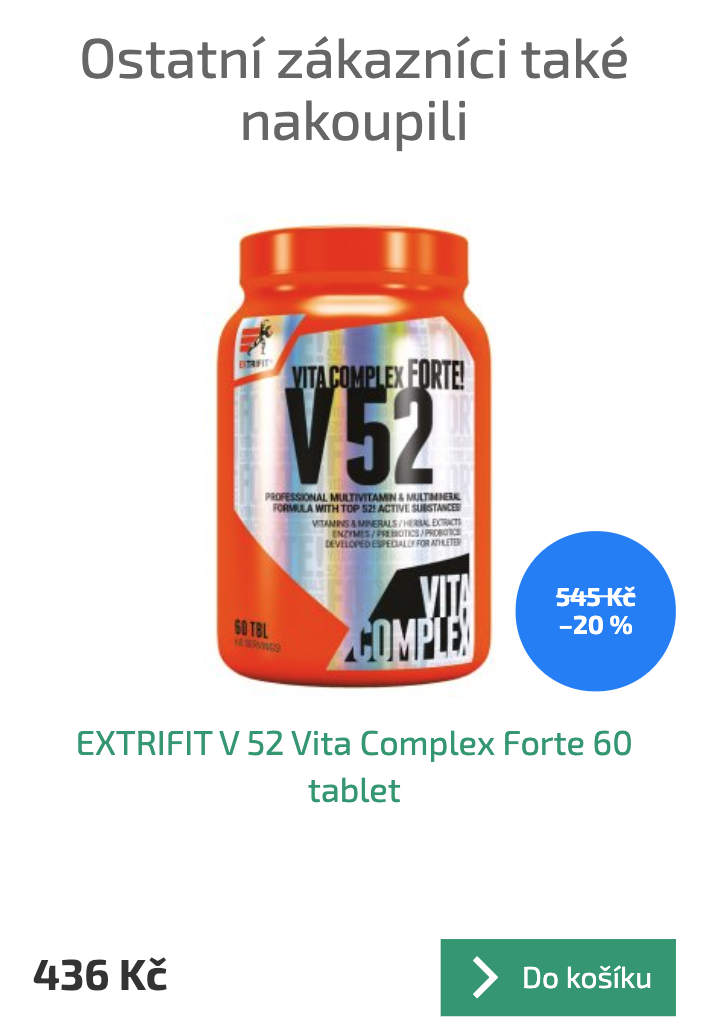
\includegraphics[width=0.5\linewidth]{media/beason.cz-cross-selling.png}
        \caption{An example of cross-selling as "Pressured Selling" dark pattern found on webshop beason.cz. This dark pattern appears in a pop-up window immediately after users add a product to a cart. "Ostatní zákazníci také nakoupili" can be translated into English as "Other customers also purchased".}
        \label{fig:cross-selling}
    \end{figure}

    \subsubsection*{Free Shipping}
    Many webshops allow free shipping after certain criteria are met. Such a criterion is the price of the purchase. This can affect a customer's judgment of spending more money on products he initially did not want, only to have free shipping (Some webshops even offer gifts for free). In addition, webshops make users very aware of the need to purchase more products to get free shipping. In total, 132 instances of this dark pattern are present in the dataset of dark patterns.

    As the cross-selling above, this is also a type of "Pressured Selling" dark pattern, and both are often used together. Figure \ref{fig:free-shipping} shows an instance of this dark dark pattern.

    \begin{figure}[ht]
        \centering
        
\includegraphics[width=1\linewidth]{media/beason.cz-free-shipping.png}
        \caption{An example of dark pattern "Pressured Selling" found on beason.cz. This dark pattern offers free shipping if a customer purchases for higher price. "Objednejte ještě za 900 Kč a budete mít dopravu ZDARMA" can be translated as "Order for another 900 CZK and you will get free shipping".}
        \label{fig:free-shipping}
    \end{figure}

    \subsubsection*{Heureka's Satisfaction Survey}
    High credibility is very important for webshops\cite{good-reviews}. For Czech webshops, good reviews on the Heureka portal can earn a certain amount of credibility. In addition, if a webshop is involved in the "Approved by Customers "program (which adds even more credibility), the review can be uploaded to the portal only by accessing it via a special link. This link is sent to the customer's e-mail if he/she gives his/her consent. However, this consent is often unconscious, as it manifests the "Trick Questions" dark pattern. In this case, it uses a double negation in the sentence, as can be seen in Figure \ref{fig:good-reviews}.
    
    \begin{figure}[ht]
        \centering
        
\includegraphics[width=0.7\linewidth]{media/levnelyze.cz-heureka.png}
        \caption{An example of "Trick Questions" dark pattern, which uses double negation in the sentence. The user may think that he is not giving his consent to the webshop for sending satisfaction surveys by not checking the checkbox. "Nesouhlasím  se zasláním ..." can be translated as "I do not agree with ..."}
        \label{fig:good-reviews}
    \end{figure}